\documentclass[twoside]{book}

% Packages required by doxygen
\usepackage{calc}
\usepackage{doxygen}
\usepackage{graphicx}
\usepackage[utf8]{inputenc}
\usepackage{makeidx}
\usepackage{multicol}
\usepackage{multirow}
\usepackage{textcomp}
\usepackage[table]{xcolor}

% Font selection
\usepackage[T1]{fontenc}
\usepackage{mathptmx}
\usepackage[scaled=.90]{helvet}
\usepackage{courier}
\usepackage{amssymb}
\usepackage{sectsty}
\renewcommand{\familydefault}{\sfdefault}
\allsectionsfont{%
  \fontseries{bc}\selectfont%
  \color{darkgray}%
}
\renewcommand{\DoxyLabelFont}{%
  \fontseries{bc}\selectfont%
  \color{darkgray}%
}

% Page & text layout
\usepackage{geometry}
\geometry{%
  a4paper,%
  top=2.5cm,%
  bottom=2.5cm,%
  left=2.5cm,%
  right=2.5cm%
}
\tolerance=750
\hfuzz=15pt
\hbadness=750
\setlength{\emergencystretch}{15pt}
\setlength{\parindent}{0cm}
\setlength{\parskip}{0.2cm}
\makeatletter
\renewcommand{\paragraph}{%
  \@startsection{paragraph}{4}{0ex}{-1.0ex}{1.0ex}{%
    \normalfont\normalsize\bfseries\SS@parafont%
  }%
}
\renewcommand{\subparagraph}{%
  \@startsection{subparagraph}{5}{0ex}{-1.0ex}{1.0ex}{%
    \normalfont\normalsize\bfseries\SS@subparafont%
  }%
}
\makeatother

% Headers & footers
\usepackage{fancyhdr}
\pagestyle{fancyplain}
\fancyhead[LE]{\fancyplain{}{\bfseries\thepage}}
\fancyhead[CE]{\fancyplain{}{}}
\fancyhead[RE]{\fancyplain{}{\bfseries\leftmark}}
\fancyhead[LO]{\fancyplain{}{\bfseries\rightmark}}
\fancyhead[CO]{\fancyplain{}{}}
\fancyhead[RO]{\fancyplain{}{\bfseries\thepage}}
\fancyfoot[LE]{\fancyplain{}{}}
\fancyfoot[CE]{\fancyplain{}{}}
\fancyfoot[RE]{\fancyplain{}{\bfseries\scriptsize Generated on Wed May 25 2016 17\-:07\-:56 for kukadu by Doxygen }}
\fancyfoot[LO]{\fancyplain{}{\bfseries\scriptsize Generated on Wed May 25 2016 17\-:07\-:56 for kukadu by Doxygen }}
\fancyfoot[CO]{\fancyplain{}{}}
\fancyfoot[RO]{\fancyplain{}{}}
\renewcommand{\footrulewidth}{0.4pt}
\renewcommand{\chaptermark}[1]{%
  \markboth{#1}{}%
}
\renewcommand{\sectionmark}[1]{%
  \markright{\thesection\ #1}%
}

% Indices & bibliography
\usepackage{natbib}
\usepackage[titles]{tocloft}
\setcounter{tocdepth}{3}
\setcounter{secnumdepth}{5}
\makeindex

% Hyperlinks (required, but should be loaded last)
\usepackage{ifpdf}
\ifpdf
  \usepackage[pdftex,pagebackref=true]{hyperref}
\else
  \usepackage[ps2pdf,pagebackref=true]{hyperref}
\fi
\hypersetup{%
  colorlinks=true,%
  linkcolor=blue,%
  citecolor=blue,%
  unicode%
}

% Custom commands
\newcommand{\clearemptydoublepage}{%
  \newpage{\pagestyle{empty}\cleardoublepage}%
}


%===== C O N T E N T S =====

\begin{document}

% Titlepage & ToC
\hypersetup{pageanchor=false}
\pagenumbering{roman}
\begin{titlepage}
\vspace*{7cm}
\begin{center}%
{\Large kukadu \\[1ex]\large 0.\-1a }\\
\vspace*{1cm}
{\large Generated by Doxygen 1.8.6}\\
\vspace*{0.5cm}
{\small Wed May 25 2016 17:07:56}\\
\end{center}
\end{titlepage}
\clearemptydoublepage
\tableofcontents
\clearemptydoublepage
\pagenumbering{arabic}
\hypersetup{pageanchor=true}

%--- Begin generated contents ---
\chapter{kukadu Tutorials}
\label{index}\hypertarget{index}{}\hypertarget{index_introduction}{}\section{Introduction}\label{index_introduction}
\hyperlink{introductionpage}{Introduction} \hypertarget{index_installation}{}\section{Installation}\label{index_installation}
\hyperlink{installationpage}{Installation} \hypertarget{index_gettingstarted}{}\section{Getting Started}\label{index_gettingstarted}
\hyperlink{gettingstartedpage}{Getting Started} \hypertarget{index_modules}{}\section{kukadu Modules}\label{index_modules}
\hyperlink{modulespage}{Modules} \hypertarget{index_robot}{}\subsection{The robot module}\label{index_robot}
\hyperlink{robotpage}{The robot module} \hypertarget{index_kinematics}{}\subsection{The kinematics and Planning module}\label{index_kinematics}
\hyperlink{kinematicspage}{The kinematics module} \hypertarget{index_control}{}\subsection{The control module}\label{index_control}
\hyperlink{controlpage}{The control module} \hypertarget{index_ml}{}\subsection{The machine learning module}\label{index_ml}
\hyperlink{mlpage}{The machine learning module} 
\chapter{Introduction}
\label{introductionpage}
\hypertarget{introductionpage}{}
kukadu is a software framework for robotics applications. It was used exensively in the lab of the \href{http://iis.uibk.ac.at}{\tt Intelligent and Interactive} systems group at the University of Innsbruck. It supports several different modules that are essential for robotics applications such as
\begin{DoxyItemize}
\item Robot control (\hyperlink{robotpage}{The robot module})
\item Kinematics and path planning (\hyperlink{kinematicspage}{The kinematics module})
\item Robust control policies (\hyperlink{controlpage}{The control module})
\item Machine learning (\hyperlink{mlpage}{The machine learning module})
\begin{DoxyItemize}
\item Regression
\item Classification
\item Kernel Methods
\item Reinforcement Learning
\end{DoxyItemize}
\end{DoxyItemize}

kukadu is written in C++ and supports usage in combination with \href{http://www.ros.org/}{\tt R\-O\-S}. It provides several general interfaces and implements it with state of the art methods from control, machine learning and robotic manipulation.

This document provides a setup guide (\hyperlink{installationpage}{Installation}) including a recommendation on how to develop kukadu software using \href{https://www.qt.io/ide/}{\tt Qt\-Creator}. Further, several tutorials and an A\-P\-I documentation is given.

Next (\hyperlink{installationpage}{Installation}) 
\chapter{Installation}
\label{installationpage}
\hypertarget{installationpage}{}
kukadu requires a current \href{http://www.ros.org/}{\tt R\-O\-S} system installed on your P\-C. We recommend R\-O\-S Indigo, however, using kukadu with any later version of R\-O\-S should not yield any problem. An installation guide for different operating systems can be found \href{http://wiki.ros.org/indigo/Installation}{\tt here}. Currently, kukadu is only supported with Ubuntu ($>$= 14.\-10) and a gcc compiler that supports at least C++11.

As kukadu provides a clean interface to a wide range of robotics applications and state-\/of-\/the art methods, several dependencies have to be installed.


\begin{DoxyCode}
sudo apt-\textcolor{keyword}{get} install libgsl0-dev gnuplot gnuplot-x11 libarmadillo-dev libboost-all-dev libncurses5-dev 
      libarmadillo-dev liballegro5-dev ros-indigo-pcl-ros ros-indigo-moveit-ros-planning-\textcolor{keyword}{interface }python3.4-dev 
      liblapacke-dev gtk+2.0 bison build-essential cmake doxygen fabric flex freeglut3-dev g++ gcc gfortran git-core 
      gnuplot graphviz-dev libann-dev libcv-dev libcvaux-dev libdc1394-22-dev libf2c2-dev libgtest-dev libgtkglext1-
      dev libhighgui-dev liblapack-dev libplib-dev libqhull-dev libsdl1.2-dev libx11-dev libx11-dev libxi-dev 
      libxmu-dev make meld python-nose python-unittest2 realpath regexxer swig2.0 tcl8.5-dev tk-dev tk8.5-dev 
      libfreenect-dev qt5-default ros-indigo-desktop-full ros-indigo-cob-common ros-indigo-ros-comm ros-indigo-geometry 
      ros-indigo-common-msgs ros-indigo-control-msgs ros-indigo-geometry-experimental libgsl0ldbl libgsl0-dev 
      libgstreamer0.10-dev libgstreamer-plugins-base0.10-dev ros-indigo-moveit-core ros-indigo-moveit-ros-planning ros-
      indigo-moveit-ros-planning-interface libghc-zlib-dev zlibc zlib1g-dbg zlib-bin ros-indigo-qt-build libqwt6 
      libqwt-dev libsdl1.2-dev ros-indigo-moveit-full ros-indigo-cmake-modules ros-indigo-map-msgs ros-indigo-
      controller-manager
\end{DoxyCode}


After installing the dependencies, you can clone kukadu to a \href{http://wiki.ros.org/catkin}{\tt catkin} workspace from our \href{https://git-scm.com/}{\tt Git} repository. If you are new to programming under R\-O\-S, you might be interested in the \href{http://wiki.ros.org/catkin/Tutorials}{\tt catkin tutorial}. You can find the kukadu Git repository \href{https://github.com/shangl/kukadu}{\tt here}. If you are not familiar with Git, simply go to your C\-A\-T\-K\-I\-N\-\_\-\-D\-I\-R/src directory and insert the following line to your terminal 
\begin{DoxyCode}
git clone --recursive https:\textcolor{comment}{//github.com/shangl/kukadu.git}
\end{DoxyCode}
 After cloning the repository, you can start compiling it by change to the root of your catkin workspace and typing 
\begin{DoxyCode}
catkin\_make
\end{DoxyCode}
 After the successful compilation kukadu is ready and you may continue with the next section (\hyperlink{gettingstartedpage}{Getting Started}). 
\chapter{Getting Started}
\label{gettingstartedpage}
\hypertarget{gettingstartedpage}{}
T\-O\-D\-O\-: here should be an example on how to start kukadu with a simulator example and a test script that is actually moving

Prev (\hyperlink{installationpage}{Installation}), Next (\hyperlink{modulespage}{Modules}) 
\chapter{Modules}
\label{modulespage}
\hypertarget{modulespage}{}
Currently, kukadu consists for 4 major modules\-:
\begin{DoxyItemize}
\item The robot module (\hyperlink{robotpage}{The robot module})\-: The robot module is the interface to a concrete robot. It provides an interface that defines what kukadu expects a robot to be able to do. If this interface is implemented for a specific robot, the complete stack of the framework is available.
\item The kinematics module (\hyperlink{kinematicspage}{The kinematics module})\-: As the name already says, the kinematics module provides kinematics for a given robot. It includes interfaces and implementations for forward and inverse kinematics as well as path planning functionality. The only prerequisite is an appropriate robot model in U\-R\-D\-F format. Currently, interfaces to Move\-It and K\-O\-M\-O are available.
\item The control module (\hyperlink{controlpage}{The control module})\-: The control module provides interfaces for control algorithms as well as certain implementations of these interfaces such as D\-M\-Ps and splines.
\item The machine learning module (\hyperlink{mlpage}{The machine learning module})\-: The machine learning module provides interfaces for supervised learning and reinforcement learning. Further, these interfaces are implemented for several methods such as
\begin{DoxyItemize}
\item Linear regression
\item Locally weighted regression
\item Gaussian process regression
\item S\-V\-M
\item Control policy reinforcement learning (Po\-W\-E\-R)
\item Reinforcement learning (Projective simulation, Monte carlo R\-L, Q-\/\-Learning, S\-A\-R\-S\-A)
\end{DoxyItemize}
\end{DoxyItemize}

Prev (\hyperlink{gettingstartedpage}{Getting Started}), Next (\hyperlink{robotpage}{The robot module}) 
\chapter{The robot module}
\label{robotpage}
\hypertarget{robotpage}{}
The \hyperlink{group__Robot}{Robot} module is the interface to a concrete robot. It provides an interface that defines what kukadu expects a robot to be able to do. If this interface is implemented for a specific robot, the complete stack of the framework is available.

The major interface is the abstract \hyperlink{classkukadu_1_1ControlQueue}{kukadu\-::\-Control\-Queue} class. It defines all the functions that are available for a robot (e.\-g. a robotic arm) without the robot base. If you want to bind kukadu to the robot in your lab, you have to implement the pure virtual functions of the \hyperlink{classkukadu_1_1ControlQueue}{kukadu\-::\-Control\-Queue}. Currently, there exist 2 implementations of \hyperlink{classkukadu_1_1ControlQueue}{kukadu\-::\-Control\-Queue}\-:
\begin{DoxyItemize}
\item \hyperlink{classkukadu_1_1KukieControlQueue}{kukadu\-::\-Kukie\-Control\-Queue}\-: Binds the kukadu framework to robots for which the \href{https://iis.uibk.ac.at/intranet/projects/robot/armtopics}{\tt kukie} framework is available. Kukie is a robot control framework based on R\-O\-S that defines certain topics and services for low-\/level robot control. Check out the kukie page to find out, if kukie is available for your system.
\item \hyperlink{classkukadu_1_1PlottingControlQueue}{kukadu\-::\-Plotting\-Control\-Queue}\-: Provides the kukadu functionility independent of the actual robot. With the \hyperlink{classkukadu_1_1PlottingControlQueue}{kukadu\-::\-Plotting\-Control\-Queue} no robot can be controlled, but it can be used as dummy robot in order to test other functionality. The \hyperlink{classkukadu_1_1PlottingControlQueue}{kukadu\-::\-Plotting\-Control\-Queue} simply ignores all submitted control commands.
\end{DoxyItemize}

\section*{\hyperlink{classkukadu_1_1KukieControlQueue}{kukadu\-::\-Kukie\-Control\-Queue}}

The following code snippet shows how to use the \hyperlink{classkukadu_1_1KukieControlQueue}{kukadu\-::\-Kukie\-Control\-Queue}. In order to make the program run, make sure that the kukie system is started (e.\-g. by starting the simulator or the real robot). 
\begin{DoxyCodeInclude}
1 \textcolor{preprocessor}{#include <kukadu/kukadu.hpp>}
2 
3 \textcolor{keyword}{using namespace }std;
4 \textcolor{keyword}{using namespace }kukadu;
5 
6 \textcolor{keywordtype}{int} main(\textcolor{keywordtype}{int} argc, \textcolor{keywordtype}{char}** args) \{
7 
8     cout << \textcolor{stringliteral}{"setting up ros node"} << endl;
9     ros::init(argc, args, \textcolor{stringliteral}{"kukadu\_controlqueue\_demo"}); ros::NodeHandle node; sleep(1);
10     ros::AsyncSpinner spinner(10); spinner.start();
11 
12     cout << \textcolor{stringliteral}{"setting up control queue"} << endl;
13     \textcolor{keyword}{auto} realLeftQueue = make\_shared<KukieControlQueue>(\textcolor{stringliteral}{"simulation"}, \textcolor{stringliteral}{"left\_arm"}, node);
14 
15     cout << \textcolor{stringliteral}{"starting queue"} << endl;
16     \textcolor{keyword}{auto} realLqThread = realLeftQueue->startQueue();
17 
18     cout << \textcolor{stringliteral}{"switching to impedance mode if it is not there yet"} << endl;
19     \textcolor{keywordflow}{if}(realLeftQueue->getCurrentMode() != KukieControlQueue::KUKA\_JNT\_IMP\_MODE) \{
20         realLeftQueue->stopCurrentMode();
21         realLeftQueue->switchMode(KukieControlQueue::KUKA\_JNT\_IMP\_MODE);
22     \}
23 
24     \textcolor{comment}{// joint point to point movement in order to go to the start position}
25     \textcolor{comment}{// remark: you only define where to go, not how to get there}
26     realLeftQueue->jointPtp(stdToArmadilloVec(\{-1.0, 1.0, -0.5, 0.0, 0.0, 0.0, 0.0\}));
27 
28     \textcolor{comment}{// retrieving the current joint state of the robot after the joint}
29     \textcolor{comment}{// point to point movement}
30     \textcolor{keyword}{auto} startState = realLeftQueue->getCurrentJoints().joints;
31 
32     \textcolor{comment}{// execution a trajectory for the 3rd joint (i.e. rotation the arm)}
33     \textcolor{comment}{// here you also provide HOW to get to the target}
34     \textcolor{keywordflow}{for}(\textcolor{keyword}{auto} currentState = startState; currentState(2) < startState(2) + 1.0; currentState(2) += 0.005) \{
35         \textcolor{comment}{// sending a the next desired position}
36         realLeftQueue->move(currentState);
37         \textcolor{comment}{// the queue has an intrinsic clock, so you can wait until the packet has been}
38         \textcolor{comment}{// submit in order to not send the positions too fast}
39         realLeftQueue->synchronizeToQueue(1);
40     \}
41 
42     cout << \textcolor{stringliteral}{"execution done"} << endl;
43 
44     \textcolor{comment}{/****** done with moving? --> clean up everything and quit *******/}
45 
46     \textcolor{comment}{// leaves the mode for robot movement}
47     realLeftQueue->stopCurrentMode();
48 
49     \textcolor{comment}{// stops the queue}
50     realLeftQueue->stopQueue();
51 
52     \textcolor{comment}{// waits until everything has stopped}
53     realLqThread->join();
54 
55 \}
\end{DoxyCodeInclude}


\subsection*{Code description}

Lets have a closer look to the tutorial code. First of all, the kukadu library needs to be included (line 1). All kukadu functionality is contained in the kukadu namespace (line 4). kukadu is a framework embedded in R\-O\-S, so the first action that should be done is setting up the ros connection (lines 8 -\/ 10).

The direct connection to the robot is given by the \hyperlink{classkukadu_1_1ControlQueue}{kukadu\-::\-Control\-Queue} interface. This means that an implementation of that interface should be instantiated per robot. This is done line 13 where an instance of the \hyperlink{classkukadu_1_1KukieControlQueue}{kukadu\-::\-Kukie\-Control\-Queue} is created for the left arm in simulation. In line 16, the queue is started -\/ so the queue is ready to go. However, you can't move the robot until it is switched to an appropriate control mode (lines 19 -\/ 22). Afterwards, the robot is ready to go, so you should pay special attention to it.

In the first step, we can make the robot arm move by a simple point to point movement (line 26). This means that you don't need to take care how the robot reaches the desired position. All the path planning is done automatically by the system and you only need to execute the \hyperlink{classkukadu_1_1ControlQueue_ad11059100321b24a1af8ef7de8314353}{kukadu\-::\-Control\-Queue\-::joint\-Ptp()} function (there is also a method for \hyperlink{classkukadu_1_1ControlQueue_a1bfa23a8ce6319f6ef0ed9208e896054}{kukadu\-::\-Control\-Queue\-::cartesian\-Ptp()}). This function blocks until the last packet is sent to the robot -\/ however, it is not guaranteed that the robot reaches that position with precision. You can check if it was precise enough by looking at the returned joint positions.

After the Pt\-P execution the program retrieves the current joint state of the robot with the kukadu\-::\-Controlqueue\-::get\-Current\-Joints() function. There is also a function for the Cartesian state named \hyperlink{classkukadu_1_1ControlQueue_a9e79e1d0d9697bbf146d66a2d01fea9e}{kukadu\-::\-Control\-Queue\-::get\-Current\-Cartesian\-Pose()}.

The final step of the demo program is the execution of a specific trajectory. In this case you can not only define the target but also the path the robot should use to get there. In general, the \hyperlink{classkukadu_1_1ControlQueue}{kukadu\-::\-Control\-Queue} is a clocked queue that submits one joint packet per clock cycle. This packet is then submitted to the robot. If no new packet is set, then the robot is commanded to stay at the current position. In lines 34 -\/ 40, a specific trajectory is submitted to the queue by added one packet per clock cycle using the \hyperlink{classkukadu_1_1ControlQueue_aca70a978b2950d7c9ab99d55c5977eec}{kukadu\-::\-Control\-Queue\-::move()} function. This procedure is synchronized to the queue by the \hyperlink{classkukadu_1_1ControlQueue_a324484e79a5505656a32d9f32054e5d0}{kukadu\-::\-Control\-Queue\-::synchronize\-To\-Queue()} function. This function blocks until at most N packets (in this case N = 1) is left in the queue. This makes sure that your program stays in synch with the queue. However, if you dont use this function, all packets are added to the queue at once and the queue sent on packet per clock cycle. However, you need to make sure to synchronize with the queue otherwise then.

In lines 44 -\/ 53, the queue is disconnected from the robot. The most important part is to leave the execution mode (line 47). After leaving the execution mode, the queue is stopped (line 50) and the program waits until the queue is stopped completely (line 53).

Prev (\hyperlink{modulespage}{Modules}), Next (\hyperlink{kinematicspage}{The kinematics module}) 
\chapter{The kinematics module}
\label{kinematicspage}
\hypertarget{kinematicspage}{}
Prev (\hyperlink{robotpage}{The robot module}), Next (\hyperlink{controlpage}{The control module}) 
\chapter{The control module}
\label{controlpage}
\hypertarget{controlpage}{}
Prev (\hyperlink{kinematicspage}{The kinematics module}), Next (\hyperlink{mlpage}{The machine learning module}) 
\chapter{The machine learning module}
\label{mlpage}
\hypertarget{mlpage}{}
Prev (\hyperlink{controlpage}{The control module}) 
\chapter{Module Index}
\section{Modules}
Here is a list of all modules\-:\begin{DoxyCompactList}
\item \contentsline{section}{Control\-Policy\-Framework}{\pageref{group__ControlPolicyFramework}}{}
\item \contentsline{section}{Learning\-Framework}{\pageref{group__LearningFramework}}{}
\item \contentsline{section}{Control}{\pageref{group__Control}}{}
\item \contentsline{section}{Fri\-Remote\-Lib}{\pageref{group__friRemoteLib}}{}
\end{DoxyCompactList}

\chapter{Namespace Index}
\section{Namespace List}
Here is a list of all documented namespaces with brief descriptions\-:\begin{DoxyCompactList}
\item\contentsline{section}{\hyperlink{namespacekukadu}{kukadu} \\*A C++ interface to gnuplot }{\pageref{namespacekukadu}}{}
\end{DoxyCompactList}

\chapter{Hierarchical Index}
\section{Class Hierarchy}
This inheritance list is sorted roughly, but not completely, alphabetically\-:\begin{DoxyCompactList}
\item \contentsline{section}{kukadu\-:\-:armacomp}{\pageref{structkukadu_1_1armacomp}}{}
\item \contentsline{section}{kukadu\-:\-:clip\-\_\-compare}{\pageref{structkukadu_1_1clip__compare}}{}
\item \contentsline{section}{kukadu\-:\-:Clusters}{\pageref{classkukadu_1_1Clusters}}{}
\item \contentsline{section}{kukadu\-:\-:Constraint}{\pageref{classkukadu_1_1Constraint}}{}
\begin{DoxyCompactList}
\item \contentsline{section}{kukadu\-:\-:Move\-It\-Constraint}{\pageref{classkukadu_1_1MoveItConstraint}}{}
\item \contentsline{section}{kukadu\-:\-:Table\-Constraint}{\pageref{classkukadu_1_1TableConstraint}}{}
\end{DoxyCompactList}
\item \contentsline{section}{kukadu\-:\-:Controller}{\pageref{classkukadu_1_1Controller}}{}
\begin{DoxyCompactList}
\item \contentsline{section}{kukadu\-:\-:Complex\-Controller}{\pageref{classkukadu_1_1ComplexController}}{}
\item \contentsline{section}{kukadu\-:\-:Sensing\-Controller}{\pageref{classkukadu_1_1SensingController}}{}
\item \contentsline{section}{kukadu\-:\-:Trajectory\-Executor}{\pageref{classkukadu_1_1TrajectoryExecutor}}{}
\begin{DoxyCompactList}
\item \contentsline{section}{kukadu\-:\-:D\-M\-P\-Executor}{\pageref{classkukadu_1_1DMPExecutor}}{}
\end{DoxyCompactList}
\end{DoxyCompactList}
\item \contentsline{section}{kukadu\-:\-:Controller\-Result}{\pageref{classkukadu_1_1ControllerResult}}{}
\begin{DoxyCompactList}
\item \contentsline{section}{kukadu\-:\-:Haptic\-Controller\-Result}{\pageref{classkukadu_1_1HapticControllerResult}}{}
\end{DoxyCompactList}
\item \contentsline{section}{kukadu\-:\-:Cost\-Computer}{\pageref{classkukadu_1_1CostComputer}}{}
\begin{DoxyCompactList}
\item \contentsline{section}{kukadu\-:\-:Terminal\-Cost\-Computer}{\pageref{classkukadu_1_1TerminalCostComputer}}{}
\item \contentsline{section}{kukadu\-:\-:Trajectory\-Based\-Reward}{\pageref{classkukadu_1_1TrajectoryBasedReward}}{}
\begin{DoxyCompactList}
\item \contentsline{section}{kukadu\-:\-:Dmp\-Reward\-Computer}{\pageref{classkukadu_1_1DmpRewardComputer}}{}
\item \contentsline{section}{kukadu\-:\-:Sample\-Reward\-Computer}{\pageref{classkukadu_1_1SampleRewardComputer}}{}
\end{DoxyCompactList}
\end{DoxyCompactList}
\item \contentsline{section}{kukadu\-:\-:Destroyable\-Object}{\pageref{classkukadu_1_1DestroyableObject}}{}
\begin{DoxyCompactList}
\item \contentsline{section}{kukadu\-:\-:Control\-Queue}{\pageref{classkukadu_1_1ControlQueue}}{}
\begin{DoxyCompactList}
\item \contentsline{section}{kukadu\-:\-:Kukie\-Control\-Queue}{\pageref{classkukadu_1_1KukieControlQueue}}{}
\item \contentsline{section}{kukadu\-:\-:Plotting\-Control\-Queue}{\pageref{classkukadu_1_1PlottingControlQueue}}{}
\end{DoxyCompactList}
\item \contentsline{section}{kukadu\-:\-:Generic\-Hand}{\pageref{classkukadu_1_1GenericHand}}{}
\begin{DoxyCompactList}
\item \contentsline{section}{kukadu\-:\-:Ros\-Schunk}{\pageref{classkukadu_1_1RosSchunk}}{}
\begin{DoxyCompactList}
\item \contentsline{section}{kukadu\-:\-:Plotting\-Hand}{\pageref{classkukadu_1_1PlottingHand}}{}
\end{DoxyCompactList}
\end{DoxyCompactList}
\end{DoxyCompactList}
\item \contentsline{section}{kukadu\-:\-:D\-M\-P\-Base}{\pageref{classkukadu_1_1DMPBase}}{}
\item \contentsline{section}{kukadu\-:\-:D\-M\-P\-Reinforcer}{\pageref{classkukadu_1_1DMPReinforcer}}{}
\item exception\begin{DoxyCompactList}
\item \contentsline{section}{Kukadu\-Exception}{\pageref{classKukaduException}}{}
\end{DoxyCompactList}
\item \contentsline{section}{kukadu\-:\-:Fit\-Cube}{\pageref{structkukadu_1_1FitCube}}{}
\item \contentsline{section}{kukadu\-:\-:General\-Dmp\-Learner}{\pageref{classkukadu_1_1GeneralDmpLearner}}{}
\begin{DoxyCompactList}
\item \contentsline{section}{kukadu\-:\-:Cartesian\-D\-M\-P\-Learner}{\pageref{classkukadu_1_1CartesianDMPLearner}}{}
\item \contentsline{section}{kukadu\-:\-:Joint\-D\-M\-P\-Learner}{\pageref{classkukadu_1_1JointDMPLearner}}{}
\end{DoxyCompactList}
\item \contentsline{section}{kukadu\-:\-:General\-Fitter}{\pageref{classkukadu_1_1GeneralFitter}}{}
\item \contentsline{section}{kukadu\-:\-:General\-Reinforcer}{\pageref{classkukadu_1_1GeneralReinforcer}}{}
\begin{DoxyCompactList}
\item \contentsline{section}{kukadu\-:\-:Gradient\-Descent}{\pageref{classkukadu_1_1GradientDescent}}{}
\item \contentsline{section}{kukadu\-:\-:Po\-W\-E\-R}{\pageref{classkukadu_1_1PoWER}}{}
\end{DoxyCompactList}
\item \contentsline{section}{kukadu\-:\-:Generic\-Generalizer}{\pageref{classkukadu_1_1GenericGeneralizer}}{}
\begin{DoxyCompactList}
\item \contentsline{section}{kukadu\-:\-:D\-M\-P\-Generalizer}{\pageref{classkukadu_1_1DMPGeneralizer}}{}
\end{DoxyCompactList}
\item \contentsline{section}{kukadu\-:\-:Generic\-Kernel}{\pageref{classkukadu_1_1GenericKernel}}{}
\begin{DoxyCompactList}
\item \contentsline{section}{kukadu\-:\-:Gaussian\-Kernel}{\pageref{classkukadu_1_1GaussianKernel}}{}
\item \contentsline{section}{kukadu\-:\-:Quadratic\-Kernel}{\pageref{classkukadu_1_1QuadraticKernel}}{}
\item \contentsline{section}{kukadu\-:\-:Tricube\-Kernel}{\pageref{classkukadu_1_1TricubeKernel}}{}
\end{DoxyCompactList}
\item \contentsline{section}{kukadu\-:\-:Gnuplot}{\pageref{classkukadu_1_1Gnuplot}}{}
\item \contentsline{section}{kukadu\-:\-:gsl\-\_\-delete\-\_\-expression}{\pageref{structkukadu_1_1gsl__delete__expression}}{}
\item \contentsline{section}{kukadu\-:\-:Inf\-Theo\-Constraints}{\pageref{classkukadu_1_1InfTheoConstraints}}{}
\item \contentsline{section}{kukadu\-:\-:Kernel\-Regressor}{\pageref{classkukadu_1_1KernelRegressor}}{}
\begin{DoxyCompactList}
\item \contentsline{section}{kukadu\-:\-:Gaussian\-Process\-Regressor}{\pageref{classkukadu_1_1GaussianProcessRegressor}}{}
\item \contentsline{section}{kukadu\-:\-:L\-W\-R\-Regressor}{\pageref{classkukadu_1_1LWRRegressor}}{}
\end{DoxyCompactList}
\item \contentsline{section}{kukadu\-:\-:Kinect}{\pageref{classkukadu_1_1Kinect}}{}
\item \contentsline{section}{kukadu\-:\-:Kinematics}{\pageref{classkukadu_1_1Kinematics}}{}
\begin{DoxyCompactList}
\item \contentsline{section}{kukadu\-:\-:Komo\-Planner}{\pageref{classkukadu_1_1KomoPlanner}}{}
\item \contentsline{section}{kukadu\-:\-:Move\-It\-Kinematics}{\pageref{classkukadu_1_1MoveItKinematics}}{}
\end{DoxyCompactList}
\item K\-U\-K\-A\-D\-U\-\_\-\-E\-N\-A\-B\-L\-E\-\_\-\-S\-H\-A\-R\-E\-D\-\_\-\-F\-R\-O\-M\-\_\-\-T\-H\-I\-S\begin{DoxyCompactList}
\item \contentsline{section}{kukadu\-:\-:Clip}{\pageref{classkukadu_1_1Clip}}{}
\begin{DoxyCompactList}
\item \contentsline{section}{kukadu\-:\-:Action\-Clip}{\pageref{classkukadu_1_1ActionClip}}{}
\begin{DoxyCompactList}
\item \contentsline{section}{kukadu\-:\-:Controller\-Action\-Clip}{\pageref{classkukadu_1_1ControllerActionClip}}{}
\end{DoxyCompactList}
\item \contentsline{section}{kukadu\-:\-:Intermediate\-Event\-Clip}{\pageref{classkukadu_1_1IntermediateEventClip}}{}
\item \contentsline{section}{kukadu\-:\-:Percept\-Clip}{\pageref{classkukadu_1_1PerceptClip}}{}
\end{DoxyCompactList}
\item \contentsline{section}{kukadu\-:\-:Complex\-Controller}{\pageref{classkukadu_1_1ComplexController}}{}
\item \contentsline{section}{kukadu\-:\-:Control\-Queue}{\pageref{classkukadu_1_1ControlQueue}}{}
\item \contentsline{section}{kukadu\-:\-:Haptic\-Planner}{\pageref{classkukadu_1_1HapticPlanner}}{}
\end{DoxyCompactList}
\item \contentsline{section}{kukadu\-:\-:Kukadu\-Tokenizer}{\pageref{classkukadu_1_1KukaduTokenizer}}{}
\item \contentsline{section}{kukadu\-:\-:Mahalanobis}{\pageref{classkukadu_1_1Mahalanobis}}{}
\item \contentsline{section}{kukadu\-:\-:Mahalanobis\-Learner}{\pageref{classkukadu_1_1MahalanobisLearner}}{}
\begin{DoxyCompactList}
\item \contentsline{section}{kukadu\-:\-:Inf\-Theo\-Metric\-Learner}{\pageref{classkukadu_1_1InfTheoMetricLearner}}{}
\item \contentsline{section}{kukadu\-:\-:Togerson\-Metric\-Learner}{\pageref{classkukadu_1_1TogersonMetricLearner}}{}
\end{DoxyCompactList}
\item \contentsline{section}{mes\-\_\-result}{\pageref{structmes__result}}{}
\item \contentsline{section}{kukadu\-:\-:Path\-Planner}{\pageref{classkukadu_1_1PathPlanner}}{}
\begin{DoxyCompactList}
\item \contentsline{section}{kukadu\-:\-:Komo\-Planner}{\pageref{classkukadu_1_1KomoPlanner}}{}
\item \contentsline{section}{kukadu\-:\-:Move\-It\-Kinematics}{\pageref{classkukadu_1_1MoveItKinematics}}{}
\item \contentsline{section}{kukadu\-:\-:Simple\-Planner}{\pageref{classkukadu_1_1SimplePlanner}}{}
\end{DoxyCompactList}
\item \contentsline{section}{kukadu\-:\-:P\-C\-L\-Tools}{\pageref{classkukadu_1_1PCLTools}}{}
\item \contentsline{section}{P\-C\-Transformator}{\pageref{classPCTransformator}}{}
\begin{DoxyCompactList}
\item \contentsline{section}{kukadu\-:\-:Open\-Box\-Filter}{\pageref{classkukadu_1_1OpenBoxFilter}}{}
\item \contentsline{section}{kukadu\-:\-:Planar\-Cut\-Transformator}{\pageref{classkukadu_1_1PlanarCutTransformator}}{}
\end{DoxyCompactList}
\item \contentsline{section}{kukadu\-:\-:Planning\-Result}{\pageref{structkukadu_1_1PlanningResult}}{}
\item \contentsline{section}{kukadu\-:\-:Points\-Space}{\pageref{classkukadu_1_1PointsSpace}}{}
\item \contentsline{section}{kukadu\-:\-:Projective\-Simulator}{\pageref{classkukadu_1_1ProjectiveSimulator}}{}
\item \contentsline{section}{kukadu\-:\-:P\-S\-Evaluator}{\pageref{classkukadu_1_1PSEvaluator}}{}
\item \contentsline{section}{kukadu\-:\-:Query\-Point}{\pageref{classkukadu_1_1QueryPoint}}{}
\item \contentsline{section}{kukadu\-:\-:Reward}{\pageref{classkukadu_1_1Reward}}{}
\begin{DoxyCompactList}
\item \contentsline{section}{kukadu\-:\-:Complex\-Controller}{\pageref{classkukadu_1_1ComplexController}}{}
\item \contentsline{section}{kukadu\-:\-:Environment\-Reward}{\pageref{classkukadu_1_1EnvironmentReward}}{}
\item \contentsline{section}{kukadu\-:\-:Haptic\-Planner}{\pageref{classkukadu_1_1HapticPlanner}}{}
\item \contentsline{section}{kukadu\-:\-:Invasion\-Game\-Reward}{\pageref{classkukadu_1_1InvasionGameReward}}{}
\item \contentsline{section}{kukadu\-:\-:Manual\-Reward}{\pageref{classkukadu_1_1ManualReward}}{}
\item \contentsline{section}{kukadu\-:\-:Neverending\-Color\-Reward}{\pageref{classkukadu_1_1NeverendingColorReward}}{}
\item \contentsline{section}{kukadu\-:\-:Traffic\-Light\-Reward}{\pageref{classkukadu_1_1TrafficLightReward}}{}
\end{DoxyCompactList}
\item runtime\-\_\-error\begin{DoxyCompactList}
\item \contentsline{section}{kukadu\-:\-:Gnuplot\-Exception}{\pageref{classkukadu_1_1GnuplotException}}{}
\end{DoxyCompactList}
\item \contentsline{section}{kukadu\-:\-:Sensor\-Data}{\pageref{classkukadu_1_1SensorData}}{}
\item \contentsline{section}{kukadu\-:\-:Sensor\-Storage}{\pageref{classkukadu_1_1SensorStorage}}{}
\item \contentsline{section}{kukadu\-:\-:Tic\-Toc}{\pageref{classkukadu_1_1TicToc}}{}
\item \contentsline{section}{kukadu\-:\-:Trajectory}{\pageref{classkukadu_1_1Trajectory}}{}
\begin{DoxyCompactList}
\item \contentsline{section}{kukadu\-:\-:Dictionary\-Trajectory}{\pageref{classkukadu_1_1DictionaryTrajectory}}{}
\item \contentsline{section}{kukadu\-:\-:Single\-Sample\-Trajectory}{\pageref{classkukadu_1_1SingleSampleTrajectory}}{}
\begin{DoxyCompactList}
\item \contentsline{section}{kukadu\-:\-:Dmp}{\pageref{classkukadu_1_1Dmp}}{}
\begin{DoxyCompactList}
\item \contentsline{section}{kukadu\-:\-:Cartesian\-D\-M\-P}{\pageref{classkukadu_1_1CartesianDMP}}{}
\item \contentsline{section}{kukadu\-:\-:Joint\-Dmp}{\pageref{classkukadu_1_1JointDmp}}{}
\end{DoxyCompactList}
\end{DoxyCompactList}
\end{DoxyCompactList}
\item \contentsline{section}{trajectory\-\_\-learner\-\_\-internal}{\pageref{structtrajectory__learner__internal}}{}
\item \contentsline{section}{kukadu\-:\-:Trajectory\-Comparator}{\pageref{classkukadu_1_1TrajectoryComparator}}{}
\item \contentsline{section}{kukadu\-:\-:Trajectory\-Generator}{\pageref{classkukadu_1_1TrajectoryGenerator}}{}
\begin{DoxyCompactList}
\item \contentsline{section}{kukadu\-:\-:D\-M\-P\-Trajectory\-Generator}{\pageref{classkukadu_1_1DMPTrajectoryGenerator}}{}
\item \contentsline{section}{kukadu\-:\-:Poly\-Trajectory\-Generator}{\pageref{classkukadu_1_1PolyTrajectoryGenerator}}{}
\end{DoxyCompactList}
\item \contentsline{section}{kukadu\-:\-:Tree\-Drawer}{\pageref{classkukadu_1_1TreeDrawer}}{}
\item vector\begin{DoxyCompactList}
\item \contentsline{section}{kukadu\-:\-:Custom\-Set}{\pageref{classkukadu_1_1CustomSet}}{}
\end{DoxyCompactList}
\item \contentsline{section}{kukadu\-:\-:Vision\-Interface}{\pageref{classkukadu_1_1VisionInterface}}{}
\end{DoxyCompactList}

\chapter{Class Index}
\section{Class List}
Here are the classes, structs, unions and interfaces with brief descriptions\-:\begin{DoxyCompactList}
\item\contentsline{section}{\hyperlink{classkukadu_1_1ActionClip}{kukadu\-::\-Action\-Clip} }{\pageref{classkukadu_1_1ActionClip}}{}
\item\contentsline{section}{\hyperlink{structkukadu_1_1armacomp}{kukadu\-::armacomp} }{\pageref{structkukadu_1_1armacomp}}{}
\item\contentsline{section}{\hyperlink{classkukadu_1_1CartesianDMP}{kukadu\-::\-Cartesian\-D\-M\-P} }{\pageref{classkukadu_1_1CartesianDMP}}{}
\item\contentsline{section}{\hyperlink{classkukadu_1_1CartesianDMPLearner}{kukadu\-::\-Cartesian\-D\-M\-P\-Learner} \\*The Trajectory\-D\-M\-P\-Learner encapsulates the dmp learning process }{\pageref{classkukadu_1_1CartesianDMPLearner}}{}
\item\contentsline{section}{\hyperlink{classkukadu_1_1Clip}{kukadu\-::\-Clip} }{\pageref{classkukadu_1_1Clip}}{}
\item\contentsline{section}{\hyperlink{structkukadu_1_1clip__compare}{kukadu\-::clip\-\_\-compare} }{\pageref{structkukadu_1_1clip__compare}}{}
\item\contentsline{section}{\hyperlink{classkukadu_1_1Clusters}{kukadu\-::\-Clusters} }{\pageref{classkukadu_1_1Clusters}}{}
\item\contentsline{section}{\hyperlink{classkukadu_1_1ComplexController}{kukadu\-::\-Complex\-Controller} }{\pageref{classkukadu_1_1ComplexController}}{}
\item\contentsline{section}{\hyperlink{classkukadu_1_1Constraint}{kukadu\-::\-Constraint} }{\pageref{classkukadu_1_1Constraint}}{}
\item\contentsline{section}{\hyperlink{classkukadu_1_1Controller}{kukadu\-::\-Controller} }{\pageref{classkukadu_1_1Controller}}{}
\item\contentsline{section}{\hyperlink{classkukadu_1_1ControllerActionClip}{kukadu\-::\-Controller\-Action\-Clip} }{\pageref{classkukadu_1_1ControllerActionClip}}{}
\item\contentsline{section}{\hyperlink{classkukadu_1_1ControllerResult}{kukadu\-::\-Controller\-Result} }{\pageref{classkukadu_1_1ControllerResult}}{}
\item\contentsline{section}{\hyperlink{classkukadu_1_1ControlQueue}{kukadu\-::\-Control\-Queue} \\*Interface between the kukadu software stack and the robot hardware. If kukadu shall support another robot, the abstract methods need to be implemented according to the documentation. Then the kukadu software stack is available for usage with the robot }{\pageref{classkukadu_1_1ControlQueue}}{}
\item\contentsline{section}{\hyperlink{classkukadu_1_1CostComputer}{kukadu\-::\-Cost\-Computer} \\*Interface for reinforcement learning cost function computation used by \hyperlink{classkukadu_1_1DMPReinforcer}{D\-M\-P\-Reinforcer} }{\pageref{classkukadu_1_1CostComputer}}{}
\item\contentsline{section}{\hyperlink{classkukadu_1_1CustomSet}{kukadu\-::\-Custom\-Set} }{\pageref{classkukadu_1_1CustomSet}}{}
\item\contentsline{section}{\hyperlink{classkukadu_1_1DestroyableObject}{kukadu\-::\-Destroyable\-Object} \\*Interface defining a callback function }{\pageref{classkukadu_1_1DestroyableObject}}{}
\item\contentsline{section}{\hyperlink{classkukadu_1_1DictionaryTrajectory}{kukadu\-::\-Dictionary\-Trajectory} }{\pageref{classkukadu_1_1DictionaryTrajectory}}{}
\item\contentsline{section}{\hyperlink{classkukadu_1_1Dmp}{kukadu\-::\-Dmp} }{\pageref{classkukadu_1_1Dmp}}{}
\item\contentsline{section}{\hyperlink{classkukadu_1_1DMPBase}{kukadu\-::\-D\-M\-P\-Base} }{\pageref{classkukadu_1_1DMPBase}}{}
\item\contentsline{section}{\hyperlink{classkukadu_1_1DMPExecutor}{kukadu\-::\-D\-M\-P\-Executor} \\*This class is responsible for dmp execution }{\pageref{classkukadu_1_1DMPExecutor}}{}
\item\contentsline{section}{\hyperlink{classkukadu_1_1DMPGeneralizer}{kukadu\-::\-D\-M\-P\-Generalizer} \\*This class is able to generalize task specific trajectories from previous examples }{\pageref{classkukadu_1_1DMPGeneralizer}}{}
\item\contentsline{section}{\hyperlink{classkukadu_1_1DMPReinforcer}{kukadu\-::\-D\-M\-P\-Reinforcer} \\*The \hyperlink{classkukadu_1_1DMPReinforcer}{D\-M\-P\-Reinforcer} provides a general framework for reinforcement learning }{\pageref{classkukadu_1_1DMPReinforcer}}{}
\item\contentsline{section}{\hyperlink{classkukadu_1_1DmpRewardComputer}{kukadu\-::\-Dmp\-Reward\-Computer} }{\pageref{classkukadu_1_1DmpRewardComputer}}{}
\item\contentsline{section}{\hyperlink{classkukadu_1_1DMPTrajectoryGenerator}{kukadu\-::\-D\-M\-P\-Trajectory\-Generator} \\*Implements the \hyperlink{classkukadu_1_1TrajectoryGenerator}{Trajectory\-Generator} interface for dynamic movement primitives }{\pageref{classkukadu_1_1DMPTrajectoryGenerator}}{}
\item\contentsline{section}{\hyperlink{classkukadu_1_1EnvironmentReward}{kukadu\-::\-Environment\-Reward} }{\pageref{classkukadu_1_1EnvironmentReward}}{}
\item\contentsline{section}{\hyperlink{structkukadu_1_1FitCube}{kukadu\-::\-Fit\-Cube} }{\pageref{structkukadu_1_1FitCube}}{}
\item\contentsline{section}{\hyperlink{classkukadu_1_1GaussianKernel}{kukadu\-::\-Gaussian\-Kernel} \\*Implements a Gaussian kernel according to the \hyperlink{classkukadu_1_1GenericKernel}{Generic\-Kernel} specifiction }{\pageref{classkukadu_1_1GaussianKernel}}{}
\item\contentsline{section}{\hyperlink{classkukadu_1_1GaussianProcessRegressor}{kukadu\-::\-Gaussian\-Process\-Regressor} \\*Implements the Gaussian process regression method }{\pageref{classkukadu_1_1GaussianProcessRegressor}}{}
\item\contentsline{section}{\hyperlink{classkukadu_1_1GeneralDmpLearner}{kukadu\-::\-General\-Dmp\-Learner} }{\pageref{classkukadu_1_1GeneralDmpLearner}}{}
\item\contentsline{section}{\hyperlink{classkukadu_1_1GeneralFitter}{kukadu\-::\-General\-Fitter} \\*Provides the generic part of the linear regression methods }{\pageref{classkukadu_1_1GeneralFitter}}{}
\item\contentsline{section}{\hyperlink{classkukadu_1_1GeneralReinforcer}{kukadu\-::\-General\-Reinforcer} \\*The \hyperlink{classkukadu_1_1GeneralReinforcer}{General\-Reinforcer} provides a general framework for reinforcement learning }{\pageref{classkukadu_1_1GeneralReinforcer}}{}
\item\contentsline{section}{\hyperlink{classkukadu_1_1GenericGeneralizer}{kukadu\-::\-Generic\-Generalizer} }{\pageref{classkukadu_1_1GenericGeneralizer}}{}
\item\contentsline{section}{\hyperlink{classkukadu_1_1GenericHand}{kukadu\-::\-Generic\-Hand} \\*The \hyperlink{classkukadu_1_1GenericHand}{Generic\-Hand} provides a very elementary interface to control robot hands mounted on a robot arm This class provides very an interface for the very basic functionalities such as \char`\"{}connect to hand\char`\"{} or \char`\"{}close hand\char`\"{} }{\pageref{classkukadu_1_1GenericHand}}{}
\item\contentsline{section}{\hyperlink{classkukadu_1_1GenericKernel}{kukadu\-::\-Generic\-Kernel} \\*Provides an interface for generic kernel functions }{\pageref{classkukadu_1_1GenericKernel}}{}
\item\contentsline{section}{\hyperlink{classkukadu_1_1Gnuplot}{kukadu\-::\-Gnuplot} }{\pageref{classkukadu_1_1Gnuplot}}{}
\item\contentsline{section}{\hyperlink{classkukadu_1_1GnuplotException}{kukadu\-::\-Gnuplot\-Exception} }{\pageref{classkukadu_1_1GnuplotException}}{}
\item\contentsline{section}{\hyperlink{classkukadu_1_1GradientDescent}{kukadu\-::\-Gradient\-Descent} }{\pageref{classkukadu_1_1GradientDescent}}{}
\item\contentsline{section}{\hyperlink{structkukadu_1_1gsl__delete__expression}{kukadu\-::gsl\-\_\-delete\-\_\-expression} }{\pageref{structkukadu_1_1gsl__delete__expression}}{}
\item\contentsline{section}{\hyperlink{classkukadu_1_1HapticControllerResult}{kukadu\-::\-Haptic\-Controller\-Result} }{\pageref{classkukadu_1_1HapticControllerResult}}{}
\item\contentsline{section}{\hyperlink{classkukadu_1_1HapticPlanner}{kukadu\-::\-Haptic\-Planner} }{\pageref{classkukadu_1_1HapticPlanner}}{}
\item\contentsline{section}{\hyperlink{classkukadu_1_1InfTheoConstraints}{kukadu\-::\-Inf\-Theo\-Constraints} }{\pageref{classkukadu_1_1InfTheoConstraints}}{}
\item\contentsline{section}{\hyperlink{classkukadu_1_1InfTheoMetricLearner}{kukadu\-::\-Inf\-Theo\-Metric\-Learner} }{\pageref{classkukadu_1_1InfTheoMetricLearner}}{}
\item\contentsline{section}{\hyperlink{classkukadu_1_1IntermediateEventClip}{kukadu\-::\-Intermediate\-Event\-Clip} }{\pageref{classkukadu_1_1IntermediateEventClip}}{}
\item\contentsline{section}{\hyperlink{classkukadu_1_1InvasionGameReward}{kukadu\-::\-Invasion\-Game\-Reward} }{\pageref{classkukadu_1_1InvasionGameReward}}{}
\item\contentsline{section}{\hyperlink{classkukadu_1_1JointDmp}{kukadu\-::\-Joint\-Dmp} }{\pageref{classkukadu_1_1JointDmp}}{}
\item\contentsline{section}{\hyperlink{classkukadu_1_1JointDMPLearner}{kukadu\-::\-Joint\-D\-M\-P\-Learner} \\*The Trajectory\-D\-M\-P\-Learner encapsulates the dmp learning process }{\pageref{classkukadu_1_1JointDMPLearner}}{}
\item\contentsline{section}{\hyperlink{classkukadu_1_1KernelRegressor}{kukadu\-::\-Kernel\-Regressor} \\*Provides arbitrary interface for kernel methods }{\pageref{classkukadu_1_1KernelRegressor}}{}
\item\contentsline{section}{\hyperlink{classkukadu_1_1Kinect}{kukadu\-::\-Kinect} }{\pageref{classkukadu_1_1Kinect}}{}
\item\contentsline{section}{\hyperlink{classkukadu_1_1Kinematics}{kukadu\-::\-Kinematics} }{\pageref{classkukadu_1_1Kinematics}}{}
\item\contentsline{section}{\hyperlink{classkukadu_1_1KomoPlanner}{kukadu\-::\-Komo\-Planner} }{\pageref{classkukadu_1_1KomoPlanner}}{}
\item\contentsline{section}{\hyperlink{classKukaduException}{Kukadu\-Exception} }{\pageref{classKukaduException}}{}
\item\contentsline{section}{\hyperlink{classkukadu_1_1KukaduTokenizer}{kukadu\-::\-Kukadu\-Tokenizer} }{\pageref{classkukadu_1_1KukaduTokenizer}}{}
\item\contentsline{section}{\hyperlink{classkukadu_1_1KukieControlQueue}{kukadu\-::\-Kukie\-Control\-Queue} \\*Contains an implementation of the control queue interface for robots supporting the I\-I\-S\-Kukie system. This interface is responsible for all communication the kukadu software stack and the robotic arm }{\pageref{classkukadu_1_1KukieControlQueue}}{}
\item\contentsline{section}{\hyperlink{classkukadu_1_1LWRRegressor}{kukadu\-::\-L\-W\-R\-Regressor} \\*Implements the locally weighted regression method }{\pageref{classkukadu_1_1LWRRegressor}}{}
\item\contentsline{section}{\hyperlink{classkukadu_1_1Mahalanobis}{kukadu\-::\-Mahalanobis} }{\pageref{classkukadu_1_1Mahalanobis}}{}
\item\contentsline{section}{\hyperlink{classkukadu_1_1MahalanobisLearner}{kukadu\-::\-Mahalanobis\-Learner} }{\pageref{classkukadu_1_1MahalanobisLearner}}{}
\item\contentsline{section}{\hyperlink{classkukadu_1_1ManualReward}{kukadu\-::\-Manual\-Reward} }{\pageref{classkukadu_1_1ManualReward}}{}
\item\contentsline{section}{\hyperlink{structmes__result}{mes\-\_\-result} }{\pageref{structmes__result}}{}
\item\contentsline{section}{\hyperlink{classkukadu_1_1MoveItConstraint}{kukadu\-::\-Move\-It\-Constraint} }{\pageref{classkukadu_1_1MoveItConstraint}}{}
\item\contentsline{section}{\hyperlink{classkukadu_1_1MoveItKinematics}{kukadu\-::\-Move\-It\-Kinematics} }{\pageref{classkukadu_1_1MoveItKinematics}}{}
\item\contentsline{section}{\hyperlink{classkukadu_1_1NeverendingColorReward}{kukadu\-::\-Neverending\-Color\-Reward} }{\pageref{classkukadu_1_1NeverendingColorReward}}{}
\item\contentsline{section}{\hyperlink{classkukadu_1_1OpenBoxFilter}{kukadu\-::\-Open\-Box\-Filter} }{\pageref{classkukadu_1_1OpenBoxFilter}}{}
\item\contentsline{section}{\hyperlink{classkukadu_1_1PathPlanner}{kukadu\-::\-Path\-Planner} }{\pageref{classkukadu_1_1PathPlanner}}{}
\item\contentsline{section}{\hyperlink{classkukadu_1_1PCLTools}{kukadu\-::\-P\-C\-L\-Tools} }{\pageref{classkukadu_1_1PCLTools}}{}
\item\contentsline{section}{\hyperlink{classPCTransformator}{P\-C\-Transformator} }{\pageref{classPCTransformator}}{}
\item\contentsline{section}{\hyperlink{classkukadu_1_1PerceptClip}{kukadu\-::\-Percept\-Clip} }{\pageref{classkukadu_1_1PerceptClip}}{}
\item\contentsline{section}{\hyperlink{classkukadu_1_1PlanarCutTransformator}{kukadu\-::\-Planar\-Cut\-Transformator} }{\pageref{classkukadu_1_1PlanarCutTransformator}}{}
\item\contentsline{section}{\hyperlink{structkukadu_1_1PlanningResult}{kukadu\-::\-Planning\-Result} }{\pageref{structkukadu_1_1PlanningResult}}{}
\item\contentsline{section}{\hyperlink{classkukadu_1_1PlottingControlQueue}{kukadu\-::\-Plotting\-Control\-Queue} \\*Contains an implementation of the control queue interface. The \hyperlink{classkukadu_1_1PlottingControlQueue}{Plotting\-Control\-Queue} is not bound to a specific robot. It can be used to simulate a robot without any real hardware available }{\pageref{classkukadu_1_1PlottingControlQueue}}{}
\item\contentsline{section}{\hyperlink{classkukadu_1_1PlottingHand}{kukadu\-::\-Plotting\-Hand} \\*Provides control capabilities for the Schunk S\-D\-H robotic hand with R\-O\-S binding Implements the \hyperlink{classkukadu_1_1GenericHand}{Generic\-Hand} interface for the Schunk S\-D\-H robotic hand. Note that using this class the programm has to be executed with root rights }{\pageref{classkukadu_1_1PlottingHand}}{}
\item\contentsline{section}{\hyperlink{classkukadu_1_1PointsSpace}{kukadu\-::\-Points\-Space} }{\pageref{classkukadu_1_1PointsSpace}}{}
\item\contentsline{section}{\hyperlink{classkukadu_1_1PolyTrajectoryGenerator}{kukadu\-::\-Poly\-Trajectory\-Generator} \\*Implements the \hyperlink{classkukadu_1_1TrajectoryGenerator}{Trajectory\-Generator} interface for polynomials }{\pageref{classkukadu_1_1PolyTrajectoryGenerator}}{}
\item\contentsline{section}{\hyperlink{classkukadu_1_1PoWER}{kukadu\-::\-Po\-W\-E\-R} }{\pageref{classkukadu_1_1PoWER}}{}
\item\contentsline{section}{\hyperlink{classkukadu_1_1ProjectiveSimulator}{kukadu\-::\-Projective\-Simulator} }{\pageref{classkukadu_1_1ProjectiveSimulator}}{}
\item\contentsline{section}{\hyperlink{classkukadu_1_1PSEvaluator}{kukadu\-::\-P\-S\-Evaluator} }{\pageref{classkukadu_1_1PSEvaluator}}{}
\item\contentsline{section}{\hyperlink{classkukadu_1_1QuadraticKernel}{kukadu\-::\-Quadratic\-Kernel} \\*Implements a quadratic kernel according to the \hyperlink{classkukadu_1_1GenericKernel}{Generic\-Kernel} specifiction }{\pageref{classkukadu_1_1QuadraticKernel}}{}
\item\contentsline{section}{\hyperlink{classkukadu_1_1QueryPoint}{kukadu\-::\-Query\-Point} }{\pageref{classkukadu_1_1QueryPoint}}{}
\item\contentsline{section}{\hyperlink{classkukadu_1_1Reward}{kukadu\-::\-Reward} }{\pageref{classkukadu_1_1Reward}}{}
\item\contentsline{section}{\hyperlink{classkukadu_1_1RosSchunk}{kukadu\-::\-Ros\-Schunk} \\*Provides control capabilities for the Schunk S\-D\-H robotic hand with R\-O\-S binding Implements the \hyperlink{classkukadu_1_1GenericHand}{Generic\-Hand} interface for the Schunk S\-D\-H robotic hand. Note that using this class the programm has to be executed with root rights }{\pageref{classkukadu_1_1RosSchunk}}{}
\item\contentsline{section}{\hyperlink{classkukadu_1_1SampleRewardComputer}{kukadu\-::\-Sample\-Reward\-Computer} }{\pageref{classkukadu_1_1SampleRewardComputer}}{}
\item\contentsline{section}{\hyperlink{classkukadu_1_1SensingController}{kukadu\-::\-Sensing\-Controller} }{\pageref{classkukadu_1_1SensingController}}{}
\item\contentsline{section}{\hyperlink{classkukadu_1_1SensorData}{kukadu\-::\-Sensor\-Data} }{\pageref{classkukadu_1_1SensorData}}{}
\item\contentsline{section}{\hyperlink{classkukadu_1_1SensorStorage}{kukadu\-::\-Sensor\-Storage} \\*Can collect and store sensor information of the robot represented by a \hyperlink{classkukadu_1_1ControlQueue}{kukadu\-::\-Control\-Queue} and a \hyperlink{classkukadu_1_1GenericHand}{kukadu\-::\-Generic\-Hand} }{\pageref{classkukadu_1_1SensorStorage}}{}
\item\contentsline{section}{\hyperlink{classkukadu_1_1SimplePlanner}{kukadu\-::\-Simple\-Planner} }{\pageref{classkukadu_1_1SimplePlanner}}{}
\item\contentsline{section}{\hyperlink{classkukadu_1_1SingleSampleTrajectory}{kukadu\-::\-Single\-Sample\-Trajectory} }{\pageref{classkukadu_1_1SingleSampleTrajectory}}{}
\item\contentsline{section}{\hyperlink{classkukadu_1_1TableConstraint}{kukadu\-::\-Table\-Constraint} }{\pageref{classkukadu_1_1TableConstraint}}{}
\item\contentsline{section}{\hyperlink{classkukadu_1_1TerminalCostComputer}{kukadu\-::\-Terminal\-Cost\-Computer} \\*The \hyperlink{classkukadu_1_1TerminalCostComputer}{Terminal\-Cost\-Computer} implements the \hyperlink{classkukadu_1_1CostComputer}{Cost\-Computer} interface }{\pageref{classkukadu_1_1TerminalCostComputer}}{}
\item\contentsline{section}{\hyperlink{classkukadu_1_1TicToc}{kukadu\-::\-Tic\-Toc} }{\pageref{classkukadu_1_1TicToc}}{}
\item\contentsline{section}{\hyperlink{classkukadu_1_1TogersonMetricLearner}{kukadu\-::\-Togerson\-Metric\-Learner} }{\pageref{classkukadu_1_1TogersonMetricLearner}}{}
\item\contentsline{section}{\hyperlink{classkukadu_1_1TrafficLightReward}{kukadu\-::\-Traffic\-Light\-Reward} }{\pageref{classkukadu_1_1TrafficLightReward}}{}
\item\contentsline{section}{\hyperlink{classkukadu_1_1Trajectory}{kukadu\-::\-Trajectory} }{\pageref{classkukadu_1_1Trajectory}}{}
\item\contentsline{section}{\hyperlink{structtrajectory__learner__internal}{trajectory\-\_\-learner\-\_\-internal} }{\pageref{structtrajectory__learner__internal}}{}
\item\contentsline{section}{\hyperlink{classkukadu_1_1TrajectoryBasedReward}{kukadu\-::\-Trajectory\-Based\-Reward} }{\pageref{classkukadu_1_1TrajectoryBasedReward}}{}
\item\contentsline{section}{\hyperlink{classkukadu_1_1TrajectoryComparator}{kukadu\-::\-Trajectory\-Comparator} }{\pageref{classkukadu_1_1TrajectoryComparator}}{}
\item\contentsline{section}{\hyperlink{classkukadu_1_1TrajectoryExecutor}{kukadu\-::\-Trajectory\-Executor} }{\pageref{classkukadu_1_1TrajectoryExecutor}}{}
\item\contentsline{section}{\hyperlink{classkukadu_1_1TrajectoryGenerator}{kukadu\-::\-Trajectory\-Generator} \\*The \hyperlink{classkukadu_1_1TrajectoryGenerator}{Trajectory\-Generator} defines an interface to define basis functions for linear regression (see \hyperlink{classkukadu_1_1GeneralFitter}{General\-Fitter}) }{\pageref{classkukadu_1_1TrajectoryGenerator}}{}
\item\contentsline{section}{\hyperlink{classkukadu_1_1TreeDrawer}{kukadu\-::\-Tree\-Drawer} }{\pageref{classkukadu_1_1TreeDrawer}}{}
\item\contentsline{section}{\hyperlink{classkukadu_1_1TricubeKernel}{kukadu\-::\-Tricube\-Kernel} \\*Implements a tricube kernel according to the \hyperlink{classkukadu_1_1GenericKernel}{Generic\-Kernel} specifiction }{\pageref{classkukadu_1_1TricubeKernel}}{}
\item\contentsline{section}{\hyperlink{classkukadu_1_1VisionInterface}{kukadu\-::\-Vision\-Interface} }{\pageref{classkukadu_1_1VisionInterface}}{}
\end{DoxyCompactList}

\chapter{File Index}
\section{File List}
Here is a list of all documented files with brief descriptions\-:\begin{DoxyCompactList}
\item\contentsline{section}{/home/c7031109/iis\-\_\-robot\-\_\-sw/iis\-\_\-catkin\-\_\-ws/src/kukadu/include/kukadu/{\bfseries control.\-hpp} }{\pageref{control_8hpp}}{}
\item\contentsline{section}{/home/c7031109/iis\-\_\-robot\-\_\-sw/iis\-\_\-catkin\-\_\-ws/src/kukadu/include/kukadu/{\bfseries kinematics.\-hpp} }{\pageref{kinematics_8hpp}}{}
\item\contentsline{section}{/home/c7031109/iis\-\_\-robot\-\_\-sw/iis\-\_\-catkin\-\_\-ws/src/kukadu/include/kukadu/{\bfseries kukadu.\-hpp} }{\pageref{kukadu_8hpp}}{}
\item\contentsline{section}{/home/c7031109/iis\-\_\-robot\-\_\-sw/iis\-\_\-catkin\-\_\-ws/src/kukadu/include/kukadu/{\bfseries learning.\-hpp} }{\pageref{learning_8hpp}}{}
\item\contentsline{section}{/home/c7031109/iis\-\_\-robot\-\_\-sw/iis\-\_\-catkin\-\_\-ws/src/kukadu/include/kukadu/{\bfseries manipulation.\-hpp} }{\pageref{manipulation_8hpp}}{}
\item\contentsline{section}{/home/c7031109/iis\-\_\-robot\-\_\-sw/iis\-\_\-catkin\-\_\-ws/src/kukadu/include/kukadu/{\bfseries robot.\-hpp} }{\pageref{robot_8hpp}}{}
\item\contentsline{section}{/home/c7031109/iis\-\_\-robot\-\_\-sw/iis\-\_\-catkin\-\_\-ws/src/kukadu/include/kukadu/{\bfseries types.\-hpp} }{\pageref{types_8hpp}}{}
\item\contentsline{section}{/home/c7031109/iis\-\_\-robot\-\_\-sw/iis\-\_\-catkin\-\_\-ws/src/kukadu/include/kukadu/{\bfseries utils.\-hpp} }{\pageref{utils_8hpp}}{}
\item\contentsline{section}{/home/c7031109/iis\-\_\-robot\-\_\-sw/iis\-\_\-catkin\-\_\-ws/src/kukadu/include/kukadu/{\bfseries vision.\-hpp} }{\pageref{vision_8hpp}}{}
\item\contentsline{section}{/home/c7031109/iis\-\_\-robot\-\_\-sw/iis\-\_\-catkin\-\_\-ws/src/kukadu/include/kukadu/control/{\bfseries cartesiandmplearner.\-hpp} }{\pageref{cartesiandmplearner_8hpp}}{}
\item\contentsline{section}{/home/c7031109/iis\-\_\-robot\-\_\-sw/iis\-\_\-catkin\-\_\-ws/src/kukadu/include/kukadu/control/{\bfseries dmpexecutor.\-hpp} }{\pageref{dmpexecutor_8hpp}}{}
\item\contentsline{section}{/home/c7031109/iis\-\_\-robot\-\_\-sw/iis\-\_\-catkin\-\_\-ws/src/kukadu/include/kukadu/control/{\bfseries dmpgeneralizer.\-hpp} }{\pageref{dmpgeneralizer_8hpp}}{}
\item\contentsline{section}{/home/c7031109/iis\-\_\-robot\-\_\-sw/iis\-\_\-catkin\-\_\-ws/src/kukadu/include/kukadu/control/{\bfseries dmptrajectorygenerator.\-hpp} }{\pageref{dmptrajectorygenerator_8hpp}}{}
\item\contentsline{section}{/home/c7031109/iis\-\_\-robot\-\_\-sw/iis\-\_\-catkin\-\_\-ws/src/kukadu/include/kukadu/control/{\bfseries generaldmplearner.\-hpp} }{\pageref{generaldmplearner_8hpp}}{}
\item\contentsline{section}{/home/c7031109/iis\-\_\-robot\-\_\-sw/iis\-\_\-catkin\-\_\-ws/src/kukadu/include/kukadu/control/{\bfseries genericgeneralizer.\-hpp} }{\pageref{genericgeneralizer_8hpp}}{}
\item\contentsline{section}{/home/c7031109/iis\-\_\-robot\-\_\-sw/iis\-\_\-catkin\-\_\-ws/src/kukadu/include/kukadu/control/{\bfseries jointdmplearner.\-hpp} }{\pageref{jointdmplearner_8hpp}}{}
\item\contentsline{section}{/home/c7031109/iis\-\_\-robot\-\_\-sw/iis\-\_\-catkin\-\_\-ws/src/kukadu/include/kukadu/control/{\bfseries polytrajectorygenerator.\-hpp} }{\pageref{polytrajectorygenerator_8hpp}}{}
\item\contentsline{section}{/home/c7031109/iis\-\_\-robot\-\_\-sw/iis\-\_\-catkin\-\_\-ws/src/kukadu/include/kukadu/control/{\bfseries trajectorycomparator.\-hpp} }{\pageref{trajectorycomparator_8hpp}}{}
\item\contentsline{section}{/home/c7031109/iis\-\_\-robot\-\_\-sw/iis\-\_\-catkin\-\_\-ws/src/kukadu/include/kukadu/control/{\bfseries trajectoryexecutor.\-hpp} }{\pageref{trajectoryexecutor_8hpp}}{}
\item\contentsline{section}{/home/c7031109/iis\-\_\-robot\-\_\-sw/iis\-\_\-catkin\-\_\-ws/src/kukadu/include/kukadu/control/{\bfseries trajectorygenerator.\-hpp} }{\pageref{trajectorygenerator_8hpp}}{}
\item\contentsline{section}{/home/c7031109/iis\-\_\-robot\-\_\-sw/iis\-\_\-catkin\-\_\-ws/src/kukadu/include/kukadu/kinematics/{\bfseries kinematics.\-hpp} }{\pageref{kinematics_2kinematics_8hpp}}{}
\item\contentsline{section}{/home/c7031109/iis\-\_\-robot\-\_\-sw/iis\-\_\-catkin\-\_\-ws/src/kukadu/include/kukadu/kinematics/{\bfseries komoplanner.\-hpp} }{\pageref{komoplanner_8hpp}}{}
\item\contentsline{section}{/home/c7031109/iis\-\_\-robot\-\_\-sw/iis\-\_\-catkin\-\_\-ws/src/kukadu/include/kukadu/kinematics/{\bfseries moveitkinematics.\-hpp} }{\pageref{moveitkinematics_8hpp}}{}
\item\contentsline{section}{/home/c7031109/iis\-\_\-robot\-\_\-sw/iis\-\_\-catkin\-\_\-ws/src/kukadu/include/kukadu/kinematics/{\bfseries pathplanner.\-hpp} }{\pageref{pathplanner_8hpp}}{}
\item\contentsline{section}{/home/c7031109/iis\-\_\-robot\-\_\-sw/iis\-\_\-catkin\-\_\-ws/src/kukadu/include/kukadu/kinematics/{\bfseries simpleplanner.\-hpp} }{\pageref{simpleplanner_8hpp}}{}
\item\contentsline{section}{/home/c7031109/iis\-\_\-robot\-\_\-sw/iis\-\_\-catkin\-\_\-ws/src/kukadu/include/kukadu/kinematics/constraints/{\bfseries constraints.\-hpp} }{\pageref{constraints_8hpp}}{}
\item\contentsline{section}{/home/c7031109/iis\-\_\-robot\-\_\-sw/iis\-\_\-catkin\-\_\-ws/src/kukadu/include/kukadu/learning/clustering/{\bfseries kmeans.\-hpp} }{\pageref{kmeans_8hpp}}{}
\item\contentsline{section}{/home/c7031109/iis\-\_\-robot\-\_\-sw/iis\-\_\-catkin\-\_\-ws/src/kukadu/include/kukadu/learning/metric\-\_\-learning/{\bfseries inftheoconstraints.\-hpp} }{\pageref{inftheoconstraints_8hpp}}{}
\item\contentsline{section}{/home/c7031109/iis\-\_\-robot\-\_\-sw/iis\-\_\-catkin\-\_\-ws/src/kukadu/include/kukadu/learning/metric\-\_\-learning/{\bfseries inftheometriclearner.\-hpp} }{\pageref{inftheometriclearner_8hpp}}{}
\item\contentsline{section}{/home/c7031109/iis\-\_\-robot\-\_\-sw/iis\-\_\-catkin\-\_\-ws/src/kukadu/include/kukadu/learning/metric\-\_\-learning/{\bfseries mahalanobicslearner.\-hpp} }{\pageref{mahalanobicslearner_8hpp}}{}
\item\contentsline{section}{/home/c7031109/iis\-\_\-robot\-\_\-sw/iis\-\_\-catkin\-\_\-ws/src/kukadu/include/kukadu/learning/metric\-\_\-learning/{\bfseries mahalanobis.\-hpp} }{\pageref{mahalanobis_8hpp}}{}
\item\contentsline{section}{/home/c7031109/iis\-\_\-robot\-\_\-sw/iis\-\_\-catkin\-\_\-ws/src/kukadu/include/kukadu/learning/metric\-\_\-learning/{\bfseries togersonmetriclearner.\-hpp} }{\pageref{togersonmetriclearner_8hpp}}{}
\item\contentsline{section}{/home/c7031109/iis\-\_\-robot\-\_\-sw/iis\-\_\-catkin\-\_\-ws/src/kukadu/include/kukadu/learning/projective\-\_\-simulation/application/{\bfseries invasiongamereward.\-hpp} }{\pageref{invasiongamereward_8hpp}}{}
\item\contentsline{section}{/home/c7031109/iis\-\_\-robot\-\_\-sw/iis\-\_\-catkin\-\_\-ws/src/kukadu/include/kukadu/learning/projective\-\_\-simulation/application/{\bfseries manualreward.\-hpp} }{\pageref{manualreward_8hpp}}{}
\item\contentsline{section}{/home/c7031109/iis\-\_\-robot\-\_\-sw/iis\-\_\-catkin\-\_\-ws/src/kukadu/include/kukadu/learning/projective\-\_\-simulation/application/{\bfseries neverendingcolorreward.\-hpp} }{\pageref{neverendingcolorreward_8hpp}}{}
\item\contentsline{section}{/home/c7031109/iis\-\_\-robot\-\_\-sw/iis\-\_\-catkin\-\_\-ws/src/kukadu/include/kukadu/learning/projective\-\_\-simulation/application/{\bfseries trafficlightreward.\-hpp} }{\pageref{trafficlightreward_8hpp}}{}
\item\contentsline{section}{/home/c7031109/iis\-\_\-robot\-\_\-sw/iis\-\_\-catkin\-\_\-ws/src/kukadu/include/kukadu/learning/projective\-\_\-simulation/core/{\bfseries actionclip.\-hpp} }{\pageref{actionclip_8hpp}}{}
\item\contentsline{section}{/home/c7031109/iis\-\_\-robot\-\_\-sw/iis\-\_\-catkin\-\_\-ws/src/kukadu/include/kukadu/learning/projective\-\_\-simulation/core/{\bfseries clip.\-hpp} }{\pageref{clip_8hpp}}{}
\item\contentsline{section}{/home/c7031109/iis\-\_\-robot\-\_\-sw/iis\-\_\-catkin\-\_\-ws/src/kukadu/include/kukadu/learning/projective\-\_\-simulation/core/{\bfseries perceptclip.\-hpp} }{\pageref{perceptclip_8hpp}}{}
\item\contentsline{section}{/home/c7031109/iis\-\_\-robot\-\_\-sw/iis\-\_\-catkin\-\_\-ws/src/kukadu/include/kukadu/learning/projective\-\_\-simulation/core/{\bfseries projectivesimulator.\-hpp} }{\pageref{projectivesimulator_8hpp}}{}
\item\contentsline{section}{/home/c7031109/iis\-\_\-robot\-\_\-sw/iis\-\_\-catkin\-\_\-ws/src/kukadu/include/kukadu/learning/projective\-\_\-simulation/core/{\bfseries psevaluator.\-hpp} }{\pageref{psevaluator_8hpp}}{}
\item\contentsline{section}{/home/c7031109/iis\-\_\-robot\-\_\-sw/iis\-\_\-catkin\-\_\-ws/src/kukadu/include/kukadu/learning/projective\-\_\-simulation/core/{\bfseries reward.\-hpp} }{\pageref{reward_8hpp}}{}
\item\contentsline{section}{/home/c7031109/iis\-\_\-robot\-\_\-sw/iis\-\_\-catkin\-\_\-ws/src/kukadu/include/kukadu/learning/projective\-\_\-simulation/visualization/{\bfseries treedrawer.\-hpp} }{\pageref{treedrawer_8hpp}}{}
\item\contentsline{section}{/home/c7031109/iis\-\_\-robot\-\_\-sw/iis\-\_\-catkin\-\_\-ws/src/kukadu/include/kukadu/learning/regression/{\bfseries gaussiankernel.\-hpp} }{\pageref{gaussiankernel_8hpp}}{}
\item\contentsline{section}{/home/c7031109/iis\-\_\-robot\-\_\-sw/iis\-\_\-catkin\-\_\-ws/src/kukadu/include/kukadu/learning/regression/{\bfseries gaussianprocessregressor.\-hpp} }{\pageref{gaussianprocessregressor_8hpp}}{}
\item\contentsline{section}{/home/c7031109/iis\-\_\-robot\-\_\-sw/iis\-\_\-catkin\-\_\-ws/src/kukadu/include/kukadu/learning/regression/{\bfseries generalfitter.\-hpp} }{\pageref{generalfitter_8hpp}}{}
\item\contentsline{section}{/home/c7031109/iis\-\_\-robot\-\_\-sw/iis\-\_\-catkin\-\_\-ws/src/kukadu/include/kukadu/learning/regression/{\bfseries generickernel.\-hpp} }{\pageref{generickernel_8hpp}}{}
\item\contentsline{section}{/home/c7031109/iis\-\_\-robot\-\_\-sw/iis\-\_\-catkin\-\_\-ws/src/kukadu/include/kukadu/learning/regression/{\bfseries kernelregressor.\-hpp} }{\pageref{kernelregressor_8hpp}}{}
\item\contentsline{section}{/home/c7031109/iis\-\_\-robot\-\_\-sw/iis\-\_\-catkin\-\_\-ws/src/kukadu/include/kukadu/learning/regression/{\bfseries lwrregressor.\-hpp} }{\pageref{lwrregressor_8hpp}}{}
\item\contentsline{section}{/home/c7031109/iis\-\_\-robot\-\_\-sw/iis\-\_\-catkin\-\_\-ws/src/kukadu/include/kukadu/learning/regression/{\bfseries quadratickernel.\-hpp} }{\pageref{quadratickernel_8hpp}}{}
\item\contentsline{section}{/home/c7031109/iis\-\_\-robot\-\_\-sw/iis\-\_\-catkin\-\_\-ws/src/kukadu/include/kukadu/learning/regression/{\bfseries tricubekernel.\-hpp} }{\pageref{tricubekernel_8hpp}}{}
\item\contentsline{section}{/home/c7031109/iis\-\_\-robot\-\_\-sw/iis\-\_\-catkin\-\_\-ws/src/kukadu/include/kukadu/learning/rl/{\bfseries costcomputer.\-hpp} }{\pageref{costcomputer_8hpp}}{}
\item\contentsline{section}{/home/c7031109/iis\-\_\-robot\-\_\-sw/iis\-\_\-catkin\-\_\-ws/src/kukadu/include/kukadu/learning/rl/{\bfseries dmpreinforcer.\-hpp} }{\pageref{dmpreinforcer_8hpp}}{}
\item\contentsline{section}{/home/c7031109/iis\-\_\-robot\-\_\-sw/iis\-\_\-catkin\-\_\-ws/src/kukadu/include/kukadu/learning/rl/{\bfseries dmprewardcomputer.\-hpp} }{\pageref{dmprewardcomputer_8hpp}}{}
\item\contentsline{section}{/home/c7031109/iis\-\_\-robot\-\_\-sw/iis\-\_\-catkin\-\_\-ws/src/kukadu/include/kukadu/learning/rl/{\bfseries generalreinforcer.\-hpp} }{\pageref{generalreinforcer_8hpp}}{}
\item\contentsline{section}{/home/c7031109/iis\-\_\-robot\-\_\-sw/iis\-\_\-catkin\-\_\-ws/src/kukadu/include/kukadu/learning/rl/{\bfseries gradientdescent.\-hpp} }{\pageref{gradientdescent_8hpp}}{}
\item\contentsline{section}{/home/c7031109/iis\-\_\-robot\-\_\-sw/iis\-\_\-catkin\-\_\-ws/src/kukadu/include/kukadu/learning/rl/{\bfseries power.\-hpp} }{\pageref{power_8hpp}}{}
\item\contentsline{section}{/home/c7031109/iis\-\_\-robot\-\_\-sw/iis\-\_\-catkin\-\_\-ws/src/kukadu/include/kukadu/learning/rl/{\bfseries samplerewardcomputer.\-hpp} }{\pageref{samplerewardcomputer_8hpp}}{}
\item\contentsline{section}{/home/c7031109/iis\-\_\-robot\-\_\-sw/iis\-\_\-catkin\-\_\-ws/src/kukadu/include/kukadu/learning/rl/{\bfseries terminalcostcomputer.\-hpp} }{\pageref{terminalcostcomputer_8hpp}}{}
\item\contentsline{section}{/home/c7031109/iis\-\_\-robot\-\_\-sw/iis\-\_\-catkin\-\_\-ws/src/kukadu/include/kukadu/learning/rl/{\bfseries trajectorybasedreward.\-hpp} }{\pageref{trajectorybasedreward_8hpp}}{}
\item\contentsline{section}{/home/c7031109/iis\-\_\-robot\-\_\-sw/iis\-\_\-catkin\-\_\-ws/src/kukadu/include/kukadu/manipulation/{\bfseries complexcontroller.\-hpp} }{\pageref{complexcontroller_8hpp}}{}
\item\contentsline{section}{/home/c7031109/iis\-\_\-robot\-\_\-sw/iis\-\_\-catkin\-\_\-ws/src/kukadu/include/kukadu/manipulation/{\bfseries controller.\-hpp} }{\pageref{controller_8hpp}}{}
\item\contentsline{section}{/home/c7031109/iis\-\_\-robot\-\_\-sw/iis\-\_\-catkin\-\_\-ws/src/kukadu/include/kukadu/manipulation/{\bfseries sensingcontroller.\-hpp} }{\pageref{sensingcontroller_8hpp}}{}
\item\contentsline{section}{/home/c7031109/iis\-\_\-robot\-\_\-sw/iis\-\_\-catkin\-\_\-ws/src/kukadu/include/kukadu/manipulation/haptic/{\bfseries controlleractionclip.\-hpp} }{\pageref{controlleractionclip_8hpp}}{}
\item\contentsline{section}{/home/c7031109/iis\-\_\-robot\-\_\-sw/iis\-\_\-catkin\-\_\-ws/src/kukadu/include/kukadu/manipulation/haptic/{\bfseries hapticplanner.\-hpp} }{\pageref{hapticplanner_8hpp}}{}
\item\contentsline{section}{/home/c7031109/iis\-\_\-robot\-\_\-sw/iis\-\_\-catkin\-\_\-ws/src/kukadu/include/kukadu/manipulation/haptic/{\bfseries intermediateeventclip.\-hpp} }{\pageref{intermediateeventclip_8hpp}}{}
\item\contentsline{section}{/home/c7031109/iis\-\_\-robot\-\_\-sw/iis\-\_\-catkin\-\_\-ws/src/kukadu/include/kukadu/robot/{\bfseries sensorstorage.\-hpp} }{\pageref{sensorstorage_8hpp}}{}
\item\contentsline{section}{/home/c7031109/iis\-\_\-robot\-\_\-sw/iis\-\_\-catkin\-\_\-ws/src/kukadu/include/kukadu/robot/arm/\hyperlink{controlqueue_8hpp}{controlqueue.\-hpp} \\*Contains the control queue interface. This interface is responsible for all communication the kukadu software stack and the robotic arm }{\pageref{controlqueue_8hpp}}{}
\item\contentsline{section}{/home/c7031109/iis\-\_\-robot\-\_\-sw/iis\-\_\-catkin\-\_\-ws/src/kukadu/include/kukadu/robot/arm/\hyperlink{kukiecontrolqueue_8hpp}{kukiecontrolqueue.\-hpp} \\*Contains an implementation of the control queue interface for robots supporting the I\-I\-S\-Kukie system. This interface is responsible for all communication the kukadu software stack and the robotic arm }{\pageref{kukiecontrolqueue_8hpp}}{}
\item\contentsline{section}{/home/c7031109/iis\-\_\-robot\-\_\-sw/iis\-\_\-catkin\-\_\-ws/src/kukadu/include/kukadu/robot/arm/{\bfseries plottingcontrolqueue.\-hpp} }{\pageref{plottingcontrolqueue_8hpp}}{}
\item\contentsline{section}{/home/c7031109/iis\-\_\-robot\-\_\-sw/iis\-\_\-catkin\-\_\-ws/src/kukadu/include/kukadu/robot/gripper/{\bfseries generichand.\-hpp} }{\pageref{generichand_8hpp}}{}
\item\contentsline{section}{/home/c7031109/iis\-\_\-robot\-\_\-sw/iis\-\_\-catkin\-\_\-ws/src/kukadu/include/kukadu/robot/gripper/{\bfseries plottinghand.\-hpp} }{\pageref{plottinghand_8hpp}}{}
\item\contentsline{section}{/home/c7031109/iis\-\_\-robot\-\_\-sw/iis\-\_\-catkin\-\_\-ws/src/kukadu/include/kukadu/robot/gripper/{\bfseries rosschunk.\-hpp} }{\pageref{rosschunk_8hpp}}{}
\item\contentsline{section}{/home/c7031109/iis\-\_\-robot\-\_\-sw/iis\-\_\-catkin\-\_\-ws/src/kukadu/include/kukadu/types/{\bfseries cartesiandmp.\-hpp} }{\pageref{cartesiandmp_8hpp}}{}
\item\contentsline{section}{/home/c7031109/iis\-\_\-robot\-\_\-sw/iis\-\_\-catkin\-\_\-ws/src/kukadu/include/kukadu/types/{\bfseries controllerresult.\-hpp} }{\pageref{controllerresult_8hpp}}{}
\item\contentsline{section}{/home/c7031109/iis\-\_\-robot\-\_\-sw/iis\-\_\-catkin\-\_\-ws/src/kukadu/include/kukadu/types/{\bfseries dictionarytrajectory.\-hpp} }{\pageref{dictionarytrajectory_8hpp}}{}
\item\contentsline{section}{/home/c7031109/iis\-\_\-robot\-\_\-sw/iis\-\_\-catkin\-\_\-ws/src/kukadu/include/kukadu/types/{\bfseries dmp.\-hpp} }{\pageref{dmp_8hpp}}{}
\item\contentsline{section}{/home/c7031109/iis\-\_\-robot\-\_\-sw/iis\-\_\-catkin\-\_\-ws/src/kukadu/include/kukadu/types/{\bfseries dmpbase.\-hpp} }{\pageref{dmpbase_8hpp}}{}
\item\contentsline{section}{/home/c7031109/iis\-\_\-robot\-\_\-sw/iis\-\_\-catkin\-\_\-ws/src/kukadu/include/kukadu/types/{\bfseries jointdmp.\-hpp} }{\pageref{jointdmp_8hpp}}{}
\item\contentsline{section}{/home/c7031109/iis\-\_\-robot\-\_\-sw/iis\-\_\-catkin\-\_\-ws/src/kukadu/include/kukadu/types/{\bfseries kukadutypes.\-hpp} }{\pageref{kukadutypes_8hpp}}{}
\item\contentsline{section}{/home/c7031109/iis\-\_\-robot\-\_\-sw/iis\-\_\-catkin\-\_\-ws/src/kukadu/include/kukadu/types/{\bfseries querypoint.\-hpp} }{\pageref{querypoint_8hpp}}{}
\item\contentsline{section}{/home/c7031109/iis\-\_\-robot\-\_\-sw/iis\-\_\-catkin\-\_\-ws/src/kukadu/include/kukadu/types/{\bfseries sensordata.\-hpp} }{\pageref{sensordata_8hpp}}{}
\item\contentsline{section}{/home/c7031109/iis\-\_\-robot\-\_\-sw/iis\-\_\-catkin\-\_\-ws/src/kukadu/include/kukadu/types/{\bfseries singlesampletrajectory.\-hpp} }{\pageref{singlesampletrajectory_8hpp}}{}
\item\contentsline{section}{/home/c7031109/iis\-\_\-robot\-\_\-sw/iis\-\_\-catkin\-\_\-ws/src/kukadu/include/kukadu/types/{\bfseries trajectory.\-hpp} }{\pageref{trajectory_8hpp}}{}
\item\contentsline{section}{/home/c7031109/iis\-\_\-robot\-\_\-sw/iis\-\_\-catkin\-\_\-ws/src/kukadu/include/kukadu/utils/{\bfseries conversion\-\_\-utils.\-hpp} }{\pageref{conversion__utils_8hpp}}{}
\item\contentsline{section}{/home/c7031109/iis\-\_\-robot\-\_\-sw/iis\-\_\-catkin\-\_\-ws/src/kukadu/include/kukadu/utils/{\bfseries customset.\-hpp} }{\pageref{customset_8hpp}}{}
\item\contentsline{section}{/home/c7031109/iis\-\_\-robot\-\_\-sw/iis\-\_\-catkin\-\_\-ws/src/kukadu/include/kukadu/utils/{\bfseries destroyableobject.\-hpp} }{\pageref{destroyableobject_8hpp}}{}
\item\contentsline{section}{/home/c7031109/iis\-\_\-robot\-\_\-sw/iis\-\_\-catkin\-\_\-ws/src/kukadu/include/kukadu/utils/{\bfseries gnuplot.\-hpp} }{\pageref{gnuplot_8hpp}}{}
\item\contentsline{section}{/home/c7031109/iis\-\_\-robot\-\_\-sw/iis\-\_\-catkin\-\_\-ws/src/kukadu/include/kukadu/utils/{\bfseries kukadutokenizer.\-hpp} }{\pageref{kukadutokenizer_8hpp}}{}
\item\contentsline{section}{/home/c7031109/iis\-\_\-robot\-\_\-sw/iis\-\_\-catkin\-\_\-ws/src/kukadu/include/kukadu/utils/{\bfseries tictoc.\-hpp} }{\pageref{tictoc_8hpp}}{}
\item\contentsline{section}{/home/c7031109/iis\-\_\-robot\-\_\-sw/iis\-\_\-catkin\-\_\-ws/src/kukadu/include/kukadu/utils/{\bfseries types.\-hpp} }{\pageref{utils_2types_8hpp}}{}
\item\contentsline{section}{/home/c7031109/iis\-\_\-robot\-\_\-sw/iis\-\_\-catkin\-\_\-ws/src/kukadu/include/kukadu/utils/{\bfseries utils.\-hpp} }{\pageref{utils_2utils_8hpp}}{}
\item\contentsline{section}{/home/c7031109/iis\-\_\-robot\-\_\-sw/iis\-\_\-catkin\-\_\-ws/src/kukadu/include/kukadu/vision/{\bfseries kinect.\-hpp} }{\pageref{kinect_8hpp}}{}
\item\contentsline{section}{/home/c7031109/iis\-\_\-robot\-\_\-sw/iis\-\_\-catkin\-\_\-ws/src/kukadu/include/kukadu/vision/{\bfseries openboxfilter.\-hpp} }{\pageref{openboxfilter_8hpp}}{}
\item\contentsline{section}{/home/c7031109/iis\-\_\-robot\-\_\-sw/iis\-\_\-catkin\-\_\-ws/src/kukadu/include/kukadu/vision/{\bfseries pcltools.\-hpp} }{\pageref{pcltools_8hpp}}{}
\item\contentsline{section}{/home/c7031109/iis\-\_\-robot\-\_\-sw/iis\-\_\-catkin\-\_\-ws/src/kukadu/include/kukadu/vision/{\bfseries pcltransformator.\-hpp} }{\pageref{pcltransformator_8hpp}}{}
\item\contentsline{section}{/home/c7031109/iis\-\_\-robot\-\_\-sw/iis\-\_\-catkin\-\_\-ws/src/kukadu/include/kukadu/vision/{\bfseries planarcuttransformator.\-hpp} }{\pageref{planarcuttransformator_8hpp}}{}
\item\contentsline{section}{/home/c7031109/iis\-\_\-robot\-\_\-sw/iis\-\_\-catkin\-\_\-ws/src/kukadu/include/kukadu/vision/{\bfseries visioninterface.\-hpp} }{\pageref{visioninterface_8hpp}}{}
\item\contentsline{section}{/home/c7031109/iis\-\_\-robot\-\_\-sw/iis\-\_\-catkin\-\_\-ws/src/kukadu/src/robot/kuka\-\_\-driver/\hyperlink{friRemote_8cpp}{fri\-Remote.\-cpp} \\*F\-R\-I Remote class encapsulating U\-D\-P package handshakes
\begin{DoxyItemize}
\item 
\end{DoxyItemize}}{\pageref{friRemote_8cpp}}{}
\item\contentsline{section}{/home/c7031109/iis\-\_\-robot\-\_\-sw/iis\-\_\-catkin\-\_\-ws/src/kukadu/src/robot/kuka\-\_\-driver/\hyperlink{friUdp_8cpp}{fri\-Udp.\-cpp} \\*Implementation of a U\-D\-P socket
\begin{DoxyItemize}
\item 
\end{DoxyItemize}}{\pageref{friUdp_8cpp}}{}
\end{DoxyCompactList}

\chapter{Module Documentation}
\hypertarget{group__ControlPolicyFramework}{\section{\-Control\-Policy\-Framework}
\label{group__ControlPolicyFramework}\index{\-Control\-Policy\-Framework@{\-Control\-Policy\-Framework}}
}
\subsection*{\-Classes}
\begin{DoxyCompactItemize}
\item 
class \hyperlink{classCostComputer}{\-Cost\-Computer}
\begin{DoxyCompactList}\small\item\em \-Interface for reinforcement learning cost function computation used by \hyperlink{classDMPReinforcer}{\-D\-M\-P\-Reinforcer}. \end{DoxyCompactList}\item 
class \hyperlink{classDMPExecutor}{\-D\-M\-P\-Executor}
\begin{DoxyCompactList}\small\item\em \-This class is responsible for dmp execution. \end{DoxyCompactList}\item 
class \hyperlink{classDMPGeneralizer}{\-D\-M\-P\-Generalizer}
\begin{DoxyCompactList}\small\item\em \-This class is able to generalize task specific trajectories from previous examples. \end{DoxyCompactList}\item 
class \hyperlink{classDMPReinforcer}{\-D\-M\-P\-Reinforcer}
\begin{DoxyCompactList}\small\item\em \-The \hyperlink{classDMPReinforcer}{\-D\-M\-P\-Reinforcer} provides a general framework for reinforcement learning. \end{DoxyCompactList}\item 
class \hyperlink{classDMPTrajectoryGenerator}{\-D\-M\-P\-Trajectory\-Generator}
\begin{DoxyCompactList}\small\item\em \-Implements the \hyperlink{classTrajectoryGenerator}{\-Trajectory\-Generator} interface for dynamic movement primitives. \end{DoxyCompactList}\item 
class \hyperlink{classGenDMPReinforcer}{\-Gen\-D\-M\-P\-Reinforcer}
\begin{DoxyCompactList}\small\item\em \-The \hyperlink{classGenDMPReinforcer}{\-Gen\-D\-M\-P\-Reinforcer} completes the \hyperlink{classDMPReinforcer}{\-D\-M\-P\-Reinforcer} implementation by reusing the \hyperlink{classDMPGeneralizer}{\-D\-M\-P\-Generalizer} functionality. \end{DoxyCompactList}\item 
class \hyperlink{classPolyTrajectoryGenerator}{\-Poly\-Trajectory\-Generator}
\begin{DoxyCompactList}\small\item\em \-Implements the \hyperlink{classTrajectoryGenerator}{\-Trajectory\-Generator} interface for polynomials. \end{DoxyCompactList}\item 
class \hyperlink{classTerminalCostComputer}{\-Terminal\-Cost\-Computer}
\begin{DoxyCompactList}\small\item\em \-The \hyperlink{classTerminalCostComputer}{\-Terminal\-Cost\-Computer} implements the \hyperlink{classCostComputer}{\-Cost\-Computer} interface. \end{DoxyCompactList}\item 
class \hyperlink{classTrajectoryDMPLearner}{\-Trajectory\-D\-M\-P\-Learner}
\begin{DoxyCompactList}\small\item\em \-The \hyperlink{classTrajectoryDMPLearner}{\-Trajectory\-D\-M\-P\-Learner} encapsulates the dmp learning process. \end{DoxyCompactList}\item 
class \hyperlink{classTrajectoryGenerator}{\-Trajectory\-Generator}
\begin{DoxyCompactList}\small\item\em \-The \hyperlink{classTrajectoryGenerator}{\-Trajectory\-Generator} defines an interface to define basis functions for linear regression (see \hyperlink{classGeneralFitter}{\-General\-Fitter}) \end{DoxyCompactList}\end{DoxyCompactItemize}


\subsection{\-Detailed \-Description}
\-This framework provides several methods for control policy learning, execution and reinforcement 
\hypertarget{group__LearningFramework}{\section{\-Learning\-Framework}
\label{group__LearningFramework}\index{\-Learning\-Framework@{\-Learning\-Framework}}
}
\subsection*{\-Classes}
\begin{DoxyCompactItemize}
\item 
class \hyperlink{classGaussianKernel}{\-Gaussian\-Kernel}
\begin{DoxyCompactList}\small\item\em \-Implements a \-Gaussian kernel according to the \hyperlink{classGenericKernel}{\-Generic\-Kernel} specifiction. \end{DoxyCompactList}\item 
class \hyperlink{classGaussianProcessRegressor}{\-Gaussian\-Process\-Regressor}
\begin{DoxyCompactList}\small\item\em \-Implements the \-Gaussian process regression method. \end{DoxyCompactList}\item 
class \hyperlink{classGeneralFitter}{\-General\-Fitter}
\begin{DoxyCompactList}\small\item\em \-Provides the generic part of the linear regression methods. \end{DoxyCompactList}\item 
class \hyperlink{classGenericKernel}{\-Generic\-Kernel}
\begin{DoxyCompactList}\small\item\em \-Provides an interface for generic kernel functions. \end{DoxyCompactList}\item 
class \hyperlink{classKernelRegressor}{\-Kernel\-Regressor}
\begin{DoxyCompactList}\small\item\em \-Provides arbitrary interface for kernel methods. \end{DoxyCompactList}\item 
class \hyperlink{classLWRRegressor}{\-L\-W\-R\-Regressor}
\begin{DoxyCompactList}\small\item\em \-Implements the locally weighted regression method. \end{DoxyCompactList}\item 
class \hyperlink{classQuadraticKernel}{\-Quadratic\-Kernel}
\begin{DoxyCompactList}\small\item\em \-Implements a quadratic kernel according to the \hyperlink{classGenericKernel}{\-Generic\-Kernel} specifiction. \end{DoxyCompactList}\item 
class \hyperlink{classTricubeKernel}{\-Tricube\-Kernel}
\begin{DoxyCompactList}\small\item\em \-Implements a tricube kernel according to the \hyperlink{classGenericKernel}{\-Generic\-Kernel} specifiction. \end{DoxyCompactList}\end{DoxyCompactItemize}


\subsection{\-Detailed \-Description}
\-This framework provides elementary learning techniques such as linear regression and kernel methods 
\hypertarget{group__Control}{\section{Control}
\label{group__Control}\index{Control@{Control}}
}
\subsection*{Classes}
\begin{DoxyCompactItemize}
\item 
class \hyperlink{classkukadu_1_1ControlQueue}{kukadu\-::\-Control\-Queue}
\begin{DoxyCompactList}\small\item\em Interface between the kukadu software stack and the robot hardware. If kukadu shall support another robot, the abstract methods need to be implemented according to the documentation. Then the kukadu software stack is available for usage with the robot. \end{DoxyCompactList}\item 
class \hyperlink{classkukadu_1_1KukieControlQueue}{kukadu\-::\-Kukie\-Control\-Queue}
\begin{DoxyCompactList}\small\item\em The \hyperlink{classkukadu_1_1KukieControlQueue}{Kukie\-Control\-Queue} provides control capabilities for the Kuka L\-W\-R 4+ robotic arm and implements the \hyperlink{classkukadu_1_1ControlQueue}{Control\-Queue} interface. \end{DoxyCompactList}\end{DoxyCompactItemize}


\subsection{Detailed Description}
The control module provides control interfaces to robots and certain control methods such as D\-M\-Ps 
\hypertarget{group__friRemoteLib}{\section{Fri\-Remote\-Lib}
\label{group__friRemoteLib}\index{Fri\-Remote\-Lib@{Fri\-Remote\-Lib}}
}


Library for F\-R\-I (Fast\-Research\-Interface)  


\subsection*{Files}
\begin{DoxyCompactItemize}
\item 
file \hyperlink{friRemote_8cpp}{fri\-Remote.\-cpp}
\begin{DoxyCompactList}\small\item\em F\-R\-I Remote class encapsulating U\-D\-P package handshakes $\ast$. \end{DoxyCompactList}\item 
file \hyperlink{friUdp_8cpp}{fri\-Udp.\-cpp}
\begin{DoxyCompactList}\small\item\em Implementation of a U\-D\-P socket $\ast$. \end{DoxyCompactList}\end{DoxyCompactItemize}


\subsection{Detailed Description}
Library for F\-R\-I (Fast\-Research\-Interface) 
\chapter{Namespace Documentation}
\hypertarget{namespacekukadu}{\section{kukadu Namespace Reference}
\label{namespacekukadu}\index{kukadu@{kukadu}}
}


A C++ interface to gnuplot.  


\subsection*{Classes}
\begin{DoxyCompactItemize}
\item 
class \hyperlink{classkukadu_1_1CartesianDMPLearner}{Cartesian\-D\-M\-P\-Learner}
\begin{DoxyCompactList}\small\item\em The Trajectory\-D\-M\-P\-Learner encapsulates the dmp learning process. \end{DoxyCompactList}\item 
struct \hyperlink{structkukadu_1_1gsl__delete__expression}{gsl\-\_\-delete\-\_\-expression}
\item 
class \hyperlink{classkukadu_1_1DMPExecutor}{D\-M\-P\-Executor}
\begin{DoxyCompactList}\small\item\em This class is responsible for dmp execution. \end{DoxyCompactList}\item 
class \hyperlink{classkukadu_1_1DMPGeneralizer}{D\-M\-P\-Generalizer}
\begin{DoxyCompactList}\small\item\em This class is able to generalize task specific trajectories from previous examples. \end{DoxyCompactList}\item 
class \hyperlink{classkukadu_1_1DMPTrajectoryGenerator}{D\-M\-P\-Trajectory\-Generator}
\begin{DoxyCompactList}\small\item\em Implements the \hyperlink{classkukadu_1_1TrajectoryGenerator}{Trajectory\-Generator} interface for dynamic movement primitives. \end{DoxyCompactList}\item 
class \hyperlink{classkukadu_1_1GeneralDmpLearner}{General\-Dmp\-Learner}
\item 
class \hyperlink{classkukadu_1_1GenericGeneralizer}{Generic\-Generalizer}
\item 
class \hyperlink{classkukadu_1_1JointDMPLearner}{Joint\-D\-M\-P\-Learner}
\begin{DoxyCompactList}\small\item\em The Trajectory\-D\-M\-P\-Learner encapsulates the dmp learning process. \end{DoxyCompactList}\item 
class \hyperlink{classkukadu_1_1PolyTrajectoryGenerator}{Poly\-Trajectory\-Generator}
\begin{DoxyCompactList}\small\item\em Implements the \hyperlink{classkukadu_1_1TrajectoryGenerator}{Trajectory\-Generator} interface for polynomials. \end{DoxyCompactList}\item 
class \hyperlink{classkukadu_1_1TrajectoryComparator}{Trajectory\-Comparator}
\item 
class \hyperlink{classkukadu_1_1TrajectoryExecutor}{Trajectory\-Executor}
\item 
class \hyperlink{classkukadu_1_1TrajectoryGenerator}{Trajectory\-Generator}
\begin{DoxyCompactList}\small\item\em The \hyperlink{classkukadu_1_1TrajectoryGenerator}{Trajectory\-Generator} defines an interface to define basis functions for linear regression (see \hyperlink{classkukadu_1_1GeneralFitter}{General\-Fitter}) \end{DoxyCompactList}\item 
class \hyperlink{classkukadu_1_1Constraint}{Constraint}
\item 
class \hyperlink{classkukadu_1_1MoveItConstraint}{Move\-It\-Constraint}
\item 
class \hyperlink{classkukadu_1_1TableConstraint}{Table\-Constraint}
\item 
class \hyperlink{classkukadu_1_1Kinematics}{Kinematics}
\item 
struct \hyperlink{structkukadu_1_1PlanningResult}{Planning\-Result}
\item 
class \hyperlink{classkukadu_1_1KomoPlanner}{Komo\-Planner}
\item 
class \hyperlink{classkukadu_1_1MoveItKinematics}{Move\-It\-Kinematics}
\item 
class \hyperlink{classkukadu_1_1PathPlanner}{Path\-Planner}
\item 
class \hyperlink{classkukadu_1_1SimplePlanner}{Simple\-Planner}
\item 
class \hyperlink{classkukadu_1_1PointsSpace}{Points\-Space}
\item 
class \hyperlink{classkukadu_1_1Clusters}{Clusters}
\item 
class \hyperlink{classkukadu_1_1InfTheoConstraints}{Inf\-Theo\-Constraints}
\item 
class \hyperlink{classkukadu_1_1InfTheoMetricLearner}{Inf\-Theo\-Metric\-Learner}
\item 
class \hyperlink{classkukadu_1_1MahalanobisLearner}{Mahalanobis\-Learner}
\item 
class \hyperlink{classkukadu_1_1Mahalanobis}{Mahalanobis}
\item 
struct \hyperlink{structkukadu_1_1armacomp}{armacomp}
\item 
class \hyperlink{classkukadu_1_1TogersonMetricLearner}{Togerson\-Metric\-Learner}
\item 
class \hyperlink{classkukadu_1_1InvasionGameReward}{Invasion\-Game\-Reward}
\item 
class \hyperlink{classkukadu_1_1ManualReward}{Manual\-Reward}
\item 
class \hyperlink{classkukadu_1_1NeverendingColorReward}{Neverending\-Color\-Reward}
\item 
class \hyperlink{classkukadu_1_1TrafficLightReward}{Traffic\-Light\-Reward}
\item 
class \hyperlink{classkukadu_1_1ActionClip}{Action\-Clip}
\item 
class \hyperlink{classkukadu_1_1Clip}{Clip}
\item 
class \hyperlink{classkukadu_1_1PerceptClip}{Percept\-Clip}
\item 
struct \hyperlink{structkukadu_1_1clip__compare}{clip\-\_\-compare}
\item 
class \hyperlink{classkukadu_1_1ProjectiveSimulator}{Projective\-Simulator}
\item 
class \hyperlink{classkukadu_1_1PSEvaluator}{P\-S\-Evaluator}
\item 
class \hyperlink{classkukadu_1_1Reward}{Reward}
\item 
class \hyperlink{classkukadu_1_1TreeDrawer}{Tree\-Drawer}
\item 
class \hyperlink{classkukadu_1_1GaussianKernel}{Gaussian\-Kernel}
\begin{DoxyCompactList}\small\item\em Implements a Gaussian kernel according to the \hyperlink{classkukadu_1_1GenericKernel}{Generic\-Kernel} specifiction. \end{DoxyCompactList}\item 
class \hyperlink{classkukadu_1_1GaussianProcessRegressor}{Gaussian\-Process\-Regressor}
\begin{DoxyCompactList}\small\item\em Implements the Gaussian process regression method. \end{DoxyCompactList}\item 
class \hyperlink{classkukadu_1_1GeneralFitter}{General\-Fitter}
\begin{DoxyCompactList}\small\item\em Provides the generic part of the linear regression methods. \end{DoxyCompactList}\item 
class \hyperlink{classkukadu_1_1GenericKernel}{Generic\-Kernel}
\begin{DoxyCompactList}\small\item\em Provides an interface for generic kernel functions. \end{DoxyCompactList}\item 
class \hyperlink{classkukadu_1_1KernelRegressor}{Kernel\-Regressor}
\begin{DoxyCompactList}\small\item\em Provides arbitrary interface for kernel methods. \end{DoxyCompactList}\item 
class \hyperlink{classkukadu_1_1LWRRegressor}{L\-W\-R\-Regressor}
\begin{DoxyCompactList}\small\item\em Implements the locally weighted regression method. \end{DoxyCompactList}\item 
class \hyperlink{classkukadu_1_1QuadraticKernel}{Quadratic\-Kernel}
\begin{DoxyCompactList}\small\item\em Implements a quadratic kernel according to the \hyperlink{classkukadu_1_1GenericKernel}{Generic\-Kernel} specifiction. \end{DoxyCompactList}\item 
class \hyperlink{classkukadu_1_1TricubeKernel}{Tricube\-Kernel}
\begin{DoxyCompactList}\small\item\em Implements a tricube kernel according to the \hyperlink{classkukadu_1_1GenericKernel}{Generic\-Kernel} specifiction. \end{DoxyCompactList}\item 
class \hyperlink{classkukadu_1_1CostComputer}{Cost\-Computer}
\begin{DoxyCompactList}\small\item\em Interface for reinforcement learning cost function computation used by \hyperlink{classkukadu_1_1DMPReinforcer}{D\-M\-P\-Reinforcer}. \end{DoxyCompactList}\item 
class \hyperlink{classkukadu_1_1DMPReinforcer}{D\-M\-P\-Reinforcer}
\begin{DoxyCompactList}\small\item\em The \hyperlink{classkukadu_1_1DMPReinforcer}{D\-M\-P\-Reinforcer} provides a general framework for reinforcement learning. \end{DoxyCompactList}\item 
class \hyperlink{classkukadu_1_1DmpRewardComputer}{Dmp\-Reward\-Computer}
\item 
class \hyperlink{classkukadu_1_1GeneralReinforcer}{General\-Reinforcer}
\begin{DoxyCompactList}\small\item\em The \hyperlink{classkukadu_1_1GeneralReinforcer}{General\-Reinforcer} provides a general framework for reinforcement learning. \end{DoxyCompactList}\item 
class \hyperlink{classkukadu_1_1GradientDescent}{Gradient\-Descent}
\item 
class \hyperlink{classkukadu_1_1PoWER}{Po\-W\-E\-R}
\item 
class \hyperlink{classkukadu_1_1SampleRewardComputer}{Sample\-Reward\-Computer}
\item 
class \hyperlink{classkukadu_1_1TerminalCostComputer}{Terminal\-Cost\-Computer}
\begin{DoxyCompactList}\small\item\em The \hyperlink{classkukadu_1_1TerminalCostComputer}{Terminal\-Cost\-Computer} implements the \hyperlink{classkukadu_1_1CostComputer}{Cost\-Computer} interface. \end{DoxyCompactList}\item 
class \hyperlink{classkukadu_1_1TrajectoryBasedReward}{Trajectory\-Based\-Reward}
\item 
class \hyperlink{classkukadu_1_1EnvironmentReward}{Environment\-Reward}
\item 
class \hyperlink{classkukadu_1_1ComplexController}{Complex\-Controller}
\item 
class \hyperlink{classkukadu_1_1Controller}{Controller}
\item 
class \hyperlink{classkukadu_1_1ControllerActionClip}{Controller\-Action\-Clip}
\item 
class \hyperlink{classkukadu_1_1HapticPlanner}{Haptic\-Planner}
\item 
class \hyperlink{classkukadu_1_1IntermediateEventClip}{Intermediate\-Event\-Clip}
\item 
class \hyperlink{classkukadu_1_1SensingController}{Sensing\-Controller}
\item 
class \hyperlink{classkukadu_1_1ControlQueue}{Control\-Queue}
\begin{DoxyCompactList}\small\item\em Interface between the kukadu software stack and the robot hardware. If kukadu shall support another robot, the abstract methods need to be implemented according to the documentation. Then the kukadu software stack is available for usage with the robot. \end{DoxyCompactList}\item 
class \hyperlink{classkukadu_1_1KukieControlQueue}{Kukie\-Control\-Queue}
\begin{DoxyCompactList}\small\item\em The \hyperlink{classkukadu_1_1KukieControlQueue}{Kukie\-Control\-Queue} provides control capabilities for the Kuka L\-W\-R 4+ robotic arm and implements the \hyperlink{classkukadu_1_1ControlQueue}{Control\-Queue} interface. \end{DoxyCompactList}\item 
class \hyperlink{classkukadu_1_1PlottingControlQueue}{Plotting\-Control\-Queue}
\begin{DoxyCompactList}\small\item\em The Orocos\-Control\-Queue provides control capabilities for the Kuka L\-W\-R 4+ robotic arm. \end{DoxyCompactList}\item 
class \hyperlink{classkukadu_1_1GenericHand}{Generic\-Hand}
\begin{DoxyCompactList}\small\item\em The \hyperlink{classkukadu_1_1GenericHand}{Generic\-Hand} provides a very elementary interface to control robot hands mounted on a robot arm This class provides very an interface for the very basic functionalities such as \char`\"{}connect to hand\char`\"{} or \char`\"{}close hand\char`\"{}. \end{DoxyCompactList}\item 
class \hyperlink{classkukadu_1_1PlottingHand}{Plotting\-Hand}
\begin{DoxyCompactList}\small\item\em Provides control capabilities for the Schunk S\-D\-H robotic hand with R\-O\-S binding Implements the \hyperlink{classkukadu_1_1GenericHand}{Generic\-Hand} interface for the Schunk S\-D\-H robotic hand. Note that using this class the programm has to be executed with root rights. \end{DoxyCompactList}\item 
class \hyperlink{classkukadu_1_1RosSchunk}{Ros\-Schunk}
\begin{DoxyCompactList}\small\item\em Provides control capabilities for the Schunk S\-D\-H robotic hand with R\-O\-S binding Implements the \hyperlink{classkukadu_1_1GenericHand}{Generic\-Hand} interface for the Schunk S\-D\-H robotic hand. Note that using this class the programm has to be executed with root rights. \end{DoxyCompactList}\item 
class \hyperlink{classkukadu_1_1SensorStorage}{Sensor\-Storage}
\item 
class \hyperlink{classkukadu_1_1CartesianDMP}{Cartesian\-D\-M\-P}
\item 
class \hyperlink{classkukadu_1_1ControllerResult}{Controller\-Result}
\item 
class \hyperlink{classkukadu_1_1HapticControllerResult}{Haptic\-Controller\-Result}
\item 
class \hyperlink{classkukadu_1_1DictionaryTrajectory}{Dictionary\-Trajectory}
\item 
class \hyperlink{classkukadu_1_1Dmp}{Dmp}
\item 
class \hyperlink{classkukadu_1_1DMPBase}{D\-M\-P\-Base}
\item 
class \hyperlink{classkukadu_1_1JointDmp}{Joint\-Dmp}
\item 
class \hyperlink{classkukadu_1_1QueryPoint}{Query\-Point}
\item 
class \hyperlink{classkukadu_1_1SensorData}{Sensor\-Data}
\item 
class \hyperlink{classkukadu_1_1SingleSampleTrajectory}{Single\-Sample\-Trajectory}
\item 
class \hyperlink{classkukadu_1_1Trajectory}{Trajectory}
\item 
class \hyperlink{classkukadu_1_1CustomSet}{Custom\-Set}
\item 
class \hyperlink{classkukadu_1_1DestroyableObject}{Destroyable\-Object}
\begin{DoxyCompactList}\small\item\em Interface defining a callback function. \end{DoxyCompactList}\item 
class \hyperlink{classkukadu_1_1GnuplotException}{Gnuplot\-Exception}
\item 
class \hyperlink{classkukadu_1_1Gnuplot}{Gnuplot}
\item 
class \hyperlink{classkukadu_1_1KukaduTokenizer}{Kukadu\-Tokenizer}
\item 
class \hyperlink{classkukadu_1_1TicToc}{Tic\-Toc}
\item 
class \hyperlink{classkukadu_1_1Kinect}{Kinect}
\item 
class \hyperlink{classkukadu_1_1OpenBoxFilter}{Open\-Box\-Filter}
\item 
struct \hyperlink{structkukadu_1_1FitCube}{Fit\-Cube}
\item 
class \hyperlink{classkukadu_1_1PCLTools}{P\-C\-L\-Tools}
\item 
class \hyperlink{classkukadu_1_1PlanarCutTransformator}{Planar\-Cut\-Transformator}
\item 
class \hyperlink{classkukadu_1_1VisionInterface}{Vision\-Interface}
\end{DoxyCompactItemize}
\subsection*{Typedefs}
\begin{DoxyCompactItemize}
\item 
\hypertarget{namespacekukadu_a53d736e9108e87316673bcfcd8226780}{typedef double {\bfseries Coord}}\label{namespacekukadu_a53d736e9108e87316673bcfcd8226780}

\item 
\hypertarget{namespacekukadu_ae1cbcb147e3dc5064880320c2c9b6dc7}{typedef double {\bfseries Distance}}\label{namespacekukadu_ae1cbcb147e3dc5064880320c2c9b6dc7}

\item 
\hypertarget{namespacekukadu_a728df7f207a3c6b0dfd28d7dd546e5f5}{typedef unsigned int {\bfseries Dimensions}}\label{namespacekukadu_a728df7f207a3c6b0dfd28d7dd546e5f5}

\item 
\hypertarget{namespacekukadu_a02d2fa18ebd7965d7ec4810719c97deb}{typedef unsigned int {\bfseries Point\-Id}}\label{namespacekukadu_a02d2fa18ebd7965d7ec4810719c97deb}

\item 
\hypertarget{namespacekukadu_abd5fe11abfe2df8520174c32f6f2a67b}{typedef unsigned int {\bfseries Cluster\-Id}}\label{namespacekukadu_abd5fe11abfe2df8520174c32f6f2a67b}

\item 
\hypertarget{namespacekukadu_ae56bf75d832d53ac502efb8a21c22144}{typedef std\-::vector$<$ Coord $>$ {\bfseries Point}}\label{namespacekukadu_ae56bf75d832d53ac502efb8a21c22144}

\item 
\hypertarget{namespacekukadu_a031e9cd069e03edfe2dbb746610e8d17}{typedef std\-::vector$<$ Point $>$ {\bfseries Points}}\label{namespacekukadu_a031e9cd069e03edfe2dbb746610e8d17}

\item 
\hypertarget{namespacekukadu_a8e379b5b193ab8a74ca7b690c2831f74}{typedef std\-::set$<$ Point\-Id $>$ {\bfseries Set\-Points}}\label{namespacekukadu_a8e379b5b193ab8a74ca7b690c2831f74}

\item 
\hypertarget{namespacekukadu_af2a88faeb228f7b67112e994a3db8179}{typedef std\-::vector$<$ Set\-Points $>$ {\bfseries Clusters\-To\-Points}}\label{namespacekukadu_af2a88faeb228f7b67112e994a3db8179}

\item 
\hypertarget{namespacekukadu_a5847dd1e58ac4746143040f0733890fc}{typedef std\-::vector$<$ Cluster\-Id $>$ {\bfseries Points\-To\-Clusters}}\label{namespacekukadu_a5847dd1e58ac4746143040f0733890fc}

\item 
\hypertarget{namespacekukadu_a630f7f65e1f9c65949814a0cd297b182}{typedef std\-::vector$<$ Point $>$ {\bfseries Centroids}}\label{namespacekukadu_a630f7f65e1f9c65949814a0cd297b182}

\end{DoxyCompactItemize}
\subsection*{Enumerations}
\begin{DoxyCompactItemize}
\item 
enum {\bfseries kukadu\-\_\-grasps} \{ {\bfseries e\-G\-I\-D\-\_\-\-C\-E\-N\-T\-R\-I\-C\-A\-L}, 
{\bfseries e\-G\-I\-D\-\_\-\-C\-Y\-L\-I\-N\-D\-R\-I\-C\-A\-L}, 
{\bfseries e\-G\-I\-D\-\_\-\-P\-A\-R\-A\-L\-L\-E\-L}, 
{\bfseries e\-G\-I\-D\-\_\-\-S\-P\-H\-E\-R\-I\-C\-A\-L}
 \}
\end{DoxyCompactItemize}
\subsection*{Functions}
\begin{DoxyCompactItemize}
\item 
\hypertarget{namespacekukadu_a9bfeb4f544ea51231d88a65026029571}{std\-::ostream \& {\bfseries operator$<$$<$} (std\-::ostream \&os, Point \&p)}\label{namespacekukadu_a9bfeb4f544ea51231d88a65026029571}

\item 
\hypertarget{namespacekukadu_ada1011866f0dc1fcb9a653bcd5f4816e}{Distance {\bfseries distance} (const Point \&x, const Point \&y)}\label{namespacekukadu_ada1011866f0dc1fcb9a653bcd5f4816e}

\item 
\hypertarget{namespacekukadu_aa57df45341cdd98a53fa18bc8b452c40}{std\-::ostream \& {\bfseries operator$<$$<$} (std\-::ostream \&os, Points \&cps)}\label{namespacekukadu_aa57df45341cdd98a53fa18bc8b452c40}

\item 
\hypertarget{namespacekukadu_a49d6376a2a2790e028fa8739c1caabd2}{std\-::ostream \& {\bfseries operator$<$$<$} (std\-::ostream \&os, Set\-Points \&sp)}\label{namespacekukadu_a49d6376a2a2790e028fa8739c1caabd2}

\item 
\hypertarget{namespacekukadu_a6e0b1341a7de4c204d43c329bb253fa9}{std\-::ostream \& {\bfseries operator$<$$<$} (std\-::ostream \&os, Clusters\-To\-Points \&cp)}\label{namespacekukadu_a6e0b1341a7de4c204d43c329bb253fa9}

\item 
\hypertarget{namespacekukadu_aa40e9cd0cd568cca2e6717fade91cec2}{std\-::ostream \& {\bfseries operator$<$$<$} (std\-::ostream \&os, Points\-To\-Clusters \&pc)}\label{namespacekukadu_aa40e9cd0cd568cca2e6717fade91cec2}

\item 
\hypertarget{namespacekukadu_ac6e6b9fba33fff6363495dd91f0dc2e3}{bool {\bfseries operator==} (const \hyperlink{classkukadu_1_1Clip}{Clip} \&o1, const \hyperlink{classkukadu_1_1Clip}{Clip} \&o2)}\label{namespacekukadu_ac6e6b9fba33fff6363495dd91f0dc2e3}

\item 
\hypertarget{namespacekukadu_aa0c29fe932bb4fab8615a7fc1e709a4e}{bool {\bfseries operator!=} (const \hyperlink{classkukadu_1_1Clip}{Clip} \&o1, const \hyperlink{classkukadu_1_1Clip}{Clip} \&o2)}\label{namespacekukadu_aa0c29fe932bb4fab8615a7fc1e709a4e}

\item 
\hypertarget{namespacekukadu_a2144e04f1c0705a360cd6149f0ee0bda}{bool {\bfseries operator$<$} (const \hyperlink{classkukadu_1_1Clip}{Clip} \&o1, const \hyperlink{classkukadu_1_1Clip}{Clip} \&o2)}\label{namespacekukadu_a2144e04f1c0705a360cd6149f0ee0bda}

\item 
\hypertarget{namespacekukadu_a6094d0956675a7442f632511e3c225c2}{std\-::ostream \& {\bfseries operator$<$$<$} (std\-::ostream \&strm, const \hyperlink{classkukadu_1_1Clip}{Clip} \&c)}\label{namespacekukadu_a6094d0956675a7442f632511e3c225c2}

\item 
\hypertarget{namespacekukadu_a13f6dc9a722ad4e8f9423b09c5f8891f}{bool {\bfseries compare\-Ranks} (std\-::pair$<$ double, K\-U\-K\-A\-D\-U\-\_\-\-S\-H\-A\-R\-E\-D\-\_\-\-P\-T\-R$<$ \hyperlink{classkukadu_1_1Clip}{Clip} $>$ $>$ p1, std\-::pair$<$ double, K\-U\-K\-A\-D\-U\-\_\-\-S\-H\-A\-R\-E\-D\-\_\-\-P\-T\-R$<$ \hyperlink{classkukadu_1_1Clip}{Clip} $>$ $>$ p2)}\label{namespacekukadu_a13f6dc9a722ad4e8f9423b09c5f8891f}

\item 
\hypertarget{namespacekukadu_a769850a7867642cb26d5f596da1641db}{bool {\bfseries reward\-Comparator} (pair$<$ double, K\-U\-K\-A\-D\-U\-\_\-\-S\-H\-A\-R\-E\-D\-\_\-\-P\-T\-R$<$ \hyperlink{classkukadu_1_1Trajectory}{Trajectory} $>$ $>$ i, pair$<$ double, K\-U\-K\-A\-D\-U\-\_\-\-S\-H\-A\-R\-E\-D\-\_\-\-P\-T\-R$<$ \hyperlink{classkukadu_1_1Trajectory}{Trajectory} $>$ $>$ j)}\label{namespacekukadu_a769850a7867642cb26d5f596da1641db}

\item 
\hypertarget{namespacekukadu_a432d51adba03ad970dc0a3d07bbff718}{int {\bfseries compare\-Vector\-Of\-Armadillos} (std\-::vector$<$ arma\-::vec $>$ vec1, std\-::vector$<$ arma\-::vec $>$ vec2)}\label{namespacekukadu_a432d51adba03ad970dc0a3d07bbff718}

\item 
\hypertarget{namespacekukadu_ac23d451b73ca627a0b9798b8f940ba22}{int {\bfseries compare\-Armadillo\-Vec} (arma\-::vec vec1, arma\-::vec vec2)}\label{namespacekukadu_ac23d451b73ca627a0b9798b8f940ba22}

\item 
\hypertarget{namespacekukadu_a20bd3cddb2a809db91032ee08336f7c1}{int {\bfseries compare\-Vector\-Of\-Doubles} (std\-::vector$<$ double $>$ vec1, std\-::vector$<$ double $>$ vec2)}\label{namespacekukadu_a20bd3cddb2a809db91032ee08336f7c1}

\item 
\hypertarget{namespacekukadu_a98d5b3b19d52db3ae4d0ec86544828c3}{double {\bfseries string\-\_\-to\-\_\-double} (const std\-::string \&s)}\label{namespacekukadu_a98d5b3b19d52db3ae4d0ec86544828c3}

\item 
\hypertarget{namespacekukadu_a098f6e18074cc91c0ce93dfa8b3c214c}{mat {\bfseries read\-Mat} (std\-::ifstream \&in\-Stream)}\label{namespacekukadu_a098f6e18074cc91c0ce93dfa8b3c214c}

\item 
\hypertarget{namespacekukadu_a96a0b0e4ddea21ce59c048facc488565}{std\-::string {\bfseries double\-\_\-to\-\_\-string} (const double d)}\label{namespacekukadu_a96a0b0e4ddea21ce59c048facc488565}

\item 
\hypertarget{namespacekukadu_adc0c3a0b9a1affd427c8585758459256}{{\footnotesize template$<$typename Container $>$ }\\void {\bfseries stringtok} (Container \&container, std\-::string const \&in, const char $\ast$const delimiters=\char`\"{} \textbackslash{}t\textbackslash{}n\char`\"{})}\label{namespacekukadu_adc0c3a0b9a1affd427c8585758459256}

\item 
\hypertarget{namespacekukadu_a28a41c42826259bab68aed7975b56c83}{double {\bfseries compute\-Max\-Joint\-Distance} (arma\-::vec joints1, arma\-::vec joints2)}\label{namespacekukadu_a28a41c42826259bab68aed7975b56c83}

\item 
\hypertarget{namespacekukadu_a1a615b8c4aa3b3478ac8275cbcd15275}{void {\bfseries prepare\-Path\-String} (std\-::string \&s)}\label{namespacekukadu_a1a615b8c4aa3b3478ac8275cbcd15275}

\item 
\hypertarget{namespacekukadu_a90844d1af728408298335074234cb6bf}{int {\bfseries create\-Directory} (std\-::string path)}\label{namespacekukadu_a90844d1af728408298335074234cb6bf}

\item 
\hypertarget{namespacekukadu_a7b1f2056450bc85b74ecc4538afeb205}{std\-::string {\bfseries resolve\-Path} (std\-::string path)}\label{namespacekukadu_a7b1f2056450bc85b74ecc4538afeb205}

\item 
\hypertarget{namespacekukadu_acfe94f7c9dedf7e326afcede6c0dc470}{arma\-::vec {\bfseries create\-Arma\-Vec\-From\-Double\-Array} (double $\ast$data, int n)}\label{namespacekukadu_acfe94f7c9dedf7e326afcede6c0dc470}

\item 
\hypertarget{namespacekukadu_a9e31ceb82001724baca14add7b29be90}{int {\bfseries getch} ()}\label{namespacekukadu_a9e31ceb82001724baca14add7b29be90}

\item 
\hypertarget{namespacekukadu_accae42b85a473fbf487d9ba2a323df6a}{std\-::vector$<$ double $>$ {\bfseries construct\-Dmp\-Mys} (mat joints)}\label{namespacekukadu_accae42b85a473fbf487d9ba2a323df6a}

\item 
\hypertarget{namespacekukadu_ab997169b5dbe7f4f32cf8b65cb5eff23}{float $\ast$ {\bfseries copy\-Joints} (const float $\ast$arr, int arr\-Size)}\label{namespacekukadu_ab997169b5dbe7f4f32cf8b65cb5eff23}

\item 
\hypertarget{namespacekukadu_aba879f8f78972a2d5f1dce992888564c}{void {\bfseries print\-Double\-Vector} (vector$<$ double $>$ $\ast$data)}\label{namespacekukadu_aba879f8f78972a2d5f1dce992888564c}

\item 
\hypertarget{namespacekukadu_a818b7bfadd10b3b0387bd99c650da1ac}{vector$<$ double $>$ {\bfseries compute\-D\-M\-P\-Mys} (vector$<$ double $>$ mys, double ax, double tau)}\label{namespacekukadu_a818b7bfadd10b3b0387bd99c650da1ac}

\item 
\hypertarget{namespacekukadu_a6a8f99e06ddd1859374dddbb68f468b8}{std\-::vector$<$ double $>$ $\ast$ {\bfseries get\-Double\-Vector\-From\-Array} (double $\ast$arr, int size)}\label{namespacekukadu_a6a8f99e06ddd1859374dddbb68f468b8}

\item 
\hypertarget{namespacekukadu_aa60d33e5c4264f143ed2d61d724e4da0}{vec {\bfseries compute\-Discrete\-Derivatives} (vec x, vec y)}\label{namespacekukadu_aa60d33e5c4264f143ed2d61d724e4da0}

\item 
\hypertarget{namespacekukadu_a8570101c8c4f0eb2512652952afd93c2}{string {\bfseries build\-Polynomial\-Equation} (double $\ast$w, int param\-Count)}\label{namespacekukadu_a8570101c8c4f0eb2512652952afd93c2}

\item 
\hypertarget{namespacekukadu_aae0e37983e2b1493297e7a040daf9345}{double $\ast$ {\bfseries poly\-\_\-eval\-\_\-multiple} (double $\ast$data, int data\-\_\-len, double $\ast$c, int c\-\_\-len)}\label{namespacekukadu_aae0e37983e2b1493297e7a040daf9345}

\item 
\hypertarget{namespacekukadu_acfe00d72c77824b38682dc8172405fc0}{double $\ast$ {\bfseries polyder} (double $\ast$c, int len)}\label{namespacekukadu_acfe00d72c77824b38682dc8172405fc0}

\item 
\hypertarget{namespacekukadu_ad112ecf6a165eb85f5573dfd8acb240e}{double $\ast$ {\bfseries polynomialfit} (int obs, int degree, double $\ast$dx, double $\ast$dy)}\label{namespacekukadu_ad112ecf6a165eb85f5573dfd8acb240e}

\item 
\hypertarget{namespacekukadu_ae9d541d44f8331748da2e6a5df11b5ff}{float $\ast$ {\bfseries create\-Float\-Array\-From\-Std\-Vector} (vector$<$ float $>$ $\ast$data)}\label{namespacekukadu_ae9d541d44f8331748da2e6a5df11b5ff}

\item 
\hypertarget{namespacekukadu_ab44f7624668bea31213745273cea7536}{double $\ast$ {\bfseries create\-Double\-Array\-From\-Std\-Vector} (vector$<$ double $>$ $\ast$data)}\label{namespacekukadu_ab44f7624668bea31213745273cea7536}

\item 
\hypertarget{namespacekukadu_a9fd78f70078a0656d2c7c93623cff1b4}{double $\ast$ {\bfseries create\-Double\-Array\-From\-Arma\-Vector} (vec data)}\label{namespacekukadu_a9fd78f70078a0656d2c7c93623cff1b4}

\item 
\hypertarget{namespacekukadu_a5fdba147bef04021392da0a56d126478}{double $\ast$ {\bfseries create\-Double\-Array\-From\-Vector} (gsl\-\_\-vector $\ast$data)}\label{namespacekukadu_a5fdba147bef04021392da0a56d126478}

\item 
\hypertarget{namespacekukadu_aa1357fb2a6908fa37f7640c5537677ae}{double $\ast$$\ast$ {\bfseries create\-Double\-Array\-From\-Matrix} (gsl\-\_\-matrix $\ast$data)}\label{namespacekukadu_aa1357fb2a6908fa37f7640c5537677ae}

\item 
\hypertarget{namespacekukadu_a2355ace0f2bbc7fe4dbd6c6b6b8ffe15}{void {\bfseries free\-Double\-Array} (double $\ast$$\ast$data, int columns)}\label{namespacekukadu_a2355ace0f2bbc7fe4dbd6c6b6b8ffe15}

\item 
\hypertarget{namespacekukadu_afceb599567dbb0584930fa93bb15c1b3}{void {\bfseries print\-Double\-Vector} (double $\ast$data, int size)}\label{namespacekukadu_afceb599567dbb0584930fa93bb15c1b3}

\item 
\hypertarget{namespacekukadu_a381c3ceb132b6c994ca9f588a1f9d346}{void {\bfseries print\-Double\-Matrix} (double $\ast$$\ast$data, int rows, int columns)}\label{namespacekukadu_a381c3ceb132b6c994ca9f588a1f9d346}

\item 
\hypertarget{namespacekukadu_a3166b4ad3fa7342f892e90b01ea725ff}{gsl\-\_\-vector $\ast$ {\bfseries create\-Gsl\-Vector\-From\-Std\-Vector} (std\-::vector$<$ double $>$ $\ast$data)}\label{namespacekukadu_a3166b4ad3fa7342f892e90b01ea725ff}

\item 
\hypertarget{namespacekukadu_a7e023bd38f66ef8b53bdbf70558d3053}{std\-::vector$<$ double $>$ $\ast$ {\bfseries create\-Std\-Vector\-From\-Gsl\-Vector} (gsl\-\_\-vector $\ast$vec)}\label{namespacekukadu_a7e023bd38f66ef8b53bdbf70558d3053}

\item 
\hypertarget{namespacekukadu_a0349839959bc23cc4ac3aa4f4fa2bd8d}{gsl\-\_\-matrix $\ast$ {\bfseries create\-Matrix\-From\-Queue\-Array} (std\-::queue$<$ double $>$ $\ast$$\ast$data, int columns)}\label{namespacekukadu_a0349839959bc23cc4ac3aa4f4fa2bd8d}

\item 
\hypertarget{namespacekukadu_a26d727537843251062a70a7a4ec9939d}{gsl\-\_\-matrix $\ast$ {\bfseries invert\-Square\-Matrix} (gsl\-\_\-matrix $\ast$mat)}\label{namespacekukadu_a26d727537843251062a70a7a4ec9939d}

\item 
\hypertarget{namespacekukadu_a9053e606ebc51864872868167de10d72}{mat {\bfseries read\-Movements} (string file)}\label{namespacekukadu_a9053e606ebc51864872868167de10d72}

\item 
\hypertarget{namespacekukadu_afb5618752910f4be56f93f778e323db9}{arma\-::mat {\bfseries read\-Movements} (std\-::ifstream \&in\-File)}\label{namespacekukadu_afb5618752910f4be56f93f778e323db9}

\item 
\hypertarget{namespacekukadu_af705f555ddead7ff7b1bb9dd937adff1}{std\-::pair$<$ std\-::vector\\*
$<$ std\-::string $>$, arma\-::mat $>$ {\bfseries read\-Sensor\-Storage} (std\-::string file)}\label{namespacekukadu_af705f555ddead7ff7b1bb9dd937adff1}

\item 
\hypertarget{namespacekukadu_ac3b7339c98a02ebbacff3272fd3aa6e0}{vec {\bfseries read\-Query} (string file)}\label{namespacekukadu_ac3b7339c98a02ebbacff3272fd3aa6e0}

\item 
\hypertarget{namespacekukadu_a8967b22ed1eec57bc76b687a63ab4a03}{vector$<$ string $>$ {\bfseries get\-Files\-In\-Directory} (string folder\-Path)}\label{namespacekukadu_a8967b22ed1eec57bc76b687a63ab4a03}

\item 
\hypertarget{namespacekukadu_a6c32f5b1575bda3fba2fb6aa361e6f71}{vector$<$ string $>$ {\bfseries sort\-Prefix} (vector$<$ string $>$ list, string prefix)}\label{namespacekukadu_a6c32f5b1575bda3fba2fb6aa361e6f71}

\item 
\hypertarget{namespacekukadu_a383a9d72755140f9dcf797a99e9eb77d}{std\-::vector$<$ \hyperlink{classkukadu_1_1DMPBase}{D\-M\-P\-Base} $>$ {\bfseries build\-D\-M\-P\-Base} (vector$<$ double $>$ tmpmys, vector$<$ double $>$ tmpsigmas, double ax, double tau)}\label{namespacekukadu_a383a9d72755140f9dcf797a99e9eb77d}

\item 
\hypertarget{namespacekukadu_affb25d35d5eef5bc7d803a94c0e66739}{mat {\bfseries gsl\-To\-Armadillo\-Matrix} (gsl\-\_\-matrix $\ast$matrix)}\label{namespacekukadu_affb25d35d5eef5bc7d803a94c0e66739}

\item 
\hypertarget{namespacekukadu_aa526722c4b4af0fe1798ec3dc80c8ce5}{vector$<$ double $>$ {\bfseries armadillo\-To\-Std\-Vec} (vec armadillo\-Vec)}\label{namespacekukadu_aa526722c4b4af0fe1798ec3dc80c8ce5}

\item 
\hypertarget{namespacekukadu_aa810194d5e61a8bfbf3d3b1e4aa405ef}{vec {\bfseries std\-To\-Armadillo\-Vec} (vector$<$ double $>$ std\-Vec)}\label{namespacekukadu_aa810194d5e61a8bfbf3d3b1e4aa405ef}

\item 
\hypertarget{namespacekukadu_affc5bcde345f3ad613e5546d02a167c4}{vector$<$ double $>$ $\ast$ {\bfseries test\-Gaussian\-Regressor} ()}\label{namespacekukadu_affc5bcde345f3ad613e5546d02a167c4}

\item 
\hypertarget{namespacekukadu_a66cd2d039457ad6fe13c55450ec6357d}{arma\-::vec {\bfseries square\-Matrix\-To\-Column} (arma\-::mat Z)}\label{namespacekukadu_a66cd2d039457ad6fe13c55450ec6357d}

\item 
\hypertarget{namespacekukadu_a8d2e88a98c08cbfd87d18b1a3b4d1298}{arma\-::mat {\bfseries column\-To\-Square\-Matrix} (arma\-::vec c)}\label{namespacekukadu_a8d2e88a98c08cbfd87d18b1a3b4d1298}

\item 
\hypertarget{namespacekukadu_aca8d32e86c74fc56cbc550bd94f60d3d}{arma\-::vec {\bfseries symmetric\-Matrix\-To\-Column} (arma\-::mat Z)}\label{namespacekukadu_aca8d32e86c74fc56cbc550bd94f60d3d}

\item 
\hypertarget{namespacekukadu_a32697d90452b54037e5a425ba1ced6ff}{arma\-::mat {\bfseries column\-To\-Symmetric\-Matrix} (arma\-::vec c)}\label{namespacekukadu_a32697d90452b54037e5a425ba1ced6ff}

\item 
\hypertarget{namespacekukadu_af021770f184a52bcf84ff0941df261b9}{std\-::string {\bfseries string\-From\-Double} (double d)}\label{namespacekukadu_af021770f184a52bcf84ff0941df261b9}

\item 
\hypertarget{namespacekukadu_aa92edac0d1f170818da990b6f3f57bf4}{arma\-::mat {\bfseries fill\-Trajectory\-Matrix} (arma\-::mat joints, double t\-Max)}\label{namespacekukadu_aa92edac0d1f170818da990b6f3f57bf4}

\item 
\hypertarget{namespacekukadu_adfb0b5a62a292323b452e90d071da4ea}{arma\-::mat {\bfseries arma\-Join\-Rows} (arma\-::vec v1, arma\-::mat m2)}\label{namespacekukadu_adfb0b5a62a292323b452e90d071da4ea}

\item 
\hypertarget{namespacekukadu_a3fc360dd62f44f1ed05b93719cf25e51}{arma\-::mat {\bfseries arma\-Join\-Rows} (arma\-::mat m1, arma\-::mat m2)}\label{namespacekukadu_a3fc360dd62f44f1ed05b93719cf25e51}

\item 
\hypertarget{namespacekukadu_adf087f4f1f69f316365a414842f51512}{double {\bfseries absolute} (double val)}\label{namespacekukadu_adf087f4f1f69f316365a414842f51512}

\item 
\hypertarget{namespacekukadu_ad4e11f6abb484a595bba462ac88f9605}{void {\bfseries set\-\_\-ctrlc\-\_\-exit\-\_\-handler} ()}\label{namespacekukadu_ad4e11f6abb484a595bba462ac88f9605}

\item 
\hypertarget{namespacekukadu_a0f5a68a4b2aefd3d894a0235664ac5e5}{void {\bfseries exit\-\_\-handler} (int s)}\label{namespacekukadu_a0f5a68a4b2aefd3d894a0235664ac5e5}

\item 
\hypertarget{namespacekukadu_af4b115434fc557d1a59c92930043bf99}{geometry\-\_\-msgs\-::\-Pose {\bfseries vectorarma2pose} (arma\-::vec $\ast$vectorpose)}\label{namespacekukadu_af4b115434fc557d1a59c92930043bf99}

\item 
\hypertarget{namespacekukadu_a5d082f90195542c29ee20a98405dbe31}{arma\-::vec {\bfseries pose2vectorarma} (geometry\-\_\-msgs\-::\-Pose posepose)}\label{namespacekukadu_a5d082f90195542c29ee20a98405dbe31}

\item 
\hypertarget{namespacekukadu_afa6b425e55df9de457d99c40faad535d}{arma\-::vec {\bfseries log} (tf\-::\-Quaternion quat)}\label{namespacekukadu_afa6b425e55df9de457d99c40faad535d}

\item 
\hypertarget{namespacekukadu_a537c94326e5aafb4c5199c7026155621}{tf\-::\-Quaternion {\bfseries vec\-Exp} (arma\-::vec log\-Quat)}\label{namespacekukadu_a537c94326e5aafb4c5199c7026155621}

\item 
\hypertarget{namespacekukadu_a018eda78a059f23e3bc945b10d2e3cfc}{double {\bfseries dist\-Quat} (tf\-::\-Quaternion q1, tf\-::\-Quaternion q2)}\label{namespacekukadu_a018eda78a059f23e3bc945b10d2e3cfc}

\item 
\hypertarget{namespacekukadu_acf90cbb6df534c52bb47691360c3fad3}{tf\-::\-Transform {\bfseries Matrix4f2\-Transform} (Eigen\-::\-Matrix4f Tm)}\label{namespacekukadu_acf90cbb6df534c52bb47691360c3fad3}

\item 
\hypertarget{namespacekukadu_a380906e9d4452baf8a8ba8d6dd2495f6}{tf\-::\-Quaternion {\bfseries axis\-Angle2\-Quat} (const double \&xx, const double \&yy, const double \&zz, const double \&a)}\label{namespacekukadu_a380906e9d4452baf8a8ba8d6dd2495f6}

\item 
\hypertarget{namespacekukadu_a228221f75f3f3f319b2d957be2308935}{double {\bfseries distance\-Point2\-Line} (double xp, double yp, double x1, double y1, double x2, double y2)}\label{namespacekukadu_a228221f75f3f3f319b2d957be2308935}

\item 
\hypertarget{namespacekukadu_a67c10a1b48929f4eba41cb9d7783fa6f}{arma\-::vec {\bfseries point\-On\-Line2\-Point} (double xp, double yp, double x1, double y1, double x2, double y2)}\label{namespacekukadu_a67c10a1b48929f4eba41cb9d7783fa6f}

\item 
\hypertarget{namespacekukadu_acea96b38a689bb37e60bf5b2b1d8c647}{bool {\bfseries file\-Exists} (const std\-::string file\-Path)}\label{namespacekukadu_acea96b38a689bb37e60bf5b2b1d8c647}

\item 
\hypertarget{namespacekukadu_a38a6347a1a0d304a8d45a9d4889b53c1}{bool {\bfseries is\-Directory} (const std\-::string dir\-Path)}\label{namespacekukadu_a38a6347a1a0d304a8d45a9d4889b53c1}

\item 
\hypertarget{namespacekukadu_a6a9de076b50575d26267cb848d76bc63}{void {\bfseries copy\-File} (const std\-::string source, const std\-::string destination)}\label{namespacekukadu_a6a9de076b50575d26267cb848d76bc63}

\item 
\hypertarget{namespacekukadu_abfc9dfeb9dd1af314816fbaca89bc25d}{void {\bfseries delete\-Directory} (std\-::string path)}\label{namespacekukadu_abfc9dfeb9dd1af314816fbaca89bc25d}

\item 
\hypertarget{namespacekukadu_a13aab802ace83e2d78679d3a2a94fbff}{void {\bfseries delete\-File} (std\-::string path)}\label{namespacekukadu_a13aab802ace83e2d78679d3a2a94fbff}

\item 
\hypertarget{namespacekukadu_a01fe6b369ac376f93e351b557ca063c9}{pcl\-::\-Point\-Cloud$<$ pcl\-::\-Point\-X\-Y\-Z $>$\\*
\-::Ptr {\bfseries sensor\-Msgs\-Pc\-To\-Pcl\-Pc} (sensor\-\_\-msgs\-::\-Point\-Cloud2\-::\-Ptr pc)}\label{namespacekukadu_a01fe6b369ac376f93e351b557ca063c9}

\item 
\hypertarget{namespacekukadu_a74b71ae04f8ed25e3613a98a66247683}{sensor\-\_\-msgs\-::\-Point\-Cloud2 {\bfseries pcl\-Pc\-To\-Sensor\-Msgs\-Pc} (pcl\-::\-Point\-Cloud$<$ pcl\-::\-Point\-X\-Y\-Z $>$\-::Ptr pc)}\label{namespacekukadu_a74b71ae04f8ed25e3613a98a66247683}

\item 
\hypertarget{namespacekukadu_aac131ec085769630ebda9ae56193e2ef}{sensor\-\_\-msgs\-::\-Point\-Cloud2 {\bfseries pcl\-Pc\-To\-Sensor\-Msgs\-Pc} (pcl\-::\-Point\-Cloud$<$ pcl\-::\-Point\-X\-Y\-Z $>$ pc)}\label{namespacekukadu_aac131ec085769630ebda9ae56193e2ef}

\item 
\hypertarget{namespacekukadu_af44134c546de6ea5e498b083b8c131bc}{pcl\-::\-P\-C\-L\-Point\-Cloud2 {\bfseries sensor\-Msgs\-Pc\-To\-Pcl\-Pc2} (sensor\-\_\-msgs\-::\-Point\-Cloud2 pc)}\label{namespacekukadu_af44134c546de6ea5e498b083b8c131bc}

\item 
\hypertarget{namespacekukadu_a3252719e8d4e114800a6f2d058a5c005}{std\-::vector$<$ double $>$ {\bfseries create\-Joints\-Vector} (int n\-\_\-args,...)}\label{namespacekukadu_a3252719e8d4e114800a6f2d058a5c005}

\item 
\hypertarget{namespacekukadu_aae572ab857033784dd497034dfaf7dd3}{tf\-::\-Quaternion {\bfseries rpy\-To\-Quat} (const double roll, const double pitch, const double yaw)}\label{namespacekukadu_aae572ab857033784dd497034dfaf7dd3}

\item 
\hypertarget{namespacekukadu_a298b58c8a4f14a525e51794dd0a23d34}{long {\bfseries get\-File\-Size} (std\-::string filename)}\label{namespacekukadu_a298b58c8a4f14a525e51794dd0a23d34}

\item 
\hypertarget{namespacekukadu_a1296de8cc04a6c5b28d47722b6cbdb3f}{double {\bfseries round\-By\-Digits} (double number, int num\-Digits\-Behind\-Comma)}\label{namespacekukadu_a1296de8cc04a6c5b28d47722b6cbdb3f}

\item 
\hypertarget{namespacekukadu_af9fedac63f76b969c8264646b7abd405}{std\-::wstring {\bfseries string\-To\-W\-String} (const std\-::string \&s)}\label{namespacekukadu_af9fedac63f76b969c8264646b7abd405}

\item 
\hypertarget{namespacekukadu_a1de8efd2d11c3184e95d80f0652ec4b3}{void {\bfseries print\-Double\-Vector} (std\-::vector$<$ double $>$ $\ast$data)}\label{namespacekukadu_a1de8efd2d11c3184e95d80f0652ec4b3}

\item 
\hypertarget{namespacekukadu_af3958106c6520fae37b8668a56981a35}{arma\-::mat {\bfseries read\-Movements} (std\-::string file)}\label{namespacekukadu_af3958106c6520fae37b8668a56981a35}

\item 
\hypertarget{namespacekukadu_a6045b5e6eb7c8f49a0cab0e6fb09c129}{arma\-::vec {\bfseries read\-Query} (std\-::string file)}\label{namespacekukadu_a6045b5e6eb7c8f49a0cab0e6fb09c129}

\item 
\hypertarget{namespacekukadu_a624f93fab797148406ed6fc8fb3b27aa}{arma\-::vec {\bfseries compute\-Discrete\-Derivatives} (arma\-::vec x, arma\-::vec y)}\label{namespacekukadu_a624f93fab797148406ed6fc8fb3b27aa}

\item 
\hypertarget{namespacekukadu_a2508a08633bd3cfe5443abeedc7b3736}{double $\ast$ {\bfseries create\-Double\-Array\-From\-Std\-Vector} (std\-::vector$<$ double $>$ $\ast$data)}\label{namespacekukadu_a2508a08633bd3cfe5443abeedc7b3736}

\item 
\hypertarget{namespacekukadu_adb8d490dd8c2cccd6d17aeefbc678b58}{double $\ast$ {\bfseries create\-Double\-Array\-From\-Arma\-Vector} (arma\-::vec data)}\label{namespacekukadu_adb8d490dd8c2cccd6d17aeefbc678b58}

\item 
\hypertarget{namespacekukadu_a8e1c0f80941da1d7aa88815fc93d7c7e}{float $\ast$ {\bfseries create\-Float\-Array\-From\-Std\-Vector} (std\-::vector$<$ float $>$ $\ast$data)}\label{namespacekukadu_a8e1c0f80941da1d7aa88815fc93d7c7e}

\item 
\hypertarget{namespacekukadu_a62ccc34ae961950c370f6b4eb79eb43d}{arma\-::vec {\bfseries std\-To\-Armadillo\-Vec} (std\-::vector$<$ double $>$ std\-Vec)}\label{namespacekukadu_a62ccc34ae961950c370f6b4eb79eb43d}

\item 
\hypertarget{namespacekukadu_a045fd840a5811c4c12be38c5d44bdfaf}{std\-::vector$<$ double $>$ {\bfseries armadillo\-To\-Std\-Vec} (arma\-::vec armadillo\-Vec)}\label{namespacekukadu_a045fd840a5811c4c12be38c5d44bdfaf}

\item 
\hypertarget{namespacekukadu_a9d1317f4e5dcf564f7409eb6fc50af96}{std\-::vector$<$ double $>$ {\bfseries compute\-D\-M\-P\-Mys} (std\-::vector$<$ double $>$ mys, double ax, double tau)}\label{namespacekukadu_a9d1317f4e5dcf564f7409eb6fc50af96}

\item 
\hypertarget{namespacekukadu_a697f64d963479c2d3ba5c2a2a0cd510f}{std\-::vector$<$ std\-::string $>$ {\bfseries get\-Files\-In\-Directory} (std\-::string folder\-Path)}\label{namespacekukadu_a697f64d963479c2d3ba5c2a2a0cd510f}

\item 
\hypertarget{namespacekukadu_a6240d6b07b740be2461ce1e8b93b5f33}{std\-::vector$<$ std\-::string $>$ {\bfseries sort\-Prefix} (std\-::vector$<$ std\-::string $>$ list, std\-::string prefix)}\label{namespacekukadu_a6240d6b07b740be2461ce1e8b93b5f33}

\item 
\hypertarget{namespacekukadu_a579c6b9f3e0e71d5e90eb37df6dde59a}{std\-::vector$<$ \hyperlink{classkukadu_1_1DMPBase}{D\-M\-P\-Base} $>$ {\bfseries build\-D\-M\-P\-Base} (std\-::vector$<$ double $>$ tmpmys, std\-::vector$<$ double $>$ tmpsigmas, double ax, double tau)}\label{namespacekukadu_a579c6b9f3e0e71d5e90eb37df6dde59a}

\item 
\hypertarget{namespacekukadu_ac6a00fd5f5cdefd48a21fa31e11544be}{std\-::vector$<$ double $>$ {\bfseries construct\-Dmp\-Mys} (arma\-::mat joints)}\label{namespacekukadu_ac6a00fd5f5cdefd48a21fa31e11544be}

\end{DoxyCompactItemize}
\subsection*{Variables}
\begin{DoxyCompactItemize}
\item 
\hypertarget{namespacekukadu_a627d5cc15a5c553b373f2e781bd4b338}{const std\-::string {\bfseries D\-E\-F\-A\-U\-L\-T\-\_\-\-D\-E\-L\-I\-M\-I\-T\-E\-R} = \char`\"{} \textbackslash{}t\textbackslash{}v\textbackslash{}n\textbackslash{}r\textbackslash{}f\char`\"{}}\label{namespacekukadu_a627d5cc15a5c553b373f2e781bd4b338}

\end{DoxyCompactItemize}


\subsection{Detailed Description}
A C++ interface to gnuplot. The interface uses pipes and so won't run on a system that doesn't have P\-O\-S\-I\-X pipe support Tested on Windows (Min\-G\-W and Visual C++) and Linux (G\-C\-C)

Version history\-: 0. C interface by N. Devillard (27/01/03)
\begin{DoxyEnumerate}
\item C++ interface\-: direct translation from the C interface by Rajarshi Guha (07/03/03)
\item corrections for Win32 compatibility by V. Chyzhdzenka (20/05/03)
\item some member functions added, corrections for Win32 and Linux compatibility by M. Burgis (10/03/08)
\end{DoxyEnumerate}

Requirements\-:
\begin{DoxyItemize}
\item gnuplot has to be installed (\href{http://www.gnuplot.info/download.html}{\tt http\-://www.\-gnuplot.\-info/download.\-html})
\item for Windows\-: set Path-\/\-Variable for \hyperlink{classkukadu_1_1Gnuplot}{Gnuplot} path (e.\-g. C\-:/program files/gnuplot/bin) or set \hyperlink{classkukadu_1_1Gnuplot}{Gnuplot} path with\-: \hyperlink{classkukadu_1_1Gnuplot_a04d7a36bbe70dcb878a1ae5d8299d012}{Gnuplot\-::set\-\_\-\-G\-N\-U\-Plot\-Path(const std\-::string \&path)}; 
\end{DoxyItemize}
\chapter{Class Documentation}
\hypertarget{classkukadu_1_1ActionClip}{\section{kukadu\-:\-:Action\-Clip Class Reference}
\label{classkukadu_1_1ActionClip}\index{kukadu\-::\-Action\-Clip@{kukadu\-::\-Action\-Clip}}
}
Inheritance diagram for kukadu\-:\-:Action\-Clip\-:\begin{figure}[H]
\begin{center}
\leavevmode
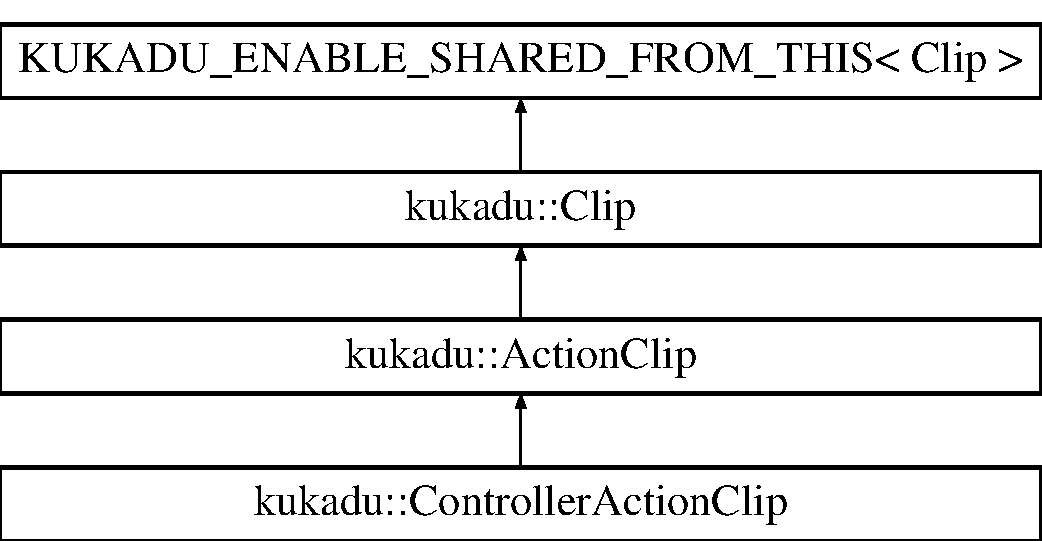
\includegraphics[height=4.000000cm]{classkukadu_1_1ActionClip}
\end{center}
\end{figure}
\subsection*{Public Member Functions}
\begin{DoxyCompactItemize}
\item 
\hypertarget{classkukadu_1_1ActionClip_a573285d8981842eb3bd73ee0eceef975}{{\bfseries Action\-Clip} (int action\-Id, int percept\-Dimensionality, std\-::string label, K\-U\-K\-A\-D\-U\-\_\-\-S\-H\-A\-R\-E\-D\-\_\-\-P\-T\-R$<$ kukadu\-\_\-mersenne\-\_\-twister $>$ generator)}\label{classkukadu_1_1ActionClip_a573285d8981842eb3bd73ee0eceef975}

\item 
\hypertarget{classkukadu_1_1ActionClip_a25f3c4c0f45fc94be915d03231024c25}{int {\bfseries get\-Action\-Id} ()}\label{classkukadu_1_1ActionClip_a25f3c4c0f45fc94be915d03231024c25}

\item 
\hypertarget{classkukadu_1_1ActionClip_a14ec94afcf87bd276f2b3f1c7b9b810f}{std\-::string {\bfseries get\-Label} ()}\label{classkukadu_1_1ActionClip_a14ec94afcf87bd276f2b3f1c7b9b810f}

\item 
\hypertarget{classkukadu_1_1ActionClip_aeff3b2812cc84231eea29f80e6905ff8}{virtual std\-::string {\bfseries to\-String} () const }\label{classkukadu_1_1ActionClip_aeff3b2812cc84231eea29f80e6905ff8}

\item 
\hypertarget{classkukadu_1_1ActionClip_a4c670bb04a291d7dd8ac83d23779b219}{std\-::pair$<$ int, \\*
K\-U\-K\-A\-D\-U\-\_\-\-S\-H\-A\-R\-E\-D\-\_\-\-P\-T\-R$<$ \hyperlink{classkukadu_1_1Clip}{Clip} $>$ $>$ {\bfseries jump\-Next\-Random} ()}\label{classkukadu_1_1ActionClip_a4c670bb04a291d7dd8ac83d23779b219}

\end{DoxyCompactItemize}
\subsection*{Additional Inherited Members}


The documentation for this class was generated from the following files\-:\begin{DoxyCompactItemize}
\item 
/home/c7031109/iis\-\_\-robot\-\_\-sw/iis\-\_\-catkin\-\_\-ws/src/kukadu/include/kukadu/learning/projective\-\_\-simulation/core/actionclip.\-hpp\item 
/home/c7031109/iis\-\_\-robot\-\_\-sw/iis\-\_\-catkin\-\_\-ws/src/kukadu/src/learning/projective\-\_\-simulation/core/actionclip.\-cpp\end{DoxyCompactItemize}

\hypertarget{structkukadu_1_1armacomp}{\section{kukadu\-:\-:armacomp Struct Reference}
\label{structkukadu_1_1armacomp}\index{kukadu\-::armacomp@{kukadu\-::armacomp}}
}
\subsection*{Public Member Functions}
\begin{DoxyCompactItemize}
\item 
\hypertarget{structkukadu_1_1armacomp_ae171e976c645755c8b316d864f778c5e}{int {\bfseries operator()} (const arma\-::vec \&vec1, const arma\-::vec \&vec2) const }\label{structkukadu_1_1armacomp_ae171e976c645755c8b316d864f778c5e}

\end{DoxyCompactItemize}


The documentation for this struct was generated from the following file\-:\begin{DoxyCompactItemize}
\item 
/home/c7031109/iis\-\_\-robot\-\_\-sw/iis\-\_\-catkin\-\_\-ws/src/kukadu/include/kukadu/learning/metric\-\_\-learning/togersonmetriclearner.\-hpp\end{DoxyCompactItemize}

\hypertarget{classkukadu_1_1CartesianDMP}{\section{kukadu\-:\-:Cartesian\-D\-M\-P Class Reference}
\label{classkukadu_1_1CartesianDMP}\index{kukadu\-::\-Cartesian\-D\-M\-P@{kukadu\-::\-Cartesian\-D\-M\-P}}
}
Inheritance diagram for kukadu\-:\-:Cartesian\-D\-M\-P\-:\begin{figure}[H]
\begin{center}
\leavevmode
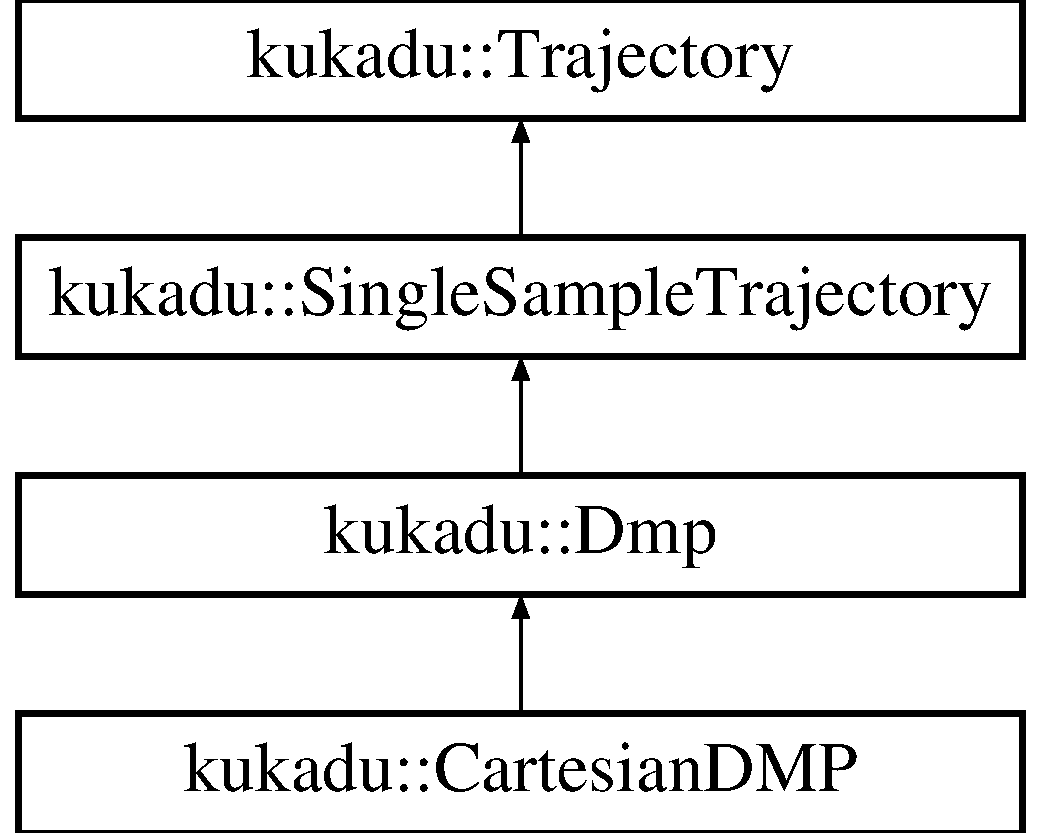
\includegraphics[height=4.000000cm]{classkukadu_1_1CartesianDMP}
\end{center}
\end{figure}
\subsection*{Public Member Functions}
\begin{DoxyCompactItemize}
\item 
\hypertarget{classkukadu_1_1CartesianDMP_a1294c6512ad32f2687b61c04c1081f65}{{\bfseries Cartesian\-D\-M\-P} (arma\-::vec supervised\-Ts, std\-::vector$<$ arma\-::vec $>$ sample\-Ys, std\-::vector$<$ arma\-::vec $>$ fit\-Ys, std\-::vector$<$ arma\-::vec $>$ dmp\-Coeffs, std\-::vector$<$ \hyperlink{classkukadu_1_1DMPBase}{D\-M\-P\-Base} $>$ dmp\-Base, std\-::vector$<$ arma\-::mat $>$ design\-Matrices, double tau, double az, double bz, double ax, double ac, double dmp\-Step\-Size, double tol\-Abs\-Err, double tol\-Rel\-Err)}\label{classkukadu_1_1CartesianDMP_a1294c6512ad32f2687b61c04c1081f65}

\item 
\hypertarget{classkukadu_1_1CartesianDMP_a2618e25d1a5f435ce595c38480cc8dc1}{{\bfseries Cartesian\-D\-M\-P} (arma\-::vec supervised\-Ts, std\-::vector$<$ arma\-::vec $>$ sample\-Ys, std\-::vector$<$ arma\-::vec $>$ fit\-Ys, std\-::vector$<$ arma\-::vec $>$ dmp\-Coeffs, std\-::vector$<$ \hyperlink{classkukadu_1_1DMPBase}{D\-M\-P\-Base} $>$ dmp\-Base, std\-::vector$<$ arma\-::mat $>$ design\-Matrices, double tau, double az, double bz, double ax)}\label{classkukadu_1_1CartesianDMP_a2618e25d1a5f435ce595c38480cc8dc1}

\item 
\hypertarget{classkukadu_1_1CartesianDMP_a997fb24bb6822ffe0dfd9ae6baabf1eb}{{\bfseries Cartesian\-D\-M\-P} (std\-::string dmp\-File)}\label{classkukadu_1_1CartesianDMP_a997fb24bb6822ffe0dfd9ae6baabf1eb}

\item 
\hypertarget{classkukadu_1_1CartesianDMP_a5a34b24a6adb33e88d5850e6d3eaac0d}{bool {\bfseries is\-Cartesian} ()}\label{classkukadu_1_1CartesianDMP_a5a34b24a6adb33e88d5850e6d3eaac0d}

\item 
\hypertarget{classkukadu_1_1CartesianDMP_a705f7a1a000bfa01818272eadd44baaa}{tf\-::\-Quaternion {\bfseries get\-Q0} ()}\label{classkukadu_1_1CartesianDMP_a705f7a1a000bfa01818272eadd44baaa}

\item 
\hypertarget{classkukadu_1_1CartesianDMP_a955ca43e43d62e25dbd765b527fec609}{tf\-::\-Quaternion {\bfseries get\-Qg} ()}\label{classkukadu_1_1CartesianDMP_a955ca43e43d62e25dbd765b527fec609}

\item 
\hypertarget{classkukadu_1_1CartesianDMP_ace0ee0c745d7d3dd6f5d2a04715fc173}{tf\-::\-Quaternion {\bfseries get\-Q\-By\-Idx} (int idx)}\label{classkukadu_1_1CartesianDMP_ace0ee0c745d7d3dd6f5d2a04715fc173}

\item 
\hypertarget{classkukadu_1_1CartesianDMP_a1a973cebbac6ef7039ab1d5a22d56d94}{arma\-::vec {\bfseries get\-Eta0} ()}\label{classkukadu_1_1CartesianDMP_a1a973cebbac6ef7039ab1d5a22d56d94}

\item 
\hypertarget{classkukadu_1_1CartesianDMP_a7d296abeb41ad68cd9b2dd6ca41efd27}{arma\-::vec {\bfseries get\-Eta\-By\-Idx} (int idx)}\label{classkukadu_1_1CartesianDMP_a7d296abeb41ad68cd9b2dd6ca41efd27}

\item 
\hypertarget{classkukadu_1_1CartesianDMP_a9e4074fd82f6256d3b534015c03c3912}{K\-U\-K\-A\-D\-U\-\_\-\-S\-H\-A\-R\-E\-D\-\_\-\-P\-T\-R$<$ \hyperlink{classkukadu_1_1Trajectory}{Trajectory} $>$ {\bfseries copy} ()}\label{classkukadu_1_1CartesianDMP_a9e4074fd82f6256d3b534015c03c3912}

\end{DoxyCompactItemize}
\subsection*{Additional Inherited Members}


The documentation for this class was generated from the following files\-:\begin{DoxyCompactItemize}
\item 
/home/c7031109/iis\-\_\-robot\-\_\-sw/iis\-\_\-catkin\-\_\-ws/src/kukadu/include/kukadu/types/cartesiandmp.\-hpp\item 
/home/c7031109/iis\-\_\-robot\-\_\-sw/iis\-\_\-catkin\-\_\-ws/src/kukadu/src/types/cartesiandmp.\-cpp\end{DoxyCompactItemize}

\hypertarget{classkukadu_1_1CartesianDMPLearner}{\section{kukadu\-:\-:Cartesian\-D\-M\-P\-Learner Class Reference}
\label{classkukadu_1_1CartesianDMPLearner}\index{kukadu\-::\-Cartesian\-D\-M\-P\-Learner@{kukadu\-::\-Cartesian\-D\-M\-P\-Learner}}
}


The Trajectory\-D\-M\-P\-Learner encapsulates the dmp learning process.  




{\ttfamily \#include $<$cartesiandmplearner.\-hpp$>$}

Inheritance diagram for kukadu\-:\-:Cartesian\-D\-M\-P\-Learner\-:\begin{figure}[H]
\begin{center}
\leavevmode
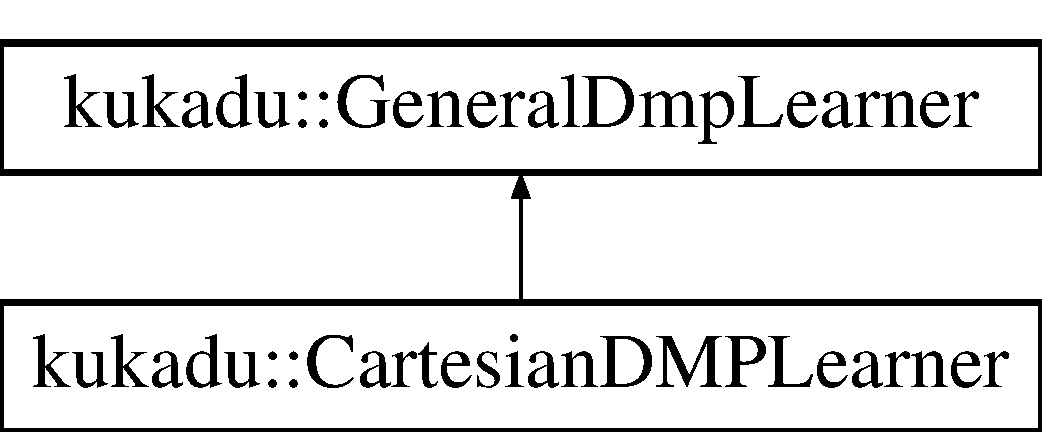
\includegraphics[height=2.000000cm]{classkukadu_1_1CartesianDMPLearner}
\end{center}
\end{figure}
\subsection*{Public Member Functions}
\begin{DoxyCompactItemize}
\item 
\hyperlink{classkukadu_1_1CartesianDMPLearner_a5e1f50a8e9ca6279dec1e797539776e3}{Cartesian\-D\-M\-P\-Learner} (std\-::vector$<$ \hyperlink{classkukadu_1_1DMPBase}{D\-M\-P\-Base} $>$ dmp\-Base, double tau, double az, double bz, double ax, arma\-::mat joints)
\begin{DoxyCompactList}\small\item\em constructor \end{DoxyCompactList}\item 
\hyperlink{classkukadu_1_1CartesianDMPLearner_a827dfdfd4ae5f2052ad67d429a0b10b5}{Cartesian\-D\-M\-P\-Learner} (std\-::vector$<$ double $>$ mys\-Def, std\-::vector$<$ double $>$ sigmas\-Def, double az, double bz, std\-::string file)
\begin{DoxyCompactList}\small\item\em constructor \end{DoxyCompactList}\item 
\hypertarget{classkukadu_1_1CartesianDMPLearner_a7f6c5dd882679d153af81ec8f87e6126}{{\bfseries Cartesian\-D\-M\-P\-Learner} (double az, double bz, std\-::string file)}\label{classkukadu_1_1CartesianDMPLearner_a7f6c5dd882679d153af81ec8f87e6126}

\item 
\hypertarget{classkukadu_1_1CartesianDMPLearner_ab44433d67c81960c8b2083b74b383071}{{\bfseries Cartesian\-D\-M\-P\-Learner} (double az, double bz, arma\-::mat joints)}\label{classkukadu_1_1CartesianDMPLearner_ab44433d67c81960c8b2083b74b383071}

\end{DoxyCompactItemize}
\subsection*{Protected Member Functions}
\begin{DoxyCompactItemize}
\item 
\hypertarget{classkukadu_1_1CartesianDMPLearner_a5e4311236c5bafb415d5c2a410050aee}{K\-U\-K\-A\-D\-U\-\_\-\-S\-H\-A\-R\-E\-D\-\_\-\-P\-T\-R$<$ \hyperlink{classkukadu_1_1Dmp}{Dmp} $>$ {\bfseries create\-Dmp\-Instance} (arma\-::vec supervised\-Ts, std\-::vector$<$ arma\-::vec $>$ sample\-Ys, std\-::vector$<$ arma\-::vec $>$ fit\-Ys, std\-::vector$<$ arma\-::vec $>$ dmp\-Coeffs, std\-::vector$<$ \hyperlink{classkukadu_1_1DMPBase}{D\-M\-P\-Base} $>$ dmp\-Base, std\-::vector$<$ arma\-::mat $>$ design\-Matrices, double tau, double az, double bz, double ax)}\label{classkukadu_1_1CartesianDMPLearner_a5e4311236c5bafb415d5c2a410050aee}

\item 
\hypertarget{classkukadu_1_1CartesianDMPLearner_a17b09095c1a7e462e34bf5448cb021ab}{arma\-::mat {\bfseries compute\-Fit\-Y} (arma\-::vec \&time, arma\-::mat \&y, arma\-::mat \&dy, arma\-::mat \&ddy, arma\-::vec \&vec\-\_\-g)}\label{classkukadu_1_1CartesianDMPLearner_a17b09095c1a7e462e34bf5448cb021ab}

\end{DoxyCompactItemize}
\subsection*{Additional Inherited Members}


\subsection{Detailed Description}
The Trajectory\-D\-M\-P\-Learner encapsulates the dmp learning process. 

Dynamic movement primitives can be easily learned by using this class and providing the joint data or a file containing this data. Basically this is a helper that enables the programmer to reduce code complexity. 

\subsection{Constructor \& Destructor Documentation}
\hypertarget{classkukadu_1_1CartesianDMPLearner_a5e1f50a8e9ca6279dec1e797539776e3}{\index{kukadu\-::\-Cartesian\-D\-M\-P\-Learner@{kukadu\-::\-Cartesian\-D\-M\-P\-Learner}!Cartesian\-D\-M\-P\-Learner@{Cartesian\-D\-M\-P\-Learner}}
\index{Cartesian\-D\-M\-P\-Learner@{Cartesian\-D\-M\-P\-Learner}!kukadu::CartesianDMPLearner@{kukadu\-::\-Cartesian\-D\-M\-P\-Learner}}
\subsubsection[{Cartesian\-D\-M\-P\-Learner}]{\setlength{\rightskip}{0pt plus 5cm}kukadu\-::\-Cartesian\-D\-M\-P\-Learner\-::\-Cartesian\-D\-M\-P\-Learner (
\begin{DoxyParamCaption}
\item[{std\-::vector$<$ {\bf D\-M\-P\-Base} $>$}]{dmp\-Base, }
\item[{double}]{tau, }
\item[{double}]{az, }
\item[{double}]{bz, }
\item[{double}]{ax, }
\item[{arma\-::mat}]{joints}
\end{DoxyParamCaption}
)}}\label{classkukadu_1_1CartesianDMPLearner_a5e1f50a8e9ca6279dec1e797539776e3}


constructor 


\begin{DoxyParams}{Parameters}
{\em dmp\-Base} & dmp basis function definition \\
\hline
{\em tau} & dmp timing constant \\
\hline
{\em az} & dmp az constant \\
\hline
{\em bz} & dmp bz constant \\
\hline
{\em ax} & dmp ax constant \\
\hline
{\em joints} & measured joints \\
\hline
{\em deg\-Freedom} & robots degrees of freedom \\
\hline
\end{DoxyParams}
\hypertarget{classkukadu_1_1CartesianDMPLearner_a827dfdfd4ae5f2052ad67d429a0b10b5}{\index{kukadu\-::\-Cartesian\-D\-M\-P\-Learner@{kukadu\-::\-Cartesian\-D\-M\-P\-Learner}!Cartesian\-D\-M\-P\-Learner@{Cartesian\-D\-M\-P\-Learner}}
\index{Cartesian\-D\-M\-P\-Learner@{Cartesian\-D\-M\-P\-Learner}!kukadu::CartesianDMPLearner@{kukadu\-::\-Cartesian\-D\-M\-P\-Learner}}
\subsubsection[{Cartesian\-D\-M\-P\-Learner}]{\setlength{\rightskip}{0pt plus 5cm}kukadu\-::\-Cartesian\-D\-M\-P\-Learner\-::\-Cartesian\-D\-M\-P\-Learner (
\begin{DoxyParamCaption}
\item[{std\-::vector$<$ double $>$}]{mys\-Def, }
\item[{std\-::vector$<$ double $>$}]{sigmas\-Def, }
\item[{double}]{az, }
\item[{double}]{bz, }
\item[{std\-::string}]{file}
\end{DoxyParamCaption}
)}}\label{classkukadu_1_1CartesianDMPLearner_a827dfdfd4ae5f2052ad67d429a0b10b5}


constructor 


\begin{DoxyParams}{Parameters}
{\em dmp\-Base} & dmp basis function definition \\
\hline
{\em tau} & dmp timing constant \\
\hline
{\em az} & dmp az constant \\
\hline
{\em bz} & dmp bz constant \\
\hline
{\em ax} & dmp ax constant \\
\hline
{\em file} & file containing the measured joints \\
\hline
{\em deg\-Freedom} & robots degrees of freedom \\
\hline
\end{DoxyParams}


The documentation for this class was generated from the following files\-:\begin{DoxyCompactItemize}
\item 
/home/c7031109/iis\-\_\-robot\-\_\-sw/iis\-\_\-catkin\-\_\-ws/src/kukadu/include/kukadu/control/cartesiandmplearner.\-hpp\item 
/home/c7031109/iis\-\_\-robot\-\_\-sw/iis\-\_\-catkin\-\_\-ws/src/kukadu/src/control/cartesiandmplearner.\-cpp\end{DoxyCompactItemize}

\hypertarget{classkukadu_1_1Clip}{\section{kukadu\-:\-:Clip Class Reference}
\label{classkukadu_1_1Clip}\index{kukadu\-::\-Clip@{kukadu\-::\-Clip}}
}
Inheritance diagram for kukadu\-:\-:Clip\-:\begin{figure}[H]
\begin{center}
\leavevmode
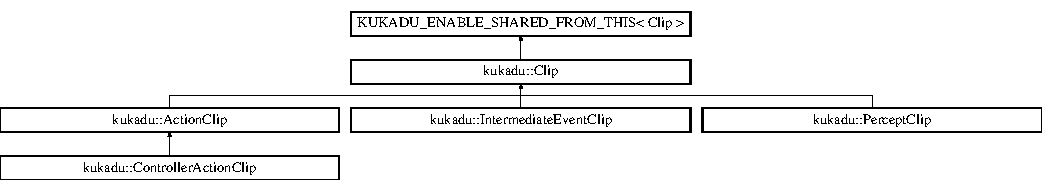
\includegraphics[height=2.424242cm]{classkukadu_1_1Clip}
\end{center}
\end{figure}
\subsection*{Public Member Functions}
\begin{DoxyCompactItemize}
\item 
\hypertarget{classkukadu_1_1Clip_a83a5e4e39bce4974e6b18cee366a67ef}{{\bfseries Clip} (int level, K\-U\-K\-A\-D\-U\-\_\-\-S\-H\-A\-R\-E\-D\-\_\-\-P\-T\-R$<$ kukadu\-\_\-mersenne\-\_\-twister $>$ generator, std\-::string clip\-Values, int immunity)}\label{classkukadu_1_1Clip_a83a5e4e39bce4974e6b18cee366a67ef}

\item 
\hypertarget{classkukadu_1_1Clip_a4ac76920acd4a62b5e5a2ab72dc2c83a}{{\bfseries Clip} (int level, K\-U\-K\-A\-D\-U\-\_\-\-S\-H\-A\-R\-E\-D\-\_\-\-P\-T\-R$<$ kukadu\-\_\-mersenne\-\_\-twister $>$ generator, K\-U\-K\-A\-D\-U\-\_\-\-S\-H\-A\-R\-E\-D\-\_\-\-P\-T\-R$<$ std\-::vector$<$ int $>$ $>$ clip\-Values, int immunity)}\label{classkukadu_1_1Clip_a4ac76920acd4a62b5e5a2ab72dc2c83a}

\item 
\hypertarget{classkukadu_1_1Clip_a6591c7a207c086426e11027419d4f895}{virtual std\-::pair$<$ int, \\*
K\-U\-K\-A\-D\-U\-\_\-\-S\-H\-A\-R\-E\-D\-\_\-\-P\-T\-R$<$ \hyperlink{classkukadu_1_1Clip}{Clip} $>$ $>$ {\bfseries jump\-Next\-Random} ()}\label{classkukadu_1_1Clip_a6591c7a207c086426e11027419d4f895}

\item 
\hypertarget{classkukadu_1_1Clip_a4c58b4758a6b673bd26ce3afbeb1f259}{void {\bfseries print\-Sub\-Weights} ()}\label{classkukadu_1_1Clip_a4c58b4758a6b673bd26ce3afbeb1f259}

\item 
\hypertarget{classkukadu_1_1Clip_ab63c6f4922b2e61d5caedae2ab4e9566}{void {\bfseries set\-Previous\-Rank} ()}\label{classkukadu_1_1Clip_ab63c6f4922b2e61d5caedae2ab4e9566}

\item 
\hypertarget{classkukadu_1_1Clip_a3d532729bf05cebcfcf049be5c15383b}{void {\bfseries decrease\-Immunity} ()}\label{classkukadu_1_1Clip_a3d532729bf05cebcfcf049be5c15383b}

\item 
\hypertarget{classkukadu_1_1Clip_a72e5e78f3bdc0f80c32e4775e37d4b04}{void {\bfseries remove\-All\-Sub\-Clips} ()}\label{classkukadu_1_1Clip_a72e5e78f3bdc0f80c32e4775e37d4b04}

\item 
\hypertarget{classkukadu_1_1Clip_a5cfdcf67876c3856b65f6bceb07a0cfd}{void {\bfseries init\-Random\-Generator} ()}\label{classkukadu_1_1Clip_a5cfdcf67876c3856b65f6bceb07a0cfd}

\item 
\hypertarget{classkukadu_1_1Clip_ab31cf5283dab670017ae01e5ebf35afb}{void {\bfseries set\-Immunity} (int immunity)}\label{classkukadu_1_1Clip_ab31cf5283dab670017ae01e5ebf35afb}

\item 
\hypertarget{classkukadu_1_1Clip_a9f8015a0b15359f9ce5101cfa01954ba}{void {\bfseries add\-Parent} (K\-U\-K\-A\-D\-U\-\_\-\-S\-H\-A\-R\-E\-D\-\_\-\-P\-T\-R$<$ \hyperlink{classkukadu_1_1Clip}{Clip} $>$ par)}\label{classkukadu_1_1Clip_a9f8015a0b15359f9ce5101cfa01954ba}

\item 
\hypertarget{classkukadu_1_1Clip_a79f9730aaded88c922fc1693582b62e0}{void {\bfseries add\-H\-And\-Initialize} (int idx, int add\-Weight)}\label{classkukadu_1_1Clip_a79f9730aaded88c922fc1693582b62e0}

\item 
\hypertarget{classkukadu_1_1Clip_a6845f2bed6e81c012c3475e0497b0448}{void {\bfseries update\-Weights} (double reward, double gamma)}\label{classkukadu_1_1Clip_a6845f2bed6e81c012c3475e0497b0448}

\item 
\hypertarget{classkukadu_1_1Clip_a95eee9c3a13b7b202bfdf6d4b29603d9}{void {\bfseries remove\-Sub\-Clip} (K\-U\-K\-A\-D\-U\-\_\-\-S\-H\-A\-R\-E\-D\-\_\-\-P\-T\-R$<$ \hyperlink{classkukadu_1_1Clip}{Clip} $>$ clip)}\label{classkukadu_1_1Clip_a95eee9c3a13b7b202bfdf6d4b29603d9}

\item 
\hypertarget{classkukadu_1_1Clip_a3d65cf6aadee55889068d9734ab4b9b9}{void {\bfseries remove\-Parent\-Clip} (K\-U\-K\-A\-D\-U\-\_\-\-S\-H\-A\-R\-E\-D\-\_\-\-P\-T\-R$<$ \hyperlink{classkukadu_1_1Clip}{Clip} $>$ c)}\label{classkukadu_1_1Clip_a3d65cf6aadee55889068d9734ab4b9b9}

\item 
\hypertarget{classkukadu_1_1Clip_a5cd572f564c87baaef107e88f0097d57}{void {\bfseries add\-Child\-Upwards} (K\-U\-K\-A\-D\-U\-\_\-\-S\-H\-A\-R\-E\-D\-\_\-\-P\-T\-R$<$ \hyperlink{classkukadu_1_1Clip}{Clip} $>$ sub)}\label{classkukadu_1_1Clip_a5cd572f564c87baaef107e88f0097d57}

\item 
\hypertarget{classkukadu_1_1Clip_a6183ebd44f8c20e2b588e0d85c616c34}{void {\bfseries add\-Parent\-Downwards} (K\-U\-K\-A\-D\-U\-\_\-\-S\-H\-A\-R\-E\-D\-\_\-\-P\-T\-R$<$ \hyperlink{classkukadu_1_1Clip}{Clip} $>$ par)}\label{classkukadu_1_1Clip_a6183ebd44f8c20e2b588e0d85c616c34}

\item 
\hypertarget{classkukadu_1_1Clip_afc489cc62a302b2a679374b4617e5a31}{void {\bfseries remove\-Sub\-Clip\-Wo\-Rand} (K\-U\-K\-A\-D\-U\-\_\-\-S\-H\-A\-R\-E\-D\-\_\-\-P\-T\-R$<$ \hyperlink{classkukadu_1_1Clip}{Clip} $>$ clip)}\label{classkukadu_1_1Clip_afc489cc62a302b2a679374b4617e5a31}

\item 
\hypertarget{classkukadu_1_1Clip_a2247e017be36476075ce9ce68358e53d}{void {\bfseries add\-Sub\-Clip} (K\-U\-K\-A\-D\-U\-\_\-\-S\-H\-A\-R\-E\-D\-\_\-\-P\-T\-R$<$ \hyperlink{classkukadu_1_1Clip}{Clip} $>$ sub, int weight)}\label{classkukadu_1_1Clip_a2247e017be36476075ce9ce68358e53d}

\item 
\hypertarget{classkukadu_1_1Clip_af56ce79b2094de5bcab46642bad5d817}{void {\bfseries set\-Clip\-Dimension\-Values} (K\-U\-K\-A\-D\-U\-\_\-\-S\-H\-A\-R\-E\-D\-\_\-\-P\-T\-R$<$ std\-::vector$<$ int $>$ $>$ vals)}\label{classkukadu_1_1Clip_af56ce79b2094de5bcab46642bad5d817}

\item 
\hypertarget{classkukadu_1_1Clip_a088ed28a35cf7c00f4fff1fa62936cd0}{void {\bfseries set\-Children} (K\-U\-K\-A\-D\-U\-\_\-\-S\-H\-A\-R\-E\-D\-\_\-\-P\-T\-R$<$ std\-::vector$<$ K\-U\-K\-A\-D\-U\-\_\-\-S\-H\-A\-R\-E\-D\-\_\-\-P\-T\-R$<$ \hyperlink{classkukadu_1_1Clip}{Clip} $>$ $>$ $>$ children)}\label{classkukadu_1_1Clip_a088ed28a35cf7c00f4fff1fa62936cd0}

\item 
\hypertarget{classkukadu_1_1Clip_aaf2e88408e9b5d7001ca8563b8a1abdf}{void {\bfseries set\-Children} (K\-U\-K\-A\-D\-U\-\_\-\-S\-H\-A\-R\-E\-D\-\_\-\-P\-T\-R$<$ std\-::vector$<$ K\-U\-K\-A\-D\-U\-\_\-\-S\-H\-A\-R\-E\-D\-\_\-\-P\-T\-R$<$ \hyperlink{classkukadu_1_1Clip}{Clip} $>$ $>$ $>$ children, std\-::vector$<$ double $>$ weights)}\label{classkukadu_1_1Clip_aaf2e88408e9b5d7001ca8563b8a1abdf}

\item 
\hypertarget{classkukadu_1_1Clip_a3f1ecbecfc7d21c19e12ccfcafdad8f6}{bool {\bfseries is\-Immune} ()}\label{classkukadu_1_1Clip_a3f1ecbecfc7d21c19e12ccfcafdad8f6}

\item 
\hypertarget{classkukadu_1_1Clip_a13473decc67ef399684148824adc087c}{virtual bool {\bfseries is\-Compatible\-Subclip} (K\-U\-K\-A\-D\-U\-\_\-\-S\-H\-A\-R\-E\-D\-\_\-\-P\-T\-R$<$ \hyperlink{classkukadu_1_1Clip}{Clip} $>$ c)}\label{classkukadu_1_1Clip_a13473decc67ef399684148824adc087c}

\item 
\hypertarget{classkukadu_1_1Clip_ab1db78313a620ad816b9225e26bcedfe}{int {\bfseries get\-Level} ()}\label{classkukadu_1_1Clip_ab1db78313a620ad816b9225e26bcedfe}

\item 
\hypertarget{classkukadu_1_1Clip_a0588408a7fef34c3503f3c5236ea01f7}{int {\bfseries get\-Previous\-Rank} ()}\label{classkukadu_1_1Clip_a0588408a7fef34c3503f3c5236ea01f7}

\item 
\hypertarget{classkukadu_1_1Clip_af77cf93b544392ef68a2cb036073bb5c}{int {\bfseries get\-Sub\-Clip\-Count} ()}\label{classkukadu_1_1Clip_af77cf93b544392ef68a2cb036073bb5c}

\item 
\hypertarget{classkukadu_1_1Clip_abc2dd87e529d55767e168f8cc5544d51}{int {\bfseries get\-Dimensionality} ()}\label{classkukadu_1_1Clip_abc2dd87e529d55767e168f8cc5544d51}

\item 
\hypertarget{classkukadu_1_1Clip_a529397c2adfe87b4d71ff48941e9606e}{int {\bfseries get\-Initial\-Immunity} ()}\label{classkukadu_1_1Clip_a529397c2adfe87b4d71ff48941e9606e}

\item 
\hypertarget{classkukadu_1_1Clip_a70b0e249985d664605320bb8bc58b246}{int {\bfseries get\-Current\-Immunity} ()}\label{classkukadu_1_1Clip_a70b0e249985d664605320bb8bc58b246}

\item 
\hypertarget{classkukadu_1_1Clip_a47e51b76f2308a7775d9b6ceb92231a5}{int {\bfseries get\-Sub\-Clip\-Idx} (K\-U\-K\-A\-D\-U\-\_\-\-S\-H\-A\-R\-E\-D\-\_\-\-P\-T\-R$<$ \hyperlink{classkukadu_1_1Clip}{Clip} $>$ sub\-Clip)}\label{classkukadu_1_1Clip_a47e51b76f2308a7775d9b6ceb92231a5}

\item 
\hypertarget{classkukadu_1_1Clip_ae79760b863e5c56cef78a137243c33f4}{double {\bfseries get\-Weight\-By\-Idx} (int idx)}\label{classkukadu_1_1Clip_ae79760b863e5c56cef78a137243c33f4}

\item 
\hypertarget{classkukadu_1_1Clip_a05ab9806e99f04e02b8af71a5130a6bb}{double {\bfseries compute\-Sub\-Entropy} () const }\label{classkukadu_1_1Clip_a05ab9806e99f04e02b8af71a5130a6bb}

\item 
\hypertarget{classkukadu_1_1Clip_ab6d3da091cd55f6e85abf03fa31d4eac}{virtual double {\bfseries compute\-Rank} () const }\label{classkukadu_1_1Clip_ab6d3da091cd55f6e85abf03fa31d4eac}

\item 
\hypertarget{classkukadu_1_1Clip_a0e794578f3fcb41fd6dd499c22c30565}{std\-::string {\bfseries get\-Id\-Vec\-String} () const }\label{classkukadu_1_1Clip_a0e794578f3fcb41fd6dd499c22c30565}

\item 
\hypertarget{classkukadu_1_1Clip_abf1bb19d4b0094d616f543120dedbd7d}{virtual std\-::string {\bfseries to\-String} () const }\label{classkukadu_1_1Clip_abf1bb19d4b0094d616f543120dedbd7d}

\item 
\hypertarget{classkukadu_1_1Clip_a6b905b49fbab541a181a6883da7a868a}{void {\bfseries set\-Next\-Hop} (int hop\-Idx)}\label{classkukadu_1_1Clip_a6b905b49fbab541a181a6883da7a868a}

\item 
\hypertarget{classkukadu_1_1Clip_a0d4f9f3ecb5df4734e3d46a98a237ee7}{void {\bfseries set\-Next\-Hop} (K\-U\-K\-A\-D\-U\-\_\-\-S\-H\-A\-R\-E\-D\-\_\-\-P\-T\-R$<$ \hyperlink{classkukadu_1_1Clip}{Clip} $>$ hop\-Clip)}\label{classkukadu_1_1Clip_a0d4f9f3ecb5df4734e3d46a98a237ee7}

\item 
\hypertarget{classkukadu_1_1Clip_acdfec2bfb4968418b9b24696af6b07a6}{K\-U\-K\-A\-D\-U\-\_\-\-S\-H\-A\-R\-E\-D\-\_\-\-P\-T\-R$<$ std\-::vector\\*
$<$ K\-U\-K\-A\-D\-U\-\_\-\-S\-H\-A\-R\-E\-D\-\_\-\-P\-T\-R$<$ \hyperlink{classkukadu_1_1Clip}{Clip} $>$ $>$ $>$ {\bfseries get\-Sub\-Clips} ()}\label{classkukadu_1_1Clip_acdfec2bfb4968418b9b24696af6b07a6}

\item 
\hypertarget{classkukadu_1_1Clip_ab6089133084f49019e2fd6e6373c67e8}{K\-U\-K\-A\-D\-U\-\_\-\-S\-H\-A\-R\-E\-D\-\_\-\-P\-T\-R$<$ \hyperlink{classkukadu_1_1Clip}{Clip} $>$ {\bfseries get\-Likeliest\-Child} ()}\label{classkukadu_1_1Clip_ab6089133084f49019e2fd6e6373c67e8}

\item 
\hypertarget{classkukadu_1_1Clip_a97677251b01b02c3b4800d04ca6ad07e}{K\-U\-K\-A\-D\-U\-\_\-\-S\-H\-A\-R\-E\-D\-\_\-\-P\-T\-R$<$ \hyperlink{classkukadu_1_1Clip}{Clip} $>$ {\bfseries get\-Sub\-Clip\-By\-Idx} (int idx)}\label{classkukadu_1_1Clip_a97677251b01b02c3b4800d04ca6ad07e}

\item 
\hypertarget{classkukadu_1_1Clip_af046e5a1afee00613e11fcb2e48d28fc}{K\-U\-K\-A\-D\-U\-\_\-\-S\-H\-A\-R\-E\-D\-\_\-\-P\-T\-R$<$ \hyperlink{classkukadu_1_1Clip}{Clip} $>$ {\bfseries get\-Sub\-Clip\-By\-Label} (std\-::string idx)}\label{classkukadu_1_1Clip_af046e5a1afee00613e11fcb2e48d28fc}

\item 
\hypertarget{classkukadu_1_1Clip_ad68e8835167a1bd4197819891f3114e5}{K\-U\-K\-A\-D\-U\-\_\-\-S\-H\-A\-R\-E\-D\-\_\-\-P\-T\-R$<$ std\-::vector\\*
$<$ int $>$ $>$ {\bfseries get\-Clip\-Dimensions} () const }\label{classkukadu_1_1Clip_ad68e8835167a1bd4197819891f3114e5}

\item 
\hypertarget{classkukadu_1_1Clip_a31c64a7290c936dc63b48b47ba563297}{K\-U\-K\-A\-D\-U\-\_\-\-S\-H\-A\-R\-E\-D\-\_\-\-P\-T\-R$<$ \hyperlink{classkukadu_1_1Clip}{Clip} $>$ {\bfseries compare\-Clip} (K\-U\-K\-A\-D\-U\-\_\-\-S\-H\-A\-R\-E\-D\-\_\-\-P\-T\-R$<$ \hyperlink{classkukadu_1_1Clip}{Clip} $>$ c)}\label{classkukadu_1_1Clip_a31c64a7290c936dc63b48b47ba563297}

\item 
\hypertarget{classkukadu_1_1Clip_aac76795ec89a39adb9b02a7b87f27cb9}{K\-U\-K\-A\-D\-U\-\_\-\-S\-H\-A\-R\-E\-D\-\_\-\-P\-T\-R$<$ std\-::set\\*
$<$ K\-U\-K\-A\-D\-U\-\_\-\-S\-H\-A\-R\-E\-D\-\_\-\-P\-T\-R$<$ \hyperlink{classkukadu_1_1Clip}{Clip} $>$ $>$ $>$ {\bfseries get\-Parents} ()}\label{classkukadu_1_1Clip_aac76795ec89a39adb9b02a7b87f27cb9}

\end{DoxyCompactItemize}
\subsection*{Static Public Member Functions}
\begin{DoxyCompactItemize}
\item 
\hypertarget{classkukadu_1_1Clip_a4aeb1954ae45ed377d3563c79f083329}{static K\-U\-K\-A\-D\-U\-\_\-\-S\-H\-A\-R\-E\-D\-\_\-\-P\-T\-R\\*
$<$ std\-::vector$<$ int $>$ $>$ {\bfseries get\-Id\-Vector\-From\-String} (std\-::string str)}\label{classkukadu_1_1Clip_a4aeb1954ae45ed377d3563c79f083329}

\item 
\hypertarget{classkukadu_1_1Clip_aa8186f0de64ebc0a45c502619c38b020}{static bool {\bfseries compare\-Id\-Vecs} (const K\-U\-K\-A\-D\-U\-\_\-\-S\-H\-A\-R\-E\-D\-\_\-\-P\-T\-R$<$ std\-::vector$<$ int $>$ $>$ vec1, const K\-U\-K\-A\-D\-U\-\_\-\-S\-H\-A\-R\-E\-D\-\_\-\-P\-T\-R$<$ std\-::vector$<$ int $>$ $>$ vec2)}\label{classkukadu_1_1Clip_aa8186f0de64ebc0a45c502619c38b020}

\end{DoxyCompactItemize}
\subsection*{Static Public Attributes}
\begin{DoxyCompactItemize}
\item 
\hypertarget{classkukadu_1_1Clip_a52b125d5ca75e6c980c4efb63e18ae4e}{static const int {\bfseries C\-L\-I\-P\-\_\-\-H\-\_\-\-S\-T\-D\-\_\-\-W\-E\-I\-G\-H\-T} = 1}\label{classkukadu_1_1Clip_a52b125d5ca75e6c980c4efb63e18ae4e}

\item 
\hypertarget{classkukadu_1_1Clip_aaf7152d14703b47492d656333809e38b}{static const int {\bfseries C\-L\-I\-P\-\_\-\-H\-\_\-\-H\-A\-S\-H\-\_\-\-V\-A\-L} = I\-N\-T\-\_\-\-M\-I\-N}\label{classkukadu_1_1Clip_aaf7152d14703b47492d656333809e38b}

\item 
\hypertarget{classkukadu_1_1Clip_a64b769588ddb7d317b0cd6de62c997d2}{static const int {\bfseries C\-L\-I\-P\-\_\-\-H\-\_\-\-L\-E\-V\-E\-L\-\_\-\-F\-I\-N\-A\-L} = -\/1}\label{classkukadu_1_1Clip_a64b769588ddb7d317b0cd6de62c997d2}

\item 
\hypertarget{classkukadu_1_1Clip_acecc38ad6aa9ffdb51d8f44ee8539b9e}{static const int {\bfseries C\-L\-I\-P\-\_\-\-H\-\_\-\-N\-O\-T\-\_\-\-W\-A\-L\-K\-E\-D\-\_\-\-Y\-E\-T} = -\/1}\label{classkukadu_1_1Clip_acecc38ad6aa9ffdb51d8f44ee8539b9e}

\item 
\hypertarget{classkukadu_1_1Clip_a70bbff7bc51184fe67545ce050590bce}{static const int {\bfseries P\-S\-\_\-\-D\-E\-F\-A\-U\-L\-T\-\_\-\-I\-M\-M\-U\-N\-I\-T\-Y} = 1000}\label{classkukadu_1_1Clip_a70bbff7bc51184fe67545ce050590bce}

\end{DoxyCompactItemize}
\subsection*{Protected Attributes}
\begin{DoxyCompactItemize}
\item 
\hypertarget{classkukadu_1_1Clip_a17bb4754cdf923cc3b3c9bc344ec9452}{int {\bfseries visited\-Sub\-Node}}\label{classkukadu_1_1Clip_a17bb4754cdf923cc3b3c9bc344ec9452}

\end{DoxyCompactItemize}
\subsection*{Friends}
\begin{DoxyCompactItemize}
\item 
\hypertarget{classkukadu_1_1Clip_afa49def0694b1872fe61d573e16d05b5}{bool {\bfseries operator$<$} (const \hyperlink{classkukadu_1_1Clip}{Clip} \&o1, const \hyperlink{classkukadu_1_1Clip}{Clip} \&o2)}\label{classkukadu_1_1Clip_afa49def0694b1872fe61d573e16d05b5}

\item 
\hypertarget{classkukadu_1_1Clip_a72090efb6ab8a7595cab10f6d925abd4}{bool {\bfseries operator==} (const \hyperlink{classkukadu_1_1Clip}{Clip} \&o1, const \hyperlink{classkukadu_1_1Clip}{Clip} \&o2)}\label{classkukadu_1_1Clip_a72090efb6ab8a7595cab10f6d925abd4}

\item 
\hypertarget{classkukadu_1_1Clip_a6e577ddd795af4bf2cfe74ea14c3b7bc}{bool {\bfseries operator!=} (const \hyperlink{classkukadu_1_1Clip}{Clip} \&o1, const \hyperlink{classkukadu_1_1Clip}{Clip} \&o2)}\label{classkukadu_1_1Clip_a6e577ddd795af4bf2cfe74ea14c3b7bc}

\item 
\hypertarget{classkukadu_1_1Clip_a01b9c25753a11dcefcbfc0827f876444}{std\-::ostream \& {\bfseries operator$<$$<$} (std\-::ostream \&strm, const \hyperlink{classkukadu_1_1Clip}{Clip} \&c)}\label{classkukadu_1_1Clip_a01b9c25753a11dcefcbfc0827f876444}

\end{DoxyCompactItemize}


The documentation for this class was generated from the following files\-:\begin{DoxyCompactItemize}
\item 
/home/c7031109/iis\-\_\-robot\-\_\-sw/iis\-\_\-catkin\-\_\-ws/src/kukadu/include/kukadu/learning/projective\-\_\-simulation/core/clip.\-hpp\item 
/home/c7031109/iis\-\_\-robot\-\_\-sw/iis\-\_\-catkin\-\_\-ws/src/kukadu/src/learning/projective\-\_\-simulation/core/clip.\-cpp\end{DoxyCompactItemize}

\hypertarget{structkukadu_1_1clip__compare}{\section{kukadu\-:\-:clip\-\_\-compare Struct Reference}
\label{structkukadu_1_1clip__compare}\index{kukadu\-::clip\-\_\-compare@{kukadu\-::clip\-\_\-compare}}
}
\subsection*{Public Member Functions}
\begin{DoxyCompactItemize}
\item 
\hypertarget{structkukadu_1_1clip__compare_a00cb7898ad240af31cf9ca301ae7b7ad}{bool {\bfseries operator()} (K\-U\-K\-A\-D\-U\-\_\-\-S\-H\-A\-R\-E\-D\-\_\-\-P\-T\-R$<$ \hyperlink{classkukadu_1_1Clip}{Clip} $>$ const \&lhs, K\-U\-K\-A\-D\-U\-\_\-\-S\-H\-A\-R\-E\-D\-\_\-\-P\-T\-R$<$ \hyperlink{classkukadu_1_1Clip}{Clip} $>$ const \&rhs)}\label{structkukadu_1_1clip__compare_a00cb7898ad240af31cf9ca301ae7b7ad}

\end{DoxyCompactItemize}


The documentation for this struct was generated from the following file\-:\begin{DoxyCompactItemize}
\item 
/home/c7031109/iis\-\_\-robot\-\_\-sw/iis\-\_\-catkin\-\_\-ws/src/kukadu/include/kukadu/learning/projective\-\_\-simulation/core/projectivesimulator.\-hpp\end{DoxyCompactItemize}

\hypertarget{classkukadu_1_1Clusters}{\section{kukadu\-:\-:Clusters Class Reference}
\label{classkukadu_1_1Clusters}\index{kukadu\-::\-Clusters@{kukadu\-::\-Clusters}}
}
\subsection*{Public Member Functions}
\begin{DoxyCompactItemize}
\item 
\hypertarget{classkukadu_1_1Clusters_ad51562cbdd79886e320e3bd135e09fa7}{{\bfseries Clusters} (Cluster\-Id num\-\_\-clusters, \hyperlink{classkukadu_1_1PointsSpace}{Points\-Space} \&ps)}\label{classkukadu_1_1Clusters_ad51562cbdd79886e320e3bd135e09fa7}

\item 
\hypertarget{classkukadu_1_1Clusters_abbecb3ad5bb32ceeea328b71cd63264c}{void {\bfseries k\-\_\-means} (void)}\label{classkukadu_1_1Clusters_abbecb3ad5bb32ceeea328b71cd63264c}

\end{DoxyCompactItemize}
\subsection*{Friends}
\begin{DoxyCompactItemize}
\item 
\hypertarget{classkukadu_1_1Clusters_a0cd1d4240f35d52f39b3d3ac51be49b8}{std\-::ostream \& {\bfseries operator$<$$<$} (std\-::ostream \&os, \hyperlink{classkukadu_1_1Clusters}{Clusters} \&cl)}\label{classkukadu_1_1Clusters_a0cd1d4240f35d52f39b3d3ac51be49b8}

\end{DoxyCompactItemize}


The documentation for this class was generated from the following files\-:\begin{DoxyCompactItemize}
\item 
/home/c7031109/iis\-\_\-robot\-\_\-sw/iis\-\_\-catkin\-\_\-ws/src/kukadu/include/kukadu/learning/clustering/kmeans.\-hpp\item 
/home/c7031109/iis\-\_\-robot\-\_\-sw/iis\-\_\-catkin\-\_\-ws/src/kukadu/src/learning/clustering/kmeans.\-cpp\end{DoxyCompactItemize}

\hypertarget{classkukadu_1_1ComplexController}{\section{kukadu\-:\-:Complex\-Controller Class Reference}
\label{classkukadu_1_1ComplexController}\index{kukadu\-::\-Complex\-Controller@{kukadu\-::\-Complex\-Controller}}
}
Inheritance diagram for kukadu\-:\-:Complex\-Controller\-:\begin{figure}[H]
\begin{center}
\leavevmode
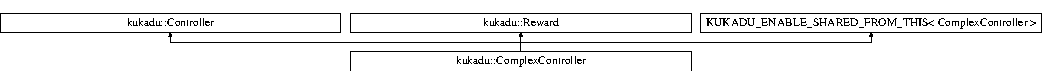
\includegraphics[height=0.957265cm]{classkukadu_1_1ComplexController}
\end{center}
\end{figure}
\subsection*{Public Member Functions}
\begin{DoxyCompactItemize}
\item 
\hypertarget{classkukadu_1_1ComplexController_aaf2e3c2cd9221fb38090d9bf3b26ac43}{{\bfseries Complex\-Controller} (std\-::string caption, std\-::string store\-Path, bool store\-Reward, double sense\-Stretch, double boredom, K\-U\-K\-A\-D\-U\-\_\-\-S\-H\-A\-R\-E\-D\-\_\-\-P\-T\-R$<$ kukadu\-\_\-mersenne\-\_\-twister $>$ generator, int std\-Reward, double punish\-Reward, double gamma, int std\-Prep\-Weight, bool collect\-Prev\-Rewards, int simulation\-Failing\-Probability, int max\-Env\-Path\-Length=4, double path\-Length\-Cost=0.\-01, double std\-Environment\-Reward=10.\-0)}\label{classkukadu_1_1ComplexController_aaf2e3c2cd9221fb38090d9bf3b26ac43}

\item 
\hypertarget{classkukadu_1_1ComplexController_ad79530c882119d956bb0d34669a2f4da}{void {\bfseries store} ()}\label{classkukadu_1_1ComplexController_ad79530c882119d956bb0d34669a2f4da}

\item 
\hypertarget{classkukadu_1_1ComplexController_ab2fc3490e103e0a884b767e9c34cea31}{void {\bfseries load} (std\-::string path, std\-::map$<$ std\-::string, K\-U\-K\-A\-D\-U\-\_\-\-S\-H\-A\-R\-E\-D\-\_\-\-P\-T\-R$<$ \hyperlink{classkukadu_1_1SensingController}{kukadu\-::\-Sensing\-Controller} $>$ $>$ available\-Sensing\-Controllers, std\-::map$<$ std\-::string, K\-U\-K\-A\-D\-U\-\_\-\-S\-H\-A\-R\-E\-D\-\_\-\-P\-T\-R$<$ \hyperlink{classkukadu_1_1Controller}{kukadu\-::\-Controller} $>$ $>$ available\-Preparatory\-Controllers)}\label{classkukadu_1_1ComplexController_ab2fc3490e103e0a884b767e9c34cea31}

\item 
\hypertarget{classkukadu_1_1ComplexController_a22593ed34bf58ee205ddab925bc0d03f}{virtual void {\bfseries initialize} ()}\label{classkukadu_1_1ComplexController_a22593ed34bf58ee205ddab925bc0d03f}

\item 
\hypertarget{classkukadu_1_1ComplexController_a13563bd973c9270984971638484df98d}{void {\bfseries store\-Next\-Iteration} ()}\label{classkukadu_1_1ComplexController_a13563bd973c9270984971638484df98d}

\item 
\hypertarget{classkukadu_1_1ComplexController_a3ebd8d88dc147461fbec6075478b4f7e}{void {\bfseries create\-Sensing\-Database} ()}\label{classkukadu_1_1ComplexController_a3ebd8d88dc147461fbec6075478b4f7e}

\item 
\hypertarget{classkukadu_1_1ComplexController_ae04169f9dcb3970089bb44c8905bcdc4}{void {\bfseries set\-Boredom} (double boredom)}\label{classkukadu_1_1ComplexController_ae04169f9dcb3970089bb44c8905bcdc4}

\item 
\hypertarget{classkukadu_1_1ComplexController_a921fd27f700ee3ff2611546b63f23100}{void {\bfseries store} (std\-::string destination)}\label{classkukadu_1_1ComplexController_a921fd27f700ee3ff2611546b63f23100}

\item 
\hypertarget{classkukadu_1_1ComplexController_a5a0486739a34120b94901f4893fdf8d0}{void {\bfseries set\-Training\-Mode} (bool do\-Training)}\label{classkukadu_1_1ComplexController_a5a0486739a34120b94901f4893fdf8d0}

\item 
\hypertarget{classkukadu_1_1ComplexController_a1481c37be379f4dc717740c6f2bf74a3}{void {\bfseries create\-Sensing\-Database} (std\-::vector$<$ K\-U\-K\-A\-D\-U\-\_\-\-S\-H\-A\-R\-E\-D\-\_\-\-P\-T\-R$<$ \hyperlink{classkukadu_1_1SensingController}{Sensing\-Controller} $>$ $>$ sensing\-Controllers)}\label{classkukadu_1_1ComplexController_a1481c37be379f4dc717740c6f2bf74a3}

\item 
\hypertarget{classkukadu_1_1ComplexController_a43f98dafcffca0e3d437a3dca761ddaf}{void {\bfseries set\-Sensing\-Controllers} (std\-::vector$<$ K\-U\-K\-A\-D\-U\-\_\-\-S\-H\-A\-R\-E\-D\-\_\-\-P\-T\-R$<$ \hyperlink{classkukadu_1_1SensingController}{kukadu\-::\-Sensing\-Controller} $>$ $>$ sensing\-Controllers)}\label{classkukadu_1_1ComplexController_a43f98dafcffca0e3d437a3dca761ddaf}

\item 
\hypertarget{classkukadu_1_1ComplexController_a3221ce22a7472721add0a585e4de12b8}{void {\bfseries set\-Preparatory\-Controllers} (std\-::vector$<$ K\-U\-K\-A\-D\-U\-\_\-\-S\-H\-A\-R\-E\-D\-\_\-\-P\-T\-R$<$ \hyperlink{classkukadu_1_1Controller}{kukadu\-::\-Controller} $>$ $>$ preparatory\-Controllers)}\label{classkukadu_1_1ComplexController_a3221ce22a7472721add0a585e4de12b8}

\item 
\hypertarget{classkukadu_1_1ComplexController_a5c9e2b9e0e9eb58eef8a8b9eceebcb7f}{void {\bfseries clear\-Preparatory\-Controllers} ()}\label{classkukadu_1_1ComplexController_a5c9e2b9e0e9eb58eef8a8b9eceebcb7f}

\item 
\hypertarget{classkukadu_1_1ComplexController_ad432f3b834ecbaba5b47604a695705a6}{void {\bfseries add\-Preparatory\-Controller} (K\-U\-K\-A\-D\-U\-\_\-\-S\-H\-A\-R\-E\-D\-\_\-\-P\-T\-R$<$ \hyperlink{classkukadu_1_1Controller}{kukadu\-::\-Controller} $>$ prep\-Cont)}\label{classkukadu_1_1ComplexController_ad432f3b834ecbaba5b47604a695705a6}

\item 
\hypertarget{classkukadu_1_1ComplexController_a246a72860c5c317173d1f212ac7a25b3}{virtual void {\bfseries execute\-Complex\-Action} ()=0}\label{classkukadu_1_1ComplexController_a246a72860c5c317173d1f212ac7a25b3}

\item 
\hypertarget{classkukadu_1_1ComplexController_abc9b91acb5e94cbc6a4edd1ba3a38583}{int {\bfseries get\-Dimensionality} ()}\label{classkukadu_1_1ComplexController_abc9b91acb5e94cbc6a4edd1ba3a38583}

\item 
\hypertarget{classkukadu_1_1ComplexController_a1b272529d7f87ba1bfe9fde5e99f98de}{virtual int {\bfseries get\-Next\-Simulated\-Ground\-Truth} (K\-U\-K\-A\-D\-U\-\_\-\-S\-H\-A\-R\-E\-D\-\_\-\-P\-T\-R$<$ \hyperlink{classkukadu_1_1SensingController}{Sensing\-Controller} $>$ sens\-Cont)}\label{classkukadu_1_1ComplexController_a1b272529d7f87ba1bfe9fde5e99f98de}

\item 
\hypertarget{classkukadu_1_1ComplexController_a5b8c6fcde91e49e365ada1793f029170}{virtual K\-U\-K\-A\-D\-U\-\_\-\-S\-H\-A\-R\-E\-D\-\_\-\-P\-T\-R$<$ \hyperlink{classkukadu_1_1Clip}{Clip} $>$ {\bfseries compute\-Ground\-Truth\-Transition} (K\-U\-K\-A\-D\-U\-\_\-\-S\-H\-A\-R\-E\-D\-\_\-\-P\-T\-R$<$ \hyperlink{classkukadu_1_1Clip}{Clip} $>$ sensing\-Clip, K\-U\-K\-A\-D\-U\-\_\-\-S\-H\-A\-R\-E\-D\-\_\-\-P\-T\-R$<$ \hyperlink{classkukadu_1_1Clip}{Clip} $>$ state\-Clip, K\-U\-K\-A\-D\-U\-\_\-\-S\-H\-A\-R\-E\-D\-\_\-\-P\-T\-R$<$ \hyperlink{classkukadu_1_1Clip}{Clip} $>$ action\-Clip)=0}\label{classkukadu_1_1ComplexController_a5b8c6fcde91e49e365ada1793f029170}

\item 
\hypertarget{classkukadu_1_1ComplexController_af16017799bf3b952bcc97a5ea903b95d}{double {\bfseries get\-Std\-Reward} ()}\label{classkukadu_1_1ComplexController_af16017799bf3b952bcc97a5ea903b95d}

\item 
\hypertarget{classkukadu_1_1ComplexController_ae419d2cd6751f25c03b7b4bf44246bc7}{double {\bfseries get\-Punish\-Reward} ()}\label{classkukadu_1_1ComplexController_ae419d2cd6751f25c03b7b4bf44246bc7}

\item 
\hypertarget{classkukadu_1_1ComplexController_a9a581a10af011e183d4ae862a67951cf}{virtual std\-::string {\bfseries get\-Class\-Label} (K\-U\-K\-A\-D\-U\-\_\-\-S\-H\-A\-R\-E\-D\-\_\-\-P\-T\-R$<$ \hyperlink{classkukadu_1_1Clip}{Clip} $>$ sensing\-Clip, K\-U\-K\-A\-D\-U\-\_\-\-S\-H\-A\-R\-E\-D\-\_\-\-P\-T\-R$<$ \hyperlink{classkukadu_1_1Clip}{Clip} $>$ state\-Clip)}\label{classkukadu_1_1ComplexController_a9a581a10af011e183d4ae862a67951cf}

\item 
\hypertarget{classkukadu_1_1ComplexController_a67806f5dd6b35f6f46b78556d26b945b}{K\-U\-K\-A\-D\-U\-\_\-\-S\-H\-A\-R\-E\-D\-\_\-\-P\-T\-R\\*
$<$ kukadu\-\_\-mersenne\-\_\-twister $>$ {\bfseries get\-Generator} ()}\label{classkukadu_1_1ComplexController_a67806f5dd6b35f6f46b78556d26b945b}

\item 
\hypertarget{classkukadu_1_1ComplexController_af43a1a1724f8eb2d37fbc65c785eca93}{virtual void {\bfseries cleanup\-After\-Action} ()=0}\label{classkukadu_1_1ComplexController_af43a1a1724f8eb2d37fbc65c785eca93}

\item 
\hypertarget{classkukadu_1_1ComplexController_aab69d37e0130f8f33627b3d3ff1426cb}{virtual K\-U\-K\-A\-D\-U\-\_\-\-S\-H\-A\-R\-E\-D\-\_\-\-P\-T\-R\\*
$<$ \hyperlink{classkukadu_1_1ControllerResult}{Controller\-Result} $>$ {\bfseries perform\-Action} ()}\label{classkukadu_1_1ComplexController_aab69d37e0130f8f33627b3d3ff1426cb}

\item 
\hypertarget{classkukadu_1_1ComplexController_ac07b97409084ee284bd19e9d2ebd3aa4}{virtual K\-U\-K\-A\-D\-U\-\_\-\-S\-H\-A\-R\-E\-D\-\_\-\-P\-T\-R\\*
$<$ \hyperlink{classkukadu_1_1ControllerResult}{Controller\-Result} $>$ {\bfseries perform\-Action} (bool cleanup, bool generate\-New\-Ground\-Truth=true)}\label{classkukadu_1_1ComplexController_ac07b97409084ee284bd19e9d2ebd3aa4}

\item 
\hypertarget{classkukadu_1_1ComplexController_a23eaaa60d29891e9f62cea576d31d6e6}{K\-U\-K\-A\-D\-U\-\_\-\-S\-H\-A\-R\-E\-D\-\_\-\-P\-T\-R\\*
$<$ \hyperlink{classkukadu_1_1ProjectiveSimulator}{Projective\-Simulator} $>$ {\bfseries get\-Projective\-Simulator} ()}\label{classkukadu_1_1ComplexController_a23eaaa60d29891e9f62cea576d31d6e6}

\item 
\hypertarget{classkukadu_1_1ComplexController_ac986dad743a543955c0fb1871cc675d4}{K\-U\-K\-A\-D\-U\-\_\-\-S\-H\-A\-R\-E\-D\-\_\-\-P\-T\-R$<$ \hyperlink{classkukadu_1_1PerceptClip}{Percept\-Clip} $>$ {\bfseries generate\-Next\-Percept\-Clip} (int immunity)}\label{classkukadu_1_1ComplexController_ac986dad743a543955c0fb1871cc675d4}

\item 
\hypertarget{classkukadu_1_1ComplexController_af8e2a09a2b074fceab2765a8f710ce78}{K\-U\-K\-A\-D\-U\-\_\-\-S\-H\-A\-R\-E\-D\-\_\-\-P\-T\-R$<$ std\-::vector\\*
$<$ K\-U\-K\-A\-D\-U\-\_\-\-S\-H\-A\-R\-E\-D\-\_\-\-P\-T\-R\\*
$<$ \hyperlink{classkukadu_1_1ActionClip}{Action\-Clip} $>$ $>$ $>$ {\bfseries generate\-Action\-Clips} ()}\label{classkukadu_1_1ComplexController_af8e2a09a2b074fceab2765a8f710ce78}

\item 
\hypertarget{classkukadu_1_1ComplexController_afaf3b27706451e42afda6fc3aae0d89c}{K\-U\-K\-A\-D\-U\-\_\-\-S\-H\-A\-R\-E\-D\-\_\-\-P\-T\-R$<$ std\-::vector\\*
$<$ K\-U\-K\-A\-D\-U\-\_\-\-S\-H\-A\-R\-E\-D\-\_\-\-P\-T\-R\\*
$<$ \hyperlink{classkukadu_1_1PerceptClip}{Percept\-Clip} $>$ $>$ $>$ {\bfseries generate\-Percept\-Clips} ()}\label{classkukadu_1_1ComplexController_afaf3b27706451e42afda6fc3aae0d89c}

\item 
\hypertarget{classkukadu_1_1ComplexController_a12a8e0f0333997f1a86fbac2721525e6}{void {\bfseries update\-Files} ()}\label{classkukadu_1_1ComplexController_a12a8e0f0333997f1a86fbac2721525e6}

\end{DoxyCompactItemize}
\subsection*{Static Public Attributes}
\begin{DoxyCompactItemize}
\item 
\hypertarget{classkukadu_1_1ComplexController_a84d383d7c0934d9b3770c626256f0e18}{static constexpr auto {\bfseries F\-I\-L\-E\-\_\-\-S\-E\-N\-S\-I\-N\-G\-\_\-\-P\-R\-E\-F\-I\-X} = \char`\"{}$\ast$$\ast$$\ast$sensing controllers\-:\char`\"{}}\label{classkukadu_1_1ComplexController_a84d383d7c0934d9b3770c626256f0e18}

\item 
\hypertarget{classkukadu_1_1ComplexController_a7b18430010fc93226dc2a61add216b1b}{static constexpr auto {\bfseries F\-I\-L\-E\-\_\-\-P\-R\-E\-P\-\_\-\-P\-R\-E\-F\-I\-X} = \char`\"{}$\ast$$\ast$$\ast$preparatory controllers\-:\char`\"{}}\label{classkukadu_1_1ComplexController_a7b18430010fc93226dc2a61add216b1b}

\item 
\hypertarget{classkukadu_1_1ComplexController_ae054423fe5c6195a509e110ab4989b5b}{static constexpr auto {\bfseries F\-I\-L\-E\-\_\-\-E\-N\-D\-\_\-\-P\-R\-E\-F\-I\-X} = \char`\"{}$\ast$$\ast$$\ast$end\char`\"{}}\label{classkukadu_1_1ComplexController_ae054423fe5c6195a509e110ab4989b5b}

\end{DoxyCompactItemize}
\subsection*{Protected Member Functions}
\begin{DoxyCompactItemize}
\item 
\hypertarget{classkukadu_1_1ComplexController_a2abbd88cfc88f55d35c86a2ddca771f0}{virtual void {\bfseries set\-Simulation\-Mode\-In\-Chain} (bool simulation\-Mode)}\label{classkukadu_1_1ComplexController_a2abbd88cfc88f55d35c86a2ddca771f0}

\item 
\hypertarget{classkukadu_1_1ComplexController_a8af22fa4135f762dc8cae841e73f13d1}{virtual double {\bfseries get\-Simulated\-Reward} (K\-U\-K\-A\-D\-U\-\_\-\-S\-H\-A\-R\-E\-D\-\_\-\-P\-T\-R$<$ \hyperlink{classkukadu_1_1IntermediateEventClip}{kukadu\-::\-Intermediate\-Event\-Clip} $>$ sensing\-Clip, K\-U\-K\-A\-D\-U\-\_\-\-S\-H\-A\-R\-E\-D\-\_\-\-P\-T\-R$<$ \hyperlink{classkukadu_1_1Clip}{kukadu\-::\-Clip} $>$ state\-Clip, K\-U\-K\-A\-D\-U\-\_\-\-S\-H\-A\-R\-E\-D\-\_\-\-P\-T\-R$<$ \hyperlink{classkukadu_1_1ControllerActionClip}{kukadu\-::\-Controller\-Action\-Clip} $>$ action\-Clip)=0}\label{classkukadu_1_1ComplexController_a8af22fa4135f762dc8cae841e73f13d1}

\item 
\hypertarget{classkukadu_1_1ComplexController_a04cfd1f3b8c67f4adbda4d72e487316d}{virtual double {\bfseries get\-Simulated\-Reward\-Internal} (K\-U\-K\-A\-D\-U\-\_\-\-S\-H\-A\-R\-E\-D\-\_\-\-P\-T\-R$<$ \hyperlink{classkukadu_1_1IntermediateEventClip}{kukadu\-::\-Intermediate\-Event\-Clip} $>$ sensing\-Clip, K\-U\-K\-A\-D\-U\-\_\-\-S\-H\-A\-R\-E\-D\-\_\-\-P\-T\-R$<$ \hyperlink{classkukadu_1_1Clip}{kukadu\-::\-Clip} $>$ state\-Clip, K\-U\-K\-A\-D\-U\-\_\-\-S\-H\-A\-R\-E\-D\-\_\-\-P\-T\-R$<$ \hyperlink{classkukadu_1_1ControllerActionClip}{kukadu\-::\-Controller\-Action\-Clip} $>$ action\-Clip)}\label{classkukadu_1_1ComplexController_a04cfd1f3b8c67f4adbda4d72e487316d}

\end{DoxyCompactItemize}
\subsection*{Additional Inherited Members}


The documentation for this class was generated from the following files\-:\begin{DoxyCompactItemize}
\item 
/home/c7031109/iis\-\_\-robot\-\_\-sw/iis\-\_\-catkin\-\_\-ws/src/kukadu/include/kukadu/manipulation/complexcontroller.\-hpp\item 
/home/c7031109/iis\-\_\-robot\-\_\-sw/iis\-\_\-catkin\-\_\-ws/src/kukadu/src/manipulation/complexcontroller.\-cpp\end{DoxyCompactItemize}

\hypertarget{classkukadu_1_1Constraint}{\section{kukadu\-:\-:Constraint Class Reference}
\label{classkukadu_1_1Constraint}\index{kukadu\-::\-Constraint@{kukadu\-::\-Constraint}}
}
Inheritance diagram for kukadu\-:\-:Constraint\-:\begin{figure}[H]
\begin{center}
\leavevmode
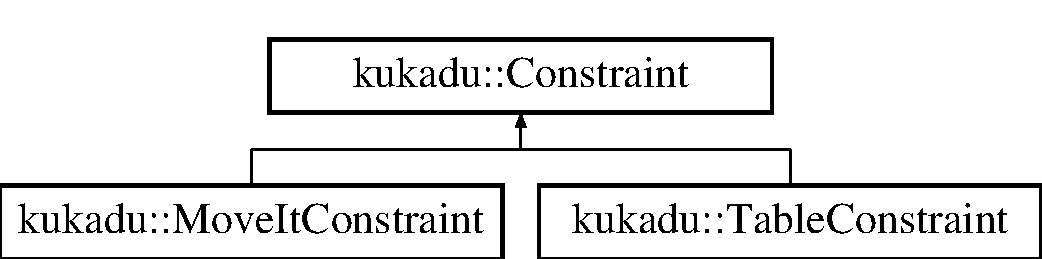
\includegraphics[height=2.000000cm]{classkukadu_1_1Constraint}
\end{center}
\end{figure}
\subsection*{Public Member Functions}
\begin{DoxyCompactItemize}
\item 
\hypertarget{classkukadu_1_1Constraint_aa3991ff85b8e0496b6193da496370eec}{virtual std\-::string {\bfseries get\-Constraint\-Name} ()=0}\label{classkukadu_1_1Constraint_aa3991ff85b8e0496b6193da496370eec}

\item 
\hypertarget{classkukadu_1_1Constraint_a64f1dfe00ed3a4794ef383f9232d7f1c}{virtual bool {\bfseries state\-Ok} (arma\-::vec joint, geometry\-\_\-msgs\-::\-Pose cart\-Pose)=0}\label{classkukadu_1_1Constraint_a64f1dfe00ed3a4794ef383f9232d7f1c}

\end{DoxyCompactItemize}


The documentation for this class was generated from the following file\-:\begin{DoxyCompactItemize}
\item 
/home/c7031109/iis\-\_\-robot\-\_\-sw/iis\-\_\-catkin\-\_\-ws/src/kukadu/include/kukadu/kinematics/constraints/constraints.\-hpp\end{DoxyCompactItemize}

\hypertarget{classkukadu_1_1Controller}{\section{kukadu\-:\-:Controller Class Reference}
\label{classkukadu_1_1Controller}\index{kukadu\-::\-Controller@{kukadu\-::\-Controller}}
}
Inheritance diagram for kukadu\-:\-:Controller\-:\begin{figure}[H]
\begin{center}
\leavevmode
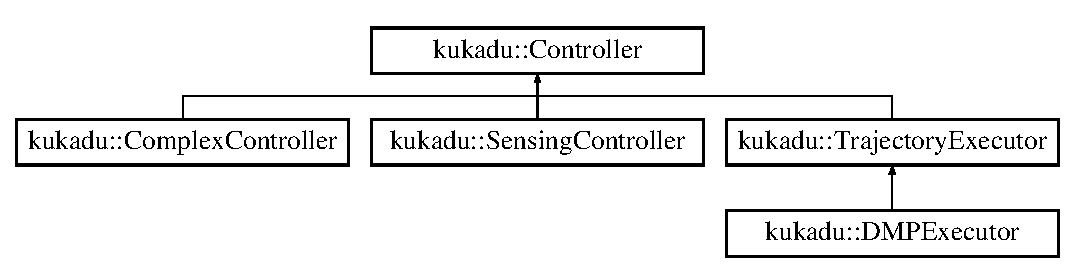
\includegraphics[height=3.000000cm]{classkukadu_1_1Controller}
\end{center}
\end{figure}
\subsection*{Public Member Functions}
\begin{DoxyCompactItemize}
\item 
\hypertarget{classkukadu_1_1Controller_a127838e5505d9d35c68da8d95b9d1cda}{{\bfseries Controller} (std\-::string caption, int simulation\-Failing\-Probability)}\label{classkukadu_1_1Controller_a127838e5505d9d35c68da8d95b9d1cda}

\item 
\hypertarget{classkukadu_1_1Controller_aa27eb73a93a2d59bc0ebe15baf28bea0}{void {\bfseries shut\-Up} ()}\label{classkukadu_1_1Controller_aa27eb73a93a2d59bc0ebe15baf28bea0}

\item 
\hypertarget{classkukadu_1_1Controller_a1973596dea74a0706e275f044ca190b0}{void {\bfseries start\-Talking} ()}\label{classkukadu_1_1Controller_a1973596dea74a0706e275f044ca190b0}

\item 
\hypertarget{classkukadu_1_1Controller_a888ebe1be866cb19e4c8f50eaded5bb9}{virtual void {\bfseries set\-Simulation\-Mode} (bool simulation\-Mode)}\label{classkukadu_1_1Controller_a888ebe1be866cb19e4c8f50eaded5bb9}

\item 
\hypertarget{classkukadu_1_1Controller_aed75e7ede2b67b1803778c6f5f1eb7f7}{virtual bool {\bfseries requires\-Grasp} ()=0}\label{classkukadu_1_1Controller_aed75e7ede2b67b1803778c6f5f1eb7f7}

\item 
\hypertarget{classkukadu_1_1Controller_a181338e971e48966d434c523a7ba5da4}{virtual bool {\bfseries produces\-Grasp} ()=0}\label{classkukadu_1_1Controller_a181338e971e48966d434c523a7ba5da4}

\item 
\hypertarget{classkukadu_1_1Controller_a74a2a16a16104b1bf16ad5eae443e968}{virtual void {\bfseries initialize} ()}\label{classkukadu_1_1Controller_a74a2a16a16104b1bf16ad5eae443e968}

\item 
\hypertarget{classkukadu_1_1Controller_a868b762c6bf33afe14c27dd12806972d}{bool {\bfseries get\-Simulation\-Mode} ()}\label{classkukadu_1_1Controller_a868b762c6bf33afe14c27dd12806972d}

\item 
\hypertarget{classkukadu_1_1Controller_a97ffde82f967a920ddc5efb1c5700b2a}{double {\bfseries get\-Sim\-Failing\-Prob} ()}\label{classkukadu_1_1Controller_a97ffde82f967a920ddc5efb1c5700b2a}

\item 
\hypertarget{classkukadu_1_1Controller_aae1903e89a3af93030bd85cb6baac366}{std\-::string {\bfseries get\-Caption} ()}\label{classkukadu_1_1Controller_aae1903e89a3af93030bd85cb6baac366}

\item 
\hypertarget{classkukadu_1_1Controller_a76ce3ce9867173f014561c0bf28fa69f}{virtual K\-U\-K\-A\-D\-U\-\_\-\-S\-H\-A\-R\-E\-D\-\_\-\-P\-T\-R\\*
$<$ \hyperlink{classkukadu_1_1ControllerResult}{Controller\-Result} $>$ {\bfseries perform\-Action} ()=0}\label{classkukadu_1_1Controller_a76ce3ce9867173f014561c0bf28fa69f}

\end{DoxyCompactItemize}
\subsection*{Protected Member Functions}
\begin{DoxyCompactItemize}
\item 
\hypertarget{classkukadu_1_1Controller_a07c70a71d6028cb711567d55e2010430}{virtual void {\bfseries set\-Simulation\-Mode\-In\-Chain} (bool simulation\-Mode)}\label{classkukadu_1_1Controller_a07c70a71d6028cb711567d55e2010430}

\end{DoxyCompactItemize}
\subsection*{Protected Attributes}
\begin{DoxyCompactItemize}
\item 
\hypertarget{classkukadu_1_1Controller_abeb3dd890d6f8d50306b1b8f9d6b5512}{bool {\bfseries is\-Shut\-Up}}\label{classkukadu_1_1Controller_abeb3dd890d6f8d50306b1b8f9d6b5512}

\end{DoxyCompactItemize}


The documentation for this class was generated from the following files\-:\begin{DoxyCompactItemize}
\item 
/home/c7031109/iis\-\_\-robot\-\_\-sw/iis\-\_\-catkin\-\_\-ws/src/kukadu/include/kukadu/manipulation/controller.\-hpp\item 
/home/c7031109/iis\-\_\-robot\-\_\-sw/iis\-\_\-catkin\-\_\-ws/src/kukadu/src/manipulation/controller.\-cpp\end{DoxyCompactItemize}

\hypertarget{classkukadu_1_1ControllerActionClip}{\section{kukadu\-:\-:Controller\-Action\-Clip Class Reference}
\label{classkukadu_1_1ControllerActionClip}\index{kukadu\-::\-Controller\-Action\-Clip@{kukadu\-::\-Controller\-Action\-Clip}}
}
Inheritance diagram for kukadu\-:\-:Controller\-Action\-Clip\-:\begin{figure}[H]
\begin{center}
\leavevmode
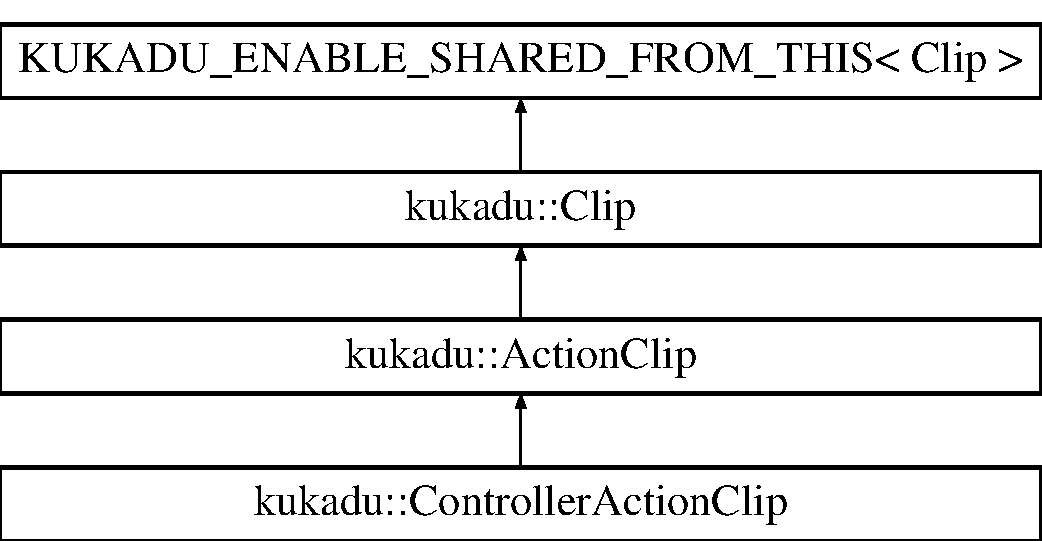
\includegraphics[height=4.000000cm]{classkukadu_1_1ControllerActionClip}
\end{center}
\end{figure}
\subsection*{Public Member Functions}
\begin{DoxyCompactItemize}
\item 
\hypertarget{classkukadu_1_1ControllerActionClip_a45f6b4b5eb168f5ef80da54d4831cbbe}{{\bfseries Controller\-Action\-Clip} (int action\-Id, K\-U\-K\-A\-D\-U\-\_\-\-S\-H\-A\-R\-E\-D\-\_\-\-P\-T\-R$<$ \hyperlink{classkukadu_1_1Controller}{Controller} $>$ action\-Controller, K\-U\-K\-A\-D\-U\-\_\-\-S\-H\-A\-R\-E\-D\-\_\-\-P\-T\-R$<$ kukadu\-\_\-mersenne\-\_\-twister $>$ generator)}\label{classkukadu_1_1ControllerActionClip_a45f6b4b5eb168f5ef80da54d4831cbbe}

\item 
\hypertarget{classkukadu_1_1ControllerActionClip_acd8f9275a19a8d30d127a61e54593060}{void {\bfseries perform\-Action} ()}\label{classkukadu_1_1ControllerActionClip_acd8f9275a19a8d30d127a61e54593060}

\item 
\hypertarget{classkukadu_1_1ControllerActionClip_a6c2d2f8dde18dd4294eaab5060ce62bf}{virtual std\-::string {\bfseries to\-String} () const }\label{classkukadu_1_1ControllerActionClip_a6c2d2f8dde18dd4294eaab5060ce62bf}

\item 
\hypertarget{classkukadu_1_1ControllerActionClip_a2154f9c71a3c74fb7ab78d8fd7f40e22}{K\-U\-K\-A\-D\-U\-\_\-\-S\-H\-A\-R\-E\-D\-\_\-\-P\-T\-R$<$ \hyperlink{classkukadu_1_1Controller}{Controller} $>$ {\bfseries get\-Action\-Controller} ()}\label{classkukadu_1_1ControllerActionClip_a2154f9c71a3c74fb7ab78d8fd7f40e22}

\end{DoxyCompactItemize}
\subsection*{Additional Inherited Members}


The documentation for this class was generated from the following files\-:\begin{DoxyCompactItemize}
\item 
/home/c7031109/iis\-\_\-robot\-\_\-sw/iis\-\_\-catkin\-\_\-ws/src/kukadu/include/kukadu/manipulation/haptic/controlleractionclip.\-hpp\item 
/home/c7031109/iis\-\_\-robot\-\_\-sw/iis\-\_\-catkin\-\_\-ws/src/kukadu/src/manipulation/haptic/controlleractionclip.\-cpp\end{DoxyCompactItemize}

\hypertarget{classkukadu_1_1ControllerResult}{\section{kukadu\-:\-:Controller\-Result Class Reference}
\label{classkukadu_1_1ControllerResult}\index{kukadu\-::\-Controller\-Result@{kukadu\-::\-Controller\-Result}}
}
Inheritance diagram for kukadu\-:\-:Controller\-Result\-:\begin{figure}[H]
\begin{center}
\leavevmode
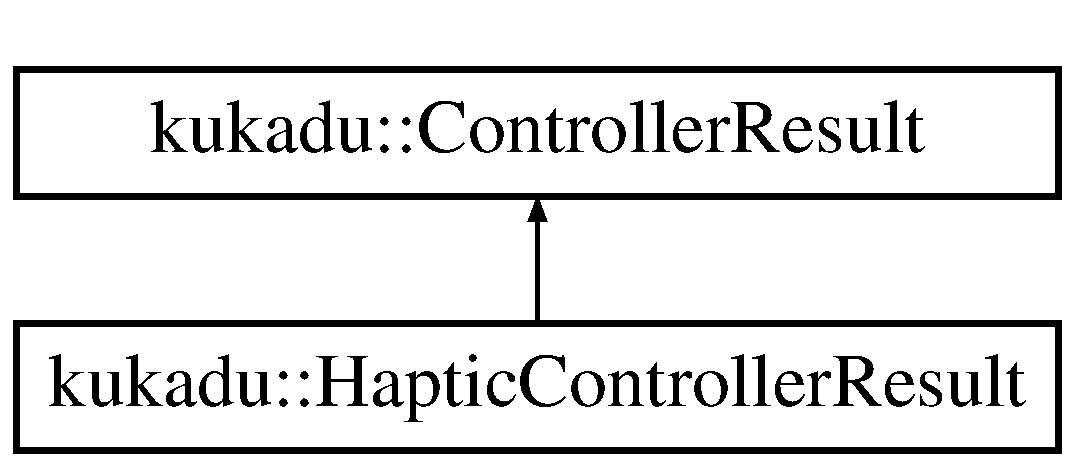
\includegraphics[height=2.000000cm]{classkukadu_1_1ControllerResult}
\end{center}
\end{figure}
\subsection*{Public Member Functions}
\begin{DoxyCompactItemize}
\item 
\hypertarget{classkukadu_1_1ControllerResult_ad2ed8a808d635b2b6f3183ae9447bd0c}{{\bfseries Controller\-Result} (arma\-::vec t, std\-::vector$<$ arma\-::vec $>$ ys, bool success)}\label{classkukadu_1_1ControllerResult_ad2ed8a808d635b2b6f3183ae9447bd0c}

\item 
\hypertarget{classkukadu_1_1ControllerResult_a26edcc9c10dccd4c53c18e081712ed48}{arma\-::vec {\bfseries get\-Times} ()}\label{classkukadu_1_1ControllerResult_a26edcc9c10dccd4c53c18e081712ed48}

\item 
\hypertarget{classkukadu_1_1ControllerResult_a6d39870fa7743699c4376562f687a56b}{std\-::vector$<$ arma\-::vec $>$ {\bfseries get\-Ys} ()}\label{classkukadu_1_1ControllerResult_a6d39870fa7743699c4376562f687a56b}

\item 
\hypertarget{classkukadu_1_1ControllerResult_a77c5a596b26000f06ee1138ce62c82a7}{void {\bfseries set\-Success} (bool success)}\label{classkukadu_1_1ControllerResult_a77c5a596b26000f06ee1138ce62c82a7}

\item 
\hypertarget{classkukadu_1_1ControllerResult_aeb935f4206986fea6d5762e4c31298b6}{bool {\bfseries get\-Success} ()}\label{classkukadu_1_1ControllerResult_aeb935f4206986fea6d5762e4c31298b6}

\end{DoxyCompactItemize}


The documentation for this class was generated from the following files\-:\begin{DoxyCompactItemize}
\item 
/home/c7031109/iis\-\_\-robot\-\_\-sw/iis\-\_\-catkin\-\_\-ws/src/kukadu/include/kukadu/types/controllerresult.\-hpp\item 
/home/c7031109/iis\-\_\-robot\-\_\-sw/iis\-\_\-catkin\-\_\-ws/src/kukadu/src/types/controllerresult.\-cpp\end{DoxyCompactItemize}

\hypertarget{classkukadu_1_1ControlQueue}{\section{kukadu\-:\-:Control\-Queue Class Reference}
\label{classkukadu_1_1ControlQueue}\index{kukadu\-::\-Control\-Queue@{kukadu\-::\-Control\-Queue}}
}


Interface between the kukadu software stack and the robot hardware. If kukadu shall support another robot, the abstract methods need to be implemented according to the documentation. Then the kukadu software stack is available for usage with the robot.  




{\ttfamily \#include $<$controlqueue.\-hpp$>$}

Inheritance diagram for kukadu\-:\-:Control\-Queue\-:\begin{figure}[H]
\begin{center}
\leavevmode
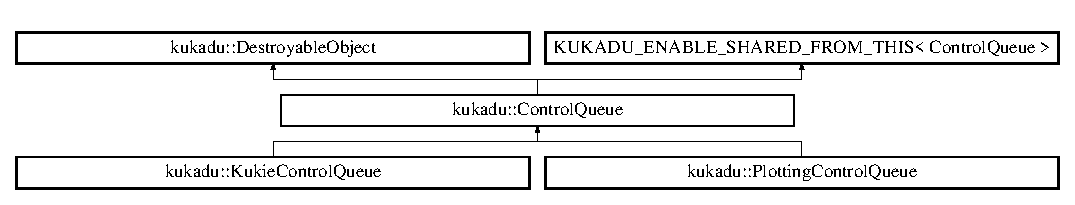
\includegraphics[height=2.301370cm]{classkukadu_1_1ControlQueue}
\end{center}
\end{figure}
\subsection*{Public Member Functions}
\begin{DoxyCompactItemize}
\item 
\hyperlink{classkukadu_1_1ControlQueue_a946b967c77d0b6d663239fa60ff602f9}{Control\-Queue} (int deg\-Of\-Freedom, double desired\-Cycle\-Time)
\begin{DoxyCompactList}\small\item\em Constructor taking the robot dependent degrees of freedom. \end{DoxyCompactList}\item 
int \hyperlink{classkukadu_1_1ControlQueue_aaa583d0b0c04c7f0acc869cca0e8ef41}{get\-Movement\-Degrees\-Of\-Freedom} ()
\begin{DoxyCompactList}\small\item\em Returns number of the robots degrees of freedom. \end{DoxyCompactList}\item 
void \hyperlink{classkukadu_1_1ControlQueue_a5245ff31c7dea26070743d1f6560801c}{set\-Cycle\-Time} (double cycle\-Time)
\begin{DoxyCompactList}\small\item\em Sets the queue cycle time. \end{DoxyCompactList}\item 
\hypertarget{classkukadu_1_1ControlQueue_a35d6a6e4e7c8467691c11567fe21f340}{K\-U\-K\-A\-D\-U\-\_\-\-S\-H\-A\-R\-E\-D\-\_\-\-P\-T\-R$<$ kukadu\-\_\-thread $>$ \hyperlink{classkukadu_1_1ControlQueue_a35d6a6e4e7c8467691c11567fe21f340}{start\-Queue} ()}\label{classkukadu_1_1ControlQueue_a35d6a6e4e7c8467691c11567fe21f340}

\begin{DoxyCompactList}\small\item\em Starts new thread to control the robot with real time capability. \end{DoxyCompactList}\item 
virtual double \hyperlink{classkukadu_1_1ControlQueue_a82349f67c4ea6f2dc2689e765717d8e2}{get\-Cycle\-Time} ()
\begin{DoxyCompactList}\small\item\em Returns the time between two cycles. \end{DoxyCompactList}\item 
virtual bool \hyperlink{classkukadu_1_1ControlQueue_aa02fcb2c8cd2c1c8ca553ae636000beb}{get\-Queue\-Running} ()
\begin{DoxyCompactList}\small\item\em Returns whether or not the queue is currently running. \end{DoxyCompactList}\item 
\hypertarget{classkukadu_1_1ControlQueue_a8d413404960c7597032876396777e38f}{virtual void \hyperlink{classkukadu_1_1ControlQueue_a8d413404960c7597032876396777e38f}{stop\-Queue} ()}\label{classkukadu_1_1ControlQueue_a8d413404960c7597032876396777e38f}

\begin{DoxyCompactList}\small\item\em Stops the queue. \end{DoxyCompactList}\item 
\hypertarget{classkukadu_1_1ControlQueue_a0025c5c010a1b33d637e52fb24f767b2}{virtual void \hyperlink{classkukadu_1_1ControlQueue_a0025c5c010a1b33d637e52fb24f767b2}{set\-Next\-Trajectory} (std\-::vector$<$ arma\-::vec $>$ joint\-Trajectory)}\label{classkukadu_1_1ControlQueue_a0025c5c010a1b33d637e52fb24f767b2}

\begin{DoxyCompactList}\small\item\em With \hyperlink{classkukadu_1_1ControlQueue_a0025c5c010a1b33d637e52fb24f767b2}{set\-Next\-Trajectory()} a complete trajectory can be added to the queue. The trajectory will be executed after all other added commands (already contained in the queue) were executed. \end{DoxyCompactList}\item 
virtual void \hyperlink{classkukadu_1_1ControlQueue_aca70a978b2950d7c9ab99d55c5977eec}{move} (arma\-::vec joints)
\begin{DoxyCompactList}\small\item\em Adds next joint position to the end of the queue (can be used for trajectory following) \end{DoxyCompactList}\item 
virtual void \hyperlink{classkukadu_1_1ControlQueue_a62b3e0c02b1937b09ae538a71ee0e855}{move} (geometry\-\_\-msgs\-::\-Pose pose)
\begin{DoxyCompactList}\small\item\em Adds next cartesian position to the end of the queue (can be used for trajectory following) \end{DoxyCompactList}\item 
virtual void \hyperlink{classkukadu_1_1ControlQueue_a5defe63d9f1b9829676f9a31a4683911}{switch\-Mode} (int mode)
\begin{DoxyCompactList}\small\item\em Switches robot modes. A state might be a real time command mode or monitoring mode. \end{DoxyCompactList}\item 
\hypertarget{classkukadu_1_1ControlQueue_ae4236dc4c31aff57d2295dd11dbf453b}{virtual void \hyperlink{classkukadu_1_1ControlQueue_ae4236dc4c31aff57d2295dd11dbf453b}{stop\-Current\-Mode} ()}\label{classkukadu_1_1ControlQueue_ae4236dc4c31aff57d2295dd11dbf453b}

\begin{DoxyCompactList}\small\item\em Stops current mode and switches back to default mode (e.\-g. monitoring mode) \end{DoxyCompactList}\item 
virtual void \hyperlink{classkukadu_1_1ControlQueue_a324484e79a5505656a32d9f32054e5d0}{synchronize\-To\-Queue} (int max\-Num\-Joints\-In\-Queue)
\begin{DoxyCompactList}\small\item\em Blocks, if more than the defined maximum element count is in the queue. \end{DoxyCompactList}\item 
virtual void \hyperlink{classkukadu_1_1ControlQueue_a225130ca0fa4a22e98cc0e5679917841}{set\-Starting\-Joints} (arma\-::vec joints)
\begin{DoxyCompactList}\small\item\em If this is set, the robot moves to the desired position by \hyperlink{classkukadu_1_1ControlQueue_ad11059100321b24a1af8ef7de8314353}{joint\-Ptp()} before the queue is started. \end{DoxyCompactList}\item 
virtual std\-::vector$<$ \hyperlink{structmes__result}{mes\-\_\-result} $>$ \hyperlink{classkukadu_1_1ControlQueue_ad11059100321b24a1af8ef7de8314353}{joint\-Ptp} (arma\-::vec joints)
\begin{DoxyCompactList}\small\item\em Implements simple point to point movement in joint space (blocks until target reached) \end{DoxyCompactList}\item 
K\-U\-K\-A\-D\-U\-\_\-\-S\-H\-A\-R\-E\-D\-\_\-\-P\-T\-R$<$ kukadu\-\_\-thread $>$ \hyperlink{classkukadu_1_1ControlQueue_aaf35ae626b08ac53508acdc84ab58c8f}{joint\-Ptp\-Nb} (arma\-::vec joints)
\begin{DoxyCompactList}\small\item\em Implements simple point to point movement in joint space (not blocking) \end{DoxyCompactList}\item 
virtual std\-::vector$<$ \hyperlink{structmes__result}{mes\-\_\-result} $>$ \hyperlink{classkukadu_1_1ControlQueue_a1bfa23a8ce6319f6ef0ed9208e896054}{cartesian\-Ptp} (geometry\-\_\-msgs\-::\-Pose pos)
\begin{DoxyCompactList}\small\item\em Implements simple point to point movement in cartesian space. \end{DoxyCompactList}\item 
virtual std\-::vector$<$ \hyperlink{structmes__result}{mes\-\_\-result} $>$ \hyperlink{classkukadu_1_1ControlQueue_a58518838c503e7eaa9c220bdf34ddd33}{cartesian\-Ptp} (geometry\-\_\-msgs\-::\-Pose pos, double max\-Force)
\begin{DoxyCompactList}\small\item\em Implements simple point to point movement in cartesian space. \end{DoxyCompactList}\item 
virtual K\-U\-K\-A\-D\-U\-\_\-\-S\-H\-A\-R\-E\-D\-\_\-\-P\-T\-R\\*
$<$ kukadu\-\_\-thread $>$ \hyperlink{classkukadu_1_1ControlQueue_a1c0ad5ad4d3af98f26d0c633181df010}{cartesian\-Ptp\-Nb} (geometry\-\_\-msgs\-::\-Pose pos)
\begin{DoxyCompactList}\small\item\em Implements simple point to point movement in cartesian space (does not block until the position is reached) \end{DoxyCompactList}\item 
virtual void \hyperlink{classkukadu_1_1ControlQueue_a18e628686b8c86abfdbd097b60aa5768}{set\-Additional\-Load} (float load\-Mass, float load\-Pos)=0
\begin{DoxyCompactList}\small\item\em Changes the expected load data of the robot (e.\-g. can be used whenever robot picks up an object). Some robots might require this information in order to avoid control problems. \end{DoxyCompactList}\item 
virtual void \hyperlink{classkukadu_1_1ControlQueue_aee25e6410909af34d740edbece98d677}{set\-Stiffness} (float cpstiffnessxyz, float cpstiffnessabc, float cpdamping, float cpmaxdelta, float maxforce, float axismaxdeltatrq)=0
\begin{DoxyCompactList}\small\item\em Sets certain stiffness parameters in cartesian space (if the robot supports this) according to a mass spring damper system model. \end{DoxyCompactList}\item 
virtual \hyperlink{structmes__result}{mes\-\_\-result} \hyperlink{classkukadu_1_1ControlQueue_abddacca2f9bf2db7a42a80d347843cec}{get\-Current\-Cartesian\-Pos} ()
\begin{DoxyCompactList}\small\item\em Returns the current robot position in cartesian space. \end{DoxyCompactList}\item 
virtual geometry\-\_\-msgs\-::\-Pose \hyperlink{classkukadu_1_1ControlQueue_a9e79e1d0d9697bbf146d66a2d01fea9e}{get\-Current\-Cartesian\-Pose} ()=0
\begin{DoxyCompactList}\small\item\em Returns current robot position in cartesian space. \end{DoxyCompactList}\item 
virtual arma\-::vec \hyperlink{classkukadu_1_1ControlQueue_a53b2ecff4ae71b1e01d18793f63645ce}{get\-Starting\-Joints} ()
\begin{DoxyCompactList}\small\item\em Returns the robot joints the robot has been directly before starting command mode. \end{DoxyCompactList}\item 
virtual \hyperlink{structmes__result}{mes\-\_\-result} \hyperlink{classkukadu_1_1ControlQueue_a6ba7b6db5099073eadd7bc04792bc643}{get\-Current\-Joints} ()=0
\begin{DoxyCompactList}\small\item\em Returns joints if the robot is in command mode. \end{DoxyCompactList}\item 
virtual \hyperlink{structmes__result}{mes\-\_\-result} \hyperlink{classkukadu_1_1ControlQueue_a1468c1771ea7dfd1ee3b0a7279407241}{get\-Current\-Jnt\-Frc} ()=0
\begin{DoxyCompactList}\small\item\em Returns the forces measured for the robot joints. \end{DoxyCompactList}\item 
virtual \hyperlink{structmes__result}{mes\-\_\-result} \hyperlink{classkukadu_1_1ControlQueue_aa557f386f03cfb4986ed7cd9997212ab}{get\-Current\-Cartesian\-Frc\-Trq} ()=0
\begin{DoxyCompactList}\small\item\em Returns the forces and torques measured at the robot end-\/effector. \end{DoxyCompactList}\item 
virtual void \hyperlink{classkukadu_1_1ControlQueue_a5af587fff906cf978225a317e701d41f}{set\-Jnt\-Ptp\-Thresh} (double thresh)=0
\begin{DoxyCompactList}\small\item\em Sets the maximum deviation in joint space that is tolerated for a point to point movement. \end{DoxyCompactList}\item 
virtual bool \hyperlink{classkukadu_1_1ControlQueue_ac6e06776a9e03107aabc111ef5ce2b6d}{is\-Initialized} ()
\begin{DoxyCompactList}\small\item\em Returns true if the command mode initialization is done. \end{DoxyCompactList}\item 
virtual std\-::string \hyperlink{classkukadu_1_1ControlQueue_aff34133be55d32e07d0ce6aac26cf10d}{get\-Robot\-Name} ()=0
\begin{DoxyCompactList}\small\item\em Returns the robot name. \end{DoxyCompactList}\item 
virtual std\-::string \hyperlink{classkukadu_1_1ControlQueue_aab7dbf0d07b829b9612cfe7141c801a1}{get\-Robot\-File\-Name} ()=0
\begin{DoxyCompactList}\small\item\em Returns the robot name with escaped special characaters (e.\-g. white spaces) \end{DoxyCompactList}\item 
virtual std\-::vector$<$ std\-::string $>$ \hyperlink{classkukadu_1_1ControlQueue_a85702573cb64f7f3dd9c3d2eac95a6ea}{get\-Joint\-Names} ()=0
\begin{DoxyCompactList}\small\item\em Returns the robot joint names. \end{DoxyCompactList}\item 
virtual double \hyperlink{classkukadu_1_1ControlQueue_a550f23320f1b124b1cd587605317e37c}{get\-Absolute\-Cart\-Force} ()
\begin{DoxyCompactList}\small\item\em Returns currently measured absolute force on the end-\/effector. \end{DoxyCompactList}\item 
\hypertarget{classkukadu_1_1ControlQueue_a8e76e19772053274046193436b0cae1c}{virtual void \hyperlink{classkukadu_1_1ControlQueue_a8e76e19772053274046193436b0cae1c}{shut\-Up} ()}\label{classkukadu_1_1ControlQueue_a8e76e19772053274046193436b0cae1c}

\begin{DoxyCompactList}\small\item\em Prevents the queue from printing debug information to the terminal. \end{DoxyCompactList}\item 
\hypertarget{classkukadu_1_1ControlQueue_ac9042952868522099628074d22d61742}{virtual void \hyperlink{classkukadu_1_1ControlQueue_ac9042952868522099628074d22d61742}{start\-Talking} ()}\label{classkukadu_1_1ControlQueue_ac9042952868522099628074d22d61742}

\begin{DoxyCompactList}\small\item\em Makes the queue printing debug information to the terminal. \end{DoxyCompactList}\item 
virtual void \hyperlink{classkukadu_1_1ControlQueue_a650c486b9f78d3dec1db8741b575a0ab}{roll\-Back} (double time)
\begin{DoxyCompactList}\small\item\em If the rollback mode is started by \hyperlink{classkukadu_1_1ControlQueue_acb6ba5c61e9c26dcaa8e4073946e3791}{start\-Roll\-Back\-Mode()} the robot can stop the current execution and move backwards the same trajectory it came. Therefore it can move back in time for a given time (in seconds) \end{DoxyCompactList}\item 
\hypertarget{classkukadu_1_1ControlQueue_a38ba0b9fffb0fff6d39d742b1a2eb76b}{virtual void \hyperlink{classkukadu_1_1ControlQueue_a38ba0b9fffb0fff6d39d742b1a2eb76b}{stop\-Joint\-Roll\-Back\-Mode} ()}\label{classkukadu_1_1ControlQueue_a38ba0b9fffb0fff6d39d742b1a2eb76b}

\begin{DoxyCompactList}\small\item\em Stops the rollback mode (see \hyperlink{classkukadu_1_1ControlQueue_acb6ba5c61e9c26dcaa8e4073946e3791}{start\-Roll\-Back\-Mode()}) \end{DoxyCompactList}\item 
virtual void \hyperlink{classkukadu_1_1ControlQueue_acb6ba5c61e9c26dcaa8e4073946e3791}{start\-Roll\-Back\-Mode} (double possible\-Time\-Reach)
\begin{DoxyCompactList}\small\item\em Starts the rollback mode. When the function \hyperlink{classkukadu_1_1ControlQueue_a650c486b9f78d3dec1db8741b575a0ab}{roll\-Back()} is called the robot can roll back the current trajectory for at most a the given time (in seconds). This mode is only available in joint space execution. \end{DoxyCompactList}\item 
virtual double \hyperlink{classkukadu_1_1ControlQueue_a35a0fc7a7b46b1f77dc6c4c8e34e5e58}{get\-Current\-Time} ()
\begin{DoxyCompactList}\small\item\em An intrinsic clock is started with \hyperlink{classkukadu_1_1ControlQueue_a35d6a6e4e7c8467691c11567fe21f340}{start\-Queue()}. This method returns the current time according to this clock. \end{DoxyCompactList}\item 
bool \hyperlink{classkukadu_1_1ControlQueue_af8d1c646ba20dc854675b6af5fcb6701}{is\-Shut\-Up} ()
\begin{DoxyCompactList}\small\item\em Indicates whether or not the queue is printing debug information to the terminal (see \hyperlink{classkukadu_1_1ControlQueue_a8e76e19772053274046193436b0cae1c}{shut\-Up()}). \end{DoxyCompactList}\item 
virtual int \hyperlink{classkukadu_1_1ControlQueue_afce92074c674d8a1b0127190fd0603cf}{get\-Current\-Mode} ()=0
\begin{DoxyCompactList}\small\item\em Returns the current robot control mode (see \hyperlink{classkukadu_1_1ControlQueue_a5defe63d9f1b9829676f9a31a4683911}{switch\-Mode()}) \end{DoxyCompactList}\end{DoxyCompactItemize}
\subsection*{Static Public Attributes}
\begin{DoxyCompactItemize}
\item 
\hypertarget{classkukadu_1_1ControlQueue_a1a207e4332a8b1ac5a8bf425d697570f}{static const int {\bfseries C\-O\-N\-T\-R\-O\-L\-Q\-U\-E\-U\-E\-\_\-\-S\-T\-O\-P\-\_\-\-M\-O\-D\-E} = 0}\label{classkukadu_1_1ControlQueue_a1a207e4332a8b1ac5a8bf425d697570f}

\item 
\hypertarget{classkukadu_1_1ControlQueue_a9c8511060b437868de842e7456f18018}{static const int {\bfseries C\-O\-N\-T\-R\-O\-L\-Q\-U\-E\-U\-E\-\_\-\-J\-N\-T\-\_\-\-P\-O\-S\-\_\-\-M\-O\-D\-E} = 10}\label{classkukadu_1_1ControlQueue_a9c8511060b437868de842e7456f18018}

\item 
\hypertarget{classkukadu_1_1ControlQueue_a664a52e365e9185a0aef587e331fe94f}{static const int {\bfseries C\-O\-N\-T\-R\-O\-L\-Q\-U\-E\-U\-E\-\_\-\-C\-A\-R\-T\-\_\-\-I\-M\-P\-\_\-\-M\-O\-D\-E} = 20}\label{classkukadu_1_1ControlQueue_a664a52e365e9185a0aef587e331fe94f}

\item 
\hypertarget{classkukadu_1_1ControlQueue_a8372490df9e7fbfa75afb9cfe1c0e6b4}{static const int {\bfseries C\-O\-N\-T\-R\-O\-L\-Q\-U\-E\-U\-E\-\_\-\-J\-N\-T\-\_\-\-I\-M\-P\-\_\-\-M\-O\-D\-E} = 30}\label{classkukadu_1_1ControlQueue_a8372490df9e7fbfa75afb9cfe1c0e6b4}

\end{DoxyCompactItemize}
\subsection*{Protected Member Functions}
\begin{DoxyCompactItemize}
\item 
\hypertarget{classkukadu_1_1ControlQueue_ac38a2bac4927cf5d424e735af703f199}{virtual void \hyperlink{classkukadu_1_1ControlQueue_ac38a2bac4927cf5d424e735af703f199}{set\-Deg\-Of\-Freedom} (int deg\-Of\-Freedom)}\label{classkukadu_1_1ControlQueue_ac38a2bac4927cf5d424e735af703f199}

\begin{DoxyCompactList}\small\item\em Can be used to set the number of degrees of freedom. \end{DoxyCompactList}\item 
\hypertarget{classkukadu_1_1ControlQueue_a743fbc08007b777393a6f14d66ed2e8a}{virtual void \hyperlink{classkukadu_1_1ControlQueue_a743fbc08007b777393a6f14d66ed2e8a}{set\-Init\-Values} ()=0}\label{classkukadu_1_1ControlQueue_a743fbc08007b777393a6f14d66ed2e8a}

\begin{DoxyCompactList}\small\item\em This method can be used to initialize custom parts of the \hyperlink{classkukadu_1_1ControlQueue}{Control\-Queue} implementation before the queue is started by \hyperlink{classkukadu_1_1ControlQueue_a35d6a6e4e7c8467691c11567fe21f340}{start\-Queue()}. \end{DoxyCompactList}\item 
\hypertarget{classkukadu_1_1ControlQueue_a89a7b21307ccd0759a9e8b8e483cb919}{virtual void \hyperlink{classkukadu_1_1ControlQueue_a89a7b21307ccd0759a9e8b8e483cb919}{joint\-Ptp\-Internal} (arma\-::vec joints)=0}\label{classkukadu_1_1ControlQueue_a89a7b21307ccd0759a9e8b8e483cb919}

\begin{DoxyCompactList}\small\item\em The control queue collects the data about the actually executed trajectory during a point to point movement. This is automatically done by \hyperlink{classkukadu_1_1ControlQueue_ad11059100321b24a1af8ef7de8314353}{joint\-Ptp()}. \hyperlink{classkukadu_1_1ControlQueue_ad11059100321b24a1af8ef7de8314353}{joint\-Ptp()} calls the \hyperlink{classkukadu_1_1ControlQueue_a89a7b21307ccd0759a9e8b8e483cb919}{joint\-Ptp\-Internal()} function that actually plans the movement in joint space and executes it. \end{DoxyCompactList}\item 
\hypertarget{classkukadu_1_1ControlQueue_a12166afa17d758aa6b43362fc999e146}{virtual void \hyperlink{classkukadu_1_1ControlQueue_a12166afa17d758aa6b43362fc999e146}{submit\-Next\-Joint\-Move} (arma\-::vec joints)=0}\label{classkukadu_1_1ControlQueue_a12166afa17d758aa6b43362fc999e146}

\begin{DoxyCompactList}\small\item\em This method is called by the run() method once per clock cycle and actually submits the command about the next desired joint pose to the robot. \end{DoxyCompactList}\item 
\hypertarget{classkukadu_1_1ControlQueue_a910db788a6da11006d358a84197bff23}{virtual void \hyperlink{classkukadu_1_1ControlQueue_a910db788a6da11006d358a84197bff23}{submit\-Next\-Cart\-Move} (geometry\-\_\-msgs\-::\-Pose pose)=0}\label{classkukadu_1_1ControlQueue_a910db788a6da11006d358a84197bff23}

\begin{DoxyCompactList}\small\item\em This method is called by the run() method once per clock cycle and actually submits the command about the next desired Cartesian pose to the robot. \end{DoxyCompactList}\item 
\hypertarget{classkukadu_1_1ControlQueue_a76e7bf30b8e694c0db9bec92e06529a0}{virtual void \hyperlink{classkukadu_1_1ControlQueue_a76e7bf30b8e694c0db9bec92e06529a0}{set\-Current\-Control\-Type\-Internal} (int control\-Type)=0}\label{classkukadu_1_1ControlQueue_a76e7bf30b8e694c0db9bec92e06529a0}

\begin{DoxyCompactList}\small\item\em This method is called by \hyperlink{classkukadu_1_1ControlQueue_a5defe63d9f1b9829676f9a31a4683911}{switch\-Mode()} and actually sends the control mode command to the robot. \end{DoxyCompactList}\item 
\hypertarget{classkukadu_1_1ControlQueue_a13059c37abe4846a356e0cfcf10958b9}{virtual void \hyperlink{classkukadu_1_1ControlQueue_a13059c37abe4846a356e0cfcf10958b9}{cart\-Ptp\-Internal} (geometry\-\_\-msgs\-::\-Pose pose, double max\-Force)=0}\label{classkukadu_1_1ControlQueue_a13059c37abe4846a356e0cfcf10958b9}

\begin{DoxyCompactList}\small\item\em The control queue collects the data about the actually executed trajectory during a point to point movement. This is automatically done by \hyperlink{classkukadu_1_1ControlQueue_a1bfa23a8ce6319f6ef0ed9208e896054}{cartesian\-Ptp()}. \hyperlink{classkukadu_1_1ControlQueue_a1bfa23a8ce6319f6ef0ed9208e896054}{cartesian\-Ptp()} calls the \hyperlink{classkukadu_1_1ControlQueue_a13059c37abe4846a356e0cfcf10958b9}{cart\-Ptp\-Internal()} function that actually plans the movement in Cartesian space and executes it. \end{DoxyCompactList}\item 
\hypertarget{classkukadu_1_1ControlQueue_a87d7c2d918d0ca720eeae609959d4d78}{virtual void \hyperlink{classkukadu_1_1ControlQueue_a87d7c2d918d0ca720eeae609959d4d78}{start\-Queue\-Hook} ()=0}\label{classkukadu_1_1ControlQueue_a87d7c2d918d0ca720eeae609959d4d78}

\begin{DoxyCompactList}\small\item\em This method can be used to add some additional initialization behavior when the queue is started. If no additional initialization is required, the method can be left empty. \end{DoxyCompactList}\item 
virtual bool \hyperlink{classkukadu_1_1ControlQueue_a6ebb66d1bd2188e1fca3ee1440b8c0fe}{stop\-Queue\-While\-Ptp} ()=0
\begin{DoxyCompactList}\small\item\em This method determines, if the queue execetion should be stopped while ptp commands are executed (this is typically the case when ptp is done outside of the control queue implementation). If two different controls interfere it can result in dangerous behaviour. \end{DoxyCompactList}\end{DoxyCompactItemize}
\subsection*{Protected Attributes}
\begin{DoxyCompactItemize}
\item 
\hypertarget{classkukadu_1_1ControlQueue_aadba228efd6e34095ce7d52bc94a4d29}{int {\bfseries current\-Control\-Type}}\label{classkukadu_1_1ControlQueue_aadba228efd6e34095ce7d52bc94a4d29}

\end{DoxyCompactItemize}


\subsection{Detailed Description}
Interface between the kukadu software stack and the robot hardware. If kukadu shall support another robot, the abstract methods need to be implemented according to the documentation. Then the kukadu software stack is available for usage with the robot. 

The \hyperlink{classkukadu_1_1ControlQueue}{Control\-Queue} interface is the bridge between all implemented control methods (D\-M\-Ps, ...) and the robot hardware. It supports functionlity such as trajectory following, simple point to point planning or security mechanisms such as maximum force values for execution. 

\subsection{Constructor \& Destructor Documentation}
\hypertarget{classkukadu_1_1ControlQueue_a946b967c77d0b6d663239fa60ff602f9}{\index{kukadu\-::\-Control\-Queue@{kukadu\-::\-Control\-Queue}!Control\-Queue@{Control\-Queue}}
\index{Control\-Queue@{Control\-Queue}!kukadu::ControlQueue@{kukadu\-::\-Control\-Queue}}
\subsubsection[{Control\-Queue}]{\setlength{\rightskip}{0pt plus 5cm}kukadu\-::\-Control\-Queue\-::\-Control\-Queue (
\begin{DoxyParamCaption}
\item[{int}]{deg\-Of\-Freedom, }
\item[{double}]{desired\-Cycle\-Time}
\end{DoxyParamCaption}
)}}\label{classkukadu_1_1ControlQueue_a946b967c77d0b6d663239fa60ff602f9}


Constructor taking the robot dependent degrees of freedom. 


\begin{DoxyParams}{Parameters}
{\em deg\-Of\-Freedom} & number of robots degrees of freedom \\
\hline
\end{DoxyParams}


\subsection{Member Function Documentation}
\hypertarget{classkukadu_1_1ControlQueue_a1bfa23a8ce6319f6ef0ed9208e896054}{\index{kukadu\-::\-Control\-Queue@{kukadu\-::\-Control\-Queue}!cartesian\-Ptp@{cartesian\-Ptp}}
\index{cartesian\-Ptp@{cartesian\-Ptp}!kukadu::ControlQueue@{kukadu\-::\-Control\-Queue}}
\subsubsection[{cartesian\-Ptp}]{\setlength{\rightskip}{0pt plus 5cm}std\-::vector$<$ {\bf mes\-\_\-result} $>$ kukadu\-::\-Control\-Queue\-::cartesian\-Ptp (
\begin{DoxyParamCaption}
\item[{geometry\-\_\-msgs\-::\-Pose}]{pos}
\end{DoxyParamCaption}
)\hspace{0.3cm}{\ttfamily [virtual]}}}\label{classkukadu_1_1ControlQueue_a1bfa23a8ce6319f6ef0ed9208e896054}


Implements simple point to point movement in cartesian space. 


\begin{DoxyParams}{Parameters}
{\em pose} & of end-\/effector \\
\hline
\end{DoxyParams}
\hypertarget{classkukadu_1_1ControlQueue_a58518838c503e7eaa9c220bdf34ddd33}{\index{kukadu\-::\-Control\-Queue@{kukadu\-::\-Control\-Queue}!cartesian\-Ptp@{cartesian\-Ptp}}
\index{cartesian\-Ptp@{cartesian\-Ptp}!kukadu::ControlQueue@{kukadu\-::\-Control\-Queue}}
\subsubsection[{cartesian\-Ptp}]{\setlength{\rightskip}{0pt plus 5cm}std\-::vector$<$ {\bf mes\-\_\-result} $>$ kukadu\-::\-Control\-Queue\-::cartesian\-Ptp (
\begin{DoxyParamCaption}
\item[{geometry\-\_\-msgs\-::\-Pose}]{pos, }
\item[{double}]{max\-Force}
\end{DoxyParamCaption}
)\hspace{0.3cm}{\ttfamily [virtual]}}}\label{classkukadu_1_1ControlQueue_a58518838c503e7eaa9c220bdf34ddd33}


Implements simple point to point movement in cartesian space. 


\begin{DoxyParams}{Parameters}
{\em pose} & of end-\/effector \\
\hline
{\em max\-Force} & the point to point movement is stopped if the observed force exceeds this value (in Newton) \\
\hline
\end{DoxyParams}
\hypertarget{classkukadu_1_1ControlQueue_a1c0ad5ad4d3af98f26d0c633181df010}{\index{kukadu\-::\-Control\-Queue@{kukadu\-::\-Control\-Queue}!cartesian\-Ptp\-Nb@{cartesian\-Ptp\-Nb}}
\index{cartesian\-Ptp\-Nb@{cartesian\-Ptp\-Nb}!kukadu::ControlQueue@{kukadu\-::\-Control\-Queue}}
\subsubsection[{cartesian\-Ptp\-Nb}]{\setlength{\rightskip}{0pt plus 5cm}K\-U\-K\-A\-D\-U\-\_\-\-S\-H\-A\-R\-E\-D\-\_\-\-P\-T\-R$<$ kukadu\-\_\-thread $>$ kukadu\-::\-Control\-Queue\-::cartesian\-Ptp\-Nb (
\begin{DoxyParamCaption}
\item[{geometry\-\_\-msgs\-::\-Pose}]{pos}
\end{DoxyParamCaption}
)\hspace{0.3cm}{\ttfamily [virtual]}}}\label{classkukadu_1_1ControlQueue_a1c0ad5ad4d3af98f26d0c633181df010}


Implements simple point to point movement in cartesian space (does not block until the position is reached) 


\begin{DoxyParams}{Parameters}
{\em pose} & of end-\/effector \\
\hline
\end{DoxyParams}
\hypertarget{classkukadu_1_1ControlQueue_a550f23320f1b124b1cd587605317e37c}{\index{kukadu\-::\-Control\-Queue@{kukadu\-::\-Control\-Queue}!get\-Absolute\-Cart\-Force@{get\-Absolute\-Cart\-Force}}
\index{get\-Absolute\-Cart\-Force@{get\-Absolute\-Cart\-Force}!kukadu::ControlQueue@{kukadu\-::\-Control\-Queue}}
\subsubsection[{get\-Absolute\-Cart\-Force}]{\setlength{\rightskip}{0pt plus 5cm}double kukadu\-::\-Control\-Queue\-::get\-Absolute\-Cart\-Force (
\begin{DoxyParamCaption}
{}
\end{DoxyParamCaption}
)\hspace{0.3cm}{\ttfamily [virtual]}}}\label{classkukadu_1_1ControlQueue_a550f23320f1b124b1cd587605317e37c}


Returns currently measured absolute force on the end-\/effector. 

\begin{DoxyReturn}{Returns}
absolute end-\/effector force 
\end{DoxyReturn}
\hypertarget{classkukadu_1_1ControlQueue_aa557f386f03cfb4986ed7cd9997212ab}{\index{kukadu\-::\-Control\-Queue@{kukadu\-::\-Control\-Queue}!get\-Current\-Cartesian\-Frc\-Trq@{get\-Current\-Cartesian\-Frc\-Trq}}
\index{get\-Current\-Cartesian\-Frc\-Trq@{get\-Current\-Cartesian\-Frc\-Trq}!kukadu::ControlQueue@{kukadu\-::\-Control\-Queue}}
\subsubsection[{get\-Current\-Cartesian\-Frc\-Trq}]{\setlength{\rightskip}{0pt plus 5cm}virtual {\bf mes\-\_\-result} kukadu\-::\-Control\-Queue\-::get\-Current\-Cartesian\-Frc\-Trq (
\begin{DoxyParamCaption}
{}
\end{DoxyParamCaption}
)\hspace{0.3cm}{\ttfamily [pure virtual]}}}\label{classkukadu_1_1ControlQueue_aa557f386f03cfb4986ed7cd9997212ab}


Returns the forces and torques measured at the robot end-\/effector. 

\begin{DoxyReturn}{Returns}
The current forces and torques (in Newton and Newton / meter) 
\end{DoxyReturn}


Implemented in \hyperlink{classkukadu_1_1KukieControlQueue_af9999c0af6059520452f0d42a8db4527}{kukadu\-::\-Kukie\-Control\-Queue}, and \hyperlink{classkukadu_1_1PlottingControlQueue_a86ac37d03a159b54981d40d25486ca26}{kukadu\-::\-Plotting\-Control\-Queue}.

\hypertarget{classkukadu_1_1ControlQueue_abddacca2f9bf2db7a42a80d347843cec}{\index{kukadu\-::\-Control\-Queue@{kukadu\-::\-Control\-Queue}!get\-Current\-Cartesian\-Pos@{get\-Current\-Cartesian\-Pos}}
\index{get\-Current\-Cartesian\-Pos@{get\-Current\-Cartesian\-Pos}!kukadu::ControlQueue@{kukadu\-::\-Control\-Queue}}
\subsubsection[{get\-Current\-Cartesian\-Pos}]{\setlength{\rightskip}{0pt plus 5cm}{\bf mes\-\_\-result} kukadu\-::\-Control\-Queue\-::get\-Current\-Cartesian\-Pos (
\begin{DoxyParamCaption}
{}
\end{DoxyParamCaption}
)\hspace{0.3cm}{\ttfamily [virtual]}}}\label{classkukadu_1_1ControlQueue_abddacca2f9bf2db7a42a80d347843cec}


Returns the current robot position in cartesian space. 

\begin{DoxyReturn}{Returns}
current pose of the robot in Cartesian space 
\end{DoxyReturn}


Reimplemented in \hyperlink{classkukadu_1_1PlottingControlQueue_a876ce6f03b1ab92384e282a55fd83cf0}{kukadu\-::\-Plotting\-Control\-Queue}.

\hypertarget{classkukadu_1_1ControlQueue_a9e79e1d0d9697bbf146d66a2d01fea9e}{\index{kukadu\-::\-Control\-Queue@{kukadu\-::\-Control\-Queue}!get\-Current\-Cartesian\-Pose@{get\-Current\-Cartesian\-Pose}}
\index{get\-Current\-Cartesian\-Pose@{get\-Current\-Cartesian\-Pose}!kukadu::ControlQueue@{kukadu\-::\-Control\-Queue}}
\subsubsection[{get\-Current\-Cartesian\-Pose}]{\setlength{\rightskip}{0pt plus 5cm}virtual geometry\-\_\-msgs\-::\-Pose kukadu\-::\-Control\-Queue\-::get\-Current\-Cartesian\-Pose (
\begin{DoxyParamCaption}
{}
\end{DoxyParamCaption}
)\hspace{0.3cm}{\ttfamily [pure virtual]}}}\label{classkukadu_1_1ControlQueue_a9e79e1d0d9697bbf146d66a2d01fea9e}


Returns current robot position in cartesian space. 

\begin{DoxyReturn}{Returns}
current pose of the robot in Cartesian space 
\end{DoxyReturn}


Implemented in \hyperlink{classkukadu_1_1KukieControlQueue_ab13290e3512b3a1ab10660b0f60e6961}{kukadu\-::\-Kukie\-Control\-Queue}, and \hyperlink{classkukadu_1_1PlottingControlQueue_ac7f7c811fab06667e75a4da5c8364cc8}{kukadu\-::\-Plotting\-Control\-Queue}.

\hypertarget{classkukadu_1_1ControlQueue_a1468c1771ea7dfd1ee3b0a7279407241}{\index{kukadu\-::\-Control\-Queue@{kukadu\-::\-Control\-Queue}!get\-Current\-Jnt\-Frc@{get\-Current\-Jnt\-Frc}}
\index{get\-Current\-Jnt\-Frc@{get\-Current\-Jnt\-Frc}!kukadu::ControlQueue@{kukadu\-::\-Control\-Queue}}
\subsubsection[{get\-Current\-Jnt\-Frc}]{\setlength{\rightskip}{0pt plus 5cm}virtual {\bf mes\-\_\-result} kukadu\-::\-Control\-Queue\-::get\-Current\-Jnt\-Frc (
\begin{DoxyParamCaption}
{}
\end{DoxyParamCaption}
)\hspace{0.3cm}{\ttfamily [pure virtual]}}}\label{classkukadu_1_1ControlQueue_a1468c1771ea7dfd1ee3b0a7279407241}


Returns the forces measured for the robot joints. 

\begin{DoxyReturn}{Returns}
The current forces measured at the robot joints (in Newton) 
\end{DoxyReturn}


Implemented in \hyperlink{classkukadu_1_1KukieControlQueue_a947d5f2d42060bdd6d7271d80ac40e7a}{kukadu\-::\-Kukie\-Control\-Queue}, and \hyperlink{classkukadu_1_1PlottingControlQueue_a6934e9ae7b6824b0fc01308dccdfd0e8}{kukadu\-::\-Plotting\-Control\-Queue}.

\hypertarget{classkukadu_1_1ControlQueue_a6ba7b6db5099073eadd7bc04792bc643}{\index{kukadu\-::\-Control\-Queue@{kukadu\-::\-Control\-Queue}!get\-Current\-Joints@{get\-Current\-Joints}}
\index{get\-Current\-Joints@{get\-Current\-Joints}!kukadu::ControlQueue@{kukadu\-::\-Control\-Queue}}
\subsubsection[{get\-Current\-Joints}]{\setlength{\rightskip}{0pt plus 5cm}virtual {\bf mes\-\_\-result} kukadu\-::\-Control\-Queue\-::get\-Current\-Joints (
\begin{DoxyParamCaption}
{}
\end{DoxyParamCaption}
)\hspace{0.3cm}{\ttfamily [pure virtual]}}}\label{classkukadu_1_1ControlQueue_a6ba7b6db5099073eadd7bc04792bc643}


Returns joints if the robot is in command mode. 

\begin{DoxyReturn}{Returns}
The current joint pose of the robot 
\end{DoxyReturn}


Implemented in \hyperlink{classkukadu_1_1KukieControlQueue_aecf704318e729f49999d3be51262f068}{kukadu\-::\-Kukie\-Control\-Queue}, and \hyperlink{classkukadu_1_1PlottingControlQueue_ab0cb15c4ab4759bb313ea935149870cf}{kukadu\-::\-Plotting\-Control\-Queue}.

\hypertarget{classkukadu_1_1ControlQueue_afce92074c674d8a1b0127190fd0603cf}{\index{kukadu\-::\-Control\-Queue@{kukadu\-::\-Control\-Queue}!get\-Current\-Mode@{get\-Current\-Mode}}
\index{get\-Current\-Mode@{get\-Current\-Mode}!kukadu::ControlQueue@{kukadu\-::\-Control\-Queue}}
\subsubsection[{get\-Current\-Mode}]{\setlength{\rightskip}{0pt plus 5cm}virtual int kukadu\-::\-Control\-Queue\-::get\-Current\-Mode (
\begin{DoxyParamCaption}
{}
\end{DoxyParamCaption}
)\hspace{0.3cm}{\ttfamily [pure virtual]}}}\label{classkukadu_1_1ControlQueue_afce92074c674d8a1b0127190fd0603cf}


Returns the current robot control mode (see \hyperlink{classkukadu_1_1ControlQueue_a5defe63d9f1b9829676f9a31a4683911}{switch\-Mode()}) 

\begin{DoxyReturn}{Returns}
Current robot control mode 
\end{DoxyReturn}


Implemented in \hyperlink{classkukadu_1_1KukieControlQueue_aecd7cca5bf0b7dd990d061acdee56ce3}{kukadu\-::\-Kukie\-Control\-Queue}, and \hyperlink{classkukadu_1_1PlottingControlQueue_a1cac1433bdc6072e4de8be13b113a6c4}{kukadu\-::\-Plotting\-Control\-Queue}.

\hypertarget{classkukadu_1_1ControlQueue_a35a0fc7a7b46b1f77dc6c4c8e34e5e58}{\index{kukadu\-::\-Control\-Queue@{kukadu\-::\-Control\-Queue}!get\-Current\-Time@{get\-Current\-Time}}
\index{get\-Current\-Time@{get\-Current\-Time}!kukadu::ControlQueue@{kukadu\-::\-Control\-Queue}}
\subsubsection[{get\-Current\-Time}]{\setlength{\rightskip}{0pt plus 5cm}double kukadu\-::\-Control\-Queue\-::get\-Current\-Time (
\begin{DoxyParamCaption}
{}
\end{DoxyParamCaption}
)\hspace{0.3cm}{\ttfamily [virtual]}}}\label{classkukadu_1_1ControlQueue_a35a0fc7a7b46b1f77dc6c4c8e34e5e58}


An intrinsic clock is started with \hyperlink{classkukadu_1_1ControlQueue_a35d6a6e4e7c8467691c11567fe21f340}{start\-Queue()}. This method returns the current time according to this clock. 

\begin{DoxyReturn}{Returns}
current time 
\end{DoxyReturn}


Reimplemented in \hyperlink{classkukadu_1_1PlottingControlQueue_a8ec0f4f18120273577e913a8d96cc125}{kukadu\-::\-Plotting\-Control\-Queue}.

\hypertarget{classkukadu_1_1ControlQueue_a82349f67c4ea6f2dc2689e765717d8e2}{\index{kukadu\-::\-Control\-Queue@{kukadu\-::\-Control\-Queue}!get\-Cycle\-Time@{get\-Cycle\-Time}}
\index{get\-Cycle\-Time@{get\-Cycle\-Time}!kukadu::ControlQueue@{kukadu\-::\-Control\-Queue}}
\subsubsection[{get\-Cycle\-Time}]{\setlength{\rightskip}{0pt plus 5cm}double kukadu\-::\-Control\-Queue\-::get\-Cycle\-Time (
\begin{DoxyParamCaption}
{}
\end{DoxyParamCaption}
)\hspace{0.3cm}{\ttfamily [virtual]}}}\label{classkukadu_1_1ControlQueue_a82349f67c4ea6f2dc2689e765717d8e2}


Returns the time between two cycles. 

\begin{DoxyReturn}{Returns}
cycle time 
\end{DoxyReturn}
\hypertarget{classkukadu_1_1ControlQueue_a85702573cb64f7f3dd9c3d2eac95a6ea}{\index{kukadu\-::\-Control\-Queue@{kukadu\-::\-Control\-Queue}!get\-Joint\-Names@{get\-Joint\-Names}}
\index{get\-Joint\-Names@{get\-Joint\-Names}!kukadu::ControlQueue@{kukadu\-::\-Control\-Queue}}
\subsubsection[{get\-Joint\-Names}]{\setlength{\rightskip}{0pt plus 5cm}virtual std\-::vector$<$std\-::string$>$ kukadu\-::\-Control\-Queue\-::get\-Joint\-Names (
\begin{DoxyParamCaption}
{}
\end{DoxyParamCaption}
)\hspace{0.3cm}{\ttfamily [pure virtual]}}}\label{classkukadu_1_1ControlQueue_a85702573cb64f7f3dd9c3d2eac95a6ea}


Returns the robot joint names. 

\begin{DoxyReturn}{Returns}
robot joint names 
\end{DoxyReturn}


Implemented in \hyperlink{classkukadu_1_1KukieControlQueue_af3c7ff340cd44a44233c209eeed9d929}{kukadu\-::\-Kukie\-Control\-Queue}, and \hyperlink{classkukadu_1_1PlottingControlQueue_aaf706cd0d7c11787dff3e95a422f38c5}{kukadu\-::\-Plotting\-Control\-Queue}.

\hypertarget{classkukadu_1_1ControlQueue_aaa583d0b0c04c7f0acc869cca0e8ef41}{\index{kukadu\-::\-Control\-Queue@{kukadu\-::\-Control\-Queue}!get\-Movement\-Degrees\-Of\-Freedom@{get\-Movement\-Degrees\-Of\-Freedom}}
\index{get\-Movement\-Degrees\-Of\-Freedom@{get\-Movement\-Degrees\-Of\-Freedom}!kukadu::ControlQueue@{kukadu\-::\-Control\-Queue}}
\subsubsection[{get\-Movement\-Degrees\-Of\-Freedom}]{\setlength{\rightskip}{0pt plus 5cm}int kukadu\-::\-Control\-Queue\-::get\-Movement\-Degrees\-Of\-Freedom (
\begin{DoxyParamCaption}
{}
\end{DoxyParamCaption}
)}}\label{classkukadu_1_1ControlQueue_aaa583d0b0c04c7f0acc869cca0e8ef41}


Returns number of the robots degrees of freedom. 

\begin{DoxyReturn}{Returns}
number of degrees of freedom 
\end{DoxyReturn}
\hypertarget{classkukadu_1_1ControlQueue_aa02fcb2c8cd2c1c8ca553ae636000beb}{\index{kukadu\-::\-Control\-Queue@{kukadu\-::\-Control\-Queue}!get\-Queue\-Running@{get\-Queue\-Running}}
\index{get\-Queue\-Running@{get\-Queue\-Running}!kukadu::ControlQueue@{kukadu\-::\-Control\-Queue}}
\subsubsection[{get\-Queue\-Running}]{\setlength{\rightskip}{0pt plus 5cm}bool kukadu\-::\-Control\-Queue\-::get\-Queue\-Running (
\begin{DoxyParamCaption}
{}
\end{DoxyParamCaption}
)\hspace{0.3cm}{\ttfamily [virtual]}}}\label{classkukadu_1_1ControlQueue_aa02fcb2c8cd2c1c8ca553ae636000beb}


Returns whether or not the queue is currently running. 

\begin{DoxyReturn}{Returns}
true if the queue is started, false otherwise 
\end{DoxyReturn}
\hypertarget{classkukadu_1_1ControlQueue_aab7dbf0d07b829b9612cfe7141c801a1}{\index{kukadu\-::\-Control\-Queue@{kukadu\-::\-Control\-Queue}!get\-Robot\-File\-Name@{get\-Robot\-File\-Name}}
\index{get\-Robot\-File\-Name@{get\-Robot\-File\-Name}!kukadu::ControlQueue@{kukadu\-::\-Control\-Queue}}
\subsubsection[{get\-Robot\-File\-Name}]{\setlength{\rightskip}{0pt plus 5cm}virtual std\-::string kukadu\-::\-Control\-Queue\-::get\-Robot\-File\-Name (
\begin{DoxyParamCaption}
{}
\end{DoxyParamCaption}
)\hspace{0.3cm}{\ttfamily [pure virtual]}}}\label{classkukadu_1_1ControlQueue_aab7dbf0d07b829b9612cfe7141c801a1}


Returns the robot name with escaped special characaters (e.\-g. white spaces) 

\begin{DoxyReturn}{Returns}
robot name 
\end{DoxyReturn}


Implemented in \hyperlink{classkukadu_1_1KukieControlQueue_a390da7a21b5c9f42ceff914155499b76}{kukadu\-::\-Kukie\-Control\-Queue}, and \hyperlink{classkukadu_1_1PlottingControlQueue_a1369090faea626819b1c43acf3ce08d1}{kukadu\-::\-Plotting\-Control\-Queue}.

\hypertarget{classkukadu_1_1ControlQueue_aff34133be55d32e07d0ce6aac26cf10d}{\index{kukadu\-::\-Control\-Queue@{kukadu\-::\-Control\-Queue}!get\-Robot\-Name@{get\-Robot\-Name}}
\index{get\-Robot\-Name@{get\-Robot\-Name}!kukadu::ControlQueue@{kukadu\-::\-Control\-Queue}}
\subsubsection[{get\-Robot\-Name}]{\setlength{\rightskip}{0pt plus 5cm}virtual std\-::string kukadu\-::\-Control\-Queue\-::get\-Robot\-Name (
\begin{DoxyParamCaption}
{}
\end{DoxyParamCaption}
)\hspace{0.3cm}{\ttfamily [pure virtual]}}}\label{classkukadu_1_1ControlQueue_aff34133be55d32e07d0ce6aac26cf10d}


Returns the robot name. 

\begin{DoxyReturn}{Returns}
robot name 
\end{DoxyReturn}


Implemented in \hyperlink{classkukadu_1_1KukieControlQueue_aa1edc1807aad2cf5f991c0a70fb2bc40}{kukadu\-::\-Kukie\-Control\-Queue}, and \hyperlink{classkukadu_1_1PlottingControlQueue_a730d43f700bf8b4cf55ba4cf63cb1fec}{kukadu\-::\-Plotting\-Control\-Queue}.

\hypertarget{classkukadu_1_1ControlQueue_a53b2ecff4ae71b1e01d18793f63645ce}{\index{kukadu\-::\-Control\-Queue@{kukadu\-::\-Control\-Queue}!get\-Starting\-Joints@{get\-Starting\-Joints}}
\index{get\-Starting\-Joints@{get\-Starting\-Joints}!kukadu::ControlQueue@{kukadu\-::\-Control\-Queue}}
\subsubsection[{get\-Starting\-Joints}]{\setlength{\rightskip}{0pt plus 5cm}arma\-::vec kukadu\-::\-Control\-Queue\-::get\-Starting\-Joints (
\begin{DoxyParamCaption}
{}
\end{DoxyParamCaption}
)\hspace{0.3cm}{\ttfamily [virtual]}}}\label{classkukadu_1_1ControlQueue_a53b2ecff4ae71b1e01d18793f63645ce}


Returns the robot joints the robot has been directly before starting command mode. 

\begin{DoxyReturn}{Returns}
The starting joints set int \hyperlink{classkukadu_1_1ControlQueue_a225130ca0fa4a22e98cc0e5679917841}{set\-Starting\-Joints()} 
\end{DoxyReturn}


Reimplemented in \hyperlink{classkukadu_1_1PlottingControlQueue_aa45636924606a9f4cf09ff2b65108bad}{kukadu\-::\-Plotting\-Control\-Queue}.

\hypertarget{classkukadu_1_1ControlQueue_ac6e06776a9e03107aabc111ef5ce2b6d}{\index{kukadu\-::\-Control\-Queue@{kukadu\-::\-Control\-Queue}!is\-Initialized@{is\-Initialized}}
\index{is\-Initialized@{is\-Initialized}!kukadu::ControlQueue@{kukadu\-::\-Control\-Queue}}
\subsubsection[{is\-Initialized}]{\setlength{\rightskip}{0pt plus 5cm}bool kukadu\-::\-Control\-Queue\-::is\-Initialized (
\begin{DoxyParamCaption}
{}
\end{DoxyParamCaption}
)\hspace{0.3cm}{\ttfamily [virtual]}}}\label{classkukadu_1_1ControlQueue_ac6e06776a9e03107aabc111ef5ce2b6d}


Returns true if the command mode initialization is done. 

\begin{DoxyReturn}{Returns}
Initialization status 
\end{DoxyReturn}
\hypertarget{classkukadu_1_1ControlQueue_af8d1c646ba20dc854675b6af5fcb6701}{\index{kukadu\-::\-Control\-Queue@{kukadu\-::\-Control\-Queue}!is\-Shut\-Up@{is\-Shut\-Up}}
\index{is\-Shut\-Up@{is\-Shut\-Up}!kukadu::ControlQueue@{kukadu\-::\-Control\-Queue}}
\subsubsection[{is\-Shut\-Up}]{\setlength{\rightskip}{0pt plus 5cm}bool kukadu\-::\-Control\-Queue\-::is\-Shut\-Up (
\begin{DoxyParamCaption}
{}
\end{DoxyParamCaption}
)}}\label{classkukadu_1_1ControlQueue_af8d1c646ba20dc854675b6af5fcb6701}


Indicates whether or not the queue is printing debug information to the terminal (see \hyperlink{classkukadu_1_1ControlQueue_a8e76e19772053274046193436b0cae1c}{shut\-Up()}). 

\begin{DoxyReturn}{Returns}
false if the queue is printing debug information to the terminal, true otherwise 
\end{DoxyReturn}
\hypertarget{classkukadu_1_1ControlQueue_ad11059100321b24a1af8ef7de8314353}{\index{kukadu\-::\-Control\-Queue@{kukadu\-::\-Control\-Queue}!joint\-Ptp@{joint\-Ptp}}
\index{joint\-Ptp@{joint\-Ptp}!kukadu::ControlQueue@{kukadu\-::\-Control\-Queue}}
\subsubsection[{joint\-Ptp}]{\setlength{\rightskip}{0pt plus 5cm}std\-::vector$<$ {\bf mes\-\_\-result} $>$ kukadu\-::\-Control\-Queue\-::joint\-Ptp (
\begin{DoxyParamCaption}
\item[{arma\-::vec}]{joints}
\end{DoxyParamCaption}
)\hspace{0.3cm}{\ttfamily [virtual]}}}\label{classkukadu_1_1ControlQueue_ad11059100321b24a1af8ef7de8314353}


Implements simple point to point movement in joint space (blocks until target reached) 


\begin{DoxyParams}{Parameters}
{\em joints} & array of joint positions \\
\hline
\end{DoxyParams}
\hypertarget{classkukadu_1_1ControlQueue_aaf35ae626b08ac53508acdc84ab58c8f}{\index{kukadu\-::\-Control\-Queue@{kukadu\-::\-Control\-Queue}!joint\-Ptp\-Nb@{joint\-Ptp\-Nb}}
\index{joint\-Ptp\-Nb@{joint\-Ptp\-Nb}!kukadu::ControlQueue@{kukadu\-::\-Control\-Queue}}
\subsubsection[{joint\-Ptp\-Nb}]{\setlength{\rightskip}{0pt plus 5cm}K\-U\-K\-A\-D\-U\-\_\-\-S\-H\-A\-R\-E\-D\-\_\-\-P\-T\-R$<$ kukadu\-\_\-thread $>$ kukadu\-::\-Control\-Queue\-::joint\-Ptp\-Nb (
\begin{DoxyParamCaption}
\item[{arma\-::vec}]{joints}
\end{DoxyParamCaption}
)}}\label{classkukadu_1_1ControlQueue_aaf35ae626b08ac53508acdc84ab58c8f}


Implements simple point to point movement in joint space (not blocking) 


\begin{DoxyParams}{Parameters}
{\em joints} & array of joint positions \\
\hline
\end{DoxyParams}
\hypertarget{classkukadu_1_1ControlQueue_aca70a978b2950d7c9ab99d55c5977eec}{\index{kukadu\-::\-Control\-Queue@{kukadu\-::\-Control\-Queue}!move@{move}}
\index{move@{move}!kukadu::ControlQueue@{kukadu\-::\-Control\-Queue}}
\subsubsection[{move}]{\setlength{\rightskip}{0pt plus 5cm}void kukadu\-::\-Control\-Queue\-::move (
\begin{DoxyParamCaption}
\item[{arma\-::vec}]{joints}
\end{DoxyParamCaption}
)\hspace{0.3cm}{\ttfamily [virtual]}}}\label{classkukadu_1_1ControlQueue_aca70a978b2950d7c9ab99d55c5977eec}


Adds next joint position to the end of the queue (can be used for trajectory following) 


\begin{DoxyParams}{Parameters}
{\em joints} & joints to add \\
\hline
\end{DoxyParams}
\hypertarget{classkukadu_1_1ControlQueue_a62b3e0c02b1937b09ae538a71ee0e855}{\index{kukadu\-::\-Control\-Queue@{kukadu\-::\-Control\-Queue}!move@{move}}
\index{move@{move}!kukadu::ControlQueue@{kukadu\-::\-Control\-Queue}}
\subsubsection[{move}]{\setlength{\rightskip}{0pt plus 5cm}void kukadu\-::\-Control\-Queue\-::move (
\begin{DoxyParamCaption}
\item[{geometry\-\_\-msgs\-::\-Pose}]{pose}
\end{DoxyParamCaption}
)\hspace{0.3cm}{\ttfamily [virtual]}}}\label{classkukadu_1_1ControlQueue_a62b3e0c02b1937b09ae538a71ee0e855}


Adds next cartesian position to the end of the queue (can be used for trajectory following) 


\begin{DoxyParams}{Parameters}
{\em pose} & end-\/effector pose to add \\
\hline
\end{DoxyParams}
\hypertarget{classkukadu_1_1ControlQueue_a650c486b9f78d3dec1db8741b575a0ab}{\index{kukadu\-::\-Control\-Queue@{kukadu\-::\-Control\-Queue}!roll\-Back@{roll\-Back}}
\index{roll\-Back@{roll\-Back}!kukadu::ControlQueue@{kukadu\-::\-Control\-Queue}}
\subsubsection[{roll\-Back}]{\setlength{\rightskip}{0pt plus 5cm}void kukadu\-::\-Control\-Queue\-::roll\-Back (
\begin{DoxyParamCaption}
\item[{double}]{time}
\end{DoxyParamCaption}
)\hspace{0.3cm}{\ttfamily [virtual]}}}\label{classkukadu_1_1ControlQueue_a650c486b9f78d3dec1db8741b575a0ab}


If the rollback mode is started by \hyperlink{classkukadu_1_1ControlQueue_acb6ba5c61e9c26dcaa8e4073946e3791}{start\-Roll\-Back\-Mode()} the robot can stop the current execution and move backwards the same trajectory it came. Therefore it can move back in time for a given time (in seconds) 


\begin{DoxyParams}{Parameters}
{\em time} & Time to move back \\
\hline
\end{DoxyParams}


Reimplemented in \hyperlink{classkukadu_1_1PlottingControlQueue_a85c659edfd047f21763825b14776e723}{kukadu\-::\-Plotting\-Control\-Queue}.

\hypertarget{classkukadu_1_1ControlQueue_a18e628686b8c86abfdbd097b60aa5768}{\index{kukadu\-::\-Control\-Queue@{kukadu\-::\-Control\-Queue}!set\-Additional\-Load@{set\-Additional\-Load}}
\index{set\-Additional\-Load@{set\-Additional\-Load}!kukadu::ControlQueue@{kukadu\-::\-Control\-Queue}}
\subsubsection[{set\-Additional\-Load}]{\setlength{\rightskip}{0pt plus 5cm}virtual void kukadu\-::\-Control\-Queue\-::set\-Additional\-Load (
\begin{DoxyParamCaption}
\item[{float}]{load\-Mass, }
\item[{float}]{load\-Pos}
\end{DoxyParamCaption}
)\hspace{0.3cm}{\ttfamily [pure virtual]}}}\label{classkukadu_1_1ControlQueue_a18e628686b8c86abfdbd097b60aa5768}


Changes the expected load data of the robot (e.\-g. can be used whenever robot picks up an object). Some robots might require this information in order to avoid control problems. 


\begin{DoxyParams}{Parameters}
{\em load\-Mass} & mass of the picked up object \\
\hline
{\em load\-Pos} & position of the objects center of gravity relative to the manipulator \\
\hline
\end{DoxyParams}


Implemented in \hyperlink{classkukadu_1_1KukieControlQueue_a0fef688170ac5a3e21df426a30ef0e77}{kukadu\-::\-Kukie\-Control\-Queue}, and \hyperlink{classkukadu_1_1PlottingControlQueue_ab6dc63e59f83a1c0ae9fa5b608eb25a4}{kukadu\-::\-Plotting\-Control\-Queue}.

\hypertarget{classkukadu_1_1ControlQueue_a5245ff31c7dea26070743d1f6560801c}{\index{kukadu\-::\-Control\-Queue@{kukadu\-::\-Control\-Queue}!set\-Cycle\-Time@{set\-Cycle\-Time}}
\index{set\-Cycle\-Time@{set\-Cycle\-Time}!kukadu::ControlQueue@{kukadu\-::\-Control\-Queue}}
\subsubsection[{set\-Cycle\-Time}]{\setlength{\rightskip}{0pt plus 5cm}void kukadu\-::\-Control\-Queue\-::set\-Cycle\-Time (
\begin{DoxyParamCaption}
\item[{double}]{cycle\-Time}
\end{DoxyParamCaption}
)}}\label{classkukadu_1_1ControlQueue_a5245ff31c7dea26070743d1f6560801c}


Sets the queue cycle time. 


\begin{DoxyParams}{Parameters}
{\em cycle\-Time} & time to wait between two cycles \\
\hline
\end{DoxyParams}
\hypertarget{classkukadu_1_1ControlQueue_a5af587fff906cf978225a317e701d41f}{\index{kukadu\-::\-Control\-Queue@{kukadu\-::\-Control\-Queue}!set\-Jnt\-Ptp\-Thresh@{set\-Jnt\-Ptp\-Thresh}}
\index{set\-Jnt\-Ptp\-Thresh@{set\-Jnt\-Ptp\-Thresh}!kukadu::ControlQueue@{kukadu\-::\-Control\-Queue}}
\subsubsection[{set\-Jnt\-Ptp\-Thresh}]{\setlength{\rightskip}{0pt plus 5cm}virtual void kukadu\-::\-Control\-Queue\-::set\-Jnt\-Ptp\-Thresh (
\begin{DoxyParamCaption}
\item[{double}]{thresh}
\end{DoxyParamCaption}
)\hspace{0.3cm}{\ttfamily [pure virtual]}}}\label{classkukadu_1_1ControlQueue_a5af587fff906cf978225a317e701d41f}


Sets the maximum deviation in joint space that is tolerated for a point to point movement. 


\begin{DoxyParams}{Parameters}
{\em thresh} & joint space threshold \\
\hline
\end{DoxyParams}


Implemented in \hyperlink{classkukadu_1_1KukieControlQueue_ac6653c3a050bb338702294776b4a8065}{kukadu\-::\-Kukie\-Control\-Queue}, and \hyperlink{classkukadu_1_1PlottingControlQueue_a32b42bcaf1a674c41449ddec692a2dfa}{kukadu\-::\-Plotting\-Control\-Queue}.

\hypertarget{classkukadu_1_1ControlQueue_a225130ca0fa4a22e98cc0e5679917841}{\index{kukadu\-::\-Control\-Queue@{kukadu\-::\-Control\-Queue}!set\-Starting\-Joints@{set\-Starting\-Joints}}
\index{set\-Starting\-Joints@{set\-Starting\-Joints}!kukadu::ControlQueue@{kukadu\-::\-Control\-Queue}}
\subsubsection[{set\-Starting\-Joints}]{\setlength{\rightskip}{0pt plus 5cm}void kukadu\-::\-Control\-Queue\-::set\-Starting\-Joints (
\begin{DoxyParamCaption}
\item[{arma\-::vec}]{joints}
\end{DoxyParamCaption}
)\hspace{0.3cm}{\ttfamily [virtual]}}}\label{classkukadu_1_1ControlQueue_a225130ca0fa4a22e98cc0e5679917841}


If this is set, the robot moves to the desired position by \hyperlink{classkukadu_1_1ControlQueue_ad11059100321b24a1af8ef7de8314353}{joint\-Ptp()} before the queue is started. 


\begin{DoxyParams}{Parameters}
{\em joints} & array of joint positions \\
\hline
\end{DoxyParams}


Reimplemented in \hyperlink{classkukadu_1_1PlottingControlQueue_a16154678068808ba8989012f044f4a5e}{kukadu\-::\-Plotting\-Control\-Queue}.

\hypertarget{classkukadu_1_1ControlQueue_aee25e6410909af34d740edbece98d677}{\index{kukadu\-::\-Control\-Queue@{kukadu\-::\-Control\-Queue}!set\-Stiffness@{set\-Stiffness}}
\index{set\-Stiffness@{set\-Stiffness}!kukadu::ControlQueue@{kukadu\-::\-Control\-Queue}}
\subsubsection[{set\-Stiffness}]{\setlength{\rightskip}{0pt plus 5cm}virtual void kukadu\-::\-Control\-Queue\-::set\-Stiffness (
\begin{DoxyParamCaption}
\item[{float}]{cpstiffnessxyz, }
\item[{float}]{cpstiffnessabc, }
\item[{float}]{cpdamping, }
\item[{float}]{cpmaxdelta, }
\item[{float}]{maxforce, }
\item[{float}]{axismaxdeltatrq}
\end{DoxyParamCaption}
)\hspace{0.3cm}{\ttfamily [pure virtual]}}}\label{classkukadu_1_1ControlQueue_aee25e6410909af34d740edbece98d677}


Sets certain stiffness parameters in cartesian space (if the robot supports this) according to a mass spring damper system model. 


\begin{DoxyParams}{Parameters}
{\em cpstiffnessxyz} & stiffness of the robot in the cartesian space \\
\hline
{\em cpstiffnessabc} & stiffness of the rotational axis of the tool mounting point in cartesian space \\
\hline
{\em cpdamping} & damping of the robots axis in cartesian space \\
\hline
{\em cpmaxdelta} & maximum allows deviation in cartesian space \\
\hline
{\em maxforce} & maximum allowed applied force \\
\hline
{\em axismaxdeltatrq} & maximum allowed applied torque \\
\hline
\end{DoxyParams}


Implemented in \hyperlink{classkukadu_1_1KukieControlQueue_a3145cfcb1dc4879e2e3f16ad4829ce09}{kukadu\-::\-Kukie\-Control\-Queue}, and \hyperlink{classkukadu_1_1PlottingControlQueue_a676d19be17f169e3e411fd8f673b5d3d}{kukadu\-::\-Plotting\-Control\-Queue}.

\hypertarget{classkukadu_1_1ControlQueue_acb6ba5c61e9c26dcaa8e4073946e3791}{\index{kukadu\-::\-Control\-Queue@{kukadu\-::\-Control\-Queue}!start\-Roll\-Back\-Mode@{start\-Roll\-Back\-Mode}}
\index{start\-Roll\-Back\-Mode@{start\-Roll\-Back\-Mode}!kukadu::ControlQueue@{kukadu\-::\-Control\-Queue}}
\subsubsection[{start\-Roll\-Back\-Mode}]{\setlength{\rightskip}{0pt plus 5cm}void kukadu\-::\-Control\-Queue\-::start\-Roll\-Back\-Mode (
\begin{DoxyParamCaption}
\item[{double}]{possible\-Time\-Reach}
\end{DoxyParamCaption}
)\hspace{0.3cm}{\ttfamily [virtual]}}}\label{classkukadu_1_1ControlQueue_acb6ba5c61e9c26dcaa8e4073946e3791}


Starts the rollback mode. When the function \hyperlink{classkukadu_1_1ControlQueue_a650c486b9f78d3dec1db8741b575a0ab}{roll\-Back()} is called the robot can roll back the current trajectory for at most a the given time (in seconds). This mode is only available in joint space execution. 


\begin{DoxyParams}{Parameters}
{\em possible\-Time\-Reach} & Maximum rollback time \\
\hline
\end{DoxyParams}
\hypertarget{classkukadu_1_1ControlQueue_a6ebb66d1bd2188e1fca3ee1440b8c0fe}{\index{kukadu\-::\-Control\-Queue@{kukadu\-::\-Control\-Queue}!stop\-Queue\-While\-Ptp@{stop\-Queue\-While\-Ptp}}
\index{stop\-Queue\-While\-Ptp@{stop\-Queue\-While\-Ptp}!kukadu::ControlQueue@{kukadu\-::\-Control\-Queue}}
\subsubsection[{stop\-Queue\-While\-Ptp}]{\setlength{\rightskip}{0pt plus 5cm}virtual bool kukadu\-::\-Control\-Queue\-::stop\-Queue\-While\-Ptp (
\begin{DoxyParamCaption}
{}
\end{DoxyParamCaption}
)\hspace{0.3cm}{\ttfamily [protected]}, {\ttfamily [pure virtual]}}}\label{classkukadu_1_1ControlQueue_a6ebb66d1bd2188e1fca3ee1440b8c0fe}


This method determines, if the queue execetion should be stopped while ptp commands are executed (this is typically the case when ptp is done outside of the control queue implementation). If two different controls interfere it can result in dangerous behaviour. 

\begin{DoxyReturn}{Returns}
true if the queue should be stopped during ptp, false otherwise 
\end{DoxyReturn}


Implemented in \hyperlink{classkukadu_1_1KukieControlQueue_abb6d8763fada53c6583b2a1ef58274ed}{kukadu\-::\-Kukie\-Control\-Queue}, and \hyperlink{classkukadu_1_1PlottingControlQueue_a8e686e1dadfb0039e2510270c9a3d330}{kukadu\-::\-Plotting\-Control\-Queue}.

\hypertarget{classkukadu_1_1ControlQueue_a5defe63d9f1b9829676f9a31a4683911}{\index{kukadu\-::\-Control\-Queue@{kukadu\-::\-Control\-Queue}!switch\-Mode@{switch\-Mode}}
\index{switch\-Mode@{switch\-Mode}!kukadu::ControlQueue@{kukadu\-::\-Control\-Queue}}
\subsubsection[{switch\-Mode}]{\setlength{\rightskip}{0pt plus 5cm}void kukadu\-::\-Control\-Queue\-::switch\-Mode (
\begin{DoxyParamCaption}
\item[{int}]{mode}
\end{DoxyParamCaption}
)\hspace{0.3cm}{\ttfamily [virtual]}}}\label{classkukadu_1_1ControlQueue_a5defe63d9f1b9829676f9a31a4683911}


Switches robot modes. A state might be a real time command mode or monitoring mode. 


\begin{DoxyParams}{Parameters}
{\em mode} & mode id \\
\hline
\end{DoxyParams}


Reimplemented in \hyperlink{classkukadu_1_1PlottingControlQueue_ace69c9adaff27b5d98a42e70f7bc64ff}{kukadu\-::\-Plotting\-Control\-Queue}.

\hypertarget{classkukadu_1_1ControlQueue_a324484e79a5505656a32d9f32054e5d0}{\index{kukadu\-::\-Control\-Queue@{kukadu\-::\-Control\-Queue}!synchronize\-To\-Queue@{synchronize\-To\-Queue}}
\index{synchronize\-To\-Queue@{synchronize\-To\-Queue}!kukadu::ControlQueue@{kukadu\-::\-Control\-Queue}}
\subsubsection[{synchronize\-To\-Queue}]{\setlength{\rightskip}{0pt plus 5cm}void kukadu\-::\-Control\-Queue\-::synchronize\-To\-Queue (
\begin{DoxyParamCaption}
\item[{int}]{max\-Num\-Joints\-In\-Queue}
\end{DoxyParamCaption}
)\hspace{0.3cm}{\ttfamily [virtual]}}}\label{classkukadu_1_1ControlQueue_a324484e79a5505656a32d9f32054e5d0}


Blocks, if more than the defined maximum element count is in the queue. 


\begin{DoxyParams}{Parameters}
{\em max\-Num\-Joints\-In\-Queue} & maximum number of joints in queue \\
\hline
\end{DoxyParams}


The documentation for this class was generated from the following files\-:\begin{DoxyCompactItemize}
\item 
/home/c7031109/iis\-\_\-robot\-\_\-sw/iis\-\_\-catkin\-\_\-ws/src/kukadu/include/kukadu/robot/arm/\hyperlink{controlqueue_8hpp}{controlqueue.\-hpp}\item 
/home/c7031109/iis\-\_\-robot\-\_\-sw/iis\-\_\-catkin\-\_\-ws/src/kukadu/src/robot/arm/controlqueue.\-cpp\end{DoxyCompactItemize}

\hypertarget{classkukadu_1_1CostComputer}{\section{kukadu\-:\-:Cost\-Computer Class Reference}
\label{classkukadu_1_1CostComputer}\index{kukadu\-::\-Cost\-Computer@{kukadu\-::\-Cost\-Computer}}
}


Interface for reinforcement learning cost function computation used by \hyperlink{classkukadu_1_1DMPReinforcer}{D\-M\-P\-Reinforcer}.  




{\ttfamily \#include $<$costcomputer.\-hpp$>$}

Inheritance diagram for kukadu\-:\-:Cost\-Computer\-:\begin{figure}[H]
\begin{center}
\leavevmode
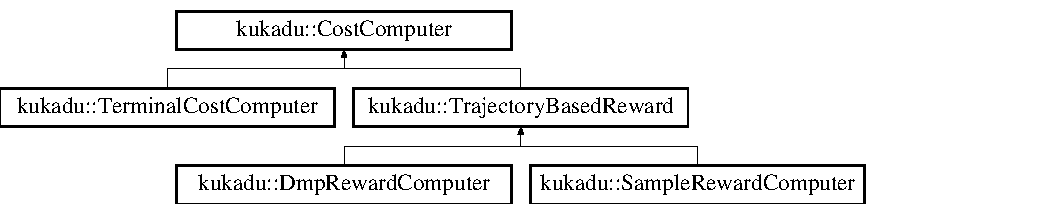
\includegraphics[height=2.745098cm]{classkukadu_1_1CostComputer}
\end{center}
\end{figure}
\subsection*{Public Member Functions}
\begin{DoxyCompactItemize}
\item 
virtual double \hyperlink{classkukadu_1_1CostComputer_a8d02974e1f097ac0451f03f535843175}{compute\-Cost} (K\-U\-K\-A\-D\-U\-\_\-\-S\-H\-A\-R\-E\-D\-\_\-\-P\-T\-R$<$ \hyperlink{classkukadu_1_1ControllerResult}{Controller\-Result} $>$ results)=0
\begin{DoxyCompactList}\small\item\em computes cost for a given dmp execution \end{DoxyCompactList}\end{DoxyCompactItemize}


\subsection{Detailed Description}
Interface for reinforcement learning cost function computation used by \hyperlink{classkukadu_1_1DMPReinforcer}{D\-M\-P\-Reinforcer}. 

This class provides the necessary interfaces for the cost function computation 

\subsection{Member Function Documentation}
\hypertarget{classkukadu_1_1CostComputer_a8d02974e1f097ac0451f03f535843175}{\index{kukadu\-::\-Cost\-Computer@{kukadu\-::\-Cost\-Computer}!compute\-Cost@{compute\-Cost}}
\index{compute\-Cost@{compute\-Cost}!kukadu::CostComputer@{kukadu\-::\-Cost\-Computer}}
\subsubsection[{compute\-Cost}]{\setlength{\rightskip}{0pt plus 5cm}virtual double kukadu\-::\-Cost\-Computer\-::compute\-Cost (
\begin{DoxyParamCaption}
\item[{K\-U\-K\-A\-D\-U\-\_\-\-S\-H\-A\-R\-E\-D\-\_\-\-P\-T\-R$<$ {\bf Controller\-Result} $>$}]{results}
\end{DoxyParamCaption}
)\hspace{0.3cm}{\ttfamily [pure virtual]}}}\label{classkukadu_1_1CostComputer_a8d02974e1f097ac0451f03f535843175}


computes cost for a given dmp execution 


\begin{DoxyParams}{Parameters}
{\em results} & measured results of the last dmp execution \\
\hline
\end{DoxyParams}


Implemented in \hyperlink{classkukadu_1_1TrajectoryBasedReward_a320c223ada03c976b2c545203d1b26d8}{kukadu\-::\-Trajectory\-Based\-Reward}, and \hyperlink{classkukadu_1_1TerminalCostComputer_aec0329f108e413d004139f5da01f04e5}{kukadu\-::\-Terminal\-Cost\-Computer}.



The documentation for this class was generated from the following file\-:\begin{DoxyCompactItemize}
\item 
/home/c7031109/iis\-\_\-robot\-\_\-sw/iis\-\_\-catkin\-\_\-ws/src/kukadu/include/kukadu/learning/rl/costcomputer.\-hpp\end{DoxyCompactItemize}

\hypertarget{classkukadu_1_1CustomSet}{\section{kukadu\-:\-:Custom\-Set Class Reference}
\label{classkukadu_1_1CustomSet}\index{kukadu\-::\-Custom\-Set@{kukadu\-::\-Custom\-Set}}
}
Inheritance diagram for kukadu\-:\-:Custom\-Set\-:\begin{figure}[H]
\begin{center}
\leavevmode
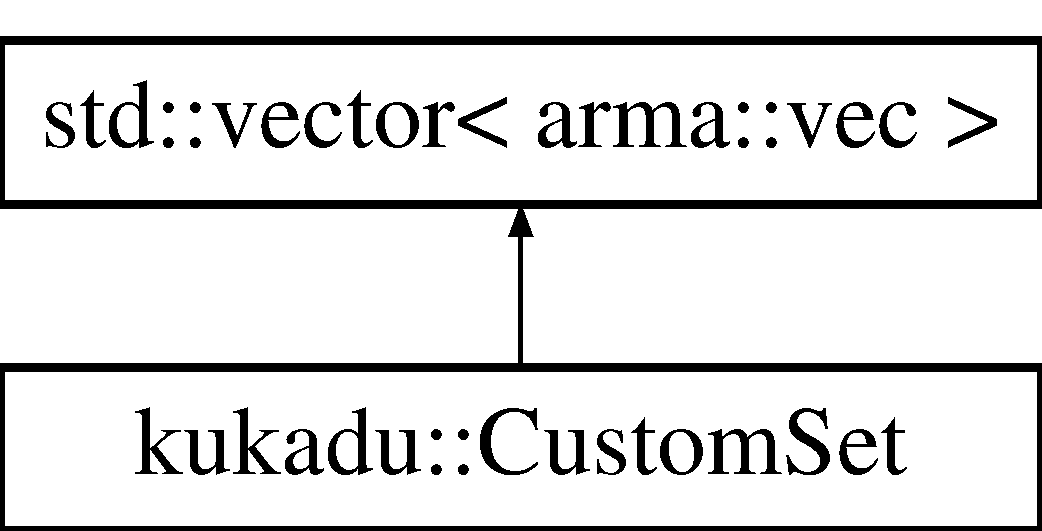
\includegraphics[height=2.000000cm]{classkukadu_1_1CustomSet}
\end{center}
\end{figure}
\subsection*{Public Member Functions}
\begin{DoxyCompactItemize}
\item 
\hypertarget{classkukadu_1_1CustomSet_aba3114ce0bb11303b44a9781650e24e2}{std\-::pair$<$ std\-::vector\\*
$<$ arma\-::vec $>$\-::iterator, int $>$ {\bfseries insert} (arma\-::vec vec1)}\label{classkukadu_1_1CustomSet_aba3114ce0bb11303b44a9781650e24e2}

\item 
\hypertarget{classkukadu_1_1CustomSet_a5339205bb45abd8c4a3ea927c000aa2e}{std\-::pair$<$ std\-::vector\\*
$<$ arma\-::vec $>$\-::iterator, int $>$ {\bfseries find} (arma\-::vec vec1)}\label{classkukadu_1_1CustomSet_a5339205bb45abd8c4a3ea927c000aa2e}

\end{DoxyCompactItemize}


The documentation for this class was generated from the following files\-:\begin{DoxyCompactItemize}
\item 
/home/c7031109/iis\-\_\-robot\-\_\-sw/iis\-\_\-catkin\-\_\-ws/src/kukadu/include/kukadu/utils/customset.\-hpp\item 
/home/c7031109/iis\-\_\-robot\-\_\-sw/iis\-\_\-catkin\-\_\-ws/src/kukadu/src/utils/customset.\-cpp\end{DoxyCompactItemize}

\hypertarget{classkukadu_1_1DestroyableObject}{\section{kukadu\-:\-:Destroyable\-Object Class Reference}
\label{classkukadu_1_1DestroyableObject}\index{kukadu\-::\-Destroyable\-Object@{kukadu\-::\-Destroyable\-Object}}
}


Interface defining a callback function.  




{\ttfamily \#include $<$destroyableobject.\-hpp$>$}

Inheritance diagram for kukadu\-:\-:Destroyable\-Object\-:\begin{figure}[H]
\begin{center}
\leavevmode
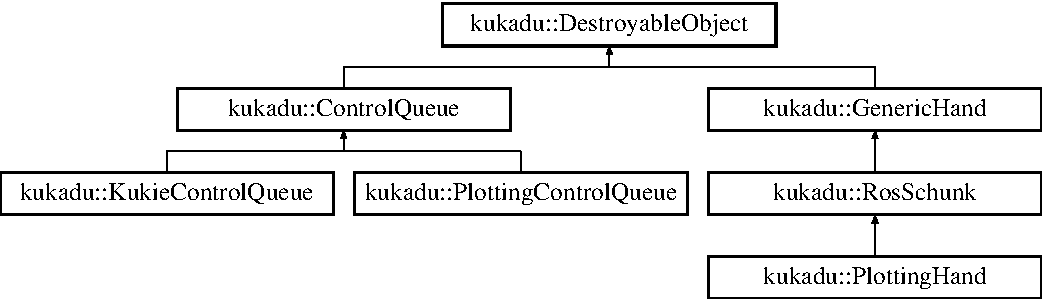
\includegraphics[height=4.000000cm]{classkukadu_1_1DestroyableObject}
\end{center}
\end{figure}
\subsection*{Public Member Functions}
\begin{DoxyCompactItemize}
\item 
virtual void \hyperlink{classkukadu_1_1DestroyableObject_a9e490cfa46af84690eb5ff0682df986c}{safely\-Destroy} ()=0
\begin{DoxyCompactList}\small\item\em Method is called whenever destroy event occurs and ensures safe and clean termination of the programm (e.\-g. stops robot) \end{DoxyCompactList}\end{DoxyCompactItemize}


\subsection{Detailed Description}
Interface defining a callback function. 

The specified callback function should be called whenever unexpected behaviour during robot execution occurs. This is used to handle this execption in a controlled way. 

\subsection{Member Function Documentation}
\hypertarget{classkukadu_1_1DestroyableObject_a9e490cfa46af84690eb5ff0682df986c}{\index{kukadu\-::\-Destroyable\-Object@{kukadu\-::\-Destroyable\-Object}!safely\-Destroy@{safely\-Destroy}}
\index{safely\-Destroy@{safely\-Destroy}!kukadu::DestroyableObject@{kukadu\-::\-Destroyable\-Object}}
\subsubsection[{safely\-Destroy}]{\setlength{\rightskip}{0pt plus 5cm}virtual void kukadu\-::\-Destroyable\-Object\-::safely\-Destroy (
\begin{DoxyParamCaption}
{}
\end{DoxyParamCaption}
)\hspace{0.3cm}{\ttfamily [pure virtual]}}}\label{classkukadu_1_1DestroyableObject_a9e490cfa46af84690eb5ff0682df986c}


Method is called whenever destroy event occurs and ensures safe and clean termination of the programm (e.\-g. stops robot) 



Implemented in \hyperlink{classkukadu_1_1KukieControlQueue_a39da1e622d39d7870c9d0e802d5afa4b}{kukadu\-::\-Kukie\-Control\-Queue}, \hyperlink{classkukadu_1_1PlottingControlQueue_ae15b42e3d6b4b98bc2e470ff3ab3f7ea}{kukadu\-::\-Plotting\-Control\-Queue}, \hyperlink{classkukadu_1_1RosSchunk_a3a50fb0908f1fac2151934ba9759825c}{kukadu\-::\-Ros\-Schunk}, and \hyperlink{classkukadu_1_1PlottingHand_aa57430413a6c183592debe8c881c8520}{kukadu\-::\-Plotting\-Hand}.



The documentation for this class was generated from the following file\-:\begin{DoxyCompactItemize}
\item 
/home/c7031109/iis\-\_\-robot\-\_\-sw/iis\-\_\-catkin\-\_\-ws/src/kukadu/include/kukadu/utils/destroyableobject.\-hpp\end{DoxyCompactItemize}

\hypertarget{classkukadu_1_1DictionaryTrajectory}{\section{kukadu\-:\-:Dictionary\-Trajectory Class Reference}
\label{classkukadu_1_1DictionaryTrajectory}\index{kukadu\-::\-Dictionary\-Trajectory@{kukadu\-::\-Dictionary\-Trajectory}}
}
Inheritance diagram for kukadu\-:\-:Dictionary\-Trajectory\-:\begin{figure}[H]
\begin{center}
\leavevmode
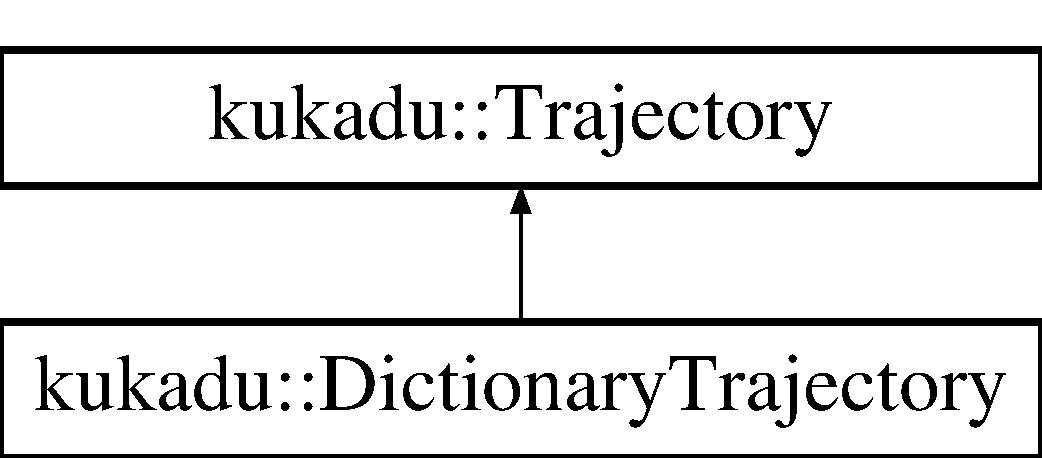
\includegraphics[height=2.000000cm]{classkukadu_1_1DictionaryTrajectory}
\end{center}
\end{figure}
\subsection*{Public Member Functions}
\begin{DoxyCompactItemize}
\item 
\hypertarget{classkukadu_1_1DictionaryTrajectory_a870747d3c8944989b77d1eef393c95aa}{{\bfseries Dictionary\-Trajectory} (const \hyperlink{classkukadu_1_1DictionaryTrajectory}{Dictionary\-Trajectory} \&copy)}\label{classkukadu_1_1DictionaryTrajectory_a870747d3c8944989b77d1eef393c95aa}

\item 
\hypertarget{classkukadu_1_1DictionaryTrajectory_ac86c379b5928d442991b7bf16a9dabc5}{{\bfseries Dictionary\-Trajectory} (std\-::string base\-Folder, double az, double bz)}\label{classkukadu_1_1DictionaryTrajectory_ac86c379b5928d442991b7bf16a9dabc5}

\item 
\hypertarget{classkukadu_1_1DictionaryTrajectory_ad6e50b83eca9a28f4f1f491aca0adced}{void {\bfseries set\-Tmax} (double tmax)}\label{classkukadu_1_1DictionaryTrajectory_ad6e50b83eca9a28f4f1f491aca0adced}

\item 
\hypertarget{classkukadu_1_1DictionaryTrajectory_a0a8f57d5f4f0928a86e33c72b4b13b72}{void {\bfseries set\-Coefficients} (std\-::vector$<$ arma\-::vec $>$ coeffs)}\label{classkukadu_1_1DictionaryTrajectory_a0a8f57d5f4f0928a86e33c72b4b13b72}

\item 
\hypertarget{classkukadu_1_1DictionaryTrajectory_adda7370fe6219f6ebc338dfd069eb82d}{int {\bfseries get\-Degrees\-Of\-Freedom} () const }\label{classkukadu_1_1DictionaryTrajectory_adda7370fe6219f6ebc338dfd069eb82d}

\item 
\hypertarget{classkukadu_1_1DictionaryTrajectory_a7555c07b4021fc812273ccbcfbf687e4}{int {\bfseries operator==} (\hyperlink{classkukadu_1_1DictionaryTrajectory}{Dictionary\-Trajectory} const \&comp) const }\label{classkukadu_1_1DictionaryTrajectory_a7555c07b4021fc812273ccbcfbf687e4}

\item 
\hypertarget{classkukadu_1_1DictionaryTrajectory_ac712e5e1bb0ffdeff574b215adbf483c}{double {\bfseries get\-Tmax} ()}\label{classkukadu_1_1DictionaryTrajectory_ac712e5e1bb0ffdeff574b215adbf483c}

\item 
\hypertarget{classkukadu_1_1DictionaryTrajectory_a271c61b9017bc3bab7c8743197680310}{arma\-::vec {\bfseries get\-Starting\-Pos} ()}\label{classkukadu_1_1DictionaryTrajectory_a271c61b9017bc3bab7c8743197680310}

\item 
\hypertarget{classkukadu_1_1DictionaryTrajectory_ab118502bdf3cb95cc52f7dc640572deb}{std\-::vector$<$ arma\-::vec $>$ {\bfseries get\-Coefficients} ()}\label{classkukadu_1_1DictionaryTrajectory_ab118502bdf3cb95cc52f7dc640572deb}

\item 
\hypertarget{classkukadu_1_1DictionaryTrajectory_a4d1fd2fcff1e7a696976a2b50bdb1a9a}{std\-::vector$<$ \hyperlink{classkukadu_1_1QueryPoint}{Query\-Point} $>$ {\bfseries get\-Query\-Points} ()}\label{classkukadu_1_1DictionaryTrajectory_a4d1fd2fcff1e7a696976a2b50bdb1a9a}

\item 
\hypertarget{classkukadu_1_1DictionaryTrajectory_a4bdb28bd8c9bb18572f8b1d78c683d02}{K\-U\-K\-A\-D\-U\-\_\-\-S\-H\-A\-R\-E\-D\-\_\-\-P\-T\-R$<$ \hyperlink{classkukadu_1_1Trajectory}{Trajectory} $>$ {\bfseries copy} ()}\label{classkukadu_1_1DictionaryTrajectory_a4bdb28bd8c9bb18572f8b1d78c683d02}

\end{DoxyCompactItemize}


The documentation for this class was generated from the following files\-:\begin{DoxyCompactItemize}
\item 
/home/c7031109/iis\-\_\-robot\-\_\-sw/iis\-\_\-catkin\-\_\-ws/src/kukadu/include/kukadu/types/dictionarytrajectory.\-hpp\item 
/home/c7031109/iis\-\_\-robot\-\_\-sw/iis\-\_\-catkin\-\_\-ws/src/kukadu/src/types/dictionarytrajectory.\-cpp\end{DoxyCompactItemize}

\hypertarget{classkukadu_1_1Dmp}{\section{kukadu\-:\-:Dmp Class Reference}
\label{classkukadu_1_1Dmp}\index{kukadu\-::\-Dmp@{kukadu\-::\-Dmp}}
}
Inheritance diagram for kukadu\-:\-:Dmp\-:\begin{figure}[H]
\begin{center}
\leavevmode
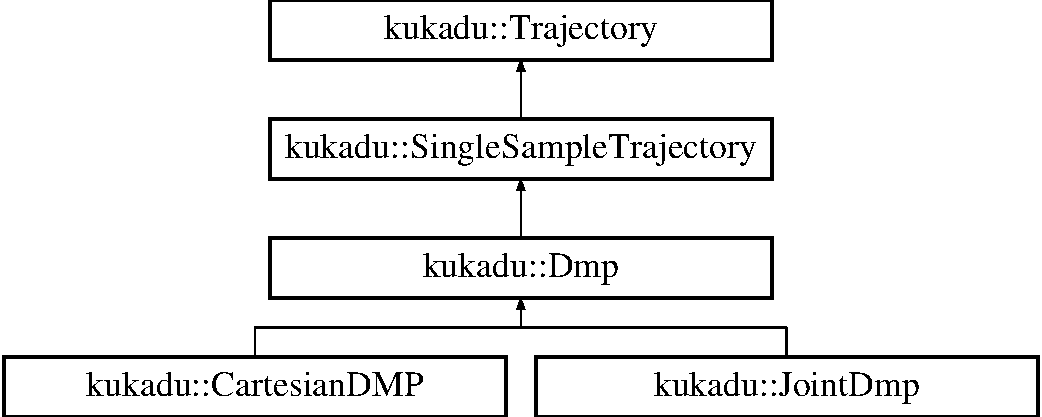
\includegraphics[height=4.000000cm]{classkukadu_1_1Dmp}
\end{center}
\end{figure}
\subsection*{Public Member Functions}
\begin{DoxyCompactItemize}
\item 
\hypertarget{classkukadu_1_1Dmp_a780c7d0ea48cc2dfaac10dbc8db9ecc6}{{\bfseries Dmp} (const \hyperlink{classkukadu_1_1Dmp}{Dmp} \&copy)}\label{classkukadu_1_1Dmp_a780c7d0ea48cc2dfaac10dbc8db9ecc6}

\item 
\hypertarget{classkukadu_1_1Dmp_a087cd38d5201e57f7404c6971bef1884}{{\bfseries Dmp} (std\-::string dmp\-File)}\label{classkukadu_1_1Dmp_a087cd38d5201e57f7404c6971bef1884}

\item 
\hypertarget{classkukadu_1_1Dmp_a0a490a4a7272808abd3f27ba40cb3ffd}{{\bfseries Dmp} (arma\-::vec supervised\-Ts, std\-::vector$<$ arma\-::vec $>$ sample\-Ys, std\-::vector$<$ arma\-::vec $>$ fit\-Ys, std\-::vector$<$ arma\-::vec $>$ dmp\-Coeffs, std\-::vector$<$ \hyperlink{classkukadu_1_1DMPBase}{D\-M\-P\-Base} $>$ dmp\-Base, std\-::vector$<$ arma\-::mat $>$ design\-Matrices, double tau, double az, double bz, double ax, double ac, double dmp\-Step\-Size, double tol\-Abs\-Err, double tol\-Rel\-Err)}\label{classkukadu_1_1Dmp_a0a490a4a7272808abd3f27ba40cb3ffd}

\item 
\hypertarget{classkukadu_1_1Dmp_a8b1adacb0928a62002005de708608621}{{\bfseries Dmp} (arma\-::vec supervised\-Ts, std\-::vector$<$ arma\-::vec $>$ sample\-Ys, std\-::vector$<$ arma\-::vec $>$ fit\-Ys, std\-::vector$<$ arma\-::vec $>$ dmp\-Coeffs, std\-::vector$<$ \hyperlink{classkukadu_1_1DMPBase}{D\-M\-P\-Base} $>$ dmp\-Base, std\-::vector$<$ arma\-::mat $>$ design\-Matrices, double tau, double az, double bz, double ax)}\label{classkukadu_1_1Dmp_a8b1adacb0928a62002005de708608621}

\item 
\hypertarget{classkukadu_1_1Dmp_a67645036f7e1dfb7ff833b8149716c2d}{void {\bfseries serialize} (std\-::string dmp\-File)}\label{classkukadu_1_1Dmp_a67645036f7e1dfb7ff833b8149716c2d}

\item 
\hypertarget{classkukadu_1_1Dmp_ab81d2e2b6f51744caff8714824afb940}{int {\bfseries get\-Sample\-Count} ()}\label{classkukadu_1_1Dmp_ab81d2e2b6f51744caff8714824afb940}

\item 
\hypertarget{classkukadu_1_1Dmp_ab5256cb887386b5fd48a88e60a14e1d6}{double {\bfseries get\-Y0} (int freedom\-Idx)}\label{classkukadu_1_1Dmp_ab5256cb887386b5fd48a88e60a14e1d6}

\item 
\hypertarget{classkukadu_1_1Dmp_a1a552adfe0f620b5c34e05ecf56fd55f}{double {\bfseries get\-Dy0} (int freedom\-Idx)}\label{classkukadu_1_1Dmp_a1a552adfe0f620b5c34e05ecf56fd55f}

\item 
\hypertarget{classkukadu_1_1Dmp_a7d16db0cc1e7aadb52e88b9ce88ed013}{double {\bfseries get\-Ddy0} (int freedom\-Idx)}\label{classkukadu_1_1Dmp_a7d16db0cc1e7aadb52e88b9ce88ed013}

\item 
\hypertarget{classkukadu_1_1Dmp_a1b7816ff8f66155afad0a50f9cf40ab0}{double {\bfseries get\-G} (int freedom\-Idx)}\label{classkukadu_1_1Dmp_a1b7816ff8f66155afad0a50f9cf40ab0}

\item 
\hypertarget{classkukadu_1_1Dmp_ae2c58371b5c9846a8d4e5a6145a5b4a8}{arma\-::vec {\bfseries get\-Y0} ()}\label{classkukadu_1_1Dmp_ae2c58371b5c9846a8d4e5a6145a5b4a8}

\item 
\hypertarget{classkukadu_1_1Dmp_a507c50bd598249260b23368ed5ea88c8}{arma\-::vec {\bfseries get\-Dy0} ()}\label{classkukadu_1_1Dmp_a507c50bd598249260b23368ed5ea88c8}

\item 
\hypertarget{classkukadu_1_1Dmp_a625b8794d3e59632412f76d447ccc430}{arma\-::vec {\bfseries get\-Ddy0} ()}\label{classkukadu_1_1Dmp_a625b8794d3e59632412f76d447ccc430}

\item 
\hypertarget{classkukadu_1_1Dmp_ac8c841b12e4eb2678424d96c6dbbb5bc}{arma\-::vec {\bfseries get\-G} ()}\label{classkukadu_1_1Dmp_ac8c841b12e4eb2678424d96c6dbbb5bc}

\item 
\hypertarget{classkukadu_1_1Dmp_a4b477fea8132d45d50617d9027f55634}{std\-::vector$<$ arma\-::vec $>$ {\bfseries get\-Coefficients} ()}\label{classkukadu_1_1Dmp_a4b477fea8132d45d50617d9027f55634}

\item 
\hypertarget{classkukadu_1_1Dmp_ace27ff809c779f83daf1fd903636a332}{void {\bfseries set\-Coefficients} (std\-::vector$<$ arma\-::vec $>$ coeffs)}\label{classkukadu_1_1Dmp_ace27ff809c779f83daf1fd903636a332}

\item 
\hypertarget{classkukadu_1_1Dmp_aec1043e1b9eda2418848eca83e3b7ae1}{std\-::vector$<$ arma\-::vec $>$ {\bfseries get\-Dmp\-Coeffs} ()}\label{classkukadu_1_1Dmp_aec1043e1b9eda2418848eca83e3b7ae1}

\item 
\hypertarget{classkukadu_1_1Dmp_aa9074177aa8d7272d83456cf9aafde4c}{std\-::vector$<$ arma\-::vec $>$ {\bfseries get\-Fit\-Ys} ()}\label{classkukadu_1_1Dmp_aa9074177aa8d7272d83456cf9aafde4c}

\item 
\hypertarget{classkukadu_1_1Dmp_a6feb8dc33dc6b8b6cd032fa3b234dec0}{void {\bfseries set\-Dmp\-Coeffs} (std\-::vector$<$ arma\-::vec $>$ coeffs)}\label{classkukadu_1_1Dmp_a6feb8dc33dc6b8b6cd032fa3b234dec0}

\item 
\hypertarget{classkukadu_1_1Dmp_acf8b80c2993b1588d5aeab638480222d}{arma\-::vec {\bfseries get\-Dmp\-Coeffs} (int freedom\-Idx)}\label{classkukadu_1_1Dmp_acf8b80c2993b1588d5aeab638480222d}

\item 
\hypertarget{classkukadu_1_1Dmp_ad8cbaf545f773e2b347521c4d4f81972}{arma\-::mat {\bfseries get\-Design\-Matrix} (int freedom\-Idx)}\label{classkukadu_1_1Dmp_ad8cbaf545f773e2b347521c4d4f81972}

\item 
\hypertarget{classkukadu_1_1Dmp_aaa2bbfc5b9683d38c7dc3cae4fd66d35}{int {\bfseries get\-Design\-Matrix\-Count} ()}\label{classkukadu_1_1Dmp_aaa2bbfc5b9683d38c7dc3cae4fd66d35}

\item 
\hypertarget{classkukadu_1_1Dmp_a22ef512c5a0fb56808212c18eeabb4f6}{std\-::vector$<$ \hyperlink{classkukadu_1_1DMPBase}{D\-M\-P\-Base} $>$ {\bfseries get\-Dmp\-Base} ()}\label{classkukadu_1_1Dmp_a22ef512c5a0fb56808212c18eeabb4f6}

\item 
\hypertarget{classkukadu_1_1Dmp_a1ec31b0b369dac93fe7b4913ab8863db}{double {\bfseries get\-Delta\-T\-By\-Idx} (int idx)}\label{classkukadu_1_1Dmp_a1ec31b0b369dac93fe7b4913ab8863db}

\item 
\hypertarget{classkukadu_1_1Dmp_a787076c787e247bc14c07e738617e5f6}{double {\bfseries get\-Tau} ()}\label{classkukadu_1_1Dmp_a787076c787e247bc14c07e738617e5f6}

\item 
\hypertarget{classkukadu_1_1Dmp_aaec08d60cac323f41ffdad60c0218ea9}{double {\bfseries get\-Az} ()}\label{classkukadu_1_1Dmp_aaec08d60cac323f41ffdad60c0218ea9}

\item 
\hypertarget{classkukadu_1_1Dmp_a25805f30ba5af184d2cb3f228d74bc47}{double {\bfseries get\-Bz} ()}\label{classkukadu_1_1Dmp_a25805f30ba5af184d2cb3f228d74bc47}

\item 
\hypertarget{classkukadu_1_1Dmp_afecc2e30b16281ae8e46fbd0797ba9da}{double {\bfseries get\-Ax} ()}\label{classkukadu_1_1Dmp_afecc2e30b16281ae8e46fbd0797ba9da}

\item 
\hypertarget{classkukadu_1_1Dmp_aa88cf46b01a29848c307ab8c66cd3c1e}{double {\bfseries get\-Step\-Size} ()}\label{classkukadu_1_1Dmp_aa88cf46b01a29848c307ab8c66cd3c1e}

\item 
\hypertarget{classkukadu_1_1Dmp_ae72973627e7443f6b98b07891fba2705}{double {\bfseries get\-Tol\-Abs\-Err} ()}\label{classkukadu_1_1Dmp_ae72973627e7443f6b98b07891fba2705}

\item 
\hypertarget{classkukadu_1_1Dmp_a8a90b4bf9c8acf5a3aeaeb2c82671929}{double {\bfseries get\-Tol\-Rel\-Err} ()}\label{classkukadu_1_1Dmp_a8a90b4bf9c8acf5a3aeaeb2c82671929}

\item 
\hypertarget{classkukadu_1_1Dmp_aa7423b1cd8096790cc6162e7ecfb604b}{double {\bfseries get\-Tmax} ()}\label{classkukadu_1_1Dmp_aa7423b1cd8096790cc6162e7ecfb604b}

\item 
\hypertarget{classkukadu_1_1Dmp_a90ba745176c444fb74bfd24722ee8f60}{void {\bfseries set\-Tmax} (double tmax)}\label{classkukadu_1_1Dmp_a90ba745176c444fb74bfd24722ee8f60}

\item 
\hypertarget{classkukadu_1_1Dmp_ac64f37f77911ba0d6e67ea4041601dd8}{virtual bool {\bfseries is\-Cartesian} ()=0}\label{classkukadu_1_1Dmp_ac64f37f77911ba0d6e67ea4041601dd8}

\item 
\hypertarget{classkukadu_1_1Dmp_ad944a1f4b2e1857c390f3ab42d64d59b}{int {\bfseries operator==} (K\-U\-K\-A\-D\-U\-\_\-\-S\-H\-A\-R\-E\-D\-\_\-\-P\-T\-R$<$ \hyperlink{classkukadu_1_1Dmp}{Dmp} $>$ const \&comp) const }\label{classkukadu_1_1Dmp_ad944a1f4b2e1857c390f3ab42d64d59b}

\end{DoxyCompactItemize}
\subsection*{Protected Attributes}
\begin{DoxyCompactItemize}
\item 
\hypertarget{classkukadu_1_1Dmp_af0966b32d5f703b6c59a24332f994715}{double {\bfseries dmp\-Step\-Size}}\label{classkukadu_1_1Dmp_af0966b32d5f703b6c59a24332f994715}

\item 
\hypertarget{classkukadu_1_1Dmp_a1f5e7194bf55d600d9eb1e7447ed552d}{std\-::vector$<$ arma\-::vec $>$ {\bfseries fit\-Ys}}\label{classkukadu_1_1Dmp_a1f5e7194bf55d600d9eb1e7447ed552d}

\end{DoxyCompactItemize}


The documentation for this class was generated from the following files\-:\begin{DoxyCompactItemize}
\item 
/home/c7031109/iis\-\_\-robot\-\_\-sw/iis\-\_\-catkin\-\_\-ws/src/kukadu/include/kukadu/types/dmp.\-hpp\item 
/home/c7031109/iis\-\_\-robot\-\_\-sw/iis\-\_\-catkin\-\_\-ws/src/kukadu/src/types/dmp.\-cpp\end{DoxyCompactItemize}

\hypertarget{classkukadu_1_1DMPBase}{\section{kukadu\-:\-:D\-M\-P\-Base Class Reference}
\label{classkukadu_1_1DMPBase}\index{kukadu\-::\-D\-M\-P\-Base@{kukadu\-::\-D\-M\-P\-Base}}
}
\subsection*{Public Member Functions}
\begin{DoxyCompactItemize}
\item 
\hypertarget{classkukadu_1_1DMPBase_a4a752a432b73e33eb50ab35b6109872c}{{\bfseries D\-M\-P\-Base} (float my, std\-::vector$<$ double $>$ sigmas)}\label{classkukadu_1_1DMPBase_a4a752a432b73e33eb50ab35b6109872c}

\item 
\hypertarget{classkukadu_1_1DMPBase_a2b25a18ef07e4c2202246aa1f142b0b7}{float {\bfseries get\-My} ()}\label{classkukadu_1_1DMPBase_a2b25a18ef07e4c2202246aa1f142b0b7}

\item 
\hypertarget{classkukadu_1_1DMPBase_af65d964c6a5ecd9f22961cbad41bc847}{std\-::vector$<$ double $>$ {\bfseries get\-Sigmas} ()}\label{classkukadu_1_1DMPBase_af65d964c6a5ecd9f22961cbad41bc847}

\item 
\hypertarget{classkukadu_1_1DMPBase_abf6e42c62e3d1dc00009b0576c85608e}{int {\bfseries operator==} (\hyperlink{classkukadu_1_1DMPBase}{D\-M\-P\-Base} const \&comp) const }\label{classkukadu_1_1DMPBase_abf6e42c62e3d1dc00009b0576c85608e}

\end{DoxyCompactItemize}


The documentation for this class was generated from the following files\-:\begin{DoxyCompactItemize}
\item 
/home/c7031109/iis\-\_\-robot\-\_\-sw/iis\-\_\-catkin\-\_\-ws/src/kukadu/include/kukadu/types/dmpbase.\-hpp\item 
/home/c7031109/iis\-\_\-robot\-\_\-sw/iis\-\_\-catkin\-\_\-ws/src/kukadu/src/types/dmpbase.\-cpp\end{DoxyCompactItemize}

\hypertarget{classkukadu_1_1DMPExecutor}{\section{kukadu\-:\-:D\-M\-P\-Executor Class Reference}
\label{classkukadu_1_1DMPExecutor}\index{kukadu\-::\-D\-M\-P\-Executor@{kukadu\-::\-D\-M\-P\-Executor}}
}


This class is responsible for dmp execution.  




{\ttfamily \#include $<$dmpexecutor.\-hpp$>$}

Inheritance diagram for kukadu\-:\-:D\-M\-P\-Executor\-:\begin{figure}[H]
\begin{center}
\leavevmode
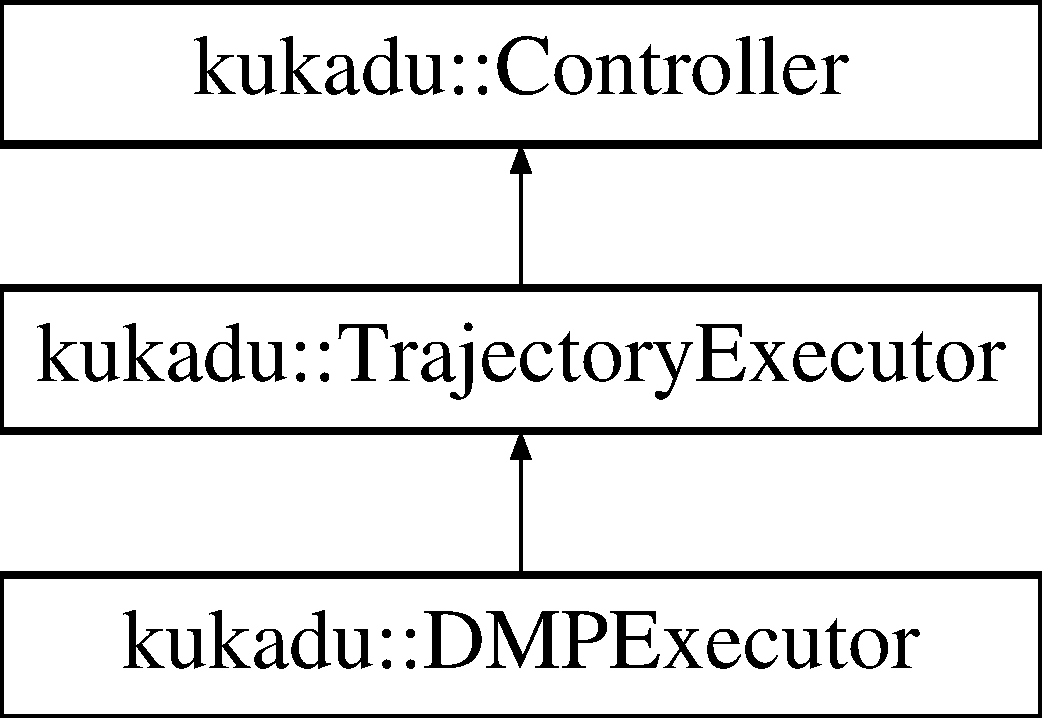
\includegraphics[height=3.000000cm]{classkukadu_1_1DMPExecutor}
\end{center}
\end{figure}
\subsection*{Public Member Functions}
\begin{DoxyCompactItemize}
\item 
\hyperlink{classkukadu_1_1DMPExecutor_a373f61b9ca50f365edbbbe2c5cfab93d}{D\-M\-P\-Executor} (K\-U\-K\-A\-D\-U\-\_\-\-S\-H\-A\-R\-E\-D\-\_\-\-P\-T\-R$<$ \hyperlink{classkukadu_1_1Dmp}{Dmp} $>$ dmp, K\-U\-K\-A\-D\-U\-\_\-\-S\-H\-A\-R\-E\-D\-\_\-\-P\-T\-R$<$ \hyperlink{classkukadu_1_1ControlQueue}{Control\-Queue} $>$ exec\-Queue)
\begin{DoxyCompactList}\small\item\em constructor \end{DoxyCompactList}\item 
\hypertarget{classkukadu_1_1DMPExecutor_aee2adcadd6e701b75fb7b94b17f083ab}{{\bfseries D\-M\-P\-Executor} (K\-U\-K\-A\-D\-U\-\_\-\-S\-H\-A\-R\-E\-D\-\_\-\-P\-T\-R$<$ \hyperlink{classkukadu_1_1Trajectory}{Trajectory} $>$ dmp, K\-U\-K\-A\-D\-U\-\_\-\-S\-H\-A\-R\-E\-D\-\_\-\-P\-T\-R$<$ \hyperlink{classkukadu_1_1ControlQueue}{Control\-Queue} $>$ exec\-Queue)}\label{classkukadu_1_1DMPExecutor_aee2adcadd6e701b75fb7b94b17f083ab}

\item 
\hypertarget{classkukadu_1_1DMPExecutor_a354052531aca0fa4fbc35f6f075a7763}{{\bfseries D\-M\-P\-Executor} (K\-U\-K\-A\-D\-U\-\_\-\-S\-H\-A\-R\-E\-D\-\_\-\-P\-T\-R$<$ \hyperlink{classkukadu_1_1Dmp}{Dmp} $>$ dmp, K\-U\-K\-A\-D\-U\-\_\-\-S\-H\-A\-R\-E\-D\-\_\-\-P\-T\-R$<$ \hyperlink{classkukadu_1_1ControlQueue}{Control\-Queue} $>$ exec\-Queue, int suppress\-Messages)}\label{classkukadu_1_1DMPExecutor_a354052531aca0fa4fbc35f6f075a7763}

\item 
\hypertarget{classkukadu_1_1DMPExecutor_a97054e488e997d275cdcc8d58554a3e6}{int {\bfseries uses\-External\-Error} ()}\label{classkukadu_1_1DMPExecutor_a97054e488e997d275cdcc8d58554a3e6}

\item 
\hypertarget{classkukadu_1_1DMPExecutor_aa67aae8df58ef660f694a0c322fa251e}{void {\bfseries destroy\-Integration} ()}\label{classkukadu_1_1DMPExecutor_aa67aae8df58ef660f694a0c322fa251e}

\item 
\hypertarget{classkukadu_1_1DMPExecutor_a30488907c4a7f95040137aaa22f7783d}{void {\bfseries initialize\-Integration\-Quat} ()}\label{classkukadu_1_1DMPExecutor_a30488907c4a7f95040137aaa22f7783d}

\item 
\hypertarget{classkukadu_1_1DMPExecutor_af6bdcf008a271ebaf971e538ee7de962}{void {\bfseries use\-External\-Error} (int external)}\label{classkukadu_1_1DMPExecutor_af6bdcf008a271ebaf971e538ee7de962}

\item 
\hypertarget{classkukadu_1_1DMPExecutor_a0f61c96beb3e2d2d263d2de02da6afa4}{void {\bfseries set\-External\-Error} (double error)}\label{classkukadu_1_1DMPExecutor_a0f61c96beb3e2d2d263d2de02da6afa4}

\item 
\hypertarget{classkukadu_1_1DMPExecutor_a48f9f9b4b12ebce4423c0258be1c6eb5}{void {\bfseries enable\-Max\-Force\-Mode} (double max\-Abs\-Force, double max\-X\-Force, double max\-Y\-Force, double max\-Z\-Force)}\label{classkukadu_1_1DMPExecutor_a48f9f9b4b12ebce4423c0258be1c6eb5}

\item 
\hypertarget{classkukadu_1_1DMPExecutor_a4278c7a3e74556a5e2c40a7602743852}{void {\bfseries do\-Roll\-Back\-On\-Max\-Force\-Event} (bool do\-Rollback)}\label{classkukadu_1_1DMPExecutor_a4278c7a3e74556a5e2c40a7602743852}

\item 
\hypertarget{classkukadu_1_1DMPExecutor_a05c30d4373ffdedf10711d66ca7e979e}{void {\bfseries set\-Trajectory} (K\-U\-K\-A\-D\-U\-\_\-\-S\-H\-A\-R\-E\-D\-\_\-\-P\-T\-R$<$ \hyperlink{classkukadu_1_1Trajectory}{Trajectory} $>$ traj)}\label{classkukadu_1_1DMPExecutor_a05c30d4373ffdedf10711d66ca7e979e}

\item 
\hypertarget{classkukadu_1_1DMPExecutor_a3c6748e4c5731fa8d3721fb703cb8ec8}{void {\bfseries initialize\-Integration} (double t\-Start, double tol\-Abs\-Err, double tol\-Rel\-Err)}\label{classkukadu_1_1DMPExecutor_a3c6748e4c5731fa8d3721fb703cb8ec8}

\item 
\hypertarget{classkukadu_1_1DMPExecutor_a35e69b1d2f636f5ba9b7eb596c720aa4}{void {\bfseries construct} (K\-U\-K\-A\-D\-U\-\_\-\-S\-H\-A\-R\-E\-D\-\_\-\-P\-T\-R$<$ \hyperlink{classkukadu_1_1Dmp}{Dmp} $>$ dmp, K\-U\-K\-A\-D\-U\-\_\-\-S\-H\-A\-R\-E\-D\-\_\-\-P\-T\-R$<$ \hyperlink{classkukadu_1_1ControlQueue}{Control\-Queue} $>$ exec\-Queue, int suppress\-Messages)}\label{classkukadu_1_1DMPExecutor_a35e69b1d2f636f5ba9b7eb596c720aa4}

\item 
\hypertarget{classkukadu_1_1DMPExecutor_afefa7096a8b289cbd80c46662fbf0cad}{void {\bfseries set\-Rollback\-Time} (double rollback\-Time)}\label{classkukadu_1_1DMPExecutor_afefa7096a8b289cbd80c46662fbf0cad}

\item 
\hypertarget{classkukadu_1_1DMPExecutor_aa346971808b1383e7b0e65f1e611e1ed}{virtual bool {\bfseries requires\-Grasp} ()}\label{classkukadu_1_1DMPExecutor_aa346971808b1383e7b0e65f1e611e1ed}

\item 
\hypertarget{classkukadu_1_1DMPExecutor_ad8949f9211cc71dfc85a49baddc22724}{virtual bool {\bfseries produces\-Grasp} ()}\label{classkukadu_1_1DMPExecutor_ad8949f9211cc71dfc85a49baddc22724}

\item 
\hypertarget{classkukadu_1_1DMPExecutor_af3ea91620f3c2a7686fd56a2df6c9dd1}{double {\bfseries get\-External\-Error} ()}\label{classkukadu_1_1DMPExecutor_af3ea91620f3c2a7686fd56a2df6c9dd1}

\item 
\hypertarget{classkukadu_1_1DMPExecutor_adb5e00c9c60ffddee9e1b0e019a4ee12}{arma\-::vec {\bfseries do\-Integration\-Step} (double ac)}\label{classkukadu_1_1DMPExecutor_adb5e00c9c60ffddee9e1b0e019a4ee12}

\item 
\hypertarget{classkukadu_1_1DMPExecutor_a6f33217d4d3af41fbb58c2d2a394d397}{K\-U\-K\-A\-D\-U\-\_\-\-S\-H\-A\-R\-E\-D\-\_\-\-P\-T\-R\\*
$<$ \hyperlink{classkukadu_1_1ControllerResult}{Controller\-Result} $>$ {\bfseries execute\-Trajectory} ()}\label{classkukadu_1_1DMPExecutor_a6f33217d4d3af41fbb58c2d2a394d397}

\item 
\hypertarget{classkukadu_1_1DMPExecutor_a7e0a8b15b047b3781e3185ceb9922e0e}{K\-U\-K\-A\-D\-U\-\_\-\-S\-H\-A\-R\-E\-D\-\_\-\-P\-T\-R\\*
$<$ \hyperlink{classkukadu_1_1ControllerResult}{Controller\-Result} $>$ {\bfseries simulate\-Trajectory} ()}\label{classkukadu_1_1DMPExecutor_a7e0a8b15b047b3781e3185ceb9922e0e}

\item 
\hypertarget{classkukadu_1_1DMPExecutor_a7c49950c3d809601a115bab006e8436f}{K\-U\-K\-A\-D\-U\-\_\-\-S\-H\-A\-R\-E\-D\-\_\-\-P\-T\-R\\*
$<$ \hyperlink{classkukadu_1_1ControllerResult}{Controller\-Result} $>$ {\bfseries simulate\-Trajectory} (double t\-Start, double t\-End, double tol\-Abs\-Err, double tol\-Rel\-Err)}\label{classkukadu_1_1DMPExecutor_a7c49950c3d809601a115bab006e8436f}

\item 
\hypertarget{classkukadu_1_1DMPExecutor_a4fe15de30bd8ffac30494b5135afe453}{K\-U\-K\-A\-D\-U\-\_\-\-S\-H\-A\-R\-E\-D\-\_\-\-P\-T\-R\\*
$<$ \hyperlink{classkukadu_1_1ControllerResult}{Controller\-Result} $>$ {\bfseries execute\-Trajectory} (double ac, double t\-Start, double t\-End, double tol\-Abs\-Err, double tol\-Rel\-Err)}\label{classkukadu_1_1DMPExecutor_a4fe15de30bd8ffac30494b5135afe453}

\end{DoxyCompactItemize}
\subsection*{Static Public Attributes}
\begin{DoxyCompactItemize}
\item 
\hypertarget{classkukadu_1_1DMPExecutor_acb1421363d995248e27fa60080cddf81}{static const int {\bfseries S\-I\-M\-U\-L\-A\-T\-E\-\_\-\-D\-M\-P} = 1}\label{classkukadu_1_1DMPExecutor_acb1421363d995248e27fa60080cddf81}

\item 
\hypertarget{classkukadu_1_1DMPExecutor_aa91af5f6472064191b6f53824f25d608}{static const int {\bfseries E\-X\-E\-C\-U\-T\-E\-\_\-\-R\-O\-B\-O\-T} = 2}\label{classkukadu_1_1DMPExecutor_aa91af5f6472064191b6f53824f25d608}

\item 
\hypertarget{classkukadu_1_1DMPExecutor_a4d1aa7315001e2e1ea4ceb22d564f5af}{static const int {\bfseries K\-U\-K\-A\-D\-U\-\_\-\-E\-X\-E\-C\-\_\-\-J\-O\-I\-N\-T} = 1}\label{classkukadu_1_1DMPExecutor_a4d1aa7315001e2e1ea4ceb22d564f5af}

\item 
\hypertarget{classkukadu_1_1DMPExecutor_a411b6f06a54d54edf5dd071530323284}{static const int {\bfseries K\-U\-K\-A\-D\-U\-\_\-\-E\-X\-E\-C\-\_\-\-C\-A\-R\-T} = 2}\label{classkukadu_1_1DMPExecutor_a411b6f06a54d54edf5dd071530323284}

\item 
\hypertarget{classkukadu_1_1DMPExecutor_a7c95850684d0431a4a554b8ecf3dbe62}{static const int {\bfseries I\-G\-N\-O\-R\-E\-\_\-\-F\-O\-R\-C\-E} = -\/1}\label{classkukadu_1_1DMPExecutor_a7c95850684d0431a4a554b8ecf3dbe62}

\end{DoxyCompactItemize}
\subsection*{Protected Member Functions}
\begin{DoxyCompactItemize}
\item 
\hypertarget{classkukadu_1_1DMPExecutor_ab3c4a6e121917b95259aabfcfc348c5b}{void {\bfseries run\-Check\-Max\-Forces} ()}\label{classkukadu_1_1DMPExecutor_ab3c4a6e121917b95259aabfcfc348c5b}

\item 
\hypertarget{classkukadu_1_1DMPExecutor_acc239e5c025fca330fac28590e25721e}{double {\bfseries compute\-Distance} (const arma\-::vec y\-Des, arma\-::vec y\-Curr)}\label{classkukadu_1_1DMPExecutor_acc239e5c025fca330fac28590e25721e}

\item 
\hypertarget{classkukadu_1_1DMPExecutor_ac7930124bda370eed2097e5edbc764cd}{K\-U\-K\-A\-D\-U\-\_\-\-S\-H\-A\-R\-E\-D\-\_\-\-P\-T\-R\\*
$<$ \hyperlink{classkukadu_1_1ControllerResult}{Controller\-Result} $>$ {\bfseries execute\-D\-M\-P} (double t\-Start, double t\-End, double tol\-Abs\-Err, double tol\-Rel\-Err)}\label{classkukadu_1_1DMPExecutor_ac7930124bda370eed2097e5edbc764cd}

\item 
\hypertarget{classkukadu_1_1DMPExecutor_a36fbd2e7ec4aa92d3547716781e92c25}{virtual int {\bfseries func} (double t, const double $\ast$y, double $\ast$f, void $\ast$params)}\label{classkukadu_1_1DMPExecutor_a36fbd2e7ec4aa92d3547716781e92c25}

\item 
\hypertarget{classkukadu_1_1DMPExecutor_a7653d938ffa32d0d6e3401e7db17a87e}{virtual int {\bfseries jac} (double t, const double $\ast$y, double $\ast$dfdy, double $\ast$dfdt, void $\ast$params)}\label{classkukadu_1_1DMPExecutor_a7653d938ffa32d0d6e3401e7db17a87e}

\item 
\hypertarget{classkukadu_1_1DMPExecutor_a8dd322182fb9b37f9a6661865ad66251}{virtual double {\bfseries add\-Term} (double t, const double $\ast$current\-Desired\-Ys, int joint\-Number, K\-U\-K\-A\-D\-U\-\_\-\-S\-H\-A\-R\-E\-D\-\_\-\-P\-T\-R$<$ \hyperlink{classkukadu_1_1ControlQueue}{Control\-Queue} $>$ queue)}\label{classkukadu_1_1DMPExecutor_a8dd322182fb9b37f9a6661865ad66251}

\end{DoxyCompactItemize}
\subsection*{Static Protected Member Functions}
\begin{DoxyCompactItemize}
\item 
\hypertarget{classkukadu_1_1DMPExecutor_ac58ec7a3b98134bcb84aff2b81ffc5c4}{static int {\bfseries static\-\_\-func} (double t, const double y\mbox{[}$\,$\mbox{]}, double f\mbox{[}$\,$\mbox{]}, void $\ast$params)}\label{classkukadu_1_1DMPExecutor_ac58ec7a3b98134bcb84aff2b81ffc5c4}

\item 
\hypertarget{classkukadu_1_1DMPExecutor_a10d8f15cdf66da21fc9e3d4a4d3555b8}{static int {\bfseries static\-\_\-jac} (double t, const double y\mbox{[}$\,$\mbox{]}, double $\ast$dfdy, double dfdt\mbox{[}$\,$\mbox{]}, void $\ast$params)}\label{classkukadu_1_1DMPExecutor_a10d8f15cdf66da21fc9e3d4a4d3555b8}

\end{DoxyCompactItemize}
\subsection*{Protected Attributes}
\begin{DoxyCompactItemize}
\item 
\hypertarget{classkukadu_1_1DMPExecutor_ab2cef867ba977a286257985f499bc08a}{bool {\bfseries do\-Rollback}}\label{classkukadu_1_1DMPExecutor_ab2cef867ba977a286257985f499bc08a}

\item 
\hypertarget{classkukadu_1_1DMPExecutor_a4c8de202dc26fccdabf76efafae9384b}{bool {\bfseries is\-Cartesian}}\label{classkukadu_1_1DMPExecutor_a4c8de202dc26fccdabf76efafae9384b}

\item 
\hypertarget{classkukadu_1_1DMPExecutor_ad81dc828374959b48a1744202dabb648}{bool {\bfseries execution\-Running}}\label{classkukadu_1_1DMPExecutor_ad81dc828374959b48a1744202dabb648}

\item 
\hypertarget{classkukadu_1_1DMPExecutor_af7cb66f61080ec624cc352996d7495b7}{bool {\bfseries execution\-Stopping\-Done}}\label{classkukadu_1_1DMPExecutor_af7cb66f61080ec624cc352996d7495b7}

\item 
\hypertarget{classkukadu_1_1DMPExecutor_a97df7668393a1fbfd69a918445dd592f}{int {\bfseries simulate}}\label{classkukadu_1_1DMPExecutor_a97df7668393a1fbfd69a918445dd592f}

\item 
\hypertarget{classkukadu_1_1DMPExecutor_ac11c5fe49f64f27a8bc010630e401508}{int {\bfseries degof\-Freedom}}\label{classkukadu_1_1DMPExecutor_ac11c5fe49f64f27a8bc010630e401508}

\item 
\hypertarget{classkukadu_1_1DMPExecutor_a2c552938ce5befd66ff8ce2ff642f4e2}{int {\bfseries suppress\-Messages}}\label{classkukadu_1_1DMPExecutor_a2c552938ce5befd66ff8ce2ff642f4e2}

\item 
\hypertarget{classkukadu_1_1DMPExecutor_a550fdb1368c5b8c4da3c9755f0a7a061}{int {\bfseries external\-Error\-Using}}\label{classkukadu_1_1DMPExecutor_a550fdb1368c5b8c4da3c9755f0a7a061}

\item 
\hypertarget{classkukadu_1_1DMPExecutor_af7ff9f421d33e693cc5a0a221b0259aa}{int {\bfseries ode\-System\-Size\-Min\-One}}\label{classkukadu_1_1DMPExecutor_af7ff9f421d33e693cc5a0a221b0259aa}

\item 
\hypertarget{classkukadu_1_1DMPExecutor_a7511882d096b5dac2cefe89d3209cd97}{long unsigned int {\bfseries ode\-System\-Size}}\label{classkukadu_1_1DMPExecutor_a7511882d096b5dac2cefe89d3209cd97}

\item 
\hypertarget{classkukadu_1_1DMPExecutor_a0eae5da399a8135f11fe4a3effb7382f}{double {\bfseries t}}\label{classkukadu_1_1DMPExecutor_a0eae5da399a8135f11fe4a3effb7382f}

\item 
\hypertarget{classkukadu_1_1DMPExecutor_a5594338820aa631f0510f2c9e72fc5cf}{double {\bfseries az}}\label{classkukadu_1_1DMPExecutor_a5594338820aa631f0510f2c9e72fc5cf}

\item 
\hypertarget{classkukadu_1_1DMPExecutor_a18e6d982f305b2abcadeb7ba5e0299a4}{double {\bfseries bz}}\label{classkukadu_1_1DMPExecutor_a18e6d982f305b2abcadeb7ba5e0299a4}

\item 
\hypertarget{classkukadu_1_1DMPExecutor_aa169ffd222e75465a2e6db320d6c47dc}{double {\bfseries ax}}\label{classkukadu_1_1DMPExecutor_aa169ffd222e75465a2e6db320d6c47dc}

\item 
\hypertarget{classkukadu_1_1DMPExecutor_a3754697bdadbc6a9fc9d870c7d1ec84b}{double {\bfseries ac}}\label{classkukadu_1_1DMPExecutor_a3754697bdadbc6a9fc9d870c7d1ec84b}

\item 
\hypertarget{classkukadu_1_1DMPExecutor_acf5247b6f8c0c2c330ec686e9f0e708d}{double {\bfseries tau}}\label{classkukadu_1_1DMPExecutor_acf5247b6f8c0c2c330ec686e9f0e708d}

\item 
\hypertarget{classkukadu_1_1DMPExecutor_a2bc48fdcf80bf7c5967d3f54449785ca}{double {\bfseries ax\-Div\-Tau}}\label{classkukadu_1_1DMPExecutor_a2bc48fdcf80bf7c5967d3f54449785ca}

\item 
\hypertarget{classkukadu_1_1DMPExecutor_a3cd5bec703655d300f2b2de1f3ab6305}{double {\bfseries one\-Div\-Tau}}\label{classkukadu_1_1DMPExecutor_a3cd5bec703655d300f2b2de1f3ab6305}

\item 
\hypertarget{classkukadu_1_1DMPExecutor_ad6b959d19c268f3824c4f7d31b2a379c}{double {\bfseries external\-Error}}\label{classkukadu_1_1DMPExecutor_ad6b959d19c268f3824c4f7d31b2a379c}

\item 
\hypertarget{classkukadu_1_1DMPExecutor_a7746cbe3b84d52913ba6bd4cf97bf9bb}{double {\bfseries max\-Allowed\-Force}}\label{classkukadu_1_1DMPExecutor_a7746cbe3b84d52913ba6bd4cf97bf9bb}

\item 
\hypertarget{classkukadu_1_1DMPExecutor_ab9fe36cd8699a8f05b965abd0fe0230a}{double {\bfseries max\-X\-Force}}\label{classkukadu_1_1DMPExecutor_ab9fe36cd8699a8f05b965abd0fe0230a}

\item 
\hypertarget{classkukadu_1_1DMPExecutor_a15482940481033696094a918c510409c}{double {\bfseries max\-Y\-Force}}\label{classkukadu_1_1DMPExecutor_a15482940481033696094a918c510409c}

\item 
\hypertarget{classkukadu_1_1DMPExecutor_a3a7469b31271e4691d97d1eee9887949}{double {\bfseries max\-Z\-Force}}\label{classkukadu_1_1DMPExecutor_a3a7469b31271e4691d97d1eee9887949}

\item 
\hypertarget{classkukadu_1_1DMPExecutor_a890c42c8e02c4fb62b0eb29ff478c036}{double {\bfseries rollback\-Time}}\label{classkukadu_1_1DMPExecutor_a890c42c8e02c4fb62b0eb29ff478c036}

\item 
\hypertarget{classkukadu_1_1DMPExecutor_acbc36b37668a3cbdac71ed25fe783c4c}{arma\-::vec {\bfseries gs}}\label{classkukadu_1_1DMPExecutor_acbc36b37668a3cbdac71ed25fe783c4c}

\item 
\hypertarget{classkukadu_1_1DMPExecutor_a777f934fd8c8dcf1f90c7e8b4bdff47a}{arma\-::vec {\bfseries y0s}}\label{classkukadu_1_1DMPExecutor_a777f934fd8c8dcf1f90c7e8b4bdff47a}

\item 
\hypertarget{classkukadu_1_1DMPExecutor_aa4f6f34f108d34da5abc8982dc7f3939}{arma\-::vec {\bfseries dy0s}}\label{classkukadu_1_1DMPExecutor_aa4f6f34f108d34da5abc8982dc7f3939}

\item 
\hypertarget{classkukadu_1_1DMPExecutor_acd2669dcd2b0909b56bedd6af529b606}{arma\-::vec {\bfseries Eta0}}\label{classkukadu_1_1DMPExecutor_acd2669dcd2b0909b56bedd6af529b606}

\item 
\hypertarget{classkukadu_1_1DMPExecutor_a32f3c3c50513a1c95336c2a57b72e54d}{arma\-::vec {\bfseries ddy0s}}\label{classkukadu_1_1DMPExecutor_a32f3c3c50513a1c95336c2a57b72e54d}

\item 
\hypertarget{classkukadu_1_1DMPExecutor_a9b9f0fc4ff6a9dbd599a2225f2d89c19}{arma\-::vec {\bfseries vec\-Ys}}\label{classkukadu_1_1DMPExecutor_a9b9f0fc4ff6a9dbd599a2225f2d89c19}

\item 
\hypertarget{classkukadu_1_1DMPExecutor_a69c559e9bf7f45400b97b19eb929eec4}{arma\-::vec {\bfseries d\-Eta0}}\label{classkukadu_1_1DMPExecutor_a69c559e9bf7f45400b97b19eb929eec4}

\item 
\hypertarget{classkukadu_1_1DMPExecutor_adfcd9cdf4a032eef0bd2d70446302875}{arma\-::vec {\bfseries next\-Eta}}\label{classkukadu_1_1DMPExecutor_adfcd9cdf4a032eef0bd2d70446302875}

\item 
\hypertarget{classkukadu_1_1DMPExecutor_a2873cfcaf0de78a36311306a0f30777e}{arma\-::vec {\bfseries next\-D\-Eta}}\label{classkukadu_1_1DMPExecutor_a2873cfcaf0de78a36311306a0f30777e}

\item 
\hypertarget{classkukadu_1_1DMPExecutor_a2712e1cf825e381ed699ded799546c61}{arma\-::vec {\bfseries current\-Eta}}\label{classkukadu_1_1DMPExecutor_a2712e1cf825e381ed699ded799546c61}

\item 
\hypertarget{classkukadu_1_1DMPExecutor_aa906018adc84c48c1bc7134365dc8dba}{arma\-::vec {\bfseries current\-Joints}}\label{classkukadu_1_1DMPExecutor_aa906018adc84c48c1bc7134365dc8dba}

\item 
\hypertarget{classkukadu_1_1DMPExecutor_a290b6a318f7aeef8a7a773d12e155192}{arma\-::vec {\bfseries previous\-Desired\-Joints}}\label{classkukadu_1_1DMPExecutor_a290b6a318f7aeef8a7a773d12e155192}

\item 
\hypertarget{classkukadu_1_1DMPExecutor_a1a1f6be9cedc714c616ba0d5b58d1965}{std\-::vector$<$ \hyperlink{classkukadu_1_1DMPBase}{D\-M\-P\-Base} $>$ {\bfseries base\-Def}}\label{classkukadu_1_1DMPExecutor_a1a1f6be9cedc714c616ba0d5b58d1965}

\item 
\hypertarget{classkukadu_1_1DMPExecutor_ae44c3a2d14eff66d5a9b9af5f88edc86}{std\-::vector$<$ arma\-::vec $>$ {\bfseries dmp\-Coeffs}}\label{classkukadu_1_1DMPExecutor_ae44c3a2d14eff66d5a9b9af5f88edc86}

\item 
\hypertarget{classkukadu_1_1DMPExecutor_af3a99e3b99a367ac2e1532bd326134d9}{\hyperlink{classkukadu_1_1DMPTrajectoryGenerator}{D\-M\-P\-Trajectory\-Generator} $\ast$ {\bfseries traj\-Gen}}\label{classkukadu_1_1DMPExecutor_af3a99e3b99a367ac2e1532bd326134d9}

\item 
\hypertarget{classkukadu_1_1DMPExecutor_a86ae6f53f67b0bc48e3973f587bd1dc1}{K\-U\-K\-A\-D\-U\-\_\-\-S\-H\-A\-R\-E\-D\-\_\-\-P\-T\-R$<$ \hyperlink{classkukadu_1_1Dmp}{Dmp} $>$ {\bfseries dmp}}\label{classkukadu_1_1DMPExecutor_a86ae6f53f67b0bc48e3973f587bd1dc1}

\item 
\hypertarget{classkukadu_1_1DMPExecutor_a08fe6c0abe03d902f7899691c8010594}{K\-U\-K\-A\-D\-U\-\_\-\-S\-H\-A\-R\-E\-D\-\_\-\-P\-T\-R\\*
$<$ gsl\-\_\-odeiv2\-\_\-driver $>$ {\bfseries d}}\label{classkukadu_1_1DMPExecutor_a08fe6c0abe03d902f7899691c8010594}

\item 
\hypertarget{classkukadu_1_1DMPExecutor_abf8c7b74c313d23e33499816d5c0a371}{K\-U\-K\-A\-D\-U\-\_\-\-S\-H\-A\-R\-E\-D\-\_\-\-P\-T\-R$<$ \hyperlink{classkukadu_1_1ControlQueue}{Control\-Queue} $>$ {\bfseries control\-Queue}}\label{classkukadu_1_1DMPExecutor_abf8c7b74c313d23e33499816d5c0a371}

\item 
\hypertarget{classkukadu_1_1DMPExecutor_a076fb3450f41f77de451784689f33116}{K\-U\-K\-A\-D\-U\-\_\-\-S\-H\-A\-R\-E\-D\-\_\-\-P\-T\-R$<$ kukadu\-\_\-thread $>$ {\bfseries max\-Frc\-Thread}}\label{classkukadu_1_1DMPExecutor_a076fb3450f41f77de451784689f33116}

\item 
\hypertarget{classkukadu_1_1DMPExecutor_ab202defc67dd1ca63492dd35a53796bf}{std\-::vector$<$ double $>$ {\bfseries vec\-\_\-t}}\label{classkukadu_1_1DMPExecutor_ab202defc67dd1ca63492dd35a53796bf}

\item 
\hypertarget{classkukadu_1_1DMPExecutor_a254a09001b3b233b155657ef39c2f5ac}{std\-::vector$<$ double $>$ {\bfseries vec\-\_\-y}}\label{classkukadu_1_1DMPExecutor_a254a09001b3b233b155657ef39c2f5ac}

\item 
\hypertarget{classkukadu_1_1DMPExecutor_aed2068ec0e2086b7979a5f7efa9cb3d6}{std\-::vector$<$ double $>$ {\bfseries internal\-Clock}}\label{classkukadu_1_1DMPExecutor_aed2068ec0e2086b7979a5f7efa9cb3d6}

\item 
\hypertarget{classkukadu_1_1DMPExecutor_a073f76c053591ab8d1e9a845aae8cf18}{gsl\-\_\-odeiv2\-\_\-system {\bfseries sys}}\label{classkukadu_1_1DMPExecutor_a073f76c053591ab8d1e9a845aae8cf18}

\item 
\hypertarget{classkukadu_1_1DMPExecutor_a55dfbfd07fe7b5d85fccc5f0a2004d9c}{tf\-::\-Quaternion {\bfseries q\-G}}\label{classkukadu_1_1DMPExecutor_a55dfbfd07fe7b5d85fccc5f0a2004d9c}

\item 
\hypertarget{classkukadu_1_1DMPExecutor_a7790d0d7320286b8583e54ed35b90720}{tf\-::\-Quaternion {\bfseries d\-Q0}}\label{classkukadu_1_1DMPExecutor_a7790d0d7320286b8583e54ed35b90720}

\item 
\hypertarget{classkukadu_1_1DMPExecutor_aa438051a0802e9461dec671efb078220}{tf\-::\-Quaternion {\bfseries next\-Q}}\label{classkukadu_1_1DMPExecutor_aa438051a0802e9461dec671efb078220}

\item 
\hypertarget{classkukadu_1_1DMPExecutor_adb8f6a613b9e31c1c17202f92e3db83f}{tf\-::\-Quaternion {\bfseries current\-Q}}\label{classkukadu_1_1DMPExecutor_adb8f6a613b9e31c1c17202f92e3db83f}

\end{DoxyCompactItemize}


\subsection{Detailed Description}
This class is responsible for dmp execution. 

The \hyperlink{classkukadu_1_1DMPExecutor}{D\-M\-P\-Executor} computes the evolution of the dynmic movement primitives by using a numerical differential equation solver. It provides execution and simulation mode. If the execution mode is selected, a control queue has to be passed to constructor. 

\subsection{Constructor \& Destructor Documentation}
\hypertarget{classkukadu_1_1DMPExecutor_a373f61b9ca50f365edbbbe2c5cfab93d}{\index{kukadu\-::\-D\-M\-P\-Executor@{kukadu\-::\-D\-M\-P\-Executor}!D\-M\-P\-Executor@{D\-M\-P\-Executor}}
\index{D\-M\-P\-Executor@{D\-M\-P\-Executor}!kukadu::DMPExecutor@{kukadu\-::\-D\-M\-P\-Executor}}
\subsubsection[{D\-M\-P\-Executor}]{\setlength{\rightskip}{0pt plus 5cm}kukadu\-::\-D\-M\-P\-Executor\-::\-D\-M\-P\-Executor (
\begin{DoxyParamCaption}
\item[{K\-U\-K\-A\-D\-U\-\_\-\-S\-H\-A\-R\-E\-D\-\_\-\-P\-T\-R$<$ {\bf Dmp} $>$}]{dmp, }
\item[{K\-U\-K\-A\-D\-U\-\_\-\-S\-H\-A\-R\-E\-D\-\_\-\-P\-T\-R$<$ {\bf Control\-Queue} $>$}]{exec\-Queue}
\end{DoxyParamCaption}
)}}\label{classkukadu_1_1DMPExecutor_a373f61b9ca50f365edbbbe2c5cfab93d}


constructor 


\begin{DoxyParams}{Parameters}
{\em dmp} & the dmp that should be executed \\
\hline
\end{DoxyParams}


The documentation for this class was generated from the following files\-:\begin{DoxyCompactItemize}
\item 
/home/c7031109/iis\-\_\-robot\-\_\-sw/iis\-\_\-catkin\-\_\-ws/src/kukadu/include/kukadu/control/dmpexecutor.\-hpp\item 
/home/c7031109/iis\-\_\-robot\-\_\-sw/iis\-\_\-catkin\-\_\-ws/src/kukadu/src/control/dmpexecutor.\-cpp\end{DoxyCompactItemize}

\hypertarget{classkukadu_1_1DMPGeneralizer}{\section{kukadu\-:\-:D\-M\-P\-Generalizer Class Reference}
\label{classkukadu_1_1DMPGeneralizer}\index{kukadu\-::\-D\-M\-P\-Generalizer@{kukadu\-::\-D\-M\-P\-Generalizer}}
}


This class is able to generalize task specific trajectories from previous examples.  




{\ttfamily \#include $<$dmpgeneralizer.\-hpp$>$}

Inheritance diagram for kukadu\-:\-:D\-M\-P\-Generalizer\-:\begin{figure}[H]
\begin{center}
\leavevmode
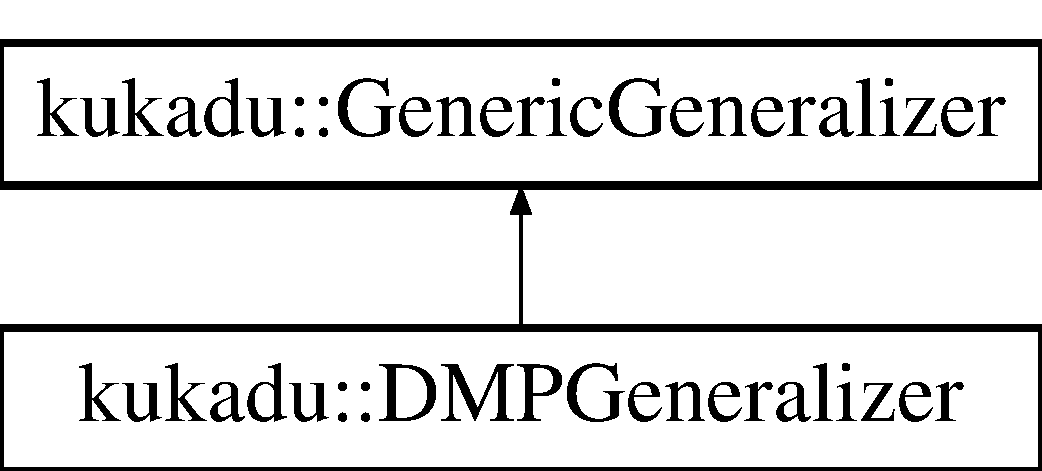
\includegraphics[height=2.000000cm]{classkukadu_1_1DMPGeneralizer}
\end{center}
\end{figure}
\subsection*{Public Member Functions}
\begin{DoxyCompactItemize}
\item 
\hyperlink{classkukadu_1_1DMPGeneralizer_a75bfc264da4632ef2ce2454759b53d9c}{D\-M\-P\-Generalizer} (std\-::string base\-Folder, int deg\-Of\-Freedom, std\-::vector$<$ double $>$ tmpmys, std\-::vector$<$ double $>$ tmpsigmas, double az, double bz)
\begin{DoxyCompactList}\small\item\em constructor \end{DoxyCompactList}\item 
\hypertarget{classkukadu_1_1DMPGeneralizer_a66ae70315e509c84bb1763825a15b2ea}{int \hyperlink{classkukadu_1_1DMPGeneralizer_a66ae70315e509c84bb1763825a15b2ea}{get\-Query\-Point\-Count} ()}\label{classkukadu_1_1DMPGeneralizer_a66ae70315e509c84bb1763825a15b2ea}

\begin{DoxyCompactList}\small\item\em returns number of trajectory samples \end{DoxyCompactList}\item 
\hypertarget{classkukadu_1_1DMPGeneralizer_a603d560be6c932e1715d74bc581900fa}{double {\bfseries get\-Deg\-Of\-Freedom} ()}\label{classkukadu_1_1DMPGeneralizer_a603d560be6c932e1715d74bc581900fa}

\item 
\hyperlink{classkukadu_1_1QueryPoint}{Query\-Point} \hyperlink{classkukadu_1_1DMPGeneralizer_a670a0b673aee54cc4c10f308b1d211a2}{get\-Query\-Point\-By\-Index} (int index)
\begin{DoxyCompactList}\small\item\em returns a sample point by index \end{DoxyCompactList}\item 
K\-U\-K\-A\-D\-U\-\_\-\-S\-H\-A\-R\-E\-D\-\_\-\-P\-T\-R$<$ \hyperlink{classkukadu_1_1JointDmp}{Joint\-Dmp} $>$ \hyperlink{classkukadu_1_1DMPGeneralizer_acb8a703ee5bb8492d2035120ab51942b}{generalize\-Dmp} (\hyperlink{classkukadu_1_1GenericKernel}{Generic\-Kernel} $\ast$trajectory\-Kernel, \hyperlink{classkukadu_1_1GenericKernel}{Generic\-Kernel} $\ast$parameter\-Kernel, arma\-::vec query, double beta)
\begin{DoxyCompactList}\small\item\em returns the generalized trajectory at a certain query point \end{DoxyCompactList}\end{DoxyCompactItemize}


\subsection{Detailed Description}
This class is able to generalize task specific trajectories from previous examples. 

This method works well on tasks, where the sample trajectories are similar in shape. Therefore, several simple trajectories have to be measured and stored in files. 

\subsection{Constructor \& Destructor Documentation}
\hypertarget{classkukadu_1_1DMPGeneralizer_a75bfc264da4632ef2ce2454759b53d9c}{\index{kukadu\-::\-D\-M\-P\-Generalizer@{kukadu\-::\-D\-M\-P\-Generalizer}!D\-M\-P\-Generalizer@{D\-M\-P\-Generalizer}}
\index{D\-M\-P\-Generalizer@{D\-M\-P\-Generalizer}!kukadu::DMPGeneralizer@{kukadu\-::\-D\-M\-P\-Generalizer}}
\subsubsection[{D\-M\-P\-Generalizer}]{\setlength{\rightskip}{0pt plus 5cm}kukadu\-::\-D\-M\-P\-Generalizer\-::\-D\-M\-P\-Generalizer (
\begin{DoxyParamCaption}
\item[{std\-::string}]{base\-Folder, }
\item[{int}]{deg\-Of\-Freedom, }
\item[{std\-::vector$<$ double $>$}]{tmpmys, }
\item[{std\-::vector$<$ double $>$}]{tmpsigmas, }
\item[{double}]{az, }
\item[{double}]{bz}
\end{DoxyParamCaption}
)}}\label{classkukadu_1_1DMPGeneralizer_a75bfc264da4632ef2ce2454759b53d9c}


constructor 


\begin{DoxyParams}{Parameters}
{\em base\-Folder} & folder that contains the sample trajectory files \\
\hline
{\em deg\-Of\-Freedom} & number of degrees of freedom \\
\hline
{\em tmpmys} & defines basis functions for dynamic movement primitives \\
\hline
{\em tmpsigmas} & defines basis functions for dynamic movement primitives \\
\hline
{\em az} & dmp az parameter \\
\hline
{\em bz} & dmp bz parameter \\
\hline
\end{DoxyParams}


\subsection{Member Function Documentation}
\hypertarget{classkukadu_1_1DMPGeneralizer_acb8a703ee5bb8492d2035120ab51942b}{\index{kukadu\-::\-D\-M\-P\-Generalizer@{kukadu\-::\-D\-M\-P\-Generalizer}!generalize\-Dmp@{generalize\-Dmp}}
\index{generalize\-Dmp@{generalize\-Dmp}!kukadu::DMPGeneralizer@{kukadu\-::\-D\-M\-P\-Generalizer}}
\subsubsection[{generalize\-Dmp}]{\setlength{\rightskip}{0pt plus 5cm}K\-U\-K\-A\-D\-U\-\_\-\-S\-H\-A\-R\-E\-D\-\_\-\-P\-T\-R$<$ {\bf Joint\-Dmp} $>$ kukadu\-::\-D\-M\-P\-Generalizer\-::generalize\-Dmp (
\begin{DoxyParamCaption}
\item[{{\bf Generic\-Kernel} $\ast$}]{trajectory\-Kernel, }
\item[{{\bf Generic\-Kernel} $\ast$}]{parameter\-Kernel, }
\item[{arma\-::vec}]{query, }
\item[{double}]{beta}
\end{DoxyParamCaption}
)\hspace{0.3cm}{\ttfamily [virtual]}}}\label{classkukadu_1_1DMPGeneralizer_acb8a703ee5bb8492d2035120ab51942b}


returns the generalized trajectory at a certain query point 


\begin{DoxyParams}{Parameters}
{\em trajectory\-Kernel} & kernel for trajectory shape generalization \\
\hline
{\em parameter\-Kernel} & kernel for trajectory goal generalization \\
\hline
{\em query} & required query point \\
\hline
{\em beta} & beta for Gaussian processes \\
\hline
\end{DoxyParams}


Implements \hyperlink{classkukadu_1_1GenericGeneralizer}{kukadu\-::\-Generic\-Generalizer}.

\hypertarget{classkukadu_1_1DMPGeneralizer_a670a0b673aee54cc4c10f308b1d211a2}{\index{kukadu\-::\-D\-M\-P\-Generalizer@{kukadu\-::\-D\-M\-P\-Generalizer}!get\-Query\-Point\-By\-Index@{get\-Query\-Point\-By\-Index}}
\index{get\-Query\-Point\-By\-Index@{get\-Query\-Point\-By\-Index}!kukadu::DMPGeneralizer@{kukadu\-::\-D\-M\-P\-Generalizer}}
\subsubsection[{get\-Query\-Point\-By\-Index}]{\setlength{\rightskip}{0pt plus 5cm}{\bf Query\-Point} kukadu\-::\-D\-M\-P\-Generalizer\-::get\-Query\-Point\-By\-Index (
\begin{DoxyParamCaption}
\item[{int}]{index}
\end{DoxyParamCaption}
)}}\label{classkukadu_1_1DMPGeneralizer_a670a0b673aee54cc4c10f308b1d211a2}


returns a sample point by index 


\begin{DoxyParams}{Parameters}
{\em index} & index of sample point \\
\hline
\end{DoxyParams}


The documentation for this class was generated from the following files\-:\begin{DoxyCompactItemize}
\item 
/home/c7031109/iis\-\_\-robot\-\_\-sw/iis\-\_\-catkin\-\_\-ws/src/kukadu/include/kukadu/control/dmpgeneralizer.\-hpp\item 
/home/c7031109/iis\-\_\-robot\-\_\-sw/iis\-\_\-catkin\-\_\-ws/src/kukadu/src/control/dmpgeneralizer.\-cpp\end{DoxyCompactItemize}

\hypertarget{classkukadu_1_1DMPReinforcer}{\section{kukadu\-:\-:D\-M\-P\-Reinforcer Class Reference}
\label{classkukadu_1_1DMPReinforcer}\index{kukadu\-::\-D\-M\-P\-Reinforcer@{kukadu\-::\-D\-M\-P\-Reinforcer}}
}


The \hyperlink{classkukadu_1_1DMPReinforcer}{D\-M\-P\-Reinforcer} provides a general framework for reinforcement learning.  




{\ttfamily \#include $<$dmpreinforcer.\-hpp$>$}

\subsection*{Public Member Functions}
\begin{DoxyCompactItemize}
\item 
\hyperlink{classkukadu_1_1DMPReinforcer_af7601db62c48a9afd1918996a1cea1a7}{D\-M\-P\-Reinforcer} (\hyperlink{classkukadu_1_1CostComputer}{Cost\-Computer} $\ast$cost, K\-U\-K\-A\-D\-U\-\_\-\-S\-H\-A\-R\-E\-D\-\_\-\-P\-T\-R$<$ \hyperlink{classkukadu_1_1ControlQueue}{Control\-Queue} $>$ movement\-Queue, double ac, double tol\-Abs\-Err, double tol\-Rel\-Err)
\begin{DoxyCompactList}\small\item\em constructor \end{DoxyCompactList}\item 
\hypertarget{classkukadu_1_1DMPReinforcer_a759bd3c0954e4287f8166a4115fd2c55}{void {\bfseries set\-Last\-Update} (K\-U\-K\-A\-D\-U\-\_\-\-S\-H\-A\-R\-E\-D\-\_\-\-P\-T\-R$<$ \hyperlink{classkukadu_1_1Dmp}{Dmp} $>$ last\-Update)}\label{classkukadu_1_1DMPReinforcer_a759bd3c0954e4287f8166a4115fd2c55}

\item 
void \hyperlink{classkukadu_1_1DMPReinforcer_ab2597f0265192981ab70cadc9fa35a05}{perform\-Rollout} (int do\-Simulation, int do\-Execution)
\begin{DoxyCompactList}\small\item\em executes rollout. first, the trajectory is simulated and the user is asked, whether the trajectory really should be executed \end{DoxyCompactList}\item 
\hypertarget{classkukadu_1_1DMPReinforcer_ab9ba3dc996de2223db6fb8d0dd79c429}{bool \hyperlink{classkukadu_1_1DMPReinforcer_ab9ba3dc996de2223db6fb8d0dd79c429}{get\-Is\-First\-Iteration} ()}\label{classkukadu_1_1DMPReinforcer_ab9ba3dc996de2223db6fb8d0dd79c429}

\begin{DoxyCompactList}\small\item\em returns true if the first iteration has not been performed yet \end{DoxyCompactList}\item 
\hypertarget{classkukadu_1_1DMPReinforcer_a9b75bfd5aefec6e93dd6ac6a130da023}{double \hyperlink{classkukadu_1_1DMPReinforcer_a9b75bfd5aefec6e93dd6ac6a130da023}{get\-Tol\-Abs\-Err} ()}\label{classkukadu_1_1DMPReinforcer_a9b75bfd5aefec6e93dd6ac6a130da023}

\begin{DoxyCompactList}\small\item\em returns simulation tolerated absolute error \end{DoxyCompactList}\item 
\hypertarget{classkukadu_1_1DMPReinforcer_a377d0dc8df73872a2d4c10e8247b0862}{double \hyperlink{classkukadu_1_1DMPReinforcer_a377d0dc8df73872a2d4c10e8247b0862}{get\-Tol\-Rel\-Err} ()}\label{classkukadu_1_1DMPReinforcer_a377d0dc8df73872a2d4c10e8247b0862}

\begin{DoxyCompactList}\small\item\em returns simulation tolerated relative error \end{DoxyCompactList}\item 
\hypertarget{classkukadu_1_1DMPReinforcer_abab6e2bd6abdd613335ecc7186e3d89c}{K\-U\-K\-A\-D\-U\-\_\-\-S\-H\-A\-R\-E\-D\-\_\-\-P\-T\-R$<$ \hyperlink{classkukadu_1_1Dmp}{Dmp} $>$ {\bfseries get\-Last\-Update} ()}\label{classkukadu_1_1DMPReinforcer_abab6e2bd6abdd613335ecc7186e3d89c}

\item 
\hypertarget{classkukadu_1_1DMPReinforcer_aa8722bbe4c69ca344c82a2e5aaa85d74}{K\-U\-K\-A\-D\-U\-\_\-\-S\-H\-A\-R\-E\-D\-\_\-\-P\-T\-R\\*
$<$ \hyperlink{classkukadu_1_1ControllerResult}{Controller\-Result} $>$ {\bfseries get\-Last\-Update\-Res} ()}\label{classkukadu_1_1DMPReinforcer_aa8722bbe4c69ca344c82a2e5aaa85d74}

\item 
\hypertarget{classkukadu_1_1DMPReinforcer_af88dad66482a357f0c4bcfc94aeac631}{virtual K\-U\-K\-A\-D\-U\-\_\-\-S\-H\-A\-R\-E\-D\-\_\-\-P\-T\-R$<$ \hyperlink{classkukadu_1_1Dmp}{Dmp} $>$ {\bfseries update\-Step} ()=0}\label{classkukadu_1_1DMPReinforcer_af88dad66482a357f0c4bcfc94aeac631}

\item 
\hypertarget{classkukadu_1_1DMPReinforcer_ad4032a5137fd6ff47b09455361e2ebe3}{std\-::vector$<$ K\-U\-K\-A\-D\-U\-\_\-\-S\-H\-A\-R\-E\-D\-\_\-\-P\-T\-R\\*
$<$ \hyperlink{classkukadu_1_1Dmp}{Dmp} $>$ $>$ {\bfseries get\-Last\-Rollout\-Parameters} ()}\label{classkukadu_1_1DMPReinforcer_ad4032a5137fd6ff47b09455361e2ebe3}

\item 
\hypertarget{classkukadu_1_1DMPReinforcer_a32bac8a17c007d40673b05f34ee017ca}{virtual std\-::vector\\*
$<$ K\-U\-K\-A\-D\-U\-\_\-\-S\-H\-A\-R\-E\-D\-\_\-\-P\-T\-R$<$ \hyperlink{classkukadu_1_1Dmp}{Dmp} $>$ $>$ \hyperlink{classkukadu_1_1DMPReinforcer_a32bac8a17c007d40673b05f34ee017ca}{get\-Initial\-Rollout} ()=0}\label{classkukadu_1_1DMPReinforcer_a32bac8a17c007d40673b05f34ee017ca}

\begin{DoxyCompactList}\small\item\em returns the first rollout of the reinforcement learning algorithm \end{DoxyCompactList}\item 
\hypertarget{classkukadu_1_1DMPReinforcer_abf1b944f57802f5ea3470be9746ad5ab}{virtual std\-::vector\\*
$<$ K\-U\-K\-A\-D\-U\-\_\-\-S\-H\-A\-R\-E\-D\-\_\-\-P\-T\-R$<$ \hyperlink{classkukadu_1_1Dmp}{Dmp} $>$ $>$ \hyperlink{classkukadu_1_1DMPReinforcer_abf1b944f57802f5ea3470be9746ad5ab}{compute\-Rollout\-Paramters} ()=0}\label{classkukadu_1_1DMPReinforcer_abf1b944f57802f5ea3470be9746ad5ab}

\begin{DoxyCompactList}\small\item\em computes the dmp parameters for the next rollout \end{DoxyCompactList}\item 
\hypertarget{classkukadu_1_1DMPReinforcer_ae1e7b4f023979e5076897102a54066c3}{std\-::vector$<$ double $>$ \hyperlink{classkukadu_1_1DMPReinforcer_ae1e7b4f023979e5076897102a54066c3}{get\-Last\-Rollout\-Cost} ()}\label{classkukadu_1_1DMPReinforcer_ae1e7b4f023979e5076897102a54066c3}

\begin{DoxyCompactList}\small\item\em returns cost for the last executed rollout \end{DoxyCompactList}\item 
\hypertarget{classkukadu_1_1DMPReinforcer_a53f28e972c75ec336d55aee227ba5b30}{std\-::vector$<$ K\-U\-K\-A\-D\-U\-\_\-\-S\-H\-A\-R\-E\-D\-\_\-\-P\-T\-R\\*
$<$ \hyperlink{classkukadu_1_1ControllerResult}{Controller\-Result} $>$ $>$ {\bfseries get\-Last\-Execution\-Results} ()}\label{classkukadu_1_1DMPReinforcer_a53f28e972c75ec336d55aee227ba5b30}

\end{DoxyCompactItemize}


\subsection{Detailed Description}
The \hyperlink{classkukadu_1_1DMPReinforcer}{D\-M\-P\-Reinforcer} provides a general framework for reinforcement learning. 

It is an abstract class that implements elementary functionality that should be in common for all reinforcement learning methods (such as rollout execution). A concrete implementation of the \hyperlink{classkukadu_1_1DMPReinforcer}{D\-M\-P\-Reinforcer} has to implement the missing parts such as the methods get\-Initial\-Rollout and compute\-Rollout\-Paramters. 

\subsection{Constructor \& Destructor Documentation}
\hypertarget{classkukadu_1_1DMPReinforcer_af7601db62c48a9afd1918996a1cea1a7}{\index{kukadu\-::\-D\-M\-P\-Reinforcer@{kukadu\-::\-D\-M\-P\-Reinforcer}!D\-M\-P\-Reinforcer@{D\-M\-P\-Reinforcer}}
\index{D\-M\-P\-Reinforcer@{D\-M\-P\-Reinforcer}!kukadu::DMPReinforcer@{kukadu\-::\-D\-M\-P\-Reinforcer}}
\subsubsection[{D\-M\-P\-Reinforcer}]{\setlength{\rightskip}{0pt plus 5cm}kukadu\-::\-D\-M\-P\-Reinforcer\-::\-D\-M\-P\-Reinforcer (
\begin{DoxyParamCaption}
\item[{{\bf Cost\-Computer} $\ast$}]{cost, }
\item[{K\-U\-K\-A\-D\-U\-\_\-\-S\-H\-A\-R\-E\-D\-\_\-\-P\-T\-R$<$ {\bf Control\-Queue} $>$}]{movement\-Queue, }
\item[{double}]{ac, }
\item[{double}]{tol\-Abs\-Err, }
\item[{double}]{tol\-Rel\-Err}
\end{DoxyParamCaption}
)}}\label{classkukadu_1_1DMPReinforcer_af7601db62c48a9afd1918996a1cea1a7}


constructor 


\begin{DoxyParams}{Parameters}
{\em cost} & \hyperlink{classkukadu_1_1CostComputer}{Cost\-Computer} instance that computes the cost of a given rollout \\
\hline
{\em movement\-Queue} & \hyperlink{classkukadu_1_1ControlQueue}{Control\-Queue} instance for robot execution \\
\hline
{\em ac} & dmp phase stopping parameter \\
\hline
{\em dmp\-Step\-Size} & step size for dmp execution \\
\hline
{\em tol\-Abs\-Err} & absolute tolerated error for numerical approximation \\
\hline
{\em tol\-Rel\-Err} & relative tolerated error for numerical approximation \\
\hline
\end{DoxyParams}


\subsection{Member Function Documentation}
\hypertarget{classkukadu_1_1DMPReinforcer_ab2597f0265192981ab70cadc9fa35a05}{\index{kukadu\-::\-D\-M\-P\-Reinforcer@{kukadu\-::\-D\-M\-P\-Reinforcer}!perform\-Rollout@{perform\-Rollout}}
\index{perform\-Rollout@{perform\-Rollout}!kukadu::DMPReinforcer@{kukadu\-::\-D\-M\-P\-Reinforcer}}
\subsubsection[{perform\-Rollout}]{\setlength{\rightskip}{0pt plus 5cm}void kukadu\-::\-D\-M\-P\-Reinforcer\-::perform\-Rollout (
\begin{DoxyParamCaption}
\item[{int}]{do\-Simulation, }
\item[{int}]{do\-Execution}
\end{DoxyParamCaption}
)}}\label{classkukadu_1_1DMPReinforcer_ab2597f0265192981ab70cadc9fa35a05}


executes rollout. first, the trajectory is simulated and the user is asked, whether the trajectory really should be executed 


\begin{DoxyParams}{Parameters}
{\em do\-Simulation} & flag whether trajectory should be simulated \\
\hline
{\em do\-Execution} & flag whether trajectory should be executed at robot \\
\hline
\end{DoxyParams}


The documentation for this class was generated from the following files\-:\begin{DoxyCompactItemize}
\item 
/home/c7031109/iis\-\_\-robot\-\_\-sw/iis\-\_\-catkin\-\_\-ws/src/kukadu/include/kukadu/learning/rl/dmpreinforcer.\-hpp\item 
/home/c7031109/iis\-\_\-robot\-\_\-sw/iis\-\_\-catkin\-\_\-ws/src/kukadu/src/learning/reinforcement\-\_\-learning/dmpreinforcer.\-cpp\end{DoxyCompactItemize}

\hypertarget{classkukadu_1_1DmpRewardComputer}{\section{kukadu\-:\-:Dmp\-Reward\-Computer Class Reference}
\label{classkukadu_1_1DmpRewardComputer}\index{kukadu\-::\-Dmp\-Reward\-Computer@{kukadu\-::\-Dmp\-Reward\-Computer}}
}
Inheritance diagram for kukadu\-:\-:Dmp\-Reward\-Computer\-:\begin{figure}[H]
\begin{center}
\leavevmode
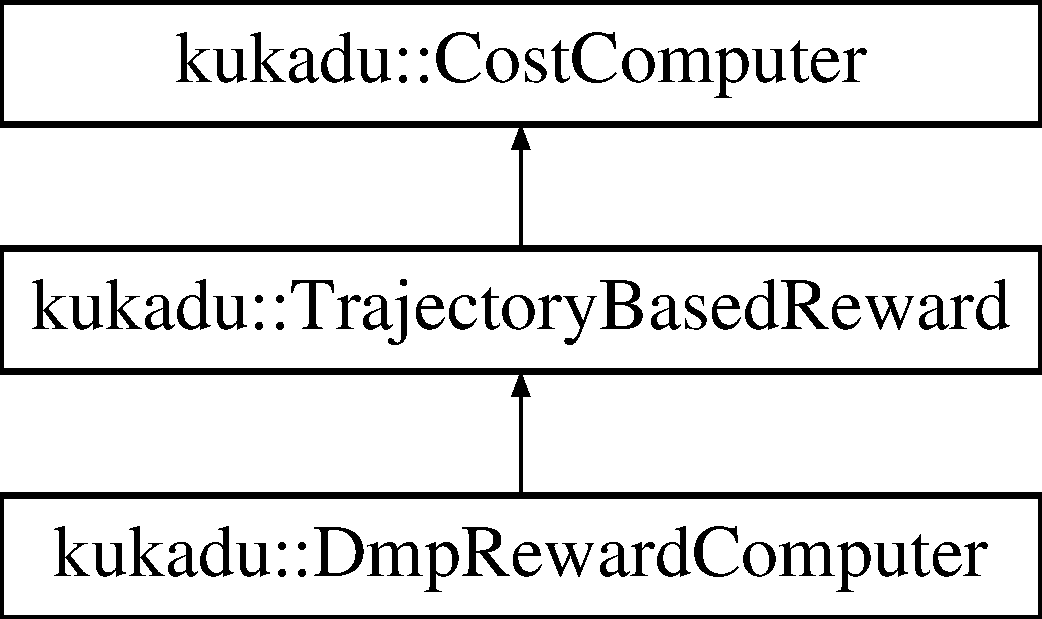
\includegraphics[height=3.000000cm]{classkukadu_1_1DmpRewardComputer}
\end{center}
\end{figure}
\subsection*{Public Member Functions}
\begin{DoxyCompactItemize}
\item 
\hypertarget{classkukadu_1_1DmpRewardComputer_ac7250816fcccadabc1cab8a8ea051651}{{\bfseries Dmp\-Reward\-Computer} (std\-::string file, double az, double bz, double time\-Step, int deg\-Of\-Freedom, double tmax, double step)}\label{classkukadu_1_1DmpRewardComputer_ac7250816fcccadabc1cab8a8ea051651}

\item 
\hypertarget{classkukadu_1_1DmpRewardComputer_aef2a5a9a1703bd183e09eac8becba726}{arma\-::vec {\bfseries compute\-Fun} (double t)}\label{classkukadu_1_1DmpRewardComputer_aef2a5a9a1703bd183e09eac8becba726}

\end{DoxyCompactItemize}


The documentation for this class was generated from the following files\-:\begin{DoxyCompactItemize}
\item 
/home/c7031109/iis\-\_\-robot\-\_\-sw/iis\-\_\-catkin\-\_\-ws/src/kukadu/include/kukadu/learning/rl/dmprewardcomputer.\-hpp\item 
/home/c7031109/iis\-\_\-robot\-\_\-sw/iis\-\_\-catkin\-\_\-ws/src/kukadu/src/learning/reinforcement\-\_\-learning/dmprewardcomputer.\-cpp\end{DoxyCompactItemize}

\hypertarget{classkukadu_1_1DMPTrajectoryGenerator}{\section{kukadu\-:\-:D\-M\-P\-Trajectory\-Generator Class Reference}
\label{classkukadu_1_1DMPTrajectoryGenerator}\index{kukadu\-::\-D\-M\-P\-Trajectory\-Generator@{kukadu\-::\-D\-M\-P\-Trajectory\-Generator}}
}


Implements the \hyperlink{classkukadu_1_1TrajectoryGenerator}{Trajectory\-Generator} interface for dynamic movement primitives.  




{\ttfamily \#include $<$dmptrajectorygenerator.\-hpp$>$}

Inheritance diagram for kukadu\-:\-:D\-M\-P\-Trajectory\-Generator\-:\begin{figure}[H]
\begin{center}
\leavevmode
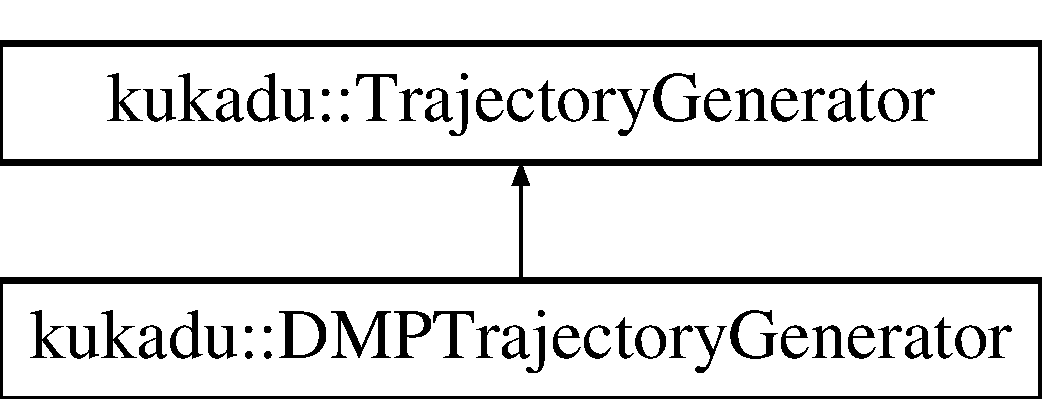
\includegraphics[height=2.000000cm]{classkukadu_1_1DMPTrajectoryGenerator}
\end{center}
\end{figure}
\subsection*{Public Member Functions}
\begin{DoxyCompactItemize}
\item 
\hyperlink{classkukadu_1_1DMPTrajectoryGenerator_a0bf8fd4b7bc9aded7f0929743228e73a}{D\-M\-P\-Trajectory\-Generator} (std\-::vector$<$ \hyperlink{classkukadu_1_1DMPBase}{D\-M\-P\-Base} $>$ base\-Def, double ax, double tau)
\begin{DoxyCompactList}\small\item\em constructor \end{DoxyCompactList}\item 
double \hyperlink{classkukadu_1_1DMPTrajectoryGenerator_a6072064f086581981d1b1540953d4bd0}{evaluate\-Basis\-Function} (double x, int fun)
\begin{DoxyCompactList}\small\item\em evaluates the value of a single basis function \end{DoxyCompactList}\item 
double \hyperlink{classkukadu_1_1DMPTrajectoryGenerator_ad85bfa03fb1b426b9c808607a22d4f95}{evaluate\-Basis\-Function\-Non\-Exponential} (double x, int fun)
\begin{DoxyCompactList}\small\item\em computes the basis function value by setting x = e$^\wedge$(-\/ax / tau $\ast$ x) \end{DoxyCompactList}\item 
double \hyperlink{classkukadu_1_1DMPTrajectoryGenerator_aa14fb2c9ba08e0a8323090593b46d7f4}{evaluate\-By\-Coefficients\-Single} (double x, arma\-::vec coeff)
\begin{DoxyCompactList}\small\item\em evaluates the linear combination of basis functions by defining the coefficients for a single value x \end{DoxyCompactList}\item 
double \hyperlink{classkukadu_1_1DMPTrajectoryGenerator_a48f050d0bded75b1babaafda54aa0432}{evaluate\-By\-Coefficients\-Single\-Non\-Exponential} (double x, arma\-::vec coeff)
\begin{DoxyCompactList}\small\item\em computes the linear combination of basis functions values by setting x = e$^\wedge$(-\/ax / tau $\ast$ x) \end{DoxyCompactList}\item 
arma\-::vec \hyperlink{classkukadu_1_1DMPTrajectoryGenerator_affb281e54fbddd566338d3c8e826bd40}{evaluate\-By\-Coefficients\-Multiple} (arma\-::vec x, int sample\-Count, arma\-::vec coeff)
\begin{DoxyCompactList}\small\item\em performs the same as evaluate\-By\-Coefficients\-Single, but for multiple values of x \end{DoxyCompactList}\item 
arma\-::vec \hyperlink{classkukadu_1_1DMPTrajectoryGenerator_a759b1a5b259bcc7ab26554232f94a393}{evaluate\-By\-Coefficients\-Multiple\-Non\-Exponential} (arma\-::vec x, int sample\-Count, arma\-::vec coeff)
\begin{DoxyCompactList}\small\item\em computes the linear combination of basis functions values for multiple positions by setting x = e$^\wedge$(-\/ax / tau $\ast$ x) \end{DoxyCompactList}\item 
\hypertarget{classkukadu_1_1DMPTrajectoryGenerator_a2554959c04ce802829324fced3bb872b}{int \hyperlink{classkukadu_1_1DMPTrajectoryGenerator_a2554959c04ce802829324fced3bb872b}{get\-Basis\-Function\-Count} ()}\label{classkukadu_1_1DMPTrajectoryGenerator_a2554959c04ce802829324fced3bb872b}

\begin{DoxyCompactList}\small\item\em returns the number of basis functions \end{DoxyCompactList}\item 
\hypertarget{classkukadu_1_1DMPTrajectoryGenerator_a9b6535bbc5e82c84238ebe41f04bca3f}{std\-::string \hyperlink{classkukadu_1_1DMPTrajectoryGenerator_a9b6535bbc5e82c84238ebe41f04bca3f}{get\-Trajectory\-Type} ()}\label{classkukadu_1_1DMPTrajectoryGenerator_a9b6535bbc5e82c84238ebe41f04bca3f}

\begin{DoxyCompactList}\small\item\em returns the name of the basis function system as a string \end{DoxyCompactList}\end{DoxyCompactItemize}


\subsection{Detailed Description}
Implements the \hyperlink{classkukadu_1_1TrajectoryGenerator}{Trajectory\-Generator} interface for dynamic movement primitives. 

This class provides the basis functions for learning dynamic movement primitives with linear regression (see papers on dmps) 

\subsection{Constructor \& Destructor Documentation}
\hypertarget{classkukadu_1_1DMPTrajectoryGenerator_a0bf8fd4b7bc9aded7f0929743228e73a}{\index{kukadu\-::\-D\-M\-P\-Trajectory\-Generator@{kukadu\-::\-D\-M\-P\-Trajectory\-Generator}!D\-M\-P\-Trajectory\-Generator@{D\-M\-P\-Trajectory\-Generator}}
\index{D\-M\-P\-Trajectory\-Generator@{D\-M\-P\-Trajectory\-Generator}!kukadu::DMPTrajectoryGenerator@{kukadu\-::\-D\-M\-P\-Trajectory\-Generator}}
\subsubsection[{D\-M\-P\-Trajectory\-Generator}]{\setlength{\rightskip}{0pt plus 5cm}kukadu\-::\-D\-M\-P\-Trajectory\-Generator\-::\-D\-M\-P\-Trajectory\-Generator (
\begin{DoxyParamCaption}
\item[{std\-::vector$<$ {\bf D\-M\-P\-Base} $>$}]{base\-Def, }
\item[{double}]{ax, }
\item[{double}]{tau}
\end{DoxyParamCaption}
)}}\label{classkukadu_1_1DMPTrajectoryGenerator_a0bf8fd4b7bc9aded7f0929743228e73a}


constructor 


\begin{DoxyParams}{Parameters}
{\em base\-Def} & defines the basis functions by setting the means and variances of the Gaussian basis functions \\
\hline
{\em ax} & dmp constant \\
\hline
{\em tau} & dmp time constant \\
\hline
\end{DoxyParams}


\subsection{Member Function Documentation}
\hypertarget{classkukadu_1_1DMPTrajectoryGenerator_a6072064f086581981d1b1540953d4bd0}{\index{kukadu\-::\-D\-M\-P\-Trajectory\-Generator@{kukadu\-::\-D\-M\-P\-Trajectory\-Generator}!evaluate\-Basis\-Function@{evaluate\-Basis\-Function}}
\index{evaluate\-Basis\-Function@{evaluate\-Basis\-Function}!kukadu::DMPTrajectoryGenerator@{kukadu\-::\-D\-M\-P\-Trajectory\-Generator}}
\subsubsection[{evaluate\-Basis\-Function}]{\setlength{\rightskip}{0pt plus 5cm}double kukadu\-::\-D\-M\-P\-Trajectory\-Generator\-::evaluate\-Basis\-Function (
\begin{DoxyParamCaption}
\item[{double}]{x, }
\item[{int}]{fun}
\end{DoxyParamCaption}
)\hspace{0.3cm}{\ttfamily [virtual]}}}\label{classkukadu_1_1DMPTrajectoryGenerator_a6072064f086581981d1b1540953d4bd0}


evaluates the value of a single basis function 


\begin{DoxyParams}{Parameters}
{\em x} & value, where the basis function should be evaluated \\
\hline
{\em fun} & basis function index that specifies the basis function \\
\hline
\end{DoxyParams}


Implements \hyperlink{classkukadu_1_1TrajectoryGenerator_abbd50214ceb85171e7103a1fded7fd91}{kukadu\-::\-Trajectory\-Generator}.

\hypertarget{classkukadu_1_1DMPTrajectoryGenerator_ad85bfa03fb1b426b9c808607a22d4f95}{\index{kukadu\-::\-D\-M\-P\-Trajectory\-Generator@{kukadu\-::\-D\-M\-P\-Trajectory\-Generator}!evaluate\-Basis\-Function\-Non\-Exponential@{evaluate\-Basis\-Function\-Non\-Exponential}}
\index{evaluate\-Basis\-Function\-Non\-Exponential@{evaluate\-Basis\-Function\-Non\-Exponential}!kukadu::DMPTrajectoryGenerator@{kukadu\-::\-D\-M\-P\-Trajectory\-Generator}}
\subsubsection[{evaluate\-Basis\-Function\-Non\-Exponential}]{\setlength{\rightskip}{0pt plus 5cm}double kukadu\-::\-D\-M\-P\-Trajectory\-Generator\-::evaluate\-Basis\-Function\-Non\-Exponential (
\begin{DoxyParamCaption}
\item[{double}]{x, }
\item[{int}]{fun}
\end{DoxyParamCaption}
)}}\label{classkukadu_1_1DMPTrajectoryGenerator_ad85bfa03fb1b426b9c808607a22d4f95}


computes the basis function value by setting x = e$^\wedge$(-\/ax / tau $\ast$ x) 


\begin{DoxyParams}{Parameters}
{\em x} & position to evaluate \\
\hline
{\em fun} & basis function index \\
\hline
\end{DoxyParams}
\hypertarget{classkukadu_1_1DMPTrajectoryGenerator_affb281e54fbddd566338d3c8e826bd40}{\index{kukadu\-::\-D\-M\-P\-Trajectory\-Generator@{kukadu\-::\-D\-M\-P\-Trajectory\-Generator}!evaluate\-By\-Coefficients\-Multiple@{evaluate\-By\-Coefficients\-Multiple}}
\index{evaluate\-By\-Coefficients\-Multiple@{evaluate\-By\-Coefficients\-Multiple}!kukadu::DMPTrajectoryGenerator@{kukadu\-::\-D\-M\-P\-Trajectory\-Generator}}
\subsubsection[{evaluate\-By\-Coefficients\-Multiple}]{\setlength{\rightskip}{0pt plus 5cm}vec kukadu\-::\-D\-M\-P\-Trajectory\-Generator\-::evaluate\-By\-Coefficients\-Multiple (
\begin{DoxyParamCaption}
\item[{arma\-::vec}]{x, }
\item[{int}]{sample\-Count, }
\item[{arma\-::vec}]{coeff}
\end{DoxyParamCaption}
)\hspace{0.3cm}{\ttfamily [virtual]}}}\label{classkukadu_1_1DMPTrajectoryGenerator_affb281e54fbddd566338d3c8e826bd40}


performs the same as evaluate\-By\-Coefficients\-Single, but for multiple values of x 


\begin{DoxyParams}{Parameters}
{\em x} & vector of evaluation points \\
\hline
{\em sample\-Count} & size of vector x \\
\hline
{\em coeff} & coefficients that have to be used for computing the linear combination \\
\hline
\end{DoxyParams}


Implements \hyperlink{classkukadu_1_1TrajectoryGenerator_a80e470d557ac5fc9a075b582d97bf67b}{kukadu\-::\-Trajectory\-Generator}.

\hypertarget{classkukadu_1_1DMPTrajectoryGenerator_a759b1a5b259bcc7ab26554232f94a393}{\index{kukadu\-::\-D\-M\-P\-Trajectory\-Generator@{kukadu\-::\-D\-M\-P\-Trajectory\-Generator}!evaluate\-By\-Coefficients\-Multiple\-Non\-Exponential@{evaluate\-By\-Coefficients\-Multiple\-Non\-Exponential}}
\index{evaluate\-By\-Coefficients\-Multiple\-Non\-Exponential@{evaluate\-By\-Coefficients\-Multiple\-Non\-Exponential}!kukadu::DMPTrajectoryGenerator@{kukadu\-::\-D\-M\-P\-Trajectory\-Generator}}
\subsubsection[{evaluate\-By\-Coefficients\-Multiple\-Non\-Exponential}]{\setlength{\rightskip}{0pt plus 5cm}vec kukadu\-::\-D\-M\-P\-Trajectory\-Generator\-::evaluate\-By\-Coefficients\-Multiple\-Non\-Exponential (
\begin{DoxyParamCaption}
\item[{arma\-::vec}]{x, }
\item[{int}]{sample\-Count, }
\item[{arma\-::vec}]{coeff}
\end{DoxyParamCaption}
)}}\label{classkukadu_1_1DMPTrajectoryGenerator_a759b1a5b259bcc7ab26554232f94a393}


computes the linear combination of basis functions values for multiple positions by setting x = e$^\wedge$(-\/ax / tau $\ast$ x) 


\begin{DoxyParams}{Parameters}
{\em x} & vector of positions to evaluate \\
\hline
{\em sample\-Count} & size of vector x \\
\hline
{\em coeff} & vector of basis function coefficients \\
\hline
\end{DoxyParams}
\hypertarget{classkukadu_1_1DMPTrajectoryGenerator_aa14fb2c9ba08e0a8323090593b46d7f4}{\index{kukadu\-::\-D\-M\-P\-Trajectory\-Generator@{kukadu\-::\-D\-M\-P\-Trajectory\-Generator}!evaluate\-By\-Coefficients\-Single@{evaluate\-By\-Coefficients\-Single}}
\index{evaluate\-By\-Coefficients\-Single@{evaluate\-By\-Coefficients\-Single}!kukadu::DMPTrajectoryGenerator@{kukadu\-::\-D\-M\-P\-Trajectory\-Generator}}
\subsubsection[{evaluate\-By\-Coefficients\-Single}]{\setlength{\rightskip}{0pt plus 5cm}double kukadu\-::\-D\-M\-P\-Trajectory\-Generator\-::evaluate\-By\-Coefficients\-Single (
\begin{DoxyParamCaption}
\item[{double}]{x, }
\item[{arma\-::vec}]{coeff}
\end{DoxyParamCaption}
)\hspace{0.3cm}{\ttfamily [virtual]}}}\label{classkukadu_1_1DMPTrajectoryGenerator_aa14fb2c9ba08e0a8323090593b46d7f4}


evaluates the linear combination of basis functions by defining the coefficients for a single value x 


\begin{DoxyParams}{Parameters}
{\em x} & value, where the basis functions should be evaluated \\
\hline
{\em coeff} & coefficients that have to be used for computing the linear combination \\
\hline
\end{DoxyParams}


Implements \hyperlink{classkukadu_1_1TrajectoryGenerator_a3cd7129235c868a1cad3d56f3a05ad49}{kukadu\-::\-Trajectory\-Generator}.

\hypertarget{classkukadu_1_1DMPTrajectoryGenerator_a48f050d0bded75b1babaafda54aa0432}{\index{kukadu\-::\-D\-M\-P\-Trajectory\-Generator@{kukadu\-::\-D\-M\-P\-Trajectory\-Generator}!evaluate\-By\-Coefficients\-Single\-Non\-Exponential@{evaluate\-By\-Coefficients\-Single\-Non\-Exponential}}
\index{evaluate\-By\-Coefficients\-Single\-Non\-Exponential@{evaluate\-By\-Coefficients\-Single\-Non\-Exponential}!kukadu::DMPTrajectoryGenerator@{kukadu\-::\-D\-M\-P\-Trajectory\-Generator}}
\subsubsection[{evaluate\-By\-Coefficients\-Single\-Non\-Exponential}]{\setlength{\rightskip}{0pt plus 5cm}double kukadu\-::\-D\-M\-P\-Trajectory\-Generator\-::evaluate\-By\-Coefficients\-Single\-Non\-Exponential (
\begin{DoxyParamCaption}
\item[{double}]{x, }
\item[{arma\-::vec}]{coeff}
\end{DoxyParamCaption}
)}}\label{classkukadu_1_1DMPTrajectoryGenerator_a48f050d0bded75b1babaafda54aa0432}


computes the linear combination of basis functions values by setting x = e$^\wedge$(-\/ax / tau $\ast$ x) 


\begin{DoxyParams}{Parameters}
{\em x} & position to evaluate \\
\hline
{\em coeff} & vector of basis function coefficients \\
\hline
\end{DoxyParams}


The documentation for this class was generated from the following files\-:\begin{DoxyCompactItemize}
\item 
/home/c7031109/iis\-\_\-robot\-\_\-sw/iis\-\_\-catkin\-\_\-ws/src/kukadu/include/kukadu/control/dmptrajectorygenerator.\-hpp\item 
/home/c7031109/iis\-\_\-robot\-\_\-sw/iis\-\_\-catkin\-\_\-ws/src/kukadu/src/control/dmptrajectorygenerator.\-cpp\end{DoxyCompactItemize}

\hypertarget{classkukadu_1_1EnvironmentReward}{\section{kukadu\-:\-:Environment\-Reward Class Reference}
\label{classkukadu_1_1EnvironmentReward}\index{kukadu\-::\-Environment\-Reward@{kukadu\-::\-Environment\-Reward}}
}
Inheritance diagram for kukadu\-:\-:Environment\-Reward\-:\begin{figure}[H]
\begin{center}
\leavevmode
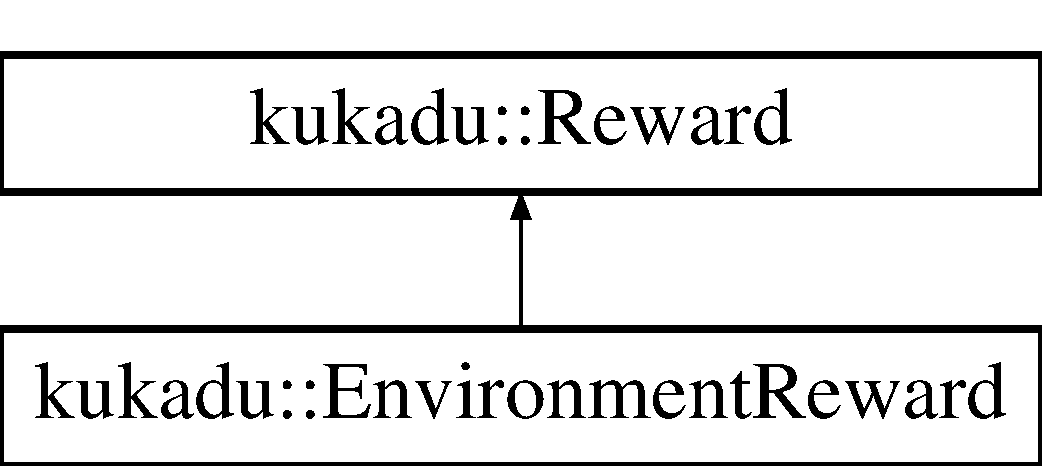
\includegraphics[height=2.000000cm]{classkukadu_1_1EnvironmentReward}
\end{center}
\end{figure}
\subsection*{Public Member Functions}
\begin{DoxyCompactItemize}
\item 
\hypertarget{classkukadu_1_1EnvironmentReward_a9b7aafdf7759916c3424c39e2e3fbded}{{\bfseries Environment\-Reward} (K\-U\-K\-A\-D\-U\-\_\-\-S\-H\-A\-R\-E\-D\-\_\-\-P\-T\-R$<$ kukadu\-\_\-mersenne\-\_\-twister $>$ generator, double std\-Reward)}\label{classkukadu_1_1EnvironmentReward_a9b7aafdf7759916c3424c39e2e3fbded}

\item 
\hypertarget{classkukadu_1_1EnvironmentReward_ab867e2a044297dca24d26ad931a025cc}{virtual int {\bfseries get\-Dimensionality} ()}\label{classkukadu_1_1EnvironmentReward_ab867e2a044297dca24d26ad931a025cc}

\item 
\hypertarget{classkukadu_1_1EnvironmentReward_a1f6effdfb0a9e305b18f021f65cfc61e}{virtual K\-U\-K\-A\-D\-U\-\_\-\-S\-H\-A\-R\-E\-D\-\_\-\-P\-T\-R\\*
$<$ \hyperlink{classkukadu_1_1PerceptClip}{Percept\-Clip} $>$ {\bfseries generate\-Next\-Percept\-Clip} (int immunity)}\label{classkukadu_1_1EnvironmentReward_a1f6effdfb0a9e305b18f021f65cfc61e}

\item 
\hypertarget{classkukadu_1_1EnvironmentReward_ae1d92344047594f9b216c8bf26949985}{virtual K\-U\-K\-A\-D\-U\-\_\-\-S\-H\-A\-R\-E\-D\-\_\-\-P\-T\-R\\*
$<$ std\-::vector\\*
$<$ K\-U\-K\-A\-D\-U\-\_\-\-S\-H\-A\-R\-E\-D\-\_\-\-P\-T\-R\\*
$<$ \hyperlink{classkukadu_1_1ActionClip}{Action\-Clip} $>$ $>$ $>$ {\bfseries generate\-Action\-Clips} ()}\label{classkukadu_1_1EnvironmentReward_ae1d92344047594f9b216c8bf26949985}

\item 
\hypertarget{classkukadu_1_1EnvironmentReward_a5818ba354251ea73759e7c4a89c0fe1a}{virtual K\-U\-K\-A\-D\-U\-\_\-\-S\-H\-A\-R\-E\-D\-\_\-\-P\-T\-R\\*
$<$ std\-::vector\\*
$<$ K\-U\-K\-A\-D\-U\-\_\-\-S\-H\-A\-R\-E\-D\-\_\-\-P\-T\-R\\*
$<$ \hyperlink{classkukadu_1_1PerceptClip}{Percept\-Clip} $>$ $>$ $>$ {\bfseries generate\-Percept\-Clips} ()}\label{classkukadu_1_1EnvironmentReward_a5818ba354251ea73759e7c4a89c0fe1a}

\end{DoxyCompactItemize}
\subsection*{Protected Member Functions}
\begin{DoxyCompactItemize}
\item 
\hypertarget{classkukadu_1_1EnvironmentReward_add69df93b12c6e217570b1b736d959e7}{virtual double {\bfseries compute\-Reward\-Internal} (K\-U\-K\-A\-D\-U\-\_\-\-S\-H\-A\-R\-E\-D\-\_\-\-P\-T\-R$<$ \hyperlink{classkukadu_1_1PerceptClip}{Percept\-Clip} $>$ provided\-Percept, K\-U\-K\-A\-D\-U\-\_\-\-S\-H\-A\-R\-E\-D\-\_\-\-P\-T\-R$<$ \hyperlink{classkukadu_1_1ActionClip}{Action\-Clip} $>$ taken\-Action)}\label{classkukadu_1_1EnvironmentReward_add69df93b12c6e217570b1b736d959e7}

\end{DoxyCompactItemize}
\subsection*{Additional Inherited Members}


The documentation for this class was generated from the following file\-:\begin{DoxyCompactItemize}
\item 
/home/c7031109/iis\-\_\-robot\-\_\-sw/iis\-\_\-catkin\-\_\-ws/src/kukadu/include/kukadu/manipulation/complexcontroller.\-hpp\end{DoxyCompactItemize}

\hypertarget{structkukadu_1_1FitCube}{\section{kukadu\-:\-:Fit\-Cube Struct Reference}
\label{structkukadu_1_1FitCube}\index{kukadu\-::\-Fit\-Cube@{kukadu\-::\-Fit\-Cube}}
}
\subsection*{Public Attributes}
\begin{DoxyCompactItemize}
\item 
\hypertarget{structkukadu_1_1FitCube_a3c6db4d46c8590ff97dbbff598582a97}{Eigen\-::\-Vector3f {\bfseries translation}}\label{structkukadu_1_1FitCube_a3c6db4d46c8590ff97dbbff598582a97}

\item 
\hypertarget{structkukadu_1_1FitCube_a29b6a3208ee456ff1be675f437207181}{Eigen\-::\-Quaternionf {\bfseries rotation}}\label{structkukadu_1_1FitCube_a29b6a3208ee456ff1be675f437207181}

\item 
\hypertarget{structkukadu_1_1FitCube_a043b12b7b4ba7816f111bfd78c042c67}{double {\bfseries width}}\label{structkukadu_1_1FitCube_a043b12b7b4ba7816f111bfd78c042c67}

\item 
\hypertarget{structkukadu_1_1FitCube_a3980860da490da901f8358d26d70aa80}{double {\bfseries height}}\label{structkukadu_1_1FitCube_a3980860da490da901f8358d26d70aa80}

\item 
\hypertarget{structkukadu_1_1FitCube_a82c207a4ab142db5de51545a46be6e57}{double {\bfseries depth}}\label{structkukadu_1_1FitCube_a82c207a4ab142db5de51545a46be6e57}

\end{DoxyCompactItemize}


The documentation for this struct was generated from the following file\-:\begin{DoxyCompactItemize}
\item 
/home/c7031109/iis\-\_\-robot\-\_\-sw/iis\-\_\-catkin\-\_\-ws/src/kukadu/include/kukadu/vision/pcltools.\-hpp\end{DoxyCompactItemize}

\hypertarget{classkukadu_1_1GaussianKernel}{\section{kukadu\-:\-:Gaussian\-Kernel Class Reference}
\label{classkukadu_1_1GaussianKernel}\index{kukadu\-::\-Gaussian\-Kernel@{kukadu\-::\-Gaussian\-Kernel}}
}


Implements a Gaussian kernel according to the \hyperlink{classkukadu_1_1GenericKernel}{Generic\-Kernel} specifiction.  




{\ttfamily \#include $<$gaussiankernel.\-hpp$>$}

Inheritance diagram for kukadu\-:\-:Gaussian\-Kernel\-:\begin{figure}[H]
\begin{center}
\leavevmode
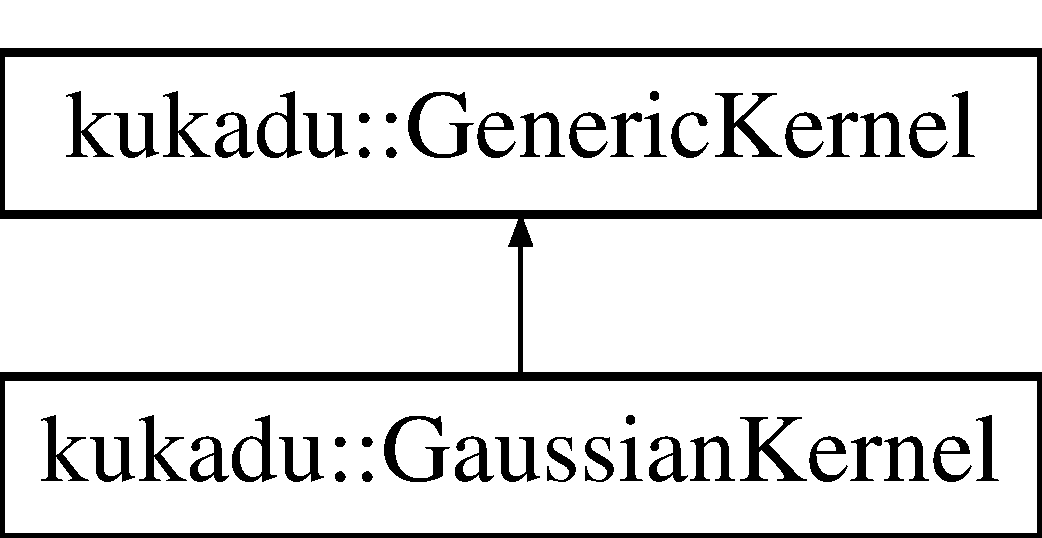
\includegraphics[height=2.000000cm]{classkukadu_1_1GaussianKernel}
\end{center}
\end{figure}
\subsection*{Public Member Functions}
\begin{DoxyCompactItemize}
\item 
\hyperlink{classkukadu_1_1GaussianKernel_a8f891d85494e0430cd5646bcd959585f}{Gaussian\-Kernel} (double theta0, double theta1)
\begin{DoxyCompactList}\small\item\em constructor \end{DoxyCompactList}\item 
double \hyperlink{classkukadu_1_1GaussianKernel_a11fec7aa4348f339008a454e268bf815}{evaluate\-Kernel} (arma\-::vec q1, arma\-::vec q2, void $\ast$kernel\-Param)
\begin{DoxyCompactList}\small\item\em computes kernel values with given vectors q1 and q2 and passes a not further specified kernel parameter that can be used by the kernel implementation \end{DoxyCompactList}\end{DoxyCompactItemize}


\subsection{Detailed Description}
Implements a Gaussian kernel according to the \hyperlink{classkukadu_1_1GenericKernel}{Generic\-Kernel} specifiction. 

This class implements a Gaussian kernel given by the function K(u) = theta0 e$^\wedge$(-\/ theta1 /2 u$^\wedge$2) 

\subsection{Constructor \& Destructor Documentation}
\hypertarget{classkukadu_1_1GaussianKernel_a8f891d85494e0430cd5646bcd959585f}{\index{kukadu\-::\-Gaussian\-Kernel@{kukadu\-::\-Gaussian\-Kernel}!Gaussian\-Kernel@{Gaussian\-Kernel}}
\index{Gaussian\-Kernel@{Gaussian\-Kernel}!kukadu::GaussianKernel@{kukadu\-::\-Gaussian\-Kernel}}
\subsubsection[{Gaussian\-Kernel}]{\setlength{\rightskip}{0pt plus 5cm}kukadu\-::\-Gaussian\-Kernel\-::\-Gaussian\-Kernel (
\begin{DoxyParamCaption}
\item[{double}]{theta0, }
\item[{double}]{theta1}
\end{DoxyParamCaption}
)}}\label{classkukadu_1_1GaussianKernel_a8f891d85494e0430cd5646bcd959585f}


constructor 


\begin{DoxyParams}{Parameters}
{\em theta0} & paremeter theta0 of the kernel according to the given kernel function \\
\hline
{\em theta1} & paremeter theta1 of the kernel according to the given kernel function \\
\hline
\end{DoxyParams}


\subsection{Member Function Documentation}
\hypertarget{classkukadu_1_1GaussianKernel_a11fec7aa4348f339008a454e268bf815}{\index{kukadu\-::\-Gaussian\-Kernel@{kukadu\-::\-Gaussian\-Kernel}!evaluate\-Kernel@{evaluate\-Kernel}}
\index{evaluate\-Kernel@{evaluate\-Kernel}!kukadu::GaussianKernel@{kukadu\-::\-Gaussian\-Kernel}}
\subsubsection[{evaluate\-Kernel}]{\setlength{\rightskip}{0pt plus 5cm}double kukadu\-::\-Gaussian\-Kernel\-::evaluate\-Kernel (
\begin{DoxyParamCaption}
\item[{arma\-::vec}]{q1, }
\item[{arma\-::vec}]{q2, }
\item[{void $\ast$}]{kernel\-Param}
\end{DoxyParamCaption}
)\hspace{0.3cm}{\ttfamily [virtual]}}}\label{classkukadu_1_1GaussianKernel_a11fec7aa4348f339008a454e268bf815}


computes kernel values with given vectors q1 and q2 and passes a not further specified kernel parameter that can be used by the kernel implementation 


\begin{DoxyParams}{Parameters}
{\em q1} & vector q1 with K = K(d(q1, q2)) \\
\hline
{\em q2} & vector q2 with K = K(d(q1, q2)) \\
\hline
{\em kernel\-Param} & arbitrary kernel parameter \\
\hline
\end{DoxyParams}


Implements \hyperlink{classkukadu_1_1GenericKernel_a802a15e8fb5f863e798c9114be976045}{kukadu\-::\-Generic\-Kernel}.



The documentation for this class was generated from the following files\-:\begin{DoxyCompactItemize}
\item 
/home/c7031109/iis\-\_\-robot\-\_\-sw/iis\-\_\-catkin\-\_\-ws/src/kukadu/include/kukadu/learning/regression/gaussiankernel.\-hpp\item 
/home/c7031109/iis\-\_\-robot\-\_\-sw/iis\-\_\-catkin\-\_\-ws/src/kukadu/src/learning/gaussiankernel.\-cpp\end{DoxyCompactItemize}

\hypertarget{classkukadu_1_1GaussianProcessRegressor}{\section{kukadu\-:\-:Gaussian\-Process\-Regressor Class Reference}
\label{classkukadu_1_1GaussianProcessRegressor}\index{kukadu\-::\-Gaussian\-Process\-Regressor@{kukadu\-::\-Gaussian\-Process\-Regressor}}
}


Implements the Gaussian process regression method.  




{\ttfamily \#include $<$gaussianprocessregressor.\-hpp$>$}

Inheritance diagram for kukadu\-:\-:Gaussian\-Process\-Regressor\-:\begin{figure}[H]
\begin{center}
\leavevmode
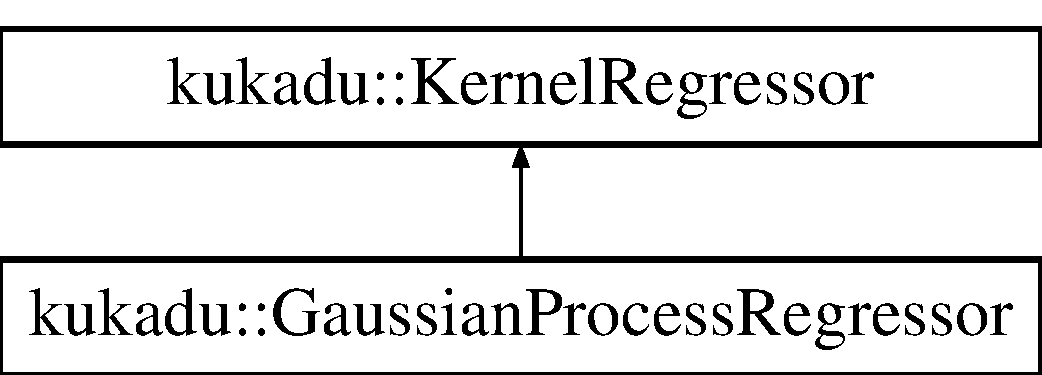
\includegraphics[height=2.000000cm]{classkukadu_1_1GaussianProcessRegressor}
\end{center}
\end{figure}
\subsection*{Public Member Functions}
\begin{DoxyCompactItemize}
\item 
\hyperlink{classkukadu_1_1GaussianProcessRegressor_a59721469c936e4352a28301ed3d8acc3}{Gaussian\-Process\-Regressor} (std\-::vector$<$ arma\-::vec $>$ sample\-Xs, arma\-::vec sample\-Ts, \hyperlink{classkukadu_1_1GenericKernel}{Generic\-Kernel} $\ast$kernel, double beta)
\begin{DoxyCompactList}\small\item\em constructor, setting all the sample data, the selected kernel and the variance beta \end{DoxyCompactList}\item 
arma\-::vec \hyperlink{classkukadu_1_1GaussianProcessRegressor_a397a1d055761ae22ec9edc3d311949ec}{fit\-At\-Position} (arma\-::vec pos)
\begin{DoxyCompactList}\small\item\em performs the kernel method for predicting the functin value at a given position \end{DoxyCompactList}\end{DoxyCompactItemize}


\subsection{Detailed Description}
Implements the Gaussian process regression method. 

This class inherits from the \hyperlink{classkukadu_1_1KernelRegressor}{Kernel\-Regressor} and implements Gaussian process regression. 

\subsection{Constructor \& Destructor Documentation}
\hypertarget{classkukadu_1_1GaussianProcessRegressor_a59721469c936e4352a28301ed3d8acc3}{\index{kukadu\-::\-Gaussian\-Process\-Regressor@{kukadu\-::\-Gaussian\-Process\-Regressor}!Gaussian\-Process\-Regressor@{Gaussian\-Process\-Regressor}}
\index{Gaussian\-Process\-Regressor@{Gaussian\-Process\-Regressor}!kukadu::GaussianProcessRegressor@{kukadu\-::\-Gaussian\-Process\-Regressor}}
\subsubsection[{Gaussian\-Process\-Regressor}]{\setlength{\rightskip}{0pt plus 5cm}kukadu\-::\-Gaussian\-Process\-Regressor\-::\-Gaussian\-Process\-Regressor (
\begin{DoxyParamCaption}
\item[{std\-::vector$<$ arma\-::vec $>$}]{sample\-Xs, }
\item[{arma\-::vec}]{sample\-Ts, }
\item[{{\bf Generic\-Kernel} $\ast$}]{kernel, }
\item[{double}]{beta}
\end{DoxyParamCaption}
)}}\label{classkukadu_1_1GaussianProcessRegressor_a59721469c936e4352a28301ed3d8acc3}


constructor, setting all the sample data, the selected kernel and the variance beta 


\begin{DoxyParams}{Parameters}
{\em sample\-Xs} & vector of samples (x-\/axis) \\
\hline
{\em sample\-Ts} & vector of samples (y-\/axis) \\
\hline
{\em kernel} & the selected kernel implementation \\
\hline
{\em beta} & the assumed sample variance \\
\hline
\end{DoxyParams}


\subsection{Member Function Documentation}
\hypertarget{classkukadu_1_1GaussianProcessRegressor_a397a1d055761ae22ec9edc3d311949ec}{\index{kukadu\-::\-Gaussian\-Process\-Regressor@{kukadu\-::\-Gaussian\-Process\-Regressor}!fit\-At\-Position@{fit\-At\-Position}}
\index{fit\-At\-Position@{fit\-At\-Position}!kukadu::GaussianProcessRegressor@{kukadu\-::\-Gaussian\-Process\-Regressor}}
\subsubsection[{fit\-At\-Position}]{\setlength{\rightskip}{0pt plus 5cm}vec kukadu\-::\-Gaussian\-Process\-Regressor\-::fit\-At\-Position (
\begin{DoxyParamCaption}
\item[{arma\-::vec}]{pos}
\end{DoxyParamCaption}
)\hspace{0.3cm}{\ttfamily [virtual]}}}\label{classkukadu_1_1GaussianProcessRegressor_a397a1d055761ae22ec9edc3d311949ec}


performs the kernel method for predicting the functin value at a given position 


\begin{DoxyParams}{Parameters}
{\em pos} & vector defining the required position \\
\hline
\end{DoxyParams}


Implements \hyperlink{classkukadu_1_1KernelRegressor_afd1489310e11cff4bd88390ba76c38e1}{kukadu\-::\-Kernel\-Regressor}.



The documentation for this class was generated from the following files\-:\begin{DoxyCompactItemize}
\item 
/home/c7031109/iis\-\_\-robot\-\_\-sw/iis\-\_\-catkin\-\_\-ws/src/kukadu/include/kukadu/learning/regression/gaussianprocessregressor.\-hpp\item 
/home/c7031109/iis\-\_\-robot\-\_\-sw/iis\-\_\-catkin\-\_\-ws/src/kukadu/src/learning/gaussianprocessregressor.\-cpp\end{DoxyCompactItemize}

\hypertarget{classkukadu_1_1GeneralDmpLearner}{\section{kukadu\-:\-:General\-Dmp\-Learner Class Reference}
\label{classkukadu_1_1GeneralDmpLearner}\index{kukadu\-::\-General\-Dmp\-Learner@{kukadu\-::\-General\-Dmp\-Learner}}
}
Inheritance diagram for kukadu\-:\-:General\-Dmp\-Learner\-:\begin{figure}[H]
\begin{center}
\leavevmode
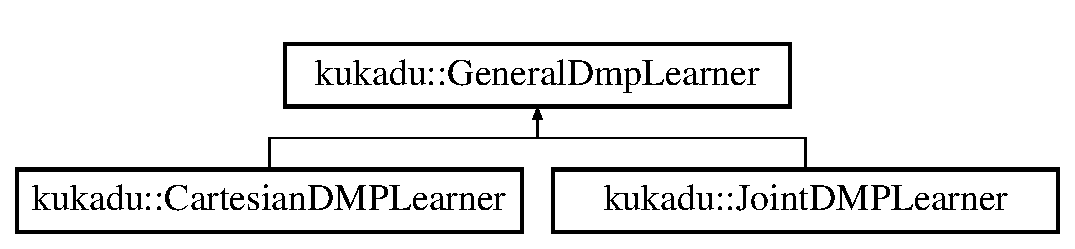
\includegraphics[height=2.000000cm]{classkukadu_1_1GeneralDmpLearner}
\end{center}
\end{figure}
\subsection*{Public Member Functions}
\begin{DoxyCompactItemize}
\item 
\hyperlink{classkukadu_1_1GeneralDmpLearner_a267ea59435a0bf8e2b29ad06fbb07122}{General\-Dmp\-Learner} (std\-::vector$<$ \hyperlink{classkukadu_1_1DMPBase}{D\-M\-P\-Base} $>$ dmp\-Base, double tau, double az, double bz, double ax, arma\-::mat joints)
\begin{DoxyCompactList}\small\item\em constructor \end{DoxyCompactList}\item 
\hyperlink{classkukadu_1_1GeneralDmpLearner_a317520b316d8d6e75206237f0848b3c1}{General\-Dmp\-Learner} (std\-::vector$<$ double $>$ mys\-Def, std\-::vector$<$ double $>$ sigmas\-Def, double az, double bz, std\-::string file)
\begin{DoxyCompactList}\small\item\em constructor \end{DoxyCompactList}\item 
\hypertarget{classkukadu_1_1GeneralDmpLearner_ab9adb95165d0799c1abe7038b088c419}{{\bfseries General\-Dmp\-Learner} (double az, double bz, std\-::string file)}\label{classkukadu_1_1GeneralDmpLearner_ab9adb95165d0799c1abe7038b088c419}

\item 
\hypertarget{classkukadu_1_1GeneralDmpLearner_afc0a3a13e70d079cc33ee157b2e8adfe}{{\bfseries General\-Dmp\-Learner} (double az, double bz, arma\-::mat joints)}\label{classkukadu_1_1GeneralDmpLearner_afc0a3a13e70d079cc33ee157b2e8adfe}

\item 
\hypertarget{classkukadu_1_1GeneralDmpLearner_a4f2f314a7bfb0d9ff54fabbb038757c8}{K\-U\-K\-A\-D\-U\-\_\-\-S\-H\-A\-R\-E\-D\-\_\-\-P\-T\-R$<$ \hyperlink{classkukadu_1_1Dmp}{Dmp} $>$ \hyperlink{classkukadu_1_1GeneralDmpLearner_a4f2f314a7bfb0d9ff54fabbb038757c8}{fit\-Trajectories} ()}\label{classkukadu_1_1GeneralDmpLearner_a4f2f314a7bfb0d9ff54fabbb038757c8}

\begin{DoxyCompactList}\small\item\em fit the specified trajectories \end{DoxyCompactList}\end{DoxyCompactItemize}
\subsection*{Protected Member Functions}
\begin{DoxyCompactItemize}
\item 
\hypertarget{classkukadu_1_1GeneralDmpLearner_a817dca6e1bf76da6937e711300ee9226}{virtual K\-U\-K\-A\-D\-U\-\_\-\-S\-H\-A\-R\-E\-D\-\_\-\-P\-T\-R$<$ \hyperlink{classkukadu_1_1Dmp}{Dmp} $>$ {\bfseries create\-Dmp\-Instance} (arma\-::vec supervised\-Ts, std\-::vector$<$ arma\-::vec $>$ sample\-Ys, std\-::vector$<$ arma\-::vec $>$ fit\-Ys, std\-::vector$<$ arma\-::vec $>$ dmp\-Coeffs, std\-::vector$<$ \hyperlink{classkukadu_1_1DMPBase}{D\-M\-P\-Base} $>$ dmp\-Base, std\-::vector$<$ arma\-::mat $>$ design\-Matrices, double tau, double az, double bz, double ax)=0}\label{classkukadu_1_1GeneralDmpLearner_a817dca6e1bf76da6937e711300ee9226}

\item 
\hypertarget{classkukadu_1_1GeneralDmpLearner_a5df8ee4640adf585cbce7b04e77ae3a6}{virtual arma\-::mat {\bfseries compute\-Fit\-Y} (arma\-::vec \&time, arma\-::mat \&y, arma\-::mat \&dy, arma\-::mat \&ddy, arma\-::vec \&vec\-\_\-g)=0}\label{classkukadu_1_1GeneralDmpLearner_a5df8ee4640adf585cbce7b04e77ae3a6}

\end{DoxyCompactItemize}
\subsection*{Protected Attributes}
\begin{DoxyCompactItemize}
\item 
\hypertarget{classkukadu_1_1GeneralDmpLearner_abccf72154087561579ce0abe1ff85ff3}{double {\bfseries az}}\label{classkukadu_1_1GeneralDmpLearner_abccf72154087561579ce0abe1ff85ff3}

\item 
\hypertarget{classkukadu_1_1GeneralDmpLearner_ad910f3a86c8551f63c643347ae4f15fe}{double {\bfseries bz}}\label{classkukadu_1_1GeneralDmpLearner_ad910f3a86c8551f63c643347ae4f15fe}

\item 
\hypertarget{classkukadu_1_1GeneralDmpLearner_ab6b6b3fa49ef6c7925dbe34ea5991f48}{double {\bfseries ax}}\label{classkukadu_1_1GeneralDmpLearner_ab6b6b3fa49ef6c7925dbe34ea5991f48}

\item 
\hypertarget{classkukadu_1_1GeneralDmpLearner_af27b307365984e9deae829ca2159ed57}{double {\bfseries tau}}\label{classkukadu_1_1GeneralDmpLearner_af27b307365984e9deae829ca2159ed57}

\end{DoxyCompactItemize}


\subsection{Constructor \& Destructor Documentation}
\hypertarget{classkukadu_1_1GeneralDmpLearner_a267ea59435a0bf8e2b29ad06fbb07122}{\index{kukadu\-::\-General\-Dmp\-Learner@{kukadu\-::\-General\-Dmp\-Learner}!General\-Dmp\-Learner@{General\-Dmp\-Learner}}
\index{General\-Dmp\-Learner@{General\-Dmp\-Learner}!kukadu::GeneralDmpLearner@{kukadu\-::\-General\-Dmp\-Learner}}
\subsubsection[{General\-Dmp\-Learner}]{\setlength{\rightskip}{0pt plus 5cm}kukadu\-::\-General\-Dmp\-Learner\-::\-General\-Dmp\-Learner (
\begin{DoxyParamCaption}
\item[{std\-::vector$<$ {\bf D\-M\-P\-Base} $>$}]{dmp\-Base, }
\item[{double}]{tau, }
\item[{double}]{az, }
\item[{double}]{bz, }
\item[{double}]{ax, }
\item[{arma\-::mat}]{joints}
\end{DoxyParamCaption}
)}}\label{classkukadu_1_1GeneralDmpLearner_a267ea59435a0bf8e2b29ad06fbb07122}


constructor 


\begin{DoxyParams}{Parameters}
{\em dmp\-Base} & dmp basis function definition \\
\hline
{\em tau} & dmp timing constant \\
\hline
{\em az} & dmp az constant \\
\hline
{\em bz} & dmp bz constant \\
\hline
{\em ax} & dmp ax constant \\
\hline
{\em joints} & measured joints \\
\hline
{\em deg\-Freedom} & robots degrees of freedom \\
\hline
\end{DoxyParams}
\hypertarget{classkukadu_1_1GeneralDmpLearner_a317520b316d8d6e75206237f0848b3c1}{\index{kukadu\-::\-General\-Dmp\-Learner@{kukadu\-::\-General\-Dmp\-Learner}!General\-Dmp\-Learner@{General\-Dmp\-Learner}}
\index{General\-Dmp\-Learner@{General\-Dmp\-Learner}!kukadu::GeneralDmpLearner@{kukadu\-::\-General\-Dmp\-Learner}}
\subsubsection[{General\-Dmp\-Learner}]{\setlength{\rightskip}{0pt plus 5cm}kukadu\-::\-General\-Dmp\-Learner\-::\-General\-Dmp\-Learner (
\begin{DoxyParamCaption}
\item[{std\-::vector$<$ double $>$}]{mys\-Def, }
\item[{std\-::vector$<$ double $>$}]{sigmas\-Def, }
\item[{double}]{az, }
\item[{double}]{bz, }
\item[{std\-::string}]{file}
\end{DoxyParamCaption}
)}}\label{classkukadu_1_1GeneralDmpLearner_a317520b316d8d6e75206237f0848b3c1}


constructor 


\begin{DoxyParams}{Parameters}
{\em dmp\-Base} & dmp basis function definition \\
\hline
{\em tau} & dmp timing constant \\
\hline
{\em az} & dmp az constant \\
\hline
{\em bz} & dmp bz constant \\
\hline
{\em ax} & dmp ax constant \\
\hline
{\em file} & file containing the measured joints \\
\hline
{\em deg\-Freedom} & robots degrees of freedom \\
\hline
\end{DoxyParams}


The documentation for this class was generated from the following files\-:\begin{DoxyCompactItemize}
\item 
/home/c7031109/iis\-\_\-robot\-\_\-sw/iis\-\_\-catkin\-\_\-ws/src/kukadu/include/kukadu/control/generaldmplearner.\-hpp\item 
/home/c7031109/iis\-\_\-robot\-\_\-sw/iis\-\_\-catkin\-\_\-ws/src/kukadu/src/control/generaldmplearner.\-cpp\end{DoxyCompactItemize}

\hypertarget{classkukadu_1_1GeneralFitter}{\section{kukadu\-:\-:General\-Fitter Class Reference}
\label{classkukadu_1_1GeneralFitter}\index{kukadu\-::\-General\-Fitter@{kukadu\-::\-General\-Fitter}}
}


Provides the generic part of the linear regression methods.  




{\ttfamily \#include $<$generalfitter.\-hpp$>$}

\subsection*{Public Member Functions}
\begin{DoxyCompactItemize}
\item 
\hyperlink{classkukadu_1_1GeneralFitter_a6546135463b8ae78e707a5538166d545}{General\-Fitter} (arma\-::vec samples\-X, arma\-::vec samples\-Y, int sample\-Count, \hyperlink{classkukadu_1_1TrajectoryGenerator}{Trajectory\-Generator} $\ast$traj\-Gen)
\begin{DoxyCompactList}\small\item\em constructor \end{DoxyCompactList}\item 
\hypertarget{classkukadu_1_1GeneralFitter_ac87a8f6d6e036c424dd022808876421f}{int \hyperlink{classkukadu_1_1GeneralFitter_ac87a8f6d6e036c424dd022808876421f}{get\-Basis\-Function\-Count} ()}\label{classkukadu_1_1GeneralFitter_ac87a8f6d6e036c424dd022808876421f}

\begin{DoxyCompactList}\small\item\em returns the number of basis functions \end{DoxyCompactList}\item 
\hypertarget{classkukadu_1_1GeneralFitter_ab5aad99091bf484941090ce2dcaf9881}{int \hyperlink{classkukadu_1_1GeneralFitter_ab5aad99091bf484941090ce2dcaf9881}{get\-Sample\-Count} ()}\label{classkukadu_1_1GeneralFitter_ab5aad99091bf484941090ce2dcaf9881}

\begin{DoxyCompactList}\small\item\em returns the number of samples \end{DoxyCompactList}\item 
\hypertarget{classkukadu_1_1GeneralFitter_ad83ff2da0b13813710684596ee4e28df}{arma\-::vec \hyperlink{classkukadu_1_1GeneralFitter_ad83ff2da0b13813710684596ee4e28df}{compute\-Lin\-Fit\-Coefficients} ()}\label{classkukadu_1_1GeneralFitter_ad83ff2da0b13813710684596ee4e28df}

\begin{DoxyCompactList}\small\item\em performs linear regression and returns vector of coefficients corresponding to the basis functions \end{DoxyCompactList}\item 
arma\-::vec \hyperlink{classkukadu_1_1GeneralFitter_ababdab99ea68030d3fa7b5cd692e4372}{compute\-Lin\-Fit\-Coefficients} (arma\-::mat des\-Mat)
\begin{DoxyCompactList}\small\item\em performs linear regression and returns vector of coefficients corresponding to the basis functions by explicitly taking the design matrix as parameter \end{DoxyCompactList}\item 
\hypertarget{classkukadu_1_1GeneralFitter_aa1b7d37f59d0c86185425ec550e6c1b0}{arma\-::mat \hyperlink{classkukadu_1_1GeneralFitter_aa1b7d37f59d0c86185425ec550e6c1b0}{compute\-Design\-Matrix} ()}\label{classkukadu_1_1GeneralFitter_aa1b7d37f59d0c86185425ec550e6c1b0}

\begin{DoxyCompactList}\small\item\em computes design matrix \end{DoxyCompactList}\end{DoxyCompactItemize}


\subsection{Detailed Description}
Provides the generic part of the linear regression methods. 

This class provides implements the generic part of the linear regression method. It is independent of the specific choice of basis functions. These basis functions are defined via the \hyperlink{classkukadu_1_1TrajectoryGenerator}{Trajectory\-Generator} class. 

\subsection{Constructor \& Destructor Documentation}
\hypertarget{classkukadu_1_1GeneralFitter_a6546135463b8ae78e707a5538166d545}{\index{kukadu\-::\-General\-Fitter@{kukadu\-::\-General\-Fitter}!General\-Fitter@{General\-Fitter}}
\index{General\-Fitter@{General\-Fitter}!kukadu::GeneralFitter@{kukadu\-::\-General\-Fitter}}
\subsubsection[{General\-Fitter}]{\setlength{\rightskip}{0pt plus 5cm}kukadu\-::\-General\-Fitter\-::\-General\-Fitter (
\begin{DoxyParamCaption}
\item[{arma\-::vec}]{samples\-X, }
\item[{arma\-::vec}]{samples\-Y, }
\item[{int}]{sample\-Count, }
\item[{{\bf Trajectory\-Generator} $\ast$}]{traj\-Gen}
\end{DoxyParamCaption}
)}}\label{classkukadu_1_1GeneralFitter_a6546135463b8ae78e707a5538166d545}


constructor 


\begin{DoxyParams}{Parameters}
{\em samples\-X} & vector of samples, where samples\-X specifies the x-\/axis \\
\hline
{\em samples\-Y} & vector of samples, where samples\-Y specifies the y-\/axis \\
\hline
{\em sample\-Count} & number of sample points \\
\hline
{\em traj\-Gen} & \hyperlink{classkukadu_1_1TrajectoryGenerator}{Trajectory\-Generator} instance defining the basis functions \\
\hline
\end{DoxyParams}


\subsection{Member Function Documentation}
\hypertarget{classkukadu_1_1GeneralFitter_ababdab99ea68030d3fa7b5cd692e4372}{\index{kukadu\-::\-General\-Fitter@{kukadu\-::\-General\-Fitter}!compute\-Lin\-Fit\-Coefficients@{compute\-Lin\-Fit\-Coefficients}}
\index{compute\-Lin\-Fit\-Coefficients@{compute\-Lin\-Fit\-Coefficients}!kukadu::GeneralFitter@{kukadu\-::\-General\-Fitter}}
\subsubsection[{compute\-Lin\-Fit\-Coefficients}]{\setlength{\rightskip}{0pt plus 5cm}arma\-::vec kukadu\-::\-General\-Fitter\-::compute\-Lin\-Fit\-Coefficients (
\begin{DoxyParamCaption}
\item[{arma\-::mat}]{des\-Mat}
\end{DoxyParamCaption}
)}}\label{classkukadu_1_1GeneralFitter_ababdab99ea68030d3fa7b5cd692e4372}


performs linear regression and returns vector of coefficients corresponding to the basis functions by explicitly taking the design matrix as parameter 


\begin{DoxyParams}{Parameters}
{\em des\-Mat} & design matrix needed for linear regression \\
\hline
\end{DoxyParams}


The documentation for this class was generated from the following files\-:\begin{DoxyCompactItemize}
\item 
/home/c7031109/iis\-\_\-robot\-\_\-sw/iis\-\_\-catkin\-\_\-ws/src/kukadu/include/kukadu/learning/regression/generalfitter.\-hpp\item 
/home/c7031109/iis\-\_\-robot\-\_\-sw/iis\-\_\-catkin\-\_\-ws/src/kukadu/src/learning/generalfitter.\-cpp\end{DoxyCompactItemize}

\hypertarget{classkukadu_1_1GeneralReinforcer}{\section{kukadu\-:\-:General\-Reinforcer Class Reference}
\label{classkukadu_1_1GeneralReinforcer}\index{kukadu\-::\-General\-Reinforcer@{kukadu\-::\-General\-Reinforcer}}
}


The \hyperlink{classkukadu_1_1GeneralReinforcer}{General\-Reinforcer} provides a general framework for reinforcement learning.  




{\ttfamily \#include $<$generalreinforcer.\-hpp$>$}

Inheritance diagram for kukadu\-:\-:General\-Reinforcer\-:\begin{figure}[H]
\begin{center}
\leavevmode
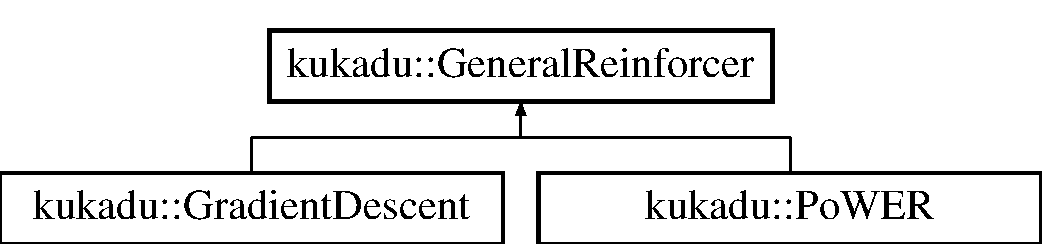
\includegraphics[height=2.000000cm]{classkukadu_1_1GeneralReinforcer}
\end{center}
\end{figure}
\subsection*{Public Member Functions}
\begin{DoxyCompactItemize}
\item 
\hyperlink{classkukadu_1_1GeneralReinforcer_a1de3f2b46e82b37454f8095701992c8d}{General\-Reinforcer} (K\-U\-K\-A\-D\-U\-\_\-\-S\-H\-A\-R\-E\-D\-\_\-\-P\-T\-R$<$ \hyperlink{classkukadu_1_1TrajectoryExecutor}{Trajectory\-Executor} $>$ traj\-Ex, K\-U\-K\-A\-D\-U\-\_\-\-S\-H\-A\-R\-E\-D\-\_\-\-P\-T\-R$<$ \hyperlink{classkukadu_1_1CostComputer}{Cost\-Computer} $>$ cost, K\-U\-K\-A\-D\-U\-\_\-\-S\-H\-A\-R\-E\-D\-\_\-\-P\-T\-R$<$ \hyperlink{classkukadu_1_1ControlQueue}{Control\-Queue} $>$ simulation\-Queue, K\-U\-K\-A\-D\-U\-\_\-\-S\-H\-A\-R\-E\-D\-\_\-\-P\-T\-R$<$ \hyperlink{classkukadu_1_1ControlQueue}{Control\-Queue} $>$ execution\-Queue)
\begin{DoxyCompactList}\small\item\em constructor \end{DoxyCompactList}\item 
\hypertarget{classkukadu_1_1GeneralReinforcer_aa384f66bcf7487b449dc67c768e86f5e}{bool \hyperlink{classkukadu_1_1GeneralReinforcer_aa384f66bcf7487b449dc67c768e86f5e}{get\-Is\-First\-Iteration} ()}\label{classkukadu_1_1GeneralReinforcer_aa384f66bcf7487b449dc67c768e86f5e}

\begin{DoxyCompactList}\small\item\em returns true if the first iteration has not been performed yet \end{DoxyCompactList}\item 
void \hyperlink{classkukadu_1_1GeneralReinforcer_aee9cbeaac91379e1926088150f9c5063}{perform\-Rollout} (int do\-Simulation, int do\-Execution)
\begin{DoxyCompactList}\small\item\em executes rollout. first, the trajectory is simulated and the user is asked, whether the trajectory really should be executed \end{DoxyCompactList}\item 
\hypertarget{classkukadu_1_1GeneralReinforcer_a0fe9f486ada94bb1eeeb6e460da5579f}{void {\bfseries set\-Last\-Update} (K\-U\-K\-A\-D\-U\-\_\-\-S\-H\-A\-R\-E\-D\-\_\-\-P\-T\-R$<$ \hyperlink{classkukadu_1_1Trajectory}{Trajectory} $>$ last\-Update)}\label{classkukadu_1_1GeneralReinforcer_a0fe9f486ada94bb1eeeb6e460da5579f}

\item 
\hypertarget{classkukadu_1_1GeneralReinforcer_aa65904e99bffab1272d49b01d515a670}{double {\bfseries get\-Last\-Update\-Reward} ()}\label{classkukadu_1_1GeneralReinforcer_aa65904e99bffab1272d49b01d515a670}

\item 
\hypertarget{classkukadu_1_1GeneralReinforcer_a19213b562d0a5a0320347e51ae108f9e}{K\-U\-K\-A\-D\-U\-\_\-\-S\-H\-A\-R\-E\-D\-\_\-\-P\-T\-R$<$ \hyperlink{classkukadu_1_1Trajectory}{Trajectory} $>$ {\bfseries get\-Last\-Update} ()}\label{classkukadu_1_1GeneralReinforcer_a19213b562d0a5a0320347e51ae108f9e}

\item 
\hypertarget{classkukadu_1_1GeneralReinforcer_a7aa17bfed379c5673d81eb17db4b4932}{K\-U\-K\-A\-D\-U\-\_\-\-S\-H\-A\-R\-E\-D\-\_\-\-P\-T\-R\\*
$<$ \hyperlink{classkukadu_1_1ControllerResult}{Controller\-Result} $>$ {\bfseries get\-Last\-Update\-Res} ()}\label{classkukadu_1_1GeneralReinforcer_a7aa17bfed379c5673d81eb17db4b4932}

\item 
\hypertarget{classkukadu_1_1GeneralReinforcer_a5c26cdef91f856f34c528547eee94472}{std\-::vector$<$ double $>$ \hyperlink{classkukadu_1_1GeneralReinforcer_a5c26cdef91f856f34c528547eee94472}{get\-Last\-Rollout\-Cost} ()}\label{classkukadu_1_1GeneralReinforcer_a5c26cdef91f856f34c528547eee94472}

\begin{DoxyCompactList}\small\item\em returns cost for the last executed rollout \end{DoxyCompactList}\item 
\hypertarget{classkukadu_1_1GeneralReinforcer_a4223bf864a5fe99bd42fe92c7e453869}{std\-::vector$<$ K\-U\-K\-A\-D\-U\-\_\-\-S\-H\-A\-R\-E\-D\-\_\-\-P\-T\-R\\*
$<$ \hyperlink{classkukadu_1_1Trajectory}{Trajectory} $>$ $>$ {\bfseries get\-Last\-Rollout\-Parameters} ()}\label{classkukadu_1_1GeneralReinforcer_a4223bf864a5fe99bd42fe92c7e453869}

\item 
\hypertarget{classkukadu_1_1GeneralReinforcer_a1ed63236a3d31d26152ffb9f01f5363a}{std\-::vector$<$ K\-U\-K\-A\-D\-U\-\_\-\-S\-H\-A\-R\-E\-D\-\_\-\-P\-T\-R\\*
$<$ \hyperlink{classkukadu_1_1ControllerResult}{Controller\-Result} $>$ $>$ {\bfseries get\-Last\-Execution\-Results} ()}\label{classkukadu_1_1GeneralReinforcer_a1ed63236a3d31d26152ffb9f01f5363a}

\item 
\hypertarget{classkukadu_1_1GeneralReinforcer_a2925052d641e845dba068fa03d567b20}{virtual K\-U\-K\-A\-D\-U\-\_\-\-S\-H\-A\-R\-E\-D\-\_\-\-P\-T\-R\\*
$<$ \hyperlink{classkukadu_1_1Trajectory}{Trajectory} $>$ {\bfseries update\-Step} ()=0}\label{classkukadu_1_1GeneralReinforcer_a2925052d641e845dba068fa03d567b20}

\item 
\hypertarget{classkukadu_1_1GeneralReinforcer_aa7e72994ca8c009d1331129480d2e49f}{virtual std\-::vector\\*
$<$ K\-U\-K\-A\-D\-U\-\_\-\-S\-H\-A\-R\-E\-D\-\_\-\-P\-T\-R\\*
$<$ \hyperlink{classkukadu_1_1Trajectory}{Trajectory} $>$ $>$ \hyperlink{classkukadu_1_1GeneralReinforcer_aa7e72994ca8c009d1331129480d2e49f}{get\-Initial\-Rollout} ()=0}\label{classkukadu_1_1GeneralReinforcer_aa7e72994ca8c009d1331129480d2e49f}

\begin{DoxyCompactList}\small\item\em returns the first rollout of the reinforcement learning algorithm \end{DoxyCompactList}\item 
\hypertarget{classkukadu_1_1GeneralReinforcer_aec3cde390852d93c52a01926bbc6feb3}{virtual std\-::vector\\*
$<$ K\-U\-K\-A\-D\-U\-\_\-\-S\-H\-A\-R\-E\-D\-\_\-\-P\-T\-R\\*
$<$ \hyperlink{classkukadu_1_1Trajectory}{Trajectory} $>$ $>$ \hyperlink{classkukadu_1_1GeneralReinforcer_aec3cde390852d93c52a01926bbc6feb3}{compute\-Rollout\-Paramters} ()=0}\label{classkukadu_1_1GeneralReinforcer_aec3cde390852d93c52a01926bbc6feb3}

\begin{DoxyCompactList}\small\item\em computes the dmp parameters for the next rollout \end{DoxyCompactList}\end{DoxyCompactItemize}


\subsection{Detailed Description}
The \hyperlink{classkukadu_1_1GeneralReinforcer}{General\-Reinforcer} provides a general framework for reinforcement learning. 

It is an abstract class that implements elementary functionality that should be in common for all reinforcement learning methods (such as rollout execution). A concrete implementation of the \hyperlink{classkukadu_1_1DMPReinforcer}{D\-M\-P\-Reinforcer} has to implement the missing parts such as the methods get\-Initial\-Rollout and compute\-Rollout\-Paramters. 

\subsection{Constructor \& Destructor Documentation}
\hypertarget{classkukadu_1_1GeneralReinforcer_a1de3f2b46e82b37454f8095701992c8d}{\index{kukadu\-::\-General\-Reinforcer@{kukadu\-::\-General\-Reinforcer}!General\-Reinforcer@{General\-Reinforcer}}
\index{General\-Reinforcer@{General\-Reinforcer}!kukadu::GeneralReinforcer@{kukadu\-::\-General\-Reinforcer}}
\subsubsection[{General\-Reinforcer}]{\setlength{\rightskip}{0pt plus 5cm}kukadu\-::\-General\-Reinforcer\-::\-General\-Reinforcer (
\begin{DoxyParamCaption}
\item[{K\-U\-K\-A\-D\-U\-\_\-\-S\-H\-A\-R\-E\-D\-\_\-\-P\-T\-R$<$ {\bf Trajectory\-Executor} $>$}]{traj\-Ex, }
\item[{K\-U\-K\-A\-D\-U\-\_\-\-S\-H\-A\-R\-E\-D\-\_\-\-P\-T\-R$<$ {\bf Cost\-Computer} $>$}]{cost, }
\item[{K\-U\-K\-A\-D\-U\-\_\-\-S\-H\-A\-R\-E\-D\-\_\-\-P\-T\-R$<$ {\bf Control\-Queue} $>$}]{simulation\-Queue, }
\item[{K\-U\-K\-A\-D\-U\-\_\-\-S\-H\-A\-R\-E\-D\-\_\-\-P\-T\-R$<$ {\bf Control\-Queue} $>$}]{execution\-Queue}
\end{DoxyParamCaption}
)}}\label{classkukadu_1_1GeneralReinforcer_a1de3f2b46e82b37454f8095701992c8d}


constructor 


\begin{DoxyParams}{Parameters}
{\em cost} & \hyperlink{classkukadu_1_1CostComputer}{Cost\-Computer} instance that computes the cost of a given rollout \\
\hline
{\em movement\-Queue} & \hyperlink{classkukadu_1_1ControlQueue}{Control\-Queue} instance for robot execution \\
\hline
{\em ac} & dmp phase stopping parameter \\
\hline
{\em dmp\-Step\-Size} & step size for dmp execution \\
\hline
{\em tol\-Abs\-Err} & absolute tolerated error for numerical approximation \\
\hline
{\em tol\-Rel\-Err} & relative tolerated error for numerical approximation \\
\hline
\end{DoxyParams}


\subsection{Member Function Documentation}
\hypertarget{classkukadu_1_1GeneralReinforcer_aee9cbeaac91379e1926088150f9c5063}{\index{kukadu\-::\-General\-Reinforcer@{kukadu\-::\-General\-Reinforcer}!perform\-Rollout@{perform\-Rollout}}
\index{perform\-Rollout@{perform\-Rollout}!kukadu::GeneralReinforcer@{kukadu\-::\-General\-Reinforcer}}
\subsubsection[{perform\-Rollout}]{\setlength{\rightskip}{0pt plus 5cm}void kukadu\-::\-General\-Reinforcer\-::perform\-Rollout (
\begin{DoxyParamCaption}
\item[{int}]{do\-Simulation, }
\item[{int}]{do\-Execution}
\end{DoxyParamCaption}
)}}\label{classkukadu_1_1GeneralReinforcer_aee9cbeaac91379e1926088150f9c5063}


executes rollout. first, the trajectory is simulated and the user is asked, whether the trajectory really should be executed 


\begin{DoxyParams}{Parameters}
{\em do\-Simulation} & flag whether trajectory should be simulated \\
\hline
{\em do\-Execution} & flag whether trajectory should be executed at robot \\
\hline
\end{DoxyParams}


The documentation for this class was generated from the following files\-:\begin{DoxyCompactItemize}
\item 
/home/c7031109/iis\-\_\-robot\-\_\-sw/iis\-\_\-catkin\-\_\-ws/src/kukadu/include/kukadu/learning/rl/generalreinforcer.\-hpp\item 
/home/c7031109/iis\-\_\-robot\-\_\-sw/iis\-\_\-catkin\-\_\-ws/src/kukadu/src/learning/reinforcement\-\_\-learning/generalreinforcer.\-cpp\end{DoxyCompactItemize}

\hypertarget{classkukadu_1_1GenericGeneralizer}{\section{kukadu\-:\-:Generic\-Generalizer Class Reference}
\label{classkukadu_1_1GenericGeneralizer}\index{kukadu\-::\-Generic\-Generalizer@{kukadu\-::\-Generic\-Generalizer}}
}
Inheritance diagram for kukadu\-:\-:Generic\-Generalizer\-:\begin{figure}[H]
\begin{center}
\leavevmode
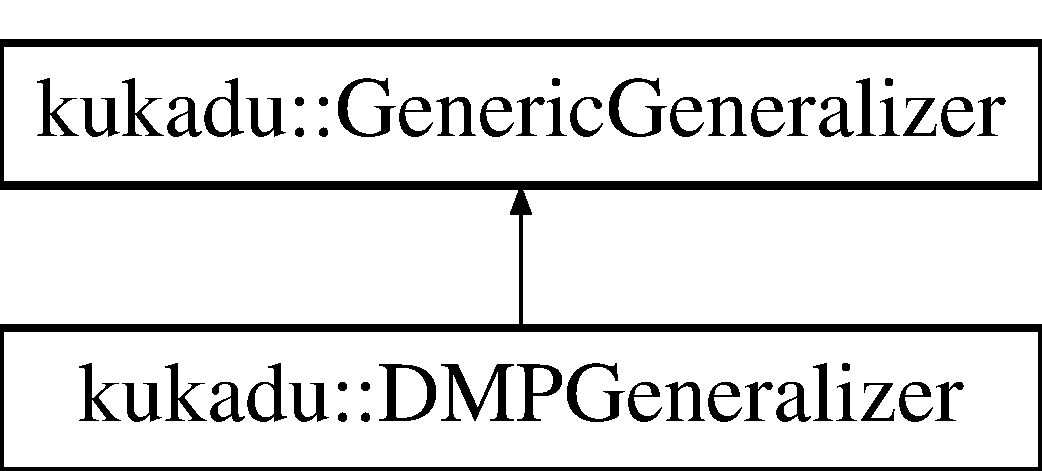
\includegraphics[height=2.000000cm]{classkukadu_1_1GenericGeneralizer}
\end{center}
\end{figure}
\subsection*{Public Member Functions}
\begin{DoxyCompactItemize}
\item 
\hypertarget{classkukadu_1_1GenericGeneralizer_a39874ac4acbf59957ba81f3ba2f620cd}{virtual K\-U\-K\-A\-D\-U\-\_\-\-S\-H\-A\-R\-E\-D\-\_\-\-P\-T\-R\\*
$<$ \hyperlink{classkukadu_1_1JointDmp}{Joint\-Dmp} $>$ {\bfseries generalize\-Dmp} (\hyperlink{classkukadu_1_1GenericKernel}{Generic\-Kernel} $\ast$trajectory\-Kernel, \hyperlink{classkukadu_1_1GenericKernel}{Generic\-Kernel} $\ast$parameter\-Kernel, arma\-::vec query, double beta)=0}\label{classkukadu_1_1GenericGeneralizer_a39874ac4acbf59957ba81f3ba2f620cd}

\end{DoxyCompactItemize}


The documentation for this class was generated from the following file\-:\begin{DoxyCompactItemize}
\item 
/home/c7031109/iis\-\_\-robot\-\_\-sw/iis\-\_\-catkin\-\_\-ws/src/kukadu/include/kukadu/control/genericgeneralizer.\-hpp\end{DoxyCompactItemize}

\hypertarget{classkukadu_1_1GenericHand}{\section{kukadu\-:\-:Generic\-Hand Class Reference}
\label{classkukadu_1_1GenericHand}\index{kukadu\-::\-Generic\-Hand@{kukadu\-::\-Generic\-Hand}}
}


The \hyperlink{classkukadu_1_1GenericHand}{Generic\-Hand} provides a very elementary interface to control robot hands mounted on a robot arm This class provides very an interface for the very basic functionalities such as \char`\"{}connect to hand\char`\"{} or \char`\"{}close hand\char`\"{}.  




{\ttfamily \#include $<$generichand.\-hpp$>$}

Inheritance diagram for kukadu\-:\-:Generic\-Hand\-:\begin{figure}[H]
\begin{center}
\leavevmode
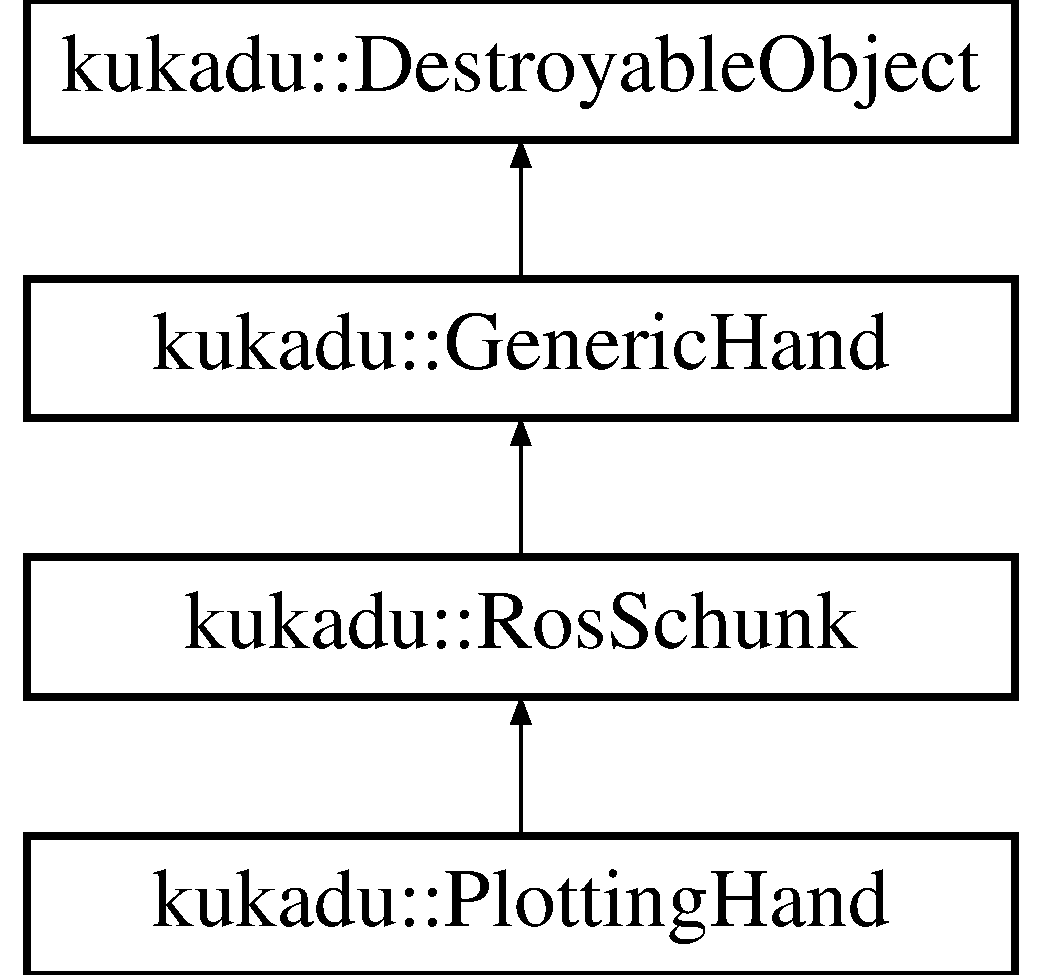
\includegraphics[height=4.000000cm]{classkukadu_1_1GenericHand}
\end{center}
\end{figure}
\subsection*{Public Member Functions}
\begin{DoxyCompactItemize}
\item 
virtual void \hyperlink{classkukadu_1_1GenericHand_a965ed8a8d225fb36eabf5089fa5d4f32}{connect\-Hand} ()=0
\begin{DoxyCompactList}\small\item\em Initializes the connection to the hand. \end{DoxyCompactList}\item 
virtual void \hyperlink{classkukadu_1_1GenericHand_a000e4d03e93f50d7101c50e6096d28a0}{close\-Hand} (double percentage, double velocity)=0
\begin{DoxyCompactList}\small\item\em Opens and closes the hand according to the provided closing percentage and velocity. \end{DoxyCompactList}\item 
\hypertarget{classkukadu_1_1GenericHand_a7662305094e40833ef22e6675e41c5fd}{virtual void {\bfseries move\-Joints} (arma\-::vec joints)=0}\label{classkukadu_1_1GenericHand_a7662305094e40833ef22e6675e41c5fd}

\item 
virtual void \hyperlink{classkukadu_1_1GenericHand_a94c4a983aae8562bda7711a71baa7502}{disconnect\-Hand} ()=0
\begin{DoxyCompactList}\small\item\em Closes connection between host computer and hand. \end{DoxyCompactList}\item 
\hypertarget{classkukadu_1_1GenericHand_a85b4263bc45c19fb64fd167d58ca7e43}{virtual std\-::vector$<$ arma\-::mat $>$ {\bfseries get\-Tactile\-Sensing} ()=0}\label{classkukadu_1_1GenericHand_a85b4263bc45c19fb64fd167d58ca7e43}

\item 
\hypertarget{classkukadu_1_1GenericHand_a8ebf9a9353be157b8c8eace09ea7c872}{virtual std\-::string {\bfseries get\-Hand\-Name} ()=0}\label{classkukadu_1_1GenericHand_a8ebf9a9353be157b8c8eace09ea7c872}

\end{DoxyCompactItemize}


\subsection{Detailed Description}
The \hyperlink{classkukadu_1_1GenericHand}{Generic\-Hand} provides a very elementary interface to control robot hands mounted on a robot arm This class provides very an interface for the very basic functionalities such as \char`\"{}connect to hand\char`\"{} or \char`\"{}close hand\char`\"{}. 

\subsection{Member Function Documentation}
\hypertarget{classkukadu_1_1GenericHand_a000e4d03e93f50d7101c50e6096d28a0}{\index{kukadu\-::\-Generic\-Hand@{kukadu\-::\-Generic\-Hand}!close\-Hand@{close\-Hand}}
\index{close\-Hand@{close\-Hand}!kukadu::GenericHand@{kukadu\-::\-Generic\-Hand}}
\subsubsection[{close\-Hand}]{\setlength{\rightskip}{0pt plus 5cm}virtual void kukadu\-::\-Generic\-Hand\-::close\-Hand (
\begin{DoxyParamCaption}
\item[{double}]{percentage, }
\item[{double}]{velocity}
\end{DoxyParamCaption}
)\hspace{0.3cm}{\ttfamily [pure virtual]}}}\label{classkukadu_1_1GenericHand_a000e4d03e93f50d7101c50e6096d28a0}


Opens and closes the hand according to the provided closing percentage and velocity. 


\begin{DoxyParams}{Parameters}
{\em percentage} & closing percentage (0.\-0 -\/ hand fully open, 1.\-0 hand fully closed) \\
\hline
{\em velocity} & closing velocity in range between 0 and 1 \\
\hline
\end{DoxyParams}


Implemented in \hyperlink{classkukadu_1_1RosSchunk_accae3e1fa1da2b98bfeddf06d3682f81}{kukadu\-::\-Ros\-Schunk}, and \hyperlink{classkukadu_1_1PlottingHand_adcdc57d192c5dfca6ca154a50a904824}{kukadu\-::\-Plotting\-Hand}.

\hypertarget{classkukadu_1_1GenericHand_a965ed8a8d225fb36eabf5089fa5d4f32}{\index{kukadu\-::\-Generic\-Hand@{kukadu\-::\-Generic\-Hand}!connect\-Hand@{connect\-Hand}}
\index{connect\-Hand@{connect\-Hand}!kukadu::GenericHand@{kukadu\-::\-Generic\-Hand}}
\subsubsection[{connect\-Hand}]{\setlength{\rightskip}{0pt plus 5cm}virtual void kukadu\-::\-Generic\-Hand\-::connect\-Hand (
\begin{DoxyParamCaption}
{}
\end{DoxyParamCaption}
)\hspace{0.3cm}{\ttfamily [pure virtual]}}}\label{classkukadu_1_1GenericHand_a965ed8a8d225fb36eabf5089fa5d4f32}


Initializes the connection to the hand. 



Implemented in \hyperlink{classkukadu_1_1RosSchunk_a2b263c93cd2afe970121fe0102b5e502}{kukadu\-::\-Ros\-Schunk}, and \hyperlink{classkukadu_1_1PlottingHand_ae1f5f384a2e8db0423b2a2ebe889f4f9}{kukadu\-::\-Plotting\-Hand}.

\hypertarget{classkukadu_1_1GenericHand_a94c4a983aae8562bda7711a71baa7502}{\index{kukadu\-::\-Generic\-Hand@{kukadu\-::\-Generic\-Hand}!disconnect\-Hand@{disconnect\-Hand}}
\index{disconnect\-Hand@{disconnect\-Hand}!kukadu::GenericHand@{kukadu\-::\-Generic\-Hand}}
\subsubsection[{disconnect\-Hand}]{\setlength{\rightskip}{0pt plus 5cm}virtual void kukadu\-::\-Generic\-Hand\-::disconnect\-Hand (
\begin{DoxyParamCaption}
{}
\end{DoxyParamCaption}
)\hspace{0.3cm}{\ttfamily [pure virtual]}}}\label{classkukadu_1_1GenericHand_a94c4a983aae8562bda7711a71baa7502}


Closes connection between host computer and hand. 



Implemented in \hyperlink{classkukadu_1_1RosSchunk_a8b07d0af90c8b1b0827eb9587007a7c0}{kukadu\-::\-Ros\-Schunk}, and \hyperlink{classkukadu_1_1PlottingHand_a14fc064b6e159b0d7c7a9ce896bfa7d9}{kukadu\-::\-Plotting\-Hand}.



The documentation for this class was generated from the following file\-:\begin{DoxyCompactItemize}
\item 
/home/c7031109/iis\-\_\-robot\-\_\-sw/iis\-\_\-catkin\-\_\-ws/src/kukadu/include/kukadu/robot/gripper/generichand.\-hpp\end{DoxyCompactItemize}

\hypertarget{classkukadu_1_1GenericKernel}{\section{kukadu\-:\-:Generic\-Kernel Class Reference}
\label{classkukadu_1_1GenericKernel}\index{kukadu\-::\-Generic\-Kernel@{kukadu\-::\-Generic\-Kernel}}
}


Provides an interface for generic kernel functions.  




{\ttfamily \#include $<$generickernel.\-hpp$>$}

Inheritance diagram for kukadu\-:\-:Generic\-Kernel\-:\begin{figure}[H]
\begin{center}
\leavevmode
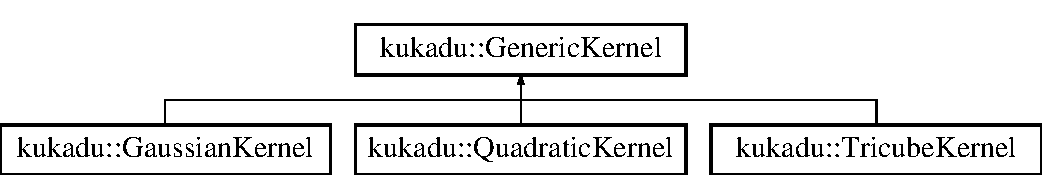
\includegraphics[height=2.000000cm]{classkukadu_1_1GenericKernel}
\end{center}
\end{figure}
\subsection*{Public Member Functions}
\begin{DoxyCompactItemize}
\item 
\hypertarget{classkukadu_1_1GenericKernel_a9392e79e7da5d8473ac9e42f74e8ef3e}{\hyperlink{classkukadu_1_1GenericKernel_a9392e79e7da5d8473ac9e42f74e8ef3e}{Generic\-Kernel} ()}\label{classkukadu_1_1GenericKernel_a9392e79e7da5d8473ac9e42f74e8ef3e}

\begin{DoxyCompactList}\small\item\em constructor \end{DoxyCompactList}\item 
virtual double \hyperlink{classkukadu_1_1GenericKernel_a802a15e8fb5f863e798c9114be976045}{evaluate\-Kernel} (arma\-::vec q1, arma\-::vec q2, void $\ast$kernel\-Param)=0
\begin{DoxyCompactList}\small\item\em computes kernel values with given vectors q1 and q2 and passes a not further specified kernel parameter that can be used by the kernel implementation \end{DoxyCompactList}\end{DoxyCompactItemize}


\subsection{Detailed Description}
Provides an interface for generic kernel functions. 

The \hyperlink{classkukadu_1_1GenericKernel}{Generic\-Kernel} class is used by the \hyperlink{classkukadu_1_1KernelRegressor}{Kernel\-Regressor}. Implementations of \hyperlink{classkukadu_1_1GenericKernel}{Generic\-Kernel} have to provide a certain kernel function, according to the kernel criteria. 

\subsection{Member Function Documentation}
\hypertarget{classkukadu_1_1GenericKernel_a802a15e8fb5f863e798c9114be976045}{\index{kukadu\-::\-Generic\-Kernel@{kukadu\-::\-Generic\-Kernel}!evaluate\-Kernel@{evaluate\-Kernel}}
\index{evaluate\-Kernel@{evaluate\-Kernel}!kukadu::GenericKernel@{kukadu\-::\-Generic\-Kernel}}
\subsubsection[{evaluate\-Kernel}]{\setlength{\rightskip}{0pt plus 5cm}virtual double kukadu\-::\-Generic\-Kernel\-::evaluate\-Kernel (
\begin{DoxyParamCaption}
\item[{arma\-::vec}]{q1, }
\item[{arma\-::vec}]{q2, }
\item[{void $\ast$}]{kernel\-Param}
\end{DoxyParamCaption}
)\hspace{0.3cm}{\ttfamily [pure virtual]}}}\label{classkukadu_1_1GenericKernel_a802a15e8fb5f863e798c9114be976045}


computes kernel values with given vectors q1 and q2 and passes a not further specified kernel parameter that can be used by the kernel implementation 


\begin{DoxyParams}{Parameters}
{\em q1} & vector q1 with K = K(d(q1, q2)) \\
\hline
{\em q2} & vector q2 with K = K(d(q1, q2)) \\
\hline
{\em kernel\-Param} & arbitrary kernel parameter \\
\hline
\end{DoxyParams}


Implemented in \hyperlink{classkukadu_1_1GaussianKernel_a11fec7aa4348f339008a454e268bf815}{kukadu\-::\-Gaussian\-Kernel}, \hyperlink{classkukadu_1_1QuadraticKernel_ac9a3385e7532ed38dcdcc0ee4acea035}{kukadu\-::\-Quadratic\-Kernel}, and \hyperlink{classkukadu_1_1TricubeKernel_a2c4053e0212bdfae0652c8bde2ae70df}{kukadu\-::\-Tricube\-Kernel}.



The documentation for this class was generated from the following files\-:\begin{DoxyCompactItemize}
\item 
/home/c7031109/iis\-\_\-robot\-\_\-sw/iis\-\_\-catkin\-\_\-ws/src/kukadu/include/kukadu/learning/regression/generickernel.\-hpp\item 
/home/c7031109/iis\-\_\-robot\-\_\-sw/iis\-\_\-catkin\-\_\-ws/src/kukadu/src/learning/generickernel.\-cpp\end{DoxyCompactItemize}

\hypertarget{classkukadu_1_1Gnuplot}{\section{kukadu\-:\-:Gnuplot Class Reference}
\label{classkukadu_1_1Gnuplot}\index{kukadu\-::\-Gnuplot@{kukadu\-::\-Gnuplot}}
}
\subsection*{Public Member Functions}
\begin{DoxyCompactItemize}
\item 
bool \hyperlink{classkukadu_1_1Gnuplot_a04d7a36bbe70dcb878a1ae5d8299d012}{set\-\_\-\-G\-N\-U\-Plot\-Path} (const std\-::string \&path)
\begin{DoxyCompactList}\small\item\em optional function\-: set \hyperlink{classkukadu_1_1Gnuplot}{Gnuplot} path manual attention\-: for windows\-: path with slash '/' not backslash '\textbackslash{}' \end{DoxyCompactList}\item 
void \hyperlink{classkukadu_1_1Gnuplot_aecc02fa13c09680a010e50331d50804c}{set\-\_\-terminal\-\_\-std} (const std\-::string \&type)
\item 
\hypertarget{classkukadu_1_1Gnuplot_afb20839c235bdf281f61a7c8e1ea8de9}{\hyperlink{classkukadu_1_1Gnuplot_afb20839c235bdf281f61a7c8e1ea8de9}{Gnuplot} (const std\-::string \&style=\char`\"{}lines lw 3\char`\"{})}\label{classkukadu_1_1Gnuplot_afb20839c235bdf281f61a7c8e1ea8de9}

\begin{DoxyCompactList}\small\item\em set a style during construction \end{DoxyCompactList}\item 
\hypertarget{classkukadu_1_1Gnuplot_a116918cb455b18e367cfcd34dfe2ecab}{\hyperlink{classkukadu_1_1Gnuplot_a116918cb455b18e367cfcd34dfe2ecab}{Gnuplot} (const std\-::vector$<$ double $>$ \&x, const std\-::string \&title=\char`\"{}\char`\"{}, const std\-::string \&style=\char`\"{}lines lw 3\char`\"{}, const std\-::string \&labelx=\char`\"{}x\char`\"{}, const std\-::string \&labely=\char`\"{}y\char`\"{})}\label{classkukadu_1_1Gnuplot_a116918cb455b18e367cfcd34dfe2ecab}

\begin{DoxyCompactList}\small\item\em plot a single std\-::vector at one go \end{DoxyCompactList}\item 
\hypertarget{classkukadu_1_1Gnuplot_a78963c977dfcc32904344da61d35e57a}{\hyperlink{classkukadu_1_1Gnuplot_a78963c977dfcc32904344da61d35e57a}{Gnuplot} (const std\-::vector$<$ double $>$ \&x, const std\-::vector$<$ double $>$ \&y, const std\-::string \&title=\char`\"{}\char`\"{}, const std\-::string \&style=\char`\"{}lines lw 3\char`\"{}, const std\-::string \&labelx=\char`\"{}x\char`\"{}, const std\-::string \&labely=\char`\"{}y\char`\"{})}\label{classkukadu_1_1Gnuplot_a78963c977dfcc32904344da61d35e57a}

\begin{DoxyCompactList}\small\item\em plot pairs std\-::vector at one go \end{DoxyCompactList}\item 
\hypertarget{classkukadu_1_1Gnuplot_a871b56fac856507973efb00861f7cd06}{\hyperlink{classkukadu_1_1Gnuplot_a871b56fac856507973efb00861f7cd06}{Gnuplot} (const std\-::vector$<$ double $>$ \&x, const std\-::vector$<$ double $>$ \&y, const std\-::vector$<$ double $>$ \&z, const std\-::string \&title=\char`\"{}\char`\"{}, const std\-::string \&style=\char`\"{}lines lw 3\char`\"{}, const std\-::string \&labelx=\char`\"{}x\char`\"{}, const std\-::string \&labely=\char`\"{}y\char`\"{}, const std\-::string \&labelz=\char`\"{}z\char`\"{})}\label{classkukadu_1_1Gnuplot_a871b56fac856507973efb00861f7cd06}

\begin{DoxyCompactList}\small\item\em plot triples std\-::vector at one go \end{DoxyCompactList}\item 
\hypertarget{classkukadu_1_1Gnuplot_a512e0f34eacae8a6a819b0b74fab029b}{\hyperlink{classkukadu_1_1Gnuplot_a512e0f34eacae8a6a819b0b74fab029b}{$\sim$\-Gnuplot} ()}\label{classkukadu_1_1Gnuplot_a512e0f34eacae8a6a819b0b74fab029b}

\begin{DoxyCompactList}\small\item\em destructor\-: needed to delete temporary files \end{DoxyCompactList}\item 
\hypertarget{classkukadu_1_1Gnuplot_a02945efc7719ceb26b97bdee6dfa0c76}{\hyperlink{classkukadu_1_1Gnuplot}{Gnuplot} \& \hyperlink{classkukadu_1_1Gnuplot_a02945efc7719ceb26b97bdee6dfa0c76}{cmd} (const std\-::string \&cmdstr)}\label{classkukadu_1_1Gnuplot_a02945efc7719ceb26b97bdee6dfa0c76}

\begin{DoxyCompactList}\small\item\em send a command to gnuplot \end{DoxyCompactList}\item 
\hyperlink{classkukadu_1_1Gnuplot}{Gnuplot} \& \hyperlink{classkukadu_1_1Gnuplot_a76d956598dab9d160127acf2c7d06e1f}{operator$<$$<$} (const std\-::string \&cmdstr)
\begin{DoxyCompactList}\small\item\em Sends a command to an active gnuplot session, identical to \hyperlink{classkukadu_1_1Gnuplot_a02945efc7719ceb26b97bdee6dfa0c76}{cmd()} send a command to gnuplot using the $<$$<$ operator. \end{DoxyCompactList}\item 
\hypertarget{classkukadu_1_1Gnuplot_a88c750479a441fe5e0113e7f795d6f42}{\hyperlink{classkukadu_1_1Gnuplot}{Gnuplot} \& \hyperlink{classkukadu_1_1Gnuplot_a88c750479a441fe5e0113e7f795d6f42}{showonscreen} ()}\label{classkukadu_1_1Gnuplot_a88c750479a441fe5e0113e7f795d6f42}

\begin{DoxyCompactList}\small\item\em sets terminal type to terminal\-\_\-std \end{DoxyCompactList}\item 
\hypertarget{classkukadu_1_1Gnuplot_ae6857197036b0739d792b5aa3833c673}{\hyperlink{classkukadu_1_1Gnuplot}{Gnuplot} \& \hyperlink{classkukadu_1_1Gnuplot_ae6857197036b0739d792b5aa3833c673}{savetops} (const std\-::string \&filename=\char`\"{}gnuplot\-\_\-output\char`\"{})}\label{classkukadu_1_1Gnuplot_ae6857197036b0739d792b5aa3833c673}

\begin{DoxyCompactList}\small\item\em saves a gnuplot session to a postscript file, filename without extension \end{DoxyCompactList}\item 
\hyperlink{classkukadu_1_1Gnuplot}{Gnuplot} \& \hyperlink{classkukadu_1_1Gnuplot_a168775b6cf04b25a621886d2f0f85806}{set\-\_\-style} (const std\-::string \&stylestr=\char`\"{}points\char`\"{})
\item 
\hyperlink{classkukadu_1_1Gnuplot}{Gnuplot} \& \hyperlink{classkukadu_1_1Gnuplot_a8b8849a77a1c674c30e4e5f8d59f8308}{set\-\_\-smooth} (const std\-::string \&stylestr=\char`\"{}csplines\char`\"{})
\item 
\hyperlink{classkukadu_1_1Gnuplot}{Gnuplot} \& \hyperlink{classkukadu_1_1Gnuplot_abbebd88fffd2654ff192d6222f4d8e65}{unset\-\_\-smooth} ()
\begin{DoxyCompactList}\small\item\em unset smooth attention\-: smooth is not set by default \end{DoxyCompactList}\item 
\hypertarget{classkukadu_1_1Gnuplot_ab1033881b0494423cd292c5084bf3925}{\hyperlink{classkukadu_1_1Gnuplot}{Gnuplot} \& \hyperlink{classkukadu_1_1Gnuplot_ab1033881b0494423cd292c5084bf3925}{set\-\_\-pointsize} (const double pointsize=1.\-0)}\label{classkukadu_1_1Gnuplot_ab1033881b0494423cd292c5084bf3925}

\begin{DoxyCompactList}\small\item\em scales the size of the points used in plots \end{DoxyCompactList}\item 
\hypertarget{classkukadu_1_1Gnuplot_aebcefffa35cefd5e4e0cffab0f3b5a6a}{\hyperlink{classkukadu_1_1Gnuplot}{Gnuplot} \& \hyperlink{classkukadu_1_1Gnuplot_aebcefffa35cefd5e4e0cffab0f3b5a6a}{set\-\_\-grid} ()}\label{classkukadu_1_1Gnuplot_aebcefffa35cefd5e4e0cffab0f3b5a6a}

\begin{DoxyCompactList}\small\item\em turns grid on/off \end{DoxyCompactList}\item 
\hypertarget{classkukadu_1_1Gnuplot_a58316e0929ce39f1a50aefd528ba835e}{\hyperlink{classkukadu_1_1Gnuplot}{Gnuplot} \& \hyperlink{classkukadu_1_1Gnuplot_a58316e0929ce39f1a50aefd528ba835e}{unset\-\_\-grid} ()}\label{classkukadu_1_1Gnuplot_a58316e0929ce39f1a50aefd528ba835e}

\begin{DoxyCompactList}\small\item\em grid is not set by default \end{DoxyCompactList}\item 
\hyperlink{classkukadu_1_1Gnuplot}{Gnuplot} \& \hyperlink{classkukadu_1_1Gnuplot_aab85e8b17756b471d3c800be4aab9cff}{set\-\_\-multiplot} ()
\item 
\hyperlink{classkukadu_1_1Gnuplot}{Gnuplot} \& \hyperlink{classkukadu_1_1Gnuplot_a91600bc5fa98295f48440bb211ba89db}{unset\-\_\-multiplot} ()
\item 
\hypertarget{classkukadu_1_1Gnuplot_aed34438f8adfdd17b5b529e77eca3dd8}{\hyperlink{classkukadu_1_1Gnuplot}{Gnuplot} \& \hyperlink{classkukadu_1_1Gnuplot_aed34438f8adfdd17b5b529e77eca3dd8}{set\-\_\-samples} (const int samples=100)}\label{classkukadu_1_1Gnuplot_aed34438f8adfdd17b5b529e77eca3dd8}

\begin{DoxyCompactList}\small\item\em set sampling rate of functions, or for interpolating data \end{DoxyCompactList}\item 
\hypertarget{classkukadu_1_1Gnuplot_ae915b506a6ad7667635b1c8f2d41365e}{\hyperlink{classkukadu_1_1Gnuplot}{Gnuplot} \& \hyperlink{classkukadu_1_1Gnuplot_ae915b506a6ad7667635b1c8f2d41365e}{set\-\_\-isosamples} (const int isolines=10)}\label{classkukadu_1_1Gnuplot_ae915b506a6ad7667635b1c8f2d41365e}

\begin{DoxyCompactList}\small\item\em set isoline density (grid) for plotting functions as surfaces (for 3d plots) \end{DoxyCompactList}\item 
\hyperlink{classkukadu_1_1Gnuplot}{Gnuplot} \& \hyperlink{classkukadu_1_1Gnuplot_ac6aa969947a3e5ad968726b58d839d0a}{set\-\_\-hidden3d} ()
\item 
\hyperlink{classkukadu_1_1Gnuplot}{Gnuplot} \& \hyperlink{classkukadu_1_1Gnuplot_a4e93a0f9c069b953a70502765d31dc1e}{unset\-\_\-hidden3d} ()
\item 
\hyperlink{classkukadu_1_1Gnuplot}{Gnuplot} \& \hyperlink{classkukadu_1_1Gnuplot_a6666c2286bcd0f8fea294b94a6c8545c}{set\-\_\-contour} (const std\-::string \&position=\char`\"{}base\char`\"{})
\item 
\hyperlink{classkukadu_1_1Gnuplot}{Gnuplot} \& \hyperlink{classkukadu_1_1Gnuplot_a6fe8c0d459872698c3531c50cf57be88}{unset\-\_\-contour} ()
\item 
\hyperlink{classkukadu_1_1Gnuplot}{Gnuplot} \& \hyperlink{classkukadu_1_1Gnuplot_a2b1dba26cececc7cb0c0c3d6c6345c18}{set\-\_\-surface} ()
\item 
\hyperlink{classkukadu_1_1Gnuplot}{Gnuplot} \& \hyperlink{classkukadu_1_1Gnuplot_a23283eaf224fede9a5a9378f678226a1}{unset\-\_\-surface} ()
\item 
\hyperlink{classkukadu_1_1Gnuplot}{Gnuplot} \& \hyperlink{classkukadu_1_1Gnuplot_aca9ce23dbc33bd29ff563c23a29e47ae}{set\-\_\-legend} (const std\-::string \&position=\char`\"{}default\char`\"{})
\item 
\hyperlink{classkukadu_1_1Gnuplot}{Gnuplot} \& \hyperlink{classkukadu_1_1Gnuplot_a5c8dab8e316a7d9b316d45f715ff0859}{unset\-\_\-legend} ()
\begin{DoxyCompactList}\small\item\em Switches legend off attention\-:legend is set by default. \end{DoxyCompactList}\item 
\hyperlink{classkukadu_1_1Gnuplot}{Gnuplot} \& \hyperlink{classkukadu_1_1Gnuplot_a1f0757bd29d5e3bee4e23be95951bc13}{set\-\_\-title} (const std\-::string \&title=\char`\"{}\char`\"{})
\begin{DoxyCompactList}\small\item\em sets and clears the title of a gnuplot session \end{DoxyCompactList}\item 
\hyperlink{classkukadu_1_1Gnuplot}{Gnuplot} \& \hyperlink{classkukadu_1_1Gnuplot_a5fc9e87f3c624fbff79a960c66a16bd1}{unset\-\_\-title} ()
\begin{DoxyCompactList}\small\item\em Clears the title of a gnuplot session The title is not set by default. \end{DoxyCompactList}\item 
\hypertarget{classkukadu_1_1Gnuplot_abee1cfd744420fd989db8092acedcc93}{\hyperlink{classkukadu_1_1Gnuplot}{Gnuplot} \& \hyperlink{classkukadu_1_1Gnuplot_abee1cfd744420fd989db8092acedcc93}{set\-\_\-ylabel} (const std\-::string \&label=\char`\"{}x\char`\"{})}\label{classkukadu_1_1Gnuplot_abee1cfd744420fd989db8092acedcc93}

\begin{DoxyCompactList}\small\item\em set x axis label \end{DoxyCompactList}\item 
\hypertarget{classkukadu_1_1Gnuplot_a48b3c2b23f740375b73d27d1906968d0}{\hyperlink{classkukadu_1_1Gnuplot}{Gnuplot} \& \hyperlink{classkukadu_1_1Gnuplot_a48b3c2b23f740375b73d27d1906968d0}{set\-\_\-xlabel} (const std\-::string \&label=\char`\"{}y\char`\"{})}\label{classkukadu_1_1Gnuplot_a48b3c2b23f740375b73d27d1906968d0}

\begin{DoxyCompactList}\small\item\em set y axis label \end{DoxyCompactList}\item 
\hypertarget{classkukadu_1_1Gnuplot_a439a74f49c171b12df1a941a39b3e8c1}{\hyperlink{classkukadu_1_1Gnuplot}{Gnuplot} \& \hyperlink{classkukadu_1_1Gnuplot_a439a74f49c171b12df1a941a39b3e8c1}{set\-\_\-zlabel} (const std\-::string \&label=\char`\"{}z\char`\"{})}\label{classkukadu_1_1Gnuplot_a439a74f49c171b12df1a941a39b3e8c1}

\begin{DoxyCompactList}\small\item\em set z axis label \end{DoxyCompactList}\item 
\hypertarget{classkukadu_1_1Gnuplot_a1e27f156415728196a52946e304f5d1e}{\hyperlink{classkukadu_1_1Gnuplot}{Gnuplot} \& \hyperlink{classkukadu_1_1Gnuplot_a1e27f156415728196a52946e304f5d1e}{set\-\_\-xrange} (const double i\-From, const double i\-To)}\label{classkukadu_1_1Gnuplot_a1e27f156415728196a52946e304f5d1e}

\begin{DoxyCompactList}\small\item\em set axis -\/ ranges \end{DoxyCompactList}\item 
\hypertarget{classkukadu_1_1Gnuplot_a5b27c86aa6c5505aa9b7f65958f1da26}{\hyperlink{classkukadu_1_1Gnuplot}{Gnuplot} \& \hyperlink{classkukadu_1_1Gnuplot_a5b27c86aa6c5505aa9b7f65958f1da26}{set\-\_\-yrange} (const double i\-From, const double i\-To)}\label{classkukadu_1_1Gnuplot_a5b27c86aa6c5505aa9b7f65958f1da26}

\begin{DoxyCompactList}\small\item\em set y-\/axis -\/ ranges \end{DoxyCompactList}\item 
\hypertarget{classkukadu_1_1Gnuplot_a719ea05d40c1cdd23f6844a494064720}{\hyperlink{classkukadu_1_1Gnuplot}{Gnuplot} \& \hyperlink{classkukadu_1_1Gnuplot_a719ea05d40c1cdd23f6844a494064720}{set\-\_\-zrange} (const double i\-From, const double i\-To)}\label{classkukadu_1_1Gnuplot_a719ea05d40c1cdd23f6844a494064720}

\begin{DoxyCompactList}\small\item\em set z-\/axis -\/ ranges \end{DoxyCompactList}\item 
\hyperlink{classkukadu_1_1Gnuplot}{Gnuplot} \& \hyperlink{classkukadu_1_1Gnuplot_ad895bac1da923236a2bbbddf13df4f5b}{set\-\_\-xautoscale} ()
\item 
\hyperlink{classkukadu_1_1Gnuplot}{Gnuplot} \& \hyperlink{classkukadu_1_1Gnuplot_aa5c079210584a06fa50ae99f5fe2d00d}{set\-\_\-yautoscale} ()
\item 
\hyperlink{classkukadu_1_1Gnuplot}{Gnuplot} \& \hyperlink{classkukadu_1_1Gnuplot_a24266265b9d32e8991d1ac053dbc58c5}{set\-\_\-zautoscale} ()
\item 
\hypertarget{classkukadu_1_1Gnuplot_a11893bdae68ab25f8ecb95818ca65395}{\hyperlink{classkukadu_1_1Gnuplot}{Gnuplot} \& \hyperlink{classkukadu_1_1Gnuplot_a11893bdae68ab25f8ecb95818ca65395}{set\-\_\-xlogscale} (const double base=10)}\label{classkukadu_1_1Gnuplot_a11893bdae68ab25f8ecb95818ca65395}

\begin{DoxyCompactList}\small\item\em turns on/off log scaling for the specified xaxis (logscale is not set by default) \end{DoxyCompactList}\item 
\hypertarget{classkukadu_1_1Gnuplot_a83bdceeb4e068075caf98b030ef9372f}{\hyperlink{classkukadu_1_1Gnuplot}{Gnuplot} \& \hyperlink{classkukadu_1_1Gnuplot_a83bdceeb4e068075caf98b030ef9372f}{set\-\_\-ylogscale} (const double base=10)}\label{classkukadu_1_1Gnuplot_a83bdceeb4e068075caf98b030ef9372f}

\begin{DoxyCompactList}\small\item\em turns on/off log scaling for the specified yaxis (logscale is not set by default) \end{DoxyCompactList}\item 
\hypertarget{classkukadu_1_1Gnuplot_aaeecd89ae7aabf9fb304f60965198588}{\hyperlink{classkukadu_1_1Gnuplot}{Gnuplot} \& \hyperlink{classkukadu_1_1Gnuplot_aaeecd89ae7aabf9fb304f60965198588}{set\-\_\-zlogscale} (const double base=10)}\label{classkukadu_1_1Gnuplot_aaeecd89ae7aabf9fb304f60965198588}

\begin{DoxyCompactList}\small\item\em turns on/off log scaling for the specified zaxis (logscale is not set by default) \end{DoxyCompactList}\item 
\hyperlink{classkukadu_1_1Gnuplot}{Gnuplot} \& \hyperlink{classkukadu_1_1Gnuplot_a8d4ff3b840757c7d7e248aa2932dfd9e}{unset\-\_\-xlogscale} ()
\item 
\hyperlink{classkukadu_1_1Gnuplot}{Gnuplot} \& \hyperlink{classkukadu_1_1Gnuplot_ab4faf2a5d5572733967ef00b03937a98}{unset\-\_\-ylogscale} ()
\item 
\hyperlink{classkukadu_1_1Gnuplot}{Gnuplot} \& \hyperlink{classkukadu_1_1Gnuplot_a2bccf59dc2f3dc853d45e6f0ebbc33e2}{unset\-\_\-zlogscale} ()
\item 
\hypertarget{classkukadu_1_1Gnuplot_ab1eeecc6cca9d87af3be7af4e37ab1c0}{\hyperlink{classkukadu_1_1Gnuplot}{Gnuplot} \& \hyperlink{classkukadu_1_1Gnuplot_ab1eeecc6cca9d87af3be7af4e37ab1c0}{set\-\_\-cbrange} (const double i\-From, const double i\-To)}\label{classkukadu_1_1Gnuplot_ab1eeecc6cca9d87af3be7af4e37ab1c0}

\begin{DoxyCompactList}\small\item\em set palette range (autoscale by default) \end{DoxyCompactList}\item 
\hyperlink{classkukadu_1_1Gnuplot}{Gnuplot} \& \hyperlink{classkukadu_1_1Gnuplot_a6f7bb713dd84b3ad5a737f7005411bfc}{plotfile\-\_\-x} (const std\-::string \&filename, const unsigned int column=1, const std\-::string \&title=\char`\"{}\char`\"{})
\item 
{\footnotesize template$<$typename X $>$ }\\\hyperlink{classkukadu_1_1Gnuplot}{Gnuplot} \& \hyperlink{classkukadu_1_1Gnuplot_af942480ea37a33cbd5bef00e8592404d}{plot\-\_\-x} (const X \&x, const std\-::string \&title=\char`\"{}\char`\"{})
\begin{DoxyCompactList}\small\item\em from std\-::vector \end{DoxyCompactList}\item 
\hyperlink{classkukadu_1_1Gnuplot}{Gnuplot} \& \hyperlink{classkukadu_1_1Gnuplot_a69a964c20551ba369846d10c74e53d51}{plotfile\-\_\-xy} (const std\-::string \&filename, const unsigned int column\-\_\-x=1, const unsigned int column\-\_\-y=2, const std\-::string \&title=\char`\"{}\char`\"{})
\item 
{\footnotesize template$<$typename X , typename Y $>$ }\\\hyperlink{classkukadu_1_1Gnuplot}{Gnuplot} \& \hyperlink{classkukadu_1_1Gnuplot_ac80122ec909d18c1c1b22bd7c3570fb9}{plot\-\_\-xy} (const X \&x, const Y \&y, const std\-::string \&title=\char`\"{}\char`\"{})
\begin{DoxyCompactList}\small\item\em from data \end{DoxyCompactList}\item 
\hyperlink{classkukadu_1_1Gnuplot}{Gnuplot} \& \hyperlink{classkukadu_1_1Gnuplot_a78fb33f6b8f7c169bad61f7767b4452f}{plotfile\-\_\-xy\-\_\-err} (const std\-::string \&filename, const unsigned int column\-\_\-x=1, const unsigned int column\-\_\-y=2, const unsigned int column\-\_\-dy=3, const std\-::string \&title=\char`\"{}\char`\"{})
\item 
{\footnotesize template$<$typename X , typename Y , typename E $>$ }\\\hyperlink{classkukadu_1_1Gnuplot}{Gnuplot} \& \hyperlink{classkukadu_1_1Gnuplot_a4cc62bb2504de6635ed6b47cbaf02c1c}{plot\-\_\-xy\-\_\-err} (const X \&x, const Y \&y, const E \&dy, const std\-::string \&title=\char`\"{}\char`\"{})
\begin{DoxyCompactList}\small\item\em from data \end{DoxyCompactList}\item 
\hyperlink{classkukadu_1_1Gnuplot}{Gnuplot} \& \hyperlink{classkukadu_1_1Gnuplot_a03b4eec7a72bc05abfcdfd7bcd61513b}{plotfile\-\_\-xyz} (const std\-::string \&filename, const unsigned int column\-\_\-x=1, const unsigned int column\-\_\-y=2, const unsigned int column\-\_\-z=3, const std\-::string \&title=\char`\"{}\char`\"{})
\item 
\hypertarget{classkukadu_1_1Gnuplot_ac3e5d63b5a9729d5e609e45abc65520f}{{\footnotesize template$<$typename X , typename Y , typename Z $>$ }\\\hyperlink{classkukadu_1_1Gnuplot}{Gnuplot} \& \hyperlink{classkukadu_1_1Gnuplot_ac3e5d63b5a9729d5e609e45abc65520f}{plot\-\_\-xyz} (const X \&x, const Y \&y, const Z \&z, const std\-::string \&title=\char`\"{}\char`\"{})}\label{classkukadu_1_1Gnuplot_ac3e5d63b5a9729d5e609e45abc65520f}

\begin{DoxyCompactList}\small\item\em from std\-::vector \end{DoxyCompactList}\item 
\hypertarget{classkukadu_1_1Gnuplot_aaddc220bf3a1726a962c801a1218b826}{\hyperlink{classkukadu_1_1Gnuplot}{Gnuplot} \& \hyperlink{classkukadu_1_1Gnuplot_aaddc220bf3a1726a962c801a1218b826}{plot\-\_\-slope} (const double a, const double b, const std\-::string \&title=\char`\"{}\char`\"{})}\label{classkukadu_1_1Gnuplot_aaddc220bf3a1726a962c801a1218b826}

\begin{DoxyCompactList}\small\item\em plot an equation of the form\-: y = ax + b, you supply a and b \end{DoxyCompactList}\item 
\hyperlink{classkukadu_1_1Gnuplot}{Gnuplot} \& \hyperlink{classkukadu_1_1Gnuplot_a96c92aa357fa26095bfeb7afcc1d7ae5}{plot\-\_\-equation} (const std\-::string \&equation, const std\-::string \&title=\char`\"{}\char`\"{})
\item 
\hyperlink{classkukadu_1_1Gnuplot}{Gnuplot} \& \hyperlink{classkukadu_1_1Gnuplot_a2500bea1234a30061b30cb66247d101e}{plot\-\_\-equation3d} (const std\-::string \&equation, const std\-::string \&title=\char`\"{}\char`\"{})
\item 
\hyperlink{classkukadu_1_1Gnuplot}{Gnuplot} \& \hyperlink{classkukadu_1_1Gnuplot_a00fa2629225493cef7be8e0263fb7fa4}{plot\-\_\-image} (const unsigned char $\ast$uc\-Pic\-Buf, const unsigned int i\-Width, const unsigned int i\-Height, const std\-::string \&title=\char`\"{}\char`\"{})
\begin{DoxyCompactList}\small\item\em plot image \end{DoxyCompactList}\item 
\hyperlink{classkukadu_1_1Gnuplot}{Gnuplot} \& \hyperlink{classkukadu_1_1Gnuplot_a775739d7e45f805b8e8d6629a7fc1e6c}{replot} (void)
\begin{DoxyCompactList}\small\item\em replot repeats the last plot or splot command. this can be useful for viewing a plot with different set options, or when generating the same plot for several devices (showonscreen, savetops) \end{DoxyCompactList}\item 
\hypertarget{classkukadu_1_1Gnuplot_a8437ccf75a256391bc8727c72af71ba7}{\hyperlink{classkukadu_1_1Gnuplot}{Gnuplot} \& \hyperlink{classkukadu_1_1Gnuplot_a8437ccf75a256391bc8727c72af71ba7}{reset\-\_\-plot} ()}\label{classkukadu_1_1Gnuplot_a8437ccf75a256391bc8727c72af71ba7}

\begin{DoxyCompactList}\small\item\em resets a gnuplot session (next plot will erase previous ones) \end{DoxyCompactList}\item 
\hypertarget{classkukadu_1_1Gnuplot_a90fcd1025b2bc89e5d1f1d3c0ac4121e}{\hyperlink{classkukadu_1_1Gnuplot}{Gnuplot} \& \hyperlink{classkukadu_1_1Gnuplot_a90fcd1025b2bc89e5d1f1d3c0ac4121e}{reset\-\_\-all} ()}\label{classkukadu_1_1Gnuplot_a90fcd1025b2bc89e5d1f1d3c0ac4121e}

\begin{DoxyCompactList}\small\item\em resets a gnuplot session and sets all variables to default \end{DoxyCompactList}\item 
\hypertarget{classkukadu_1_1Gnuplot_ae0d9d829d071346b0d137ea5167417a0}{void \hyperlink{classkukadu_1_1Gnuplot_ae0d9d829d071346b0d137ea5167417a0}{remove\-\_\-tmpfiles} ()}\label{classkukadu_1_1Gnuplot_ae0d9d829d071346b0d137ea5167417a0}

\begin{DoxyCompactList}\small\item\em deletes temporary files \end{DoxyCompactList}\item 
bool \hyperlink{classkukadu_1_1Gnuplot_af51379284d1d3b6b2e1a51106a81788b}{is\-\_\-valid} ()
\begin{DoxyCompactList}\small\item\em Is the gnuplot session valid ?? \end{DoxyCompactList}\end{DoxyCompactItemize}


\subsection{Member Function Documentation}
\hypertarget{classkukadu_1_1Gnuplot_af51379284d1d3b6b2e1a51106a81788b}{\index{kukadu\-::\-Gnuplot@{kukadu\-::\-Gnuplot}!is\-\_\-valid@{is\-\_\-valid}}
\index{is\-\_\-valid@{is\-\_\-valid}!kukadu::Gnuplot@{kukadu\-::\-Gnuplot}}
\subsubsection[{is\-\_\-valid}]{\setlength{\rightskip}{0pt plus 5cm}bool kukadu\-::\-Gnuplot\-::is\-\_\-valid (
\begin{DoxyParamCaption}
{}
\end{DoxyParamCaption}
)\hspace{0.3cm}{\ttfamily [inline]}}}\label{classkukadu_1_1Gnuplot_af51379284d1d3b6b2e1a51106a81788b}


Is the gnuplot session valid ?? 


\begin{DoxyParams}{Parameters}
{\em \&mdash;} & \\
\hline
\end{DoxyParams}
\begin{DoxyReturn}{Returns}
true if valid, false if not 
\end{DoxyReturn}
\hypertarget{classkukadu_1_1Gnuplot_a76d956598dab9d160127acf2c7d06e1f}{\index{kukadu\-::\-Gnuplot@{kukadu\-::\-Gnuplot}!operator$<$$<$@{operator$<$$<$}}
\index{operator$<$$<$@{operator$<$$<$}!kukadu::Gnuplot@{kukadu\-::\-Gnuplot}}
\subsubsection[{operator$<$$<$}]{\setlength{\rightskip}{0pt plus 5cm}{\bf Gnuplot}\& kukadu\-::\-Gnuplot\-::operator$<$$<$ (
\begin{DoxyParamCaption}
\item[{const std\-::string \&}]{cmdstr}
\end{DoxyParamCaption}
)\hspace{0.3cm}{\ttfamily [inline]}}}\label{classkukadu_1_1Gnuplot_a76d956598dab9d160127acf2c7d06e1f}


Sends a command to an active gnuplot session, identical to \hyperlink{classkukadu_1_1Gnuplot_a02945efc7719ceb26b97bdee6dfa0c76}{cmd()} send a command to gnuplot using the $<$$<$ operator. 


\begin{DoxyParams}{Parameters}
{\em cmdstr} & --$>$ the command string\\
\hline
\end{DoxyParams}
\begin{DoxyReturn}{Returns}
$<$-- a reference to the gnuplot object 
\end{DoxyReturn}
\hypertarget{classkukadu_1_1Gnuplot_a96c92aa357fa26095bfeb7afcc1d7ae5}{\index{kukadu\-::\-Gnuplot@{kukadu\-::\-Gnuplot}!plot\-\_\-equation@{plot\-\_\-equation}}
\index{plot\-\_\-equation@{plot\-\_\-equation}!kukadu::Gnuplot@{kukadu\-::\-Gnuplot}}
\subsubsection[{plot\-\_\-equation}]{\setlength{\rightskip}{0pt plus 5cm}{\bf Gnuplot} \& kukadu\-::\-Gnuplot\-::plot\-\_\-equation (
\begin{DoxyParamCaption}
\item[{const std\-::string \&}]{equation, }
\item[{const std\-::string \&}]{title = {\ttfamily \char`\"{}\char`\"{}}}
\end{DoxyParamCaption}
)}}\label{classkukadu_1_1Gnuplot_a96c92aa357fa26095bfeb7afcc1d7ae5}
plot an equation supplied as a std\-::string y=f(x), write only the function f(x) not y= the independent variable has to be x binary operators\-: $\ast$$\ast$ exponentiation, $\ast$ multiply, / divide, + add, -\/ substract, \% modulo unary operators\-: -\/ minus, ! factorial elementary functions\-: rand(x), abs(x), sgn(x), ceil(x), floor(x), int(x), imag(x), real(x), arg(x), sqrt(x), exp(x), log(x), log10(x), sin(x), cos(x), tan(x), asin(x), acos(x), atan(x), atan2(y,x), sinh(x), cosh(x), tanh(x), asinh(x), acosh(x), atanh(x) special functions\-: erf(x), erfc(x), inverf(x), gamma(x), igamma(a,x), lgamma(x), ibeta(p,q,x), besj0(x), besj1(x), besy0(x), besy1(x), lambertw(x) statistical fuctions\-: norm(x), invnorm(x) \hypertarget{classkukadu_1_1Gnuplot_a2500bea1234a30061b30cb66247d101e}{\index{kukadu\-::\-Gnuplot@{kukadu\-::\-Gnuplot}!plot\-\_\-equation3d@{plot\-\_\-equation3d}}
\index{plot\-\_\-equation3d@{plot\-\_\-equation3d}!kukadu::Gnuplot@{kukadu\-::\-Gnuplot}}
\subsubsection[{plot\-\_\-equation3d}]{\setlength{\rightskip}{0pt plus 5cm}{\bf Gnuplot} \& kukadu\-::\-Gnuplot\-::plot\-\_\-equation3d (
\begin{DoxyParamCaption}
\item[{const std\-::string \&}]{equation, }
\item[{const std\-::string \&}]{title = {\ttfamily \char`\"{}\char`\"{}}}
\end{DoxyParamCaption}
)}}\label{classkukadu_1_1Gnuplot_a2500bea1234a30061b30cb66247d101e}
plot an equation supplied as a std\-::string z=f(x,y), write only the function f(x,y) not z= the independent variables have to be x and y \hypertarget{classkukadu_1_1Gnuplot_a00fa2629225493cef7be8e0263fb7fa4}{\index{kukadu\-::\-Gnuplot@{kukadu\-::\-Gnuplot}!plot\-\_\-image@{plot\-\_\-image}}
\index{plot\-\_\-image@{plot\-\_\-image}!kukadu::Gnuplot@{kukadu\-::\-Gnuplot}}
\subsubsection[{plot\-\_\-image}]{\setlength{\rightskip}{0pt plus 5cm}{\bf Gnuplot} \& kukadu\-::\-Gnuplot\-::plot\-\_\-image (
\begin{DoxyParamCaption}
\item[{const unsigned char $\ast$}]{uc\-Pic\-Buf, }
\item[{const unsigned int}]{i\-Width, }
\item[{const unsigned int}]{i\-Height, }
\item[{const std\-::string \&}]{title = {\ttfamily \char`\"{}\char`\"{}}}
\end{DoxyParamCaption}
)}}\label{classkukadu_1_1Gnuplot_a00fa2629225493cef7be8e0263fb7fa4}


plot image 


\begin{DoxyItemize}
\item note that this function is not valid for versions of G\-N\-U\-Plot below 4.\-2 
\end{DoxyItemize}\hypertarget{classkukadu_1_1Gnuplot_af942480ea37a33cbd5bef00e8592404d}{\index{kukadu\-::\-Gnuplot@{kukadu\-::\-Gnuplot}!plot\-\_\-x@{plot\-\_\-x}}
\index{plot\-\_\-x@{plot\-\_\-x}!kukadu::Gnuplot@{kukadu\-::\-Gnuplot}}
\subsubsection[{plot\-\_\-x}]{\setlength{\rightskip}{0pt plus 5cm}template$<$typename X $>$ {\bf Gnuplot} \& kukadu\-::\-Gnuplot\-::plot\-\_\-x (
\begin{DoxyParamCaption}
\item[{const X \&}]{x, }
\item[{const std\-::string \&}]{title = {\ttfamily \char`\"{}\char`\"{}}}
\end{DoxyParamCaption}
)}}\label{classkukadu_1_1Gnuplot_af942480ea37a33cbd5bef00e8592404d}


from std\-::vector 

Plots a 2d graph from a list of doubles\-: x. \hypertarget{classkukadu_1_1Gnuplot_ac80122ec909d18c1c1b22bd7c3570fb9}{\index{kukadu\-::\-Gnuplot@{kukadu\-::\-Gnuplot}!plot\-\_\-xy@{plot\-\_\-xy}}
\index{plot\-\_\-xy@{plot\-\_\-xy}!kukadu::Gnuplot@{kukadu\-::\-Gnuplot}}
\subsubsection[{plot\-\_\-xy}]{\setlength{\rightskip}{0pt plus 5cm}template$<$typename X , typename Y $>$ {\bf Gnuplot} \& kukadu\-::\-Gnuplot\-::plot\-\_\-xy (
\begin{DoxyParamCaption}
\item[{const X \&}]{x, }
\item[{const Y \&}]{y, }
\item[{const std\-::string \&}]{title = {\ttfamily \char`\"{}\char`\"{}}}
\end{DoxyParamCaption}
)}}\label{classkukadu_1_1Gnuplot_ac80122ec909d18c1c1b22bd7c3570fb9}


from data 

Plots a 2d graph from a list of doubles\-: x y. \hypertarget{classkukadu_1_1Gnuplot_a4cc62bb2504de6635ed6b47cbaf02c1c}{\index{kukadu\-::\-Gnuplot@{kukadu\-::\-Gnuplot}!plot\-\_\-xy\-\_\-err@{plot\-\_\-xy\-\_\-err}}
\index{plot\-\_\-xy\-\_\-err@{plot\-\_\-xy\-\_\-err}!kukadu::Gnuplot@{kukadu\-::\-Gnuplot}}
\subsubsection[{plot\-\_\-xy\-\_\-err}]{\setlength{\rightskip}{0pt plus 5cm}template$<$typename X , typename Y , typename E $>$ {\bf Gnuplot} \& kukadu\-::\-Gnuplot\-::plot\-\_\-xy\-\_\-err (
\begin{DoxyParamCaption}
\item[{const X \&}]{x, }
\item[{const Y \&}]{y, }
\item[{const E \&}]{dy, }
\item[{const std\-::string \&}]{title = {\ttfamily \char`\"{}\char`\"{}}}
\end{DoxyParamCaption}
)}}\label{classkukadu_1_1Gnuplot_a4cc62bb2504de6635ed6b47cbaf02c1c}


from data 





plot x,y pairs with dy errorbars \hypertarget{classkukadu_1_1Gnuplot_a6f7bb713dd84b3ad5a737f7005411bfc}{\index{kukadu\-::\-Gnuplot@{kukadu\-::\-Gnuplot}!plotfile\-\_\-x@{plotfile\-\_\-x}}
\index{plotfile\-\_\-x@{plotfile\-\_\-x}!kukadu::Gnuplot@{kukadu\-::\-Gnuplot}}
\subsubsection[{plotfile\-\_\-x}]{\setlength{\rightskip}{0pt plus 5cm}{\bf Gnuplot} \& kukadu\-::\-Gnuplot\-::plotfile\-\_\-x (
\begin{DoxyParamCaption}
\item[{const std\-::string \&}]{filename, }
\item[{const unsigned int}]{column = {\ttfamily 1}, }
\item[{const std\-::string \&}]{title = {\ttfamily \char`\"{}\char`\"{}}}
\end{DoxyParamCaption}
)}}\label{classkukadu_1_1Gnuplot_a6f7bb713dd84b3ad5a737f7005411bfc}
plot a single std\-::vector\-: x from file \hypertarget{classkukadu_1_1Gnuplot_a69a964c20551ba369846d10c74e53d51}{\index{kukadu\-::\-Gnuplot@{kukadu\-::\-Gnuplot}!plotfile\-\_\-xy@{plotfile\-\_\-xy}}
\index{plotfile\-\_\-xy@{plotfile\-\_\-xy}!kukadu::Gnuplot@{kukadu\-::\-Gnuplot}}
\subsubsection[{plotfile\-\_\-xy}]{\setlength{\rightskip}{0pt plus 5cm}{\bf Gnuplot} \& kukadu\-::\-Gnuplot\-::plotfile\-\_\-xy (
\begin{DoxyParamCaption}
\item[{const std\-::string \&}]{filename, }
\item[{const unsigned int}]{column\-\_\-x = {\ttfamily 1}, }
\item[{const unsigned int}]{column\-\_\-y = {\ttfamily 2}, }
\item[{const std\-::string \&}]{title = {\ttfamily \char`\"{}\char`\"{}}}
\end{DoxyParamCaption}
)}}\label{classkukadu_1_1Gnuplot_a69a964c20551ba369846d10c74e53d51}
plot x,y pairs\-: x y from file \hypertarget{classkukadu_1_1Gnuplot_a78fb33f6b8f7c169bad61f7767b4452f}{\index{kukadu\-::\-Gnuplot@{kukadu\-::\-Gnuplot}!plotfile\-\_\-xy\-\_\-err@{plotfile\-\_\-xy\-\_\-err}}
\index{plotfile\-\_\-xy\-\_\-err@{plotfile\-\_\-xy\-\_\-err}!kukadu::Gnuplot@{kukadu\-::\-Gnuplot}}
\subsubsection[{plotfile\-\_\-xy\-\_\-err}]{\setlength{\rightskip}{0pt plus 5cm}{\bf Gnuplot} \& kukadu\-::\-Gnuplot\-::plotfile\-\_\-xy\-\_\-err (
\begin{DoxyParamCaption}
\item[{const std\-::string \&}]{filename, }
\item[{const unsigned int}]{column\-\_\-x = {\ttfamily 1}, }
\item[{const unsigned int}]{column\-\_\-y = {\ttfamily 2}, }
\item[{const unsigned int}]{column\-\_\-dy = {\ttfamily 3}, }
\item[{const std\-::string \&}]{title = {\ttfamily \char`\"{}\char`\"{}}}
\end{DoxyParamCaption}
)}}\label{classkukadu_1_1Gnuplot_a78fb33f6b8f7c169bad61f7767b4452f}
plot x,y pairs with dy errorbars\-: x y dy from file \hypertarget{classkukadu_1_1Gnuplot_a03b4eec7a72bc05abfcdfd7bcd61513b}{\index{kukadu\-::\-Gnuplot@{kukadu\-::\-Gnuplot}!plotfile\-\_\-xyz@{plotfile\-\_\-xyz}}
\index{plotfile\-\_\-xyz@{plotfile\-\_\-xyz}!kukadu::Gnuplot@{kukadu\-::\-Gnuplot}}
\subsubsection[{plotfile\-\_\-xyz}]{\setlength{\rightskip}{0pt plus 5cm}{\bf Gnuplot} \& kukadu\-::\-Gnuplot\-::plotfile\-\_\-xyz (
\begin{DoxyParamCaption}
\item[{const std\-::string \&}]{filename, }
\item[{const unsigned int}]{column\-\_\-x = {\ttfamily 1}, }
\item[{const unsigned int}]{column\-\_\-y = {\ttfamily 2}, }
\item[{const unsigned int}]{column\-\_\-z = {\ttfamily 3}, }
\item[{const std\-::string \&}]{title = {\ttfamily \char`\"{}\char`\"{}}}
\end{DoxyParamCaption}
)}}\label{classkukadu_1_1Gnuplot_a03b4eec7a72bc05abfcdfd7bcd61513b}
plot x,y,z triples\-: x y z from file \hypertarget{classkukadu_1_1Gnuplot_a775739d7e45f805b8e8d6629a7fc1e6c}{\index{kukadu\-::\-Gnuplot@{kukadu\-::\-Gnuplot}!replot@{replot}}
\index{replot@{replot}!kukadu::Gnuplot@{kukadu\-::\-Gnuplot}}
\subsubsection[{replot}]{\setlength{\rightskip}{0pt plus 5cm}{\bf Gnuplot}\& kukadu\-::\-Gnuplot\-::replot (
\begin{DoxyParamCaption}
\item[{void}]{}
\end{DoxyParamCaption}
)\hspace{0.3cm}{\ttfamily [inline]}}}\label{classkukadu_1_1Gnuplot_a775739d7e45f805b8e8d6629a7fc1e6c}


replot repeats the last plot or splot command. this can be useful for viewing a plot with different set options, or when generating the same plot for several devices (showonscreen, savetops) 


\begin{DoxyParams}{Parameters}
{\em \&mdash;} & \\
\hline
\end{DoxyParams}
\begin{DoxyReturn}{Returns}
--- 
\end{DoxyReturn}
\hypertarget{classkukadu_1_1Gnuplot_a6666c2286bcd0f8fea294b94a6c8545c}{\index{kukadu\-::\-Gnuplot@{kukadu\-::\-Gnuplot}!set\-\_\-contour@{set\-\_\-contour}}
\index{set\-\_\-contour@{set\-\_\-contour}!kukadu::Gnuplot@{kukadu\-::\-Gnuplot}}
\subsubsection[{set\-\_\-contour}]{\setlength{\rightskip}{0pt plus 5cm}{\bf Gnuplot} \& kukadu\-::\-Gnuplot\-::set\-\_\-contour (
\begin{DoxyParamCaption}
\item[{const std\-::string \&}]{position = {\ttfamily \char`\"{}base\char`\"{}}}
\end{DoxyParamCaption}
)}}\label{classkukadu_1_1Gnuplot_a6666c2286bcd0f8fea294b94a6c8545c}
enables/disables contour drawing for surfaces (for 3d plot) base, surface, both \hypertarget{classkukadu_1_1Gnuplot_a04d7a36bbe70dcb878a1ae5d8299d012}{\index{kukadu\-::\-Gnuplot@{kukadu\-::\-Gnuplot}!set\-\_\-\-G\-N\-U\-Plot\-Path@{set\-\_\-\-G\-N\-U\-Plot\-Path}}
\index{set\-\_\-\-G\-N\-U\-Plot\-Path@{set\-\_\-\-G\-N\-U\-Plot\-Path}!kukadu::Gnuplot@{kukadu\-::\-Gnuplot}}
\subsubsection[{set\-\_\-\-G\-N\-U\-Plot\-Path}]{\setlength{\rightskip}{0pt plus 5cm}bool kukadu\-::\-Gnuplot\-::set\-\_\-\-G\-N\-U\-Plot\-Path (
\begin{DoxyParamCaption}
\item[{const std\-::string \&}]{path}
\end{DoxyParamCaption}
)}}\label{classkukadu_1_1Gnuplot_a04d7a36bbe70dcb878a1ae5d8299d012}


optional function\-: set \hyperlink{classkukadu_1_1Gnuplot}{Gnuplot} path manual attention\-: for windows\-: path with slash '/' not backslash '\textbackslash{}' 


\begin{DoxyParams}{Parameters}
{\em path} & --$>$ the gnuplot path\\
\hline
\end{DoxyParams}
\begin{DoxyReturn}{Returns}
true on success, false otherwise 
\end{DoxyReturn}
\hypertarget{classkukadu_1_1Gnuplot_ac6aa969947a3e5ad968726b58d839d0a}{\index{kukadu\-::\-Gnuplot@{kukadu\-::\-Gnuplot}!set\-\_\-hidden3d@{set\-\_\-hidden3d}}
\index{set\-\_\-hidden3d@{set\-\_\-hidden3d}!kukadu::Gnuplot@{kukadu\-::\-Gnuplot}}
\subsubsection[{set\-\_\-hidden3d}]{\setlength{\rightskip}{0pt plus 5cm}{\bf Gnuplot}\& kukadu\-::\-Gnuplot\-::set\-\_\-hidden3d (
\begin{DoxyParamCaption}
{}
\end{DoxyParamCaption}
)\hspace{0.3cm}{\ttfamily [inline]}}}\label{classkukadu_1_1Gnuplot_ac6aa969947a3e5ad968726b58d839d0a}
enables/disables hidden line removal for surface plotting (for 3d plot)


\begin{DoxyParams}{Parameters}
{\em \&mdash;} & \\
\hline
\end{DoxyParams}
\begin{DoxyReturn}{Returns}
$<$-- reference to the gnuplot object 
\end{DoxyReturn}
\hypertarget{classkukadu_1_1Gnuplot_aca9ce23dbc33bd29ff563c23a29e47ae}{\index{kukadu\-::\-Gnuplot@{kukadu\-::\-Gnuplot}!set\-\_\-legend@{set\-\_\-legend}}
\index{set\-\_\-legend@{set\-\_\-legend}!kukadu::Gnuplot@{kukadu\-::\-Gnuplot}}
\subsubsection[{set\-\_\-legend}]{\setlength{\rightskip}{0pt plus 5cm}{\bf Gnuplot} \& kukadu\-::\-Gnuplot\-::set\-\_\-legend (
\begin{DoxyParamCaption}
\item[{const std\-::string \&}]{position = {\ttfamily \char`\"{}default\char`\"{}}}
\end{DoxyParamCaption}
)}}\label{classkukadu_1_1Gnuplot_aca9ce23dbc33bd29ff563c23a29e47ae}
switches legend on/off position\-: inside/outside, left/center/right, top/center/bottom, nobox/box \hypertarget{classkukadu_1_1Gnuplot_aab85e8b17756b471d3c800be4aab9cff}{\index{kukadu\-::\-Gnuplot@{kukadu\-::\-Gnuplot}!set\-\_\-multiplot@{set\-\_\-multiplot}}
\index{set\-\_\-multiplot@{set\-\_\-multiplot}!kukadu::Gnuplot@{kukadu\-::\-Gnuplot}}
\subsubsection[{set\-\_\-multiplot}]{\setlength{\rightskip}{0pt plus 5cm}{\bf Gnuplot}\& kukadu\-::\-Gnuplot\-::set\-\_\-multiplot (
\begin{DoxyParamCaption}
{}
\end{DoxyParamCaption}
)\hspace{0.3cm}{\ttfamily [inline]}}}\label{classkukadu_1_1Gnuplot_aab85e8b17756b471d3c800be4aab9cff}
set the mulitplot mode


\begin{DoxyParams}{Parameters}
{\em \&mdash;} & \\
\hline
\end{DoxyParams}
\begin{DoxyReturn}{Returns}
$<$-- reference to the gnuplot object 
\end{DoxyReturn}
\hypertarget{classkukadu_1_1Gnuplot_a8b8849a77a1c674c30e4e5f8d59f8308}{\index{kukadu\-::\-Gnuplot@{kukadu\-::\-Gnuplot}!set\-\_\-smooth@{set\-\_\-smooth}}
\index{set\-\_\-smooth@{set\-\_\-smooth}!kukadu::Gnuplot@{kukadu\-::\-Gnuplot}}
\subsubsection[{set\-\_\-smooth}]{\setlength{\rightskip}{0pt plus 5cm}{\bf Gnuplot} \& kukadu\-::\-Gnuplot\-::set\-\_\-smooth (
\begin{DoxyParamCaption}
\item[{const std\-::string \&}]{stylestr = {\ttfamily \char`\"{}csplines\char`\"{}}}
\end{DoxyParamCaption}
)}}\label{classkukadu_1_1Gnuplot_a8b8849a77a1c674c30e4e5f8d59f8308}
interpolation and approximation of data, arguments\-: csplines, bezier, acsplines (for data values $>$ 0), sbezier, unique, frequency (works only with plot\-\_\-x, plot\-\_\-xy, plotfile\-\_\-x, plotfile\-\_\-xy (if smooth is set, set\-\_\-style has no effekt on data plotting) \hypertarget{classkukadu_1_1Gnuplot_a168775b6cf04b25a621886d2f0f85806}{\index{kukadu\-::\-Gnuplot@{kukadu\-::\-Gnuplot}!set\-\_\-style@{set\-\_\-style}}
\index{set\-\_\-style@{set\-\_\-style}!kukadu::Gnuplot@{kukadu\-::\-Gnuplot}}
\subsubsection[{set\-\_\-style}]{\setlength{\rightskip}{0pt plus 5cm}{\bf Gnuplot} \& kukadu\-::\-Gnuplot\-::set\-\_\-style (
\begin{DoxyParamCaption}
\item[{const std\-::string \&}]{stylestr = {\ttfamily \char`\"{}points\char`\"{}}}
\end{DoxyParamCaption}
)}}\label{classkukadu_1_1Gnuplot_a168775b6cf04b25a621886d2f0f85806}
set line style (some of these styles require additional information)\-: lines, points, linespoints, impulses, dots, steps, fsteps, histeps, boxes, histograms, filledcurves \hypertarget{classkukadu_1_1Gnuplot_a2b1dba26cececc7cb0c0c3d6c6345c18}{\index{kukadu\-::\-Gnuplot@{kukadu\-::\-Gnuplot}!set\-\_\-surface@{set\-\_\-surface}}
\index{set\-\_\-surface@{set\-\_\-surface}!kukadu::Gnuplot@{kukadu\-::\-Gnuplot}}
\subsubsection[{set\-\_\-surface}]{\setlength{\rightskip}{0pt plus 5cm}{\bf Gnuplot}\& kukadu\-::\-Gnuplot\-::set\-\_\-surface (
\begin{DoxyParamCaption}
{}
\end{DoxyParamCaption}
)\hspace{0.3cm}{\ttfamily [inline]}}}\label{classkukadu_1_1Gnuplot_a2b1dba26cececc7cb0c0c3d6c6345c18}
enables/disables the display of surfaces (for 3d plot)


\begin{DoxyParams}{Parameters}
{\em \&mdash;} & \\
\hline
\end{DoxyParams}
\begin{DoxyReturn}{Returns}
$<$-- reference to the gnuplot object 
\end{DoxyReturn}
\hypertarget{classkukadu_1_1Gnuplot_aecc02fa13c09680a010e50331d50804c}{\index{kukadu\-::\-Gnuplot@{kukadu\-::\-Gnuplot}!set\-\_\-terminal\-\_\-std@{set\-\_\-terminal\-\_\-std}}
\index{set\-\_\-terminal\-\_\-std@{set\-\_\-terminal\-\_\-std}!kukadu::Gnuplot@{kukadu\-::\-Gnuplot}}
\subsubsection[{set\-\_\-terminal\-\_\-std}]{\setlength{\rightskip}{0pt plus 5cm}void kukadu\-::\-Gnuplot\-::set\-\_\-terminal\-\_\-std (
\begin{DoxyParamCaption}
\item[{const std\-::string \&}]{type}
\end{DoxyParamCaption}
)}}\label{classkukadu_1_1Gnuplot_aecc02fa13c09680a010e50331d50804c}
optional\-: set standart terminal, used by showonscreen defaults\-: Windows -\/ win, Linux -\/ x11, Mac -\/ aqua


\begin{DoxyParams}{Parameters}
{\em type} & --$>$ the terminal type\\
\hline
\end{DoxyParams}
\begin{DoxyReturn}{Returns}
--- 
\end{DoxyReturn}
\hypertarget{classkukadu_1_1Gnuplot_a1f0757bd29d5e3bee4e23be95951bc13}{\index{kukadu\-::\-Gnuplot@{kukadu\-::\-Gnuplot}!set\-\_\-title@{set\-\_\-title}}
\index{set\-\_\-title@{set\-\_\-title}!kukadu::Gnuplot@{kukadu\-::\-Gnuplot}}
\subsubsection[{set\-\_\-title}]{\setlength{\rightskip}{0pt plus 5cm}{\bf Gnuplot}\& kukadu\-::\-Gnuplot\-::set\-\_\-title (
\begin{DoxyParamCaption}
\item[{const std\-::string \&}]{title = {\ttfamily \char`\"{}\char`\"{}}}
\end{DoxyParamCaption}
)\hspace{0.3cm}{\ttfamily [inline]}}}\label{classkukadu_1_1Gnuplot_a1f0757bd29d5e3bee4e23be95951bc13}


sets and clears the title of a gnuplot session 


\begin{DoxyParams}{Parameters}
{\em title} & --$>$ the title of the plot \mbox{[}optional, default == \char`\"{}\char`\"{}\mbox{]}\\
\hline
\end{DoxyParams}
\begin{DoxyReturn}{Returns}
$<$-- reference to the gnuplot object 
\end{DoxyReturn}
\hypertarget{classkukadu_1_1Gnuplot_ad895bac1da923236a2bbbddf13df4f5b}{\index{kukadu\-::\-Gnuplot@{kukadu\-::\-Gnuplot}!set\-\_\-xautoscale@{set\-\_\-xautoscale}}
\index{set\-\_\-xautoscale@{set\-\_\-xautoscale}!kukadu::Gnuplot@{kukadu\-::\-Gnuplot}}
\subsubsection[{set\-\_\-xautoscale}]{\setlength{\rightskip}{0pt plus 5cm}{\bf Gnuplot}\& kukadu\-::\-Gnuplot\-::set\-\_\-xautoscale (
\begin{DoxyParamCaption}
{}
\end{DoxyParamCaption}
)\hspace{0.3cm}{\ttfamily [inline]}}}\label{classkukadu_1_1Gnuplot_ad895bac1da923236a2bbbddf13df4f5b}
autoscale axis (set by default) of xaxis


\begin{DoxyParams}{Parameters}
{\em \&mdash;} & \\
\hline
\end{DoxyParams}
\begin{DoxyReturn}{Returns}
$<$-- reference to the gnuplot object 
\end{DoxyReturn}
\hypertarget{classkukadu_1_1Gnuplot_aa5c079210584a06fa50ae99f5fe2d00d}{\index{kukadu\-::\-Gnuplot@{kukadu\-::\-Gnuplot}!set\-\_\-yautoscale@{set\-\_\-yautoscale}}
\index{set\-\_\-yautoscale@{set\-\_\-yautoscale}!kukadu::Gnuplot@{kukadu\-::\-Gnuplot}}
\subsubsection[{set\-\_\-yautoscale}]{\setlength{\rightskip}{0pt plus 5cm}{\bf Gnuplot}\& kukadu\-::\-Gnuplot\-::set\-\_\-yautoscale (
\begin{DoxyParamCaption}
{}
\end{DoxyParamCaption}
)\hspace{0.3cm}{\ttfamily [inline]}}}\label{classkukadu_1_1Gnuplot_aa5c079210584a06fa50ae99f5fe2d00d}
autoscale axis (set by default) of yaxis


\begin{DoxyParams}{Parameters}
{\em \&mdash;} & \\
\hline
\end{DoxyParams}
\begin{DoxyReturn}{Returns}
$<$-- reference to the gnuplot object 
\end{DoxyReturn}
\hypertarget{classkukadu_1_1Gnuplot_a24266265b9d32e8991d1ac053dbc58c5}{\index{kukadu\-::\-Gnuplot@{kukadu\-::\-Gnuplot}!set\-\_\-zautoscale@{set\-\_\-zautoscale}}
\index{set\-\_\-zautoscale@{set\-\_\-zautoscale}!kukadu::Gnuplot@{kukadu\-::\-Gnuplot}}
\subsubsection[{set\-\_\-zautoscale}]{\setlength{\rightskip}{0pt plus 5cm}{\bf Gnuplot}\& kukadu\-::\-Gnuplot\-::set\-\_\-zautoscale (
\begin{DoxyParamCaption}
{}
\end{DoxyParamCaption}
)\hspace{0.3cm}{\ttfamily [inline]}}}\label{classkukadu_1_1Gnuplot_a24266265b9d32e8991d1ac053dbc58c5}
autoscale axis (set by default) of zaxis


\begin{DoxyParams}{Parameters}
{\em \&mdash;} & \\
\hline
\end{DoxyParams}
\begin{DoxyReturn}{Returns}
$<$-- reference to the gnuplot object 
\end{DoxyReturn}
\hypertarget{classkukadu_1_1Gnuplot_a6fe8c0d459872698c3531c50cf57be88}{\index{kukadu\-::\-Gnuplot@{kukadu\-::\-Gnuplot}!unset\-\_\-contour@{unset\-\_\-contour}}
\index{unset\-\_\-contour@{unset\-\_\-contour}!kukadu::Gnuplot@{kukadu\-::\-Gnuplot}}
\subsubsection[{unset\-\_\-contour}]{\setlength{\rightskip}{0pt plus 5cm}{\bf Gnuplot}\& kukadu\-::\-Gnuplot\-::unset\-\_\-contour (
\begin{DoxyParamCaption}
{}
\end{DoxyParamCaption}
)\hspace{0.3cm}{\ttfamily [inline]}}}\label{classkukadu_1_1Gnuplot_a6fe8c0d459872698c3531c50cf57be88}
contour is not set by default, it disables contour drawing for surfaces


\begin{DoxyParams}{Parameters}
{\em \&mdash;} & \\
\hline
\end{DoxyParams}
\begin{DoxyReturn}{Returns}
$<$-- reference to the gnuplot object 
\end{DoxyReturn}
\hypertarget{classkukadu_1_1Gnuplot_a4e93a0f9c069b953a70502765d31dc1e}{\index{kukadu\-::\-Gnuplot@{kukadu\-::\-Gnuplot}!unset\-\_\-hidden3d@{unset\-\_\-hidden3d}}
\index{unset\-\_\-hidden3d@{unset\-\_\-hidden3d}!kukadu::Gnuplot@{kukadu\-::\-Gnuplot}}
\subsubsection[{unset\-\_\-hidden3d}]{\setlength{\rightskip}{0pt plus 5cm}{\bf Gnuplot}\& kukadu\-::\-Gnuplot\-::unset\-\_\-hidden3d (
\begin{DoxyParamCaption}
{}
\end{DoxyParamCaption}
)\hspace{0.3cm}{\ttfamily [inline]}}}\label{classkukadu_1_1Gnuplot_a4e93a0f9c069b953a70502765d31dc1e}
hidden3d is not set by default


\begin{DoxyParams}{Parameters}
{\em \&mdash;} & \\
\hline
\end{DoxyParams}
\begin{DoxyReturn}{Returns}
$<$-- reference to the gnuplot object 
\end{DoxyReturn}
\hypertarget{classkukadu_1_1Gnuplot_a5c8dab8e316a7d9b316d45f715ff0859}{\index{kukadu\-::\-Gnuplot@{kukadu\-::\-Gnuplot}!unset\-\_\-legend@{unset\-\_\-legend}}
\index{unset\-\_\-legend@{unset\-\_\-legend}!kukadu::Gnuplot@{kukadu\-::\-Gnuplot}}
\subsubsection[{unset\-\_\-legend}]{\setlength{\rightskip}{0pt plus 5cm}{\bf Gnuplot}\& kukadu\-::\-Gnuplot\-::unset\-\_\-legend (
\begin{DoxyParamCaption}
{}
\end{DoxyParamCaption}
)\hspace{0.3cm}{\ttfamily [inline]}}}\label{classkukadu_1_1Gnuplot_a5c8dab8e316a7d9b316d45f715ff0859}


Switches legend off attention\-:legend is set by default. 


\begin{DoxyParams}{Parameters}
{\em \&mdash;} & \\
\hline
\end{DoxyParams}
\begin{DoxyReturn}{Returns}
$<$-- reference to the gnuplot object 
\end{DoxyReturn}
\hypertarget{classkukadu_1_1Gnuplot_a91600bc5fa98295f48440bb211ba89db}{\index{kukadu\-::\-Gnuplot@{kukadu\-::\-Gnuplot}!unset\-\_\-multiplot@{unset\-\_\-multiplot}}
\index{unset\-\_\-multiplot@{unset\-\_\-multiplot}!kukadu::Gnuplot@{kukadu\-::\-Gnuplot}}
\subsubsection[{unset\-\_\-multiplot}]{\setlength{\rightskip}{0pt plus 5cm}{\bf Gnuplot}\& kukadu\-::\-Gnuplot\-::unset\-\_\-multiplot (
\begin{DoxyParamCaption}
{}
\end{DoxyParamCaption}
)\hspace{0.3cm}{\ttfamily [inline]}}}\label{classkukadu_1_1Gnuplot_a91600bc5fa98295f48440bb211ba89db}
unsets the mulitplot mode


\begin{DoxyParams}{Parameters}
{\em \&mdash;} & \\
\hline
\end{DoxyParams}
\begin{DoxyReturn}{Returns}
$<$-- reference to the gnuplot object 
\end{DoxyReturn}
\hypertarget{classkukadu_1_1Gnuplot_abbebd88fffd2654ff192d6222f4d8e65}{\index{kukadu\-::\-Gnuplot@{kukadu\-::\-Gnuplot}!unset\-\_\-smooth@{unset\-\_\-smooth}}
\index{unset\-\_\-smooth@{unset\-\_\-smooth}!kukadu::Gnuplot@{kukadu\-::\-Gnuplot}}
\subsubsection[{unset\-\_\-smooth}]{\setlength{\rightskip}{0pt plus 5cm}{\bf Gnuplot}\& kukadu\-::\-Gnuplot\-::unset\-\_\-smooth (
\begin{DoxyParamCaption}
{}
\end{DoxyParamCaption}
)\hspace{0.3cm}{\ttfamily [inline]}}}\label{classkukadu_1_1Gnuplot_abbebd88fffd2654ff192d6222f4d8e65}


unset smooth attention\-: smooth is not set by default 


\begin{DoxyParams}{Parameters}
{\em \&mdash;} & \\
\hline
\end{DoxyParams}
\begin{DoxyReturn}{Returns}
$<$-- a reference to a gnuplot object 
\end{DoxyReturn}
\hypertarget{classkukadu_1_1Gnuplot_a23283eaf224fede9a5a9378f678226a1}{\index{kukadu\-::\-Gnuplot@{kukadu\-::\-Gnuplot}!unset\-\_\-surface@{unset\-\_\-surface}}
\index{unset\-\_\-surface@{unset\-\_\-surface}!kukadu::Gnuplot@{kukadu\-::\-Gnuplot}}
\subsubsection[{unset\-\_\-surface}]{\setlength{\rightskip}{0pt plus 5cm}{\bf Gnuplot}\& kukadu\-::\-Gnuplot\-::unset\-\_\-surface (
\begin{DoxyParamCaption}
{}
\end{DoxyParamCaption}
)\hspace{0.3cm}{\ttfamily [inline]}}}\label{classkukadu_1_1Gnuplot_a23283eaf224fede9a5a9378f678226a1}
surface is set by default, it disables the display of surfaces (for 3d plot)


\begin{DoxyParams}{Parameters}
{\em \&mdash;} & \\
\hline
\end{DoxyParams}
\begin{DoxyReturn}{Returns}
$<$-- reference to the gnuplot object 
\end{DoxyReturn}
\hypertarget{classkukadu_1_1Gnuplot_a5fc9e87f3c624fbff79a960c66a16bd1}{\index{kukadu\-::\-Gnuplot@{kukadu\-::\-Gnuplot}!unset\-\_\-title@{unset\-\_\-title}}
\index{unset\-\_\-title@{unset\-\_\-title}!kukadu::Gnuplot@{kukadu\-::\-Gnuplot}}
\subsubsection[{unset\-\_\-title}]{\setlength{\rightskip}{0pt plus 5cm}{\bf Gnuplot}\& kukadu\-::\-Gnuplot\-::unset\-\_\-title (
\begin{DoxyParamCaption}
{}
\end{DoxyParamCaption}
)\hspace{0.3cm}{\ttfamily [inline]}}}\label{classkukadu_1_1Gnuplot_a5fc9e87f3c624fbff79a960c66a16bd1}


Clears the title of a gnuplot session The title is not set by default. 


\begin{DoxyParams}{Parameters}
{\em \&mdash;} & \\
\hline
\end{DoxyParams}
\begin{DoxyReturn}{Returns}
$<$-- reference to the gnuplot object 
\end{DoxyReturn}
\hypertarget{classkukadu_1_1Gnuplot_a8d4ff3b840757c7d7e248aa2932dfd9e}{\index{kukadu\-::\-Gnuplot@{kukadu\-::\-Gnuplot}!unset\-\_\-xlogscale@{unset\-\_\-xlogscale}}
\index{unset\-\_\-xlogscale@{unset\-\_\-xlogscale}!kukadu::Gnuplot@{kukadu\-::\-Gnuplot}}
\subsubsection[{unset\-\_\-xlogscale}]{\setlength{\rightskip}{0pt plus 5cm}{\bf Gnuplot}\& kukadu\-::\-Gnuplot\-::unset\-\_\-xlogscale (
\begin{DoxyParamCaption}
{}
\end{DoxyParamCaption}
)\hspace{0.3cm}{\ttfamily [inline]}}}\label{classkukadu_1_1Gnuplot_a8d4ff3b840757c7d7e248aa2932dfd9e}
turns off log scaling for the x axis


\begin{DoxyParams}{Parameters}
{\em \&mdash;} & \\
\hline
\end{DoxyParams}
\begin{DoxyReturn}{Returns}
$<$-- reference to the gnuplot object 
\end{DoxyReturn}
\hypertarget{classkukadu_1_1Gnuplot_ab4faf2a5d5572733967ef00b03937a98}{\index{kukadu\-::\-Gnuplot@{kukadu\-::\-Gnuplot}!unset\-\_\-ylogscale@{unset\-\_\-ylogscale}}
\index{unset\-\_\-ylogscale@{unset\-\_\-ylogscale}!kukadu::Gnuplot@{kukadu\-::\-Gnuplot}}
\subsubsection[{unset\-\_\-ylogscale}]{\setlength{\rightskip}{0pt plus 5cm}{\bf Gnuplot}\& kukadu\-::\-Gnuplot\-::unset\-\_\-ylogscale (
\begin{DoxyParamCaption}
{}
\end{DoxyParamCaption}
)\hspace{0.3cm}{\ttfamily [inline]}}}\label{classkukadu_1_1Gnuplot_ab4faf2a5d5572733967ef00b03937a98}
turns off log scaling for the y axis


\begin{DoxyParams}{Parameters}
{\em \&mdash;} & \\
\hline
\end{DoxyParams}
\begin{DoxyReturn}{Returns}
$<$-- reference to the gnuplot object 
\end{DoxyReturn}
\hypertarget{classkukadu_1_1Gnuplot_a2bccf59dc2f3dc853d45e6f0ebbc33e2}{\index{kukadu\-::\-Gnuplot@{kukadu\-::\-Gnuplot}!unset\-\_\-zlogscale@{unset\-\_\-zlogscale}}
\index{unset\-\_\-zlogscale@{unset\-\_\-zlogscale}!kukadu::Gnuplot@{kukadu\-::\-Gnuplot}}
\subsubsection[{unset\-\_\-zlogscale}]{\setlength{\rightskip}{0pt plus 5cm}{\bf Gnuplot}\& kukadu\-::\-Gnuplot\-::unset\-\_\-zlogscale (
\begin{DoxyParamCaption}
{}
\end{DoxyParamCaption}
)\hspace{0.3cm}{\ttfamily [inline]}}}\label{classkukadu_1_1Gnuplot_a2bccf59dc2f3dc853d45e6f0ebbc33e2}
turns off log scaling for the z axis


\begin{DoxyParams}{Parameters}
{\em \&mdash;} & \\
\hline
\end{DoxyParams}
\begin{DoxyReturn}{Returns}
$<$-- reference to the gnuplot object 
\end{DoxyReturn}


The documentation for this class was generated from the following files\-:\begin{DoxyCompactItemize}
\item 
/home/c7031109/iis\-\_\-robot\-\_\-sw/iis\-\_\-catkin\-\_\-ws/src/kukadu/include/kukadu/utils/gnuplot.\-hpp\item 
/home/c7031109/iis\-\_\-robot\-\_\-sw/iis\-\_\-catkin\-\_\-ws/src/kukadu/src/utils/gnuplot.\-cpp\end{DoxyCompactItemize}

\hypertarget{classkukadu_1_1GnuplotException}{\section{kukadu\-:\-:Gnuplot\-Exception Class Reference}
\label{classkukadu_1_1GnuplotException}\index{kukadu\-::\-Gnuplot\-Exception@{kukadu\-::\-Gnuplot\-Exception}}
}
Inheritance diagram for kukadu\-:\-:Gnuplot\-Exception\-:\begin{figure}[H]
\begin{center}
\leavevmode
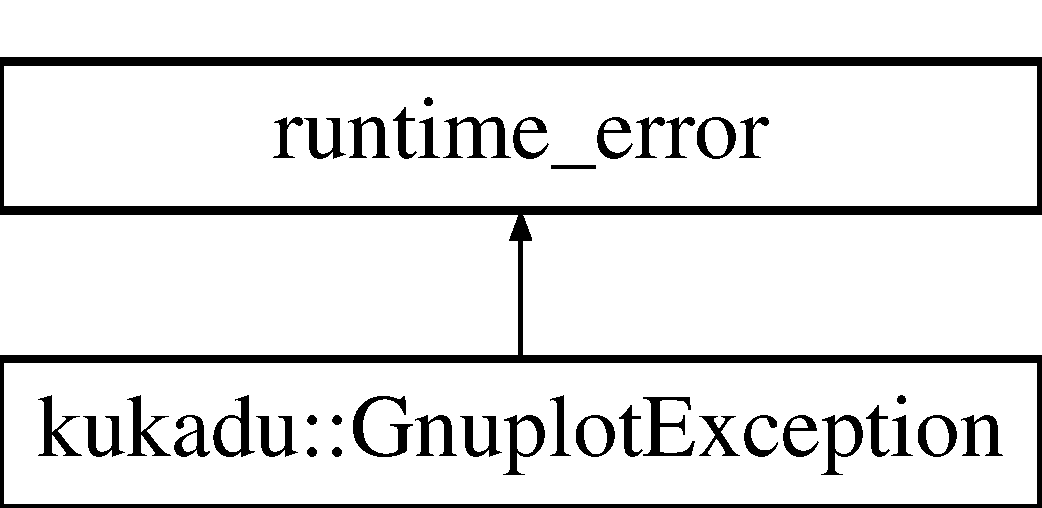
\includegraphics[height=2.000000cm]{classkukadu_1_1GnuplotException}
\end{center}
\end{figure}
\subsection*{Public Member Functions}
\begin{DoxyCompactItemize}
\item 
\hypertarget{classkukadu_1_1GnuplotException_a7bedf6ab003286b0b0cba258b6592d75}{{\bfseries Gnuplot\-Exception} (const std\-::string \&msg)}\label{classkukadu_1_1GnuplotException_a7bedf6ab003286b0b0cba258b6592d75}

\end{DoxyCompactItemize}


The documentation for this class was generated from the following file\-:\begin{DoxyCompactItemize}
\item 
/home/c7031109/iis\-\_\-robot\-\_\-sw/iis\-\_\-catkin\-\_\-ws/src/kukadu/include/kukadu/utils/gnuplot.\-hpp\end{DoxyCompactItemize}

\hypertarget{classkukadu_1_1GradientDescent}{\section{kukadu\-:\-:Gradient\-Descent Class Reference}
\label{classkukadu_1_1GradientDescent}\index{kukadu\-::\-Gradient\-Descent@{kukadu\-::\-Gradient\-Descent}}
}
Inheritance diagram for kukadu\-:\-:Gradient\-Descent\-:\begin{figure}[H]
\begin{center}
\leavevmode
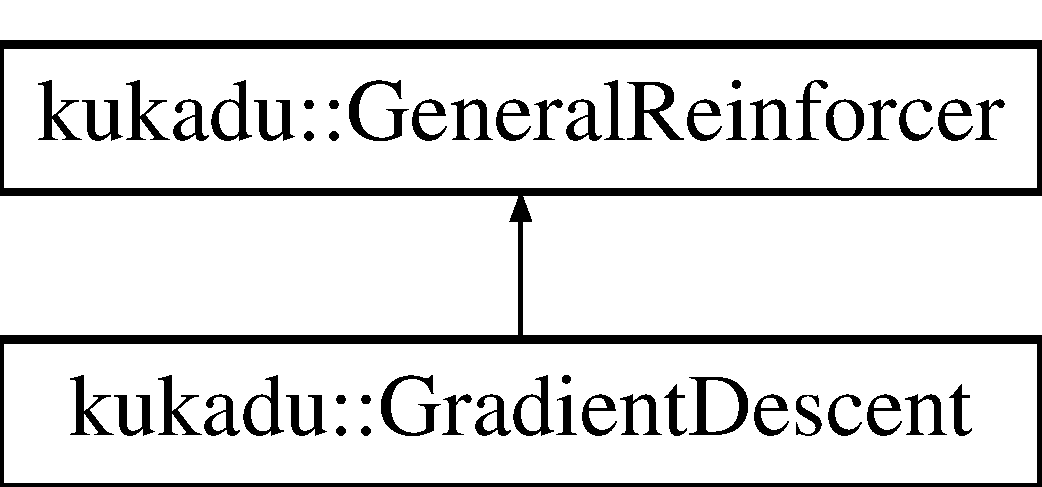
\includegraphics[height=2.000000cm]{classkukadu_1_1GradientDescent}
\end{center}
\end{figure}
\subsection*{Public Member Functions}
\begin{DoxyCompactItemize}
\item 
\hypertarget{classkukadu_1_1GradientDescent_a8d139ea3df9ad0f8d3db34a4f8d96ff0}{{\bfseries Gradient\-Descent} (K\-U\-K\-A\-D\-U\-\_\-\-S\-H\-A\-R\-E\-D\-\_\-\-P\-T\-R$<$ \hyperlink{classkukadu_1_1TrajectoryExecutor}{Trajectory\-Executor} $>$ traj\-Ex, std\-::vector$<$ K\-U\-K\-A\-D\-U\-\_\-\-S\-H\-A\-R\-E\-D\-\_\-\-P\-T\-R$<$ \hyperlink{classkukadu_1_1Trajectory}{Trajectory} $>$ $>$ init\-Dmp, double exploration\-Sigma, int updates\-Per\-Rollout, int importance\-Sampling\-Count, K\-U\-K\-A\-D\-U\-\_\-\-S\-H\-A\-R\-E\-D\-\_\-\-P\-T\-R$<$ \hyperlink{classkukadu_1_1CostComputer}{Cost\-Computer} $>$ cost, K\-U\-K\-A\-D\-U\-\_\-\-S\-H\-A\-R\-E\-D\-\_\-\-P\-T\-R$<$ \hyperlink{classkukadu_1_1ControlQueue}{Control\-Queue} $>$ simulation\-Queue, K\-U\-K\-A\-D\-U\-\_\-\-S\-H\-A\-R\-E\-D\-\_\-\-P\-T\-R$<$ \hyperlink{classkukadu_1_1ControlQueue}{Control\-Queue} $>$ execution\-Queue, double ac, double dmp\-Step\-Size, double tol\-Abs\-Err, double tol\-Rel\-Err)}\label{classkukadu_1_1GradientDescent_a8d139ea3df9ad0f8d3db34a4f8d96ff0}

\item 
\hypertarget{classkukadu_1_1GradientDescent_aff09fe5b91da1579522a19b859173d1e}{{\bfseries Gradient\-Descent} (K\-U\-K\-A\-D\-U\-\_\-\-S\-H\-A\-R\-E\-D\-\_\-\-P\-T\-R$<$ \hyperlink{classkukadu_1_1TrajectoryExecutor}{Trajectory\-Executor} $>$ traj\-Ex, std\-::vector$<$ K\-U\-K\-A\-D\-U\-\_\-\-S\-H\-A\-R\-E\-D\-\_\-\-P\-T\-R$<$ \hyperlink{classkukadu_1_1Trajectory}{Trajectory} $>$ $>$ init\-Dmp, std\-::vector$<$ double $>$ exploration\-Sigmas, int updates\-Per\-Rollout, int importance\-Sampling\-Count, K\-U\-K\-A\-D\-U\-\_\-\-S\-H\-A\-R\-E\-D\-\_\-\-P\-T\-R$<$ \hyperlink{classkukadu_1_1CostComputer}{Cost\-Computer} $>$ cost, K\-U\-K\-A\-D\-U\-\_\-\-S\-H\-A\-R\-E\-D\-\_\-\-P\-T\-R$<$ \hyperlink{classkukadu_1_1ControlQueue}{Control\-Queue} $>$ simulation\-Queue, K\-U\-K\-A\-D\-U\-\_\-\-S\-H\-A\-R\-E\-D\-\_\-\-P\-T\-R$<$ \hyperlink{classkukadu_1_1ControlQueue}{Control\-Queue} $>$ execution\-Queue, double ac, double dmp\-Step\-Size, double tol\-Abs\-Err, double tol\-Rel\-Err)}\label{classkukadu_1_1GradientDescent_aff09fe5b91da1579522a19b859173d1e}

\item 
\hypertarget{classkukadu_1_1GradientDescent_aa7238397f55b06abb5255afd327c8402}{K\-U\-K\-A\-D\-U\-\_\-\-S\-H\-A\-R\-E\-D\-\_\-\-P\-T\-R$<$ \hyperlink{classkukadu_1_1Trajectory}{Trajectory} $>$ {\bfseries update\-Step} ()}\label{classkukadu_1_1GradientDescent_aa7238397f55b06abb5255afd327c8402}

\item 
\hypertarget{classkukadu_1_1GradientDescent_a9a8a9b125c490b1eb93a1f604219fbd6}{std\-::vector$<$ K\-U\-K\-A\-D\-U\-\_\-\-S\-H\-A\-R\-E\-D\-\_\-\-P\-T\-R\\*
$<$ \hyperlink{classkukadu_1_1Trajectory}{Trajectory} $>$ $>$ \hyperlink{classkukadu_1_1GradientDescent_a9a8a9b125c490b1eb93a1f604219fbd6}{get\-Initial\-Rollout} ()}\label{classkukadu_1_1GradientDescent_a9a8a9b125c490b1eb93a1f604219fbd6}

\begin{DoxyCompactList}\small\item\em returns the first rollout of the reinforcement learning algorithm \end{DoxyCompactList}\item 
\hypertarget{classkukadu_1_1GradientDescent_abd9d198e248e55a54a346f97a5cce987}{std\-::vector$<$ K\-U\-K\-A\-D\-U\-\_\-\-S\-H\-A\-R\-E\-D\-\_\-\-P\-T\-R\\*
$<$ \hyperlink{classkukadu_1_1Trajectory}{Trajectory} $>$ $>$ \hyperlink{classkukadu_1_1GradientDescent_abd9d198e248e55a54a346f97a5cce987}{compute\-Rollout\-Paramters} ()}\label{classkukadu_1_1GradientDescent_abd9d198e248e55a54a346f97a5cce987}

\begin{DoxyCompactList}\small\item\em computes the dmp parameters for the next rollout \end{DoxyCompactList}\end{DoxyCompactItemize}


The documentation for this class was generated from the following files\-:\begin{DoxyCompactItemize}
\item 
/home/c7031109/iis\-\_\-robot\-\_\-sw/iis\-\_\-catkin\-\_\-ws/src/kukadu/include/kukadu/learning/rl/gradientdescent.\-hpp\item 
/home/c7031109/iis\-\_\-robot\-\_\-sw/iis\-\_\-catkin\-\_\-ws/src/kukadu/src/learning/reinforcement\-\_\-learning/gradientdescent.\-cpp\end{DoxyCompactItemize}

\hypertarget{structkukadu_1_1gsl__delete__expression}{\section{kukadu\-:\-:gsl\-\_\-delete\-\_\-expression Struct Reference}
\label{structkukadu_1_1gsl__delete__expression}\index{kukadu\-::gsl\-\_\-delete\-\_\-expression@{kukadu\-::gsl\-\_\-delete\-\_\-expression}}
}
\subsection*{Public Member Functions}
\begin{DoxyCompactItemize}
\item 
\hypertarget{structkukadu_1_1gsl__delete__expression_a2eef07907659d92f2165f0584fa59c81}{void {\bfseries operator()} (gsl\-\_\-odeiv2\-\_\-driver $\ast$p) const }\label{structkukadu_1_1gsl__delete__expression_a2eef07907659d92f2165f0584fa59c81}

\end{DoxyCompactItemize}


The documentation for this struct was generated from the following file\-:\begin{DoxyCompactItemize}
\item 
/home/c7031109/iis\-\_\-robot\-\_\-sw/iis\-\_\-catkin\-\_\-ws/src/kukadu/include/kukadu/control/dmpexecutor.\-hpp\end{DoxyCompactItemize}

\hypertarget{classkukadu_1_1HapticControllerResult}{\section{kukadu\-:\-:Haptic\-Controller\-Result Class Reference}
\label{classkukadu_1_1HapticControllerResult}\index{kukadu\-::\-Haptic\-Controller\-Result@{kukadu\-::\-Haptic\-Controller\-Result}}
}
Inheritance diagram for kukadu\-:\-:Haptic\-Controller\-Result\-:\begin{figure}[H]
\begin{center}
\leavevmode
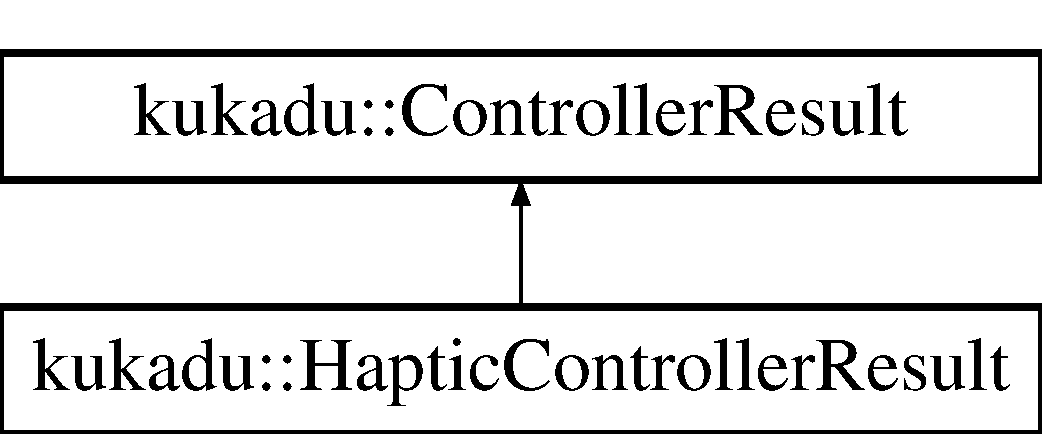
\includegraphics[height=2.000000cm]{classkukadu_1_1HapticControllerResult}
\end{center}
\end{figure}
\subsection*{Public Member Functions}
\begin{DoxyCompactItemize}
\item 
\hypertarget{classkukadu_1_1HapticControllerResult_a47345ffc29dd31ecb607327272e22f77}{{\bfseries Haptic\-Controller\-Result} (arma\-::vec t, std\-::vector$<$ arma\-::vec $>$ ys, bool success, bool bored, std\-::vector$<$ int $>$ walked\-Path, K\-U\-K\-A\-D\-U\-\_\-\-S\-H\-A\-R\-E\-D\-\_\-\-P\-T\-R$<$ std\-::tuple$<$ double, K\-U\-K\-A\-D\-U\-\_\-\-S\-H\-A\-R\-E\-D\-\_\-\-P\-T\-R$<$ \hyperlink{classkukadu_1_1Clip}{kukadu\-::\-Clip} $>$, std\-::vector$<$ K\-U\-K\-A\-D\-U\-\_\-\-S\-H\-A\-R\-E\-D\-\_\-\-P\-T\-R$<$ \hyperlink{classkukadu_1_1Clip}{kukadu\-::\-Clip} $>$ $>$ $>$ $>$ environment\-Transition)}\label{classkukadu_1_1HapticControllerResult_a47345ffc29dd31ecb607327272e22f77}

\item 
\hypertarget{classkukadu_1_1HapticControllerResult_a9de0d818f4846a50824982a206093174}{bool {\bfseries was\-Bored} ()}\label{classkukadu_1_1HapticControllerResult_a9de0d818f4846a50824982a206093174}

\item 
\hypertarget{classkukadu_1_1HapticControllerResult_ad22c014f12ae0bff2c24edc4cce7fd32}{std\-::vector$<$ int $>$ {\bfseries get\-Walked\-Path} ()}\label{classkukadu_1_1HapticControllerResult_ad22c014f12ae0bff2c24edc4cce7fd32}

\end{DoxyCompactItemize}


The documentation for this class was generated from the following files\-:\begin{DoxyCompactItemize}
\item 
/home/c7031109/iis\-\_\-robot\-\_\-sw/iis\-\_\-catkin\-\_\-ws/src/kukadu/include/kukadu/types/controllerresult.\-hpp\item 
/home/c7031109/iis\-\_\-robot\-\_\-sw/iis\-\_\-catkin\-\_\-ws/src/kukadu/src/types/controllerresult.\-cpp\end{DoxyCompactItemize}

\hypertarget{classkukadu_1_1HapticPlanner}{\section{kukadu\-:\-:Haptic\-Planner Class Reference}
\label{classkukadu_1_1HapticPlanner}\index{kukadu\-::\-Haptic\-Planner@{kukadu\-::\-Haptic\-Planner}}
}
Inheritance diagram for kukadu\-:\-:Haptic\-Planner\-:\begin{figure}[H]
\begin{center}
\leavevmode
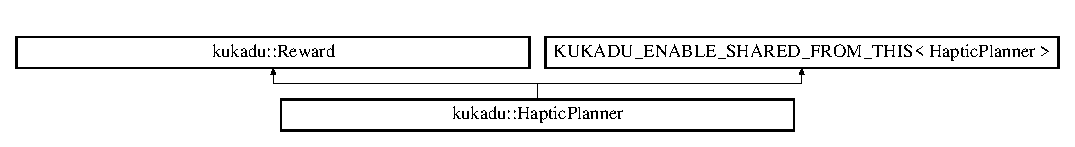
\includegraphics[height=1.530055cm]{classkukadu_1_1HapticPlanner}
\end{center}
\end{figure}
\subsection*{Public Member Functions}
\begin{DoxyCompactItemize}
\item 
\hypertarget{classkukadu_1_1HapticPlanner_a7b2694b3c164abd63094612a7f8b020a}{{\bfseries Haptic\-Planner} (std\-::string skill\-Database, std\-::vector$<$ K\-U\-K\-A\-D\-U\-\_\-\-S\-H\-A\-R\-E\-D\-\_\-\-P\-T\-R$<$ \hyperlink{classkukadu_1_1SensingController}{kukadu\-::\-Sensing\-Controller} $>$ $>$ sensing\-Controllers, std\-::vector$<$ K\-U\-K\-A\-D\-U\-\_\-\-S\-H\-A\-R\-E\-D\-\_\-\-P\-T\-R$<$ \hyperlink{classkukadu_1_1Controller}{kukadu\-::\-Controller} $>$ $>$ preparatory\-Controllers, std\-::vector$<$ K\-U\-K\-A\-D\-U\-\_\-\-S\-H\-A\-R\-E\-D\-\_\-\-P\-T\-R$<$ \hyperlink{classkukadu_1_1Controller}{kukadu\-::\-Controller} $>$ $>$ complex\-Controllers, K\-U\-K\-A\-D\-U\-\_\-\-S\-H\-A\-R\-E\-D\-\_\-\-P\-T\-R$<$ \hyperlink{classkukadu_1_1Controller}{kukadu\-::\-Controller} $>$ nothing\-Controller, K\-U\-K\-A\-D\-U\-\_\-\-S\-H\-A\-R\-E\-D\-\_\-\-P\-T\-R$<$ kukadu\-\_\-mersenne\-\_\-twister $>$ generator)}\label{classkukadu_1_1HapticPlanner_a7b2694b3c164abd63094612a7f8b020a}

\item 
\hypertarget{classkukadu_1_1HapticPlanner_a8e5fe565402949ff974a32bd1a895883}{virtual int {\bfseries get\-Dimensionality} ()}\label{classkukadu_1_1HapticPlanner_a8e5fe565402949ff974a32bd1a895883}

\item 
\hypertarget{classkukadu_1_1HapticPlanner_a588f0364647cff1401ce4eae9d819f47}{virtual K\-U\-K\-A\-D\-U\-\_\-\-S\-H\-A\-R\-E\-D\-\_\-\-P\-T\-R\\*
$<$ \hyperlink{classkukadu_1_1PerceptClip}{Percept\-Clip} $>$ {\bfseries generate\-Next\-Percept\-Clip} (int immunity)}\label{classkukadu_1_1HapticPlanner_a588f0364647cff1401ce4eae9d819f47}

\item 
\hypertarget{classkukadu_1_1HapticPlanner_aa386d3e94482e5181626c1eddebffd7b}{virtual K\-U\-K\-A\-D\-U\-\_\-\-S\-H\-A\-R\-E\-D\-\_\-\-P\-T\-R\\*
$<$ std\-::vector\\*
$<$ K\-U\-K\-A\-D\-U\-\_\-\-S\-H\-A\-R\-E\-D\-\_\-\-P\-T\-R\\*
$<$ \hyperlink{classkukadu_1_1ActionClip}{Action\-Clip} $>$ $>$ $>$ {\bfseries generate\-Action\-Clips} ()}\label{classkukadu_1_1HapticPlanner_aa386d3e94482e5181626c1eddebffd7b}

\item 
\hypertarget{classkukadu_1_1HapticPlanner_a9748d448f421504336013c4aa98e243d}{virtual K\-U\-K\-A\-D\-U\-\_\-\-S\-H\-A\-R\-E\-D\-\_\-\-P\-T\-R\\*
$<$ std\-::vector\\*
$<$ K\-U\-K\-A\-D\-U\-\_\-\-S\-H\-A\-R\-E\-D\-\_\-\-P\-T\-R\\*
$<$ \hyperlink{classkukadu_1_1PerceptClip}{Percept\-Clip} $>$ $>$ $>$ {\bfseries generate\-Percept\-Clips} ()}\label{classkukadu_1_1HapticPlanner_a9748d448f421504336013c4aa98e243d}

\item 
\hypertarget{classkukadu_1_1HapticPlanner_a267e6afa41919c58b1a37bd0e460dfb9}{void {\bfseries pick\-And\-Perform\-Complex\-Skill} (bool update\-Models=true)}\label{classkukadu_1_1HapticPlanner_a267e6afa41919c58b1a37bd0e460dfb9}

\item 
\hypertarget{classkukadu_1_1HapticPlanner_ac8eb5e6c2b41dc7766c1503b50541302}{K\-U\-K\-A\-D\-U\-\_\-\-S\-H\-A\-R\-E\-D\-\_\-\-P\-T\-R\\*
$<$ \hyperlink{classkukadu_1_1HapticControllerResult}{kukadu\-::\-Haptic\-Controller\-Result} $>$ {\bfseries perform\-Complex\-Skill} (std\-::string skill\-Id, bool update\-Models=true)}\label{classkukadu_1_1HapticPlanner_ac8eb5e6c2b41dc7766c1503b50541302}

\item 
\hypertarget{classkukadu_1_1HapticPlanner_a2ed1772fee9f9b2dc4930b66896cb5ff}{void {\bfseries update\-Models} ()}\label{classkukadu_1_1HapticPlanner_a2ed1772fee9f9b2dc4930b66896cb5ff}

\item 
\hypertarget{classkukadu_1_1HapticPlanner_a87764109bd04a93c93f91a37de9dd214}{std\-::string {\bfseries pick\-Complex\-Skill} ()}\label{classkukadu_1_1HapticPlanner_a87764109bd04a93c93f91a37de9dd214}

\item 
\hypertarget{classkukadu_1_1HapticPlanner_afc97d78845cd9675993f352845c5c02e}{void {\bfseries set\-Simulation\-Mode} (bool simulation\-Mode)}\label{classkukadu_1_1HapticPlanner_afc97d78845cd9675993f352845c5c02e}

\end{DoxyCompactItemize}
\subsection*{Protected Member Functions}
\begin{DoxyCompactItemize}
\item 
\hypertarget{classkukadu_1_1HapticPlanner_a8d73a2aa0ca782970a1885a7b8970e5f}{virtual double {\bfseries compute\-Reward\-Internal} (K\-U\-K\-A\-D\-U\-\_\-\-S\-H\-A\-R\-E\-D\-\_\-\-P\-T\-R$<$ \hyperlink{classkukadu_1_1PerceptClip}{Percept\-Clip} $>$ provided\-Percept, K\-U\-K\-A\-D\-U\-\_\-\-S\-H\-A\-R\-E\-D\-\_\-\-P\-T\-R$<$ \hyperlink{classkukadu_1_1ActionClip}{Action\-Clip} $>$ taken\-Action)}\label{classkukadu_1_1HapticPlanner_a8d73a2aa0ca782970a1885a7b8970e5f}

\end{DoxyCompactItemize}
\subsection*{Additional Inherited Members}


The documentation for this class was generated from the following files\-:\begin{DoxyCompactItemize}
\item 
/home/c7031109/iis\-\_\-robot\-\_\-sw/iis\-\_\-catkin\-\_\-ws/src/kukadu/include/kukadu/manipulation/haptic/hapticplanner.\-hpp\item 
/home/c7031109/iis\-\_\-robot\-\_\-sw/iis\-\_\-catkin\-\_\-ws/src/kukadu/src/manipulation/haptic/hapticplanner.\-cpp\end{DoxyCompactItemize}

\hypertarget{classkukadu_1_1InfTheoConstraints}{\section{kukadu\-:\-:Inf\-Theo\-Constraints Class Reference}
\label{classkukadu_1_1InfTheoConstraints}\index{kukadu\-::\-Inf\-Theo\-Constraints@{kukadu\-::\-Inf\-Theo\-Constraints}}
}
\subsection*{Public Member Functions}
\begin{DoxyCompactItemize}
\item 
\hypertarget{classkukadu_1_1InfTheoConstraints_aa25c31a3ac239b93ca899d5c0dab9f49}{void {\bfseries add\-Constraint} (arma\-::vec x1, arma\-::vec x2, double slack)}\label{classkukadu_1_1InfTheoConstraints_aa25c31a3ac239b93ca899d5c0dab9f49}

\item 
\hypertarget{classkukadu_1_1InfTheoConstraints_ac1d85733f326e20e6900ad3debafda0f}{void {\bfseries flush} ()}\label{classkukadu_1_1InfTheoConstraints_ac1d85733f326e20e6900ad3debafda0f}

\item 
\hypertarget{classkukadu_1_1InfTheoConstraints_a722ffde92b39ab76c9fde6629acbebf6}{int {\bfseries get\-Constraint\-Count} ()}\label{classkukadu_1_1InfTheoConstraints_a722ffde92b39ab76c9fde6629acbebf6}

\item 
\hypertarget{classkukadu_1_1InfTheoConstraints_a085b65427f852bad0414f758cd21821e}{arma\-::vec {\bfseries get\-X1} (int idx)}\label{classkukadu_1_1InfTheoConstraints_a085b65427f852bad0414f758cd21821e}

\item 
\hypertarget{classkukadu_1_1InfTheoConstraints_aea03b865c1285775b57fcf88f1d7104c}{arma\-::vec {\bfseries get\-X2} (int idx)}\label{classkukadu_1_1InfTheoConstraints_aea03b865c1285775b57fcf88f1d7104c}

\item 
\hypertarget{classkukadu_1_1InfTheoConstraints_ac006e5b1d58e8fbea8985786766d6596}{double {\bfseries get\-Slack} (int idx)}\label{classkukadu_1_1InfTheoConstraints_ac006e5b1d58e8fbea8985786766d6596}

\item 
\hypertarget{classkukadu_1_1InfTheoConstraints_a164b756056c091f61414275c05617b01}{double {\bfseries get\-Lambda} (int idx)}\label{classkukadu_1_1InfTheoConstraints_a164b756056c091f61414275c05617b01}

\item 
\hypertarget{classkukadu_1_1InfTheoConstraints_adb17a3786b877a8001051697131349c4}{void {\bfseries set\-Slack} (int idx, double slack)}\label{classkukadu_1_1InfTheoConstraints_adb17a3786b877a8001051697131349c4}

\item 
\hypertarget{classkukadu_1_1InfTheoConstraints_ac418da12a5d931c5acee6dc724123f3a}{void {\bfseries set\-Lambda} (int idx, double lambda)}\label{classkukadu_1_1InfTheoConstraints_ac418da12a5d931c5acee6dc724123f3a}

\end{DoxyCompactItemize}


The documentation for this class was generated from the following files\-:\begin{DoxyCompactItemize}
\item 
/home/c7031109/iis\-\_\-robot\-\_\-sw/iis\-\_\-catkin\-\_\-ws/src/kukadu/include/kukadu/learning/metric\-\_\-learning/inftheoconstraints.\-hpp\item 
/home/c7031109/iis\-\_\-robot\-\_\-sw/iis\-\_\-catkin\-\_\-ws/src/kukadu/src/learning/metric\-\_\-learning/inftheoconstraints.\-cpp\end{DoxyCompactItemize}

\hypertarget{classkukadu_1_1InfTheoMetricLearner}{\section{kukadu\-:\-:Inf\-Theo\-Metric\-Learner Class Reference}
\label{classkukadu_1_1InfTheoMetricLearner}\index{kukadu\-::\-Inf\-Theo\-Metric\-Learner@{kukadu\-::\-Inf\-Theo\-Metric\-Learner}}
}
Inheritance diagram for kukadu\-:\-:Inf\-Theo\-Metric\-Learner\-:\begin{figure}[H]
\begin{center}
\leavevmode
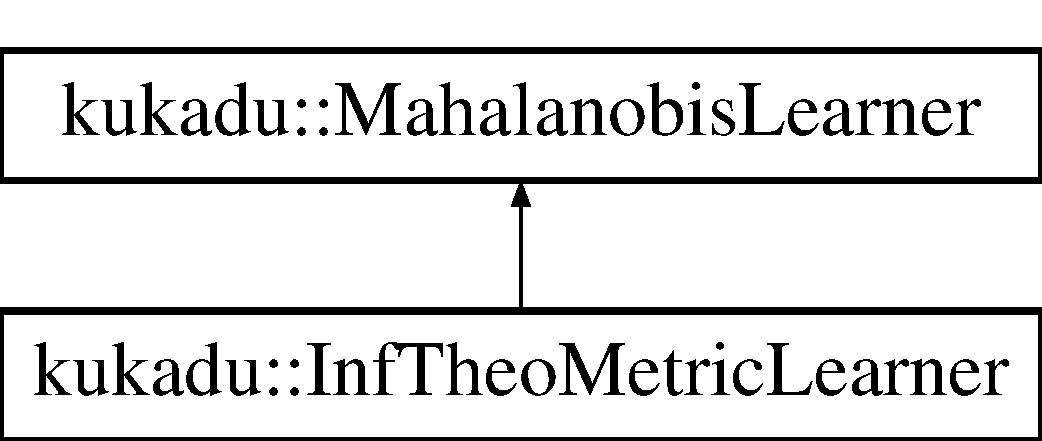
\includegraphics[height=2.000000cm]{classkukadu_1_1InfTheoMetricLearner}
\end{center}
\end{figure}
\subsection*{Public Member Functions}
\begin{DoxyCompactItemize}
\item 
\hypertarget{classkukadu_1_1InfTheoMetricLearner_a7d69af547c7d4337a7469662628a35b6}{{\bfseries Inf\-Theo\-Metric\-Learner} (std\-::vector$<$ arma\-::vec $>$ x1s, std\-::vector$<$ arma\-::vec $>$ x2s, std\-::vector$<$ double $>$ distances, double sim\-Border, double dis\-Sim\-Border, double gamma, double div\-Tol, int check\-For\-Con\-Count)}\label{classkukadu_1_1InfTheoMetricLearner_a7d69af547c7d4337a7469662628a35b6}

\item 
\hypertarget{classkukadu_1_1InfTheoMetricLearner_ada74ff5d257bf64a5c3e1a4ba910148d}{\hyperlink{classkukadu_1_1Mahalanobis}{Mahalanobis} {\bfseries learn\-Metric} ()}\label{classkukadu_1_1InfTheoMetricLearner_ada74ff5d257bf64a5c3e1a4ba910148d}

\end{DoxyCompactItemize}
\subsection*{Additional Inherited Members}


The documentation for this class was generated from the following files\-:\begin{DoxyCompactItemize}
\item 
/home/c7031109/iis\-\_\-robot\-\_\-sw/iis\-\_\-catkin\-\_\-ws/src/kukadu/include/kukadu/learning/metric\-\_\-learning/inftheometriclearner.\-hpp\item 
/home/c7031109/iis\-\_\-robot\-\_\-sw/iis\-\_\-catkin\-\_\-ws/src/kukadu/src/learning/metric\-\_\-learning/inftheometriclearner.\-cpp\end{DoxyCompactItemize}

\hypertarget{classkukadu_1_1IntermediateEventClip}{\section{kukadu\-:\-:Intermediate\-Event\-Clip Class Reference}
\label{classkukadu_1_1IntermediateEventClip}\index{kukadu\-::\-Intermediate\-Event\-Clip@{kukadu\-::\-Intermediate\-Event\-Clip}}
}
Inheritance diagram for kukadu\-:\-:Intermediate\-Event\-Clip\-:\begin{figure}[H]
\begin{center}
\leavevmode
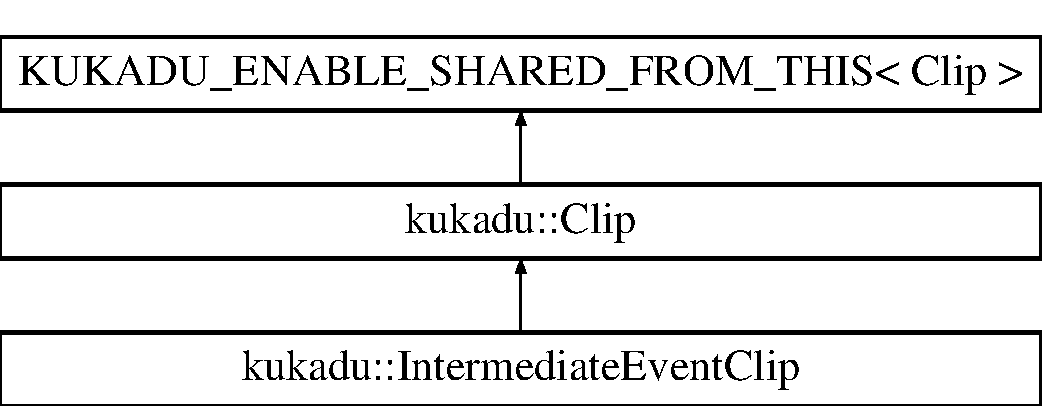
\includegraphics[height=3.000000cm]{classkukadu_1_1IntermediateEventClip}
\end{center}
\end{figure}
\subsection*{Public Member Functions}
\begin{DoxyCompactItemize}
\item 
\hypertarget{classkukadu_1_1IntermediateEventClip_a91279d5477030bfdd9adf95864fbff04}{{\bfseries Intermediate\-Event\-Clip} (K\-U\-K\-A\-D\-U\-\_\-\-S\-H\-A\-R\-E\-D\-\_\-\-P\-T\-R$<$ \hyperlink{classkukadu_1_1SensingController}{Sensing\-Controller} $>$ sensing\-Event, int level, K\-U\-K\-A\-D\-U\-\_\-\-S\-H\-A\-R\-E\-D\-\_\-\-P\-T\-R$<$ kukadu\-\_\-mersenne\-\_\-twister $>$ generator, std\-::string clip\-Values, int immunity)}\label{classkukadu_1_1IntermediateEventClip_a91279d5477030bfdd9adf95864fbff04}

\item 
\hypertarget{classkukadu_1_1IntermediateEventClip_a880dddcacad2b7cd26be43bdf62cd11a}{{\bfseries Intermediate\-Event\-Clip} (K\-U\-K\-A\-D\-U\-\_\-\-S\-H\-A\-R\-E\-D\-\_\-\-P\-T\-R$<$ \hyperlink{classkukadu_1_1SensingController}{Sensing\-Controller} $>$ sensing\-Event, int level, K\-U\-K\-A\-D\-U\-\_\-\-S\-H\-A\-R\-E\-D\-\_\-\-P\-T\-R$<$ kukadu\-\_\-mersenne\-\_\-twister $>$ generator, K\-U\-K\-A\-D\-U\-\_\-\-S\-H\-A\-R\-E\-D\-\_\-\-P\-T\-R$<$ std\-::vector$<$ int $>$ $>$ clip\-Values, int immunity)}\label{classkukadu_1_1IntermediateEventClip_a880dddcacad2b7cd26be43bdf62cd11a}

\item 
\hypertarget{classkukadu_1_1IntermediateEventClip_aa2aeb835bcd24ad8503ddebee554fbac}{virtual std\-::string {\bfseries to\-String} () const }\label{classkukadu_1_1IntermediateEventClip_aa2aeb835bcd24ad8503ddebee554fbac}

\item 
\hypertarget{classkukadu_1_1IntermediateEventClip_a471a55d04d08972093c618d383af1213}{std\-::pair$<$ int, \\*
K\-U\-K\-A\-D\-U\-\_\-\-S\-H\-A\-R\-E\-D\-\_\-\-P\-T\-R$<$ \hyperlink{classkukadu_1_1Clip}{Clip} $>$ $>$ {\bfseries jump\-Next\-Random} ()}\label{classkukadu_1_1IntermediateEventClip_a471a55d04d08972093c618d383af1213}

\item 
\hypertarget{classkukadu_1_1IntermediateEventClip_af486d261e5b163d86b5bfe87fd7a41a7}{K\-U\-K\-A\-D\-U\-\_\-\-S\-H\-A\-R\-E\-D\-\_\-\-P\-T\-R\\*
$<$ \hyperlink{classkukadu_1_1SensingController}{Sensing\-Controller} $>$ {\bfseries get\-Sensing\-Controller} ()}\label{classkukadu_1_1IntermediateEventClip_af486d261e5b163d86b5bfe87fd7a41a7}

\end{DoxyCompactItemize}
\subsection*{Additional Inherited Members}


The documentation for this class was generated from the following files\-:\begin{DoxyCompactItemize}
\item 
/home/c7031109/iis\-\_\-robot\-\_\-sw/iis\-\_\-catkin\-\_\-ws/src/kukadu/include/kukadu/manipulation/haptic/intermediateeventclip.\-hpp\item 
/home/c7031109/iis\-\_\-robot\-\_\-sw/iis\-\_\-catkin\-\_\-ws/src/kukadu/src/manipulation/haptic/intermediateeventclip.\-cpp\end{DoxyCompactItemize}

\hypertarget{classkukadu_1_1InvasionGameReward}{\section{kukadu\-:\-:Invasion\-Game\-Reward Class Reference}
\label{classkukadu_1_1InvasionGameReward}\index{kukadu\-::\-Invasion\-Game\-Reward@{kukadu\-::\-Invasion\-Game\-Reward}}
}
Inheritance diagram for kukadu\-:\-:Invasion\-Game\-Reward\-:\begin{figure}[H]
\begin{center}
\leavevmode
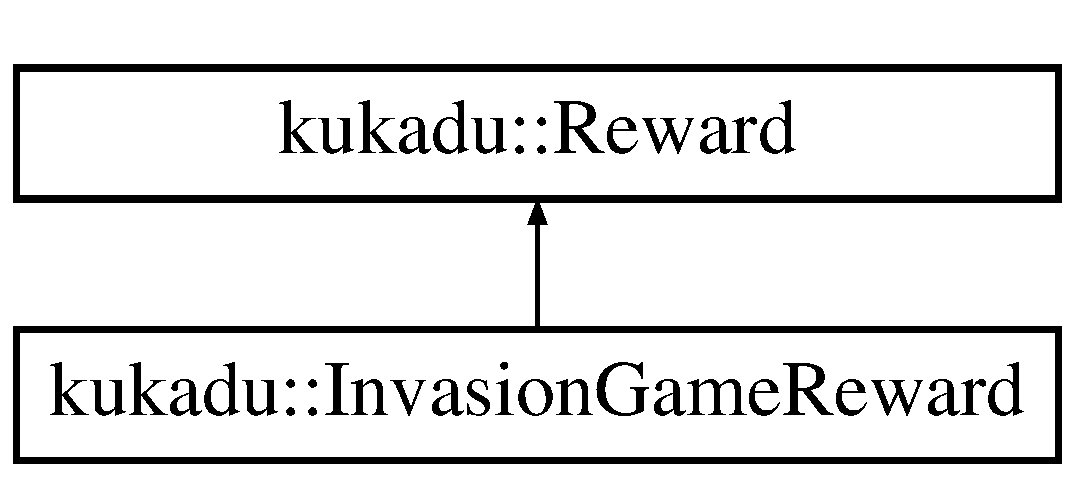
\includegraphics[height=2.000000cm]{classkukadu_1_1InvasionGameReward}
\end{center}
\end{figure}
\subsection*{Public Member Functions}
\begin{DoxyCompactItemize}
\item 
\hypertarget{classkukadu_1_1InvasionGameReward_aa155bb350d87b7f006165b71bf703ca7}{{\bfseries Invasion\-Game\-Reward} (K\-U\-K\-A\-D\-U\-\_\-\-S\-H\-A\-R\-E\-D\-\_\-\-P\-T\-R$<$ kukadu\-\_\-mersenne\-\_\-twister $>$ generator, bool collect\-Prev\-Rewards)}\label{classkukadu_1_1InvasionGameReward_aa155bb350d87b7f006165b71bf703ca7}

\item 
\hypertarget{classkukadu_1_1InvasionGameReward_a3cdd9b9d8e3d60295e8a6db8227ffcda}{int {\bfseries get\-Dimensionality} ()}\label{classkukadu_1_1InvasionGameReward_a3cdd9b9d8e3d60295e8a6db8227ffcda}

\item 
\hypertarget{classkukadu_1_1InvasionGameReward_ab83c35cfccb53e8547a92dac69f13005}{K\-U\-K\-A\-D\-U\-\_\-\-S\-H\-A\-R\-E\-D\-\_\-\-P\-T\-R$<$ \hyperlink{classkukadu_1_1PerceptClip}{Percept\-Clip} $>$ {\bfseries generate\-Next\-Percept\-Clip} (int immunity)}\label{classkukadu_1_1InvasionGameReward_ab83c35cfccb53e8547a92dac69f13005}

\item 
\hypertarget{classkukadu_1_1InvasionGameReward_a729d7ae52ab945b1520a9d24ee2ffba7}{K\-U\-K\-A\-D\-U\-\_\-\-S\-H\-A\-R\-E\-D\-\_\-\-P\-T\-R$<$ std\-::vector\\*
$<$ K\-U\-K\-A\-D\-U\-\_\-\-S\-H\-A\-R\-E\-D\-\_\-\-P\-T\-R\\*
$<$ \hyperlink{classkukadu_1_1ActionClip}{Action\-Clip} $>$ $>$ $>$ {\bfseries generate\-Action\-Clips} ()}\label{classkukadu_1_1InvasionGameReward_a729d7ae52ab945b1520a9d24ee2ffba7}

\item 
\hypertarget{classkukadu_1_1InvasionGameReward_a2945179e42d2cffd8c8f8bce264dcc0d}{K\-U\-K\-A\-D\-U\-\_\-\-S\-H\-A\-R\-E\-D\-\_\-\-P\-T\-R$<$ std\-::vector\\*
$<$ K\-U\-K\-A\-D\-U\-\_\-\-S\-H\-A\-R\-E\-D\-\_\-\-P\-T\-R\\*
$<$ \hyperlink{classkukadu_1_1PerceptClip}{Percept\-Clip} $>$ $>$ $>$ {\bfseries generate\-Percept\-Clips} ()}\label{classkukadu_1_1InvasionGameReward_a2945179e42d2cffd8c8f8bce264dcc0d}

\end{DoxyCompactItemize}
\subsection*{Protected Member Functions}
\begin{DoxyCompactItemize}
\item 
\hypertarget{classkukadu_1_1InvasionGameReward_abe8b92de8b073852651facf9e2b2b29d}{double {\bfseries compute\-Reward\-Internal} (K\-U\-K\-A\-D\-U\-\_\-\-S\-H\-A\-R\-E\-D\-\_\-\-P\-T\-R$<$ \hyperlink{classkukadu_1_1PerceptClip}{Percept\-Clip} $>$ provided\-Percept, K\-U\-K\-A\-D\-U\-\_\-\-S\-H\-A\-R\-E\-D\-\_\-\-P\-T\-R$<$ \hyperlink{classkukadu_1_1ActionClip}{Action\-Clip} $>$ taken\-Action)}\label{classkukadu_1_1InvasionGameReward_abe8b92de8b073852651facf9e2b2b29d}

\end{DoxyCompactItemize}
\subsection*{Additional Inherited Members}


The documentation for this class was generated from the following files\-:\begin{DoxyCompactItemize}
\item 
/home/c7031109/iis\-\_\-robot\-\_\-sw/iis\-\_\-catkin\-\_\-ws/src/kukadu/include/kukadu/learning/projective\-\_\-simulation/application/invasiongamereward.\-hpp\item 
/home/c7031109/iis\-\_\-robot\-\_\-sw/iis\-\_\-catkin\-\_\-ws/src/kukadu/src/learning/projective\-\_\-simulation/application/invasiongamereward.\-cpp\end{DoxyCompactItemize}

\hypertarget{classkukadu_1_1JointDmp}{\section{kukadu\-:\-:Joint\-Dmp Class Reference}
\label{classkukadu_1_1JointDmp}\index{kukadu\-::\-Joint\-Dmp@{kukadu\-::\-Joint\-Dmp}}
}
Inheritance diagram for kukadu\-:\-:Joint\-Dmp\-:\begin{figure}[H]
\begin{center}
\leavevmode
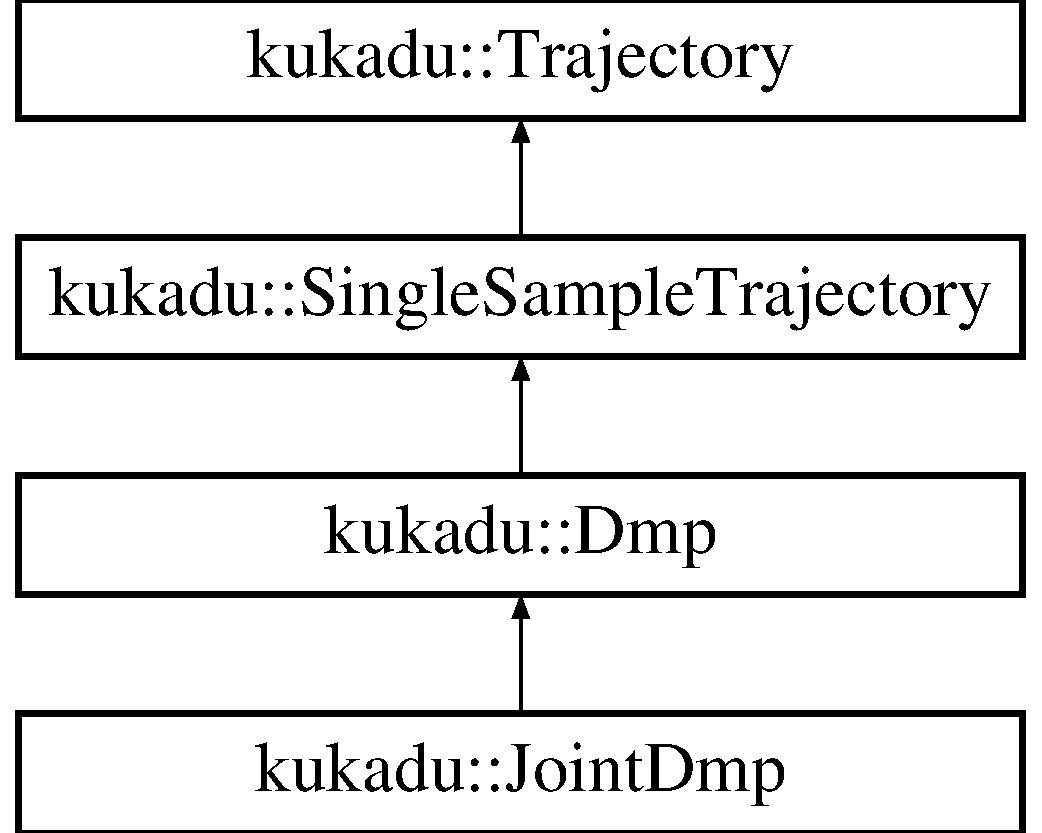
\includegraphics[height=4.000000cm]{classkukadu_1_1JointDmp}
\end{center}
\end{figure}
\subsection*{Public Member Functions}
\begin{DoxyCompactItemize}
\item 
\hypertarget{classkukadu_1_1JointDmp_a2f2b43e39e2d7ece9ad0a958ccbac8e8}{{\bfseries Joint\-Dmp} (arma\-::vec supervised\-Ts, std\-::vector$<$ arma\-::vec $>$ sample\-Ys, std\-::vector$<$ arma\-::vec $>$ fit\-Ys, std\-::vector$<$ arma\-::vec $>$ dmp\-Coeffs, std\-::vector$<$ \hyperlink{classkukadu_1_1DMPBase}{D\-M\-P\-Base} $>$ dmp\-Base, std\-::vector$<$ arma\-::mat $>$ design\-Matrices, double tau, double az, double bz, double ax, double ac, double dmp\-Step\-Size, double tol\-Abs\-Err, double tol\-Rel\-Err)}\label{classkukadu_1_1JointDmp_a2f2b43e39e2d7ece9ad0a958ccbac8e8}

\item 
\hypertarget{classkukadu_1_1JointDmp_a58dc179759c2a9ebbbfe6d13cf65794c}{{\bfseries Joint\-Dmp} (arma\-::vec supervised\-Ts, std\-::vector$<$ arma\-::vec $>$ sample\-Ys, std\-::vector$<$ arma\-::vec $>$ fit\-Ys, std\-::vector$<$ arma\-::vec $>$ dmp\-Coeffs, std\-::vector$<$ \hyperlink{classkukadu_1_1DMPBase}{D\-M\-P\-Base} $>$ dmp\-Base, std\-::vector$<$ arma\-::mat $>$ design\-Matrices, double tau, double az, double bz, double ax)}\label{classkukadu_1_1JointDmp_a58dc179759c2a9ebbbfe6d13cf65794c}

\item 
\hypertarget{classkukadu_1_1JointDmp_a4984be2815b7a0b1e6f14ecee33593b2}{{\bfseries Joint\-Dmp} (std\-::string dmp\-File)}\label{classkukadu_1_1JointDmp_a4984be2815b7a0b1e6f14ecee33593b2}

\item 
\hypertarget{classkukadu_1_1JointDmp_a12d8909497b9d4f38c1cac86a1ad6601}{bool {\bfseries is\-Cartesian} ()}\label{classkukadu_1_1JointDmp_a12d8909497b9d4f38c1cac86a1ad6601}

\item 
\hypertarget{classkukadu_1_1JointDmp_ac3fd610d7a8e2f74143071d06ae04290}{virtual K\-U\-K\-A\-D\-U\-\_\-\-S\-H\-A\-R\-E\-D\-\_\-\-P\-T\-R\\*
$<$ \hyperlink{classkukadu_1_1Trajectory}{Trajectory} $>$ {\bfseries copy} ()}\label{classkukadu_1_1JointDmp_ac3fd610d7a8e2f74143071d06ae04290}

\end{DoxyCompactItemize}
\subsection*{Additional Inherited Members}


The documentation for this class was generated from the following files\-:\begin{DoxyCompactItemize}
\item 
/home/c7031109/iis\-\_\-robot\-\_\-sw/iis\-\_\-catkin\-\_\-ws/src/kukadu/include/kukadu/types/jointdmp.\-hpp\item 
/home/c7031109/iis\-\_\-robot\-\_\-sw/iis\-\_\-catkin\-\_\-ws/src/kukadu/src/types/jointdmp.\-cpp\end{DoxyCompactItemize}

\hypertarget{classkukadu_1_1JointDMPLearner}{\section{kukadu\-:\-:Joint\-D\-M\-P\-Learner Class Reference}
\label{classkukadu_1_1JointDMPLearner}\index{kukadu\-::\-Joint\-D\-M\-P\-Learner@{kukadu\-::\-Joint\-D\-M\-P\-Learner}}
}


The Trajectory\-D\-M\-P\-Learner encapsulates the dmp learning process.  




{\ttfamily \#include $<$jointdmplearner.\-hpp$>$}

Inheritance diagram for kukadu\-:\-:Joint\-D\-M\-P\-Learner\-:\begin{figure}[H]
\begin{center}
\leavevmode
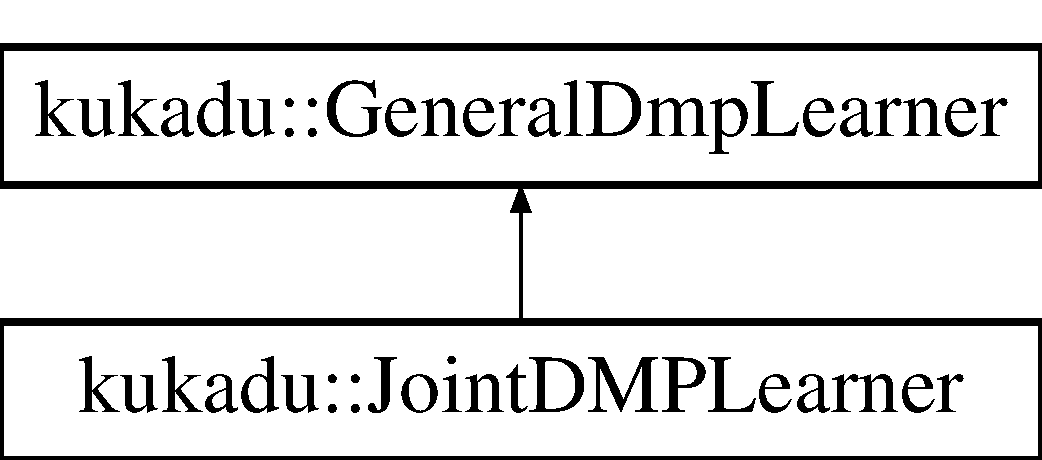
\includegraphics[height=2.000000cm]{classkukadu_1_1JointDMPLearner}
\end{center}
\end{figure}
\subsection*{Public Member Functions}
\begin{DoxyCompactItemize}
\item 
\hyperlink{classkukadu_1_1JointDMPLearner_aeafe6581d82892f4038e0087f80c48c9}{Joint\-D\-M\-P\-Learner} (std\-::vector$<$ \hyperlink{classkukadu_1_1DMPBase}{D\-M\-P\-Base} $>$ dmp\-Base, double tau, double az, double bz, double ax, arma\-::mat joints)
\begin{DoxyCompactList}\small\item\em constructor \end{DoxyCompactList}\item 
\hyperlink{classkukadu_1_1JointDMPLearner_a0831ec240ee08b99bef99d4e2806f31f}{Joint\-D\-M\-P\-Learner} (std\-::vector$<$ double $>$ mys\-Def, std\-::vector$<$ double $>$ sigmas\-Def, double az, double bz, std\-::string file)
\begin{DoxyCompactList}\small\item\em constructor \end{DoxyCompactList}\item 
\hypertarget{classkukadu_1_1JointDMPLearner_a40e29048662ca3a660993654e36db047}{{\bfseries Joint\-D\-M\-P\-Learner} (double az, double bz, std\-::string file)}\label{classkukadu_1_1JointDMPLearner_a40e29048662ca3a660993654e36db047}

\item 
\hypertarget{classkukadu_1_1JointDMPLearner_a96029d28387b06bba16bc2ccd3965cae}{{\bfseries Joint\-D\-M\-P\-Learner} (double az, double bz, arma\-::mat joints)}\label{classkukadu_1_1JointDMPLearner_a96029d28387b06bba16bc2ccd3965cae}

\end{DoxyCompactItemize}
\subsection*{Protected Member Functions}
\begin{DoxyCompactItemize}
\item 
\hypertarget{classkukadu_1_1JointDMPLearner_ac16e6c7d24bbdf194663bdc61788d5ea}{K\-U\-K\-A\-D\-U\-\_\-\-S\-H\-A\-R\-E\-D\-\_\-\-P\-T\-R$<$ \hyperlink{classkukadu_1_1Dmp}{Dmp} $>$ {\bfseries create\-Dmp\-Instance} (arma\-::vec supervised\-Ts, std\-::vector$<$ arma\-::vec $>$ sample\-Ys, std\-::vector$<$ arma\-::vec $>$ fit\-Ys, std\-::vector$<$ arma\-::vec $>$ dmp\-Coeffs, std\-::vector$<$ \hyperlink{classkukadu_1_1DMPBase}{D\-M\-P\-Base} $>$ dmp\-Base, std\-::vector$<$ arma\-::mat $>$ design\-Matrices, double tau, double az, double bz, double ax)}\label{classkukadu_1_1JointDMPLearner_ac16e6c7d24bbdf194663bdc61788d5ea}

\item 
\hypertarget{classkukadu_1_1JointDMPLearner_a9d5c78a2aa1329efd24baf9fec767021}{arma\-::mat {\bfseries compute\-Fit\-Y} (arma\-::vec \&time, arma\-::mat \&y, arma\-::mat \&dy, arma\-::mat \&ddy, arma\-::vec \&vec\-\_\-g)}\label{classkukadu_1_1JointDMPLearner_a9d5c78a2aa1329efd24baf9fec767021}

\end{DoxyCompactItemize}
\subsection*{Additional Inherited Members}


\subsection{Detailed Description}
The Trajectory\-D\-M\-P\-Learner encapsulates the dmp learning process. 

Dynamic movement primitives can be easily learned by using this class and providing the joint data or a file containing this data. Basically this is a helper that enables the programmer to reduce code complexity. 

\subsection{Constructor \& Destructor Documentation}
\hypertarget{classkukadu_1_1JointDMPLearner_aeafe6581d82892f4038e0087f80c48c9}{\index{kukadu\-::\-Joint\-D\-M\-P\-Learner@{kukadu\-::\-Joint\-D\-M\-P\-Learner}!Joint\-D\-M\-P\-Learner@{Joint\-D\-M\-P\-Learner}}
\index{Joint\-D\-M\-P\-Learner@{Joint\-D\-M\-P\-Learner}!kukadu::JointDMPLearner@{kukadu\-::\-Joint\-D\-M\-P\-Learner}}
\subsubsection[{Joint\-D\-M\-P\-Learner}]{\setlength{\rightskip}{0pt plus 5cm}kukadu\-::\-Joint\-D\-M\-P\-Learner\-::\-Joint\-D\-M\-P\-Learner (
\begin{DoxyParamCaption}
\item[{std\-::vector$<$ {\bf D\-M\-P\-Base} $>$}]{dmp\-Base, }
\item[{double}]{tau, }
\item[{double}]{az, }
\item[{double}]{bz, }
\item[{double}]{ax, }
\item[{arma\-::mat}]{joints}
\end{DoxyParamCaption}
)}}\label{classkukadu_1_1JointDMPLearner_aeafe6581d82892f4038e0087f80c48c9}


constructor 


\begin{DoxyParams}{Parameters}
{\em dmp\-Base} & dmp basis function definition \\
\hline
{\em tau} & dmp timing constant \\
\hline
{\em az} & dmp az constant \\
\hline
{\em bz} & dmp bz constant \\
\hline
{\em ax} & dmp ax constant \\
\hline
{\em joints} & measured joints \\
\hline
{\em deg\-Freedom} & robots degrees of freedom \\
\hline
\end{DoxyParams}
\hypertarget{classkukadu_1_1JointDMPLearner_a0831ec240ee08b99bef99d4e2806f31f}{\index{kukadu\-::\-Joint\-D\-M\-P\-Learner@{kukadu\-::\-Joint\-D\-M\-P\-Learner}!Joint\-D\-M\-P\-Learner@{Joint\-D\-M\-P\-Learner}}
\index{Joint\-D\-M\-P\-Learner@{Joint\-D\-M\-P\-Learner}!kukadu::JointDMPLearner@{kukadu\-::\-Joint\-D\-M\-P\-Learner}}
\subsubsection[{Joint\-D\-M\-P\-Learner}]{\setlength{\rightskip}{0pt plus 5cm}kukadu\-::\-Joint\-D\-M\-P\-Learner\-::\-Joint\-D\-M\-P\-Learner (
\begin{DoxyParamCaption}
\item[{std\-::vector$<$ double $>$}]{mys\-Def, }
\item[{std\-::vector$<$ double $>$}]{sigmas\-Def, }
\item[{double}]{az, }
\item[{double}]{bz, }
\item[{std\-::string}]{file}
\end{DoxyParamCaption}
)}}\label{classkukadu_1_1JointDMPLearner_a0831ec240ee08b99bef99d4e2806f31f}


constructor 


\begin{DoxyParams}{Parameters}
{\em dmp\-Base} & dmp basis function definition \\
\hline
{\em tau} & dmp timing constant \\
\hline
{\em az} & dmp az constant \\
\hline
{\em bz} & dmp bz constant \\
\hline
{\em ax} & dmp ax constant \\
\hline
{\em file} & file containing the measured joints \\
\hline
{\em deg\-Freedom} & robots degrees of freedom \\
\hline
\end{DoxyParams}


The documentation for this class was generated from the following files\-:\begin{DoxyCompactItemize}
\item 
/home/c7031109/iis\-\_\-robot\-\_\-sw/iis\-\_\-catkin\-\_\-ws/src/kukadu/include/kukadu/control/jointdmplearner.\-hpp\item 
/home/c7031109/iis\-\_\-robot\-\_\-sw/iis\-\_\-catkin\-\_\-ws/src/kukadu/src/control/jointdmplearner.\-cpp\end{DoxyCompactItemize}

\hypertarget{classkukadu_1_1KernelRegressor}{\section{kukadu\-:\-:Kernel\-Regressor Class Reference}
\label{classkukadu_1_1KernelRegressor}\index{kukadu\-::\-Kernel\-Regressor@{kukadu\-::\-Kernel\-Regressor}}
}


Provides arbitrary interface for kernel methods.  




{\ttfamily \#include $<$kernelregressor.\-hpp$>$}

Inheritance diagram for kukadu\-:\-:Kernel\-Regressor\-:\begin{figure}[H]
\begin{center}
\leavevmode
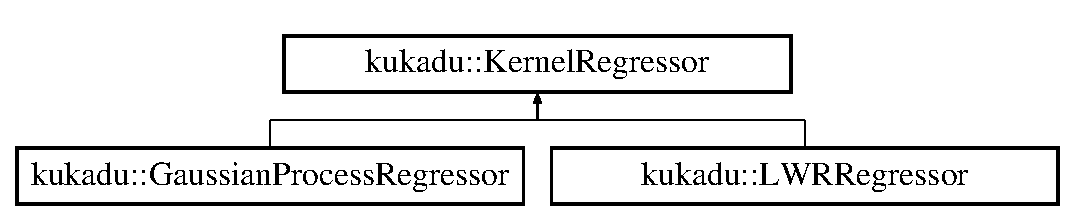
\includegraphics[height=2.000000cm]{classkukadu_1_1KernelRegressor}
\end{center}
\end{figure}
\subsection*{Public Member Functions}
\begin{DoxyCompactItemize}
\item 
\hypertarget{classkukadu_1_1KernelRegressor_a9b1048e4eb0cbc70797e27909f886e1a}{\hyperlink{classkukadu_1_1KernelRegressor_a9b1048e4eb0cbc70797e27909f886e1a}{Kernel\-Regressor} ()}\label{classkukadu_1_1KernelRegressor_a9b1048e4eb0cbc70797e27909f886e1a}

\begin{DoxyCompactList}\small\item\em constructor \end{DoxyCompactList}\item 
virtual arma\-::vec \hyperlink{classkukadu_1_1KernelRegressor_afd1489310e11cff4bd88390ba76c38e1}{fit\-At\-Position} (arma\-::vec pos)=0
\begin{DoxyCompactList}\small\item\em performs the kernel method for predicting the functin value at a given position \end{DoxyCompactList}\end{DoxyCompactItemize}


\subsection{Detailed Description}
Provides arbitrary interface for kernel methods. 

This class provides the interface for kernel machine learning methods such as Gaussian process regression or locally weighted regression 

\subsection{Member Function Documentation}
\hypertarget{classkukadu_1_1KernelRegressor_afd1489310e11cff4bd88390ba76c38e1}{\index{kukadu\-::\-Kernel\-Regressor@{kukadu\-::\-Kernel\-Regressor}!fit\-At\-Position@{fit\-At\-Position}}
\index{fit\-At\-Position@{fit\-At\-Position}!kukadu::KernelRegressor@{kukadu\-::\-Kernel\-Regressor}}
\subsubsection[{fit\-At\-Position}]{\setlength{\rightskip}{0pt plus 5cm}virtual arma\-::vec kukadu\-::\-Kernel\-Regressor\-::fit\-At\-Position (
\begin{DoxyParamCaption}
\item[{arma\-::vec}]{pos}
\end{DoxyParamCaption}
)\hspace{0.3cm}{\ttfamily [pure virtual]}}}\label{classkukadu_1_1KernelRegressor_afd1489310e11cff4bd88390ba76c38e1}


performs the kernel method for predicting the functin value at a given position 


\begin{DoxyParams}{Parameters}
{\em pos} & vector defining the required position \\
\hline
\end{DoxyParams}


Implemented in \hyperlink{classkukadu_1_1LWRRegressor_ae7d3e23243abefbfd47677967b60918b}{kukadu\-::\-L\-W\-R\-Regressor}, and \hyperlink{classkukadu_1_1GaussianProcessRegressor_a397a1d055761ae22ec9edc3d311949ec}{kukadu\-::\-Gaussian\-Process\-Regressor}.



The documentation for this class was generated from the following files\-:\begin{DoxyCompactItemize}
\item 
/home/c7031109/iis\-\_\-robot\-\_\-sw/iis\-\_\-catkin\-\_\-ws/src/kukadu/include/kukadu/learning/regression/kernelregressor.\-hpp\item 
/home/c7031109/iis\-\_\-robot\-\_\-sw/iis\-\_\-catkin\-\_\-ws/src/kukadu/src/learning/kernelregressor.\-cpp\end{DoxyCompactItemize}

\hypertarget{classkukadu_1_1Kinect}{\section{kukadu\-:\-:Kinect Class Reference}
\label{classkukadu_1_1Kinect}\index{kukadu\-::\-Kinect@{kukadu\-::\-Kinect}}
}
\subsection*{Public Member Functions}
\begin{DoxyCompactItemize}
\item 
\hypertarget{classkukadu_1_1Kinect_aa876f2bcbfe9e3b86b26805fd2275f92}{{\bfseries Kinect} (ros\-::\-Node\-Handle node)}\label{classkukadu_1_1Kinect_aa876f2bcbfe9e3b86b26805fd2275f92}

\item 
\hypertarget{classkukadu_1_1Kinect_a7c31585a1d1d6060f6028da75b31e4dd}{{\bfseries Kinect} (std\-::string kinect\-Prefix, ros\-::\-Node\-Handle node)}\label{classkukadu_1_1Kinect_a7c31585a1d1d6060f6028da75b31e4dd}

\item 
\hypertarget{classkukadu_1_1Kinect_a62836f11aa0491e7bf2317df0d7c709f}{{\bfseries Kinect} (std\-::string kinect\-Prefix, std\-::string target\-Frame, ros\-::\-Node\-Handle node)}\label{classkukadu_1_1Kinect_a62836f11aa0491e7bf2317df0d7c709f}

\item 
\hypertarget{classkukadu_1_1Kinect_aa8f05b757c4a42a25a9cc578451a823d}{void {\bfseries stop\-Sensing} ()}\label{classkukadu_1_1Kinect_aa8f05b757c4a42a25a9cc578451a823d}

\item 
\hypertarget{classkukadu_1_1Kinect_aa8041a511f9343ead3b7d1d4c889bc58}{void {\bfseries visualize\-Current\-Pc} ()}\label{classkukadu_1_1Kinect_aa8041a511f9343ead3b7d1d4c889bc58}

\item 
\hypertarget{classkukadu_1_1Kinect_a9031c091eb4e7a4400adb5a103d372fa}{void {\bfseries store\-Current\-Pc} (std\-::string file\-Name)}\label{classkukadu_1_1Kinect_a9031c091eb4e7a4400adb5a103d372fa}

\item 
\hypertarget{classkukadu_1_1Kinect_a3369fd48304d308426052f8567139589}{void {\bfseries set\-Vis\-Pub\-Topic} (std\-::string vis\-Pub\-Topic)}\label{classkukadu_1_1Kinect_a3369fd48304d308426052f8567139589}

\item 
\hypertarget{classkukadu_1_1Kinect_aa944fc517785fb7016b21c3702647561}{void {\bfseries visualize\-Current\-Transformed\-Pc} (K\-U\-K\-A\-D\-U\-\_\-\-S\-H\-A\-R\-E\-D\-\_\-\-P\-T\-R$<$ \hyperlink{classPCTransformator}{P\-C\-Transformator} $>$ transformator)}\label{classkukadu_1_1Kinect_aa944fc517785fb7016b21c3702647561}

\item 
\hypertarget{classkukadu_1_1Kinect_a7ae4121c9bb011af3d3c7f46165959e2}{bool {\bfseries is\-Initialized} ()}\label{classkukadu_1_1Kinect_a7ae4121c9bb011af3d3c7f46165959e2}

\item 
\hypertarget{classkukadu_1_1Kinect_a52f8d2b28a3b994500a5786e3dba5cab}{std\-::string {\bfseries get\-Vis\-Pub\-Topic} ()}\label{classkukadu_1_1Kinect_a52f8d2b28a3b994500a5786e3dba5cab}

\item 
\hypertarget{classkukadu_1_1Kinect_a6fb5ba75135ca2744473642a9798df67}{sensor\-\_\-msgs\-::\-Point\-Cloud2 {\bfseries get\-Current\-Point\-Cloud} ()}\label{classkukadu_1_1Kinect_a6fb5ba75135ca2744473642a9798df67}

\item 
\hypertarget{classkukadu_1_1Kinect_accb63ddb5e6024124d575e7fe229c429}{K\-U\-K\-A\-D\-U\-\_\-\-S\-H\-A\-R\-E\-D\-\_\-\-P\-T\-R$<$ kukadu\-\_\-thread $>$ {\bfseries start\-Sensing} ()}\label{classkukadu_1_1Kinect_accb63ddb5e6024124d575e7fe229c429}

\end{DoxyCompactItemize}


The documentation for this class was generated from the following files\-:\begin{DoxyCompactItemize}
\item 
/home/c7031109/iis\-\_\-robot\-\_\-sw/iis\-\_\-catkin\-\_\-ws/src/kukadu/include/kukadu/vision/kinect.\-hpp\item 
/home/c7031109/iis\-\_\-robot\-\_\-sw/iis\-\_\-catkin\-\_\-ws/src/kukadu/src/vision/kinect.\-cpp\end{DoxyCompactItemize}

\hypertarget{classkukadu_1_1Kinematics}{\section{kukadu\-:\-:Kinematics Class Reference}
\label{classkukadu_1_1Kinematics}\index{kukadu\-::\-Kinematics@{kukadu\-::\-Kinematics}}
}
Inheritance diagram for kukadu\-:\-:Kinematics\-:\begin{figure}[H]
\begin{center}
\leavevmode
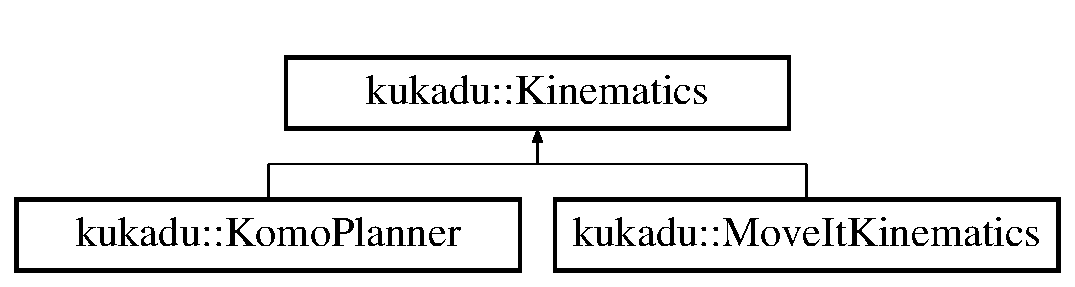
\includegraphics[height=2.000000cm]{classkukadu_1_1Kinematics}
\end{center}
\end{figure}
\subsection*{Public Member Functions}
\begin{DoxyCompactItemize}
\item 
\hypertarget{classkukadu_1_1Kinematics_af6a06ce0d0a1170148de4e8efcbbfa4b}{void {\bfseries add\-Constraint} (K\-U\-K\-A\-D\-U\-\_\-\-S\-H\-A\-R\-E\-D\-\_\-\-P\-T\-R$<$ \hyperlink{classkukadu_1_1Constraint}{Constraint} $>$ \hyperlink{classkukadu_1_1Constraint}{Constraint})}\label{classkukadu_1_1Kinematics_af6a06ce0d0a1170148de4e8efcbbfa4b}

\item 
\hypertarget{classkukadu_1_1Kinematics_a53ec74274ab1b0fd3df081a16ca35926}{void {\bfseries remove\-Constraint} (K\-U\-K\-A\-D\-U\-\_\-\-S\-H\-A\-R\-E\-D\-\_\-\-P\-T\-R$<$ \hyperlink{classkukadu_1_1Constraint}{Constraint} $>$ \hyperlink{classkukadu_1_1Constraint}{Constraint})}\label{classkukadu_1_1Kinematics_a53ec74274ab1b0fd3df081a16ca35926}

\item 
\hypertarget{classkukadu_1_1Kinematics_a4eb2b717f47bf4d28a82bfded60f75b6}{int {\bfseries get\-Constraints\-Count} ()}\label{classkukadu_1_1Kinematics_a4eb2b717f47bf4d28a82bfded60f75b6}

\item 
\hypertarget{classkukadu_1_1Kinematics_a99b99eaa016107fb4b0d8f6f87396a65}{int {\bfseries get\-Constraint\-Idx} (K\-U\-K\-A\-D\-U\-\_\-\-S\-H\-A\-R\-E\-D\-\_\-\-P\-T\-R$<$ \hyperlink{classkukadu_1_1Constraint}{Constraint} $>$ \hyperlink{classkukadu_1_1Constraint}{Constraint})}\label{classkukadu_1_1Kinematics_a99b99eaa016107fb4b0d8f6f87396a65}

\item 
\hypertarget{classkukadu_1_1Kinematics_a59ed85e60fb4d6b82bc5e145a55b1e56}{K\-U\-K\-A\-D\-U\-\_\-\-S\-H\-A\-R\-E\-D\-\_\-\-P\-T\-R$<$ \hyperlink{classkukadu_1_1Constraint}{Constraint} $>$ {\bfseries get\-Constraint\-By\-Idx} (int idx)}\label{classkukadu_1_1Kinematics_a59ed85e60fb4d6b82bc5e145a55b1e56}

\item 
\hypertarget{classkukadu_1_1Kinematics_a685f76d61feec05ba02fb8f82c30bc63}{bool {\bfseries check\-All\-Constraints} (arma\-::vec current\-State, geometry\-\_\-msgs\-::\-Pose pose)}\label{classkukadu_1_1Kinematics_a685f76d61feec05ba02fb8f82c30bc63}

\item 
\hypertarget{classkukadu_1_1Kinematics_ac9215d036bbdfab163745ade3033910e}{virtual std\-::vector$<$ arma\-::vec $>$ {\bfseries compute\-Ik} (arma\-::vec current\-Joint\-State, const geometry\-\_\-msgs\-::\-Pose \&goal)}\label{classkukadu_1_1Kinematics_ac9215d036bbdfab163745ade3033910e}

\item 
\hypertarget{classkukadu_1_1Kinematics_a5b143f7db7a84d7caa03419043426a5e}{virtual std\-::vector$<$ arma\-::vec $>$ {\bfseries compute\-Ik} (std\-::vector$<$ double $>$ current\-Joint\-State, const geometry\-\_\-msgs\-::\-Pose \&goal)=0}\label{classkukadu_1_1Kinematics_a5b143f7db7a84d7caa03419043426a5e}

\item 
\hypertarget{classkukadu_1_1Kinematics_aa80b36c16d23f6031f9b133ed72795f2}{virtual geometry\-\_\-msgs\-::\-Pose {\bfseries compute\-Fk} (std\-::vector$<$ double $>$ joint\-State)=0}\label{classkukadu_1_1Kinematics_aa80b36c16d23f6031f9b133ed72795f2}

\end{DoxyCompactItemize}


The documentation for this class was generated from the following files\-:\begin{DoxyCompactItemize}
\item 
/home/c7031109/iis\-\_\-robot\-\_\-sw/iis\-\_\-catkin\-\_\-ws/src/kukadu/include/kukadu/kinematics/kinematics.\-hpp\item 
/home/c7031109/iis\-\_\-robot\-\_\-sw/iis\-\_\-catkin\-\_\-ws/src/kukadu/src/kinematics/kinematics.\-cpp\end{DoxyCompactItemize}

\hypertarget{classkukadu_1_1KomoPlanner}{\section{kukadu\-:\-:Komo\-Planner Class Reference}
\label{classkukadu_1_1KomoPlanner}\index{kukadu\-::\-Komo\-Planner@{kukadu\-::\-Komo\-Planner}}
}
Inheritance diagram for kukadu\-:\-:Komo\-Planner\-:\begin{figure}[H]
\begin{center}
\leavevmode
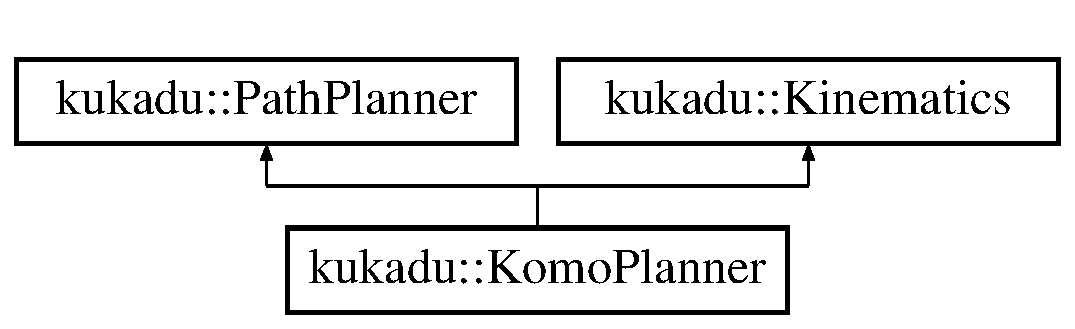
\includegraphics[height=2.000000cm]{classkukadu_1_1KomoPlanner}
\end{center}
\end{figure}
\subsection*{Public Member Functions}
\begin{DoxyCompactItemize}
\item 
\hypertarget{classkukadu_1_1KomoPlanner_a4331523418d0c7d897b9cf27402d802d}{{\bfseries Komo\-Planner} (K\-U\-K\-A\-D\-U\-\_\-\-S\-H\-A\-R\-E\-D\-\_\-\-P\-T\-R$<$ \hyperlink{classkukadu_1_1ControlQueue}{Control\-Queue} $>$ queue, std\-::string config\-Path, std\-::string mt\-Config\-Path, std\-::string active\-Joints\-Prefix, bool accept\-Collision=false)}\label{classkukadu_1_1KomoPlanner_a4331523418d0c7d897b9cf27402d802d}

\item 
\hypertarget{classkukadu_1_1KomoPlanner_a4ae46be913930cca3fb9b50af46bf5f9}{virtual std\-::vector$<$ arma\-::vec $>$ {\bfseries plan\-Joint\-Trajectory} (std\-::vector$<$ arma\-::vec $>$ intermediate\-Joints)}\label{classkukadu_1_1KomoPlanner_a4ae46be913930cca3fb9b50af46bf5f9}

\item 
\hypertarget{classkukadu_1_1KomoPlanner_a709b980d12b45751d703f5eb2209d0e9}{virtual std\-::vector$<$ arma\-::vec $>$ {\bfseries plan\-Cartesian\-Trajectory} (std\-::vector$<$ geometry\-\_\-msgs\-::\-Pose $>$ intermediate\-Poses, bool smooth\-Cartesians=false, bool use\-Current\-Robot\-State=true)}\label{classkukadu_1_1KomoPlanner_a709b980d12b45751d703f5eb2209d0e9}

\item 
\hypertarget{classkukadu_1_1KomoPlanner_a10a2433bfb06c96d93d98c9b9cff075f}{virtual std\-::vector$<$ arma\-::vec $>$ {\bfseries plan\-Cartesian\-Trajectory} (arma\-::vec start\-Joints, std\-::vector$<$ geometry\-\_\-msgs\-::\-Pose $>$ intermediate\-Poses, bool smooth\-Cartesians=false, bool use\-Current\-Robot\-State=true)}\label{classkukadu_1_1KomoPlanner_a10a2433bfb06c96d93d98c9b9cff075f}

\item 
\hypertarget{classkukadu_1_1KomoPlanner_acea4864abb57deaa9007107b65c27198}{geometry\-\_\-msgs\-::\-Pose {\bfseries compute\-Fk} (arma\-::vec joints)}\label{classkukadu_1_1KomoPlanner_acea4864abb57deaa9007107b65c27198}

\item 
\hypertarget{classkukadu_1_1KomoPlanner_ab6272ef16fa277af8b517ef3f97da658}{virtual geometry\-\_\-msgs\-::\-Pose {\bfseries compute\-Fk} (std\-::vector$<$ double $>$ joint\-State)}\label{classkukadu_1_1KomoPlanner_ab6272ef16fa277af8b517ef3f97da658}

\item 
\hypertarget{classkukadu_1_1KomoPlanner_a87a2fbfd3652e6147366b2a312f26a4e}{virtual std\-::vector$<$ arma\-::vec $>$ {\bfseries compute\-Ik} (std\-::vector$<$ double $>$ current\-Joint\-State, const geometry\-\_\-msgs\-::\-Pose \&goal)}\label{classkukadu_1_1KomoPlanner_a87a2fbfd3652e6147366b2a312f26a4e}

\end{DoxyCompactItemize}
\subsection*{Additional Inherited Members}


The documentation for this class was generated from the following files\-:\begin{DoxyCompactItemize}
\item 
/home/c7031109/iis\-\_\-robot\-\_\-sw/iis\-\_\-catkin\-\_\-ws/src/kukadu/include/kukadu/kinematics/komoplanner.\-hpp\item 
/home/c7031109/iis\-\_\-robot\-\_\-sw/iis\-\_\-catkin\-\_\-ws/src/kukadu/src/kinematics/komoplanner.\-cpp\end{DoxyCompactItemize}

\hypertarget{classKukaduException}{\section{Kukadu\-Exception Class Reference}
\label{classKukaduException}\index{Kukadu\-Exception@{Kukadu\-Exception}}
}
Inheritance diagram for Kukadu\-Exception\-:\begin{figure}[H]
\begin{center}
\leavevmode
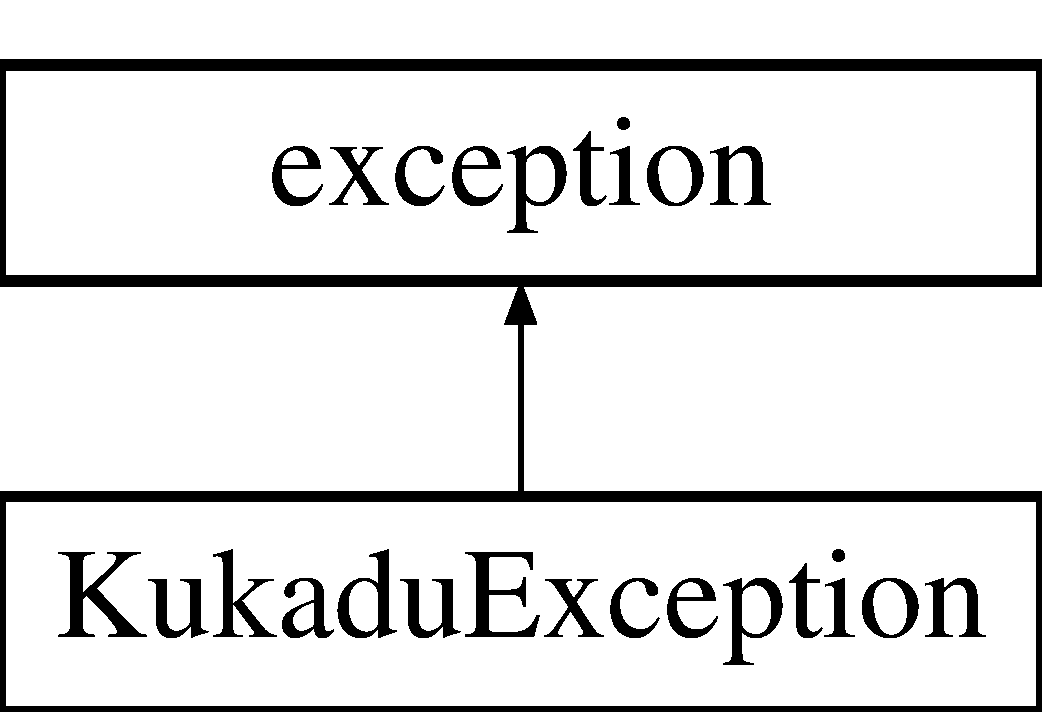
\includegraphics[height=2.000000cm]{classKukaduException}
\end{center}
\end{figure}
\subsection*{Public Member Functions}
\begin{DoxyCompactItemize}
\item 
\hypertarget{classKukaduException_a42b9f7e8168faec423147a324a9da6a8}{{\bfseries Kukadu\-Exception} (const char $\ast$message)}\label{classKukaduException_a42b9f7e8168faec423147a324a9da6a8}

\item 
\hypertarget{classKukaduException_ad5113f32aacb509bf29c9e3e8288b2f5}{virtual const char $\ast$ {\bfseries what} () const   throw ()}\label{classKukaduException_ad5113f32aacb509bf29c9e3e8288b2f5}

\end{DoxyCompactItemize}


The documentation for this class was generated from the following file\-:\begin{DoxyCompactItemize}
\item 
/home/c7031109/iis\-\_\-robot\-\_\-sw/iis\-\_\-catkin\-\_\-ws/src/kukadu/include/kukadu/types/kukadutypes.\-hpp\end{DoxyCompactItemize}

\hypertarget{classkukadu_1_1KukaduTokenizer}{\section{kukadu\-:\-:Kukadu\-Tokenizer Class Reference}
\label{classkukadu_1_1KukaduTokenizer}\index{kukadu\-::\-Kukadu\-Tokenizer@{kukadu\-::\-Kukadu\-Tokenizer}}
}
\subsection*{Public Member Functions}
\begin{DoxyCompactItemize}
\item 
\hypertarget{classkukadu_1_1KukaduTokenizer_aae8ae3c9b1fa4cf3b2e1d7aacce89042}{{\bfseries Kukadu\-Tokenizer} (const std\-::string \&str, const std\-::string \&delimiter=D\-E\-F\-A\-U\-L\-T\-\_\-\-D\-E\-L\-I\-M\-I\-T\-E\-R)}\label{classkukadu_1_1KukaduTokenizer_aae8ae3c9b1fa4cf3b2e1d7aacce89042}

\item 
\hypertarget{classkukadu_1_1KukaduTokenizer_a0bf607b688bdb8a21371335ac4415a1e}{void {\bfseries set} (const std\-::string \&str, const std\-::string \&delimiter=D\-E\-F\-A\-U\-L\-T\-\_\-\-D\-E\-L\-I\-M\-I\-T\-E\-R)}\label{classkukadu_1_1KukaduTokenizer_a0bf607b688bdb8a21371335ac4415a1e}

\item 
\hypertarget{classkukadu_1_1KukaduTokenizer_a0d3d6891c51dff67d9b9b367f9ffc930}{void {\bfseries set\-String} (const std\-::string \&str)}\label{classkukadu_1_1KukaduTokenizer_a0d3d6891c51dff67d9b9b367f9ffc930}

\item 
\hypertarget{classkukadu_1_1KukaduTokenizer_a6ca4375a16e6be13c2b425345c324811}{void {\bfseries set\-Delimiter} (const std\-::string \&delimiter)}\label{classkukadu_1_1KukaduTokenizer_a6ca4375a16e6be13c2b425345c324811}

\item 
\hypertarget{classkukadu_1_1KukaduTokenizer_a1276cdd662e68254f9f7f277e534603d}{std\-::string {\bfseries next} ()}\label{classkukadu_1_1KukaduTokenizer_a1276cdd662e68254f9f7f277e534603d}

\item 
\hypertarget{classkukadu_1_1KukaduTokenizer_ac432b19d37cd0ee3baf73d7ee350cf55}{void {\bfseries put\-Back\-Last} ()}\label{classkukadu_1_1KukaduTokenizer_ac432b19d37cd0ee3baf73d7ee350cf55}

\item 
\hypertarget{classkukadu_1_1KukaduTokenizer_a8fa96ce320c74d7b350546c28bc18d12}{std\-::vector$<$ std\-::string $>$ {\bfseries split} ()}\label{classkukadu_1_1KukaduTokenizer_a8fa96ce320c74d7b350546c28bc18d12}

\item 
\hypertarget{classkukadu_1_1KukaduTokenizer_a4d9ef340611b923b365394ee314f05b3}{int {\bfseries get\-Token\-Idx} ()}\label{classkukadu_1_1KukaduTokenizer_a4d9ef340611b923b365394ee314f05b3}

\end{DoxyCompactItemize}


The documentation for this class was generated from the following files\-:\begin{DoxyCompactItemize}
\item 
/home/c7031109/iis\-\_\-robot\-\_\-sw/iis\-\_\-catkin\-\_\-ws/src/kukadu/include/kukadu/utils/kukadutokenizer.\-hpp\item 
/home/c7031109/iis\-\_\-robot\-\_\-sw/iis\-\_\-catkin\-\_\-ws/src/kukadu/src/utils/kukadutokenizer.\-cpp\end{DoxyCompactItemize}

\hypertarget{classkukadu_1_1KukieControlQueue}{\section{kukadu\-:\-:Kukie\-Control\-Queue Class Reference}
\label{classkukadu_1_1KukieControlQueue}\index{kukadu\-::\-Kukie\-Control\-Queue@{kukadu\-::\-Kukie\-Control\-Queue}}
}


Contains an implementation of the control queue interface for robots supporting the I\-I\-S\-Kukie system. This interface is responsible for all communication the kukadu software stack and the robotic arm.  




{\ttfamily \#include $<$kukiecontrolqueue.\-hpp$>$}

Inheritance diagram for kukadu\-:\-:Kukie\-Control\-Queue\-:\begin{figure}[H]
\begin{center}
\leavevmode
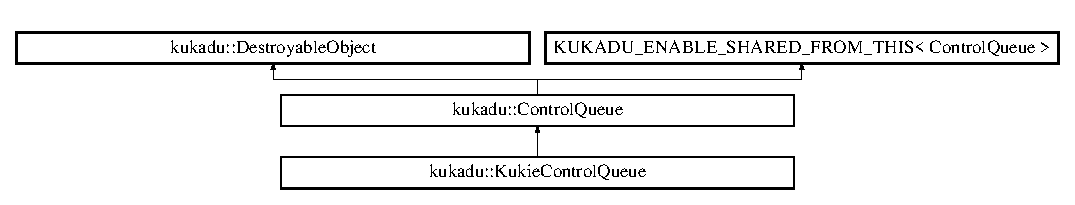
\includegraphics[height=2.301370cm]{classkukadu_1_1KukieControlQueue}
\end{center}
\end{figure}
\subsection*{Public Member Functions}
\begin{DoxyCompactItemize}
\item 
\hypertarget{classkukadu_1_1KukieControlQueue_af8995cf0a8a9e1d5a77d296af0e94b3a}{{\bfseries Kukie\-Control\-Queue} (std\-::string device\-Type, std\-::string arm\-Prefix, ros\-::\-Node\-Handle node, bool accept\-Collisions=false, K\-U\-K\-A\-D\-U\-\_\-\-S\-H\-A\-R\-E\-D\-\_\-\-P\-T\-R$<$ \hyperlink{classkukadu_1_1Kinematics}{Kinematics} $>$ kin=K\-U\-K\-A\-D\-U\-\_\-\-S\-H\-A\-R\-E\-D\-\_\-\-P\-T\-R$<$ \hyperlink{classkukadu_1_1Kinematics}{Kinematics} $>$(), K\-U\-K\-A\-D\-U\-\_\-\-S\-H\-A\-R\-E\-D\-\_\-\-P\-T\-R$<$ \hyperlink{classkukadu_1_1PathPlanner}{Path\-Planner} $>$ planner=K\-U\-K\-A\-D\-U\-\_\-\-S\-H\-A\-R\-E\-D\-\_\-\-P\-T\-R$<$ \hyperlink{classkukadu_1_1PathPlanner}{Path\-Planner} $>$(), double sleep\-Time=-\/1.\-0, double max\-Dist\-Per\-Cycle=-\/1.\-0)}\label{classkukadu_1_1KukieControlQueue_af8995cf0a8a9e1d5a77d296af0e94b3a}

\item 
void \hyperlink{classkukadu_1_1KukieControlQueue_a39da1e622d39d7870c9d0e802d5afa4b}{safely\-Destroy} ()
\begin{DoxyCompactList}\small\item\em Method is called whenever destroy event occurs and ensures safe and clean termination of the programm (e.\-g. stops robot) \end{DoxyCompactList}\item 
\hypertarget{classkukadu_1_1KukieControlQueue_a0e8516eeb18eabfe472ef2552adb5855}{void {\bfseries set\-Kinematics} (K\-U\-K\-A\-D\-U\-\_\-\-S\-H\-A\-R\-E\-D\-\_\-\-P\-T\-R$<$ \hyperlink{classkukadu_1_1Kinematics}{Kinematics} $>$ kin)}\label{classkukadu_1_1KukieControlQueue_a0e8516eeb18eabfe472ef2552adb5855}

\item 
\hypertarget{classkukadu_1_1KukieControlQueue_ae4fed3b50bbe1ea52be8ee5b0c327462}{void {\bfseries set\-Path\-Planner} (K\-U\-K\-A\-D\-U\-\_\-\-S\-H\-A\-R\-E\-D\-\_\-\-P\-T\-R$<$ \hyperlink{classkukadu_1_1PathPlanner}{Path\-Planner} $>$ planner)}\label{classkukadu_1_1KukieControlQueue_ae4fed3b50bbe1ea52be8ee5b0c327462}

\item 
void \hyperlink{classkukadu_1_1KukieControlQueue_ac6653c3a050bb338702294776b4a8065}{set\-Jnt\-Ptp\-Thresh} (double thresh)
\begin{DoxyCompactList}\small\item\em Sets the maximum deviation in joint space that is tolerated for a point to point movement. \end{DoxyCompactList}\item 
void \hyperlink{classkukadu_1_1KukieControlQueue_a0fef688170ac5a3e21df426a30ef0e77}{set\-Additional\-Load} (float load\-Mass, float load\-Pos)
\begin{DoxyCompactList}\small\item\em Changes the expected load data of the robot (e.\-g. can be used whenever robot picks up an object). Some robots might require this information in order to avoid control problems. \end{DoxyCompactList}\item 
void \hyperlink{classkukadu_1_1KukieControlQueue_a3145cfcb1dc4879e2e3f16ad4829ce09}{set\-Stiffness} (float cpstiffnessxyz, float cpstiffnessabc, float cpdamping, float cpmaxdelta, float maxforce, float axismaxdeltatrq)
\begin{DoxyCompactList}\small\item\em Sets certain stiffness parameters in cartesian space (if the robot supports this) according to a mass spring damper system model. \end{DoxyCompactList}\item 
int \hyperlink{classkukadu_1_1KukieControlQueue_aecd7cca5bf0b7dd990d061acdee56ce3}{get\-Current\-Mode} ()
\begin{DoxyCompactList}\small\item\em Returns the current robot control mode (see \hyperlink{classkukadu_1_1ControlQueue_a5defe63d9f1b9829676f9a31a4683911}{switch\-Mode()}) \end{DoxyCompactList}\item 
std\-::string \hyperlink{classkukadu_1_1KukieControlQueue_aa1edc1807aad2cf5f991c0a70fb2bc40}{get\-Robot\-Name} ()
\begin{DoxyCompactList}\small\item\em Returns the robot name. \end{DoxyCompactList}\item 
std\-::string \hyperlink{classkukadu_1_1KukieControlQueue_a390da7a21b5c9f42ceff914155499b76}{get\-Robot\-File\-Name} ()
\begin{DoxyCompactList}\small\item\em Returns the robot name with escaped special characaters (e.\-g. white spaces) \end{DoxyCompactList}\item 
\hypertarget{classkukadu_1_1KukieControlQueue_abab099320e0d9f4f6d68c784fcbfeb15}{std\-::string {\bfseries get\-Robot\-Side\-Prefix} ()}\label{classkukadu_1_1KukieControlQueue_abab099320e0d9f4f6d68c784fcbfeb15}

\item 
\hypertarget{classkukadu_1_1KukieControlQueue_ad62cd51305bd1ac8b5da9629b7f3116f}{std\-::string {\bfseries get\-Robot\-Device\-Type} ()}\label{classkukadu_1_1KukieControlQueue_ad62cd51305bd1ac8b5da9629b7f3116f}

\item 
std\-::vector$<$ std\-::string $>$ \hyperlink{classkukadu_1_1KukieControlQueue_af3c7ff340cd44a44233c209eeed9d929}{get\-Joint\-Names} ()
\begin{DoxyCompactList}\small\item\em Returns the robot joint names. \end{DoxyCompactList}\item 
\hyperlink{structmes__result}{mes\-\_\-result} \hyperlink{classkukadu_1_1KukieControlQueue_aecf704318e729f49999d3be51262f068}{get\-Current\-Joints} ()
\begin{DoxyCompactList}\small\item\em Returns joints if the robot is in command mode. \end{DoxyCompactList}\item 
\hyperlink{structmes__result}{mes\-\_\-result} \hyperlink{classkukadu_1_1KukieControlQueue_a947d5f2d42060bdd6d7271d80ac40e7a}{get\-Current\-Jnt\-Frc} ()
\begin{DoxyCompactList}\small\item\em Returns the forces measured for the robot joints. \end{DoxyCompactList}\item 
\hyperlink{structmes__result}{mes\-\_\-result} \hyperlink{classkukadu_1_1KukieControlQueue_af9999c0af6059520452f0d42a8db4527}{get\-Current\-Cartesian\-Frc\-Trq} ()
\begin{DoxyCompactList}\small\item\em Returns the forces and torques measured at the robot end-\/effector. \end{DoxyCompactList}\item 
geometry\-\_\-msgs\-::\-Pose \hyperlink{classkukadu_1_1KukieControlQueue_ab13290e3512b3a1ab10660b0f60e6961}{get\-Current\-Cartesian\-Pose} ()
\begin{DoxyCompactList}\small\item\em Returns current robot position in cartesian space. \end{DoxyCompactList}\item 
\hypertarget{classkukadu_1_1KukieControlQueue_a4ecef16deac6daa191d942cf00526550}{geometry\-\_\-msgs\-::\-Pose {\bfseries get\-Current\-Cartesian\-Pose\-Rf} ()}\label{classkukadu_1_1KukieControlQueue_a4ecef16deac6daa191d942cf00526550}

\item 
\hypertarget{classkukadu_1_1KukieControlQueue_ad0964c0cbfc3a44b7544396d5b9d0cba}{geometry\-\_\-msgs\-::\-Pose {\bfseries move\-Cartesian\-Relative\-Wf} (geometry\-\_\-msgs\-::\-Pose base\-Pose\-Rf, geometry\-\_\-msgs\-::\-Pose offset)}\label{classkukadu_1_1KukieControlQueue_ad0964c0cbfc3a44b7544396d5b9d0cba}

\item 
\hypertarget{classkukadu_1_1KukieControlQueue_ab6563d18842c941f87ae942c983e47bd}{arma\-::vec {\bfseries get\-Frc\-Trq\-Cart} ()}\label{classkukadu_1_1KukieControlQueue_ab6563d18842c941f87ae942c983e47bd}

\item 
\hypertarget{classkukadu_1_1KukieControlQueue_aeab6a219bc62aca73cdbac872a8aad7c}{K\-U\-K\-A\-D\-U\-\_\-\-S\-H\-A\-R\-E\-D\-\_\-\-P\-T\-R$<$ \hyperlink{classkukadu_1_1Kinematics}{Kinematics} $>$ {\bfseries get\-Kinematics} ()}\label{classkukadu_1_1KukieControlQueue_aeab6a219bc62aca73cdbac872a8aad7c}

\end{DoxyCompactItemize}
\subsection*{Static Public Attributes}
\begin{DoxyCompactItemize}
\item 
\hypertarget{classkukadu_1_1KukieControlQueue_a8dd833cde832e46a18cff94c5d7b6178}{static const int {\bfseries K\-U\-K\-A\-\_\-\-S\-T\-O\-P\-\_\-\-M\-O\-D\-E} = 0}\label{classkukadu_1_1KukieControlQueue_a8dd833cde832e46a18cff94c5d7b6178}

\item 
\hypertarget{classkukadu_1_1KukieControlQueue_a0be0d5939cfa6de326762e2689f1e0b3}{static const int {\bfseries K\-U\-K\-A\-\_\-\-J\-N\-T\-\_\-\-P\-O\-S\-\_\-\-M\-O\-D\-E} = 10}\label{classkukadu_1_1KukieControlQueue_a0be0d5939cfa6de326762e2689f1e0b3}

\item 
\hypertarget{classkukadu_1_1KukieControlQueue_af6dc1a4a6d11223b8384e3bdfad713e7}{static const int {\bfseries K\-U\-K\-A\-\_\-\-C\-A\-R\-T\-\_\-\-I\-M\-P\-\_\-\-M\-O\-D\-E} = 20}\label{classkukadu_1_1KukieControlQueue_af6dc1a4a6d11223b8384e3bdfad713e7}

\item 
\hypertarget{classkukadu_1_1KukieControlQueue_a821a4327dd8d02a6e5bb914d8fb0a4f2}{static const int {\bfseries K\-U\-K\-A\-\_\-\-J\-N\-T\-\_\-\-I\-M\-P\-\_\-\-M\-O\-D\-E} = 30}\label{classkukadu_1_1KukieControlQueue_a821a4327dd8d02a6e5bb914d8fb0a4f2}

\item 
\hypertarget{classkukadu_1_1KukieControlQueue_a4f36537e3f8d3968cd36460741f83ec3}{static const int {\bfseries K\-U\-K\-A\-\_\-\-S\-T\-D\-\_\-\-X\-Y\-Z\-\_\-\-S\-T\-I\-F\-F} = 250}\label{classkukadu_1_1KukieControlQueue_a4f36537e3f8d3968cd36460741f83ec3}

\item 
\hypertarget{classkukadu_1_1KukieControlQueue_a803666b1c82d70b7b84b05cedd5e4340}{static const int {\bfseries K\-U\-K\-A\-\_\-\-S\-T\-D\-\_\-\-A\-B\-C\-\_\-\-S\-T\-I\-F\-F} = 100}\label{classkukadu_1_1KukieControlQueue_a803666b1c82d70b7b84b05cedd5e4340}

\item 
\hypertarget{classkukadu_1_1KukieControlQueue_a1b73e604f852fe832da9016105a02c7c}{static const int {\bfseries K\-U\-K\-A\-\_\-\-S\-T\-D\-\_\-\-C\-P\-D\-A\-M\-P\-I\-N\-G} = 0.\-3}\label{classkukadu_1_1KukieControlQueue_a1b73e604f852fe832da9016105a02c7c}

\end{DoxyCompactItemize}
\subsection*{Protected Member Functions}
\begin{DoxyCompactItemize}
\item 
\hypertarget{classkukadu_1_1KukieControlQueue_ab828e3291b59e05855efd323a0124ac4}{virtual void \hyperlink{classkukadu_1_1KukieControlQueue_ab828e3291b59e05855efd323a0124ac4}{set\-Init\-Values} ()}\label{classkukadu_1_1KukieControlQueue_ab828e3291b59e05855efd323a0124ac4}

\begin{DoxyCompactList}\small\item\em This method can be used to initialize custom parts of the \hyperlink{classkukadu_1_1ControlQueue}{Control\-Queue} implementation before the queue is started by \hyperlink{classkukadu_1_1ControlQueue_a35d6a6e4e7c8467691c11567fe21f340}{start\-Queue()}. \end{DoxyCompactList}\item 
\hypertarget{classkukadu_1_1KukieControlQueue_ab86936efc30e3b3584fdaf98ef006540}{virtual void \hyperlink{classkukadu_1_1KukieControlQueue_ab86936efc30e3b3584fdaf98ef006540}{start\-Queue\-Hook} ()}\label{classkukadu_1_1KukieControlQueue_ab86936efc30e3b3584fdaf98ef006540}

\begin{DoxyCompactList}\small\item\em This method can be used to add some additional initialization behavior when the queue is started. If no additional initialization is required, the method can be left empty. \end{DoxyCompactList}\item 
\hypertarget{classkukadu_1_1KukieControlQueue_a73687ba516b2cfb5f9124ae9f165fc57}{virtual void \hyperlink{classkukadu_1_1KukieControlQueue_a73687ba516b2cfb5f9124ae9f165fc57}{joint\-Ptp\-Internal} (arma\-::vec joints)}\label{classkukadu_1_1KukieControlQueue_a73687ba516b2cfb5f9124ae9f165fc57}

\begin{DoxyCompactList}\small\item\em The control queue collects the data about the actually executed trajectory during a point to point movement. This is automatically done by \hyperlink{classkukadu_1_1ControlQueue_ad11059100321b24a1af8ef7de8314353}{joint\-Ptp()}. \hyperlink{classkukadu_1_1ControlQueue_ad11059100321b24a1af8ef7de8314353}{joint\-Ptp()} calls the \hyperlink{classkukadu_1_1KukieControlQueue_a73687ba516b2cfb5f9124ae9f165fc57}{joint\-Ptp\-Internal()} function that actually plans the movement in joint space and executes it. \end{DoxyCompactList}\item 
\hypertarget{classkukadu_1_1KukieControlQueue_a801f4d00e4eed9c11a53cb1521db42f0}{virtual void \hyperlink{classkukadu_1_1KukieControlQueue_a801f4d00e4eed9c11a53cb1521db42f0}{submit\-Next\-Joint\-Move} (arma\-::vec joints)}\label{classkukadu_1_1KukieControlQueue_a801f4d00e4eed9c11a53cb1521db42f0}

\begin{DoxyCompactList}\small\item\em This method is called by the run() method once per clock cycle and actually submits the command about the next desired joint pose to the robot. \end{DoxyCompactList}\item 
\hypertarget{classkukadu_1_1KukieControlQueue_af5ae9a7107d58e35f340f24fcb3785db}{virtual void \hyperlink{classkukadu_1_1KukieControlQueue_af5ae9a7107d58e35f340f24fcb3785db}{cart\-Ptp\-Internal} (geometry\-\_\-msgs\-::\-Pose pos, double max\-Force)}\label{classkukadu_1_1KukieControlQueue_af5ae9a7107d58e35f340f24fcb3785db}

\begin{DoxyCompactList}\small\item\em The control queue collects the data about the actually executed trajectory during a point to point movement. This is automatically done by \hyperlink{classkukadu_1_1ControlQueue_a1bfa23a8ce6319f6ef0ed9208e896054}{cartesian\-Ptp()}. \hyperlink{classkukadu_1_1ControlQueue_a1bfa23a8ce6319f6ef0ed9208e896054}{cartesian\-Ptp()} calls the \hyperlink{classkukadu_1_1KukieControlQueue_af5ae9a7107d58e35f340f24fcb3785db}{cart\-Ptp\-Internal()} function that actually plans the movement in Cartesian space and executes it. \end{DoxyCompactList}\item 
\hypertarget{classkukadu_1_1KukieControlQueue_a7976aea7ef93fe9c96d017309e11e2c1}{virtual void \hyperlink{classkukadu_1_1KukieControlQueue_a7976aea7ef93fe9c96d017309e11e2c1}{submit\-Next\-Cart\-Move} (geometry\-\_\-msgs\-::\-Pose pose)}\label{classkukadu_1_1KukieControlQueue_a7976aea7ef93fe9c96d017309e11e2c1}

\begin{DoxyCompactList}\small\item\em This method is called by the run() method once per clock cycle and actually submits the command about the next desired Cartesian pose to the robot. \end{DoxyCompactList}\item 
\hypertarget{classkukadu_1_1KukieControlQueue_ade8c63d5fad6dedbbd89b1f1a8915191}{virtual void \hyperlink{classkukadu_1_1KukieControlQueue_ade8c63d5fad6dedbbd89b1f1a8915191}{set\-Current\-Control\-Type\-Internal} (int control\-Type)}\label{classkukadu_1_1KukieControlQueue_ade8c63d5fad6dedbbd89b1f1a8915191}

\begin{DoxyCompactList}\small\item\em This method is called by \hyperlink{classkukadu_1_1ControlQueue_a5defe63d9f1b9829676f9a31a4683911}{switch\-Mode()} and actually sends the control mode command to the robot. \end{DoxyCompactList}\item 
virtual bool \hyperlink{classkukadu_1_1KukieControlQueue_abb6d8763fada53c6583b2a1ef58274ed}{stop\-Queue\-While\-Ptp} ()
\begin{DoxyCompactList}\small\item\em This method determines, if the queue execetion should be stopped while ptp commands are executed (this is typically the case when ptp is done outside of the control queue implementation). If two different controls interfere it can result in dangerous behaviour. \end{DoxyCompactList}\end{DoxyCompactItemize}
\subsection*{Additional Inherited Members}


\subsection{Detailed Description}
Contains an implementation of the control queue interface for robots supporting the I\-I\-S\-Kukie system. This interface is responsible for all communication the kukadu software stack and the robotic arm. 

\subsection{Member Function Documentation}
\hypertarget{classkukadu_1_1KukieControlQueue_af9999c0af6059520452f0d42a8db4527}{\index{kukadu\-::\-Kukie\-Control\-Queue@{kukadu\-::\-Kukie\-Control\-Queue}!get\-Current\-Cartesian\-Frc\-Trq@{get\-Current\-Cartesian\-Frc\-Trq}}
\index{get\-Current\-Cartesian\-Frc\-Trq@{get\-Current\-Cartesian\-Frc\-Trq}!kukadu::KukieControlQueue@{kukadu\-::\-Kukie\-Control\-Queue}}
\subsubsection[{get\-Current\-Cartesian\-Frc\-Trq}]{\setlength{\rightskip}{0pt plus 5cm}{\bf mes\-\_\-result} kukadu\-::\-Kukie\-Control\-Queue\-::get\-Current\-Cartesian\-Frc\-Trq (
\begin{DoxyParamCaption}
{}
\end{DoxyParamCaption}
)\hspace{0.3cm}{\ttfamily [virtual]}}}\label{classkukadu_1_1KukieControlQueue_af9999c0af6059520452f0d42a8db4527}


Returns the forces and torques measured at the robot end-\/effector. 

\begin{DoxyReturn}{Returns}
The current forces and torques (in Newton and Newton / meter) 
\end{DoxyReturn}


Implements \hyperlink{classkukadu_1_1ControlQueue_aa557f386f03cfb4986ed7cd9997212ab}{kukadu\-::\-Control\-Queue}.

\hypertarget{classkukadu_1_1KukieControlQueue_ab13290e3512b3a1ab10660b0f60e6961}{\index{kukadu\-::\-Kukie\-Control\-Queue@{kukadu\-::\-Kukie\-Control\-Queue}!get\-Current\-Cartesian\-Pose@{get\-Current\-Cartesian\-Pose}}
\index{get\-Current\-Cartesian\-Pose@{get\-Current\-Cartesian\-Pose}!kukadu::KukieControlQueue@{kukadu\-::\-Kukie\-Control\-Queue}}
\subsubsection[{get\-Current\-Cartesian\-Pose}]{\setlength{\rightskip}{0pt plus 5cm}geometry\-\_\-msgs\-::\-Pose kukadu\-::\-Kukie\-Control\-Queue\-::get\-Current\-Cartesian\-Pose (
\begin{DoxyParamCaption}
{}
\end{DoxyParamCaption}
)\hspace{0.3cm}{\ttfamily [virtual]}}}\label{classkukadu_1_1KukieControlQueue_ab13290e3512b3a1ab10660b0f60e6961}


Returns current robot position in cartesian space. 

\begin{DoxyReturn}{Returns}
current pose of the robot in Cartesian space 
\end{DoxyReturn}


Implements \hyperlink{classkukadu_1_1ControlQueue_a9e79e1d0d9697bbf146d66a2d01fea9e}{kukadu\-::\-Control\-Queue}.

\hypertarget{classkukadu_1_1KukieControlQueue_a947d5f2d42060bdd6d7271d80ac40e7a}{\index{kukadu\-::\-Kukie\-Control\-Queue@{kukadu\-::\-Kukie\-Control\-Queue}!get\-Current\-Jnt\-Frc@{get\-Current\-Jnt\-Frc}}
\index{get\-Current\-Jnt\-Frc@{get\-Current\-Jnt\-Frc}!kukadu::KukieControlQueue@{kukadu\-::\-Kukie\-Control\-Queue}}
\subsubsection[{get\-Current\-Jnt\-Frc}]{\setlength{\rightskip}{0pt plus 5cm}{\bf mes\-\_\-result} kukadu\-::\-Kukie\-Control\-Queue\-::get\-Current\-Jnt\-Frc (
\begin{DoxyParamCaption}
{}
\end{DoxyParamCaption}
)\hspace{0.3cm}{\ttfamily [virtual]}}}\label{classkukadu_1_1KukieControlQueue_a947d5f2d42060bdd6d7271d80ac40e7a}


Returns the forces measured for the robot joints. 

\begin{DoxyReturn}{Returns}
The current forces measured at the robot joints (in Newton) 
\end{DoxyReturn}


Implements \hyperlink{classkukadu_1_1ControlQueue_a1468c1771ea7dfd1ee3b0a7279407241}{kukadu\-::\-Control\-Queue}.

\hypertarget{classkukadu_1_1KukieControlQueue_aecf704318e729f49999d3be51262f068}{\index{kukadu\-::\-Kukie\-Control\-Queue@{kukadu\-::\-Kukie\-Control\-Queue}!get\-Current\-Joints@{get\-Current\-Joints}}
\index{get\-Current\-Joints@{get\-Current\-Joints}!kukadu::KukieControlQueue@{kukadu\-::\-Kukie\-Control\-Queue}}
\subsubsection[{get\-Current\-Joints}]{\setlength{\rightskip}{0pt plus 5cm}{\bf mes\-\_\-result} kukadu\-::\-Kukie\-Control\-Queue\-::get\-Current\-Joints (
\begin{DoxyParamCaption}
{}
\end{DoxyParamCaption}
)\hspace{0.3cm}{\ttfamily [virtual]}}}\label{classkukadu_1_1KukieControlQueue_aecf704318e729f49999d3be51262f068}


Returns joints if the robot is in command mode. 

\begin{DoxyReturn}{Returns}
The current joint pose of the robot 
\end{DoxyReturn}


Implements \hyperlink{classkukadu_1_1ControlQueue_a6ba7b6db5099073eadd7bc04792bc643}{kukadu\-::\-Control\-Queue}.

\hypertarget{classkukadu_1_1KukieControlQueue_aecd7cca5bf0b7dd990d061acdee56ce3}{\index{kukadu\-::\-Kukie\-Control\-Queue@{kukadu\-::\-Kukie\-Control\-Queue}!get\-Current\-Mode@{get\-Current\-Mode}}
\index{get\-Current\-Mode@{get\-Current\-Mode}!kukadu::KukieControlQueue@{kukadu\-::\-Kukie\-Control\-Queue}}
\subsubsection[{get\-Current\-Mode}]{\setlength{\rightskip}{0pt plus 5cm}int kukadu\-::\-Kukie\-Control\-Queue\-::get\-Current\-Mode (
\begin{DoxyParamCaption}
{}
\end{DoxyParamCaption}
)\hspace{0.3cm}{\ttfamily [virtual]}}}\label{classkukadu_1_1KukieControlQueue_aecd7cca5bf0b7dd990d061acdee56ce3}


Returns the current robot control mode (see \hyperlink{classkukadu_1_1ControlQueue_a5defe63d9f1b9829676f9a31a4683911}{switch\-Mode()}) 

\begin{DoxyReturn}{Returns}
Current robot control mode 
\end{DoxyReturn}


Implements \hyperlink{classkukadu_1_1ControlQueue_afce92074c674d8a1b0127190fd0603cf}{kukadu\-::\-Control\-Queue}.

\hypertarget{classkukadu_1_1KukieControlQueue_af3c7ff340cd44a44233c209eeed9d929}{\index{kukadu\-::\-Kukie\-Control\-Queue@{kukadu\-::\-Kukie\-Control\-Queue}!get\-Joint\-Names@{get\-Joint\-Names}}
\index{get\-Joint\-Names@{get\-Joint\-Names}!kukadu::KukieControlQueue@{kukadu\-::\-Kukie\-Control\-Queue}}
\subsubsection[{get\-Joint\-Names}]{\setlength{\rightskip}{0pt plus 5cm}std\-::vector$<$ std\-::string $>$ kukadu\-::\-Kukie\-Control\-Queue\-::get\-Joint\-Names (
\begin{DoxyParamCaption}
{}
\end{DoxyParamCaption}
)\hspace{0.3cm}{\ttfamily [virtual]}}}\label{classkukadu_1_1KukieControlQueue_af3c7ff340cd44a44233c209eeed9d929}


Returns the robot joint names. 

\begin{DoxyReturn}{Returns}
robot joint names 
\end{DoxyReturn}


Implements \hyperlink{classkukadu_1_1ControlQueue_a85702573cb64f7f3dd9c3d2eac95a6ea}{kukadu\-::\-Control\-Queue}.

\hypertarget{classkukadu_1_1KukieControlQueue_a390da7a21b5c9f42ceff914155499b76}{\index{kukadu\-::\-Kukie\-Control\-Queue@{kukadu\-::\-Kukie\-Control\-Queue}!get\-Robot\-File\-Name@{get\-Robot\-File\-Name}}
\index{get\-Robot\-File\-Name@{get\-Robot\-File\-Name}!kukadu::KukieControlQueue@{kukadu\-::\-Kukie\-Control\-Queue}}
\subsubsection[{get\-Robot\-File\-Name}]{\setlength{\rightskip}{0pt plus 5cm}std\-::string kukadu\-::\-Kukie\-Control\-Queue\-::get\-Robot\-File\-Name (
\begin{DoxyParamCaption}
{}
\end{DoxyParamCaption}
)\hspace{0.3cm}{\ttfamily [virtual]}}}\label{classkukadu_1_1KukieControlQueue_a390da7a21b5c9f42ceff914155499b76}


Returns the robot name with escaped special characaters (e.\-g. white spaces) 

\begin{DoxyReturn}{Returns}
robot name 
\end{DoxyReturn}


Implements \hyperlink{classkukadu_1_1ControlQueue_aab7dbf0d07b829b9612cfe7141c801a1}{kukadu\-::\-Control\-Queue}.

\hypertarget{classkukadu_1_1KukieControlQueue_aa1edc1807aad2cf5f991c0a70fb2bc40}{\index{kukadu\-::\-Kukie\-Control\-Queue@{kukadu\-::\-Kukie\-Control\-Queue}!get\-Robot\-Name@{get\-Robot\-Name}}
\index{get\-Robot\-Name@{get\-Robot\-Name}!kukadu::KukieControlQueue@{kukadu\-::\-Kukie\-Control\-Queue}}
\subsubsection[{get\-Robot\-Name}]{\setlength{\rightskip}{0pt plus 5cm}std\-::string kukadu\-::\-Kukie\-Control\-Queue\-::get\-Robot\-Name (
\begin{DoxyParamCaption}
{}
\end{DoxyParamCaption}
)\hspace{0.3cm}{\ttfamily [virtual]}}}\label{classkukadu_1_1KukieControlQueue_aa1edc1807aad2cf5f991c0a70fb2bc40}


Returns the robot name. 

\begin{DoxyReturn}{Returns}
robot name 
\end{DoxyReturn}


Implements \hyperlink{classkukadu_1_1ControlQueue_aff34133be55d32e07d0ce6aac26cf10d}{kukadu\-::\-Control\-Queue}.

\hypertarget{classkukadu_1_1KukieControlQueue_a39da1e622d39d7870c9d0e802d5afa4b}{\index{kukadu\-::\-Kukie\-Control\-Queue@{kukadu\-::\-Kukie\-Control\-Queue}!safely\-Destroy@{safely\-Destroy}}
\index{safely\-Destroy@{safely\-Destroy}!kukadu::KukieControlQueue@{kukadu\-::\-Kukie\-Control\-Queue}}
\subsubsection[{safely\-Destroy}]{\setlength{\rightskip}{0pt plus 5cm}void kukadu\-::\-Kukie\-Control\-Queue\-::safely\-Destroy (
\begin{DoxyParamCaption}
{}
\end{DoxyParamCaption}
)\hspace{0.3cm}{\ttfamily [virtual]}}}\label{classkukadu_1_1KukieControlQueue_a39da1e622d39d7870c9d0e802d5afa4b}


Method is called whenever destroy event occurs and ensures safe and clean termination of the programm (e.\-g. stops robot) 



Implements \hyperlink{classkukadu_1_1DestroyableObject_a9e490cfa46af84690eb5ff0682df986c}{kukadu\-::\-Destroyable\-Object}.

\hypertarget{classkukadu_1_1KukieControlQueue_a0fef688170ac5a3e21df426a30ef0e77}{\index{kukadu\-::\-Kukie\-Control\-Queue@{kukadu\-::\-Kukie\-Control\-Queue}!set\-Additional\-Load@{set\-Additional\-Load}}
\index{set\-Additional\-Load@{set\-Additional\-Load}!kukadu::KukieControlQueue@{kukadu\-::\-Kukie\-Control\-Queue}}
\subsubsection[{set\-Additional\-Load}]{\setlength{\rightskip}{0pt plus 5cm}void kukadu\-::\-Kukie\-Control\-Queue\-::set\-Additional\-Load (
\begin{DoxyParamCaption}
\item[{float}]{load\-Mass, }
\item[{float}]{load\-Pos}
\end{DoxyParamCaption}
)\hspace{0.3cm}{\ttfamily [virtual]}}}\label{classkukadu_1_1KukieControlQueue_a0fef688170ac5a3e21df426a30ef0e77}


Changes the expected load data of the robot (e.\-g. can be used whenever robot picks up an object). Some robots might require this information in order to avoid control problems. 


\begin{DoxyParams}{Parameters}
{\em load\-Mass} & mass of the picked up object \\
\hline
{\em load\-Pos} & position of the objects center of gravity relative to the manipulator \\
\hline
\end{DoxyParams}


Implements \hyperlink{classkukadu_1_1ControlQueue_a18e628686b8c86abfdbd097b60aa5768}{kukadu\-::\-Control\-Queue}.

\hypertarget{classkukadu_1_1KukieControlQueue_ac6653c3a050bb338702294776b4a8065}{\index{kukadu\-::\-Kukie\-Control\-Queue@{kukadu\-::\-Kukie\-Control\-Queue}!set\-Jnt\-Ptp\-Thresh@{set\-Jnt\-Ptp\-Thresh}}
\index{set\-Jnt\-Ptp\-Thresh@{set\-Jnt\-Ptp\-Thresh}!kukadu::KukieControlQueue@{kukadu\-::\-Kukie\-Control\-Queue}}
\subsubsection[{set\-Jnt\-Ptp\-Thresh}]{\setlength{\rightskip}{0pt plus 5cm}void kukadu\-::\-Kukie\-Control\-Queue\-::set\-Jnt\-Ptp\-Thresh (
\begin{DoxyParamCaption}
\item[{double}]{thresh}
\end{DoxyParamCaption}
)\hspace{0.3cm}{\ttfamily [virtual]}}}\label{classkukadu_1_1KukieControlQueue_ac6653c3a050bb338702294776b4a8065}


Sets the maximum deviation in joint space that is tolerated for a point to point movement. 


\begin{DoxyParams}{Parameters}
{\em thresh} & joint space threshold \\
\hline
\end{DoxyParams}


Implements \hyperlink{classkukadu_1_1ControlQueue_a5af587fff906cf978225a317e701d41f}{kukadu\-::\-Control\-Queue}.

\hypertarget{classkukadu_1_1KukieControlQueue_a3145cfcb1dc4879e2e3f16ad4829ce09}{\index{kukadu\-::\-Kukie\-Control\-Queue@{kukadu\-::\-Kukie\-Control\-Queue}!set\-Stiffness@{set\-Stiffness}}
\index{set\-Stiffness@{set\-Stiffness}!kukadu::KukieControlQueue@{kukadu\-::\-Kukie\-Control\-Queue}}
\subsubsection[{set\-Stiffness}]{\setlength{\rightskip}{0pt plus 5cm}void kukadu\-::\-Kukie\-Control\-Queue\-::set\-Stiffness (
\begin{DoxyParamCaption}
\item[{float}]{cpstiffnessxyz, }
\item[{float}]{cpstiffnessabc, }
\item[{float}]{cpdamping, }
\item[{float}]{cpmaxdelta, }
\item[{float}]{maxforce, }
\item[{float}]{axismaxdeltatrq}
\end{DoxyParamCaption}
)\hspace{0.3cm}{\ttfamily [virtual]}}}\label{classkukadu_1_1KukieControlQueue_a3145cfcb1dc4879e2e3f16ad4829ce09}


Sets certain stiffness parameters in cartesian space (if the robot supports this) according to a mass spring damper system model. 


\begin{DoxyParams}{Parameters}
{\em cpstiffnessxyz} & stiffness of the robot in the cartesian space \\
\hline
{\em cpstiffnessabc} & stiffness of the rotational axis of the tool mounting point in cartesian space \\
\hline
{\em cpdamping} & damping of the robots axis in cartesian space \\
\hline
{\em cpmaxdelta} & maximum allows deviation in cartesian space \\
\hline
{\em maxforce} & maximum allowed applied force \\
\hline
{\em axismaxdeltatrq} & maximum allowed applied torque \\
\hline
\end{DoxyParams}


Implements \hyperlink{classkukadu_1_1ControlQueue_aee25e6410909af34d740edbece98d677}{kukadu\-::\-Control\-Queue}.

\hypertarget{classkukadu_1_1KukieControlQueue_abb6d8763fada53c6583b2a1ef58274ed}{\index{kukadu\-::\-Kukie\-Control\-Queue@{kukadu\-::\-Kukie\-Control\-Queue}!stop\-Queue\-While\-Ptp@{stop\-Queue\-While\-Ptp}}
\index{stop\-Queue\-While\-Ptp@{stop\-Queue\-While\-Ptp}!kukadu::KukieControlQueue@{kukadu\-::\-Kukie\-Control\-Queue}}
\subsubsection[{stop\-Queue\-While\-Ptp}]{\setlength{\rightskip}{0pt plus 5cm}bool kukadu\-::\-Kukie\-Control\-Queue\-::stop\-Queue\-While\-Ptp (
\begin{DoxyParamCaption}
{}
\end{DoxyParamCaption}
)\hspace{0.3cm}{\ttfamily [protected]}, {\ttfamily [virtual]}}}\label{classkukadu_1_1KukieControlQueue_abb6d8763fada53c6583b2a1ef58274ed}


This method determines, if the queue execetion should be stopped while ptp commands are executed (this is typically the case when ptp is done outside of the control queue implementation). If two different controls interfere it can result in dangerous behaviour. 

\begin{DoxyReturn}{Returns}
true if the queue should be stopped during ptp, false otherwise 
\end{DoxyReturn}


Implements \hyperlink{classkukadu_1_1ControlQueue_a6ebb66d1bd2188e1fca3ee1440b8c0fe}{kukadu\-::\-Control\-Queue}.



The documentation for this class was generated from the following files\-:\begin{DoxyCompactItemize}
\item 
/home/c7031109/iis\-\_\-robot\-\_\-sw/iis\-\_\-catkin\-\_\-ws/src/kukadu/include/kukadu/robot/arm/\hyperlink{kukiecontrolqueue_8hpp}{kukiecontrolqueue.\-hpp}\item 
/home/c7031109/iis\-\_\-robot\-\_\-sw/iis\-\_\-catkin\-\_\-ws/src/kukadu/src/robot/arm/kukiecontrolqueue.\-cpp\end{DoxyCompactItemize}

\hypertarget{classkukadu_1_1LWRRegressor}{\section{kukadu\-:\-:L\-W\-R\-Regressor Class Reference}
\label{classkukadu_1_1LWRRegressor}\index{kukadu\-::\-L\-W\-R\-Regressor@{kukadu\-::\-L\-W\-R\-Regressor}}
}


Implements the locally weighted regression method.  




{\ttfamily \#include $<$lwrregressor.\-hpp$>$}

Inheritance diagram for kukadu\-:\-:L\-W\-R\-Regressor\-:\begin{figure}[H]
\begin{center}
\leavevmode
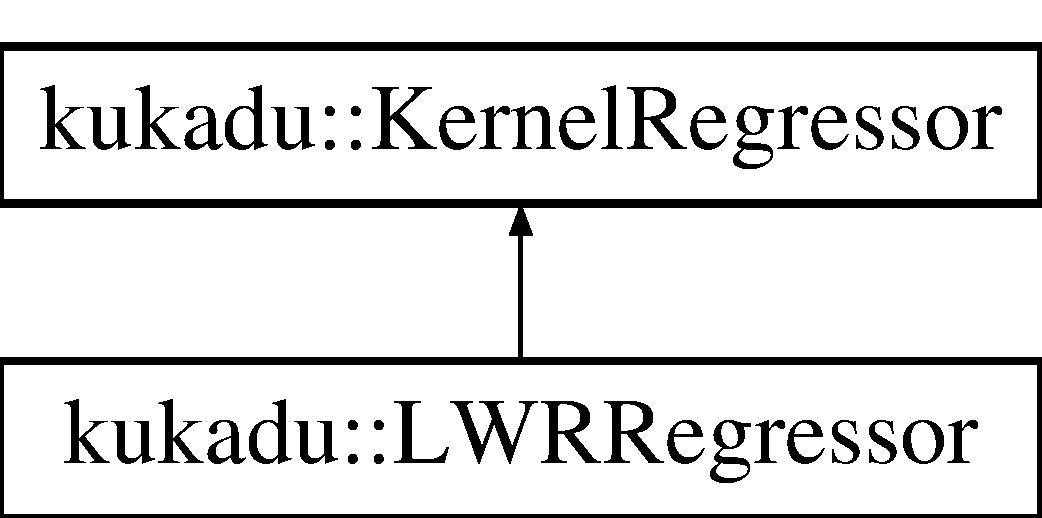
\includegraphics[height=2.000000cm]{classkukadu_1_1LWRRegressor}
\end{center}
\end{figure}
\subsection*{Public Member Functions}
\begin{DoxyCompactItemize}
\item 
\hyperlink{classkukadu_1_1LWRRegressor_a587e643f830a35a4ecdd21c1c8ac162a}{L\-W\-R\-Regressor} (std\-::vector$<$ arma\-::vec $>$ sample\-Xs, std\-::vector$<$ arma\-::vec $>$ sample\-Ts, \hyperlink{classkukadu_1_1GenericKernel}{Generic\-Kernel} $\ast$kernel, std\-::vector$<$ arma\-::mat $>$ design\-Matrices)
\begin{DoxyCompactList}\small\item\em constructor, setting all the sample data, the selected kernel and a vector of design matrices (one design matrix for each sample) \end{DoxyCompactList}\item 
arma\-::vec \hyperlink{classkukadu_1_1LWRRegressor_ae7d3e23243abefbfd47677967b60918b}{fit\-At\-Position} (arma\-::vec pos)
\begin{DoxyCompactList}\small\item\em performs the kernel method for predicting the functin value at a given position \end{DoxyCompactList}\end{DoxyCompactItemize}


\subsection{Detailed Description}
Implements the locally weighted regression method. 

This class inherits from the \hyperlink{classkukadu_1_1KernelRegressor}{Kernel\-Regressor} and implements locally weighted regression. It reuses the design matrices computed by the \hyperlink{classkukadu_1_1GeneralFitter}{General\-Fitter} class. 

\subsection{Constructor \& Destructor Documentation}
\hypertarget{classkukadu_1_1LWRRegressor_a587e643f830a35a4ecdd21c1c8ac162a}{\index{kukadu\-::\-L\-W\-R\-Regressor@{kukadu\-::\-L\-W\-R\-Regressor}!L\-W\-R\-Regressor@{L\-W\-R\-Regressor}}
\index{L\-W\-R\-Regressor@{L\-W\-R\-Regressor}!kukadu::LWRRegressor@{kukadu\-::\-L\-W\-R\-Regressor}}
\subsubsection[{L\-W\-R\-Regressor}]{\setlength{\rightskip}{0pt plus 5cm}kukadu\-::\-L\-W\-R\-Regressor\-::\-L\-W\-R\-Regressor (
\begin{DoxyParamCaption}
\item[{std\-::vector$<$ arma\-::vec $>$}]{sample\-Xs, }
\item[{std\-::vector$<$ arma\-::vec $>$}]{sample\-Ts, }
\item[{{\bf Generic\-Kernel} $\ast$}]{kernel, }
\item[{std\-::vector$<$ arma\-::mat $>$}]{design\-Matrices}
\end{DoxyParamCaption}
)}}\label{classkukadu_1_1LWRRegressor_a587e643f830a35a4ecdd21c1c8ac162a}


constructor, setting all the sample data, the selected kernel and a vector of design matrices (one design matrix for each sample) 


\begin{DoxyParams}{Parameters}
{\em sample\-Xs} & vector of samples (x-\/axis) \\
\hline
{\em sample\-Ts} & vector of samples (y-\/axis) \\
\hline
{\em kernel} & the selected kernel implementation \\
\hline
{\em design\-Matrices} & vector of design matrices \\
\hline
\end{DoxyParams}


\subsection{Member Function Documentation}
\hypertarget{classkukadu_1_1LWRRegressor_ae7d3e23243abefbfd47677967b60918b}{\index{kukadu\-::\-L\-W\-R\-Regressor@{kukadu\-::\-L\-W\-R\-Regressor}!fit\-At\-Position@{fit\-At\-Position}}
\index{fit\-At\-Position@{fit\-At\-Position}!kukadu::LWRRegressor@{kukadu\-::\-L\-W\-R\-Regressor}}
\subsubsection[{fit\-At\-Position}]{\setlength{\rightskip}{0pt plus 5cm}vec kukadu\-::\-L\-W\-R\-Regressor\-::fit\-At\-Position (
\begin{DoxyParamCaption}
\item[{arma\-::vec}]{pos}
\end{DoxyParamCaption}
)\hspace{0.3cm}{\ttfamily [virtual]}}}\label{classkukadu_1_1LWRRegressor_ae7d3e23243abefbfd47677967b60918b}


performs the kernel method for predicting the functin value at a given position 


\begin{DoxyParams}{Parameters}
{\em pos} & vector defining the required position \\
\hline
\end{DoxyParams}


Implements \hyperlink{classkukadu_1_1KernelRegressor_afd1489310e11cff4bd88390ba76c38e1}{kukadu\-::\-Kernel\-Regressor}.



The documentation for this class was generated from the following files\-:\begin{DoxyCompactItemize}
\item 
/home/c7031109/iis\-\_\-robot\-\_\-sw/iis\-\_\-catkin\-\_\-ws/src/kukadu/include/kukadu/learning/regression/lwrregressor.\-hpp\item 
/home/c7031109/iis\-\_\-robot\-\_\-sw/iis\-\_\-catkin\-\_\-ws/src/kukadu/src/learning/lwrregressor.\-cpp\end{DoxyCompactItemize}

\hypertarget{classkukadu_1_1Mahalanobis}{\section{kukadu\-:\-:Mahalanobis Class Reference}
\label{classkukadu_1_1Mahalanobis}\index{kukadu\-::\-Mahalanobis@{kukadu\-::\-Mahalanobis}}
}
\subsection*{Public Member Functions}
\begin{DoxyCompactItemize}
\item 
\hypertarget{classkukadu_1_1Mahalanobis_a15f47cbf891794a56efda7d108fbd7ec}{{\bfseries Mahalanobis} (int dim)}\label{classkukadu_1_1Mahalanobis_a15f47cbf891794a56efda7d108fbd7ec}

\item 
\hypertarget{classkukadu_1_1Mahalanobis_a88c4934e79958652ed59fe146c387980}{{\bfseries Mahalanobis} (arma\-::mat M)}\label{classkukadu_1_1Mahalanobis_a88c4934e79958652ed59fe146c387980}

\item 
\hypertarget{classkukadu_1_1Mahalanobis_a1a6e0cb4e5ae21e69b719bf4352ebaf7}{{\bfseries Mahalanobis} (const \hyperlink{classkukadu_1_1Mahalanobis}{Mahalanobis} \&maha)}\label{classkukadu_1_1Mahalanobis_a1a6e0cb4e5ae21e69b719bf4352ebaf7}

\item 
\hypertarget{classkukadu_1_1Mahalanobis_a4908373882185f929f90910496d0be46}{double {\bfseries compute\-Squared\-Distance} (arma\-::vec vec1, arma\-::vec vec2)}\label{classkukadu_1_1Mahalanobis_a4908373882185f929f90910496d0be46}

\item 
\hypertarget{classkukadu_1_1Mahalanobis_ab5215c5132db0326d6cdcebca8d4473f}{arma\-::vec {\bfseries get\-Coefficients} ()}\label{classkukadu_1_1Mahalanobis_ab5215c5132db0326d6cdcebca8d4473f}

\item 
\hypertarget{classkukadu_1_1Mahalanobis_afc94f534bc63e0ff416d69a51b4b9c6f}{void {\bfseries set\-M} (arma\-::mat M)}\label{classkukadu_1_1Mahalanobis_afc94f534bc63e0ff416d69a51b4b9c6f}

\item 
\hypertarget{classkukadu_1_1Mahalanobis_a6a6db9d96a3b59c9129434a71223f3e1}{arma\-::mat {\bfseries get\-M} () const }\label{classkukadu_1_1Mahalanobis_a6a6db9d96a3b59c9129434a71223f3e1}

\item 
\hypertarget{classkukadu_1_1Mahalanobis_a65b487f0373df5c13dee4826e379fdff}{arma\-::mat {\bfseries get\-Decomposition} ()}\label{classkukadu_1_1Mahalanobis_a65b487f0373df5c13dee4826e379fdff}

\end{DoxyCompactItemize}


The documentation for this class was generated from the following files\-:\begin{DoxyCompactItemize}
\item 
/home/c7031109/iis\-\_\-robot\-\_\-sw/iis\-\_\-catkin\-\_\-ws/src/kukadu/include/kukadu/learning/metric\-\_\-learning/mahalanobis.\-hpp\item 
/home/c7031109/iis\-\_\-robot\-\_\-sw/iis\-\_\-catkin\-\_\-ws/src/kukadu/src/learning/metric\-\_\-learning/mahalanobis.\-cpp\end{DoxyCompactItemize}

\hypertarget{classkukadu_1_1MahalanobisLearner}{\section{kukadu\-:\-:Mahalanobis\-Learner Class Reference}
\label{classkukadu_1_1MahalanobisLearner}\index{kukadu\-::\-Mahalanobis\-Learner@{kukadu\-::\-Mahalanobis\-Learner}}
}
Inheritance diagram for kukadu\-:\-:Mahalanobis\-Learner\-:\begin{figure}[H]
\begin{center}
\leavevmode
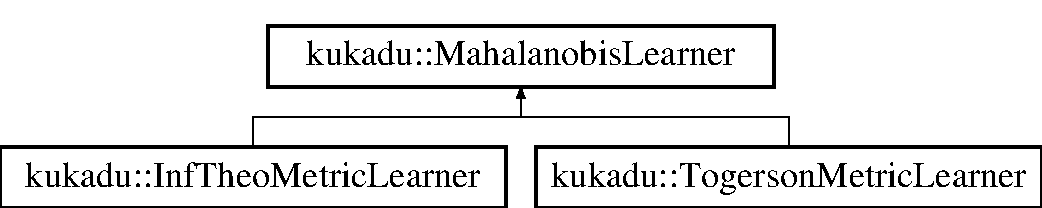
\includegraphics[height=2.000000cm]{classkukadu_1_1MahalanobisLearner}
\end{center}
\end{figure}
\subsection*{Public Member Functions}
\begin{DoxyCompactItemize}
\item 
\hypertarget{classkukadu_1_1MahalanobisLearner_a9f9d3dffef0fad99e19e54e4ce99e9d2}{{\bfseries Mahalanobis\-Learner} (std\-::vector$<$ arma\-::vec $>$ x1s, std\-::vector$<$ arma\-::vec $>$ x2s, std\-::vector$<$ double $>$ distances)}\label{classkukadu_1_1MahalanobisLearner_a9f9d3dffef0fad99e19e54e4ce99e9d2}

\item 
\hypertarget{classkukadu_1_1MahalanobisLearner_a4f3b38ac5088b27d34a2bc8200aa8dce}{void {\bfseries add\-Sample} (arma\-::vec x1, arma\-::vec x2, double distance)}\label{classkukadu_1_1MahalanobisLearner_a4f3b38ac5088b27d34a2bc8200aa8dce}

\item 
\hypertarget{classkukadu_1_1MahalanobisLearner_af57c5d3f3876acc201e923a55db342ca}{int {\bfseries get\-Sample\-Count} ()}\label{classkukadu_1_1MahalanobisLearner_af57c5d3f3876acc201e923a55db342ca}

\item 
\hypertarget{classkukadu_1_1MahalanobisLearner_a24d0f7f9e43d297454aa316f80019e15}{int {\bfseries get\-Vector\-Dim} ()}\label{classkukadu_1_1MahalanobisLearner_a24d0f7f9e43d297454aa316f80019e15}

\item 
\hypertarget{classkukadu_1_1MahalanobisLearner_aeb08af8a9bbf6d482a7bbdb1c34e933b}{double {\bfseries get\-Sample\-Distance} (int idx)}\label{classkukadu_1_1MahalanobisLearner_aeb08af8a9bbf6d482a7bbdb1c34e933b}

\item 
\hypertarget{classkukadu_1_1MahalanobisLearner_ac552c824300edabfc56f097f8adfea4a}{arma\-::vec {\bfseries get\-X1} (int idx)}\label{classkukadu_1_1MahalanobisLearner_ac552c824300edabfc56f097f8adfea4a}

\item 
\hypertarget{classkukadu_1_1MahalanobisLearner_a43027e86750acf224b07edbe63514a2b}{arma\-::vec {\bfseries get\-X2} (int idx)}\label{classkukadu_1_1MahalanobisLearner_a43027e86750acf224b07edbe63514a2b}

\item 
\hypertarget{classkukadu_1_1MahalanobisLearner_a66f0a4fbe1aef2a2eb8434552fe6a556}{\hyperlink{classkukadu_1_1Mahalanobis}{Mahalanobis} {\bfseries get\-Metric} ()}\label{classkukadu_1_1MahalanobisLearner_a66f0a4fbe1aef2a2eb8434552fe6a556}

\item 
\hypertarget{classkukadu_1_1MahalanobisLearner_a05b61576c302b5484bc1a482968c01a0}{virtual \hyperlink{classkukadu_1_1Mahalanobis}{Mahalanobis} {\bfseries learn\-Metric} ()=0}\label{classkukadu_1_1MahalanobisLearner_a05b61576c302b5484bc1a482968c01a0}

\end{DoxyCompactItemize}
\subsection*{Protected Attributes}
\begin{DoxyCompactItemize}
\item 
\hypertarget{classkukadu_1_1MahalanobisLearner_a3ea033162dbf7ac4abec5411551893ca}{std\-::vector$<$ arma\-::vec $>$ {\bfseries x1s}}\label{classkukadu_1_1MahalanobisLearner_a3ea033162dbf7ac4abec5411551893ca}

\item 
\hypertarget{classkukadu_1_1MahalanobisLearner_ae0e587ea27bf3d609707a4eb6f919277}{std\-::vector$<$ arma\-::vec $>$ {\bfseries x2s}}\label{classkukadu_1_1MahalanobisLearner_ae0e587ea27bf3d609707a4eb6f919277}

\item 
\hypertarget{classkukadu_1_1MahalanobisLearner_af587d7f1d1679175071497d4c37ceef9}{std\-::vector$<$ double $>$ {\bfseries distances}}\label{classkukadu_1_1MahalanobisLearner_af587d7f1d1679175071497d4c37ceef9}

\end{DoxyCompactItemize}


The documentation for this class was generated from the following files\-:\begin{DoxyCompactItemize}
\item 
/home/c7031109/iis\-\_\-robot\-\_\-sw/iis\-\_\-catkin\-\_\-ws/src/kukadu/include/kukadu/learning/metric\-\_\-learning/mahalanobicslearner.\-hpp\item 
/home/c7031109/iis\-\_\-robot\-\_\-sw/iis\-\_\-catkin\-\_\-ws/src/kukadu/src/learning/metric\-\_\-learning/mahalanobicslearner.\-cpp\end{DoxyCompactItemize}

\hypertarget{classkukadu_1_1ManualReward}{\section{kukadu\-:\-:Manual\-Reward Class Reference}
\label{classkukadu_1_1ManualReward}\index{kukadu\-::\-Manual\-Reward@{kukadu\-::\-Manual\-Reward}}
}
Inheritance diagram for kukadu\-:\-:Manual\-Reward\-:\begin{figure}[H]
\begin{center}
\leavevmode
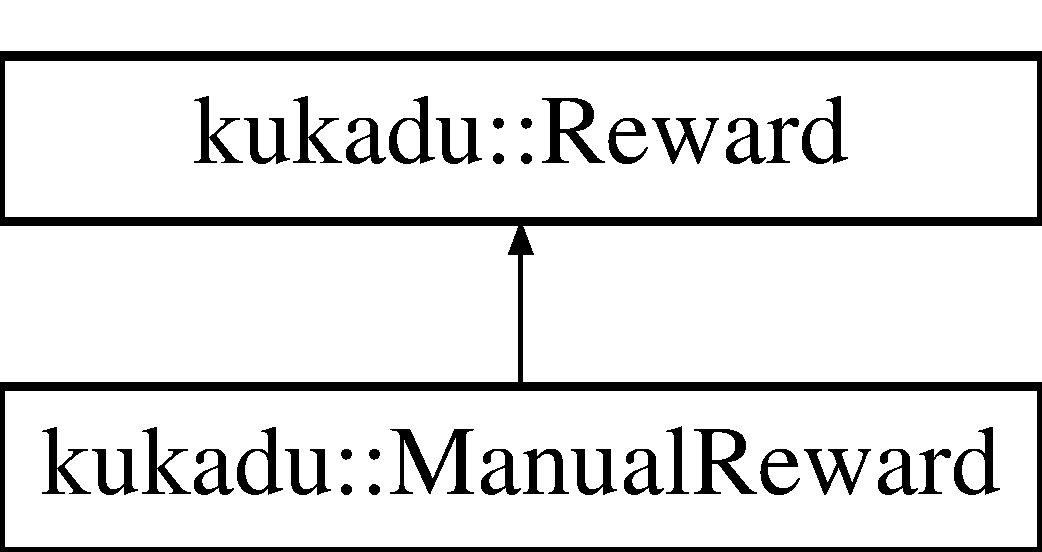
\includegraphics[height=2.000000cm]{classkukadu_1_1ManualReward}
\end{center}
\end{figure}
\subsection*{Public Member Functions}
\begin{DoxyCompactItemize}
\item 
\hypertarget{classkukadu_1_1ManualReward_a318822b732a0011ff4ff7cc8ff3d1a05}{{\bfseries Manual\-Reward} (K\-U\-K\-A\-D\-U\-\_\-\-S\-H\-A\-R\-E\-D\-\_\-\-P\-T\-R$<$ kukadu\-\_\-mersenne\-\_\-twister $>$ generator, int number\-Of\-Actions, int number\-Of\-Percepts, bool collect\-Prev\-Rewards, double std\-Reward)}\label{classkukadu_1_1ManualReward_a318822b732a0011ff4ff7cc8ff3d1a05}

\item 
\hypertarget{classkukadu_1_1ManualReward_a5822e7d8bef85ce182c0c8c82651cc33}{void {\bfseries set\-Next\-Percept\-Id} (int next\-Id)}\label{classkukadu_1_1ManualReward_a5822e7d8bef85ce182c0c8c82651cc33}

\item 
\hypertarget{classkukadu_1_1ManualReward_a0c22cd7ef3f972b6294ace8847283403}{int {\bfseries get\-Dimensionality} ()}\label{classkukadu_1_1ManualReward_a0c22cd7ef3f972b6294ace8847283403}

\item 
\hypertarget{classkukadu_1_1ManualReward_a0fc7e055ddabdf964dc073b795a6b701}{K\-U\-K\-A\-D\-U\-\_\-\-S\-H\-A\-R\-E\-D\-\_\-\-P\-T\-R$<$ \hyperlink{classkukadu_1_1PerceptClip}{Percept\-Clip} $>$ {\bfseries generate\-Next\-Percept\-Clip} (int immunity)}\label{classkukadu_1_1ManualReward_a0fc7e055ddabdf964dc073b795a6b701}

\item 
\hypertarget{classkukadu_1_1ManualReward_ab265fb63722a405fa1b5cfaa9d96b47f}{K\-U\-K\-A\-D\-U\-\_\-\-S\-H\-A\-R\-E\-D\-\_\-\-P\-T\-R$<$ std\-::vector\\*
$<$ K\-U\-K\-A\-D\-U\-\_\-\-S\-H\-A\-R\-E\-D\-\_\-\-P\-T\-R\\*
$<$ \hyperlink{classkukadu_1_1ActionClip}{Action\-Clip} $>$ $>$ $>$ {\bfseries generate\-Action\-Clips} ()}\label{classkukadu_1_1ManualReward_ab265fb63722a405fa1b5cfaa9d96b47f}

\item 
\hypertarget{classkukadu_1_1ManualReward_a6bc98a96fc54aaad311d35c7b1043d65}{K\-U\-K\-A\-D\-U\-\_\-\-S\-H\-A\-R\-E\-D\-\_\-\-P\-T\-R$<$ std\-::vector\\*
$<$ K\-U\-K\-A\-D\-U\-\_\-\-S\-H\-A\-R\-E\-D\-\_\-\-P\-T\-R\\*
$<$ \hyperlink{classkukadu_1_1PerceptClip}{Percept\-Clip} $>$ $>$ $>$ {\bfseries generate\-Percept\-Clips} ()}\label{classkukadu_1_1ManualReward_a6bc98a96fc54aaad311d35c7b1043d65}

\end{DoxyCompactItemize}
\subsection*{Protected Member Functions}
\begin{DoxyCompactItemize}
\item 
\hypertarget{classkukadu_1_1ManualReward_accd1c514e0c2e4f64c80dc8dc0dd3a43}{double {\bfseries compute\-Reward\-Internal} (K\-U\-K\-A\-D\-U\-\_\-\-S\-H\-A\-R\-E\-D\-\_\-\-P\-T\-R$<$ \hyperlink{classkukadu_1_1PerceptClip}{Percept\-Clip} $>$ provided\-Percept, K\-U\-K\-A\-D\-U\-\_\-\-S\-H\-A\-R\-E\-D\-\_\-\-P\-T\-R$<$ \hyperlink{classkukadu_1_1ActionClip}{Action\-Clip} $>$ taken\-Action)}\label{classkukadu_1_1ManualReward_accd1c514e0c2e4f64c80dc8dc0dd3a43}

\end{DoxyCompactItemize}
\subsection*{Additional Inherited Members}


The documentation for this class was generated from the following files\-:\begin{DoxyCompactItemize}
\item 
/home/c7031109/iis\-\_\-robot\-\_\-sw/iis\-\_\-catkin\-\_\-ws/src/kukadu/include/kukadu/learning/projective\-\_\-simulation/application/manualreward.\-hpp\item 
/home/c7031109/iis\-\_\-robot\-\_\-sw/iis\-\_\-catkin\-\_\-ws/src/kukadu/src/learning/projective\-\_\-simulation/application/manualreward.\-cpp\end{DoxyCompactItemize}

\hypertarget{structmes__result}{\section{mes\-\_\-result \-Struct \-Reference}
\label{structmes__result}\index{mes\-\_\-result@{mes\-\_\-result}}
}


{\ttfamily \#include $<$types.\-h$>$}

\subsection*{\-Public \-Attributes}
\begin{DoxyCompactItemize}
\item 
float $\ast$ \hyperlink{structmes__result_a332fdbaad9f2ba4bda329195c3ce8eda}{joints}
\end{DoxyCompactItemize}


\subsection{\-Member \-Data \-Documentation}
\hypertarget{structmes__result_a332fdbaad9f2ba4bda329195c3ce8eda}{\index{mes\-\_\-result@{mes\-\_\-result}!joints@{joints}}
\index{joints@{joints}!mes_result@{mes\-\_\-result}}
\subsubsection[{joints}]{\setlength{\rightskip}{0pt plus 5cm}float$\ast$ {\bf mes\-\_\-result\-::joints}}}\label{structmes__result_a332fdbaad9f2ba4bda329195c3ce8eda}


\-The documentation for this struct was generated from the following file\-:\begin{DoxyCompactItemize}
\item 
/home/shangl/data/data\-\_\-synched/studium/informatik/master/master\-\_\-thesis/kukadu\-\_\-framework/thesis/src/utils/\hyperlink{types_8h}{types.\-h}\end{DoxyCompactItemize}

\hypertarget{classkukadu_1_1MoveItConstraint}{\section{kukadu\-:\-:Move\-It\-Constraint Class Reference}
\label{classkukadu_1_1MoveItConstraint}\index{kukadu\-::\-Move\-It\-Constraint@{kukadu\-::\-Move\-It\-Constraint}}
}
Inheritance diagram for kukadu\-:\-:Move\-It\-Constraint\-:\begin{figure}[H]
\begin{center}
\leavevmode
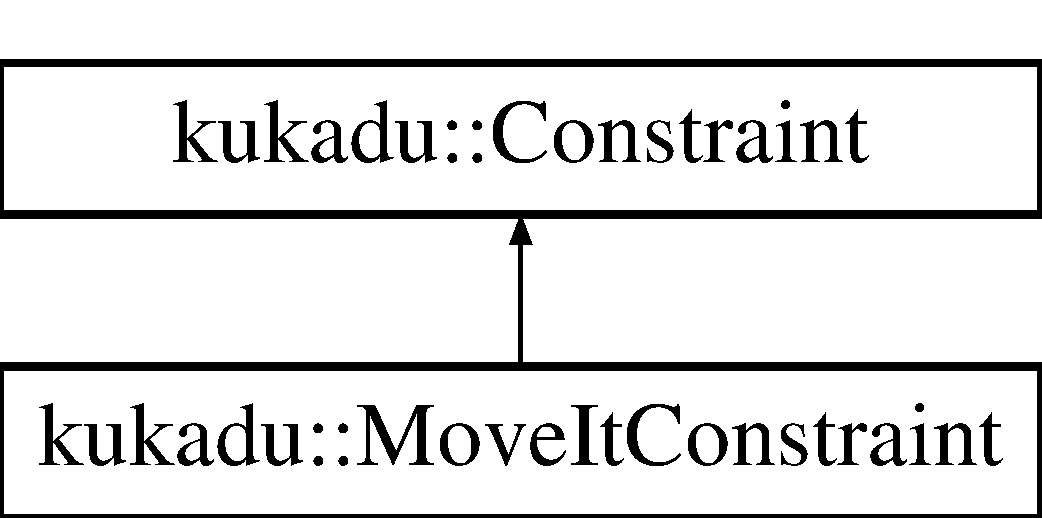
\includegraphics[height=2.000000cm]{classkukadu_1_1MoveItConstraint}
\end{center}
\end{figure}
\subsection*{Public Member Functions}
\begin{DoxyCompactItemize}
\item 
\hypertarget{classkukadu_1_1MoveItConstraint_a8c238ba81d91e292334a1f7fc58366d2}{{\bfseries Move\-It\-Constraint} (robot\-\_\-model\-::\-Robot\-Model\-Ptr, planning\-\_\-scene\-::\-Planning\-Scene\-Ptr planning\-Scene, moveit\-::core\-::\-Joint\-Model\-Group $\ast$model\-Group)}\label{classkukadu_1_1MoveItConstraint_a8c238ba81d91e292334a1f7fc58366d2}

\item 
\hypertarget{classkukadu_1_1MoveItConstraint_a9454a3a164f71145b89d8df88dcbab2f}{virtual std\-::string {\bfseries get\-Constraint\-Name} ()}\label{classkukadu_1_1MoveItConstraint_a9454a3a164f71145b89d8df88dcbab2f}

\item 
\hypertarget{classkukadu_1_1MoveItConstraint_a32ad1c00688ae65a244708cac486bb03}{virtual bool {\bfseries state\-Ok} (arma\-::vec joint, geometry\-\_\-msgs\-::\-Pose cart\-Pose)}\label{classkukadu_1_1MoveItConstraint_a32ad1c00688ae65a244708cac486bb03}

\end{DoxyCompactItemize}


The documentation for this class was generated from the following files\-:\begin{DoxyCompactItemize}
\item 
/home/c7031109/iis\-\_\-robot\-\_\-sw/iis\-\_\-catkin\-\_\-ws/src/kukadu/include/kukadu/kinematics/constraints/constraints.\-hpp\item 
/home/c7031109/iis\-\_\-robot\-\_\-sw/iis\-\_\-catkin\-\_\-ws/src/kukadu/src/kinematics/constraints/constraints.\-cpp\end{DoxyCompactItemize}

\hypertarget{classkukadu_1_1MoveItKinematics}{\section{kukadu\-:\-:Move\-It\-Kinematics Class Reference}
\label{classkukadu_1_1MoveItKinematics}\index{kukadu\-::\-Move\-It\-Kinematics@{kukadu\-::\-Move\-It\-Kinematics}}
}
Inheritance diagram for kukadu\-:\-:Move\-It\-Kinematics\-:\begin{figure}[H]
\begin{center}
\leavevmode
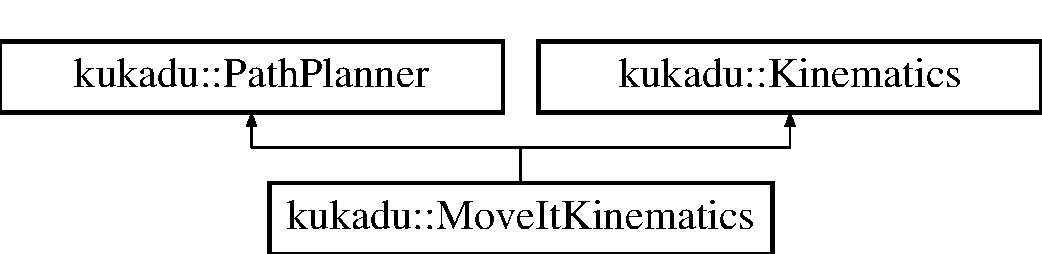
\includegraphics[height=2.000000cm]{classkukadu_1_1MoveItKinematics}
\end{center}
\end{figure}
\subsection*{Public Member Functions}
\begin{DoxyCompactItemize}
\item 
\hypertarget{classkukadu_1_1MoveItKinematics_a2014973f734e343eab24ee034b4136ae}{{\bfseries Move\-It\-Kinematics} (K\-U\-K\-A\-D\-U\-\_\-\-S\-H\-A\-R\-E\-D\-\_\-\-P\-T\-R$<$ \hyperlink{classkukadu_1_1ControlQueue}{Control\-Queue} $>$ queue, ros\-::\-Node\-Handle node, std\-::string move\-Group\-Name, std\-::vector$<$ std\-::string $>$ joint\-Names, std\-::string tip\-Link)}\label{classkukadu_1_1MoveItKinematics_a2014973f734e343eab24ee034b4136ae}

\item 
\hypertarget{classkukadu_1_1MoveItKinematics_a5b4c08edeb86780f498525d03669faf5}{{\bfseries Move\-It\-Kinematics} (K\-U\-K\-A\-D\-U\-\_\-\-S\-H\-A\-R\-E\-D\-\_\-\-P\-T\-R$<$ \hyperlink{classkukadu_1_1ControlQueue}{Control\-Queue} $>$ queue, ros\-::\-Node\-Handle node, std\-::string move\-Group\-Name, std\-::vector$<$ std\-::string $>$ joint\-Names, std\-::string tip\-Link, bool avoid\-Collisions, int max\-Attempts, double time\-Out)}\label{classkukadu_1_1MoveItKinematics_a5b4c08edeb86780f498525d03669faf5}

\item 
\hypertarget{classkukadu_1_1MoveItKinematics_a5e0335477c0b1880b1c1cd8ce281933a}{virtual geometry\-\_\-msgs\-::\-Pose {\bfseries compute\-Fk} (std\-::vector$<$ double $>$ joint\-State)}\label{classkukadu_1_1MoveItKinematics_a5e0335477c0b1880b1c1cd8ce281933a}

\item 
\hypertarget{classkukadu_1_1MoveItKinematics_ac79665569fe1c5dde2623c2de0d450f0}{virtual std\-::vector$<$ arma\-::vec $>$ {\bfseries compute\-Ik} (std\-::vector$<$ double $>$ current\-Joint\-State, const geometry\-\_\-msgs\-::\-Pose \&goal)}\label{classkukadu_1_1MoveItKinematics_ac79665569fe1c5dde2623c2de0d450f0}

\item 
\hypertarget{classkukadu_1_1MoveItKinematics_a8e4bd89a6483eff718671d2877297da8}{virtual std\-::vector$<$ arma\-::vec $>$ {\bfseries plan\-Joint\-Trajectory} (std\-::vector$<$ arma\-::vec $>$ intermediate\-Joints)}\label{classkukadu_1_1MoveItKinematics_a8e4bd89a6483eff718671d2877297da8}

\item 
\hypertarget{classkukadu_1_1MoveItKinematics_a1a51e4de20c5b79eccf09ad547de6914}{virtual std\-::vector$<$ arma\-::vec $>$ {\bfseries plan\-Cartesian\-Trajectory} (std\-::vector$<$ geometry\-\_\-msgs\-::\-Pose $>$ intermediate\-Poses, bool smooth\-Cartesians=false, bool use\-Current\-Robot\-State=true)}\label{classkukadu_1_1MoveItKinematics_a1a51e4de20c5b79eccf09ad547de6914}

\item 
\hypertarget{classkukadu_1_1MoveItKinematics_a51f3a5d4e74240413173c7e9a7c1b454}{virtual std\-::vector$<$ arma\-::vec $>$ {\bfseries plan\-Cartesian\-Trajectory} (arma\-::vec start\-Joints, std\-::vector$<$ geometry\-\_\-msgs\-::\-Pose $>$ intermediate\-Poses, bool smooth\-Cartesians=false, bool use\-Current\-Robot\-State=true)}\label{classkukadu_1_1MoveItKinematics_a51f3a5d4e74240413173c7e9a7c1b454}

\item 
\hypertarget{classkukadu_1_1MoveItKinematics_ae51321ad291b1028a08ed778e8648a69}{bool {\bfseries is\-Colliding} (arma\-::vec joint\-State, geometry\-\_\-msgs\-::\-Pose pose)}\label{classkukadu_1_1MoveItKinematics_ae51321ad291b1028a08ed778e8648a69}

\item 
\hypertarget{classkukadu_1_1MoveItKinematics_a529444d890549bcf9b6c53f94a340040}{K\-U\-K\-A\-D\-U\-\_\-\-S\-H\-A\-R\-E\-D\-\_\-\-P\-T\-R$<$ \hyperlink{classkukadu_1_1Constraint}{Constraint} $>$ {\bfseries get\-Model\-Constraint} ()}\label{classkukadu_1_1MoveItKinematics_a529444d890549bcf9b6c53f94a340040}

\end{DoxyCompactItemize}
\subsection*{Static Public Attributes}
\begin{DoxyCompactItemize}
\item 
\hypertarget{classkukadu_1_1MoveItKinematics_ae539766efac62822c841cf211c666ce1}{static const int {\bfseries S\-T\-D\-\_\-\-M\-A\-X\-\_\-\-A\-T\-T\-E\-M\-P\-T\-S} = 5}\label{classkukadu_1_1MoveItKinematics_ae539766efac62822c841cf211c666ce1}

\item 
\hypertarget{classkukadu_1_1MoveItKinematics_a5172477ff4cdf5f48bb8a2b1a2e453e8}{static const double {\bfseries S\-T\-D\-\_\-\-T\-I\-M\-E\-O\-U\-T} = 0.\-1}\label{classkukadu_1_1MoveItKinematics_a5172477ff4cdf5f48bb8a2b1a2e453e8}

\item 
\hypertarget{classkukadu_1_1MoveItKinematics_af3bfbf694219dc9784ffd78093d32913}{static const bool {\bfseries S\-T\-D\-\_\-\-A\-V\-O\-I\-D\-\_\-\-C\-O\-L\-L\-I\-S\-I\-O\-N\-S} = true}\label{classkukadu_1_1MoveItKinematics_af3bfbf694219dc9784ffd78093d32913}

\end{DoxyCompactItemize}


The documentation for this class was generated from the following files\-:\begin{DoxyCompactItemize}
\item 
/home/c7031109/iis\-\_\-robot\-\_\-sw/iis\-\_\-catkin\-\_\-ws/src/kukadu/include/kukadu/kinematics/moveitkinematics.\-hpp\item 
/home/c7031109/iis\-\_\-robot\-\_\-sw/iis\-\_\-catkin\-\_\-ws/src/kukadu/src/kinematics/moveitkinematics.\-cpp\end{DoxyCompactItemize}

\hypertarget{classkukadu_1_1NeverendingColorReward}{\section{kukadu\-:\-:Neverending\-Color\-Reward Class Reference}
\label{classkukadu_1_1NeverendingColorReward}\index{kukadu\-::\-Neverending\-Color\-Reward@{kukadu\-::\-Neverending\-Color\-Reward}}
}
Inheritance diagram for kukadu\-:\-:Neverending\-Color\-Reward\-:\begin{figure}[H]
\begin{center}
\leavevmode
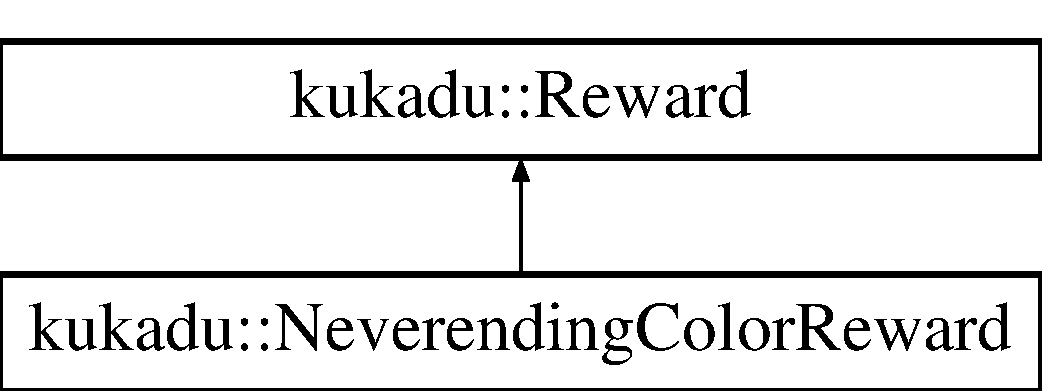
\includegraphics[height=2.000000cm]{classkukadu_1_1NeverendingColorReward}
\end{center}
\end{figure}
\subsection*{Public Member Functions}
\begin{DoxyCompactItemize}
\item 
\hypertarget{classkukadu_1_1NeverendingColorReward_adb679e39345857002e31754eefb85c0f}{{\bfseries Neverending\-Color\-Reward} (K\-U\-K\-A\-D\-U\-\_\-\-S\-H\-A\-R\-E\-D\-\_\-\-P\-T\-R$<$ kukadu\-\_\-mersenne\-\_\-twister $>$ generator, int number\-Of\-Actions, int number\-Of\-Categories, bool collect\-Prev\-Rewards)}\label{classkukadu_1_1NeverendingColorReward_adb679e39345857002e31754eefb85c0f}

\item 
\hypertarget{classkukadu_1_1NeverendingColorReward_a9a58636526eb87b70c848e964a750036}{int {\bfseries get\-Dimensionality} ()}\label{classkukadu_1_1NeverendingColorReward_a9a58636526eb87b70c848e964a750036}

\item 
\hypertarget{classkukadu_1_1NeverendingColorReward_ac330bfc2bdb29562cd0d04b5b0c2b2e5}{K\-U\-K\-A\-D\-U\-\_\-\-S\-H\-A\-R\-E\-D\-\_\-\-P\-T\-R$<$ \hyperlink{classkukadu_1_1PerceptClip}{Percept\-Clip} $>$ {\bfseries generate\-Next\-Percept\-Clip} (int immunity)}\label{classkukadu_1_1NeverendingColorReward_ac330bfc2bdb29562cd0d04b5b0c2b2e5}

\item 
\hypertarget{classkukadu_1_1NeverendingColorReward_a0f346a8d39232fa23db7dedd7558c5c3}{K\-U\-K\-A\-D\-U\-\_\-\-S\-H\-A\-R\-E\-D\-\_\-\-P\-T\-R$<$ std\-::vector\\*
$<$ K\-U\-K\-A\-D\-U\-\_\-\-S\-H\-A\-R\-E\-D\-\_\-\-P\-T\-R\\*
$<$ \hyperlink{classkukadu_1_1ActionClip}{Action\-Clip} $>$ $>$ $>$ {\bfseries generate\-Action\-Clips} ()}\label{classkukadu_1_1NeverendingColorReward_a0f346a8d39232fa23db7dedd7558c5c3}

\item 
\hypertarget{classkukadu_1_1NeverendingColorReward_aed748e7ccf5eb06b37bad79f0b0fb2d8}{K\-U\-K\-A\-D\-U\-\_\-\-S\-H\-A\-R\-E\-D\-\_\-\-P\-T\-R$<$ std\-::vector\\*
$<$ K\-U\-K\-A\-D\-U\-\_\-\-S\-H\-A\-R\-E\-D\-\_\-\-P\-T\-R\\*
$<$ \hyperlink{classkukadu_1_1PerceptClip}{Percept\-Clip} $>$ $>$ $>$ {\bfseries generate\-Percept\-Clips} ()}\label{classkukadu_1_1NeverendingColorReward_aed748e7ccf5eb06b37bad79f0b0fb2d8}

\end{DoxyCompactItemize}
\subsection*{Protected Member Functions}
\begin{DoxyCompactItemize}
\item 
\hypertarget{classkukadu_1_1NeverendingColorReward_aebb2ab5ecbdf9d6c3c8a5ac4931c8891}{double {\bfseries compute\-Reward\-Internal} (K\-U\-K\-A\-D\-U\-\_\-\-S\-H\-A\-R\-E\-D\-\_\-\-P\-T\-R$<$ \hyperlink{classkukadu_1_1PerceptClip}{Percept\-Clip} $>$ provided\-Percept, K\-U\-K\-A\-D\-U\-\_\-\-S\-H\-A\-R\-E\-D\-\_\-\-P\-T\-R$<$ \hyperlink{classkukadu_1_1ActionClip}{Action\-Clip} $>$ taken\-Action)}\label{classkukadu_1_1NeverendingColorReward_aebb2ab5ecbdf9d6c3c8a5ac4931c8891}

\end{DoxyCompactItemize}
\subsection*{Additional Inherited Members}


The documentation for this class was generated from the following files\-:\begin{DoxyCompactItemize}
\item 
/home/c7031109/iis\-\_\-robot\-\_\-sw/iis\-\_\-catkin\-\_\-ws/src/kukadu/include/kukadu/learning/projective\-\_\-simulation/application/neverendingcolorreward.\-hpp\item 
/home/c7031109/iis\-\_\-robot\-\_\-sw/iis\-\_\-catkin\-\_\-ws/src/kukadu/src/learning/projective\-\_\-simulation/application/neverendingcolorreward.\-cpp\end{DoxyCompactItemize}

\hypertarget{classkukadu_1_1OpenBoxFilter}{\section{kukadu\-:\-:Open\-Box\-Filter Class Reference}
\label{classkukadu_1_1OpenBoxFilter}\index{kukadu\-::\-Open\-Box\-Filter@{kukadu\-::\-Open\-Box\-Filter}}
}
Inheritance diagram for kukadu\-:\-:Open\-Box\-Filter\-:\begin{figure}[H]
\begin{center}
\leavevmode
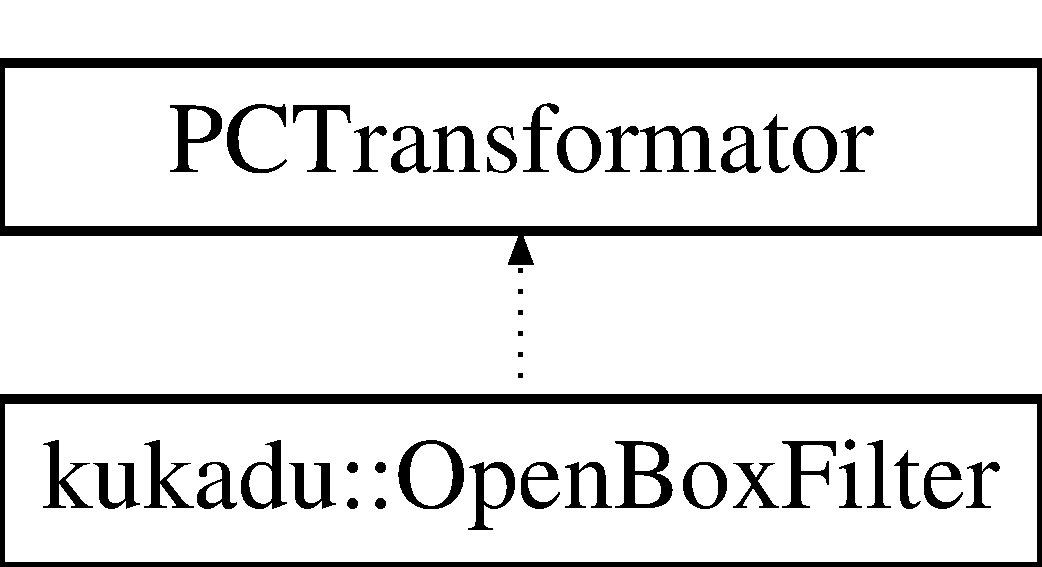
\includegraphics[height=2.000000cm]{classkukadu_1_1OpenBoxFilter}
\end{center}
\end{figure}
\subsection*{Public Member Functions}
\begin{DoxyCompactItemize}
\item 
\hypertarget{classkukadu_1_1OpenBoxFilter_a6e0307a97b104f1a14305502f6d16c18}{{\bfseries Open\-Box\-Filter} (arma\-::vec center, double x\-Offset, double y\-Offset)}\label{classkukadu_1_1OpenBoxFilter_a6e0307a97b104f1a14305502f6d16c18}

\item 
\hypertarget{classkukadu_1_1OpenBoxFilter_ab50cb129fdd531fa3033aa5de741a64c}{virtual pcl\-::\-Point\-Cloud\\*
$<$ pcl\-::\-Point\-X\-Y\-Z $>$\-::Ptr {\bfseries transform\-Pc} (pcl\-::\-Point\-Cloud$<$ pcl\-::\-Point\-X\-Y\-Z $>$\-::Ptr cloud)}\label{classkukadu_1_1OpenBoxFilter_ab50cb129fdd531fa3033aa5de741a64c}

\item 
\hypertarget{classkukadu_1_1OpenBoxFilter_a755530c495d178e1c4ec5a46df718aac}{void {\bfseries set\-Box} (arma\-::vec center, double x\-Offset, double y\-Offset)}\label{classkukadu_1_1OpenBoxFilter_a755530c495d178e1c4ec5a46df718aac}

\end{DoxyCompactItemize}


The documentation for this class was generated from the following files\-:\begin{DoxyCompactItemize}
\item 
/home/c7031109/iis\-\_\-robot\-\_\-sw/iis\-\_\-catkin\-\_\-ws/src/kukadu/include/kukadu/vision/openboxfilter.\-hpp\item 
/home/c7031109/iis\-\_\-robot\-\_\-sw/iis\-\_\-catkin\-\_\-ws/src/kukadu/src/vision/openboxfilter.\-cpp\end{DoxyCompactItemize}

\hypertarget{classkukadu_1_1PathPlanner}{\section{kukadu\-:\-:Path\-Planner Class Reference}
\label{classkukadu_1_1PathPlanner}\index{kukadu\-::\-Path\-Planner@{kukadu\-::\-Path\-Planner}}
}
Inheritance diagram for kukadu\-:\-:Path\-Planner\-:\begin{figure}[H]
\begin{center}
\leavevmode
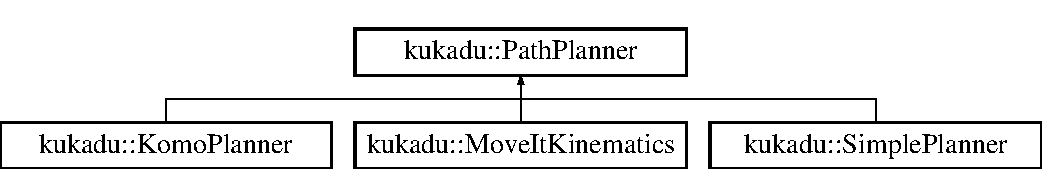
\includegraphics[height=2.000000cm]{classkukadu_1_1PathPlanner}
\end{center}
\end{figure}
\subsection*{Public Member Functions}
\begin{DoxyCompactItemize}
\item 
\hypertarget{classkukadu_1_1PathPlanner_a64bdab84aa8cf63b4c3a50f6ae0a9d7d}{void {\bfseries set\-Check\-Collisions} (bool collision)}\label{classkukadu_1_1PathPlanner_a64bdab84aa8cf63b4c3a50f6ae0a9d7d}

\item 
\hypertarget{classkukadu_1_1PathPlanner_ad807f61926f499a4b7dd277303156807}{bool {\bfseries get\-Check\-Collision} ()}\label{classkukadu_1_1PathPlanner_ad807f61926f499a4b7dd277303156807}

\item 
\hypertarget{classkukadu_1_1PathPlanner_ae10fe7292c94595d22a85b5f295af2bc}{virtual std\-::vector$<$ arma\-::vec $>$ {\bfseries smooth\-Joint\-Plan} (std\-::vector$<$ arma\-::vec $>$ joint\-Plan)}\label{classkukadu_1_1PathPlanner_ae10fe7292c94595d22a85b5f295af2bc}

\item 
\hypertarget{classkukadu_1_1PathPlanner_ab757c9af3406da8180bef68597b83542}{virtual std\-::vector$<$ arma\-::vec $>$ {\bfseries plan\-Joint\-Trajectory} (std\-::vector$<$ arma\-::vec $>$ intermediate\-Joints)=0}\label{classkukadu_1_1PathPlanner_ab757c9af3406da8180bef68597b83542}

\item 
\hypertarget{classkukadu_1_1PathPlanner_a959eb5545d65fdc108fdecad5d9d8542}{virtual std\-::vector$<$ arma\-::vec $>$ {\bfseries plan\-Cartesian\-Trajectory} (std\-::vector$<$ geometry\-\_\-msgs\-::\-Pose $>$ intermediate\-Poses, bool smooth\-Cartesians, bool use\-Current\-Robot\-State)=0}\label{classkukadu_1_1PathPlanner_a959eb5545d65fdc108fdecad5d9d8542}

\item 
\hypertarget{classkukadu_1_1PathPlanner_a7b3cf9ab52478e3d1775a17c9a6240e0}{virtual std\-::vector$<$ arma\-::vec $>$ {\bfseries plan\-Cartesian\-Trajectory} (arma\-::vec start\-Joints, std\-::vector$<$ geometry\-\_\-msgs\-::\-Pose $>$ intermediate\-Poses, bool smooth\-Cartesians=false, bool use\-Current\-Robot\-State=true)=0}\label{classkukadu_1_1PathPlanner_a7b3cf9ab52478e3d1775a17c9a6240e0}

\end{DoxyCompactItemize}
\subsection*{Static Public Attributes}
\begin{DoxyCompactItemize}
\item 
\hypertarget{classkukadu_1_1PathPlanner_a7baeae45bb2804b8142840ee96c7bcde}{static const int {\bfseries R\-E\-S\-U\-L\-T\-\_\-\-F\-A\-I\-L\-E\-D} = 0}\label{classkukadu_1_1PathPlanner_a7baeae45bb2804b8142840ee96c7bcde}

\item 
\hypertarget{classkukadu_1_1PathPlanner_a0e4f5875792d7d4c5e91f53d7d1d9f51}{static const int {\bfseries R\-E\-S\-U\-L\-T\-\_\-\-S\-U\-C\-C\-E\-S\-S} = 1}\label{classkukadu_1_1PathPlanner_a0e4f5875792d7d4c5e91f53d7d1d9f51}

\item 
\hypertarget{classkukadu_1_1PathPlanner_a41ed61ccf2715e4e838c12aaa7311e54}{static const int {\bfseries R\-E\-S\-U\-L\-T\-\_\-\-A\-P\-P\-R\-O\-X\-I\-M\-A\-T\-E} = 2}\label{classkukadu_1_1PathPlanner_a41ed61ccf2715e4e838c12aaa7311e54}

\end{DoxyCompactItemize}


The documentation for this class was generated from the following files\-:\begin{DoxyCompactItemize}
\item 
/home/c7031109/iis\-\_\-robot\-\_\-sw/iis\-\_\-catkin\-\_\-ws/src/kukadu/include/kukadu/kinematics/pathplanner.\-hpp\item 
/home/c7031109/iis\-\_\-robot\-\_\-sw/iis\-\_\-catkin\-\_\-ws/src/kukadu/src/kinematics/pathplanner.\-cpp\end{DoxyCompactItemize}

\hypertarget{classkukadu_1_1PCLTools}{\section{kukadu\-:\-:P\-C\-L\-Tools Class Reference}
\label{classkukadu_1_1PCLTools}\index{kukadu\-::\-P\-C\-L\-Tools@{kukadu\-::\-P\-C\-L\-Tools}}
}
\subsection*{Public Member Functions}
\begin{DoxyCompactItemize}
\item 
\hypertarget{classkukadu_1_1PCLTools_a14141dd30ae2c613b6547398bfe7b3d1}{void {\bfseries stop\-Visualization\-Window} ()}\label{classkukadu_1_1PCLTools_a14141dd30ae2c613b6547398bfe7b3d1}

\item 
\hypertarget{classkukadu_1_1PCLTools_a77ceff148e148532dfd6edef82aeba70}{void {\bfseries vis\-Draw\-Box} (std\-::string id, struct \hyperlink{structkukadu_1_1FitCube}{Fit\-Cube} dim)}\label{classkukadu_1_1PCLTools_a77ceff148e148532dfd6edef82aeba70}

\item 
\hypertarget{classkukadu_1_1PCLTools_a561208fa3e7334fb3541d39c18c2008c}{void {\bfseries vis\-Draw\-Plane\-With\-Normal} (std\-::string id, arma\-::vec r0, arma\-::vec n)}\label{classkukadu_1_1PCLTools_a561208fa3e7334fb3541d39c18c2008c}

\item 
\hypertarget{classkukadu_1_1PCLTools_a4964f97b079a8ec36b540bfb83d52853}{void {\bfseries visualize\-Point\-Cloud} (std\-::string id, pcl\-::\-Point\-Cloud$<$ pcl\-::\-Point\-X\-Y\-Z $>$\-::Ptr pc)}\label{classkukadu_1_1PCLTools_a4964f97b079a8ec36b540bfb83d52853}

\item 
\hypertarget{classkukadu_1_1PCLTools_a1c66a201e0907c90081d8b8940277563}{void {\bfseries update\-Visualized\-Point\-Cloud} (std\-::string id, pcl\-::\-Point\-Cloud$<$ pcl\-::\-Point\-X\-Y\-Z $>$\-::Ptr pc)}\label{classkukadu_1_1PCLTools_a1c66a201e0907c90081d8b8940277563}

\item 
\hypertarget{classkukadu_1_1PCLTools_a97b51443aea50669a88b3a0c4fd6b769}{K\-U\-K\-A\-D\-U\-\_\-\-S\-H\-A\-R\-E\-D\-\_\-\-P\-T\-R$<$ boost\-::thread $>$ {\bfseries initialize\-Visualization\-Window} ()}\label{classkukadu_1_1PCLTools_a97b51443aea50669a88b3a0c4fd6b769}

\item 
\hypertarget{classkukadu_1_1PCLTools_a99abc0b66655b8511f519c2f42c740be}{K\-U\-K\-A\-D\-U\-\_\-\-S\-H\-A\-R\-E\-D\-\_\-\-P\-T\-R\\*
$<$ pcl\-::visualization\-::\-P\-C\-L\-Visualizer $>$ {\bfseries get\-Visualizer} ()}\label{classkukadu_1_1PCLTools_a99abc0b66655b8511f519c2f42c740be}

\end{DoxyCompactItemize}
\subsection*{Static Public Member Functions}
\begin{DoxyCompactItemize}
\item 
\hypertarget{classkukadu_1_1PCLTools_aa5e8b8d3aa40a7370f2dcaa6ecdaa8ab}{static \hyperlink{structkukadu_1_1FitCube}{Fit\-Cube} {\bfseries fit\-Box} (pcl\-::\-Point\-Cloud$<$ pcl\-::\-Point\-X\-Y\-Z $>$\-::Ptr cloud)}\label{classkukadu_1_1PCLTools_aa5e8b8d3aa40a7370f2dcaa6ecdaa8ab}

\item 
\hypertarget{classkukadu_1_1PCLTools_a408c7df54bbd0de648cf0bdb1a4b8548}{static pcl\-::\-Point\-Cloud\\*
$<$ pcl\-::\-Point\-X\-Y\-Z $>$\-::Ptr {\bfseries segment\-Planar} (pcl\-::\-Point\-Cloud$<$ pcl\-::\-Point\-X\-Y\-Z $>$\-::Ptr cloud, bool negative)}\label{classkukadu_1_1PCLTools_a408c7df54bbd0de648cf0bdb1a4b8548}

\item 
\hypertarget{classkukadu_1_1PCLTools_a14c2a6fdf39b8b33f79c068d3a295999}{static pcl\-::\-Point\-Cloud\\*
$<$ pcl\-::\-Point\-X\-Y\-Z $>$\-::Ptr {\bfseries filter\-Cluster} (pcl\-::\-Point\-Cloud$<$ pcl\-::\-Point\-X\-Y\-Z $>$\-::Ptr cloud, bool negative)}\label{classkukadu_1_1PCLTools_a14c2a6fdf39b8b33f79c068d3a295999}

\end{DoxyCompactItemize}


The documentation for this class was generated from the following files\-:\begin{DoxyCompactItemize}
\item 
/home/c7031109/iis\-\_\-robot\-\_\-sw/iis\-\_\-catkin\-\_\-ws/src/kukadu/include/kukadu/vision/pcltools.\-hpp\item 
/home/c7031109/iis\-\_\-robot\-\_\-sw/iis\-\_\-catkin\-\_\-ws/src/kukadu/src/vision/pcltools.\-cpp\end{DoxyCompactItemize}

\hypertarget{classPCTransformator}{\section{P\-C\-Transformator Class Reference}
\label{classPCTransformator}\index{P\-C\-Transformator@{P\-C\-Transformator}}
}
Inheritance diagram for P\-C\-Transformator\-:\begin{figure}[H]
\begin{center}
\leavevmode
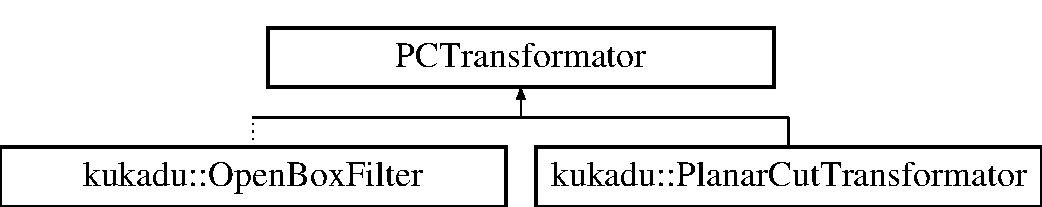
\includegraphics[height=2.000000cm]{classPCTransformator}
\end{center}
\end{figure}
\subsection*{Public Member Functions}
\begin{DoxyCompactItemize}
\item 
\hypertarget{classPCTransformator_a2fcc61667d7d668b49bc75240f419838}{virtual pcl\-::\-Point\-Cloud\\*
$<$ pcl\-::\-Point\-X\-Y\-Z $>$\-::Ptr {\bfseries transform\-Pc} (pcl\-::\-Point\-Cloud$<$ pcl\-::\-Point\-X\-Y\-Z $>$\-::Ptr pc)=0}\label{classPCTransformator_a2fcc61667d7d668b49bc75240f419838}

\end{DoxyCompactItemize}


The documentation for this class was generated from the following file\-:\begin{DoxyCompactItemize}
\item 
/home/c7031109/iis\-\_\-robot\-\_\-sw/iis\-\_\-catkin\-\_\-ws/src/kukadu/include/kukadu/vision/pcltransformator.\-hpp\end{DoxyCompactItemize}

\hypertarget{classkukadu_1_1PerceptClip}{\section{kukadu\-:\-:Percept\-Clip Class Reference}
\label{classkukadu_1_1PerceptClip}\index{kukadu\-::\-Percept\-Clip@{kukadu\-::\-Percept\-Clip}}
}
Inheritance diagram for kukadu\-:\-:Percept\-Clip\-:\begin{figure}[H]
\begin{center}
\leavevmode
\includegraphics[height=3.000000cm]{classkukadu_1_1PerceptClip}
\end{center}
\end{figure}
\subsection*{Public Member Functions}
\begin{DoxyCompactItemize}
\item 
\hypertarget{classkukadu_1_1PerceptClip_a18ff9cf7013be05bea25d0e7ba0e272e}{{\bfseries Percept\-Clip} (int percept\-Id, std\-::string label, K\-U\-K\-A\-D\-U\-\_\-\-S\-H\-A\-R\-E\-D\-\_\-\-P\-T\-R$<$ kukadu\-\_\-mersenne\-\_\-twister $>$ generator, std\-::string clip\-Dimension\-Values, int immunity)}\label{classkukadu_1_1PerceptClip_a18ff9cf7013be05bea25d0e7ba0e272e}

\item 
\hypertarget{classkukadu_1_1PerceptClip_a905864f6f22c81aade26d9175163ae49}{{\bfseries Percept\-Clip} (int percept\-Id, std\-::string label, K\-U\-K\-A\-D\-U\-\_\-\-S\-H\-A\-R\-E\-D\-\_\-\-P\-T\-R$<$ kukadu\-\_\-mersenne\-\_\-twister $>$ generator, K\-U\-K\-A\-D\-U\-\_\-\-S\-H\-A\-R\-E\-D\-\_\-\-P\-T\-R$<$ std\-::vector$<$ int $>$ $>$ clip\-Dimension\-Values, int immunity)}\label{classkukadu_1_1PerceptClip_a905864f6f22c81aade26d9175163ae49}

\item 
\hypertarget{classkukadu_1_1PerceptClip_a6b2d4730c539f4e7799c8cccb444b0ab}{int {\bfseries get\-Percept\-Id} ()}\label{classkukadu_1_1PerceptClip_a6b2d4730c539f4e7799c8cccb444b0ab}

\item 
\hypertarget{classkukadu_1_1PerceptClip_a45e3eb6fe71f0d00296e7e66561d2003}{std\-::string {\bfseries get\-Label} ()}\label{classkukadu_1_1PerceptClip_a45e3eb6fe71f0d00296e7e66561d2003}

\item 
\hypertarget{classkukadu_1_1PerceptClip_a4b973f8d0ea8b6fa5f996935fdc11b3e}{std\-::string {\bfseries to\-String} () const }\label{classkukadu_1_1PerceptClip_a4b973f8d0ea8b6fa5f996935fdc11b3e}

\end{DoxyCompactItemize}
\subsection*{Additional Inherited Members}


The documentation for this class was generated from the following files\-:\begin{DoxyCompactItemize}
\item 
/home/c7031109/iis\-\_\-robot\-\_\-sw/iis\-\_\-catkin\-\_\-ws/src/kukadu/include/kukadu/learning/projective\-\_\-simulation/core/perceptclip.\-hpp\item 
/home/c7031109/iis\-\_\-robot\-\_\-sw/iis\-\_\-catkin\-\_\-ws/src/kukadu/src/learning/projective\-\_\-simulation/core/perceptclip.\-cpp\end{DoxyCompactItemize}

\hypertarget{classkukadu_1_1PlanarCutTransformator}{\section{kukadu\-:\-:Planar\-Cut\-Transformator Class Reference}
\label{classkukadu_1_1PlanarCutTransformator}\index{kukadu\-::\-Planar\-Cut\-Transformator@{kukadu\-::\-Planar\-Cut\-Transformator}}
}
Inheritance diagram for kukadu\-:\-:Planar\-Cut\-Transformator\-:\begin{figure}[H]
\begin{center}
\leavevmode
\includegraphics[height=2.000000cm]{classkukadu_1_1PlanarCutTransformator}
\end{center}
\end{figure}
\subsection*{Public Member Functions}
\begin{DoxyCompactItemize}
\item 
\hypertarget{classkukadu_1_1PlanarCutTransformator_a824a1480b44ba0cb1c547605a9f68913}{{\bfseries Planar\-Cut\-Transformator} (arma\-::vec normal\-Vec, arma\-::vec plain\-Origin\-Vec)}\label{classkukadu_1_1PlanarCutTransformator_a824a1480b44ba0cb1c547605a9f68913}

\item 
\hypertarget{classkukadu_1_1PlanarCutTransformator_aa1b53c6e79e383ca2c53c0b0071a4dbc}{virtual pcl\-::\-Point\-Cloud\\*
$<$ pcl\-::\-Point\-X\-Y\-Z $>$\-::Ptr {\bfseries transform\-Pc} (pcl\-::\-Point\-Cloud$<$ pcl\-::\-Point\-X\-Y\-Z $>$\-::Ptr pc)}\label{classkukadu_1_1PlanarCutTransformator_aa1b53c6e79e383ca2c53c0b0071a4dbc}

\item 
\hypertarget{classkukadu_1_1PlanarCutTransformator_a829ea89c08c9f3ad75cdcfdc10aa3c3e}{void {\bfseries set\-Plane} (arma\-::vec normal\-Vec, arma\-::vec plain\-Original\-Vec)}\label{classkukadu_1_1PlanarCutTransformator_a829ea89c08c9f3ad75cdcfdc10aa3c3e}

\end{DoxyCompactItemize}


The documentation for this class was generated from the following files\-:\begin{DoxyCompactItemize}
\item 
/home/c7031109/iis\-\_\-robot\-\_\-sw/iis\-\_\-catkin\-\_\-ws/src/kukadu/include/kukadu/vision/planarcuttransformator.\-hpp\item 
/home/c7031109/iis\-\_\-robot\-\_\-sw/iis\-\_\-catkin\-\_\-ws/src/kukadu/src/vision/planarcuttransformator.\-cpp\end{DoxyCompactItemize}

\hypertarget{structkukadu_1_1PlanningResult}{\section{kukadu\-:\-:Planning\-Result Struct Reference}
\label{structkukadu_1_1PlanningResult}\index{kukadu\-::\-Planning\-Result@{kukadu\-::\-Planning\-Result}}
}
\subsection*{Public Attributes}
\begin{DoxyCompactItemize}
\item 
\hypertarget{structkukadu_1_1PlanningResult_a238a84bbd998d9b3701bf666ac5d8ba6}{int {\bfseries status}}\label{structkukadu_1_1PlanningResult_a238a84bbd998d9b3701bf666ac5d8ba6}

\item 
\hypertarget{structkukadu_1_1PlanningResult_a02103729c4ffc12165da119ae579b031}{double {\bfseries planning\-\_\-time}}\label{structkukadu_1_1PlanningResult_a02103729c4ffc12165da119ae579b031}

\item 
\hypertarget{structkukadu_1_1PlanningResult_a7ed78dad65f83f599bea93dca3e8b6ed}{std\-::string {\bfseries error\-\_\-msg}}\label{structkukadu_1_1PlanningResult_a7ed78dad65f83f599bea93dca3e8b6ed}

\item 
\hypertarget{structkukadu_1_1PlanningResult_a7617e4928b2693f13710b188bd1bbee7}{ors\-::\-Vector {\bfseries pos\-\_\-error}}\label{structkukadu_1_1PlanningResult_a7617e4928b2693f13710b188bd1bbee7}

\item 
\hypertarget{structkukadu_1_1PlanningResult_abba70d0ec526a5f046e576a9957deb3c}{ors\-::\-Vector {\bfseries ang\-\_\-error}}\label{structkukadu_1_1PlanningResult_abba70d0ec526a5f046e576a9957deb3c}

\item 
\hypertarget{structkukadu_1_1PlanningResult_a257086a8a6f9b7f60ef13c7e292ef49e}{ors\-::\-Transformation {\bfseries resulting\-\_\-pose}}\label{structkukadu_1_1PlanningResult_a257086a8a6f9b7f60ef13c7e292ef49e}

\item 
\hypertarget{structkukadu_1_1PlanningResult_af28ca675c81bfef28c15082fcc742053}{trajectory\-\_\-msgs\-::\-Joint\-Trajectory {\bfseries path}}\label{structkukadu_1_1PlanningResult_af28ca675c81bfef28c15082fcc742053}

\end{DoxyCompactItemize}


The documentation for this struct was generated from the following file\-:\begin{DoxyCompactItemize}
\item 
/home/c7031109/iis\-\_\-robot\-\_\-sw/iis\-\_\-catkin\-\_\-ws/src/kukadu/include/kukadu/kinematics/komoplanner.\-hpp\end{DoxyCompactItemize}

\hypertarget{classkukadu_1_1PlottingControlQueue}{\section{kukadu\-:\-:Plotting\-Control\-Queue Class Reference}
\label{classkukadu_1_1PlottingControlQueue}\index{kukadu\-::\-Plotting\-Control\-Queue@{kukadu\-::\-Plotting\-Control\-Queue}}
}


Contains an implementation of the control queue interface. The \hyperlink{classkukadu_1_1PlottingControlQueue}{Plotting\-Control\-Queue} is not bound to a specific robot. It can be used to simulate a robot without any real hardware available.  




{\ttfamily \#include $<$plottingcontrolqueue.\-hpp$>$}

Inheritance diagram for kukadu\-:\-:Plotting\-Control\-Queue\-:\begin{figure}[H]
\begin{center}
\leavevmode
\includegraphics[height=2.301370cm]{classkukadu_1_1PlottingControlQueue}
\end{center}
\end{figure}
\subsection*{Public Member Functions}
\begin{DoxyCompactItemize}
\item 
\hypertarget{classkukadu_1_1PlottingControlQueue_a5776d92fe9c9ebd49752be09333e732f}{{\bfseries Plotting\-Control\-Queue} (int deg\-Of\-Freedom, double time\-Step)}\label{classkukadu_1_1PlottingControlQueue_a5776d92fe9c9ebd49752be09333e732f}

\item 
\hypertarget{classkukadu_1_1PlottingControlQueue_a49c262afda49f0659ba7a51d88677f35}{{\bfseries Plotting\-Control\-Queue} (std\-::vector$<$ std\-::string $>$ joint\-Names, double time\-Step)}\label{classkukadu_1_1PlottingControlQueue_a49c262afda49f0659ba7a51d88677f35}

\item 
void \hyperlink{classkukadu_1_1PlottingControlQueue_ae15b42e3d6b4b98bc2e470ff3ab3f7ea}{safely\-Destroy} ()
\begin{DoxyCompactList}\small\item\em Method is called whenever destroy event occurs and ensures safe and clean termination of the programm (e.\-g. stops robot) \end{DoxyCompactList}\item 
\hypertarget{classkukadu_1_1PlottingControlQueue_a6404b4ad14c35eaaf8d5afdf5ca271bb}{void \hyperlink{classkukadu_1_1PlottingControlQueue_a6404b4ad14c35eaaf8d5afdf5ca271bb}{set\-Init\-Values} ()}\label{classkukadu_1_1PlottingControlQueue_a6404b4ad14c35eaaf8d5afdf5ca271bb}

\begin{DoxyCompactList}\small\item\em This method can be used to initialize custom parts of the \hyperlink{classkukadu_1_1ControlQueue}{Control\-Queue} implementation before the queue is started by \hyperlink{classkukadu_1_1ControlQueue_a35d6a6e4e7c8467691c11567fe21f340}{start\-Queue()}. \end{DoxyCompactList}\item 
\hypertarget{classkukadu_1_1PlottingControlQueue_aa15ad1445f3b35e0d86a0e3f8b945ecb}{void \hyperlink{classkukadu_1_1PlottingControlQueue_aa15ad1445f3b35e0d86a0e3f8b945ecb}{stop\-Current\-Mode} ()}\label{classkukadu_1_1PlottingControlQueue_aa15ad1445f3b35e0d86a0e3f8b945ecb}

\begin{DoxyCompactList}\small\item\em Stops current mode and switches back to default mode (e.\-g. monitoring mode) \end{DoxyCompactList}\item 
void \hyperlink{classkukadu_1_1PlottingControlQueue_ace69c9adaff27b5d98a42e70f7bc64ff}{switch\-Mode} (int mode)
\begin{DoxyCompactList}\small\item\em Switches robot modes. A state might be a real time command mode or monitoring mode. \end{DoxyCompactList}\item 
\hypertarget{classkukadu_1_1PlottingControlQueue_aa7ce40e835eeccff82acafea0f069c83}{void \hyperlink{classkukadu_1_1PlottingControlQueue_aa7ce40e835eeccff82acafea0f069c83}{joint\-Ptp\-Internal} (arma\-::vec joints)}\label{classkukadu_1_1PlottingControlQueue_aa7ce40e835eeccff82acafea0f069c83}

\begin{DoxyCompactList}\small\item\em The control queue collects the data about the actually executed trajectory during a point to point movement. This is automatically done by \hyperlink{classkukadu_1_1ControlQueue_ad11059100321b24a1af8ef7de8314353}{joint\-Ptp()}. \hyperlink{classkukadu_1_1ControlQueue_ad11059100321b24a1af8ef7de8314353}{joint\-Ptp()} calls the \hyperlink{classkukadu_1_1PlottingControlQueue_aa7ce40e835eeccff82acafea0f069c83}{joint\-Ptp\-Internal()} function that actually plans the movement in joint space and executes it. \end{DoxyCompactList}\item 
void \hyperlink{classkukadu_1_1PlottingControlQueue_a32b42bcaf1a674c41449ddec692a2dfa}{set\-Jnt\-Ptp\-Thresh} (double thresh)
\begin{DoxyCompactList}\small\item\em Sets the maximum deviation in joint space that is tolerated for a point to point movement. \end{DoxyCompactList}\item 
void \hyperlink{classkukadu_1_1PlottingControlQueue_a16154678068808ba8989012f044f4a5e}{set\-Starting\-Joints} (arma\-::vec joints)
\begin{DoxyCompactList}\small\item\em If this is set, the robot moves to the desired position by \hyperlink{classkukadu_1_1ControlQueue_ad11059100321b24a1af8ef7de8314353}{joint\-Ptp()} before the queue is started. \end{DoxyCompactList}\item 
\hypertarget{classkukadu_1_1PlottingControlQueue_a047711793bacebf460a84015c7e7f589}{void {\bfseries add\-Joints\-Pos\-To\-Queue} (arma\-::vec joints)}\label{classkukadu_1_1PlottingControlQueue_a047711793bacebf460a84015c7e7f589}

\item 
\hypertarget{classkukadu_1_1PlottingControlQueue_afb803b02a1c0f0d7270910583c3d839b}{void \hyperlink{classkukadu_1_1PlottingControlQueue_afb803b02a1c0f0d7270910583c3d839b}{cart\-Ptp\-Internal} (geometry\-\_\-msgs\-::\-Pose pos, double max\-Force)}\label{classkukadu_1_1PlottingControlQueue_afb803b02a1c0f0d7270910583c3d839b}

\begin{DoxyCompactList}\small\item\em The control queue collects the data about the actually executed trajectory during a point to point movement. This is automatically done by \hyperlink{classkukadu_1_1ControlQueue_a1bfa23a8ce6319f6ef0ed9208e896054}{cartesian\-Ptp()}. \hyperlink{classkukadu_1_1ControlQueue_a1bfa23a8ce6319f6ef0ed9208e896054}{cartesian\-Ptp()} calls the \hyperlink{classkukadu_1_1PlottingControlQueue_afb803b02a1c0f0d7270910583c3d839b}{cart\-Ptp\-Internal()} function that actually plans the movement in Cartesian space and executes it. \end{DoxyCompactList}\item 
\hypertarget{classkukadu_1_1PlottingControlQueue_af36df3ed101584adf809c4ebbc70cebc}{void {\bfseries add\-Cartesian\-Pos\-To\-Queue} (geometry\-\_\-msgs\-::\-Pose pose)}\label{classkukadu_1_1PlottingControlQueue_af36df3ed101584adf809c4ebbc70cebc}

\item 
void \hyperlink{classkukadu_1_1PlottingControlQueue_ab6dc63e59f83a1c0ae9fa5b608eb25a4}{set\-Additional\-Load} (float load\-Mass, float load\-Pos)
\begin{DoxyCompactList}\small\item\em Changes the expected load data of the robot (e.\-g. can be used whenever robot picks up an object). Some robots might require this information in order to avoid control problems. \end{DoxyCompactList}\item 
\hypertarget{classkukadu_1_1PlottingControlQueue_a2aff18de1b47aaab576e2e8ceb9bb7bb}{void {\bfseries synchronize\-To\-Control\-Queue} (int max\-Num\-Joints\-In\-Queue)}\label{classkukadu_1_1PlottingControlQueue_a2aff18de1b47aaab576e2e8ceb9bb7bb}

\item 
void \hyperlink{classkukadu_1_1PlottingControlQueue_a676d19be17f169e3e411fd8f673b5d3d}{set\-Stiffness} (float cpstiffnessxyz, float cpstiffnessabc, float cpdamping, float cpmaxdelta, float maxforce, float axismaxdeltatrq)
\begin{DoxyCompactList}\small\item\em Sets certain stiffness parameters in cartesian space (if the robot supports this) according to a mass spring damper system model. \end{DoxyCompactList}\item 
virtual int \hyperlink{classkukadu_1_1PlottingControlQueue_a1cac1433bdc6072e4de8be13b113a6c4}{get\-Current\-Mode} ()
\begin{DoxyCompactList}\small\item\em Returns the current robot control mode (see \hyperlink{classkukadu_1_1PlottingControlQueue_ace69c9adaff27b5d98a42e70f7bc64ff}{switch\-Mode()}) \end{DoxyCompactList}\item 
double \hyperlink{classkukadu_1_1PlottingControlQueue_a8ec0f4f18120273577e913a8d96cc125}{get\-Current\-Time} ()
\begin{DoxyCompactList}\small\item\em An intrinsic clock is started with \hyperlink{classkukadu_1_1ControlQueue_a35d6a6e4e7c8467691c11567fe21f340}{start\-Queue()}. This method returns the current time according to this clock. \end{DoxyCompactList}\item 
std\-::string \hyperlink{classkukadu_1_1PlottingControlQueue_a730d43f700bf8b4cf55ba4cf63cb1fec}{get\-Robot\-Name} ()
\begin{DoxyCompactList}\small\item\em Returns the robot name. \end{DoxyCompactList}\item 
std\-::string \hyperlink{classkukadu_1_1PlottingControlQueue_a1369090faea626819b1c43acf3ce08d1}{get\-Robot\-File\-Name} ()
\begin{DoxyCompactList}\small\item\em Returns the robot name with escaped special characaters (e.\-g. white spaces) \end{DoxyCompactList}\item 
arma\-::vec \hyperlink{classkukadu_1_1PlottingControlQueue_aa45636924606a9f4cf09ff2b65108bad}{get\-Starting\-Joints} ()
\begin{DoxyCompactList}\small\item\em Returns the robot joints the robot has been directly before starting command mode. \end{DoxyCompactList}\item 
\hypertarget{classkukadu_1_1PlottingControlQueue_aff296baa49abc7d92bb20736823824d5}{arma\-::vec {\bfseries retrieve\-Joints\-From\-Robot} ()}\label{classkukadu_1_1PlottingControlQueue_aff296baa49abc7d92bb20736823824d5}

\item 
std\-::vector$<$ std\-::string $>$ \hyperlink{classkukadu_1_1PlottingControlQueue_aaf706cd0d7c11787dff3e95a422f38c5}{get\-Joint\-Names} ()
\begin{DoxyCompactList}\small\item\em Returns the robot joint names. \end{DoxyCompactList}\item 
\hyperlink{structmes__result}{mes\-\_\-result} \hyperlink{classkukadu_1_1PlottingControlQueue_ab0cb15c4ab4759bb313ea935149870cf}{get\-Current\-Joints} ()
\begin{DoxyCompactList}\small\item\em Returns joints if the robot is in command mode. \end{DoxyCompactList}\item 
\hyperlink{structmes__result}{mes\-\_\-result} \hyperlink{classkukadu_1_1PlottingControlQueue_a6934e9ae7b6824b0fc01308dccdfd0e8}{get\-Current\-Jnt\-Frc} ()
\begin{DoxyCompactList}\small\item\em Returns the forces measured for the robot joints. \end{DoxyCompactList}\item 
\hyperlink{structmes__result}{mes\-\_\-result} \hyperlink{classkukadu_1_1PlottingControlQueue_a876ce6f03b1ab92384e282a55fd83cf0}{get\-Current\-Cartesian\-Pos} ()
\begin{DoxyCompactList}\small\item\em Returns the current robot position in cartesian space. \end{DoxyCompactList}\item 
\hyperlink{structmes__result}{mes\-\_\-result} \hyperlink{classkukadu_1_1PlottingControlQueue_a86ac37d03a159b54981d40d25486ca26}{get\-Current\-Cartesian\-Frc\-Trq} ()
\begin{DoxyCompactList}\small\item\em Returns the forces and torques measured at the robot end-\/effector. \end{DoxyCompactList}\item 
geometry\-\_\-msgs\-::\-Pose \hyperlink{classkukadu_1_1PlottingControlQueue_ac7f7c811fab06667e75a4da5c8364cc8}{get\-Current\-Cartesian\-Pose} ()
\begin{DoxyCompactList}\small\item\em Returns current robot position in cartesian space. \end{DoxyCompactList}\item 
virtual void \hyperlink{classkukadu_1_1PlottingControlQueue_a85c659edfd047f21763825b14776e723}{roll\-Back} (double time)
\begin{DoxyCompactList}\small\item\em If the rollback mode is started by \hyperlink{classkukadu_1_1ControlQueue_acb6ba5c61e9c26dcaa8e4073946e3791}{start\-Roll\-Back\-Mode()} the robot can stop the current execution and move backwards the same trajectory it came. Therefore it can move back in time for a given time (in seconds) \end{DoxyCompactList}\item 
\hypertarget{classkukadu_1_1PlottingControlQueue_acc0ddc988115f5904764cd223941f1f5}{virtual void \hyperlink{classkukadu_1_1PlottingControlQueue_acc0ddc988115f5904764cd223941f1f5}{stop\-Joint\-Roll\-Back\-Mode} ()}\label{classkukadu_1_1PlottingControlQueue_acc0ddc988115f5904764cd223941f1f5}

\begin{DoxyCompactList}\small\item\em Stops the rollback mode (see \hyperlink{classkukadu_1_1ControlQueue_acb6ba5c61e9c26dcaa8e4073946e3791}{start\-Roll\-Back\-Mode()}) \end{DoxyCompactList}\item 
\hypertarget{classkukadu_1_1PlottingControlQueue_afd0414e6d232da5fb241d61b6e37f350}{virtual void {\bfseries start\-Joint\-Roll\-Back\-Mode} (double possible\-Time)}\label{classkukadu_1_1PlottingControlQueue_afd0414e6d232da5fb241d61b6e37f350}

\end{DoxyCompactItemize}
\subsection*{Protected Member Functions}
\begin{DoxyCompactItemize}
\item 
\hypertarget{classkukadu_1_1PlottingControlQueue_ae43df8bbe8df49fc3a20a134f0cb84c2}{virtual void \hyperlink{classkukadu_1_1PlottingControlQueue_ae43df8bbe8df49fc3a20a134f0cb84c2}{start\-Queue\-Hook} ()}\label{classkukadu_1_1PlottingControlQueue_ae43df8bbe8df49fc3a20a134f0cb84c2}

\begin{DoxyCompactList}\small\item\em This method can be used to add some additional initialization behavior when the queue is started. If no additional initialization is required, the method can be left empty. \end{DoxyCompactList}\item 
\hypertarget{classkukadu_1_1PlottingControlQueue_abcdd49af491df3aed56aada370df1b78}{virtual void \hyperlink{classkukadu_1_1PlottingControlQueue_abcdd49af491df3aed56aada370df1b78}{submit\-Next\-Joint\-Move} (arma\-::vec joints)}\label{classkukadu_1_1PlottingControlQueue_abcdd49af491df3aed56aada370df1b78}

\begin{DoxyCompactList}\small\item\em This method is called by the run() method once per clock cycle and actually submits the command about the next desired joint pose to the robot. \end{DoxyCompactList}\item 
\hypertarget{classkukadu_1_1PlottingControlQueue_a3447e691e812c0ca8390a05c00fe6621}{virtual void \hyperlink{classkukadu_1_1PlottingControlQueue_a3447e691e812c0ca8390a05c00fe6621}{submit\-Next\-Cart\-Move} (geometry\-\_\-msgs\-::\-Pose pose)}\label{classkukadu_1_1PlottingControlQueue_a3447e691e812c0ca8390a05c00fe6621}

\begin{DoxyCompactList}\small\item\em This method is called by the run() method once per clock cycle and actually submits the command about the next desired Cartesian pose to the robot. \end{DoxyCompactList}\item 
\hypertarget{classkukadu_1_1PlottingControlQueue_ad57f6b029d1acd9160702973b74c87de}{virtual void \hyperlink{classkukadu_1_1PlottingControlQueue_ad57f6b029d1acd9160702973b74c87de}{set\-Current\-Control\-Type\-Internal} (int control\-Type)}\label{classkukadu_1_1PlottingControlQueue_ad57f6b029d1acd9160702973b74c87de}

\begin{DoxyCompactList}\small\item\em This method is called by \hyperlink{classkukadu_1_1PlottingControlQueue_ace69c9adaff27b5d98a42e70f7bc64ff}{switch\-Mode()} and actually sends the control mode command to the robot. \end{DoxyCompactList}\item 
virtual bool \hyperlink{classkukadu_1_1PlottingControlQueue_a8e686e1dadfb0039e2510270c9a3d330}{stop\-Queue\-While\-Ptp} ()
\begin{DoxyCompactList}\small\item\em This method determines, if the queue execetion should be stopped while ptp commands are executed (this is typically the case when ptp is done outside of the control queue implementation). If two different controls interfere it can result in dangerous behaviour. \end{DoxyCompactList}\end{DoxyCompactItemize}
\subsection*{Additional Inherited Members}


\subsection{Detailed Description}
Contains an implementation of the control queue interface. The \hyperlink{classkukadu_1_1PlottingControlQueue}{Plotting\-Control\-Queue} is not bound to a specific robot. It can be used to simulate a robot without any real hardware available. 

\subsection{Member Function Documentation}
\hypertarget{classkukadu_1_1PlottingControlQueue_a86ac37d03a159b54981d40d25486ca26}{\index{kukadu\-::\-Plotting\-Control\-Queue@{kukadu\-::\-Plotting\-Control\-Queue}!get\-Current\-Cartesian\-Frc\-Trq@{get\-Current\-Cartesian\-Frc\-Trq}}
\index{get\-Current\-Cartesian\-Frc\-Trq@{get\-Current\-Cartesian\-Frc\-Trq}!kukadu::PlottingControlQueue@{kukadu\-::\-Plotting\-Control\-Queue}}
\subsubsection[{get\-Current\-Cartesian\-Frc\-Trq}]{\setlength{\rightskip}{0pt plus 5cm}{\bf mes\-\_\-result} kukadu\-::\-Plotting\-Control\-Queue\-::get\-Current\-Cartesian\-Frc\-Trq (
\begin{DoxyParamCaption}
{}
\end{DoxyParamCaption}
)\hspace{0.3cm}{\ttfamily [virtual]}}}\label{classkukadu_1_1PlottingControlQueue_a86ac37d03a159b54981d40d25486ca26}


Returns the forces and torques measured at the robot end-\/effector. 

\begin{DoxyReturn}{Returns}
The current forces and torques (in Newton and Newton / meter) 
\end{DoxyReturn}


Implements \hyperlink{classkukadu_1_1ControlQueue_aa557f386f03cfb4986ed7cd9997212ab}{kukadu\-::\-Control\-Queue}.

\hypertarget{classkukadu_1_1PlottingControlQueue_a876ce6f03b1ab92384e282a55fd83cf0}{\index{kukadu\-::\-Plotting\-Control\-Queue@{kukadu\-::\-Plotting\-Control\-Queue}!get\-Current\-Cartesian\-Pos@{get\-Current\-Cartesian\-Pos}}
\index{get\-Current\-Cartesian\-Pos@{get\-Current\-Cartesian\-Pos}!kukadu::PlottingControlQueue@{kukadu\-::\-Plotting\-Control\-Queue}}
\subsubsection[{get\-Current\-Cartesian\-Pos}]{\setlength{\rightskip}{0pt plus 5cm}{\bf mes\-\_\-result} kukadu\-::\-Plotting\-Control\-Queue\-::get\-Current\-Cartesian\-Pos (
\begin{DoxyParamCaption}
{}
\end{DoxyParamCaption}
)\hspace{0.3cm}{\ttfamily [virtual]}}}\label{classkukadu_1_1PlottingControlQueue_a876ce6f03b1ab92384e282a55fd83cf0}


Returns the current robot position in cartesian space. 

\begin{DoxyReturn}{Returns}
current pose of the robot in Cartesian space 
\end{DoxyReturn}


Reimplemented from \hyperlink{classkukadu_1_1ControlQueue_abddacca2f9bf2db7a42a80d347843cec}{kukadu\-::\-Control\-Queue}.

\hypertarget{classkukadu_1_1PlottingControlQueue_ac7f7c811fab06667e75a4da5c8364cc8}{\index{kukadu\-::\-Plotting\-Control\-Queue@{kukadu\-::\-Plotting\-Control\-Queue}!get\-Current\-Cartesian\-Pose@{get\-Current\-Cartesian\-Pose}}
\index{get\-Current\-Cartesian\-Pose@{get\-Current\-Cartesian\-Pose}!kukadu::PlottingControlQueue@{kukadu\-::\-Plotting\-Control\-Queue}}
\subsubsection[{get\-Current\-Cartesian\-Pose}]{\setlength{\rightskip}{0pt plus 5cm}geometry\-\_\-msgs\-::\-Pose kukadu\-::\-Plotting\-Control\-Queue\-::get\-Current\-Cartesian\-Pose (
\begin{DoxyParamCaption}
{}
\end{DoxyParamCaption}
)\hspace{0.3cm}{\ttfamily [virtual]}}}\label{classkukadu_1_1PlottingControlQueue_ac7f7c811fab06667e75a4da5c8364cc8}


Returns current robot position in cartesian space. 

\begin{DoxyReturn}{Returns}
current pose of the robot in Cartesian space 
\end{DoxyReturn}


Implements \hyperlink{classkukadu_1_1ControlQueue_a9e79e1d0d9697bbf146d66a2d01fea9e}{kukadu\-::\-Control\-Queue}.

\hypertarget{classkukadu_1_1PlottingControlQueue_a6934e9ae7b6824b0fc01308dccdfd0e8}{\index{kukadu\-::\-Plotting\-Control\-Queue@{kukadu\-::\-Plotting\-Control\-Queue}!get\-Current\-Jnt\-Frc@{get\-Current\-Jnt\-Frc}}
\index{get\-Current\-Jnt\-Frc@{get\-Current\-Jnt\-Frc}!kukadu::PlottingControlQueue@{kukadu\-::\-Plotting\-Control\-Queue}}
\subsubsection[{get\-Current\-Jnt\-Frc}]{\setlength{\rightskip}{0pt plus 5cm}{\bf mes\-\_\-result} kukadu\-::\-Plotting\-Control\-Queue\-::get\-Current\-Jnt\-Frc (
\begin{DoxyParamCaption}
{}
\end{DoxyParamCaption}
)\hspace{0.3cm}{\ttfamily [virtual]}}}\label{classkukadu_1_1PlottingControlQueue_a6934e9ae7b6824b0fc01308dccdfd0e8}


Returns the forces measured for the robot joints. 

\begin{DoxyReturn}{Returns}
The current forces measured at the robot joints (in Newton) 
\end{DoxyReturn}


Implements \hyperlink{classkukadu_1_1ControlQueue_a1468c1771ea7dfd1ee3b0a7279407241}{kukadu\-::\-Control\-Queue}.

\hypertarget{classkukadu_1_1PlottingControlQueue_ab0cb15c4ab4759bb313ea935149870cf}{\index{kukadu\-::\-Plotting\-Control\-Queue@{kukadu\-::\-Plotting\-Control\-Queue}!get\-Current\-Joints@{get\-Current\-Joints}}
\index{get\-Current\-Joints@{get\-Current\-Joints}!kukadu::PlottingControlQueue@{kukadu\-::\-Plotting\-Control\-Queue}}
\subsubsection[{get\-Current\-Joints}]{\setlength{\rightskip}{0pt plus 5cm}{\bf mes\-\_\-result} kukadu\-::\-Plotting\-Control\-Queue\-::get\-Current\-Joints (
\begin{DoxyParamCaption}
{}
\end{DoxyParamCaption}
)\hspace{0.3cm}{\ttfamily [virtual]}}}\label{classkukadu_1_1PlottingControlQueue_ab0cb15c4ab4759bb313ea935149870cf}


Returns joints if the robot is in command mode. 

\begin{DoxyReturn}{Returns}
The current joint pose of the robot 
\end{DoxyReturn}


Implements \hyperlink{classkukadu_1_1ControlQueue_a6ba7b6db5099073eadd7bc04792bc643}{kukadu\-::\-Control\-Queue}.

\hypertarget{classkukadu_1_1PlottingControlQueue_a1cac1433bdc6072e4de8be13b113a6c4}{\index{kukadu\-::\-Plotting\-Control\-Queue@{kukadu\-::\-Plotting\-Control\-Queue}!get\-Current\-Mode@{get\-Current\-Mode}}
\index{get\-Current\-Mode@{get\-Current\-Mode}!kukadu::PlottingControlQueue@{kukadu\-::\-Plotting\-Control\-Queue}}
\subsubsection[{get\-Current\-Mode}]{\setlength{\rightskip}{0pt plus 5cm}int kukadu\-::\-Plotting\-Control\-Queue\-::get\-Current\-Mode (
\begin{DoxyParamCaption}
{}
\end{DoxyParamCaption}
)\hspace{0.3cm}{\ttfamily [virtual]}}}\label{classkukadu_1_1PlottingControlQueue_a1cac1433bdc6072e4de8be13b113a6c4}


Returns the current robot control mode (see \hyperlink{classkukadu_1_1PlottingControlQueue_ace69c9adaff27b5d98a42e70f7bc64ff}{switch\-Mode()}) 

\begin{DoxyReturn}{Returns}
Current robot control mode 
\end{DoxyReturn}


Implements \hyperlink{classkukadu_1_1ControlQueue_afce92074c674d8a1b0127190fd0603cf}{kukadu\-::\-Control\-Queue}.

\hypertarget{classkukadu_1_1PlottingControlQueue_a8ec0f4f18120273577e913a8d96cc125}{\index{kukadu\-::\-Plotting\-Control\-Queue@{kukadu\-::\-Plotting\-Control\-Queue}!get\-Current\-Time@{get\-Current\-Time}}
\index{get\-Current\-Time@{get\-Current\-Time}!kukadu::PlottingControlQueue@{kukadu\-::\-Plotting\-Control\-Queue}}
\subsubsection[{get\-Current\-Time}]{\setlength{\rightskip}{0pt plus 5cm}double kukadu\-::\-Plotting\-Control\-Queue\-::get\-Current\-Time (
\begin{DoxyParamCaption}
{}
\end{DoxyParamCaption}
)\hspace{0.3cm}{\ttfamily [virtual]}}}\label{classkukadu_1_1PlottingControlQueue_a8ec0f4f18120273577e913a8d96cc125}


An intrinsic clock is started with \hyperlink{classkukadu_1_1ControlQueue_a35d6a6e4e7c8467691c11567fe21f340}{start\-Queue()}. This method returns the current time according to this clock. 

\begin{DoxyReturn}{Returns}
current time 
\end{DoxyReturn}


Reimplemented from \hyperlink{classkukadu_1_1ControlQueue_a35a0fc7a7b46b1f77dc6c4c8e34e5e58}{kukadu\-::\-Control\-Queue}.

\hypertarget{classkukadu_1_1PlottingControlQueue_aaf706cd0d7c11787dff3e95a422f38c5}{\index{kukadu\-::\-Plotting\-Control\-Queue@{kukadu\-::\-Plotting\-Control\-Queue}!get\-Joint\-Names@{get\-Joint\-Names}}
\index{get\-Joint\-Names@{get\-Joint\-Names}!kukadu::PlottingControlQueue@{kukadu\-::\-Plotting\-Control\-Queue}}
\subsubsection[{get\-Joint\-Names}]{\setlength{\rightskip}{0pt plus 5cm}std\-::vector$<$ std\-::string $>$ kukadu\-::\-Plotting\-Control\-Queue\-::get\-Joint\-Names (
\begin{DoxyParamCaption}
{}
\end{DoxyParamCaption}
)\hspace{0.3cm}{\ttfamily [virtual]}}}\label{classkukadu_1_1PlottingControlQueue_aaf706cd0d7c11787dff3e95a422f38c5}


Returns the robot joint names. 

\begin{DoxyReturn}{Returns}
robot joint names 
\end{DoxyReturn}


Implements \hyperlink{classkukadu_1_1ControlQueue_a85702573cb64f7f3dd9c3d2eac95a6ea}{kukadu\-::\-Control\-Queue}.

\hypertarget{classkukadu_1_1PlottingControlQueue_a1369090faea626819b1c43acf3ce08d1}{\index{kukadu\-::\-Plotting\-Control\-Queue@{kukadu\-::\-Plotting\-Control\-Queue}!get\-Robot\-File\-Name@{get\-Robot\-File\-Name}}
\index{get\-Robot\-File\-Name@{get\-Robot\-File\-Name}!kukadu::PlottingControlQueue@{kukadu\-::\-Plotting\-Control\-Queue}}
\subsubsection[{get\-Robot\-File\-Name}]{\setlength{\rightskip}{0pt plus 5cm}std\-::string kukadu\-::\-Plotting\-Control\-Queue\-::get\-Robot\-File\-Name (
\begin{DoxyParamCaption}
{}
\end{DoxyParamCaption}
)\hspace{0.3cm}{\ttfamily [virtual]}}}\label{classkukadu_1_1PlottingControlQueue_a1369090faea626819b1c43acf3ce08d1}


Returns the robot name with escaped special characaters (e.\-g. white spaces) 

\begin{DoxyReturn}{Returns}
robot name 
\end{DoxyReturn}


Implements \hyperlink{classkukadu_1_1ControlQueue_aab7dbf0d07b829b9612cfe7141c801a1}{kukadu\-::\-Control\-Queue}.

\hypertarget{classkukadu_1_1PlottingControlQueue_a730d43f700bf8b4cf55ba4cf63cb1fec}{\index{kukadu\-::\-Plotting\-Control\-Queue@{kukadu\-::\-Plotting\-Control\-Queue}!get\-Robot\-Name@{get\-Robot\-Name}}
\index{get\-Robot\-Name@{get\-Robot\-Name}!kukadu::PlottingControlQueue@{kukadu\-::\-Plotting\-Control\-Queue}}
\subsubsection[{get\-Robot\-Name}]{\setlength{\rightskip}{0pt plus 5cm}std\-::string kukadu\-::\-Plotting\-Control\-Queue\-::get\-Robot\-Name (
\begin{DoxyParamCaption}
{}
\end{DoxyParamCaption}
)\hspace{0.3cm}{\ttfamily [virtual]}}}\label{classkukadu_1_1PlottingControlQueue_a730d43f700bf8b4cf55ba4cf63cb1fec}


Returns the robot name. 

\begin{DoxyReturn}{Returns}
robot name 
\end{DoxyReturn}


Implements \hyperlink{classkukadu_1_1ControlQueue_aff34133be55d32e07d0ce6aac26cf10d}{kukadu\-::\-Control\-Queue}.

\hypertarget{classkukadu_1_1PlottingControlQueue_aa45636924606a9f4cf09ff2b65108bad}{\index{kukadu\-::\-Plotting\-Control\-Queue@{kukadu\-::\-Plotting\-Control\-Queue}!get\-Starting\-Joints@{get\-Starting\-Joints}}
\index{get\-Starting\-Joints@{get\-Starting\-Joints}!kukadu::PlottingControlQueue@{kukadu\-::\-Plotting\-Control\-Queue}}
\subsubsection[{get\-Starting\-Joints}]{\setlength{\rightskip}{0pt plus 5cm}arma\-::vec kukadu\-::\-Plotting\-Control\-Queue\-::get\-Starting\-Joints (
\begin{DoxyParamCaption}
{}
\end{DoxyParamCaption}
)\hspace{0.3cm}{\ttfamily [virtual]}}}\label{classkukadu_1_1PlottingControlQueue_aa45636924606a9f4cf09ff2b65108bad}


Returns the robot joints the robot has been directly before starting command mode. 

\begin{DoxyReturn}{Returns}
The starting joints set int \hyperlink{classkukadu_1_1PlottingControlQueue_a16154678068808ba8989012f044f4a5e}{set\-Starting\-Joints()} 
\end{DoxyReturn}


Reimplemented from \hyperlink{classkukadu_1_1ControlQueue_a53b2ecff4ae71b1e01d18793f63645ce}{kukadu\-::\-Control\-Queue}.

\hypertarget{classkukadu_1_1PlottingControlQueue_a85c659edfd047f21763825b14776e723}{\index{kukadu\-::\-Plotting\-Control\-Queue@{kukadu\-::\-Plotting\-Control\-Queue}!roll\-Back@{roll\-Back}}
\index{roll\-Back@{roll\-Back}!kukadu::PlottingControlQueue@{kukadu\-::\-Plotting\-Control\-Queue}}
\subsubsection[{roll\-Back}]{\setlength{\rightskip}{0pt plus 5cm}void kukadu\-::\-Plotting\-Control\-Queue\-::roll\-Back (
\begin{DoxyParamCaption}
\item[{double}]{time}
\end{DoxyParamCaption}
)\hspace{0.3cm}{\ttfamily [virtual]}}}\label{classkukadu_1_1PlottingControlQueue_a85c659edfd047f21763825b14776e723}


If the rollback mode is started by \hyperlink{classkukadu_1_1ControlQueue_acb6ba5c61e9c26dcaa8e4073946e3791}{start\-Roll\-Back\-Mode()} the robot can stop the current execution and move backwards the same trajectory it came. Therefore it can move back in time for a given time (in seconds) 


\begin{DoxyParams}{Parameters}
{\em time} & Time to move back \\
\hline
\end{DoxyParams}


Reimplemented from \hyperlink{classkukadu_1_1ControlQueue_a650c486b9f78d3dec1db8741b575a0ab}{kukadu\-::\-Control\-Queue}.

\hypertarget{classkukadu_1_1PlottingControlQueue_ae15b42e3d6b4b98bc2e470ff3ab3f7ea}{\index{kukadu\-::\-Plotting\-Control\-Queue@{kukadu\-::\-Plotting\-Control\-Queue}!safely\-Destroy@{safely\-Destroy}}
\index{safely\-Destroy@{safely\-Destroy}!kukadu::PlottingControlQueue@{kukadu\-::\-Plotting\-Control\-Queue}}
\subsubsection[{safely\-Destroy}]{\setlength{\rightskip}{0pt plus 5cm}void kukadu\-::\-Plotting\-Control\-Queue\-::safely\-Destroy (
\begin{DoxyParamCaption}
{}
\end{DoxyParamCaption}
)\hspace{0.3cm}{\ttfamily [virtual]}}}\label{classkukadu_1_1PlottingControlQueue_ae15b42e3d6b4b98bc2e470ff3ab3f7ea}


Method is called whenever destroy event occurs and ensures safe and clean termination of the programm (e.\-g. stops robot) 



Implements \hyperlink{classkukadu_1_1DestroyableObject_a9e490cfa46af84690eb5ff0682df986c}{kukadu\-::\-Destroyable\-Object}.

\hypertarget{classkukadu_1_1PlottingControlQueue_ab6dc63e59f83a1c0ae9fa5b608eb25a4}{\index{kukadu\-::\-Plotting\-Control\-Queue@{kukadu\-::\-Plotting\-Control\-Queue}!set\-Additional\-Load@{set\-Additional\-Load}}
\index{set\-Additional\-Load@{set\-Additional\-Load}!kukadu::PlottingControlQueue@{kukadu\-::\-Plotting\-Control\-Queue}}
\subsubsection[{set\-Additional\-Load}]{\setlength{\rightskip}{0pt plus 5cm}void kukadu\-::\-Plotting\-Control\-Queue\-::set\-Additional\-Load (
\begin{DoxyParamCaption}
\item[{float}]{load\-Mass, }
\item[{float}]{load\-Pos}
\end{DoxyParamCaption}
)\hspace{0.3cm}{\ttfamily [virtual]}}}\label{classkukadu_1_1PlottingControlQueue_ab6dc63e59f83a1c0ae9fa5b608eb25a4}


Changes the expected load data of the robot (e.\-g. can be used whenever robot picks up an object). Some robots might require this information in order to avoid control problems. 


\begin{DoxyParams}{Parameters}
{\em load\-Mass} & mass of the picked up object \\
\hline
{\em load\-Pos} & position of the objects center of gravity relative to the manipulator \\
\hline
\end{DoxyParams}


Implements \hyperlink{classkukadu_1_1ControlQueue_a18e628686b8c86abfdbd097b60aa5768}{kukadu\-::\-Control\-Queue}.

\hypertarget{classkukadu_1_1PlottingControlQueue_a32b42bcaf1a674c41449ddec692a2dfa}{\index{kukadu\-::\-Plotting\-Control\-Queue@{kukadu\-::\-Plotting\-Control\-Queue}!set\-Jnt\-Ptp\-Thresh@{set\-Jnt\-Ptp\-Thresh}}
\index{set\-Jnt\-Ptp\-Thresh@{set\-Jnt\-Ptp\-Thresh}!kukadu::PlottingControlQueue@{kukadu\-::\-Plotting\-Control\-Queue}}
\subsubsection[{set\-Jnt\-Ptp\-Thresh}]{\setlength{\rightskip}{0pt plus 5cm}void kukadu\-::\-Plotting\-Control\-Queue\-::set\-Jnt\-Ptp\-Thresh (
\begin{DoxyParamCaption}
\item[{double}]{thresh}
\end{DoxyParamCaption}
)\hspace{0.3cm}{\ttfamily [virtual]}}}\label{classkukadu_1_1PlottingControlQueue_a32b42bcaf1a674c41449ddec692a2dfa}


Sets the maximum deviation in joint space that is tolerated for a point to point movement. 


\begin{DoxyParams}{Parameters}
{\em thresh} & joint space threshold \\
\hline
\end{DoxyParams}


Implements \hyperlink{classkukadu_1_1ControlQueue_a5af587fff906cf978225a317e701d41f}{kukadu\-::\-Control\-Queue}.

\hypertarget{classkukadu_1_1PlottingControlQueue_a16154678068808ba8989012f044f4a5e}{\index{kukadu\-::\-Plotting\-Control\-Queue@{kukadu\-::\-Plotting\-Control\-Queue}!set\-Starting\-Joints@{set\-Starting\-Joints}}
\index{set\-Starting\-Joints@{set\-Starting\-Joints}!kukadu::PlottingControlQueue@{kukadu\-::\-Plotting\-Control\-Queue}}
\subsubsection[{set\-Starting\-Joints}]{\setlength{\rightskip}{0pt plus 5cm}void kukadu\-::\-Plotting\-Control\-Queue\-::set\-Starting\-Joints (
\begin{DoxyParamCaption}
\item[{arma\-::vec}]{joints}
\end{DoxyParamCaption}
)\hspace{0.3cm}{\ttfamily [virtual]}}}\label{classkukadu_1_1PlottingControlQueue_a16154678068808ba8989012f044f4a5e}


If this is set, the robot moves to the desired position by \hyperlink{classkukadu_1_1ControlQueue_ad11059100321b24a1af8ef7de8314353}{joint\-Ptp()} before the queue is started. 


\begin{DoxyParams}{Parameters}
{\em joints} & array of joint positions \\
\hline
\end{DoxyParams}


Reimplemented from \hyperlink{classkukadu_1_1ControlQueue_a225130ca0fa4a22e98cc0e5679917841}{kukadu\-::\-Control\-Queue}.

\hypertarget{classkukadu_1_1PlottingControlQueue_a676d19be17f169e3e411fd8f673b5d3d}{\index{kukadu\-::\-Plotting\-Control\-Queue@{kukadu\-::\-Plotting\-Control\-Queue}!set\-Stiffness@{set\-Stiffness}}
\index{set\-Stiffness@{set\-Stiffness}!kukadu::PlottingControlQueue@{kukadu\-::\-Plotting\-Control\-Queue}}
\subsubsection[{set\-Stiffness}]{\setlength{\rightskip}{0pt plus 5cm}void kukadu\-::\-Plotting\-Control\-Queue\-::set\-Stiffness (
\begin{DoxyParamCaption}
\item[{float}]{cpstiffnessxyz, }
\item[{float}]{cpstiffnessabc, }
\item[{float}]{cpdamping, }
\item[{float}]{cpmaxdelta, }
\item[{float}]{maxforce, }
\item[{float}]{axismaxdeltatrq}
\end{DoxyParamCaption}
)\hspace{0.3cm}{\ttfamily [virtual]}}}\label{classkukadu_1_1PlottingControlQueue_a676d19be17f169e3e411fd8f673b5d3d}


Sets certain stiffness parameters in cartesian space (if the robot supports this) according to a mass spring damper system model. 


\begin{DoxyParams}{Parameters}
{\em cpstiffnessxyz} & stiffness of the robot in the cartesian space \\
\hline
{\em cpstiffnessabc} & stiffness of the rotational axis of the tool mounting point in cartesian space \\
\hline
{\em cpdamping} & damping of the robots axis in cartesian space \\
\hline
{\em cpmaxdelta} & maximum allows deviation in cartesian space \\
\hline
{\em maxforce} & maximum allowed applied force \\
\hline
{\em axismaxdeltatrq} & maximum allowed applied torque \\
\hline
\end{DoxyParams}


Implements \hyperlink{classkukadu_1_1ControlQueue_aee25e6410909af34d740edbece98d677}{kukadu\-::\-Control\-Queue}.

\hypertarget{classkukadu_1_1PlottingControlQueue_a8e686e1dadfb0039e2510270c9a3d330}{\index{kukadu\-::\-Plotting\-Control\-Queue@{kukadu\-::\-Plotting\-Control\-Queue}!stop\-Queue\-While\-Ptp@{stop\-Queue\-While\-Ptp}}
\index{stop\-Queue\-While\-Ptp@{stop\-Queue\-While\-Ptp}!kukadu::PlottingControlQueue@{kukadu\-::\-Plotting\-Control\-Queue}}
\subsubsection[{stop\-Queue\-While\-Ptp}]{\setlength{\rightskip}{0pt plus 5cm}bool kukadu\-::\-Plotting\-Control\-Queue\-::stop\-Queue\-While\-Ptp (
\begin{DoxyParamCaption}
{}
\end{DoxyParamCaption}
)\hspace{0.3cm}{\ttfamily [protected]}, {\ttfamily [virtual]}}}\label{classkukadu_1_1PlottingControlQueue_a8e686e1dadfb0039e2510270c9a3d330}


This method determines, if the queue execetion should be stopped while ptp commands are executed (this is typically the case when ptp is done outside of the control queue implementation). If two different controls interfere it can result in dangerous behaviour. 

\begin{DoxyReturn}{Returns}
true if the queue should be stopped during ptp, false otherwise 
\end{DoxyReturn}


Implements \hyperlink{classkukadu_1_1ControlQueue_a6ebb66d1bd2188e1fca3ee1440b8c0fe}{kukadu\-::\-Control\-Queue}.

\hypertarget{classkukadu_1_1PlottingControlQueue_ace69c9adaff27b5d98a42e70f7bc64ff}{\index{kukadu\-::\-Plotting\-Control\-Queue@{kukadu\-::\-Plotting\-Control\-Queue}!switch\-Mode@{switch\-Mode}}
\index{switch\-Mode@{switch\-Mode}!kukadu::PlottingControlQueue@{kukadu\-::\-Plotting\-Control\-Queue}}
\subsubsection[{switch\-Mode}]{\setlength{\rightskip}{0pt plus 5cm}void kukadu\-::\-Plotting\-Control\-Queue\-::switch\-Mode (
\begin{DoxyParamCaption}
\item[{int}]{mode}
\end{DoxyParamCaption}
)\hspace{0.3cm}{\ttfamily [virtual]}}}\label{classkukadu_1_1PlottingControlQueue_ace69c9adaff27b5d98a42e70f7bc64ff}


Switches robot modes. A state might be a real time command mode or monitoring mode. 


\begin{DoxyParams}{Parameters}
{\em mode} & mode id \\
\hline
\end{DoxyParams}


Reimplemented from \hyperlink{classkukadu_1_1ControlQueue_a5defe63d9f1b9829676f9a31a4683911}{kukadu\-::\-Control\-Queue}.



The documentation for this class was generated from the following files\-:\begin{DoxyCompactItemize}
\item 
/home/c7031109/iis\-\_\-robot\-\_\-sw/iis\-\_\-catkin\-\_\-ws/src/kukadu/include/kukadu/robot/arm/\hyperlink{plottingcontrolqueue_8hpp}{plottingcontrolqueue.\-hpp}\item 
/home/c7031109/iis\-\_\-robot\-\_\-sw/iis\-\_\-catkin\-\_\-ws/src/kukadu/src/robot/arm/plottingcontrolqueue.\-cpp\end{DoxyCompactItemize}

\hypertarget{classkukadu_1_1PlottingHand}{\section{kukadu\-:\-:Plotting\-Hand Class Reference}
\label{classkukadu_1_1PlottingHand}\index{kukadu\-::\-Plotting\-Hand@{kukadu\-::\-Plotting\-Hand}}
}


Provides control capabilities for the Schunk S\-D\-H robotic hand with R\-O\-S binding Implements the \hyperlink{classkukadu_1_1GenericHand}{Generic\-Hand} interface for the Schunk S\-D\-H robotic hand. Note that using this class the programm has to be executed with root rights.  




{\ttfamily \#include $<$plottinghand.\-hpp$>$}

Inheritance diagram for kukadu\-:\-:Plotting\-Hand\-:\begin{figure}[H]
\begin{center}
\leavevmode
\includegraphics[height=4.000000cm]{classkukadu_1_1PlottingHand}
\end{center}
\end{figure}
\subsection*{Public Member Functions}
\begin{DoxyCompactItemize}
\item 
\hypertarget{classkukadu_1_1PlottingHand_a2e52a34555c49eb437f98e5e7a29d4af}{{\bfseries Plotting\-Hand} (std\-::string type, std\-::string hand)}\label{classkukadu_1_1PlottingHand_a2e52a34555c49eb437f98e5e7a29d4af}

\item 
void \hyperlink{classkukadu_1_1PlottingHand_ae1f5f384a2e8db0423b2a2ebe889f4f9}{connect\-Hand} ()
\begin{DoxyCompactList}\small\item\em Initializes the connection to the hand. \end{DoxyCompactList}\item 
void \hyperlink{classkukadu_1_1PlottingHand_aa57430413a6c183592debe8c881c8520}{safely\-Destroy} ()
\begin{DoxyCompactList}\small\item\em Method is called whenever destroy event occurs and ensures safe and clean termination of the programm (e.\-g. stops robot) \end{DoxyCompactList}\item 
void \hyperlink{classkukadu_1_1PlottingHand_a14fc064b6e159b0d7c7a9ce896bfa7d9}{disconnect\-Hand} ()
\begin{DoxyCompactList}\small\item\em Closes connection between host computer and hand. \end{DoxyCompactList}\item 
\hypertarget{classkukadu_1_1PlottingHand_ab87f564a6b136c5ef1036b0307188d94}{void {\bfseries set\-Grasp} (kukadu\-\_\-grasps grasp)}\label{classkukadu_1_1PlottingHand_ab87f564a6b136c5ef1036b0307188d94}

\item 
\hypertarget{classkukadu_1_1PlottingHand_a3885af8e82c367150bdde351a9fa48a4}{void {\bfseries publish\-Single\-Joint} (int idx, double pos)}\label{classkukadu_1_1PlottingHand_a3885af8e82c367150bdde351a9fa48a4}

\item 
void \hyperlink{classkukadu_1_1PlottingHand_adcdc57d192c5dfca6ca154a50a904824}{close\-Hand} (double percentage, double velocity)
\begin{DoxyCompactList}\small\item\em Opens and closes the hand according to the provided closing percentage and velocity. \end{DoxyCompactList}\item 
\hypertarget{classkukadu_1_1PlottingHand_ac89f2cddf2c789e0b36048341a4ca3c1}{void {\bfseries publish\-Sdh\-Joints} (std\-::vector$<$ double $>$ positions)}\label{classkukadu_1_1PlottingHand_ac89f2cddf2c789e0b36048341a4ca3c1}

\item 
\hypertarget{classkukadu_1_1PlottingHand_ad11dc6d53766e716d34b3f1ab04ed208}{void {\bfseries move\-Joints} (arma\-::vec joints)}\label{classkukadu_1_1PlottingHand_ad11dc6d53766e716d34b3f1ab04ed208}

\item 
\hypertarget{classkukadu_1_1PlottingHand_a2110c545fc91f47ee9dd59fd1194ec01}{std\-::vector$<$ arma\-::mat $>$ {\bfseries get\-Tactile\-Sensing} ()}\label{classkukadu_1_1PlottingHand_a2110c545fc91f47ee9dd59fd1194ec01}

\end{DoxyCompactItemize}
\subsection*{Additional Inherited Members}


\subsection{Detailed Description}
Provides control capabilities for the Schunk S\-D\-H robotic hand with R\-O\-S binding Implements the \hyperlink{classkukadu_1_1GenericHand}{Generic\-Hand} interface for the Schunk S\-D\-H robotic hand. Note that using this class the programm has to be executed with root rights. 

\subsection{Member Function Documentation}
\hypertarget{classkukadu_1_1PlottingHand_adcdc57d192c5dfca6ca154a50a904824}{\index{kukadu\-::\-Plotting\-Hand@{kukadu\-::\-Plotting\-Hand}!close\-Hand@{close\-Hand}}
\index{close\-Hand@{close\-Hand}!kukadu::PlottingHand@{kukadu\-::\-Plotting\-Hand}}
\subsubsection[{close\-Hand}]{\setlength{\rightskip}{0pt plus 5cm}void kukadu\-::\-Plotting\-Hand\-::close\-Hand (
\begin{DoxyParamCaption}
\item[{double}]{percentage, }
\item[{double}]{velocity}
\end{DoxyParamCaption}
)\hspace{0.3cm}{\ttfamily [virtual]}}}\label{classkukadu_1_1PlottingHand_adcdc57d192c5dfca6ca154a50a904824}


Opens and closes the hand according to the provided closing percentage and velocity. 


\begin{DoxyParams}{Parameters}
{\em percentage} & closing percentage (0.\-0 -\/ hand fully open, 1.\-0 hand fully closed) \\
\hline
{\em velocity} & closing velocity in range between 0 and 1 \\
\hline
\end{DoxyParams}


Reimplemented from \hyperlink{classkukadu_1_1RosSchunk_accae3e1fa1da2b98bfeddf06d3682f81}{kukadu\-::\-Ros\-Schunk}.

\hypertarget{classkukadu_1_1PlottingHand_ae1f5f384a2e8db0423b2a2ebe889f4f9}{\index{kukadu\-::\-Plotting\-Hand@{kukadu\-::\-Plotting\-Hand}!connect\-Hand@{connect\-Hand}}
\index{connect\-Hand@{connect\-Hand}!kukadu::PlottingHand@{kukadu\-::\-Plotting\-Hand}}
\subsubsection[{connect\-Hand}]{\setlength{\rightskip}{0pt plus 5cm}void kukadu\-::\-Plotting\-Hand\-::connect\-Hand (
\begin{DoxyParamCaption}
{}
\end{DoxyParamCaption}
)\hspace{0.3cm}{\ttfamily [virtual]}}}\label{classkukadu_1_1PlottingHand_ae1f5f384a2e8db0423b2a2ebe889f4f9}


Initializes the connection to the hand. 



Reimplemented from \hyperlink{classkukadu_1_1RosSchunk_a2b263c93cd2afe970121fe0102b5e502}{kukadu\-::\-Ros\-Schunk}.

\hypertarget{classkukadu_1_1PlottingHand_a14fc064b6e159b0d7c7a9ce896bfa7d9}{\index{kukadu\-::\-Plotting\-Hand@{kukadu\-::\-Plotting\-Hand}!disconnect\-Hand@{disconnect\-Hand}}
\index{disconnect\-Hand@{disconnect\-Hand}!kukadu::PlottingHand@{kukadu\-::\-Plotting\-Hand}}
\subsubsection[{disconnect\-Hand}]{\setlength{\rightskip}{0pt plus 5cm}void kukadu\-::\-Plotting\-Hand\-::disconnect\-Hand (
\begin{DoxyParamCaption}
{}
\end{DoxyParamCaption}
)\hspace{0.3cm}{\ttfamily [virtual]}}}\label{classkukadu_1_1PlottingHand_a14fc064b6e159b0d7c7a9ce896bfa7d9}


Closes connection between host computer and hand. 



Reimplemented from \hyperlink{classkukadu_1_1RosSchunk_a8b07d0af90c8b1b0827eb9587007a7c0}{kukadu\-::\-Ros\-Schunk}.

\hypertarget{classkukadu_1_1PlottingHand_aa57430413a6c183592debe8c881c8520}{\index{kukadu\-::\-Plotting\-Hand@{kukadu\-::\-Plotting\-Hand}!safely\-Destroy@{safely\-Destroy}}
\index{safely\-Destroy@{safely\-Destroy}!kukadu::PlottingHand@{kukadu\-::\-Plotting\-Hand}}
\subsubsection[{safely\-Destroy}]{\setlength{\rightskip}{0pt plus 5cm}void kukadu\-::\-Plotting\-Hand\-::safely\-Destroy (
\begin{DoxyParamCaption}
{}
\end{DoxyParamCaption}
)\hspace{0.3cm}{\ttfamily [virtual]}}}\label{classkukadu_1_1PlottingHand_aa57430413a6c183592debe8c881c8520}


Method is called whenever destroy event occurs and ensures safe and clean termination of the programm (e.\-g. stops robot) 



Reimplemented from \hyperlink{classkukadu_1_1RosSchunk_a3a50fb0908f1fac2151934ba9759825c}{kukadu\-::\-Ros\-Schunk}.



The documentation for this class was generated from the following files\-:\begin{DoxyCompactItemize}
\item 
/home/c7031109/iis\-\_\-robot\-\_\-sw/iis\-\_\-catkin\-\_\-ws/src/kukadu/include/kukadu/robot/gripper/plottinghand.\-hpp\item 
/home/c7031109/iis\-\_\-robot\-\_\-sw/iis\-\_\-catkin\-\_\-ws/src/kukadu/src/robot/gripper/plottinghand.\-cpp\end{DoxyCompactItemize}

\hypertarget{classkukadu_1_1PointsSpace}{\section{kukadu\-:\-:Points\-Space Class Reference}
\label{classkukadu_1_1PointsSpace}\index{kukadu\-::\-Points\-Space@{kukadu\-::\-Points\-Space}}
}
\subsection*{Public Member Functions}
\begin{DoxyCompactItemize}
\item 
\hypertarget{classkukadu_1_1PointsSpace_a5a07cded0e8d9f863e4148e292fc4819}{{\bfseries Points\-Space} (Point\-Id num\-\_\-points, Dimensions num\-\_\-dimensions)}\label{classkukadu_1_1PointsSpace_a5a07cded0e8d9f863e4148e292fc4819}

\item 
\hypertarget{classkukadu_1_1PointsSpace_a72b707dcad9ec5cbf9eb056848f5a13a}{const Point\-Id {\bfseries get\-Num\-Points} () const }\label{classkukadu_1_1PointsSpace_a72b707dcad9ec5cbf9eb056848f5a13a}

\item 
\hypertarget{classkukadu_1_1PointsSpace_a11f7b273471ae09eac6b0069df903a24}{const Point\-Id {\bfseries get\-Num\-Dimensions} () const }\label{classkukadu_1_1PointsSpace_a11f7b273471ae09eac6b0069df903a24}

\item 
\hypertarget{classkukadu_1_1PointsSpace_ac984b05c87343f7d71e49a467cecd594}{const Point \& {\bfseries get\-Point} (Point\-Id pid) const }\label{classkukadu_1_1PointsSpace_ac984b05c87343f7d71e49a467cecd594}

\end{DoxyCompactItemize}
\subsection*{Friends}
\begin{DoxyCompactItemize}
\item 
\hypertarget{classkukadu_1_1PointsSpace_a1a8e4dc95f93b9aa303dda0349f1feec}{std\-::ostream \& {\bfseries operator$<$$<$} (std\-::ostream \&os, \hyperlink{classkukadu_1_1PointsSpace}{Points\-Space} \&ps)}\label{classkukadu_1_1PointsSpace_a1a8e4dc95f93b9aa303dda0349f1feec}

\end{DoxyCompactItemize}


The documentation for this class was generated from the following files\-:\begin{DoxyCompactItemize}
\item 
/home/c7031109/iis\-\_\-robot\-\_\-sw/iis\-\_\-catkin\-\_\-ws/src/kukadu/include/kukadu/learning/clustering/kmeans.\-hpp\item 
/home/c7031109/iis\-\_\-robot\-\_\-sw/iis\-\_\-catkin\-\_\-ws/src/kukadu/src/learning/clustering/kmeans.\-cpp\end{DoxyCompactItemize}

\hypertarget{classkukadu_1_1PolyTrajectoryGenerator}{\section{kukadu\-:\-:Poly\-Trajectory\-Generator Class Reference}
\label{classkukadu_1_1PolyTrajectoryGenerator}\index{kukadu\-::\-Poly\-Trajectory\-Generator@{kukadu\-::\-Poly\-Trajectory\-Generator}}
}


Implements the \hyperlink{classkukadu_1_1TrajectoryGenerator}{Trajectory\-Generator} interface for polynomials.  




{\ttfamily \#include $<$polytrajectorygenerator.\-hpp$>$}

Inheritance diagram for kukadu\-:\-:Poly\-Trajectory\-Generator\-:\begin{figure}[H]
\begin{center}
\leavevmode
\includegraphics[height=2.000000cm]{classkukadu_1_1PolyTrajectoryGenerator}
\end{center}
\end{figure}
\subsection*{Public Member Functions}
\begin{DoxyCompactItemize}
\item 
\hyperlink{classkukadu_1_1PolyTrajectoryGenerator_aaae3f21fde5c8bef81f3cc9eb365fcfb}{Poly\-Trajectory\-Generator} (int basis\-Function\-Count)
\begin{DoxyCompactList}\small\item\em constructor. the polynomials are defined by giving the degree of the polynomial \end{DoxyCompactList}\item 
double \hyperlink{classkukadu_1_1PolyTrajectoryGenerator_aaad5efdc0b4a8a4e55db0ffcfd7939f7}{evaluate\-Basis\-Function} (double x, int fun)
\begin{DoxyCompactList}\small\item\em evaluates the value of a single basis function \end{DoxyCompactList}\item 
double \hyperlink{classkukadu_1_1PolyTrajectoryGenerator_a3ce8a84b6a838a73708414baf2a688ba}{evaluate\-By\-Coefficients\-Single} (double x, arma\-::vec coeff)
\begin{DoxyCompactList}\small\item\em evaluates the linear combination of basis functions by defining the coefficients for a single value x \end{DoxyCompactList}\item 
arma\-::vec \hyperlink{classkukadu_1_1PolyTrajectoryGenerator_a00a575cf44a1b0061131227baae4f593}{evaluate\-By\-Coefficients\-Multiple} (arma\-::vec x, int sample\-Count, arma\-::vec coeff)
\begin{DoxyCompactList}\small\item\em performs the same as evaluate\-By\-Coefficients\-Single, but for multiple values of x \end{DoxyCompactList}\item 
\hypertarget{classkukadu_1_1PolyTrajectoryGenerator_ae8578365c5ae221c8cf14208b74c8975}{int \hyperlink{classkukadu_1_1PolyTrajectoryGenerator_ae8578365c5ae221c8cf14208b74c8975}{get\-Basis\-Function\-Count} ()}\label{classkukadu_1_1PolyTrajectoryGenerator_ae8578365c5ae221c8cf14208b74c8975}

\begin{DoxyCompactList}\small\item\em returns the number of basis functions \end{DoxyCompactList}\item 
\hypertarget{classkukadu_1_1PolyTrajectoryGenerator_adb937d18031924c54829977211e1d250}{std\-::string \hyperlink{classkukadu_1_1PolyTrajectoryGenerator_adb937d18031924c54829977211e1d250}{get\-Trajectory\-Type} ()}\label{classkukadu_1_1PolyTrajectoryGenerator_adb937d18031924c54829977211e1d250}

\begin{DoxyCompactList}\small\item\em returns the name of the basis function system as a string \end{DoxyCompactList}\end{DoxyCompactItemize}


\subsection{Detailed Description}
Implements the \hyperlink{classkukadu_1_1TrajectoryGenerator}{Trajectory\-Generator} interface for polynomials. 

This class provides simple polynomials as basis functions. f(x) = sum c\-\_\-i x$^\wedge$i 

\subsection{Constructor \& Destructor Documentation}
\hypertarget{classkukadu_1_1PolyTrajectoryGenerator_aaae3f21fde5c8bef81f3cc9eb365fcfb}{\index{kukadu\-::\-Poly\-Trajectory\-Generator@{kukadu\-::\-Poly\-Trajectory\-Generator}!Poly\-Trajectory\-Generator@{Poly\-Trajectory\-Generator}}
\index{Poly\-Trajectory\-Generator@{Poly\-Trajectory\-Generator}!kukadu::PolyTrajectoryGenerator@{kukadu\-::\-Poly\-Trajectory\-Generator}}
\subsubsection[{Poly\-Trajectory\-Generator}]{\setlength{\rightskip}{0pt plus 5cm}kukadu\-::\-Poly\-Trajectory\-Generator\-::\-Poly\-Trajectory\-Generator (
\begin{DoxyParamCaption}
\item[{int}]{basis\-Function\-Count}
\end{DoxyParamCaption}
)}}\label{classkukadu_1_1PolyTrajectoryGenerator_aaae3f21fde5c8bef81f3cc9eb365fcfb}


constructor. the polynomials are defined by giving the degree of the polynomial 


\begin{DoxyParams}{Parameters}
{\em basis\-Function\-Count} & polynomial degree \\
\hline
\end{DoxyParams}


\subsection{Member Function Documentation}
\hypertarget{classkukadu_1_1PolyTrajectoryGenerator_aaad5efdc0b4a8a4e55db0ffcfd7939f7}{\index{kukadu\-::\-Poly\-Trajectory\-Generator@{kukadu\-::\-Poly\-Trajectory\-Generator}!evaluate\-Basis\-Function@{evaluate\-Basis\-Function}}
\index{evaluate\-Basis\-Function@{evaluate\-Basis\-Function}!kukadu::PolyTrajectoryGenerator@{kukadu\-::\-Poly\-Trajectory\-Generator}}
\subsubsection[{evaluate\-Basis\-Function}]{\setlength{\rightskip}{0pt plus 5cm}double kukadu\-::\-Poly\-Trajectory\-Generator\-::evaluate\-Basis\-Function (
\begin{DoxyParamCaption}
\item[{double}]{x, }
\item[{int}]{fun}
\end{DoxyParamCaption}
)\hspace{0.3cm}{\ttfamily [virtual]}}}\label{classkukadu_1_1PolyTrajectoryGenerator_aaad5efdc0b4a8a4e55db0ffcfd7939f7}


evaluates the value of a single basis function 


\begin{DoxyParams}{Parameters}
{\em x} & value, where the basis function should be evaluated \\
\hline
{\em fun} & basis function index that specifies the basis function \\
\hline
\end{DoxyParams}


Implements \hyperlink{classkukadu_1_1TrajectoryGenerator_abbd50214ceb85171e7103a1fded7fd91}{kukadu\-::\-Trajectory\-Generator}.

\hypertarget{classkukadu_1_1PolyTrajectoryGenerator_a00a575cf44a1b0061131227baae4f593}{\index{kukadu\-::\-Poly\-Trajectory\-Generator@{kukadu\-::\-Poly\-Trajectory\-Generator}!evaluate\-By\-Coefficients\-Multiple@{evaluate\-By\-Coefficients\-Multiple}}
\index{evaluate\-By\-Coefficients\-Multiple@{evaluate\-By\-Coefficients\-Multiple}!kukadu::PolyTrajectoryGenerator@{kukadu\-::\-Poly\-Trajectory\-Generator}}
\subsubsection[{evaluate\-By\-Coefficients\-Multiple}]{\setlength{\rightskip}{0pt plus 5cm}vec kukadu\-::\-Poly\-Trajectory\-Generator\-::evaluate\-By\-Coefficients\-Multiple (
\begin{DoxyParamCaption}
\item[{arma\-::vec}]{x, }
\item[{int}]{sample\-Count, }
\item[{arma\-::vec}]{coeff}
\end{DoxyParamCaption}
)\hspace{0.3cm}{\ttfamily [virtual]}}}\label{classkukadu_1_1PolyTrajectoryGenerator_a00a575cf44a1b0061131227baae4f593}


performs the same as evaluate\-By\-Coefficients\-Single, but for multiple values of x 


\begin{DoxyParams}{Parameters}
{\em x} & vector of evaluation points \\
\hline
{\em sample\-Count} & size of vector x \\
\hline
{\em coeff} & coefficients that have to be used for computing the linear combination \\
\hline
\end{DoxyParams}


Implements \hyperlink{classkukadu_1_1TrajectoryGenerator_a80e470d557ac5fc9a075b582d97bf67b}{kukadu\-::\-Trajectory\-Generator}.

\hypertarget{classkukadu_1_1PolyTrajectoryGenerator_a3ce8a84b6a838a73708414baf2a688ba}{\index{kukadu\-::\-Poly\-Trajectory\-Generator@{kukadu\-::\-Poly\-Trajectory\-Generator}!evaluate\-By\-Coefficients\-Single@{evaluate\-By\-Coefficients\-Single}}
\index{evaluate\-By\-Coefficients\-Single@{evaluate\-By\-Coefficients\-Single}!kukadu::PolyTrajectoryGenerator@{kukadu\-::\-Poly\-Trajectory\-Generator}}
\subsubsection[{evaluate\-By\-Coefficients\-Single}]{\setlength{\rightskip}{0pt plus 5cm}double kukadu\-::\-Poly\-Trajectory\-Generator\-::evaluate\-By\-Coefficients\-Single (
\begin{DoxyParamCaption}
\item[{double}]{x, }
\item[{arma\-::vec}]{coeff}
\end{DoxyParamCaption}
)\hspace{0.3cm}{\ttfamily [virtual]}}}\label{classkukadu_1_1PolyTrajectoryGenerator_a3ce8a84b6a838a73708414baf2a688ba}


evaluates the linear combination of basis functions by defining the coefficients for a single value x 


\begin{DoxyParams}{Parameters}
{\em x} & value, where the basis functions should be evaluated \\
\hline
{\em coeff} & coefficients that have to be used for computing the linear combination \\
\hline
\end{DoxyParams}


Implements \hyperlink{classkukadu_1_1TrajectoryGenerator_a3cd7129235c868a1cad3d56f3a05ad49}{kukadu\-::\-Trajectory\-Generator}.



The documentation for this class was generated from the following files\-:\begin{DoxyCompactItemize}
\item 
/home/c7031109/iis\-\_\-robot\-\_\-sw/iis\-\_\-catkin\-\_\-ws/src/kukadu/include/kukadu/control/polytrajectorygenerator.\-hpp\item 
/home/c7031109/iis\-\_\-robot\-\_\-sw/iis\-\_\-catkin\-\_\-ws/src/kukadu/src/control/polytrajectorygenerator.\-cpp\end{DoxyCompactItemize}

\hypertarget{classkukadu_1_1PoWER}{\section{kukadu\-:\-:Po\-W\-E\-R Class Reference}
\label{classkukadu_1_1PoWER}\index{kukadu\-::\-Po\-W\-E\-R@{kukadu\-::\-Po\-W\-E\-R}}
}
Inheritance diagram for kukadu\-:\-:Po\-W\-E\-R\-:\begin{figure}[H]
\begin{center}
\leavevmode
\includegraphics[height=2.000000cm]{classkukadu_1_1PoWER}
\end{center}
\end{figure}
\subsection*{Public Member Functions}
\begin{DoxyCompactItemize}
\item 
\hypertarget{classkukadu_1_1PoWER_a6bd26a1f03ccde92332cd7689f7cd4c7}{{\bfseries Po\-W\-E\-R} (K\-U\-K\-A\-D\-U\-\_\-\-S\-H\-A\-R\-E\-D\-\_\-\-P\-T\-R$<$ \hyperlink{classkukadu_1_1TrajectoryExecutor}{Trajectory\-Executor} $>$ traj\-Ex, std\-::vector$<$ K\-U\-K\-A\-D\-U\-\_\-\-S\-H\-A\-R\-E\-D\-\_\-\-P\-T\-R$<$ \hyperlink{classkukadu_1_1Trajectory}{Trajectory} $>$ $>$ init\-Dmp, double exploration\-Sigma, int updates\-Per\-Rollout, int importance\-Sampling\-Count, K\-U\-K\-A\-D\-U\-\_\-\-S\-H\-A\-R\-E\-D\-\_\-\-P\-T\-R$<$ \hyperlink{classkukadu_1_1CostComputer}{Cost\-Computer} $>$ cost, K\-U\-K\-A\-D\-U\-\_\-\-S\-H\-A\-R\-E\-D\-\_\-\-P\-T\-R$<$ \hyperlink{classkukadu_1_1ControlQueue}{Control\-Queue} $>$ simulation\-Queue, K\-U\-K\-A\-D\-U\-\_\-\-S\-H\-A\-R\-E\-D\-\_\-\-P\-T\-R$<$ \hyperlink{classkukadu_1_1ControlQueue}{Control\-Queue} $>$ execution\-Queue, double ac, double dmp\-Step\-Size, double tol\-Abs\-Err, double tol\-Rel\-Err, unsigned seed)}\label{classkukadu_1_1PoWER_a6bd26a1f03ccde92332cd7689f7cd4c7}

\item 
\hypertarget{classkukadu_1_1PoWER_a3dcbc71bbb24b6364f0b9adea0c6a3d8}{{\bfseries Po\-W\-E\-R} (K\-U\-K\-A\-D\-U\-\_\-\-S\-H\-A\-R\-E\-D\-\_\-\-P\-T\-R$<$ \hyperlink{classkukadu_1_1TrajectoryExecutor}{Trajectory\-Executor} $>$ traj\-Ex, std\-::vector$<$ K\-U\-K\-A\-D\-U\-\_\-\-S\-H\-A\-R\-E\-D\-\_\-\-P\-T\-R$<$ \hyperlink{classkukadu_1_1Trajectory}{Trajectory} $>$ $>$ init\-Dmp, std\-::vector$<$ double $>$ exploration\-Sigmas, int updates\-Per\-Rollout, int importance\-Sampling\-Count, K\-U\-K\-A\-D\-U\-\_\-\-S\-H\-A\-R\-E\-D\-\_\-\-P\-T\-R$<$ \hyperlink{classkukadu_1_1CostComputer}{Cost\-Computer} $>$ cost, K\-U\-K\-A\-D\-U\-\_\-\-S\-H\-A\-R\-E\-D\-\_\-\-P\-T\-R$<$ \hyperlink{classkukadu_1_1ControlQueue}{Control\-Queue} $>$ simulation\-Queue, K\-U\-K\-A\-D\-U\-\_\-\-S\-H\-A\-R\-E\-D\-\_\-\-P\-T\-R$<$ \hyperlink{classkukadu_1_1ControlQueue}{Control\-Queue} $>$ execution\-Queue, double ac, double dmp\-Step\-Size, double tol\-Abs\-Err, double tol\-Rel\-Err, unsigned seed)}\label{classkukadu_1_1PoWER_a3dcbc71bbb24b6364f0b9adea0c6a3d8}

\item 
\hypertarget{classkukadu_1_1PoWER_a323da114f6ece16061bb82f4851c1f3a}{K\-U\-K\-A\-D\-U\-\_\-\-S\-H\-A\-R\-E\-D\-\_\-\-P\-T\-R$<$ \hyperlink{classkukadu_1_1Trajectory}{Trajectory} $>$ {\bfseries update\-Step} ()}\label{classkukadu_1_1PoWER_a323da114f6ece16061bb82f4851c1f3a}

\item 
\hypertarget{classkukadu_1_1PoWER_a04171f5169454432c1de5fc04cf49668}{std\-::vector$<$ K\-U\-K\-A\-D\-U\-\_\-\-S\-H\-A\-R\-E\-D\-\_\-\-P\-T\-R\\*
$<$ \hyperlink{classkukadu_1_1Trajectory}{Trajectory} $>$ $>$ \hyperlink{classkukadu_1_1PoWER_a04171f5169454432c1de5fc04cf49668}{get\-Initial\-Rollout} ()}\label{classkukadu_1_1PoWER_a04171f5169454432c1de5fc04cf49668}

\begin{DoxyCompactList}\small\item\em returns the first rollout of the reinforcement learning algorithm \end{DoxyCompactList}\item 
\hypertarget{classkukadu_1_1PoWER_a93d5eb1ddf9a07e1e6d713c71ddf009c}{std\-::vector$<$ K\-U\-K\-A\-D\-U\-\_\-\-S\-H\-A\-R\-E\-D\-\_\-\-P\-T\-R\\*
$<$ \hyperlink{classkukadu_1_1Trajectory}{Trajectory} $>$ $>$ \hyperlink{classkukadu_1_1PoWER_a93d5eb1ddf9a07e1e6d713c71ddf009c}{compute\-Rollout\-Paramters} ()}\label{classkukadu_1_1PoWER_a93d5eb1ddf9a07e1e6d713c71ddf009c}

\begin{DoxyCompactList}\small\item\em computes the dmp parameters for the next rollout \end{DoxyCompactList}\end{DoxyCompactItemize}


The documentation for this class was generated from the following files\-:\begin{DoxyCompactItemize}
\item 
/home/c7031109/iis\-\_\-robot\-\_\-sw/iis\-\_\-catkin\-\_\-ws/src/kukadu/include/kukadu/learning/rl/power.\-hpp\item 
/home/c7031109/iis\-\_\-robot\-\_\-sw/iis\-\_\-catkin\-\_\-ws/src/kukadu/src/learning/reinforcement\-\_\-learning/power.\-cpp\end{DoxyCompactItemize}

\hypertarget{classkukadu_1_1ProjectiveSimulator}{\section{kukadu\-:\-:Projective\-Simulator Class Reference}
\label{classkukadu_1_1ProjectiveSimulator}\index{kukadu\-::\-Projective\-Simulator@{kukadu\-::\-Projective\-Simulator}}
}
\subsection*{Public Member Functions}
\begin{DoxyCompactItemize}
\item 
\hypertarget{classkukadu_1_1ProjectiveSimulator_a5ab38c1c4ddc848435ef268154a68964}{{\bfseries Projective\-Simulator} (K\-U\-K\-A\-D\-U\-\_\-\-S\-H\-A\-R\-E\-D\-\_\-\-P\-T\-R$<$ \hyperlink{classkukadu_1_1Reward}{Reward} $>$ reward, K\-U\-K\-A\-D\-U\-\_\-\-S\-H\-A\-R\-E\-D\-\_\-\-P\-T\-R$<$ kukadu\-\_\-mersenne\-\_\-twister $>$ generator, std\-::string file)}\label{classkukadu_1_1ProjectiveSimulator_a5ab38c1c4ddc848435ef268154a68964}

\item 
\hypertarget{classkukadu_1_1ProjectiveSimulator_af2a9a8b46a43939fc551c9a6d2ebac2d}{{\bfseries Projective\-Simulator} (K\-U\-K\-A\-D\-U\-\_\-\-S\-H\-A\-R\-E\-D\-\_\-\-P\-T\-R$<$ \hyperlink{classkukadu_1_1Reward}{Reward} $>$ reward, K\-U\-K\-A\-D\-U\-\_\-\-S\-H\-A\-R\-E\-D\-\_\-\-P\-T\-R$<$ kukadu\-\_\-mersenne\-\_\-twister $>$ generator, std\-::string file, std\-::function$<$ K\-U\-K\-A\-D\-U\-\_\-\-S\-H\-A\-R\-E\-D\-\_\-\-P\-T\-R$<$ \hyperlink{classkukadu_1_1Clip}{Clip} $>$(const std\-::string \&, const int \&, const int \&, K\-U\-K\-A\-D\-U\-\_\-\-S\-H\-A\-R\-E\-D\-\_\-\-P\-T\-R$<$ kukadu\-\_\-mersenne\-\_\-twister $>$ generator) $>$ create\-Clip\-Func)}\label{classkukadu_1_1ProjectiveSimulator_af2a9a8b46a43939fc551c9a6d2ebac2d}

\item 
\hypertarget{classkukadu_1_1ProjectiveSimulator_aa7f5285814bf9a4a630a8b3e62483cd3}{{\bfseries Projective\-Simulator} (K\-U\-K\-A\-D\-U\-\_\-\-S\-H\-A\-R\-E\-D\-\_\-\-P\-T\-R$<$ \hyperlink{classkukadu_1_1Reward}{Reward} $>$ reward, K\-U\-K\-A\-D\-U\-\_\-\-S\-H\-A\-R\-E\-D\-\_\-\-P\-T\-R$<$ kukadu\-\_\-mersenne\-\_\-twister $>$ generator, double gamma, int operation\-Mode, bool use\-Ranking)}\label{classkukadu_1_1ProjectiveSimulator_aa7f5285814bf9a4a630a8b3e62483cd3}

\item 
\hypertarget{classkukadu_1_1ProjectiveSimulator_aa9bfdf6524f30d1f1e3e3c9c1094d59f}{{\bfseries Projective\-Simulator} (K\-U\-K\-A\-D\-U\-\_\-\-S\-H\-A\-R\-E\-D\-\_\-\-P\-T\-R$<$ \hyperlink{classkukadu_1_1Reward}{Reward} $>$ reward, K\-U\-K\-A\-D\-U\-\_\-\-S\-H\-A\-R\-E\-D\-\_\-\-P\-T\-R$<$ kukadu\-\_\-mersenne\-\_\-twister $>$ generator, K\-U\-K\-A\-D\-U\-\_\-\-S\-H\-A\-R\-E\-D\-\_\-\-P\-T\-R$<$ std\-::vector$<$ K\-U\-K\-A\-D\-U\-\_\-\-S\-H\-A\-R\-E\-D\-\_\-\-P\-T\-R$<$ \hyperlink{classkukadu_1_1PerceptClip}{Percept\-Clip} $>$ $>$ $>$ network, double gamma, int operation\-Mode, bool use\-Ranking)}\label{classkukadu_1_1ProjectiveSimulator_aa9bfdf6524f30d1f1e3e3c9c1094d59f}

\item 
\hypertarget{classkukadu_1_1ProjectiveSimulator_aefa86b1c8c1ec4af765fe4326de58d8e}{void {\bfseries print\-Weights} ()}\label{classkukadu_1_1ProjectiveSimulator_aefa86b1c8c1ec4af765fe4326de58d8e}

\item 
\hypertarget{classkukadu_1_1ProjectiveSimulator_aae63392865e563583bdbe0f4d13f1e15}{void {\bfseries set\-Training\-Mode} (bool do\-Training)}\label{classkukadu_1_1ProjectiveSimulator_aae63392865e563583bdbe0f4d13f1e15}

\item 
\hypertarget{classkukadu_1_1ProjectiveSimulator_a70b1a60ab925ae6e3ea9863f9441316d}{void {\bfseries set\-Standard\-Immunity} (int immunity)}\label{classkukadu_1_1ProjectiveSimulator_a70b1a60ab925ae6e3ea9863f9441316d}

\item 
\hypertarget{classkukadu_1_1ProjectiveSimulator_a4229e8a82d34e153890a5667eb504a18}{void {\bfseries set\-Boredom} (double boredom, int level)}\label{classkukadu_1_1ProjectiveSimulator_a4229e8a82d34e153890a5667eb504a18}

\item 
\hypertarget{classkukadu_1_1ProjectiveSimulator_a6ef831cdb028505f18d3ae4f240c87da}{void {\bfseries set\-Max\-Number\-Of\-Clips} (int max\-Number\-Of\-Clips)}\label{classkukadu_1_1ProjectiveSimulator_a6ef831cdb028505f18d3ae4f240c87da}

\item 
\hypertarget{classkukadu_1_1ProjectiveSimulator_a46b3dadc103c9c4a08ad6ceca15b57b6}{void {\bfseries connect\-New\-Clip} (K\-U\-K\-A\-D\-U\-\_\-\-S\-H\-A\-R\-E\-D\-\_\-\-P\-T\-R$<$ \hyperlink{classkukadu_1_1Clip}{Clip} $>$ con\-Clip)}\label{classkukadu_1_1ProjectiveSimulator_a46b3dadc103c9c4a08ad6ceca15b57b6}

\item 
\hypertarget{classkukadu_1_1ProjectiveSimulator_a86a95c6087dd30be659efbf46408551f}{void {\bfseries eliminate\-Clip} (K\-U\-K\-A\-D\-U\-\_\-\-S\-H\-A\-R\-E\-D\-\_\-\-P\-T\-R$<$ \hyperlink{classkukadu_1_1Clip}{Clip} $>$ curr\-Clip)}\label{classkukadu_1_1ProjectiveSimulator_a86a95c6087dd30be659efbf46408551f}

\item 
\hypertarget{classkukadu_1_1ProjectiveSimulator_af63fed758aeac7a58d99c077ff1e3b61}{void {\bfseries generalize} (K\-U\-K\-A\-D\-U\-\_\-\-S\-H\-A\-R\-E\-D\-\_\-\-P\-T\-R$<$ \hyperlink{classkukadu_1_1PerceptClip}{Percept\-Clip} $>$ next\-Clip)}\label{classkukadu_1_1ProjectiveSimulator_af63fed758aeac7a58d99c077ff1e3b61}

\item 
\hypertarget{classkukadu_1_1ProjectiveSimulator_ac828f78597b965f87e702dd0642fa08f}{void {\bfseries fill\-Clip\-Layers\-From\-Network} (K\-U\-K\-A\-D\-U\-\_\-\-S\-H\-A\-R\-E\-D\-\_\-\-P\-T\-R$<$ \hyperlink{classkukadu_1_1Clip}{Clip} $>$ cl)}\label{classkukadu_1_1ProjectiveSimulator_ac828f78597b965f87e702dd0642fa08f}

\item 
\hypertarget{classkukadu_1_1ProjectiveSimulator_aacb71a7ed83541dcfc383ee3e47c55d5}{bool {\bfseries compare\-Id\-Vectors} (std\-::vector$<$ int $>$ \&id\-Vec1, std\-::vector$<$ int $>$ \&id\-Vec2)}\label{classkukadu_1_1ProjectiveSimulator_aacb71a7ed83541dcfc383ee3e47c55d5}

\item 
\hypertarget{classkukadu_1_1ProjectiveSimulator_ab0de7a9e711ccdb9f162913a8aae532b}{int {\bfseries get\-Clip\-Count} ()}\label{classkukadu_1_1ProjectiveSimulator_ab0de7a9e711ccdb9f162913a8aae532b}

\item 
\hypertarget{classkukadu_1_1ProjectiveSimulator_a3b53862020f96d5d98d197b9c0c54327}{int {\bfseries get\-Standard\-Immunity} ()}\label{classkukadu_1_1ProjectiveSimulator_a3b53862020f96d5d98d197b9c0c54327}

\item 
\hypertarget{classkukadu_1_1ProjectiveSimulator_a6f0f3cb8481c1cf3c5597db2acd1d9ba}{void {\bfseries set\-Next\-Predefined\-Path} (std\-::vector$<$ K\-U\-K\-A\-D\-U\-\_\-\-S\-H\-A\-R\-E\-D\-\_\-\-P\-T\-R$<$ \hyperlink{classkukadu_1_1Clip}{Clip} $>$ $>$ hop\-Path)}\label{classkukadu_1_1ProjectiveSimulator_a6f0f3cb8481c1cf3c5597db2acd1d9ba}

\item 
\hypertarget{classkukadu_1_1ProjectiveSimulator_ad27a256005f9bbd8648fc95e874a8326}{std\-::tuple$<$ bool, double, \\*
std\-::vector$<$ int $>$ $>$ {\bfseries perform\-Rewarding} ()}\label{classkukadu_1_1ProjectiveSimulator_ad27a256005f9bbd8648fc95e874a8326}

\item 
\hypertarget{classkukadu_1_1ProjectiveSimulator_a243c3f0fd4eb0ccf9550f7a0e1f156ba}{K\-U\-K\-A\-D\-U\-\_\-\-S\-H\-A\-R\-E\-D\-\_\-\-P\-T\-R$<$ std\-::vector\\*
$<$ int $>$ $>$ {\bfseries get\-Intermediate\-Hop\-Idx} ()}\label{classkukadu_1_1ProjectiveSimulator_a243c3f0fd4eb0ccf9550f7a0e1f156ba}

\item 
\hypertarget{classkukadu_1_1ProjectiveSimulator_af859deb73d3d23eeb6182e197905015b}{std\-::pair$<$ int, \\*
K\-U\-K\-A\-D\-U\-\_\-\-S\-H\-A\-R\-E\-D\-\_\-\-P\-T\-R$<$ \hyperlink{classkukadu_1_1Clip}{Clip} $>$ $>$ {\bfseries perform\-Random\-Walk} ()}\label{classkukadu_1_1ProjectiveSimulator_af859deb73d3d23eeb6182e197905015b}

\item 
\hypertarget{classkukadu_1_1ProjectiveSimulator_a4b05eb50a4d1e67a8b8d2efb66101c4b}{std\-::vector$<$ K\-U\-K\-A\-D\-U\-\_\-\-S\-H\-A\-R\-E\-D\-\_\-\-P\-T\-R\\*
$<$ \hyperlink{classkukadu_1_1Clip}{Clip} $>$ $>$ {\bfseries retrieve\-Clips\-On\-Layer} (std\-::vector$<$ int $>$ query\-Id, int layer)}\label{classkukadu_1_1ProjectiveSimulator_a4b05eb50a4d1e67a8b8d2efb66101c4b}

\item 
\hypertarget{classkukadu_1_1ProjectiveSimulator_a4a89d7e3be9a430d2d9408ea45b118fd}{K\-U\-K\-A\-D\-U\-\_\-\-S\-H\-A\-R\-E\-D\-\_\-\-P\-T\-R$<$ std\-::set\\*
$<$ K\-U\-K\-A\-D\-U\-\_\-\-S\-H\-A\-R\-E\-D\-\_\-\-P\-T\-R$<$ \hyperlink{classkukadu_1_1Clip}{Clip} $>$\\*
, \hyperlink{structkukadu_1_1clip__compare}{clip\-\_\-compare} $>$ $>$ {\bfseries create\-New\-Clips} (K\-U\-K\-A\-D\-U\-\_\-\-S\-H\-A\-R\-E\-D\-\_\-\-P\-T\-R$<$ \hyperlink{classkukadu_1_1PerceptClip}{Percept\-Clip} $>$ next\-Clip)}\label{classkukadu_1_1ProjectiveSimulator_a4a89d7e3be9a430d2d9408ea45b118fd}

\item 
\hypertarget{classkukadu_1_1ProjectiveSimulator_a9ef2a9e013f08283106eda01a99d71c3}{K\-U\-K\-A\-D\-U\-\_\-\-S\-H\-A\-R\-E\-D\-\_\-\-P\-T\-R$<$ std\-::vector\\*
$<$ K\-U\-K\-A\-D\-U\-\_\-\-S\-H\-A\-R\-E\-D\-\_\-\-P\-T\-R\\*
$<$ \hyperlink{classkukadu_1_1PerceptClip}{Percept\-Clip} $>$ $>$ $>$ {\bfseries get\-Percept\-Clips} ()}\label{classkukadu_1_1ProjectiveSimulator_a9ef2a9e013f08283106eda01a99d71c3}

\item 
\hypertarget{classkukadu_1_1ProjectiveSimulator_a41b6e2ac27ec4ecc22361fa5e7569699}{K\-U\-K\-A\-D\-U\-\_\-\-S\-H\-A\-R\-E\-D\-\_\-\-P\-T\-R$<$ std\-::vector\\*
$<$ K\-U\-K\-A\-D\-U\-\_\-\-S\-H\-A\-R\-E\-D\-\_\-\-P\-T\-R\\*
$<$ \hyperlink{classkukadu_1_1ActionClip}{Action\-Clip} $>$ $>$ $>$ {\bfseries get\-Action\-Clips} ()}\label{classkukadu_1_1ProjectiveSimulator_a41b6e2ac27ec4ecc22361fa5e7569699}

\item 
\hypertarget{classkukadu_1_1ProjectiveSimulator_a095634e6ccec95d061b9327c74c548f7}{K\-U\-K\-A\-D\-U\-\_\-\-S\-H\-A\-R\-E\-D\-\_\-\-P\-T\-R$<$ std\-::vector\\*
$<$ K\-U\-K\-A\-D\-U\-\_\-\-S\-H\-A\-R\-E\-D\-\_\-\-P\-T\-R$<$ std\-::set\\*
$<$ K\-U\-K\-A\-D\-U\-\_\-\-S\-H\-A\-R\-E\-D\-\_\-\-P\-T\-R$<$ \hyperlink{classkukadu_1_1Clip}{Clip} $>$\\*
, \hyperlink{structkukadu_1_1clip__compare}{clip\-\_\-compare} $>$ $>$ $>$ $>$ {\bfseries get\-Clip\-Layers} ()}\label{classkukadu_1_1ProjectiveSimulator_a095634e6ccec95d061b9327c74c548f7}

\item 
\hypertarget{classkukadu_1_1ProjectiveSimulator_ae65467c2fdeebf45195a339d4546be9a}{void {\bfseries update\-Ps\-File} ()}\label{classkukadu_1_1ProjectiveSimulator_ae65467c2fdeebf45195a339d4546be9a}

\item 
\hypertarget{classkukadu_1_1ProjectiveSimulator_ac488f5b98aeafa9704a2a1cbff78d433}{void {\bfseries store\-P\-S} (std\-::string target\-File)}\label{classkukadu_1_1ProjectiveSimulator_ac488f5b98aeafa9704a2a1cbff78d433}

\end{DoxyCompactItemize}
\subsection*{Static Public Attributes}
\begin{DoxyCompactItemize}
\item 
\hypertarget{classkukadu_1_1ProjectiveSimulator_aca61d0fef4c6b66880d901dee5d013e1}{static constexpr auto {\bfseries I\-G\-N\-O\-R\-E\-\_\-\-I\-D} = I\-N\-T\-\_\-\-M\-I\-N}\label{classkukadu_1_1ProjectiveSimulator_aca61d0fef4c6b66880d901dee5d013e1}

\item 
\hypertarget{classkukadu_1_1ProjectiveSimulator_a34d27d64db9a7784f2a1e6bb384fbebf}{static constexpr auto {\bfseries P\-S\-\_\-\-U\-S\-E\-\_\-\-O\-R\-I\-G\-I\-N\-A\-L} = 1}\label{classkukadu_1_1ProjectiveSimulator_a34d27d64db9a7784f2a1e6bb384fbebf}

\item 
\hypertarget{classkukadu_1_1ProjectiveSimulator_aa3c0938e8baabba18467af36f47f4e59}{static constexpr auto {\bfseries P\-S\-\_\-\-U\-S\-E\-\_\-\-G\-E\-N} = 2}\label{classkukadu_1_1ProjectiveSimulator_aa3c0938e8baabba18467af36f47f4e59}

\item 
\hypertarget{classkukadu_1_1ProjectiveSimulator_a8cb8845bbc8f20498f708fac575d7d79}{static constexpr auto {\bfseries P\-S\-\_\-\-P\-R\-I\-N\-T\-\_\-\-D\-E\-B\-U\-G\-\_\-\-I\-N\-F\-O} = 0}\label{classkukadu_1_1ProjectiveSimulator_a8cb8845bbc8f20498f708fac575d7d79}

\item 
\hypertarget{classkukadu_1_1ProjectiveSimulator_a451e306dd5587b68fcd90a9e43dac576}{static constexpr auto {\bfseries P\-S\-\_\-\-P\-R\-I\-N\-T\-\_\-\-R\-A\-N\-K\-I\-N\-G\-\_\-\-D\-E\-B\-U\-G\-\_\-\-I\-N\-F\-O} = 1}\label{classkukadu_1_1ProjectiveSimulator_a451e306dd5587b68fcd90a9e43dac576}

\item 
\hypertarget{classkukadu_1_1ProjectiveSimulator_ad21dc772fd571626d7fad31ff251e0a5}{static constexpr auto {\bfseries P\-S\-\_\-\-M\-A\-X\-\_\-\-N\-U\-M\-B\-E\-R\-\_\-\-O\-F\-\_\-\-C\-L\-I\-P\-S} = 1000}\label{classkukadu_1_1ProjectiveSimulator_ad21dc772fd571626d7fad31ff251e0a5}

\end{DoxyCompactItemize}


The documentation for this class was generated from the following files\-:\begin{DoxyCompactItemize}
\item 
/home/c7031109/iis\-\_\-robot\-\_\-sw/iis\-\_\-catkin\-\_\-ws/src/kukadu/include/kukadu/learning/projective\-\_\-simulation/core/projectivesimulator.\-hpp\item 
/home/c7031109/iis\-\_\-robot\-\_\-sw/iis\-\_\-catkin\-\_\-ws/src/kukadu/src/learning/projective\-\_\-simulation/core/projectivesimulator.\-cpp\end{DoxyCompactItemize}

\hypertarget{classkukadu_1_1PSEvaluator}{\section{kukadu\-:\-:P\-S\-Evaluator Class Reference}
\label{classkukadu_1_1PSEvaluator}\index{kukadu\-::\-P\-S\-Evaluator@{kukadu\-::\-P\-S\-Evaluator}}
}
\subsection*{Static Public Member Functions}
\begin{DoxyCompactItemize}
\item 
\hypertarget{classkukadu_1_1PSEvaluator_a9ab602bbbf3b4891c9d7803dfe4b9ade}{static void {\bfseries produce\-Statistics} (K\-U\-K\-A\-D\-U\-\_\-\-S\-H\-A\-R\-E\-D\-\_\-\-P\-T\-R$<$ \hyperlink{classkukadu_1_1ProjectiveSimulator}{Projective\-Simulator} $>$ ps, K\-U\-K\-A\-D\-U\-\_\-\-S\-H\-A\-R\-E\-D\-\_\-\-P\-T\-R$<$ \hyperlink{classkukadu_1_1Reward}{Reward} $>$ reward, int number\-Of\-Walks, int clip\-Immunity, int reward\-Value, std\-::ostream \&out\-Stream)}\label{classkukadu_1_1PSEvaluator_a9ab602bbbf3b4891c9d7803dfe4b9ade}

\item 
\hypertarget{classkukadu_1_1PSEvaluator_a65c3411030e5a70d08bd03e87cc8894d}{static std\-::vector$<$ double $>$ {\bfseries evaluate\-Statistics} (std\-::vector$<$ K\-U\-K\-A\-D\-U\-\_\-\-S\-H\-A\-R\-E\-D\-\_\-\-P\-T\-R$<$ std\-::ifstream $>$ $>$ \&input\-Streams)}\label{classkukadu_1_1PSEvaluator_a65c3411030e5a70d08bd03e87cc8894d}

\item 
\hypertarget{classkukadu_1_1PSEvaluator_aff218534a5ddb7d3c7b9c7452ba27015}{static std\-::pair$<$ std\-::vector\\*
$<$ int $>$, std\-::vector$<$ double $>$ $>$ {\bfseries evaluate\-Statistics} (std\-::vector$<$ std\-::string $>$ input\-Files, std\-::vector$<$ int $>$ input\-Pos)}\label{classkukadu_1_1PSEvaluator_aff218534a5ddb7d3c7b9c7452ba27015}

\end{DoxyCompactItemize}


The documentation for this class was generated from the following files\-:\begin{DoxyCompactItemize}
\item 
/home/c7031109/iis\-\_\-robot\-\_\-sw/iis\-\_\-catkin\-\_\-ws/src/kukadu/include/kukadu/learning/projective\-\_\-simulation/core/psevaluator.\-hpp\item 
/home/c7031109/iis\-\_\-robot\-\_\-sw/iis\-\_\-catkin\-\_\-ws/src/kukadu/src/learning/projective\-\_\-simulation/core/psevaluator.\-cpp\end{DoxyCompactItemize}

\hypertarget{classkukadu_1_1QuadraticKernel}{\section{kukadu\-:\-:Quadratic\-Kernel Class Reference}
\label{classkukadu_1_1QuadraticKernel}\index{kukadu\-::\-Quadratic\-Kernel@{kukadu\-::\-Quadratic\-Kernel}}
}


Implements a quadratic kernel according to the \hyperlink{classkukadu_1_1GenericKernel}{Generic\-Kernel} specifiction.  




{\ttfamily \#include $<$quadratickernel.\-hpp$>$}

Inheritance diagram for kukadu\-:\-:Quadratic\-Kernel\-:\begin{figure}[H]
\begin{center}
\leavevmode
\includegraphics[height=2.000000cm]{classkukadu_1_1QuadraticKernel}
\end{center}
\end{figure}
\subsection*{Public Member Functions}
\begin{DoxyCompactItemize}
\item 
\hypertarget{classkukadu_1_1QuadraticKernel_a8222d39cddab25c2d23b7ada7930c9ce}{\hyperlink{classkukadu_1_1QuadraticKernel_a8222d39cddab25c2d23b7ada7930c9ce}{Quadratic\-Kernel} ()}\label{classkukadu_1_1QuadraticKernel_a8222d39cddab25c2d23b7ada7930c9ce}

\begin{DoxyCompactList}\small\item\em constructor \end{DoxyCompactList}\item 
double \hyperlink{classkukadu_1_1QuadraticKernel_ac9a3385e7532ed38dcdcc0ee4acea035}{evaluate\-Kernel} (arma\-::vec q1, arma\-::vec q2, void $\ast$kernel\-Param)
\begin{DoxyCompactList}\small\item\em computes kernel values with given vectors q1 and q2 and passes a not further specified kernel parameter that can be used by the kernel implementation \end{DoxyCompactList}\end{DoxyCompactItemize}


\subsection{Detailed Description}
Implements a quadratic kernel according to the \hyperlink{classkukadu_1_1GenericKernel}{Generic\-Kernel} specifiction. 

This class implements a quadratic kernel given by the function K(u) = 15/16 (1 -\/ $\vert$u$\vert$$^\wedge$2)$^\wedge$2 

\subsection{Member Function Documentation}
\hypertarget{classkukadu_1_1QuadraticKernel_ac9a3385e7532ed38dcdcc0ee4acea035}{\index{kukadu\-::\-Quadratic\-Kernel@{kukadu\-::\-Quadratic\-Kernel}!evaluate\-Kernel@{evaluate\-Kernel}}
\index{evaluate\-Kernel@{evaluate\-Kernel}!kukadu::QuadraticKernel@{kukadu\-::\-Quadratic\-Kernel}}
\subsubsection[{evaluate\-Kernel}]{\setlength{\rightskip}{0pt plus 5cm}double kukadu\-::\-Quadratic\-Kernel\-::evaluate\-Kernel (
\begin{DoxyParamCaption}
\item[{arma\-::vec}]{q1, }
\item[{arma\-::vec}]{q2, }
\item[{void $\ast$}]{kernel\-Param}
\end{DoxyParamCaption}
)\hspace{0.3cm}{\ttfamily [virtual]}}}\label{classkukadu_1_1QuadraticKernel_ac9a3385e7532ed38dcdcc0ee4acea035}


computes kernel values with given vectors q1 and q2 and passes a not further specified kernel parameter that can be used by the kernel implementation 


\begin{DoxyParams}{Parameters}
{\em q1} & vector q1 with K = K(d(q1, q2)) \\
\hline
{\em q2} & vector q2 with K = K(d(q1, q2)) \\
\hline
{\em kernel\-Param} & arbitrary kernel parameter \\
\hline
\end{DoxyParams}


Implements \hyperlink{classkukadu_1_1GenericKernel_a802a15e8fb5f863e798c9114be976045}{kukadu\-::\-Generic\-Kernel}.



The documentation for this class was generated from the following files\-:\begin{DoxyCompactItemize}
\item 
/home/c7031109/iis\-\_\-robot\-\_\-sw/iis\-\_\-catkin\-\_\-ws/src/kukadu/include/kukadu/learning/regression/quadratickernel.\-hpp\item 
/home/c7031109/iis\-\_\-robot\-\_\-sw/iis\-\_\-catkin\-\_\-ws/src/kukadu/src/learning/quadratickernel.\-cpp\end{DoxyCompactItemize}

\hypertarget{classkukadu_1_1QueryPoint}{\section{kukadu\-:\-:Query\-Point Class Reference}
\label{classkukadu_1_1QueryPoint}\index{kukadu\-::\-Query\-Point@{kukadu\-::\-Query\-Point}}
}
\subsection*{Public Member Functions}
\begin{DoxyCompactItemize}
\item 
\hypertarget{classkukadu_1_1QueryPoint_a9a5ddbc46dc20f520b466ccc3c25c691}{{\bfseries Query\-Point} (const \hyperlink{classkukadu_1_1QueryPoint}{Query\-Point} \&qp)}\label{classkukadu_1_1QueryPoint_a9a5ddbc46dc20f520b466ccc3c25c691}

\item 
\hypertarget{classkukadu_1_1QueryPoint_a85ff441f9ac371bf1f47482c82fe2f13}{{\bfseries Query\-Point} (std\-::string file\-Query\-Path, std\-::string file\-Data\-Path, std\-::string file\-Dmp\-Path, K\-U\-K\-A\-D\-U\-\_\-\-S\-H\-A\-R\-E\-D\-\_\-\-P\-T\-R$<$ \hyperlink{classkukadu_1_1Dmp}{Dmp} $>$ dmp, arma\-::vec query\-Point)}\label{classkukadu_1_1QueryPoint_a85ff441f9ac371bf1f47482c82fe2f13}

\item 
\hypertarget{classkukadu_1_1QueryPoint_a205098f0b021010a83b3b70648e6c595}{void {\bfseries set\-Dmp} (K\-U\-K\-A\-D\-U\-\_\-\-S\-H\-A\-R\-E\-D\-\_\-\-P\-T\-R$<$ \hyperlink{classkukadu_1_1Dmp}{Dmp} $>$ dmp)}\label{classkukadu_1_1QueryPoint_a205098f0b021010a83b3b70648e6c595}

\item 
\hypertarget{classkukadu_1_1QueryPoint_a7f239b2985488650e941695d21eac947}{void {\bfseries set\-Query\-Point} (arma\-::vec query\-Point)}\label{classkukadu_1_1QueryPoint_a7f239b2985488650e941695d21eac947}

\item 
\hypertarget{classkukadu_1_1QueryPoint_a7daf2238dc957d79bb42022102217655}{std\-::string {\bfseries get\-File\-Dmp\-Path} ()}\label{classkukadu_1_1QueryPoint_a7daf2238dc957d79bb42022102217655}

\item 
\hypertarget{classkukadu_1_1QueryPoint_af6c968a3263c590334df7b26169322cf}{std\-::string {\bfseries get\-File\-Data\-Path} ()}\label{classkukadu_1_1QueryPoint_af6c968a3263c590334df7b26169322cf}

\item 
\hypertarget{classkukadu_1_1QueryPoint_a89324d5514596508eb423e47fc7c5eb4}{std\-::string {\bfseries get\-File\-Query\-Path} ()}\label{classkukadu_1_1QueryPoint_a89324d5514596508eb423e47fc7c5eb4}

\item 
\hypertarget{classkukadu_1_1QueryPoint_a532d7a36ed8e43f9a5cec52f05a0170a}{arma\-::vec {\bfseries get\-Query\-Point} ()}\label{classkukadu_1_1QueryPoint_a532d7a36ed8e43f9a5cec52f05a0170a}

\item 
\hypertarget{classkukadu_1_1QueryPoint_a153252510a2083463caf5ce2cbcfeb5f}{K\-U\-K\-A\-D\-U\-\_\-\-S\-H\-A\-R\-E\-D\-\_\-\-P\-T\-R$<$ \hyperlink{classkukadu_1_1Dmp}{Dmp} $>$ {\bfseries get\-Dmp} ()}\label{classkukadu_1_1QueryPoint_a153252510a2083463caf5ce2cbcfeb5f}

\end{DoxyCompactItemize}


The documentation for this class was generated from the following files\-:\begin{DoxyCompactItemize}
\item 
/home/c7031109/iis\-\_\-robot\-\_\-sw/iis\-\_\-catkin\-\_\-ws/src/kukadu/include/kukadu/types/querypoint.\-hpp\item 
/home/c7031109/iis\-\_\-robot\-\_\-sw/iis\-\_\-catkin\-\_\-ws/src/kukadu/src/types/querypoint.\-cpp\end{DoxyCompactItemize}

\hypertarget{classkukadu_1_1Reward}{\section{kukadu\-:\-:Reward Class Reference}
\label{classkukadu_1_1Reward}\index{kukadu\-::\-Reward@{kukadu\-::\-Reward}}
}
Inheritance diagram for kukadu\-:\-:Reward\-:\begin{figure}[H]
\begin{center}
\leavevmode
\includegraphics[height=0.751174cm]{classkukadu_1_1Reward}
\end{center}
\end{figure}
\subsection*{Public Member Functions}
\begin{DoxyCompactItemize}
\item 
\hypertarget{classkukadu_1_1Reward_a2eeceb6c818e6964cb88c9e524d2045c}{{\bfseries Reward} (K\-U\-K\-A\-D\-U\-\_\-\-S\-H\-A\-R\-E\-D\-\_\-\-P\-T\-R$<$ kukadu\-\_\-mersenne\-\_\-twister $>$ generator, bool collect\-Prev\-Rewards)}\label{classkukadu_1_1Reward_a2eeceb6c818e6964cb88c9e524d2045c}

\item 
\hypertarget{classkukadu_1_1Reward_ab3207c5a18655541d4db592219d67595}{virtual int {\bfseries get\-Dimensionality} ()=0}\label{classkukadu_1_1Reward_ab3207c5a18655541d4db592219d67595}

\item 
\hypertarget{classkukadu_1_1Reward_a989f7e9a5dd36fc4ee786147870e6af3}{double {\bfseries compute\-Reward} (K\-U\-K\-A\-D\-U\-\_\-\-S\-H\-A\-R\-E\-D\-\_\-\-P\-T\-R$<$ \hyperlink{classkukadu_1_1PerceptClip}{Percept\-Clip} $>$ provided\-Percept, K\-U\-K\-A\-D\-U\-\_\-\-S\-H\-A\-R\-E\-D\-\_\-\-P\-T\-R$<$ \hyperlink{classkukadu_1_1ActionClip}{Action\-Clip} $>$ taken\-Action)}\label{classkukadu_1_1Reward_a989f7e9a5dd36fc4ee786147870e6af3}

\item 
\hypertarget{classkukadu_1_1Reward_af54aac1737849f765ed82e6ee052f486}{std\-::vector$<$ double $>$ {\bfseries get\-Previous\-Rewards} ()}\label{classkukadu_1_1Reward_af54aac1737849f765ed82e6ee052f486}

\item 
\hypertarget{classkukadu_1_1Reward_a308ddd203d220b4715ed4cb4268ac9ab}{virtual K\-U\-K\-A\-D\-U\-\_\-\-S\-H\-A\-R\-E\-D\-\_\-\-P\-T\-R\\*
$<$ \hyperlink{classkukadu_1_1PerceptClip}{Percept\-Clip} $>$ {\bfseries generate\-Next\-Percept\-Clip} (int immunity)=0}\label{classkukadu_1_1Reward_a308ddd203d220b4715ed4cb4268ac9ab}

\item 
\hypertarget{classkukadu_1_1Reward_ac569bee7aac35ae3f762d5769d254fc8}{virtual K\-U\-K\-A\-D\-U\-\_\-\-S\-H\-A\-R\-E\-D\-\_\-\-P\-T\-R\\*
$<$ std\-::vector\\*
$<$ K\-U\-K\-A\-D\-U\-\_\-\-S\-H\-A\-R\-E\-D\-\_\-\-P\-T\-R\\*
$<$ \hyperlink{classkukadu_1_1ActionClip}{Action\-Clip} $>$ $>$ $>$ {\bfseries generate\-Action\-Clips} ()=0}\label{classkukadu_1_1Reward_ac569bee7aac35ae3f762d5769d254fc8}

\item 
\hypertarget{classkukadu_1_1Reward_a0d1addb6e9e93326d66ff7b4613cf0a0}{virtual K\-U\-K\-A\-D\-U\-\_\-\-S\-H\-A\-R\-E\-D\-\_\-\-P\-T\-R\\*
$<$ std\-::vector\\*
$<$ K\-U\-K\-A\-D\-U\-\_\-\-S\-H\-A\-R\-E\-D\-\_\-\-P\-T\-R\\*
$<$ \hyperlink{classkukadu_1_1PerceptClip}{Percept\-Clip} $>$ $>$ $>$ {\bfseries generate\-Percept\-Clips} ()=0}\label{classkukadu_1_1Reward_a0d1addb6e9e93326d66ff7b4613cf0a0}

\end{DoxyCompactItemize}
\subsection*{Protected Member Functions}
\begin{DoxyCompactItemize}
\item 
\hypertarget{classkukadu_1_1Reward_ac7893507bd165f368019bbbdfed9db9a}{virtual double {\bfseries compute\-Reward\-Internal} (K\-U\-K\-A\-D\-U\-\_\-\-S\-H\-A\-R\-E\-D\-\_\-\-P\-T\-R$<$ \hyperlink{classkukadu_1_1PerceptClip}{Percept\-Clip} $>$ provided\-Percept, K\-U\-K\-A\-D\-U\-\_\-\-S\-H\-A\-R\-E\-D\-\_\-\-P\-T\-R$<$ \hyperlink{classkukadu_1_1ActionClip}{Action\-Clip} $>$ taken\-Action)=0}\label{classkukadu_1_1Reward_ac7893507bd165f368019bbbdfed9db9a}

\end{DoxyCompactItemize}
\subsection*{Protected Attributes}
\begin{DoxyCompactItemize}
\item 
\hypertarget{classkukadu_1_1Reward_a028df6b3a9af9353a40c0fe7394d9b50}{K\-U\-K\-A\-D\-U\-\_\-\-S\-H\-A\-R\-E\-D\-\_\-\-P\-T\-R\\*
$<$ kukadu\-\_\-mersenne\-\_\-twister $>$ {\bfseries generator}}\label{classkukadu_1_1Reward_a028df6b3a9af9353a40c0fe7394d9b50}

\end{DoxyCompactItemize}


The documentation for this class was generated from the following files\-:\begin{DoxyCompactItemize}
\item 
/home/c7031109/iis\-\_\-robot\-\_\-sw/iis\-\_\-catkin\-\_\-ws/src/kukadu/include/kukadu/learning/projective\-\_\-simulation/core/reward.\-hpp\item 
/home/c7031109/iis\-\_\-robot\-\_\-sw/iis\-\_\-catkin\-\_\-ws/src/kukadu/src/learning/projective\-\_\-simulation/core/reward.\-cpp\end{DoxyCompactItemize}

\hypertarget{classkukadu_1_1RosSchunk}{\section{kukadu\-:\-:Ros\-Schunk Class Reference}
\label{classkukadu_1_1RosSchunk}\index{kukadu\-::\-Ros\-Schunk@{kukadu\-::\-Ros\-Schunk}}
}


Provides control capabilities for the Schunk S\-D\-H robotic hand with R\-O\-S binding Implements the \hyperlink{classkukadu_1_1GenericHand}{Generic\-Hand} interface for the Schunk S\-D\-H robotic hand. Note that using this class the programm has to be executed with root rights.  




{\ttfamily \#include $<$rosschunk.\-hpp$>$}

Inheritance diagram for kukadu\-:\-:Ros\-Schunk\-:\begin{figure}[H]
\begin{center}
\leavevmode
\includegraphics[height=4.000000cm]{classkukadu_1_1RosSchunk}
\end{center}
\end{figure}
\subsection*{Public Member Functions}
\begin{DoxyCompactItemize}
\item 
\hypertarget{classkukadu_1_1RosSchunk_aa15781f706cc2591f4e2e5ec12136800}{{\bfseries Ros\-Schunk} (ros\-::\-Node\-Handle node, std\-::string type, std\-::string hand)}\label{classkukadu_1_1RosSchunk_aa15781f706cc2591f4e2e5ec12136800}

\item 
virtual void \hyperlink{classkukadu_1_1RosSchunk_a2b263c93cd2afe970121fe0102b5e502}{connect\-Hand} ()
\begin{DoxyCompactList}\small\item\em Initializes the connection to the hand. \end{DoxyCompactList}\item 
virtual void \hyperlink{classkukadu_1_1RosSchunk_a3a50fb0908f1fac2151934ba9759825c}{safely\-Destroy} ()
\begin{DoxyCompactList}\small\item\em Method is called whenever destroy event occurs and ensures safe and clean termination of the programm (e.\-g. stops robot) \end{DoxyCompactList}\item 
virtual void \hyperlink{classkukadu_1_1RosSchunk_a8b07d0af90c8b1b0827eb9587007a7c0}{disconnect\-Hand} ()
\begin{DoxyCompactList}\small\item\em Closes connection between host computer and hand. \end{DoxyCompactList}\item 
\hypertarget{classkukadu_1_1RosSchunk_ac94d4d5cc98000f0aeba0f99c9393f25}{virtual void {\bfseries set\-Grasp} (kukadu\-\_\-grasps grasp)}\label{classkukadu_1_1RosSchunk_ac94d4d5cc98000f0aeba0f99c9393f25}

\item 
\hypertarget{classkukadu_1_1RosSchunk_a2e63ac42d96b5849b26103fe6273c5bf}{virtual void {\bfseries publish\-Single\-Joint} (int idx, double pos)}\label{classkukadu_1_1RosSchunk_a2e63ac42d96b5849b26103fe6273c5bf}

\item 
virtual void \hyperlink{classkukadu_1_1RosSchunk_accae3e1fa1da2b98bfeddf06d3682f81}{close\-Hand} (double percentage, double velocity)
\begin{DoxyCompactList}\small\item\em Opens and closes the hand according to the provided closing percentage and velocity. \end{DoxyCompactList}\item 
\hypertarget{classkukadu_1_1RosSchunk_a0e29db81dedf7db7ef47ce4c8d4887c6}{void {\bfseries move\-Joints} (arma\-::vec joints)}\label{classkukadu_1_1RosSchunk_a0e29db81dedf7db7ef47ce4c8d4887c6}

\item 
\hypertarget{classkukadu_1_1RosSchunk_a66998cc565db52295c3c614ba78ca892}{void {\bfseries set\-Wait\-For\-Reached} (bool wait\-For\-Reached)}\label{classkukadu_1_1RosSchunk_a66998cc565db52295c3c614ba78ca892}

\item 
\hypertarget{classkukadu_1_1RosSchunk_a2e32363ebee4dba2674586416231d2f9}{virtual std\-::string {\bfseries get\-Hand\-Name} ()}\label{classkukadu_1_1RosSchunk_a2e32363ebee4dba2674586416231d2f9}

\item 
\hypertarget{classkukadu_1_1RosSchunk_ad3a0fc65d57752cada78ce38b4f48b21}{virtual std\-::vector$<$ arma\-::mat $>$ {\bfseries get\-Tactile\-Sensing} ()}\label{classkukadu_1_1RosSchunk_ad3a0fc65d57752cada78ce38b4f48b21}

\end{DoxyCompactItemize}
\subsection*{Protected Member Functions}
\begin{DoxyCompactItemize}
\item 
\hypertarget{classkukadu_1_1RosSchunk_af9f84ca2f92b7bd0367961b2f6f7d030}{{\bfseries Ros\-Schunk} (std\-::string type, std\-::string hand)}\label{classkukadu_1_1RosSchunk_af9f84ca2f92b7bd0367961b2f6f7d030}

\end{DoxyCompactItemize}


\subsection{Detailed Description}
Provides control capabilities for the Schunk S\-D\-H robotic hand with R\-O\-S binding Implements the \hyperlink{classkukadu_1_1GenericHand}{Generic\-Hand} interface for the Schunk S\-D\-H robotic hand. Note that using this class the programm has to be executed with root rights. 

\subsection{Member Function Documentation}
\hypertarget{classkukadu_1_1RosSchunk_accae3e1fa1da2b98bfeddf06d3682f81}{\index{kukadu\-::\-Ros\-Schunk@{kukadu\-::\-Ros\-Schunk}!close\-Hand@{close\-Hand}}
\index{close\-Hand@{close\-Hand}!kukadu::RosSchunk@{kukadu\-::\-Ros\-Schunk}}
\subsubsection[{close\-Hand}]{\setlength{\rightskip}{0pt plus 5cm}void kukadu\-::\-Ros\-Schunk\-::close\-Hand (
\begin{DoxyParamCaption}
\item[{double}]{percentage, }
\item[{double}]{velocity}
\end{DoxyParamCaption}
)\hspace{0.3cm}{\ttfamily [virtual]}}}\label{classkukadu_1_1RosSchunk_accae3e1fa1da2b98bfeddf06d3682f81}


Opens and closes the hand according to the provided closing percentage and velocity. 


\begin{DoxyParams}{Parameters}
{\em percentage} & closing percentage (0.\-0 -\/ hand fully open, 1.\-0 hand fully closed) \\
\hline
{\em velocity} & closing velocity in range between 0 and 1 \\
\hline
\end{DoxyParams}


Implements \hyperlink{classkukadu_1_1GenericHand_a000e4d03e93f50d7101c50e6096d28a0}{kukadu\-::\-Generic\-Hand}.



Reimplemented in \hyperlink{classkukadu_1_1PlottingHand_adcdc57d192c5dfca6ca154a50a904824}{kukadu\-::\-Plotting\-Hand}.

\hypertarget{classkukadu_1_1RosSchunk_a2b263c93cd2afe970121fe0102b5e502}{\index{kukadu\-::\-Ros\-Schunk@{kukadu\-::\-Ros\-Schunk}!connect\-Hand@{connect\-Hand}}
\index{connect\-Hand@{connect\-Hand}!kukadu::RosSchunk@{kukadu\-::\-Ros\-Schunk}}
\subsubsection[{connect\-Hand}]{\setlength{\rightskip}{0pt plus 5cm}void kukadu\-::\-Ros\-Schunk\-::connect\-Hand (
\begin{DoxyParamCaption}
{}
\end{DoxyParamCaption}
)\hspace{0.3cm}{\ttfamily [virtual]}}}\label{classkukadu_1_1RosSchunk_a2b263c93cd2afe970121fe0102b5e502}


Initializes the connection to the hand. 



Implements \hyperlink{classkukadu_1_1GenericHand_a965ed8a8d225fb36eabf5089fa5d4f32}{kukadu\-::\-Generic\-Hand}.



Reimplemented in \hyperlink{classkukadu_1_1PlottingHand_ae1f5f384a2e8db0423b2a2ebe889f4f9}{kukadu\-::\-Plotting\-Hand}.

\hypertarget{classkukadu_1_1RosSchunk_a8b07d0af90c8b1b0827eb9587007a7c0}{\index{kukadu\-::\-Ros\-Schunk@{kukadu\-::\-Ros\-Schunk}!disconnect\-Hand@{disconnect\-Hand}}
\index{disconnect\-Hand@{disconnect\-Hand}!kukadu::RosSchunk@{kukadu\-::\-Ros\-Schunk}}
\subsubsection[{disconnect\-Hand}]{\setlength{\rightskip}{0pt plus 5cm}void kukadu\-::\-Ros\-Schunk\-::disconnect\-Hand (
\begin{DoxyParamCaption}
{}
\end{DoxyParamCaption}
)\hspace{0.3cm}{\ttfamily [virtual]}}}\label{classkukadu_1_1RosSchunk_a8b07d0af90c8b1b0827eb9587007a7c0}


Closes connection between host computer and hand. 



Implements \hyperlink{classkukadu_1_1GenericHand_a94c4a983aae8562bda7711a71baa7502}{kukadu\-::\-Generic\-Hand}.



Reimplemented in \hyperlink{classkukadu_1_1PlottingHand_a14fc064b6e159b0d7c7a9ce896bfa7d9}{kukadu\-::\-Plotting\-Hand}.

\hypertarget{classkukadu_1_1RosSchunk_a3a50fb0908f1fac2151934ba9759825c}{\index{kukadu\-::\-Ros\-Schunk@{kukadu\-::\-Ros\-Schunk}!safely\-Destroy@{safely\-Destroy}}
\index{safely\-Destroy@{safely\-Destroy}!kukadu::RosSchunk@{kukadu\-::\-Ros\-Schunk}}
\subsubsection[{safely\-Destroy}]{\setlength{\rightskip}{0pt plus 5cm}void kukadu\-::\-Ros\-Schunk\-::safely\-Destroy (
\begin{DoxyParamCaption}
{}
\end{DoxyParamCaption}
)\hspace{0.3cm}{\ttfamily [virtual]}}}\label{classkukadu_1_1RosSchunk_a3a50fb0908f1fac2151934ba9759825c}


Method is called whenever destroy event occurs and ensures safe and clean termination of the programm (e.\-g. stops robot) 



Implements \hyperlink{classkukadu_1_1DestroyableObject_a9e490cfa46af84690eb5ff0682df986c}{kukadu\-::\-Destroyable\-Object}.



Reimplemented in \hyperlink{classkukadu_1_1PlottingHand_aa57430413a6c183592debe8c881c8520}{kukadu\-::\-Plotting\-Hand}.



The documentation for this class was generated from the following files\-:\begin{DoxyCompactItemize}
\item 
/home/c7031109/iis\-\_\-robot\-\_\-sw/iis\-\_\-catkin\-\_\-ws/src/kukadu/include/kukadu/robot/gripper/rosschunk.\-hpp\item 
/home/c7031109/iis\-\_\-robot\-\_\-sw/iis\-\_\-catkin\-\_\-ws/src/kukadu/src/robot/gripper/rosschunk.\-cpp\end{DoxyCompactItemize}

\hypertarget{classkukadu_1_1SampleRewardComputer}{\section{kukadu\-:\-:Sample\-Reward\-Computer Class Reference}
\label{classkukadu_1_1SampleRewardComputer}\index{kukadu\-::\-Sample\-Reward\-Computer@{kukadu\-::\-Sample\-Reward\-Computer}}
}
Inheritance diagram for kukadu\-:\-:Sample\-Reward\-Computer\-:\begin{figure}[H]
\begin{center}
\leavevmode
\includegraphics[height=3.000000cm]{classkukadu_1_1SampleRewardComputer}
\end{center}
\end{figure}
\subsection*{Public Member Functions}
\begin{DoxyCompactItemize}
\item 
\hypertarget{classkukadu_1_1SampleRewardComputer_a335d5335d0e783f07fb024acc50eec92}{{\bfseries Sample\-Reward\-Computer} (double slope, int deg\-Of\-Freedom, double tmax, double step\-Size)}\label{classkukadu_1_1SampleRewardComputer_a335d5335d0e783f07fb024acc50eec92}

\item 
\hypertarget{classkukadu_1_1SampleRewardComputer_ad68ea48b817bf04485fe3fb13a4007e0}{arma\-::vec {\bfseries compute\-Fun} (double t)}\label{classkukadu_1_1SampleRewardComputer_ad68ea48b817bf04485fe3fb13a4007e0}

\end{DoxyCompactItemize}


The documentation for this class was generated from the following files\-:\begin{DoxyCompactItemize}
\item 
/home/c7031109/iis\-\_\-robot\-\_\-sw/iis\-\_\-catkin\-\_\-ws/src/kukadu/include/kukadu/learning/rl/samplerewardcomputer.\-hpp\item 
/home/c7031109/iis\-\_\-robot\-\_\-sw/iis\-\_\-catkin\-\_\-ws/src/kukadu/src/learning/reinforcement\-\_\-learning/samplerewardcomputer.\-cpp\end{DoxyCompactItemize}

\hypertarget{classkukadu_1_1SensingController}{\section{kukadu\-:\-:Sensing\-Controller Class Reference}
\label{classkukadu_1_1SensingController}\index{kukadu\-::\-Sensing\-Controller@{kukadu\-::\-Sensing\-Controller}}
}
Inheritance diagram for kukadu\-:\-:Sensing\-Controller\-:\begin{figure}[H]
\begin{center}
\leavevmode
\includegraphics[height=2.000000cm]{classkukadu_1_1SensingController}
\end{center}
\end{figure}
\subsection*{Public Member Functions}
\begin{DoxyCompactItemize}
\item 
\hypertarget{classkukadu_1_1SensingController_aa59dea6c4b12d443fdf70c4d1fbae0a2}{{\bfseries Sensing\-Controller} (K\-U\-K\-A\-D\-U\-\_\-\-S\-H\-A\-R\-E\-D\-\_\-\-P\-T\-R$<$ kukadu\-\_\-mersenne\-\_\-twister $>$ generator, int haptic\-Mode, std\-::string caption, std\-::vector$<$ K\-U\-K\-A\-D\-U\-\_\-\-S\-H\-A\-R\-E\-D\-\_\-\-P\-T\-R$<$ \hyperlink{classkukadu_1_1ControlQueue}{Control\-Queue} $>$ $>$ queues, std\-::vector$<$ K\-U\-K\-A\-D\-U\-\_\-\-S\-H\-A\-R\-E\-D\-\_\-\-P\-T\-R$<$ \hyperlink{classkukadu_1_1GenericHand}{Generic\-Hand} $>$ $>$ hands, std\-::string tmp\-Path, std\-::string classifier\-Path, std\-::string classifier\-File, std\-::string classifier\-Function, int sim\-Classification\-Precision)}\label{classkukadu_1_1SensingController_aa59dea6c4b12d443fdf70c4d1fbae0a2}

\item 
\hypertarget{classkukadu_1_1SensingController_ae8428df9d71c638898ce1d6dfcb15ce0}{void {\bfseries set\-Simulation\-Ground\-Truth} (int idx)}\label{classkukadu_1_1SensingController_ae8428df9d71c638898ce1d6dfcb15ce0}

\item 
\hypertarget{classkukadu_1_1SensingController_a315e5f755a250c6c870f23cb804b5302}{void {\bfseries set\-Simulation\-Classification\-Precision} (int percent)}\label{classkukadu_1_1SensingController_a315e5f755a250c6c870f23cb804b5302}

\item 
\hypertarget{classkukadu_1_1SensingController_a1f96456904337d66733aceb0733dc0fd}{void {\bfseries set\-C\-Lassifier\-Params} (double best\-Param\-C, double best\-Param\-D, double best\-Param\-Param1, double best\-Param\-Param2)}\label{classkukadu_1_1SensingController_a1f96456904337d66733aceb0733dc0fd}

\item 
\hypertarget{classkukadu_1_1SensingController_afca2a16b9b8d131da2d6f5bc1a978008}{virtual void {\bfseries prepare} ()=0}\label{classkukadu_1_1SensingController_afca2a16b9b8d131da2d6f5bc1a978008}

\item 
\hypertarget{classkukadu_1_1SensingController_a0b17a753858f594083f885586fa9b600}{virtual void {\bfseries clean\-Up} ()=0}\label{classkukadu_1_1SensingController_a0b17a753858f594083f885586fa9b600}

\item 
\hypertarget{classkukadu_1_1SensingController_ac7d95ce5d7cdda1db1e00221266361ea}{virtual void {\bfseries perform\-Core} ()=0}\label{classkukadu_1_1SensingController_ac7d95ce5d7cdda1db1e00221266361ea}

\item 
\hypertarget{classkukadu_1_1SensingController_a692f509b60ceebce130bcf91edc054df}{virtual void {\bfseries prepare\-Next\-State} ()=0}\label{classkukadu_1_1SensingController_a692f509b60ceebce130bcf91edc054df}

\item 
\hypertarget{classkukadu_1_1SensingController_af52a9da852d4274f2ca3fb2e3b8615bc}{virtual K\-U\-K\-A\-D\-U\-\_\-\-S\-H\-A\-R\-E\-D\-\_\-\-P\-T\-R\\*
$<$ \hyperlink{classkukadu_1_1SensingController}{kukadu\-::\-Sensing\-Controller} $>$ {\bfseries clone} ()=0}\label{classkukadu_1_1SensingController_af52a9da852d4274f2ca3fb2e3b8615bc}

\item 
\hypertarget{classkukadu_1_1SensingController_a468b1f5eaa22b3e39fdc7a037814f826}{virtual int {\bfseries perform\-Classification} ()}\label{classkukadu_1_1SensingController_a468b1f5eaa22b3e39fdc7a037814f826}

\item 
\hypertarget{classkukadu_1_1SensingController_a815c20754da20f64b88d64e5871a1c3d}{int {\bfseries create\-Random\-Ground\-Truth\-Idx} ()}\label{classkukadu_1_1SensingController_a815c20754da20f64b88d64e5871a1c3d}

\item 
\hypertarget{classkukadu_1_1SensingController_ace961740476ac430a6ba0dd023f5e4d2}{int {\bfseries get\-Simulation\-Ground\-Truth\-Idx} ()}\label{classkukadu_1_1SensingController_ace961740476ac430a6ba0dd023f5e4d2}

\item 
\hypertarget{classkukadu_1_1SensingController_a46029bc2dac42f7201783dbb307cb228}{virtual int {\bfseries get\-Sensing\-Cat\-Count} ()=0}\label{classkukadu_1_1SensingController_a46029bc2dac42f7201783dbb307cb228}

\item 
\hypertarget{classkukadu_1_1SensingController_a728e540a8fc9a862be8e01b63bd5495a}{double {\bfseries create\-Data\-Base} ()}\label{classkukadu_1_1SensingController_a728e540a8fc9a862be8e01b63bd5495a}

\item 
\hypertarget{classkukadu_1_1SensingController_a933ad063e837843893cf67a983c22365}{void {\bfseries set\-Database\-Path} (std\-::string database\-Path)}\label{classkukadu_1_1SensingController_a933ad063e837843893cf67a983c22365}

\item 
\hypertarget{classkukadu_1_1SensingController_abe59136d736a9fafdd6b8281982a4e0c}{std\-::string {\bfseries get\-Database\-Path} ()}\label{classkukadu_1_1SensingController_abe59136d736a9fafdd6b8281982a4e0c}

\item 
\hypertarget{classkukadu_1_1SensingController_a9d11ad0c9456cb4a619fea2fa4b2f8ee}{std\-::string {\bfseries get\-First\-Robot\-File\-Name} ()}\label{classkukadu_1_1SensingController_a9d11ad0c9456cb4a619fea2fa4b2f8ee}

\item 
\hypertarget{classkukadu_1_1SensingController_a22850dd6c798fedc71a66273c7d9d35e}{std\-::vector$<$ double $>$ {\bfseries call\-Classifier} ()}\label{classkukadu_1_1SensingController_a22850dd6c798fedc71a66273c7d9d35e}

\item 
\hypertarget{classkukadu_1_1SensingController_ac81da3f89729bc7129343e0030ca2d0d}{K\-U\-K\-A\-D\-U\-\_\-\-S\-H\-A\-R\-E\-D\-\_\-\-P\-T\-R\\*
$<$ \hyperlink{classkukadu_1_1ControllerResult}{Controller\-Result} $>$ {\bfseries perform\-Action} ()}\label{classkukadu_1_1SensingController_ac81da3f89729bc7129343e0030ca2d0d}

\end{DoxyCompactItemize}
\subsection*{Static Public Attributes}
\begin{DoxyCompactItemize}
\item 
\hypertarget{classkukadu_1_1SensingController_acad6c7b0b6090e0cfe9e00bbfbb50703}{static const int {\bfseries H\-A\-P\-T\-I\-C\-\_\-\-M\-O\-D\-E\-\_\-\-T\-E\-R\-M\-I\-N\-A\-L} = 0}\label{classkukadu_1_1SensingController_acad6c7b0b6090e0cfe9e00bbfbb50703}

\item 
\hypertarget{classkukadu_1_1SensingController_a147d51f3bbf9f4db6ba670a294075fef}{static const int {\bfseries H\-A\-P\-T\-I\-C\-\_\-\-M\-O\-D\-E\-\_\-\-C\-L\-A\-S\-S\-I\-F\-I\-E\-R} = 1}\label{classkukadu_1_1SensingController_a147d51f3bbf9f4db6ba670a294075fef}

\end{DoxyCompactItemize}
\subsection*{Protected Member Functions}
\begin{DoxyCompactItemize}
\item 
\hypertarget{classkukadu_1_1SensingController_afc0c30cc64d0683094e53856463a5a14}{K\-U\-K\-A\-D\-U\-\_\-\-S\-H\-A\-R\-E\-D\-\_\-\-P\-T\-R\\*
$<$ kukadu\-\_\-mersenne\-\_\-twister $>$ {\bfseries get\-Generator} ()}\label{classkukadu_1_1SensingController_afc0c30cc64d0683094e53856463a5a14}

\item 
\hypertarget{classkukadu_1_1SensingController_aebfb6e5ec327fd8731ad244ef22864f6}{std\-::vector$<$ K\-U\-K\-A\-D\-U\-\_\-\-S\-H\-A\-R\-E\-D\-\_\-\-P\-T\-R\\*
$<$ \hyperlink{classkukadu_1_1ControlQueue}{Control\-Queue} $>$ $>$ {\bfseries get\-Queues} ()}\label{classkukadu_1_1SensingController_aebfb6e5ec327fd8731ad244ef22864f6}

\item 
\hypertarget{classkukadu_1_1SensingController_a325861fdc90c26fb03b92ebb16fcb469}{std\-::vector$<$ K\-U\-K\-A\-D\-U\-\_\-\-S\-H\-A\-R\-E\-D\-\_\-\-P\-T\-R\\*
$<$ \hyperlink{classkukadu_1_1GenericHand}{Generic\-Hand} $>$ $>$ {\bfseries get\-Hands} ()}\label{classkukadu_1_1SensingController_a325861fdc90c26fb03b92ebb16fcb469}

\item 
\hypertarget{classkukadu_1_1SensingController_aa20053f2266322fbbd327f1bbed658dd}{std\-::string {\bfseries get\-Tmp\-Path} ()}\label{classkukadu_1_1SensingController_aa20053f2266322fbbd327f1bbed658dd}

\item 
\hypertarget{classkukadu_1_1SensingController_a9e0c56d6e75dd3c8791341e4969094dc}{std\-::string {\bfseries get\-Classifier\-Path} ()}\label{classkukadu_1_1SensingController_a9e0c56d6e75dd3c8791341e4969094dc}

\item 
\hypertarget{classkukadu_1_1SensingController_a175b6f63c4e7cf52352cb4fc4bee3786}{std\-::string {\bfseries get\-Classifier\-File} ()}\label{classkukadu_1_1SensingController_a175b6f63c4e7cf52352cb4fc4bee3786}

\item 
\hypertarget{classkukadu_1_1SensingController_a5bb031700a593fbe732da6f3d97035d4}{std\-::string {\bfseries get\-Classifier\-Function} ()}\label{classkukadu_1_1SensingController_a5bb031700a593fbe732da6f3d97035d4}

\item 
\hypertarget{classkukadu_1_1SensingController_a351901d07d4a17d855a4c63b24788af6}{int {\bfseries get\-Haptic\-Mode} ()}\label{classkukadu_1_1SensingController_a351901d07d4a17d855a4c63b24788af6}

\item 
\hypertarget{classkukadu_1_1SensingController_acd94396772ba64fbfd14d7fcc3c581e9}{int {\bfseries get\-Sim\-Classification\-Precision} ()}\label{classkukadu_1_1SensingController_acd94396772ba64fbfd14d7fcc3c581e9}

\end{DoxyCompactItemize}
\subsection*{Additional Inherited Members}


The documentation for this class was generated from the following files\-:\begin{DoxyCompactItemize}
\item 
/home/c7031109/iis\-\_\-robot\-\_\-sw/iis\-\_\-catkin\-\_\-ws/src/kukadu/include/kukadu/manipulation/sensingcontroller.\-hpp\item 
/home/c7031109/iis\-\_\-robot\-\_\-sw/iis\-\_\-catkin\-\_\-ws/src/kukadu/src/manipulation/sensingcontroller.\-cpp\end{DoxyCompactItemize}

\hypertarget{classkukadu_1_1SensorData}{\section{kukadu\-:\-:Sensor\-Data Class Reference}
\label{classkukadu_1_1SensorData}\index{kukadu\-::\-Sensor\-Data@{kukadu\-::\-Sensor\-Data}}
}
\subsection*{Public Member Functions}
\begin{DoxyCompactItemize}
\item 
\hypertarget{classkukadu_1_1SensorData_a25da82f97fd543d3f2a038da4ba8dbbf}{{\bfseries Sensor\-Data} (std\-::string time\-Label, std\-::vector$<$ std\-::string $>$ joint\-Pos\-Labels, std\-::vector$<$ std\-::string $>$ joint\-Frc\-Labels, std\-::vector$<$ std\-::string $>$ cart\-Pos\-Labels, std\-::vector$<$ std\-::string $>$ cart\-Force\-Abs\-Label, std\-::vector$<$ std\-::string $>$ cart\-Frc\-Trq\-Labels, arma\-::vec time, arma\-::mat joint\-Pos, arma\-::mat joint\-Frc, arma\-::mat cart\-Pos, arma\-::mat cart\-Force\-Abs, arma\-::mat cart\-Frc\-Trq)}\label{classkukadu_1_1SensorData_a25da82f97fd543d3f2a038da4ba8dbbf}

\item 
\hypertarget{classkukadu_1_1SensorData_ae4659342261e7cf3df9d2e76b784dbcf}{int {\bfseries label\-Exists} (std\-::string label)}\label{classkukadu_1_1SensorData_ae4659342261e7cf3df9d2e76b784dbcf}

\item 
\hypertarget{classkukadu_1_1SensorData_a9fc8b3e8a18362bfeed829c75372487f}{arma\-::vec {\bfseries get\-Data\-By\-Idx} (int idx)}\label{classkukadu_1_1SensorData_a9fc8b3e8a18362bfeed829c75372487f}

\item 
\hypertarget{classkukadu_1_1SensorData_ade9735bb77f4ddeb3f251d9503afac8d}{arma\-::vec {\bfseries get\-Data\-By\-Label} (std\-::string label)}\label{classkukadu_1_1SensorData_ade9735bb77f4ddeb3f251d9503afac8d}

\item 
\hypertarget{classkukadu_1_1SensorData_a875c3c3c6bfb0035aeb71304d17631bc}{arma\-::vec {\bfseries get\-Time} ()}\label{classkukadu_1_1SensorData_a875c3c3c6bfb0035aeb71304d17631bc}

\item 
\hypertarget{classkukadu_1_1SensorData_abcd21262bfc8dc0de0abd48184b0467f}{arma\-::mat {\bfseries get\-Range} (std\-::vector$<$ std\-::string $>$ indexes)}\label{classkukadu_1_1SensorData_abcd21262bfc8dc0de0abd48184b0467f}

\item 
\hypertarget{classkukadu_1_1SensorData_a4bce25340f80cb54c38b15590143602d}{arma\-::mat {\bfseries get\-Range} (std\-::vector$<$ int $>$ indexes)}\label{classkukadu_1_1SensorData_a4bce25340f80cb54c38b15590143602d}

\item 
\hypertarget{classkukadu_1_1SensorData_afd4508a9b24265d7a695f7131c443b1c}{arma\-::mat {\bfseries get\-Range} (int start\-Idx, int end\-Idx)}\label{classkukadu_1_1SensorData_afd4508a9b24265d7a695f7131c443b1c}

\item 
\hypertarget{classkukadu_1_1SensorData_a3cfb89c4bf5c6beb6512eb478e764799}{arma\-::vec {\bfseries get\-Times} ()}\label{classkukadu_1_1SensorData_a3cfb89c4bf5c6beb6512eb478e764799}

\item 
\hypertarget{classkukadu_1_1SensorData_a67da976e625fc3cf63a2533dd928dc26}{arma\-::mat {\bfseries get\-Joint\-Pos} ()}\label{classkukadu_1_1SensorData_a67da976e625fc3cf63a2533dd928dc26}

\item 
\hypertarget{classkukadu_1_1SensorData_a4d00473768440cec0fae061a39edf1c8}{arma\-::mat {\bfseries get\-Joint\-Forces} ()}\label{classkukadu_1_1SensorData_a4d00473768440cec0fae061a39edf1c8}

\item 
\hypertarget{classkukadu_1_1SensorData_ac15ea28f157a22b8144e2099127e4a15}{arma\-::mat {\bfseries get\-Cart\-Pos} ()}\label{classkukadu_1_1SensorData_ac15ea28f157a22b8144e2099127e4a15}

\item 
\hypertarget{classkukadu_1_1SensorData_a512395b5d0a4a72ff80625d81e97c54f}{arma\-::mat {\bfseries get\-Cart\-Frc\-Trqs} ()}\label{classkukadu_1_1SensorData_a512395b5d0a4a72ff80625d81e97c54f}

\item 
\hypertarget{classkukadu_1_1SensorData_aa5ed98fb3d3278c7d295d2bd17e744de}{double {\bfseries get\-Time} (int row\-Idx)}\label{classkukadu_1_1SensorData_aa5ed98fb3d3278c7d295d2bd17e744de}

\item 
\hypertarget{classkukadu_1_1SensorData_a64834aa2eff88e5af2264f610acaa838}{arma\-::vec {\bfseries get\-Joint\-Pos\-Row} (int row\-Idx)}\label{classkukadu_1_1SensorData_a64834aa2eff88e5af2264f610acaa838}

\item 
\hypertarget{classkukadu_1_1SensorData_a4635d5f1dd53cc3eced94b7e0ff5a8b7}{arma\-::vec {\bfseries get\-Joint\-Forces\-Row} (int row\-Idx)}\label{classkukadu_1_1SensorData_a4635d5f1dd53cc3eced94b7e0ff5a8b7}

\item 
\hypertarget{classkukadu_1_1SensorData_abd2fbd3a0e16a9537a07c532cd0b125e}{arma\-::vec {\bfseries get\-Cart\-Pos\-Row} (int row\-Idx)}\label{classkukadu_1_1SensorData_abd2fbd3a0e16a9537a07c532cd0b125e}

\item 
\hypertarget{classkukadu_1_1SensorData_af0d6d78e9d54ebcbc635e09e0ba9a707}{arma\-::vec {\bfseries get\-Cart\-Frc\-Trqs\-Row} (int row\-Idx)}\label{classkukadu_1_1SensorData_af0d6d78e9d54ebcbc635e09e0ba9a707}

\item 
\hypertarget{classkukadu_1_1SensorData_a0efd2b1e84f5fccd65f105625803f75b}{void {\bfseries remove\-Duplicate\-Times} ()}\label{classkukadu_1_1SensorData_a0efd2b1e84f5fccd65f105625803f75b}

\end{DoxyCompactItemize}


The documentation for this class was generated from the following files\-:\begin{DoxyCompactItemize}
\item 
/home/c7031109/iis\-\_\-robot\-\_\-sw/iis\-\_\-catkin\-\_\-ws/src/kukadu/include/kukadu/types/sensordata.\-hpp\item 
/home/c7031109/iis\-\_\-robot\-\_\-sw/iis\-\_\-catkin\-\_\-ws/src/kukadu/src/types/sensordata.\-cpp\end{DoxyCompactItemize}

\hypertarget{classkukadu_1_1SensorStorage}{\section{kukadu\-:\-:Sensor\-Storage Class Reference}
\label{classkukadu_1_1SensorStorage}\index{kukadu\-::\-Sensor\-Storage@{kukadu\-::\-Sensor\-Storage}}
}
\subsection*{Public Member Functions}
\begin{DoxyCompactItemize}
\item 
\hypertarget{classkukadu_1_1SensorStorage_a08a91e75da152f2194e573cd9915f609}{{\bfseries Sensor\-Storage} (std\-::vector$<$ K\-U\-K\-A\-D\-U\-\_\-\-S\-H\-A\-R\-E\-D\-\_\-\-P\-T\-R$<$ \hyperlink{classkukadu_1_1ControlQueue}{Control\-Queue} $>$ $>$ queues, std\-::vector$<$ K\-U\-K\-A\-D\-U\-\_\-\-S\-H\-A\-R\-E\-D\-\_\-\-P\-T\-R$<$ \hyperlink{classkukadu_1_1GenericHand}{Generic\-Hand} $>$ $>$ hands, double polling\-Frequency)}\label{classkukadu_1_1SensorStorage_a08a91e75da152f2194e573cd9915f609}

\item 
\hypertarget{classkukadu_1_1SensorStorage_aadec9c676bea6c4f817cd4de8e57ad54}{void {\bfseries stop\-Data\-Storage} ()}\label{classkukadu_1_1SensorStorage_aadec9c676bea6c4f817cd4de8e57ad54}

\item 
\hypertarget{classkukadu_1_1SensorStorage_acbdfa07aa2e4997ad6e5491861fc5821}{void {\bfseries set\-Export\-Mode} (int mode)}\label{classkukadu_1_1SensorStorage_acbdfa07aa2e4997ad6e5491861fc5821}

\item 
\hypertarget{classkukadu_1_1SensorStorage_af139ac656f258cfa38b200e5daa8bef0}{void {\bfseries store\-Data} (bool store\-Header, std\-::string file, K\-U\-K\-A\-D\-U\-\_\-\-S\-H\-A\-R\-E\-D\-\_\-\-P\-T\-R$<$ \hyperlink{classkukadu_1_1SensorData}{Sensor\-Data} $>$ data)}\label{classkukadu_1_1SensorStorage_af139ac656f258cfa38b200e5daa8bef0}

\item 
\hypertarget{classkukadu_1_1SensorStorage_ab9d6af653b8aa0822f80c6278ca2f093}{void {\bfseries store\-Data} (bool store\-Header, std\-::vector$<$ std\-::string $>$ files, std\-::vector$<$ K\-U\-K\-A\-D\-U\-\_\-\-S\-H\-A\-R\-E\-D\-\_\-\-P\-T\-R$<$ \hyperlink{classkukadu_1_1SensorData}{Sensor\-Data} $>$ $>$ data)}\label{classkukadu_1_1SensorStorage_ab9d6af653b8aa0822f80c6278ca2f093}

\item 
\hypertarget{classkukadu_1_1SensorStorage_ae327ec5a25cb995598c0a04fd2675074}{void {\bfseries store\-Data} (bool store\-Header, std\-::vector$<$ K\-U\-K\-A\-D\-U\-\_\-\-S\-H\-A\-R\-E\-D\-\_\-\-P\-T\-R$<$ std\-::ofstream $>$ $>$ queue\-Streams, std\-::vector$<$ K\-U\-K\-A\-D\-U\-\_\-\-S\-H\-A\-R\-E\-D\-\_\-\-P\-T\-R$<$ \hyperlink{classkukadu_1_1SensorData}{Sensor\-Data} $>$ $>$ data)}\label{classkukadu_1_1SensorStorage_ae327ec5a25cb995598c0a04fd2675074}

\item 
\hypertarget{classkukadu_1_1SensorStorage_ab68803e1c9d13b0431cf7635137e3c6b}{K\-U\-K\-A\-D\-U\-\_\-\-S\-H\-A\-R\-E\-D\-\_\-\-P\-T\-R$<$ kukadu\-\_\-thread $>$ {\bfseries start\-Data\-Storage} (std\-::string folder\-Name)}\label{classkukadu_1_1SensorStorage_ab68803e1c9d13b0431cf7635137e3c6b}

\end{DoxyCompactItemize}
\subsection*{Static Public Member Functions}
\begin{DoxyCompactItemize}
\item 
\hypertarget{classkukadu_1_1SensorStorage_a670a757897a4f1f0008b4f877dc8480e}{static K\-U\-K\-A\-D\-U\-\_\-\-S\-H\-A\-R\-E\-D\-\_\-\-P\-T\-R\\*
$<$ \hyperlink{classkukadu_1_1SensorData}{Sensor\-Data} $>$ {\bfseries read\-Storage} (K\-U\-K\-A\-D\-U\-\_\-\-S\-H\-A\-R\-E\-D\-\_\-\-P\-T\-R$<$ \hyperlink{classkukadu_1_1ControlQueue}{Control\-Queue} $>$ queue, std\-::string file)}\label{classkukadu_1_1SensorStorage_a670a757897a4f1f0008b4f877dc8480e}

\end{DoxyCompactItemize}
\subsection*{Static Public Attributes}
\begin{DoxyCompactItemize}
\item 
\hypertarget{classkukadu_1_1SensorStorage_a05ce1bf702c832c2b5e7f52066534e8f}{static const int {\bfseries S\-T\-O\-R\-E\-\_\-\-T\-I\-M\-E} = 512}\label{classkukadu_1_1SensorStorage_a05ce1bf702c832c2b5e7f52066534e8f}

\item 
\hypertarget{classkukadu_1_1SensorStorage_a070f1783a6c3350f8a23d74903840ec8}{static const int {\bfseries S\-T\-O\-R\-E\-\_\-\-R\-B\-T\-\_\-\-J\-N\-T\-\_\-\-P\-O\-S} = 1}\label{classkukadu_1_1SensorStorage_a070f1783a6c3350f8a23d74903840ec8}

\item 
\hypertarget{classkukadu_1_1SensorStorage_a88de0ab747ea7a103fcf4365ea75be45}{static const int {\bfseries S\-T\-O\-R\-E\-\_\-\-R\-B\-T\-\_\-\-C\-A\-R\-T\-\_\-\-P\-O\-S} = 2}\label{classkukadu_1_1SensorStorage_a88de0ab747ea7a103fcf4365ea75be45}

\item 
\hypertarget{classkukadu_1_1SensorStorage_add023dda2818acad70d3c841e73f5930}{static const int {\bfseries S\-T\-O\-R\-E\-\_\-\-R\-B\-T\-\_\-\-J\-N\-T\-\_\-\-F\-T\-R\-Q} = 4}\label{classkukadu_1_1SensorStorage_add023dda2818acad70d3c841e73f5930}

\item 
\hypertarget{classkukadu_1_1SensorStorage_a7d212ebdda136ab741bc52643aba4d44}{static const int {\bfseries S\-T\-O\-R\-E\-\_\-\-R\-B\-T\-\_\-\-C\-A\-R\-T\-\_\-\-F\-T\-R\-Q} = 8}\label{classkukadu_1_1SensorStorage_a7d212ebdda136ab741bc52643aba4d44}

\item 
\hypertarget{classkukadu_1_1SensorStorage_a51ed1a7670752c1364cfd92ad26cff2a}{static const int {\bfseries S\-T\-O\-R\-E\-\_\-\-H\-N\-D\-\_\-\-J\-N\-T\-\_\-\-P\-O\-S} = 16}\label{classkukadu_1_1SensorStorage_a51ed1a7670752c1364cfd92ad26cff2a}

\item 
\hypertarget{classkukadu_1_1SensorStorage_ad42b6b0b8ad5186068fb59765f289796}{static const int {\bfseries S\-T\-O\-R\-E\-\_\-\-H\-N\-D\-\_\-\-T\-C\-T\-L\-E} = 32}\label{classkukadu_1_1SensorStorage_ad42b6b0b8ad5186068fb59765f289796}

\item 
\hypertarget{classkukadu_1_1SensorStorage_aa737207c828d766772106bbb6ec59a81}{static const int {\bfseries S\-T\-O\-R\-E\-\_\-\-C\-A\-R\-T\-\_\-\-A\-B\-S\-\_\-\-F\-R\-C} = 64}\label{classkukadu_1_1SensorStorage_aa737207c828d766772106bbb6ec59a81}

\item 
\hypertarget{classkukadu_1_1SensorStorage_ad2b1ffec1c7466a22d0f4431ba987931}{static const int {\bfseries S\-T\-O\-R\-E\-\_\-\-S\-I\-M\-\_\-\-O\-B\-J\-E\-C\-T} = 128}\label{classkukadu_1_1SensorStorage_ad2b1ffec1c7466a22d0f4431ba987931}

\item 
\hypertarget{classkukadu_1_1SensorStorage_a041506263812ebe4d18bd0a7f780cef8}{static const int {\bfseries S\-T\-O\-R\-E\-\_\-\-V\-I\-S\-\_\-\-O\-B\-J\-E\-C\-T} = 256}\label{classkukadu_1_1SensorStorage_a041506263812ebe4d18bd0a7f780cef8}

\end{DoxyCompactItemize}


The documentation for this class was generated from the following files\-:\begin{DoxyCompactItemize}
\item 
/home/c7031109/iis\-\_\-robot\-\_\-sw/iis\-\_\-catkin\-\_\-ws/src/kukadu/include/kukadu/robot/sensorstorage.\-hpp\item 
/home/c7031109/iis\-\_\-robot\-\_\-sw/iis\-\_\-catkin\-\_\-ws/src/kukadu/src/robot/sensorstorage.\-cpp\end{DoxyCompactItemize}

\hypertarget{classkukadu_1_1SimplePlanner}{\section{kukadu\-:\-:Simple\-Planner Class Reference}
\label{classkukadu_1_1SimplePlanner}\index{kukadu\-::\-Simple\-Planner@{kukadu\-::\-Simple\-Planner}}
}
Inheritance diagram for kukadu\-:\-:Simple\-Planner\-:\begin{figure}[H]
\begin{center}
\leavevmode
\includegraphics[height=2.000000cm]{classkukadu_1_1SimplePlanner}
\end{center}
\end{figure}
\subsection*{Public Member Functions}
\begin{DoxyCompactItemize}
\item 
\hypertarget{classkukadu_1_1SimplePlanner_ae04d46cf022851954671dca51f8700f9}{{\bfseries Simple\-Planner} (K\-U\-K\-A\-D\-U\-\_\-\-S\-H\-A\-R\-E\-D\-\_\-\-P\-T\-R$<$ \hyperlink{classkukadu_1_1ControlQueue}{Control\-Queue} $>$ queue, K\-U\-K\-A\-D\-U\-\_\-\-S\-H\-A\-R\-E\-D\-\_\-\-P\-T\-R$<$ \hyperlink{classkukadu_1_1Kinematics}{Kinematics} $>$ kin)}\label{classkukadu_1_1SimplePlanner_ae04d46cf022851954671dca51f8700f9}

\item 
\hypertarget{classkukadu_1_1SimplePlanner_ae47217c2e300e1b510f4c9fd7325fedc}{virtual std\-::vector$<$ arma\-::vec $>$ {\bfseries plan\-Joint\-Trajectory} (std\-::vector$<$ arma\-::vec $>$ intermediate\-Joints)}\label{classkukadu_1_1SimplePlanner_ae47217c2e300e1b510f4c9fd7325fedc}

\item 
\hypertarget{classkukadu_1_1SimplePlanner_aad7a23553297e05123565c99ac773d01}{virtual std\-::vector$<$ arma\-::vec $>$ {\bfseries plan\-Cartesian\-Trajectory} (std\-::vector$<$ geometry\-\_\-msgs\-::\-Pose $>$ intermediate\-Poses, bool smooth\-Cartesians=false, bool use\-Current\-Robot\-State=true)}\label{classkukadu_1_1SimplePlanner_aad7a23553297e05123565c99ac773d01}

\item 
\hypertarget{classkukadu_1_1SimplePlanner_aaef70f4952f29e543e1c2ade53c8381d}{virtual std\-::vector$<$ arma\-::vec $>$ {\bfseries plan\-Cartesian\-Trajectory} (arma\-::vec start\-Joints, std\-::vector$<$ geometry\-\_\-msgs\-::\-Pose $>$ intermediate\-Poses, bool smooth\-Cartesians=false, bool use\-Current\-Robot\-State=true)}\label{classkukadu_1_1SimplePlanner_aaef70f4952f29e543e1c2ade53c8381d}

\end{DoxyCompactItemize}
\subsection*{Additional Inherited Members}


The documentation for this class was generated from the following files\-:\begin{DoxyCompactItemize}
\item 
/home/c7031109/iis\-\_\-robot\-\_\-sw/iis\-\_\-catkin\-\_\-ws/src/kukadu/include/kukadu/kinematics/simpleplanner.\-hpp\item 
/home/c7031109/iis\-\_\-robot\-\_\-sw/iis\-\_\-catkin\-\_\-ws/src/kukadu/src/kinematics/simpleplanner.\-cpp\end{DoxyCompactItemize}

\hypertarget{classkukadu_1_1SingleSampleTrajectory}{\section{kukadu\-:\-:Single\-Sample\-Trajectory Class Reference}
\label{classkukadu_1_1SingleSampleTrajectory}\index{kukadu\-::\-Single\-Sample\-Trajectory@{kukadu\-::\-Single\-Sample\-Trajectory}}
}
Inheritance diagram for kukadu\-:\-:Single\-Sample\-Trajectory\-:\begin{figure}[H]
\begin{center}
\leavevmode
\includegraphics[height=4.000000cm]{classkukadu_1_1SingleSampleTrajectory}
\end{center}
\end{figure}
\subsection*{Public Member Functions}
\begin{DoxyCompactItemize}
\item 
\hypertarget{classkukadu_1_1SingleSampleTrajectory_a1b926fb1a17e46259c12cb26133c330a}{{\bfseries Single\-Sample\-Trajectory} (arma\-::vec supervised\-Ts, std\-::vector$<$ arma\-::vec $>$ sample\-Ys)}\label{classkukadu_1_1SingleSampleTrajectory_a1b926fb1a17e46259c12cb26133c330a}

\item 
\hypertarget{classkukadu_1_1SingleSampleTrajectory_af814c665fa3fe6bdbaace8ca1abc66ac}{{\bfseries Single\-Sample\-Trajectory} (const \hyperlink{classkukadu_1_1SingleSampleTrajectory}{Single\-Sample\-Trajectory} \&copy)}\label{classkukadu_1_1SingleSampleTrajectory_af814c665fa3fe6bdbaace8ca1abc66ac}

\item 
\hypertarget{classkukadu_1_1SingleSampleTrajectory_acafc41e33a17cd3e2178460b04535f85}{int {\bfseries get\-Degrees\-Of\-Freedom} () const }\label{classkukadu_1_1SingleSampleTrajectory_acafc41e33a17cd3e2178460b04535f85}

\item 
\hypertarget{classkukadu_1_1SingleSampleTrajectory_a54d07b45ee0b240d78c44bebb6b8818c}{int {\bfseries get\-Data\-Points\-Num} ()}\label{classkukadu_1_1SingleSampleTrajectory_a54d07b45ee0b240d78c44bebb6b8818c}

\item 
\hypertarget{classkukadu_1_1SingleSampleTrajectory_a96c8f92caeaa68108d16f99dd6cc190f}{double {\bfseries get\-T} (int pt\-Idx)}\label{classkukadu_1_1SingleSampleTrajectory_a96c8f92caeaa68108d16f99dd6cc190f}

\item 
\hypertarget{classkukadu_1_1SingleSampleTrajectory_af9da2ca21bfb86dec37b3983bc4f42ec}{double {\bfseries get\-Data\-Point} (int freedom\-Idx, int pt\-Idx)}\label{classkukadu_1_1SingleSampleTrajectory_af9da2ca21bfb86dec37b3983bc4f42ec}

\item 
\hypertarget{classkukadu_1_1SingleSampleTrajectory_abdf363f6319cec5daa413ae03872652c}{void {\bfseries set\-Supervised\-Ts} (arma\-::vec supervised\-Ts)}\label{classkukadu_1_1SingleSampleTrajectory_abdf363f6319cec5daa413ae03872652c}

\item 
\hypertarget{classkukadu_1_1SingleSampleTrajectory_abd2bcbdb8cb5bf73c1618b8304553923}{void {\bfseries set\-Sample\-Ys} (std\-::vector$<$ arma\-::vec $>$ sample\-Ys)}\label{classkukadu_1_1SingleSampleTrajectory_abd2bcbdb8cb5bf73c1618b8304553923}

\item 
\hypertarget{classkukadu_1_1SingleSampleTrajectory_afac3c5f483c8d603c695b9d393b77c38}{arma\-::vec {\bfseries get\-Starting\-Pos} ()}\label{classkukadu_1_1SingleSampleTrajectory_afac3c5f483c8d603c695b9d393b77c38}

\item 
\hypertarget{classkukadu_1_1SingleSampleTrajectory_a545217d83c817424ce99d81698c16e04}{arma\-::vec {\bfseries get\-Supervised\-Ts} ()}\label{classkukadu_1_1SingleSampleTrajectory_a545217d83c817424ce99d81698c16e04}

\item 
\hypertarget{classkukadu_1_1SingleSampleTrajectory_a1c6479b4988152cbc061e2bcbfc7280c}{arma\-::vec {\bfseries get\-Sample\-Y\-By\-Index} (int idx)}\label{classkukadu_1_1SingleSampleTrajectory_a1c6479b4988152cbc061e2bcbfc7280c}

\item 
\hypertarget{classkukadu_1_1SingleSampleTrajectory_ae36a0fe9502a898edc8bab4427b9ce6d}{std\-::vector$<$ arma\-::vec $>$ {\bfseries get\-Sample\-Ys} ()}\label{classkukadu_1_1SingleSampleTrajectory_ae36a0fe9502a898edc8bab4427b9ce6d}

\item 
\hypertarget{classkukadu_1_1SingleSampleTrajectory_a3dfb670c00d9034c5a867be3801845fa}{virtual std\-::vector$<$ arma\-::vec $>$ {\bfseries get\-Coefficients} ()=0}\label{classkukadu_1_1SingleSampleTrajectory_a3dfb670c00d9034c5a867be3801845fa}

\item 
\hypertarget{classkukadu_1_1SingleSampleTrajectory_a02d1a2cc8835c05d0d882bf82c0cd409}{virtual void {\bfseries set\-Coefficients} (std\-::vector$<$ arma\-::vec $>$ coeffs)=0}\label{classkukadu_1_1SingleSampleTrajectory_a02d1a2cc8835c05d0d882bf82c0cd409}

\item 
\hypertarget{classkukadu_1_1SingleSampleTrajectory_acb02e8fec6bd44e65e9eaae3974a3f55}{int {\bfseries operator==} (\hyperlink{classkukadu_1_1SingleSampleTrajectory}{Single\-Sample\-Trajectory} const \&comp) const }\label{classkukadu_1_1SingleSampleTrajectory_acb02e8fec6bd44e65e9eaae3974a3f55}

\end{DoxyCompactItemize}
\subsection*{Protected Attributes}
\begin{DoxyCompactItemize}
\item 
\hypertarget{classkukadu_1_1SingleSampleTrajectory_aab36dde449f47b0fa528bc823abef1aa}{std\-::vector$<$ arma\-::vec $>$ {\bfseries sample\-Ys}}\label{classkukadu_1_1SingleSampleTrajectory_aab36dde449f47b0fa528bc823abef1aa}

\item 
\hypertarget{classkukadu_1_1SingleSampleTrajectory_a645432edcf7f9e23571710ba0f96cfb2}{arma\-::vec {\bfseries supervised\-Ts}}\label{classkukadu_1_1SingleSampleTrajectory_a645432edcf7f9e23571710ba0f96cfb2}

\end{DoxyCompactItemize}


The documentation for this class was generated from the following files\-:\begin{DoxyCompactItemize}
\item 
/home/c7031109/iis\-\_\-robot\-\_\-sw/iis\-\_\-catkin\-\_\-ws/src/kukadu/include/kukadu/types/singlesampletrajectory.\-hpp\item 
/home/c7031109/iis\-\_\-robot\-\_\-sw/iis\-\_\-catkin\-\_\-ws/src/kukadu/src/types/singlesampletrajectory.\-cpp\end{DoxyCompactItemize}

\hypertarget{classkukadu_1_1TableConstraint}{\section{kukadu\-:\-:Table\-Constraint Class Reference}
\label{classkukadu_1_1TableConstraint}\index{kukadu\-::\-Table\-Constraint@{kukadu\-::\-Table\-Constraint}}
}
Inheritance diagram for kukadu\-:\-:Table\-Constraint\-:\begin{figure}[H]
\begin{center}
\leavevmode
\includegraphics[height=2.000000cm]{classkukadu_1_1TableConstraint}
\end{center}
\end{figure}
\subsection*{Public Member Functions}
\begin{DoxyCompactItemize}
\item 
\hypertarget{classkukadu_1_1TableConstraint_ab7332b77e105b2f27ce8d4cead8264b7}{virtual std\-::string {\bfseries get\-Constraint\-Name} ()}\label{classkukadu_1_1TableConstraint_ab7332b77e105b2f27ce8d4cead8264b7}

\item 
\hypertarget{classkukadu_1_1TableConstraint_ac92cc0fa9c5cc5a9e978e936d89933d0}{virtual bool {\bfseries state\-Ok} (arma\-::vec joint, geometry\-\_\-msgs\-::\-Pose cart\-Pose)}\label{classkukadu_1_1TableConstraint_ac92cc0fa9c5cc5a9e978e936d89933d0}

\end{DoxyCompactItemize}


The documentation for this class was generated from the following files\-:\begin{DoxyCompactItemize}
\item 
/home/c7031109/iis\-\_\-robot\-\_\-sw/iis\-\_\-catkin\-\_\-ws/src/kukadu/include/kukadu/kinematics/constraints/constraints.\-hpp\item 
/home/c7031109/iis\-\_\-robot\-\_\-sw/iis\-\_\-catkin\-\_\-ws/src/kukadu/src/kinematics/constraints/constraints.\-cpp\end{DoxyCompactItemize}

\hypertarget{classkukadu_1_1TerminalCostComputer}{\section{kukadu\-:\-:Terminal\-Cost\-Computer Class Reference}
\label{classkukadu_1_1TerminalCostComputer}\index{kukadu\-::\-Terminal\-Cost\-Computer@{kukadu\-::\-Terminal\-Cost\-Computer}}
}


The \hyperlink{classkukadu_1_1TerminalCostComputer}{Terminal\-Cost\-Computer} implements the \hyperlink{classkukadu_1_1CostComputer}{Cost\-Computer} interface.  




{\ttfamily \#include $<$terminalcostcomputer.\-hpp$>$}

Inheritance diagram for kukadu\-:\-:Terminal\-Cost\-Computer\-:\begin{figure}[H]
\begin{center}
\leavevmode
\includegraphics[height=2.000000cm]{classkukadu_1_1TerminalCostComputer}
\end{center}
\end{figure}
\subsection*{Public Member Functions}
\begin{DoxyCompactItemize}
\item 
double \hyperlink{classkukadu_1_1TerminalCostComputer_aec0329f108e413d004139f5da01f04e5}{compute\-Cost} (K\-U\-K\-A\-D\-U\-\_\-\-S\-H\-A\-R\-E\-D\-\_\-\-P\-T\-R$<$ \hyperlink{classkukadu_1_1ControllerResult}{Controller\-Result} $>$ results)
\begin{DoxyCompactList}\small\item\em computes cost for a given dmp execution \end{DoxyCompactList}\end{DoxyCompactItemize}


\subsection{Detailed Description}
The \hyperlink{classkukadu_1_1TerminalCostComputer}{Terminal\-Cost\-Computer} implements the \hyperlink{classkukadu_1_1CostComputer}{Cost\-Computer} interface. 

This class implements the \hyperlink{classkukadu_1_1CostComputer}{Cost\-Computer} in a simple way. The cost of the last rollout is inserted manually by the user to the console. This method can be used for very low dimensional reinforcement learning as there a low number of rollouts is needed. 

\subsection{Member Function Documentation}
\hypertarget{classkukadu_1_1TerminalCostComputer_aec0329f108e413d004139f5da01f04e5}{\index{kukadu\-::\-Terminal\-Cost\-Computer@{kukadu\-::\-Terminal\-Cost\-Computer}!compute\-Cost@{compute\-Cost}}
\index{compute\-Cost@{compute\-Cost}!kukadu::TerminalCostComputer@{kukadu\-::\-Terminal\-Cost\-Computer}}
\subsubsection[{compute\-Cost}]{\setlength{\rightskip}{0pt plus 5cm}double kukadu\-::\-Terminal\-Cost\-Computer\-::compute\-Cost (
\begin{DoxyParamCaption}
\item[{K\-U\-K\-A\-D\-U\-\_\-\-S\-H\-A\-R\-E\-D\-\_\-\-P\-T\-R$<$ {\bf Controller\-Result} $>$}]{results}
\end{DoxyParamCaption}
)\hspace{0.3cm}{\ttfamily [virtual]}}}\label{classkukadu_1_1TerminalCostComputer_aec0329f108e413d004139f5da01f04e5}


computes cost for a given dmp execution 


\begin{DoxyParams}{Parameters}
{\em results} & measured results of the last dmp execution \\
\hline
\end{DoxyParams}


Implements \hyperlink{classkukadu_1_1CostComputer_a8d02974e1f097ac0451f03f535843175}{kukadu\-::\-Cost\-Computer}.



The documentation for this class was generated from the following files\-:\begin{DoxyCompactItemize}
\item 
/home/c7031109/iis\-\_\-robot\-\_\-sw/iis\-\_\-catkin\-\_\-ws/src/kukadu/include/kukadu/learning/rl/terminalcostcomputer.\-hpp\item 
/home/c7031109/iis\-\_\-robot\-\_\-sw/iis\-\_\-catkin\-\_\-ws/src/kukadu/src/learning/reinforcement\-\_\-learning/terminalcostcomputer.\-cpp\end{DoxyCompactItemize}

\hypertarget{classkukadu_1_1TicToc}{\section{kukadu\-:\-:Tic\-Toc Class Reference}
\label{classkukadu_1_1TicToc}\index{kukadu\-::\-Tic\-Toc@{kukadu\-::\-Tic\-Toc}}
}
\subsection*{Public Member Functions}
\begin{DoxyCompactItemize}
\item 
\hypertarget{classkukadu_1_1TicToc_a1033778451e91338c746153450122817}{void {\bfseries tic} (std\-::string str)}\label{classkukadu_1_1TicToc_a1033778451e91338c746153450122817}

\item 
\hypertarget{classkukadu_1_1TicToc_ae37627430c6e0e72057cfd6924c3b9f2}{double {\bfseries toc} (std\-::string str)}\label{classkukadu_1_1TicToc_ae37627430c6e0e72057cfd6924c3b9f2}

\end{DoxyCompactItemize}


The documentation for this class was generated from the following files\-:\begin{DoxyCompactItemize}
\item 
/home/c7031109/iis\-\_\-robot\-\_\-sw/iis\-\_\-catkin\-\_\-ws/src/kukadu/include/kukadu/utils/tictoc.\-hpp\item 
/home/c7031109/iis\-\_\-robot\-\_\-sw/iis\-\_\-catkin\-\_\-ws/src/kukadu/src/utils/tictoc.\-cpp\end{DoxyCompactItemize}

\hypertarget{classkukadu_1_1TogersonMetricLearner}{\section{kukadu\-:\-:Togerson\-Metric\-Learner Class Reference}
\label{classkukadu_1_1TogersonMetricLearner}\index{kukadu\-::\-Togerson\-Metric\-Learner@{kukadu\-::\-Togerson\-Metric\-Learner}}
}
Inheritance diagram for kukadu\-:\-:Togerson\-Metric\-Learner\-:\begin{figure}[H]
\begin{center}
\leavevmode
\includegraphics[height=2.000000cm]{classkukadu_1_1TogersonMetricLearner}
\end{center}
\end{figure}
\subsection*{Public Member Functions}
\begin{DoxyCompactItemize}
\item 
\hypertarget{classkukadu_1_1TogersonMetricLearner_acb7df611f6bfd82cdbe6f681af67bd9f}{{\bfseries Togerson\-Metric\-Learner} (std\-::vector$<$ arma\-::vec $>$ x1s, std\-::vector$<$ arma\-::vec $>$ x2s, std\-::vector$<$ double $>$ distances)}\label{classkukadu_1_1TogersonMetricLearner_acb7df611f6bfd82cdbe6f681af67bd9f}

\item 
\hypertarget{classkukadu_1_1TogersonMetricLearner_a09e573f9cab3c7cb9d0164dd5568875b}{\hyperlink{classkukadu_1_1Mahalanobis}{Mahalanobis} {\bfseries learn\-Metric} ()}\label{classkukadu_1_1TogersonMetricLearner_a09e573f9cab3c7cb9d0164dd5568875b}

\end{DoxyCompactItemize}
\subsection*{Additional Inherited Members}


The documentation for this class was generated from the following files\-:\begin{DoxyCompactItemize}
\item 
/home/c7031109/iis\-\_\-robot\-\_\-sw/iis\-\_\-catkin\-\_\-ws/src/kukadu/include/kukadu/learning/metric\-\_\-learning/togersonmetriclearner.\-hpp\item 
/home/c7031109/iis\-\_\-robot\-\_\-sw/iis\-\_\-catkin\-\_\-ws/src/kukadu/src/learning/metric\-\_\-learning/togersonmetriclearner.\-cpp\end{DoxyCompactItemize}

\hypertarget{classkukadu_1_1TrafficLightReward}{\section{kukadu\-:\-:Traffic\-Light\-Reward Class Reference}
\label{classkukadu_1_1TrafficLightReward}\index{kukadu\-::\-Traffic\-Light\-Reward@{kukadu\-::\-Traffic\-Light\-Reward}}
}
Inheritance diagram for kukadu\-:\-:Traffic\-Light\-Reward\-:\begin{figure}[H]
\begin{center}
\leavevmode
\includegraphics[height=2.000000cm]{classkukadu_1_1TrafficLightReward}
\end{center}
\end{figure}
\subsection*{Public Member Functions}
\begin{DoxyCompactItemize}
\item 
\hypertarget{classkukadu_1_1TrafficLightReward_aee29723172229537b228ba24b835b2ae}{{\bfseries Traffic\-Light\-Reward} (K\-U\-K\-A\-D\-U\-\_\-\-S\-H\-A\-R\-E\-D\-\_\-\-P\-T\-R$<$ kukadu\-\_\-mersenne\-\_\-twister $>$ generator, bool collect\-Prev\-Rewards)}\label{classkukadu_1_1TrafficLightReward_aee29723172229537b228ba24b835b2ae}

\item 
\hypertarget{classkukadu_1_1TrafficLightReward_a6403f87df8eeddeb8dda9c31f56d9323}{int {\bfseries get\-Dimensionality} ()}\label{classkukadu_1_1TrafficLightReward_a6403f87df8eeddeb8dda9c31f56d9323}

\item 
\hypertarget{classkukadu_1_1TrafficLightReward_a88bc051a138d64d8deed31c6691a1b73}{K\-U\-K\-A\-D\-U\-\_\-\-S\-H\-A\-R\-E\-D\-\_\-\-P\-T\-R$<$ \hyperlink{classkukadu_1_1PerceptClip}{Percept\-Clip} $>$ {\bfseries generate\-Next\-Percept\-Clip} (int immunity)}\label{classkukadu_1_1TrafficLightReward_a88bc051a138d64d8deed31c6691a1b73}

\item 
\hypertarget{classkukadu_1_1TrafficLightReward_a7765f321e0ccdfb18b4e3a77ab37eaf7}{K\-U\-K\-A\-D\-U\-\_\-\-S\-H\-A\-R\-E\-D\-\_\-\-P\-T\-R$<$ std\-::vector\\*
$<$ K\-U\-K\-A\-D\-U\-\_\-\-S\-H\-A\-R\-E\-D\-\_\-\-P\-T\-R\\*
$<$ \hyperlink{classkukadu_1_1ActionClip}{Action\-Clip} $>$ $>$ $>$ {\bfseries generate\-Action\-Clips} ()}\label{classkukadu_1_1TrafficLightReward_a7765f321e0ccdfb18b4e3a77ab37eaf7}

\item 
\hypertarget{classkukadu_1_1TrafficLightReward_a2bfc6915b70e451a7235f5d29a08f53a}{K\-U\-K\-A\-D\-U\-\_\-\-S\-H\-A\-R\-E\-D\-\_\-\-P\-T\-R$<$ std\-::vector\\*
$<$ K\-U\-K\-A\-D\-U\-\_\-\-S\-H\-A\-R\-E\-D\-\_\-\-P\-T\-R\\*
$<$ \hyperlink{classkukadu_1_1PerceptClip}{Percept\-Clip} $>$ $>$ $>$ {\bfseries generate\-Percept\-Clips} ()}\label{classkukadu_1_1TrafficLightReward_a2bfc6915b70e451a7235f5d29a08f53a}

\end{DoxyCompactItemize}
\subsection*{Protected Member Functions}
\begin{DoxyCompactItemize}
\item 
\hypertarget{classkukadu_1_1TrafficLightReward_a83bc35d64504a8f16f4157c8b56715d9}{double {\bfseries compute\-Reward\-Internal} (K\-U\-K\-A\-D\-U\-\_\-\-S\-H\-A\-R\-E\-D\-\_\-\-P\-T\-R$<$ \hyperlink{classkukadu_1_1PerceptClip}{Percept\-Clip} $>$ provided\-Percept, K\-U\-K\-A\-D\-U\-\_\-\-S\-H\-A\-R\-E\-D\-\_\-\-P\-T\-R$<$ \hyperlink{classkukadu_1_1ActionClip}{Action\-Clip} $>$ taken\-Action)}\label{classkukadu_1_1TrafficLightReward_a83bc35d64504a8f16f4157c8b56715d9}

\end{DoxyCompactItemize}
\subsection*{Additional Inherited Members}


The documentation for this class was generated from the following files\-:\begin{DoxyCompactItemize}
\item 
/home/c7031109/iis\-\_\-robot\-\_\-sw/iis\-\_\-catkin\-\_\-ws/src/kukadu/include/kukadu/learning/projective\-\_\-simulation/application/trafficlightreward.\-hpp\item 
/home/c7031109/iis\-\_\-robot\-\_\-sw/iis\-\_\-catkin\-\_\-ws/src/kukadu/src/learning/projective\-\_\-simulation/application/trafficlightreward.\-cpp\end{DoxyCompactItemize}

\hypertarget{classkukadu_1_1Trajectory}{\section{kukadu\-:\-:Trajectory Class Reference}
\label{classkukadu_1_1Trajectory}\index{kukadu\-::\-Trajectory@{kukadu\-::\-Trajectory}}
}
Inheritance diagram for kukadu\-:\-:Trajectory\-:\begin{figure}[H]
\begin{center}
\leavevmode
\includegraphics[height=3.733333cm]{classkukadu_1_1Trajectory}
\end{center}
\end{figure}
\subsection*{Public Member Functions}
\begin{DoxyCompactItemize}
\item 
\hypertarget{classkukadu_1_1Trajectory_a9546cb13ba9d3e4731af50033c54caf7}{{\bfseries Trajectory} (const \hyperlink{classkukadu_1_1Trajectory}{Trajectory} \&copy)}\label{classkukadu_1_1Trajectory_a9546cb13ba9d3e4731af50033c54caf7}

\item 
\hypertarget{classkukadu_1_1Trajectory_ac3bfd744d4afb90f67afd7c0208192fb}{virtual int {\bfseries get\-Degrees\-Of\-Freedom} () const =0}\label{classkukadu_1_1Trajectory_ac3bfd744d4afb90f67afd7c0208192fb}

\item 
\hypertarget{classkukadu_1_1Trajectory_a28ee5ea908f0f5b236a986dc0d97e8eb}{virtual arma\-::vec {\bfseries get\-Starting\-Pos} ()=0}\label{classkukadu_1_1Trajectory_a28ee5ea908f0f5b236a986dc0d97e8eb}

\item 
\hypertarget{classkukadu_1_1Trajectory_a352b19fcc831bc578170b21e33e131af}{virtual std\-::vector$<$ arma\-::vec $>$ {\bfseries get\-Coefficients} ()=0}\label{classkukadu_1_1Trajectory_a352b19fcc831bc578170b21e33e131af}

\item 
\hypertarget{classkukadu_1_1Trajectory_a4cf44e29c98bca578f901720fc4931ff}{virtual void {\bfseries set\-Coefficients} (std\-::vector$<$ arma\-::vec $>$ coeffs)=0}\label{classkukadu_1_1Trajectory_a4cf44e29c98bca578f901720fc4931ff}

\item 
\hypertarget{classkukadu_1_1Trajectory_a19baa2586084c301987a940a3d8bbf10}{int {\bfseries operator==} (\hyperlink{classkukadu_1_1Trajectory}{Trajectory} const \&comp) const }\label{classkukadu_1_1Trajectory_a19baa2586084c301987a940a3d8bbf10}

\item 
\hypertarget{classkukadu_1_1Trajectory_ac90ea1213d1888c4f7d7f9b41e9eb386}{virtual K\-U\-K\-A\-D\-U\-\_\-\-S\-H\-A\-R\-E\-D\-\_\-\-P\-T\-R\\*
$<$ \hyperlink{classkukadu_1_1Trajectory}{Trajectory} $>$ {\bfseries copy} ()=0}\label{classkukadu_1_1Trajectory_ac90ea1213d1888c4f7d7f9b41e9eb386}

\item 
\hypertarget{classkukadu_1_1Trajectory_a6204d020bea77db78f1ea15bdd6c00e3}{virtual double {\bfseries get\-Tmax} ()=0}\label{classkukadu_1_1Trajectory_a6204d020bea77db78f1ea15bdd6c00e3}

\item 
\hypertarget{classkukadu_1_1Trajectory_a88078ae380944edb6256976a9b7c31e3}{virtual void {\bfseries set\-Tmax} (double tmax)=0}\label{classkukadu_1_1Trajectory_a88078ae380944edb6256976a9b7c31e3}

\end{DoxyCompactItemize}


The documentation for this class was generated from the following files\-:\begin{DoxyCompactItemize}
\item 
/home/c7031109/iis\-\_\-robot\-\_\-sw/iis\-\_\-catkin\-\_\-ws/src/kukadu/include/kukadu/types/trajectory.\-hpp\item 
/home/c7031109/iis\-\_\-robot\-\_\-sw/iis\-\_\-catkin\-\_\-ws/src/kukadu/src/types/trajectory.\-cpp\end{DoxyCompactItemize}

\hypertarget{structtrajectory__learner__internal}{\section{trajectory\-\_\-learner\-\_\-internal \-Struct \-Reference}
\label{structtrajectory__learner__internal}\index{trajectory\-\_\-learner\-\_\-internal@{trajectory\-\_\-learner\-\_\-internal}}
}


{\ttfamily \#include $<$types.\-h$>$}

\subsection*{\-Public \-Attributes}
\begin{DoxyCompactItemize}
\item 
mat \hyperlink{structtrajectory__learner__internal_a992d61017fe91308b53624c9ed5a2478}{des\-Mat}
\item 
vec \hyperlink{structtrajectory__learner__internal_a63ab582b55bfcba62b344cd9c77893a5}{coeff}
\item 
vec \hyperlink{structtrajectory__learner__internal_ac2aa3acad16fdf01628a14fae49a69ab}{fity}
\end{DoxyCompactItemize}


\subsection{\-Member \-Data \-Documentation}
\hypertarget{structtrajectory__learner__internal_a63ab582b55bfcba62b344cd9c77893a5}{\index{trajectory\-\_\-learner\-\_\-internal@{trajectory\-\_\-learner\-\_\-internal}!coeff@{coeff}}
\index{coeff@{coeff}!trajectory_learner_internal@{trajectory\-\_\-learner\-\_\-internal}}
\subsubsection[{coeff}]{\setlength{\rightskip}{0pt plus 5cm}vec {\bf trajectory\-\_\-learner\-\_\-internal\-::coeff}}}\label{structtrajectory__learner__internal_a63ab582b55bfcba62b344cd9c77893a5}
\hypertarget{structtrajectory__learner__internal_a992d61017fe91308b53624c9ed5a2478}{\index{trajectory\-\_\-learner\-\_\-internal@{trajectory\-\_\-learner\-\_\-internal}!des\-Mat@{des\-Mat}}
\index{des\-Mat@{des\-Mat}!trajectory_learner_internal@{trajectory\-\_\-learner\-\_\-internal}}
\subsubsection[{des\-Mat}]{\setlength{\rightskip}{0pt plus 5cm}mat {\bf trajectory\-\_\-learner\-\_\-internal\-::des\-Mat}}}\label{structtrajectory__learner__internal_a992d61017fe91308b53624c9ed5a2478}
\hypertarget{structtrajectory__learner__internal_ac2aa3acad16fdf01628a14fae49a69ab}{\index{trajectory\-\_\-learner\-\_\-internal@{trajectory\-\_\-learner\-\_\-internal}!fity@{fity}}
\index{fity@{fity}!trajectory_learner_internal@{trajectory\-\_\-learner\-\_\-internal}}
\subsubsection[{fity}]{\setlength{\rightskip}{0pt plus 5cm}vec {\bf trajectory\-\_\-learner\-\_\-internal\-::fity}}}\label{structtrajectory__learner__internal_ac2aa3acad16fdf01628a14fae49a69ab}


\-The documentation for this struct was generated from the following file\-:\begin{DoxyCompactItemize}
\item 
/home/shangl/data/data\-\_\-synched/studium/informatik/master/master\-\_\-thesis/kukadu\-\_\-framework/thesis/src/utils/\hyperlink{types_8h}{types.\-h}\end{DoxyCompactItemize}

\hypertarget{classkukadu_1_1TrajectoryBasedReward}{\section{kukadu\-:\-:Trajectory\-Based\-Reward Class Reference}
\label{classkukadu_1_1TrajectoryBasedReward}\index{kukadu\-::\-Trajectory\-Based\-Reward@{kukadu\-::\-Trajectory\-Based\-Reward}}
}
Inheritance diagram for kukadu\-:\-:Trajectory\-Based\-Reward\-:\begin{figure}[H]
\begin{center}
\leavevmode
\includegraphics[height=3.000000cm]{classkukadu_1_1TrajectoryBasedReward}
\end{center}
\end{figure}
\subsection*{Public Member Functions}
\begin{DoxyCompactItemize}
\item 
\hypertarget{classkukadu_1_1TrajectoryBasedReward_a646065b5b00ac72e582f9553ca790f32}{{\bfseries Trajectory\-Based\-Reward} (int deg\-Of\-Freedom, double tmax, double time\-Step)}\label{classkukadu_1_1TrajectoryBasedReward_a646065b5b00ac72e582f9553ca790f32}

\item 
\hypertarget{classkukadu_1_1TrajectoryBasedReward_a6778592c4f88c8abdc0327f12080c550}{{\bfseries Trajectory\-Based\-Reward} (int deg\-Of\-Freedom, arma\-::vec rewards\-Weights, double tmax, double time\-Step)}\label{classkukadu_1_1TrajectoryBasedReward_a6778592c4f88c8abdc0327f12080c550}

\item 
\hypertarget{classkukadu_1_1TrajectoryBasedReward_a434ee68a4e810d796789eebbd5ce17bf}{void {\bfseries write\-To\-File} (std\-::string file, double t\-Start, double t\-End, double step\-Size)}\label{classkukadu_1_1TrajectoryBasedReward_a434ee68a4e810d796789eebbd5ce17bf}

\item 
double \hyperlink{classkukadu_1_1TrajectoryBasedReward_a320c223ada03c976b2c545203d1b26d8}{compute\-Cost} (K\-U\-K\-A\-D\-U\-\_\-\-S\-H\-A\-R\-E\-D\-\_\-\-P\-T\-R$<$ \hyperlink{classkukadu_1_1ControllerResult}{Controller\-Result} $>$ results)
\begin{DoxyCompactList}\small\item\em computes cost for a given dmp execution \end{DoxyCompactList}\item 
\hypertarget{classkukadu_1_1TrajectoryBasedReward_abed1b45c79d4925e3d3ec860a1a2d736}{K\-U\-K\-A\-D\-U\-\_\-\-S\-H\-A\-R\-E\-D\-\_\-\-P\-T\-R\\*
$<$ \hyperlink{classkukadu_1_1ControllerResult}{Controller\-Result} $>$ {\bfseries get\-Optimal\-Traj} ()}\label{classkukadu_1_1TrajectoryBasedReward_abed1b45c79d4925e3d3ec860a1a2d736}

\item 
\hypertarget{classkukadu_1_1TrajectoryBasedReward_a1faa4baa7554aa2199293b97b67d715e}{K\-U\-K\-A\-D\-U\-\_\-\-S\-H\-A\-R\-E\-D\-\_\-\-P\-T\-R\\*
$<$ \hyperlink{classkukadu_1_1ControllerResult}{Controller\-Result} $>$ {\bfseries get\-Optimal\-Traj} (double tmax)}\label{classkukadu_1_1TrajectoryBasedReward_a1faa4baa7554aa2199293b97b67d715e}

\item 
\hypertarget{classkukadu_1_1TrajectoryBasedReward_a30b268ffa8e9df7d2b6af3a5741e389e}{K\-U\-K\-A\-D\-U\-\_\-\-S\-H\-A\-R\-E\-D\-\_\-\-P\-T\-R\\*
$<$ \hyperlink{classkukadu_1_1ControllerResult}{Controller\-Result} $>$ {\bfseries get\-Optimal\-Traj} (double tmax, int freedom\-Idx)}\label{classkukadu_1_1TrajectoryBasedReward_a30b268ffa8e9df7d2b6af3a5741e389e}

\item 
\hypertarget{classkukadu_1_1TrajectoryBasedReward_a65f5ac9332273b99b470e74deb126fda}{K\-U\-K\-A\-D\-U\-\_\-\-S\-H\-A\-R\-E\-D\-\_\-\-P\-T\-R\\*
$<$ \hyperlink{classkukadu_1_1ControllerResult}{Controller\-Result} $>$ {\bfseries get\-Optimal\-Traj} (double tmin, double tmax, int freedom\-Idx)}\label{classkukadu_1_1TrajectoryBasedReward_a65f5ac9332273b99b470e74deb126fda}

\item 
\hypertarget{classkukadu_1_1TrajectoryBasedReward_a4352dea3dc32bf7558991523d9f02f9d}{std\-::vector$<$ arma\-::vec $>$ {\bfseries compute\-Fun} (arma\-::vec t)}\label{classkukadu_1_1TrajectoryBasedReward_a4352dea3dc32bf7558991523d9f02f9d}

\item 
\hypertarget{classkukadu_1_1TrajectoryBasedReward_a44c9d712ca3399bd04fa76aac118e6b9}{virtual arma\-::vec {\bfseries compute\-Fun} (double t)=0}\label{classkukadu_1_1TrajectoryBasedReward_a44c9d712ca3399bd04fa76aac118e6b9}

\end{DoxyCompactItemize}


\subsection{Member Function Documentation}
\hypertarget{classkukadu_1_1TrajectoryBasedReward_a320c223ada03c976b2c545203d1b26d8}{\index{kukadu\-::\-Trajectory\-Based\-Reward@{kukadu\-::\-Trajectory\-Based\-Reward}!compute\-Cost@{compute\-Cost}}
\index{compute\-Cost@{compute\-Cost}!kukadu::TrajectoryBasedReward@{kukadu\-::\-Trajectory\-Based\-Reward}}
\subsubsection[{compute\-Cost}]{\setlength{\rightskip}{0pt plus 5cm}double kukadu\-::\-Trajectory\-Based\-Reward\-::compute\-Cost (
\begin{DoxyParamCaption}
\item[{K\-U\-K\-A\-D\-U\-\_\-\-S\-H\-A\-R\-E\-D\-\_\-\-P\-T\-R$<$ {\bf Controller\-Result} $>$}]{results}
\end{DoxyParamCaption}
)\hspace{0.3cm}{\ttfamily [virtual]}}}\label{classkukadu_1_1TrajectoryBasedReward_a320c223ada03c976b2c545203d1b26d8}


computes cost for a given dmp execution 


\begin{DoxyParams}{Parameters}
{\em results} & measured results of the last dmp execution \\
\hline
\end{DoxyParams}


Implements \hyperlink{classkukadu_1_1CostComputer_a8d02974e1f097ac0451f03f535843175}{kukadu\-::\-Cost\-Computer}.



The documentation for this class was generated from the following files\-:\begin{DoxyCompactItemize}
\item 
/home/c7031109/iis\-\_\-robot\-\_\-sw/iis\-\_\-catkin\-\_\-ws/src/kukadu/include/kukadu/learning/rl/trajectorybasedreward.\-hpp\item 
/home/c7031109/iis\-\_\-robot\-\_\-sw/iis\-\_\-catkin\-\_\-ws/src/kukadu/src/learning/reinforcement\-\_\-learning/trajectorybasedreward.\-cpp\end{DoxyCompactItemize}

\hypertarget{classkukadu_1_1TrajectoryComparator}{\section{kukadu\-:\-:Trajectory\-Comparator Class Reference}
\label{classkukadu_1_1TrajectoryComparator}\index{kukadu\-::\-Trajectory\-Comparator@{kukadu\-::\-Trajectory\-Comparator}}
}
\subsection*{Public Member Functions}
\begin{DoxyCompactItemize}
\item 
\hypertarget{classkukadu_1_1TrajectoryComparator_ac884f270abd402a6a121de51847424fa}{virtual double {\bfseries compute\-Distance} ()=0}\label{classkukadu_1_1TrajectoryComparator_ac884f270abd402a6a121de51847424fa}

\end{DoxyCompactItemize}


The documentation for this class was generated from the following file\-:\begin{DoxyCompactItemize}
\item 
/home/c7031109/iis\-\_\-robot\-\_\-sw/iis\-\_\-catkin\-\_\-ws/src/kukadu/include/kukadu/control/trajectorycomparator.\-hpp\end{DoxyCompactItemize}

\hypertarget{classkukadu_1_1TrajectoryExecutor}{\section{kukadu\-:\-:Trajectory\-Executor Class Reference}
\label{classkukadu_1_1TrajectoryExecutor}\index{kukadu\-::\-Trajectory\-Executor@{kukadu\-::\-Trajectory\-Executor}}
}
Inheritance diagram for kukadu\-:\-:Trajectory\-Executor\-:\begin{figure}[H]
\begin{center}
\leavevmode
\includegraphics[height=3.000000cm]{classkukadu_1_1TrajectoryExecutor}
\end{center}
\end{figure}
\subsection*{Public Member Functions}
\begin{DoxyCompactItemize}
\item 
\hypertarget{classkukadu_1_1TrajectoryExecutor_a1b2a048b979663d8ed21a3b5652528a4}{virtual K\-U\-K\-A\-D\-U\-\_\-\-S\-H\-A\-R\-E\-D\-\_\-\-P\-T\-R\\*
$<$ \hyperlink{classkukadu_1_1ControllerResult}{Controller\-Result} $>$ {\bfseries execute\-Trajectory} ()=0}\label{classkukadu_1_1TrajectoryExecutor_a1b2a048b979663d8ed21a3b5652528a4}

\item 
\hypertarget{classkukadu_1_1TrajectoryExecutor_a684f7dda54b842e91f969f8a7385350d}{virtual K\-U\-K\-A\-D\-U\-\_\-\-S\-H\-A\-R\-E\-D\-\_\-\-P\-T\-R\\*
$<$ \hyperlink{classkukadu_1_1ControllerResult}{Controller\-Result} $>$ {\bfseries simulate\-Trajectory} ()=0}\label{classkukadu_1_1TrajectoryExecutor_a684f7dda54b842e91f969f8a7385350d}

\item 
\hypertarget{classkukadu_1_1TrajectoryExecutor_ac349c2570306fc32731f34ee05e92741}{virtual void {\bfseries set\-Trajectory} (K\-U\-K\-A\-D\-U\-\_\-\-S\-H\-A\-R\-E\-D\-\_\-\-P\-T\-R$<$ \hyperlink{classkukadu_1_1Trajectory}{Trajectory} $>$ traj)=0}\label{classkukadu_1_1TrajectoryExecutor_ac349c2570306fc32731f34ee05e92741}

\item 
\hypertarget{classkukadu_1_1TrajectoryExecutor_a2924f2e9972a138f9d67c2477303d79e}{K\-U\-K\-A\-D\-U\-\_\-\-S\-H\-A\-R\-E\-D\-\_\-\-P\-T\-R\\*
$<$ \hyperlink{classkukadu_1_1ControllerResult}{Controller\-Result} $>$ {\bfseries perform\-Action} ()}\label{classkukadu_1_1TrajectoryExecutor_a2924f2e9972a138f9d67c2477303d79e}

\end{DoxyCompactItemize}
\subsection*{Additional Inherited Members}


The documentation for this class was generated from the following files\-:\begin{DoxyCompactItemize}
\item 
/home/c7031109/iis\-\_\-robot\-\_\-sw/iis\-\_\-catkin\-\_\-ws/src/kukadu/include/kukadu/control/trajectoryexecutor.\-hpp\item 
/home/c7031109/iis\-\_\-robot\-\_\-sw/iis\-\_\-catkin\-\_\-ws/src/kukadu/src/control/trajectoryexecutor.\-cpp\end{DoxyCompactItemize}

\hypertarget{classkukadu_1_1TrajectoryGenerator}{\section{kukadu\-:\-:Trajectory\-Generator Class Reference}
\label{classkukadu_1_1TrajectoryGenerator}\index{kukadu\-::\-Trajectory\-Generator@{kukadu\-::\-Trajectory\-Generator}}
}


The \hyperlink{classkukadu_1_1TrajectoryGenerator}{Trajectory\-Generator} defines an interface to define basis functions for linear regression (see \hyperlink{classkukadu_1_1GeneralFitter}{General\-Fitter})  




{\ttfamily \#include $<$trajectorygenerator.\-hpp$>$}

Inheritance diagram for kukadu\-:\-:Trajectory\-Generator\-:\begin{figure}[H]
\begin{center}
\leavevmode
\includegraphics[height=2.000000cm]{classkukadu_1_1TrajectoryGenerator}
\end{center}
\end{figure}
\subsection*{Public Member Functions}
\begin{DoxyCompactItemize}
\item 
\hypertarget{classkukadu_1_1TrajectoryGenerator_ab8e8192c73d62ba4d5d22151f3c3b1a2}{\hyperlink{classkukadu_1_1TrajectoryGenerator_ab8e8192c73d62ba4d5d22151f3c3b1a2}{Trajectory\-Generator} ()}\label{classkukadu_1_1TrajectoryGenerator_ab8e8192c73d62ba4d5d22151f3c3b1a2}

\begin{DoxyCompactList}\small\item\em constructor \end{DoxyCompactList}\item 
virtual double \hyperlink{classkukadu_1_1TrajectoryGenerator_abbd50214ceb85171e7103a1fded7fd91}{evaluate\-Basis\-Function} (double x, int fun)=0
\begin{DoxyCompactList}\small\item\em evaluates the value of a single basis function \end{DoxyCompactList}\item 
virtual double \hyperlink{classkukadu_1_1TrajectoryGenerator_a3cd7129235c868a1cad3d56f3a05ad49}{evaluate\-By\-Coefficients\-Single} (double x, arma\-::vec coeff)=0
\begin{DoxyCompactList}\small\item\em evaluates the linear combination of basis functions by defining the coefficients for a single value x \end{DoxyCompactList}\item 
virtual arma\-::vec \hyperlink{classkukadu_1_1TrajectoryGenerator_a80e470d557ac5fc9a075b582d97bf67b}{evaluate\-By\-Coefficients\-Multiple} (arma\-::vec x, int sample\-Count, arma\-::vec coeff)=0
\begin{DoxyCompactList}\small\item\em performs the same as evaluate\-By\-Coefficients\-Single, but for multiple values of x \end{DoxyCompactList}\item 
\hypertarget{classkukadu_1_1TrajectoryGenerator_a8204375540872676478a83e2b24da772}{virtual int \hyperlink{classkukadu_1_1TrajectoryGenerator_a8204375540872676478a83e2b24da772}{get\-Basis\-Function\-Count} ()=0}\label{classkukadu_1_1TrajectoryGenerator_a8204375540872676478a83e2b24da772}

\begin{DoxyCompactList}\small\item\em returns the number of basis functions \end{DoxyCompactList}\item 
\hypertarget{classkukadu_1_1TrajectoryGenerator_a10929c80057835d260493eb05a335148}{virtual std\-::string \hyperlink{classkukadu_1_1TrajectoryGenerator_a10929c80057835d260493eb05a335148}{get\-Trajectory\-Type} ()=0}\label{classkukadu_1_1TrajectoryGenerator_a10929c80057835d260493eb05a335148}

\begin{DoxyCompactList}\small\item\em returns the name of the basis function system as a string \end{DoxyCompactList}\end{DoxyCompactItemize}


\subsection{Detailed Description}
The \hyperlink{classkukadu_1_1TrajectoryGenerator}{Trajectory\-Generator} defines an interface to define basis functions for linear regression (see \hyperlink{classkukadu_1_1GeneralFitter}{General\-Fitter}) 

An implementation of this class has to define an internal index on the basis functions where each basis function value can be computed by setting the basis function index 

\subsection{Member Function Documentation}
\hypertarget{classkukadu_1_1TrajectoryGenerator_abbd50214ceb85171e7103a1fded7fd91}{\index{kukadu\-::\-Trajectory\-Generator@{kukadu\-::\-Trajectory\-Generator}!evaluate\-Basis\-Function@{evaluate\-Basis\-Function}}
\index{evaluate\-Basis\-Function@{evaluate\-Basis\-Function}!kukadu::TrajectoryGenerator@{kukadu\-::\-Trajectory\-Generator}}
\subsubsection[{evaluate\-Basis\-Function}]{\setlength{\rightskip}{0pt plus 5cm}virtual double kukadu\-::\-Trajectory\-Generator\-::evaluate\-Basis\-Function (
\begin{DoxyParamCaption}
\item[{double}]{x, }
\item[{int}]{fun}
\end{DoxyParamCaption}
)\hspace{0.3cm}{\ttfamily [pure virtual]}}}\label{classkukadu_1_1TrajectoryGenerator_abbd50214ceb85171e7103a1fded7fd91}


evaluates the value of a single basis function 


\begin{DoxyParams}{Parameters}
{\em x} & value, where the basis function should be evaluated \\
\hline
{\em fun} & basis function index that specifies the basis function \\
\hline
\end{DoxyParams}


Implemented in \hyperlink{classkukadu_1_1DMPTrajectoryGenerator_a6072064f086581981d1b1540953d4bd0}{kukadu\-::\-D\-M\-P\-Trajectory\-Generator}, and \hyperlink{classkukadu_1_1PolyTrajectoryGenerator_aaad5efdc0b4a8a4e55db0ffcfd7939f7}{kukadu\-::\-Poly\-Trajectory\-Generator}.

\hypertarget{classkukadu_1_1TrajectoryGenerator_a80e470d557ac5fc9a075b582d97bf67b}{\index{kukadu\-::\-Trajectory\-Generator@{kukadu\-::\-Trajectory\-Generator}!evaluate\-By\-Coefficients\-Multiple@{evaluate\-By\-Coefficients\-Multiple}}
\index{evaluate\-By\-Coefficients\-Multiple@{evaluate\-By\-Coefficients\-Multiple}!kukadu::TrajectoryGenerator@{kukadu\-::\-Trajectory\-Generator}}
\subsubsection[{evaluate\-By\-Coefficients\-Multiple}]{\setlength{\rightskip}{0pt plus 5cm}virtual arma\-::vec kukadu\-::\-Trajectory\-Generator\-::evaluate\-By\-Coefficients\-Multiple (
\begin{DoxyParamCaption}
\item[{arma\-::vec}]{x, }
\item[{int}]{sample\-Count, }
\item[{arma\-::vec}]{coeff}
\end{DoxyParamCaption}
)\hspace{0.3cm}{\ttfamily [pure virtual]}}}\label{classkukadu_1_1TrajectoryGenerator_a80e470d557ac5fc9a075b582d97bf67b}


performs the same as evaluate\-By\-Coefficients\-Single, but for multiple values of x 


\begin{DoxyParams}{Parameters}
{\em x} & vector of evaluation points \\
\hline
{\em sample\-Count} & size of vector x \\
\hline
{\em coeff} & coefficients that have to be used for computing the linear combination \\
\hline
\end{DoxyParams}


Implemented in \hyperlink{classkukadu_1_1DMPTrajectoryGenerator_affb281e54fbddd566338d3c8e826bd40}{kukadu\-::\-D\-M\-P\-Trajectory\-Generator}, and \hyperlink{classkukadu_1_1PolyTrajectoryGenerator_a00a575cf44a1b0061131227baae4f593}{kukadu\-::\-Poly\-Trajectory\-Generator}.

\hypertarget{classkukadu_1_1TrajectoryGenerator_a3cd7129235c868a1cad3d56f3a05ad49}{\index{kukadu\-::\-Trajectory\-Generator@{kukadu\-::\-Trajectory\-Generator}!evaluate\-By\-Coefficients\-Single@{evaluate\-By\-Coefficients\-Single}}
\index{evaluate\-By\-Coefficients\-Single@{evaluate\-By\-Coefficients\-Single}!kukadu::TrajectoryGenerator@{kukadu\-::\-Trajectory\-Generator}}
\subsubsection[{evaluate\-By\-Coefficients\-Single}]{\setlength{\rightskip}{0pt plus 5cm}virtual double kukadu\-::\-Trajectory\-Generator\-::evaluate\-By\-Coefficients\-Single (
\begin{DoxyParamCaption}
\item[{double}]{x, }
\item[{arma\-::vec}]{coeff}
\end{DoxyParamCaption}
)\hspace{0.3cm}{\ttfamily [pure virtual]}}}\label{classkukadu_1_1TrajectoryGenerator_a3cd7129235c868a1cad3d56f3a05ad49}


evaluates the linear combination of basis functions by defining the coefficients for a single value x 


\begin{DoxyParams}{Parameters}
{\em x} & value, where the basis functions should be evaluated \\
\hline
{\em coeff} & coefficients that have to be used for computing the linear combination \\
\hline
\end{DoxyParams}


Implemented in \hyperlink{classkukadu_1_1DMPTrajectoryGenerator_aa14fb2c9ba08e0a8323090593b46d7f4}{kukadu\-::\-D\-M\-P\-Trajectory\-Generator}, and \hyperlink{classkukadu_1_1PolyTrajectoryGenerator_a3ce8a84b6a838a73708414baf2a688ba}{kukadu\-::\-Poly\-Trajectory\-Generator}.



The documentation for this class was generated from the following files\-:\begin{DoxyCompactItemize}
\item 
/home/c7031109/iis\-\_\-robot\-\_\-sw/iis\-\_\-catkin\-\_\-ws/src/kukadu/include/kukadu/control/trajectorygenerator.\-hpp\item 
/home/c7031109/iis\-\_\-robot\-\_\-sw/iis\-\_\-catkin\-\_\-ws/src/kukadu/src/control/trajectorygenerator.\-cpp\end{DoxyCompactItemize}

\hypertarget{classkukadu_1_1TreeDrawer}{\section{kukadu\-:\-:Tree\-Drawer Class Reference}
\label{classkukadu_1_1TreeDrawer}\index{kukadu\-::\-Tree\-Drawer@{kukadu\-::\-Tree\-Drawer}}
}
\subsection*{Public Member Functions}
\begin{DoxyCompactItemize}
\item 
\hypertarget{classkukadu_1_1TreeDrawer_acf3cd4e75efee11b5bd5cbfc0abf2274}{{\bfseries Tree\-Drawer} (int window\-X\-Size, int window\-Y\-Size)}\label{classkukadu_1_1TreeDrawer_acf3cd4e75efee11b5bd5cbfc0abf2274}

\item 
\hypertarget{classkukadu_1_1TreeDrawer_afe6018b1e9acfe71d36db95614c0860b}{void {\bfseries wait\-For\-Enter} ()}\label{classkukadu_1_1TreeDrawer_afe6018b1e9acfe71d36db95614c0860b}

\item 
\hypertarget{classkukadu_1_1TreeDrawer_a7b12348305dac91bcde4da27d0d2fa8c}{void {\bfseries draw\-Tree} (K\-U\-K\-A\-D\-U\-\_\-\-S\-H\-A\-R\-E\-D\-\_\-\-P\-T\-R$<$ \hyperlink{classkukadu_1_1ProjectiveSimulator}{Projective\-Simulator} $>$ proj\-Sim)}\label{classkukadu_1_1TreeDrawer_a7b12348305dac91bcde4da27d0d2fa8c}

\end{DoxyCompactItemize}


The documentation for this class was generated from the following files\-:\begin{DoxyCompactItemize}
\item 
/home/c7031109/iis\-\_\-robot\-\_\-sw/iis\-\_\-catkin\-\_\-ws/src/kukadu/include/kukadu/learning/projective\-\_\-simulation/visualization/treedrawer.\-hpp\item 
/home/c7031109/iis\-\_\-robot\-\_\-sw/iis\-\_\-catkin\-\_\-ws/src/kukadu/src/learning/projective\-\_\-simulation/visualization/treedrawer.\-cpp\end{DoxyCompactItemize}

\hypertarget{classkukadu_1_1TricubeKernel}{\section{kukadu\-:\-:Tricube\-Kernel Class Reference}
\label{classkukadu_1_1TricubeKernel}\index{kukadu\-::\-Tricube\-Kernel@{kukadu\-::\-Tricube\-Kernel}}
}


Implements a tricube kernel according to the \hyperlink{classkukadu_1_1GenericKernel}{Generic\-Kernel} specifiction.  




{\ttfamily \#include $<$tricubekernel.\-hpp$>$}

Inheritance diagram for kukadu\-:\-:Tricube\-Kernel\-:\begin{figure}[H]
\begin{center}
\leavevmode
\includegraphics[height=2.000000cm]{classkukadu_1_1TricubeKernel}
\end{center}
\end{figure}
\subsection*{Public Member Functions}
\begin{DoxyCompactItemize}
\item 
\hypertarget{classkukadu_1_1TricubeKernel_a9b9c6b0452e019ba8f9028e6dce00f64}{\hyperlink{classkukadu_1_1TricubeKernel_a9b9c6b0452e019ba8f9028e6dce00f64}{Tricube\-Kernel} ()}\label{classkukadu_1_1TricubeKernel_a9b9c6b0452e019ba8f9028e6dce00f64}

\begin{DoxyCompactList}\small\item\em constructor \end{DoxyCompactList}\item 
double \hyperlink{classkukadu_1_1TricubeKernel_a2c4053e0212bdfae0652c8bde2ae70df}{evaluate\-Kernel} (arma\-::vec q1, arma\-::vec q2, void $\ast$kernel\-Param)
\begin{DoxyCompactList}\small\item\em computes kernel values with given vectors q1 and q2 and passes a not further specified kernel parameter that can be used by the kernel implementation \end{DoxyCompactList}\end{DoxyCompactItemize}


\subsection{Detailed Description}
Implements a tricube kernel according to the \hyperlink{classkukadu_1_1GenericKernel}{Generic\-Kernel} specifiction. 

This class implements a tricube kernel given by the function K(u) = 70/81 (1 -\/ $\vert$u$\vert$$^\wedge$3)$^\wedge$3 

\subsection{Member Function Documentation}
\hypertarget{classkukadu_1_1TricubeKernel_a2c4053e0212bdfae0652c8bde2ae70df}{\index{kukadu\-::\-Tricube\-Kernel@{kukadu\-::\-Tricube\-Kernel}!evaluate\-Kernel@{evaluate\-Kernel}}
\index{evaluate\-Kernel@{evaluate\-Kernel}!kukadu::TricubeKernel@{kukadu\-::\-Tricube\-Kernel}}
\subsubsection[{evaluate\-Kernel}]{\setlength{\rightskip}{0pt plus 5cm}double kukadu\-::\-Tricube\-Kernel\-::evaluate\-Kernel (
\begin{DoxyParamCaption}
\item[{arma\-::vec}]{q1, }
\item[{arma\-::vec}]{q2, }
\item[{void $\ast$}]{kernel\-Param}
\end{DoxyParamCaption}
)\hspace{0.3cm}{\ttfamily [virtual]}}}\label{classkukadu_1_1TricubeKernel_a2c4053e0212bdfae0652c8bde2ae70df}


computes kernel values with given vectors q1 and q2 and passes a not further specified kernel parameter that can be used by the kernel implementation 


\begin{DoxyParams}{Parameters}
{\em q1} & vector q1 with K = K(d(q1, q2)) \\
\hline
{\em q2} & vector q2 with K = K(d(q1, q2)) \\
\hline
{\em kernel\-Param} & arbitrary kernel parameter \\
\hline
\end{DoxyParams}


Implements \hyperlink{classkukadu_1_1GenericKernel_a802a15e8fb5f863e798c9114be976045}{kukadu\-::\-Generic\-Kernel}.



The documentation for this class was generated from the following files\-:\begin{DoxyCompactItemize}
\item 
/home/c7031109/iis\-\_\-robot\-\_\-sw/iis\-\_\-catkin\-\_\-ws/src/kukadu/include/kukadu/learning/regression/tricubekernel.\-hpp\item 
/home/c7031109/iis\-\_\-robot\-\_\-sw/iis\-\_\-catkin\-\_\-ws/src/kukadu/src/learning/tricubekernel.\-cpp\end{DoxyCompactItemize}

\hypertarget{classkukadu_1_1VisionInterface}{\section{kukadu\-:\-:Vision\-Interface Class Reference}
\label{classkukadu_1_1VisionInterface}\index{kukadu\-::\-Vision\-Interface@{kukadu\-::\-Vision\-Interface}}
}
\subsection*{Public Member Functions}
\begin{DoxyCompactItemize}
\item 
\hypertarget{classkukadu_1_1VisionInterface_ac4e5f07e43562dcf962c6dfa46d69076}{{\bfseries Vision\-Interface} (int sleep\-Time, ros\-::\-Node\-Handle node)}\label{classkukadu_1_1VisionInterface_ac4e5f07e43562dcf962c6dfa46d69076}

\item 
\hypertarget{classkukadu_1_1VisionInterface_a1c70bb5c9c38bc7a993deb659285b4b6}{{\bfseries Vision\-Interface} (int sleep\-Time, std\-::string camera\-Tag, ros\-::\-Node\-Handle node)}\label{classkukadu_1_1VisionInterface_a1c70bb5c9c38bc7a993deb659285b4b6}

\item 
\hypertarget{classkukadu_1_1VisionInterface_ad2b2995f0e069a0986e041a9becc9b53}{geometry\-\_\-msgs\-::\-Pose {\bfseries get\-Ar\-Pose} ()}\label{classkukadu_1_1VisionInterface_ad2b2995f0e069a0986e041a9becc9b53}

\end{DoxyCompactItemize}


The documentation for this class was generated from the following files\-:\begin{DoxyCompactItemize}
\item 
/home/c7031109/iis\-\_\-robot\-\_\-sw/iis\-\_\-catkin\-\_\-ws/src/kukadu/include/kukadu/vision/visioninterface.\-hpp\item 
/home/c7031109/iis\-\_\-robot\-\_\-sw/iis\-\_\-catkin\-\_\-ws/src/kukadu/src/vision/visioninterface.\-cpp\end{DoxyCompactItemize}

\chapter{File Documentation}
\hypertarget{controlqueue_8hpp}{\section{/home/c7031109/iis\-\_\-robot\-\_\-sw/iis\-\_\-catkin\-\_\-ws/src/kukadu/include/kukadu/robot/arm/controlqueue.hpp File Reference}
\label{controlqueue_8hpp}\index{/home/c7031109/iis\-\_\-robot\-\_\-sw/iis\-\_\-catkin\-\_\-ws/src/kukadu/include/kukadu/robot/arm/controlqueue.\-hpp@{/home/c7031109/iis\-\_\-robot\-\_\-sw/iis\-\_\-catkin\-\_\-ws/src/kukadu/include/kukadu/robot/arm/controlqueue.\-hpp}}
}


Contains the control queue interface. This interface is responsible for all communication the kukadu software stack and the robotic arm.  


{\ttfamily \#include $<$kukadu/utils/types.\-hpp$>$}\\*
{\ttfamily \#include $<$kukadu/utils/tictoc.\-hpp$>$}\\*
{\ttfamily \#include $<$kukadu/types/kukadutypes.\-hpp$>$}\\*
{\ttfamily \#include $<$kukadu/utils/destroyableobject.\-hpp$>$}\\*
{\ttfamily \#include $<$kukadu/kinematics/constraints/constraints.\-hpp$>$}\\*
{\ttfamily \#include $<$queue$>$}\\*
{\ttfamily \#include $<$armadillo$>$}\\*
{\ttfamily \#include $<$ros/ros.\-h$>$}\\*
{\ttfamily \#include $<$geometry\-\_\-msgs/\-Pose.\-h$>$}\\*
\subsection*{Classes}
\begin{DoxyCompactItemize}
\item 
class \hyperlink{classkukadu_1_1ControlQueue}{kukadu\-::\-Control\-Queue}
\begin{DoxyCompactList}\small\item\em Interface between the kukadu software stack and the robot hardware. If kukadu shall support another robot, the abstract methods need to be implemented according to the documentation. Then the kukadu software stack is available for usage with the robot. \end{DoxyCompactList}\end{DoxyCompactItemize}
\subsection*{Namespaces}
\begin{DoxyCompactItemize}
\item 
\hyperlink{namespacekukadu}{kukadu}
\begin{DoxyCompactList}\small\item\em A C++ interface to gnuplot. \end{DoxyCompactList}\end{DoxyCompactItemize}


\subsection{Detailed Description}
Contains the control queue interface. This interface is responsible for all communication the kukadu software stack and the robotic arm. Simon Hangl (\href{mailto:simon.hangl@uibk.ac.at}{\tt simon.\-hangl@uibk.\-ac.\-at}) \begin{DoxyDate}{Date}
May, 2016 
\end{DoxyDate}

\hypertarget{kukiecontrolqueue_8hpp}{\section{/home/c7031109/iis\-\_\-robot\-\_\-sw/iis\-\_\-catkin\-\_\-ws/src/kukadu/include/kukadu/robot/arm/kukiecontrolqueue.hpp File Reference}
\label{kukiecontrolqueue_8hpp}\index{/home/c7031109/iis\-\_\-robot\-\_\-sw/iis\-\_\-catkin\-\_\-ws/src/kukadu/include/kukadu/robot/arm/kukiecontrolqueue.\-hpp@{/home/c7031109/iis\-\_\-robot\-\_\-sw/iis\-\_\-catkin\-\_\-ws/src/kukadu/include/kukadu/robot/arm/kukiecontrolqueue.\-hpp}}
}


Contains an implementation of the control queue interface for robots supporting the I\-I\-S\-Kukie system. This interface is responsible for all communication the kukadu software stack and the robotic arm.  


{\ttfamily \#include $<$queue$>$}\\*
{\ttfamily \#include $<$deque$>$}\\*
{\ttfamily \#include $<$math.\-h$>$}\\*
{\ttfamily \#include $<$time.\-h$>$}\\*
{\ttfamily \#include $<$cstdlib$>$}\\*
{\ttfamily \#include $<$unistd.\-h$>$}\\*
{\ttfamily \#include $<$iostream$>$}\\*
{\ttfamily \#include $<$kukadu/utils/types.\-hpp$>$}\\*
{\ttfamily \#include $<$kukadu/utils/utils.\-hpp$>$}\\*
{\ttfamily \#include $<$kukadu/types/kukadutypes.\-hpp$>$}\\*
{\ttfamily \#include $<$kukadu/robot/arm/controlqueue.\-hpp$>$}\\*
{\ttfamily \#include $<$kukadu/kinematics/kinematics.\-hpp$>$}\\*
{\ttfamily \#include $<$kukadu/kinematics/pathplanner.\-hpp$>$}\\*
{\ttfamily \#include $<$kukadu/utils/destroyableobject.\-hpp$>$}\\*
{\ttfamily \#include $<$ros/ros.\-h$>$}\\*
{\ttfamily \#include $<$std\-\_\-msgs/\-Int32.\-h$>$}\\*
{\ttfamily \#include $<$std\-\_\-msgs/\-String.\-h$>$}\\*
{\ttfamily \#include $<$std\-\_\-msgs/\-Float64.\-h$>$}\\*
{\ttfamily \#include $<$geometry\-\_\-msgs/\-Pose.\-h$>$}\\*
{\ttfamily \#include $<$geometry\-\_\-msgs/\-Wrench.\-h$>$}\\*
{\ttfamily \#include $<$sensor\-\_\-msgs/\-Joint\-State.\-h$>$}\\*
{\ttfamily \#include $<$iis\-\_\-robot\-\_\-dep/\-Kukie\-Error.\-h$>$}\\*
{\ttfamily \#include $<$std\-\_\-msgs/\-Int32\-Multi\-Array.\-h$>$}\\*
{\ttfamily \#include $<$std\-\_\-msgs/\-Float64\-Multi\-Array.\-h$>$}\\*
{\ttfamily \#include $<$std\-\_\-msgs/\-Float32\-Multi\-Array.\-h$>$}\\*
{\ttfamily \#include $<$iis\-\_\-robot\-\_\-dep/\-Fri\-Robot\-Data.\-h$>$}\\*
{\ttfamily \#include $<$iis\-\_\-robot\-\_\-dep/\-Fri\-Joint\-State.\-h$>$}\\*
{\ttfamily \#include $<$std\-\_\-msgs/\-Multi\-Array\-Dimension.\-h$>$}\\*
{\ttfamily \#include $<$iis\-\_\-robot\-\_\-dep/\-Fri\-Joint\-Command.\-h$>$}\\*
{\ttfamily \#include $<$iis\-\_\-robot\-\_\-dep/\-Fri\-Robot\-Jnt\-Data.\-h$>$}\\*
{\ttfamily \#include $<$iis\-\_\-robot\-\_\-dep/\-Fri\-Joint\-Impedance.\-h$>$}\\*
{\ttfamily \#include $<$iis\-\_\-robot\-\_\-dep/\-Cartesian\-Impedance.\-h$>$}\\*
\subsection*{Classes}
\begin{DoxyCompactItemize}
\item 
class \hyperlink{classkukadu_1_1KukieControlQueue}{kukadu\-::\-Kukie\-Control\-Queue}
\begin{DoxyCompactList}\small\item\em Contains an implementation of the control queue interface for robots supporting the I\-I\-S\-Kukie system. This interface is responsible for all communication the kukadu software stack and the robotic arm. \end{DoxyCompactList}\end{DoxyCompactItemize}
\subsection*{Namespaces}
\begin{DoxyCompactItemize}
\item 
\hyperlink{namespacekukadu}{kukadu}
\begin{DoxyCompactList}\small\item\em A C++ interface to gnuplot. \end{DoxyCompactList}\end{DoxyCompactItemize}


\subsection{Detailed Description}
Contains an implementation of the control queue interface for robots supporting the I\-I\-S\-Kukie system. This interface is responsible for all communication the kukadu software stack and the robotic arm. Simon Hangl (\href{mailto:simon.hangl@uibk.ac.at}{\tt simon.\-hangl@uibk.\-ac.\-at}) \begin{DoxyDate}{Date}
May, 2016 
\end{DoxyDate}

\hypertarget{friRemote_8cpp}{\section{/home/shangl/data/data\-\_\-synched/studium/informatik/master/master\-\_\-thesis/kukadu\-\_\-framework/thesis/src/robot/robot\-Driver/src/kuka/fri\-Remote.cpp \-File \-Reference}
\label{friRemote_8cpp}\index{/home/shangl/data/data\-\_\-synched/studium/informatik/master/master\-\_\-thesis/kukadu\-\_\-framework/thesis/src/robot/robot\-Driver/src/kuka/fri\-Remote.\-cpp@{/home/shangl/data/data\-\_\-synched/studium/informatik/master/master\-\_\-thesis/kukadu\-\_\-framework/thesis/src/robot/robot\-Driver/src/kuka/fri\-Remote.\-cpp}}
}


\-F\-R\-I \-Remote class encapsulating \-U\-D\-P package handshakes 


{\ttfamily \#include \char`\"{}fri\-Remote.\-h\char`\"{}}\*
{\ttfamily \#include $<$iostream$>$}\*
{\ttfamily \#include $<$stdlib.\-h$>$}\*
\-Include dependency graph for fri\-Remote.\-cpp\-:\nopagebreak
\begin{figure}[H]
\begin{center}
\leavevmode
\includegraphics[width=350pt]{friRemote_8cpp__incl}
\end{center}
\end{figure}


\subsection{\-Detailed \-Description}
$\ast$$\ast$$\ast$$\ast$$\ast$$\ast$$\ast$$\ast$$\ast$$\ast$$\ast$$\ast$$\ast$$\ast$$\ast$$\ast$$\ast$$\ast$$\ast$$\ast$$\ast$$\ast$$\ast$$\ast$$\ast$$\ast$$\ast$$\ast$$\ast$$\ast$$\ast$$\ast$$\ast$$\ast$$\ast$$\ast$$\ast$$\ast$$\ast$$\ast$$\ast$$\ast$$\ast$$\ast$$\ast$$\ast$$\ast$$\ast$$\ast$$\ast$$\ast$$\ast$$\ast$$\ast$$\ast$$\ast$$\ast$$\ast$$\ast$$\ast$$\ast$$\ast$$\ast$$\ast$$\ast$$\ast$$\ast$$\ast$$\ast$$\ast$$\ast$$\ast$$\ast$ \begin{DoxyAuthor}{\-Author}
(\-Guenter \-Schreiber) 
\end{DoxyAuthor}

\hypertarget{friUdp_8cpp}{\section{/home/shangl/data/data\-\_\-synched/studium/informatik/master/master\-\_\-thesis/kukadu\-\_\-framework/thesis/src/robot/robot\-Driver/src/kuka/fri\-Udp.cpp \-File \-Reference}
\label{friUdp_8cpp}\index{/home/shangl/data/data\-\_\-synched/studium/informatik/master/master\-\_\-thesis/kukadu\-\_\-framework/thesis/src/robot/robot\-Driver/src/kuka/fri\-Udp.\-cpp@{/home/shangl/data/data\-\_\-synched/studium/informatik/master/master\-\_\-thesis/kukadu\-\_\-framework/thesis/src/robot/robot\-Driver/src/kuka/fri\-Udp.\-cpp}}
}


\-Implementation of a \-U\-D\-P socket 


{\ttfamily \#include \char`\"{}fri\-Udp.\-h\char`\"{}}\*
\-Include dependency graph for fri\-Udp.\-cpp\-:\nopagebreak
\begin{figure}[H]
\begin{center}
\leavevmode
\includegraphics[width=350pt]{friUdp_8cpp__incl}
\end{center}
\end{figure}


\subsection{\-Detailed \-Description}
$\ast$$\ast$$\ast$$\ast$$\ast$$\ast$$\ast$$\ast$$\ast$$\ast$$\ast$$\ast$$\ast$$\ast$$\ast$$\ast$$\ast$$\ast$$\ast$$\ast$$\ast$$\ast$$\ast$$\ast$$\ast$$\ast$$\ast$$\ast$$\ast$$\ast$$\ast$$\ast$$\ast$$\ast$$\ast$$\ast$$\ast$$\ast$$\ast$$\ast$$\ast$$\ast$$\ast$$\ast$$\ast$$\ast$$\ast$$\ast$$\ast$$\ast$$\ast$$\ast$$\ast$$\ast$$\ast$$\ast$$\ast$$\ast$$\ast$$\ast$$\ast$$\ast$$\ast$$\ast$$\ast$$\ast$$\ast$$\ast$$\ast$$\ast$$\ast$$\ast$$\ast$ \begin{DoxyAuthor}{\-Author}
(\-Guenter \-Schreiber) 
\end{DoxyAuthor}

%--- End generated contents ---

% Index
\newpage
\phantomsection
\addcontentsline{toc}{chapter}{Index}
\printindex

\end{document}
